% for printing two-up in traditional style with all
% chapters, part markers, etc. opening on right, use:
%\documentclass[10pt,twoside,openright]{book}
\documentclass[10pt,openany]{book}
\usepackage{stan-manuals}

\begin{document}

\pagestyle{plain}

\newcommand{\stanversion}{2.15.0}

\frontmatter
\title{\Huge\bf Stan Modeling Language \\[4pt] {\LARGE User's Guide
    and Reference Manual}}
\author{Stan Development Team}

\date{\vspace*{36pt} Stan Version \stanversion
\\[8pt] {\small \today}
\\[36pt]
{
\vfill

\includegraphics[width=1in]{img/stanlogo-main.pdf}}
\\
\vspace*{6pt}
{\bfseries \href{http://mc-stan.org/}{\tt mc-stan.org}}
}
\maketitle

\newpage
\thispagestyle{empty}
\mbox{ }
\vfill
\begin{center}
\begin{minipage}[t]{0.75\textwidth}
\small
Stan Development Team. 2015.
{\it Stan Modeling Language: User's Guide and Reference Manual}. Version
\stanversion
\vspace*{20pt}
\mbox{ }
\\
Copyright \copyright \ 2011--2015, Stan Development Team.
\vspace*{28pt}
\mbox{} \\
This document is distributed under the Creative Commons Attribute 4.0
Unported License (CC BY 4.0).  For full details, see
\begin{center}
\url{https://creativecommons.org/licenses/by/4.0/legalcode}
\end{center}
\end{minipage}
\vspace*{24pt}
\mbox{ }
\end{center}
% \vfill

\newpage
\section*{Stan Development Team}

\subsection*{Currently Active Developers}

The list order is the order of joining the development team.

\begin{itemize}
\item Andrew Gelman \ (Columbia University)
\\ {\footnotesize chief of staff, chief of marketing, chief of
  fundraising, chief of modeling, max marginal likelihood,
  expectation propagation,  posterior analysis, R, founder}
\item Bob Carpenter \ (Columbia University) \\ {\footnotesize language
    design, parsing, code generation, autodiff, templating, ODEs,
    probability functions, constraint transforms, manual, web design /
    maintenance, fundraising, support, training, \Cpp, founder}
\item Matt Hoffman \ (Adobe Creative Technologies Lab)
\\ {\footnotesize NUTS, adaptation, autodiff, memory management,
  (re)parameterization, optimization \Cpp, founder}
\item Daniel Lee \   (Columbia University)
\\ {\footnotesize chief of engineering, CmdStan (founder), builds, continuous
  integration, testing, templates, ODEs, autodiff,
  posterior analysis, probability functions, error handling,
  refactoring, \Cpp, training}
\item Ben Goodrich \   (Columbia University)
\\ {\footnotesize RStan, multivariate probability functions, matrix algebra,
  (re)parameterization, constraint transforms, modeling, R, \Cpp, training}
\item Michael Betancourt \ (University of Warwick) \\
  {\footnotesize chief of smooth manifolds, MCMC, Riemannian HMC,
    geometry, analysis and measure theory, ODEs, CmdStan, CDFs,
    autodiff, transformations, refactoring, modeling, adaptation, variational
    inference, logos, web design, \Cpp, training}
\item Marcus Brubaker \   (University of Toronto, Scarborough)
\\ {\footnotesize chief of optimization, code efficiency, matrix
  algebra, multivariate distributions, \Cpp}
\item Jiqiang Guo \   (NPD Group)
\\ {\footnotesize RStan (founder), modeling, \Cpp, Rcpp, R}
\item Peter Li \   (Columbia University)
\\ {\footnotesize RNGs, higher-order autodiff, ensemble sampling,
  Metropolis, example models, \Cpp}
\item Allen Riddell \   (Dartmouth College)
\\ {\footnotesize PyStan (founder), \Cpp, Python}
\item Marco Inacio \   (University of S\~{a}o Paulo)
\\ {\footnotesize functions and distributions, \Cpp}
\item Jeffrey Arnold \   (University of Washington)
\\ {\footnotesize emacs mode, pretty printing, manual, emacs}
\item Rob J.\ Goedman \ (D3Consulting b.v.)
\\ {\footnotesize Stan.jl (founder), parsing, \Cpp, Julia}
\item Brian Lau \ (CNRS, Paris)
\\ {\footnotesize MatlabStan, MATLAB}
\item Mitzi Morris \   (Lucidworks)
\\ {\footnotesize parsing, testing, JSON, \Cpp}
\item Rob Trangucci \   (Columbia University)
\\ {\footnotesize max marginal likelihood, multilevel modeling and
  GLMs, poststratification, autodiff, template metaprogramming, 
  training, \Cpp, R}
\item Jonah Sol Gabry \ (Columbia University)
\\ {\footnotesize shinyStan (founder), R}
\item Alp Kucukelbir \ (Columbia University)
\\ {\footnotesize variational inference, \Cpp}
\item Robert L. Grant \ (St. George's, University of London and
  Kingston University)
\\ {\footnotesize StataStan (founder)}
\end{itemize}

\subsection*{Development Team Alumni}

These are developers who have made important contributions in the
past, but are no longer contributing actively.

\begin{itemize}
\item Michael Malecki \ (Crunch.io, YouGov plc)
\\ {\footnotesize original design, modeling, logos, R}
\item Yuanjun Guo \ (Columbia University)
\\ {\footnotesize dense mass matrix estimation, \Cpp}
\end{itemize}


\tableofcontents
\chapter*{About}
\addcontentsline{toc}{chapter}{Preface}

\noindent
This is the manual for the Stan programming language and algorithms.

The Stan project comprises a domain-specific language for
probabilistic programming, a differentiable mathematics and
probability library, algorithms for Bayesian posterior inference and
posterior analysis, along with interfaces and analysis tools in all of
the popular data analysis languages.


\section*{Interfaces and Platforms}

Stan runs under Windows, Mac OS X, and Linux.

Stan uses a domain-specific programming language that is portable
across data anlsysi languages.  Stan has interfaces for R, Python,
Julia, MATLAB, Mathematica, Stata, and the command line, as well
as an alternative language interface in Scala.  See the web
site (link below) for links and getting started instructions.

\section*{Web Site}

The official resource for all things related to Stan is the web site:
%
\begin{quote}
\url{http://mc-stan.org}
\end{quote}
%
The web site links to all of the packages comprising Stan for both
users and developers.  This is the place to get started with Stan.
Find the interface in the language you want to use and follow the
download, installation, and getting started instructions.  


\section*{GitHub Organization}

Stan's source code and much of the developer process is hosted on
GitHub.  Stan's organization is:
%
\begin{quote}
\url{http://https://github.com/stan-dev}
\end{quote}
%
Each package has its own repository within the \code{stan-dev}
organization.  The web site is also hosted and managed through GitHub.
This is the place to peruse the source code, request features, and
report bugs.  Much of the ongoing design discussion is hosted on the
GitHub Wiki.


\section*{Forums}

Stan hosts message boards for discussing all things
related to Stan.  
%
\begin{quote}
\url{http://discourse.mc-stan.org}
\end{quote}
%
This is the place to ask questions about Stan, including modeling,
programming, and installation.


\section*{Licensing}

The core C++ code underlying Stan, including the math library,
language, and inference algorithms, is licensed under the BSD 3-clause
licensed as detailed in each repository and on the web site along
with the distribution links.


\section*{Acknowledgements}

The Stan project could not exist without the generous grant
funding of many grant agencies to the participants in the project.
For more details of direct funding for the project, see the web site
and project pages of the Stan developers.

The Stan project could also not exist without the generous
contributions of its users in reporting and in many cases fixing bugs
in the code and its documentation.  We used to try to list all of
those who contributed patches and bug reports for the manual here, but
when that number passed into the hundreds, it became too difficult to
manage reliably.  Instead, we will defer to GitHub (link above), where
all contributions to the project are made and tracked.

Finally, we should all thank the Stan developers, without whom this
project could not exist.  We used to try and list the developers here,
but like the bug reporters, once the list grew into the dozens, it
became difficult to track.  Instead, we will defer to the Stan web
page and GitHub itself for a list of core developers and all developer
contributions respectively.

\chapter*{Acknowledgements}
\addcontentsline{toc}{chapter}{Acknowledgements}

\section*{Institutions}

We thank Columbia University along with the Departments of
Statistics and Political Science, the Applied Statistics Center, the
Institute for Social and Economic Research and Policy ({\sc iserp}),
and the Core Research Computing Facility.

\section*{Grants}

Stan was supported in part by
%
the U.~S.\ Department of Energy
({\small DE-SC0002099}),
%
the U.~S.\ National Science Foundation
({\small ATM-0934516}
``Reconstructing Climate from Tree Ring Data''
and {\small CNS-1205516} ``Stan: Scalable Software for Bayesian Modeling''),
%
and
the U.~S.\ Department of Education Institute of Education Sciences
({\small ED-GRANTS-032309-005}:
 ``Practical Tools for Multilevel Hierarchical Modeling in Education
 Research'' and
 {\small R305D090006-09A}:
 ``Practical Solutions for Missing Data'').

The high-performance computing facility on which we ran (and continue
to run) evaluations was made possible through a grant from the U.~S.\
National Institutes of Health ({\small 1G20RR030893-01}: ``Research
Facility Improvement Grant'').

\Stan is currently supported in part by a grant from the U.~S.\
Department of Education Institute of Education Sciences (``Solving
Difficult Bayesian Computation Problems in Education Research Using
Stan''), by a grant from the Alfred P.\ Sloan Foundation
(non-research), and by a U.~S.\ Office of Naval Research (ONR) grant
(``Informative Priors for Bayesian Inference and Regularization'').
%


\section*{Stan Logo}

The original logo was designed by Michael Malecki.

The current logo is designed by Michael Betancourt, with special
thanks to Stephanie Mannheim (\url{http://www.stephaniemannheim.com/})
for critical refinements.  The Stan logo is copyright 2015 Michael
Betancourt and released for use under the CC-BY ND 4.0 license (i.e.,
no derivative works allowed).


\section*{Individuals}

We thank John Salvatier for pointing us to automatic differentiation
and \HMC in the first place.  And a special thanks to Kristen van
Leuven (formerly of Columbia's ISERP) for help preparing our initial
grant proposals.

\subsection*{Code  and Doc Patches}

Thanks for bug reports, code patches, pull requests, and diagnostics
to:
Ethan Adams,
Avraham Adler,
Jeffrey Arnold,
Jarret Barber,
David R.~Blair,
Ross Boylan,
Eric N.~Brown,
Devin Caughey,
Ctross (GitHub ID),
Jan Gl\"ascher,
Robert J.\ Goedman,
Marco Inacio,
Tom Haber,
B.~Harris,
Kevin Van Horn,
Andrew Hunter,
Bobby Jacob,
Filip Krynicki
Dan Lakeland,
Devin Leopold,
Nathanael I.~Lichti,
Titus van der Malsburg,
P.~D.~Metcalfe,
Linas Mockus,
Jeffrey Oldham,
Joerg Rings,
Cody Ross,
Patrick Snape,
Matthew Spencer,
Alexey Stukalov,
Fernando H.~Toledo,
Arseniy Tsipenyuk,
Zhenming Su,
Matius Simkovic, and
Alex Zvoleff.

Thanks for documentation bug reports and patches to:
Avraham Adler,
Jeffrey Arnold,
Asim,
Jarret Barber,
Frederik Beaujean,
Guido Biele,
Luca Billi,
Arthur Breitman,
Eric C.~Brown,
Juan Sebasti\'an Casallas,
Andy Choi,
David Chudzicki,
Andria Dawson,
Andrew Ellis,
G\"{o}k\c{c}en Eraslan,
Rick Farouni,
Avi Feller,
Seth Flaxman,
Wayne Folta,
Kyle Foreman,
jonathan-g (GitHub handle),
Mauricio Garnier-Villarreal,
Christopher Gandrud,
David Hallvig,
Herra Huu,
Bobby Jacob,
Max Joseph,
Fr\"anzi Korner-Nievergelt,
Louis Luangkesorn,
Mitzi Morris,
Sunil Nandihalli,
Tamas Papp,
Tomi Peltola,
Andre Pfeuffer,
Sergio Polini,
Sean O'Riordain,
Cody Ross,
Mike Ross,
Tony Rossini,
Nathan Sanders,
Terrance Savitsky,
Dan Schrage,
seldomworks (GitHub handle),
Janne Sinkkonen,
Dan Stowell,
Alexey Stukalov,
Dougal Sutherland,
John Sutton,
Andrew J.~Tanentzap,
Shravan Vashisth,
Aki Vehtari,
Damjan Vukcevic,
Matt Wand,
Amos Waterland,
Sebastian Weber,
Sam Weiss,
Howard Zail, and
Jon Zelner.

Thanks to Kevin van Horn for install instructions for Cygwin and to
Kyle Foreman for instructions on using the MKL compiler.


\subsection*{Bug Reports}

We're really thankful to everyone who's had the patience to try
to get Stan working and reported bugs.  All the gory details are
available from Stan's issue tracker at the following URL.
%
\begin{quote}
\url{https://github.com/stan-dev/stan/issues}
\end{quote}




\vfill
\begin{center}
\hfill
\begin{minipage}[b]{2in}
  \footnotesize {\it Stanislaw Ulam, namesake of \Stan and co-inventor
    of Monte Carlo methods \citep{MetropolisUlam:1949}, shown here
    holding the Fermiac, Enrico Fermi's physical Monte Carlo simulator
    for neutron diffusion.}
  \\[3pt] \mbox{ } \hfill
  {\scriptsize Image from \citep{Giesler:2000}.}
\end{minipage} \ \ \ \ \
\begin{minipage}[b]{1.5in} \mbox{ } \hfill
  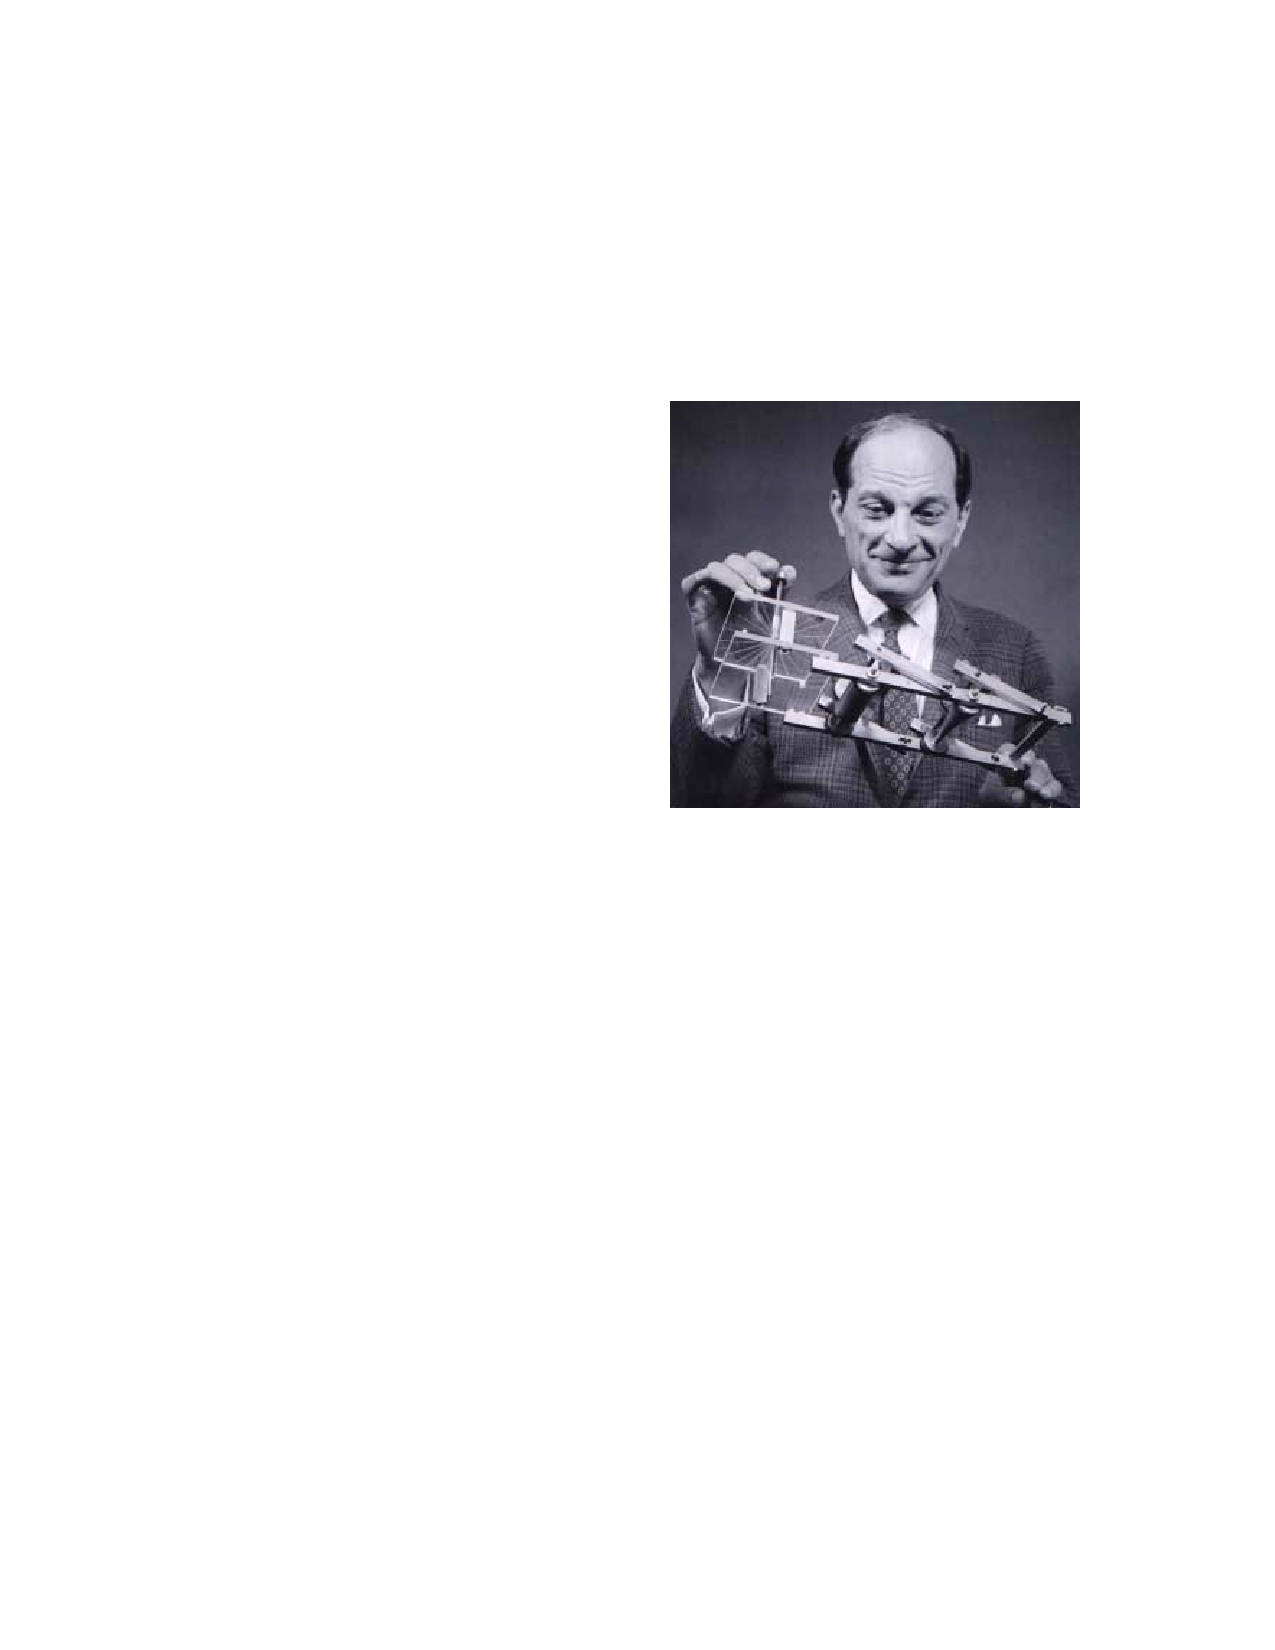
\includegraphics[width=1.5in]{img/ulam-fermiac.pdf}
\end{minipage}
\end{center}

\newcounter{savepage}
\setcounter{savepage}{\arabic{page} + 1}

\mainmatter
\setcounter{page}{\thesavepage}
\part{Introduction}


\chapter{Overview}

\noindent
This document is both a user's guide and a reference manual for
\Stan's probabilistic modeling language.  This introductory chapter
provides a high-level overview of \Stan.  The next chapter provides a
hands-on quick-start guide showing how \Stan works in practice.
Installation instructions are in \refappendix{install}. The remaining
parts of this document include a practically-oriented user's guide for
programming models and a detailed reference manual for \Stan's
modeling language and associated programs and data formats.

\section{Stan Interfaces}

There are three interfaces for Stan that are supported as part of the
Stan project.  Models and their use are the same across the three
interfaces, and this manual is the modeling language manual for all
three interfaces.  All of the interfaces share initialization,
sampling and tuning controls, and roughly share posterior analysis
functionality.   

\subsection{CmdStan}

CmdStan allows Stan to be run from the command line.  In some sense,
CmdStan is the reference implementation of Stan.  This manual
currently doubles as the CmdStan documentation.  In the near term,
the CmdStan documentation will be broken out of this manual and given
its own manual.

\subsection{RStan}

RStan is the R interface to Stan.  The installation and getting
started guide for RStan can be found on GitHub at:

\begin{quote}
\url{https://github.com/stan-dev/rstan/wiki/RStan-Getting-Started}
\end{quote}

\subsection{PyStan}

PyStan is the Python interface to Stan.  The installation and getting
started guide for PyStan can be found on Read the Docs at:

\begin{quote}
\url{https://pystan.readthedocs.org/en/latest/getting_started.html}
\end{quote}



\section{Stan Programs}

A \Stan program defines a statistical model through a conditional
probability function $p(\theta|y;x)$, where $\theta$ is a sequence of
modeled unknown values (e.g., model parameters, latent variables, missing
data, future predictions), $y$ is a sequence of modeled known 
values, and $x$ is a sequence of unmodeled predictors and constants
(e.g., sizes, hyperparameters).

\Stan programs consist of variable type declarations and statements.
Variable types include constrained and unconstrained integer, scalar,
vector, and matrix types, as well as (multidimensional) arrays of
other types.  Variables are declared in blocks corresponding to the
variable's use: data, transformed data, parameter, transformed
parameter, or generated quantity.  Unconstrained local variables may
be declared within statement blocks.

Statements in \Stan are interpreted imperatively, so their order
matters.  Atomic statements involve the assignment of a value to a
variable.  Sequences of statements (and optionally local variable
declarations) may be organized into a block.  \Stan also provides bounded
for-each loops of the sort used in \R and \BUGS.

The transformed data, transformed parameter, and generated quantities
blocks contain statements defining the variables declared in their
blocks.  A special model block consists of statements defining the log
probability for the model.

Within the model block, \BUGS-style sampling notation may be used as
shorthand for incrementing an underlying log probability variable, the
value of which defines the log probability function.  The log
probability variable may also be accessed directly, allowing
user-defined probability functions and Jacobians of transforms.


\section{Compiling and Running \Stan Programs}

A \Stan program is first compiled to a \Cpp program by the \Stan
compiler \stanc, then the \Cpp program compiled to a self-contained
platform-specific executable.  \Stan can generate executables for
various flavors of Windows, Mac OS X, and Linux.%
%
\footnote{A \Stan program may also be compiled to a dynamically
  linkable object file for use in a higher-level scripting language
  such as \R or Python.}
%
Running the \Stan executable for a model first reads in and validates
the known values $y$ and $x$, then generates a sequence of
(non-independent) identically distributed samples $\theta^{(1)},
\theta^{(2)}, \ldots$, each of which has the marginal distribution
$p(\theta|y;x)$.


\section{Sampling}

For continuous parameters, \Stan uses Hamiltonian Monte Carlo (\HMC)
sampling \citep{Duane:1987, Neal:1994, Neal:2011}, a form of Markov chain Monte
Carlo (\MCMC) sampling \citep{Metropolis:1953}.  \Stan 1.0 does not do
discrete sampling.%
%
\footnote{Plans are in place to add full discrete sampling in \Stan
  2.0.  An intermediate step will be to allow forward sampling of
  discrete variables in the generated quantities block for predictive
  modeling and model checking.}
%
\refchapter{mixture-modeling} discusses how finite discrete parameters
can be summed out of models.

\HMC accelerates both convergence to the stationary distribution and
subsequent parameter exploration by using the gradient of the log
probability function.  The unknown quantity vector $\theta$ is
interpreted as the position of a fictional particle.  Each iteration
generates a random momentum and simulates the path of the particle
with potential energy determined the (negative) log probability
function.  Hamilton's decomposition shows that the gradient of this
potential determines change in momentum and the momentum determines
the change in position.  These continuous changes over time are
approximated using the leapfrog algorithm, which breaks the time into
discrete steps which are easily simulated.  A Metropolis reject step
is then applied to correct for any simulation error and ensure
detailed balance of the resulting Markov chain transitions
\citep{Metropolis:1953, Hastings:1970}.

Standard \HMC involves three ``tuning'' parameters to which its
behavior is quite sensitive.  \Stan's samplers allow these parameters
to be set by hand or set automatically without user intervention.

The first two tuning parameters set the temporal step size of the
discretization of the Hamiltonian and the total number of steps taken
per iteration (with their product determining total simulation time).
\Stan can be configured with a user-specified step size or it can
estimate an optimal step size during warmup using dual averaging
\citep{Nesterov:2009, Hoffman-Gelman:2011, Hoffman-Gelman:2013}.  
In either case, additional randomization may be applied to draw the 
step size from an interval of possible step sizes \citep{Neal:2011}.

\Stan can be set to use a specified number of steps, or it can
automatically adapt the number of steps during sampling using the
No-U-Turn (\NUTS) sampler 
\citep{Hoffman-Gelman:2011, Hoffman-Gelman:2013}.  

The third tuning parameter is a mass matrix for the fictional
particle.  \Stan can be configured to estimate a diagonal mass matrix
or a full mass matrix during warmup; Stan will support user-specified
mass matrices in the future.  Estimating a diagonal mass matrix
normalizes the scale of each element $\theta_k$ of the unknown
variable sequence $\theta$, whereas estimating a full mass matrix
accounts for both scaling and rotation,%
%
\footnote{These estimated mass matrices are global, meaning they are
  applied to every point in the parameter space being sampled.
  Riemann-manifold HMC generalizes this to allow the curvature implied
  by the mass matrix to vary by position.}
%
but is more memory and computation intensive per leapfrog step due to
the underlying matrix operations.

\subsection{Convergence Monitoring and Effective Sample Size}

Samples in a Markov chain are only drawn with the marginal
distribution $p(\theta|y;x)$ after the chain has converged to its
equilibrium distribution.  There are several methods to test whether
an \MCMC method has failed to converge; unfortunately, passing the
tests does not guarantee convergence.  The recommended method for
\Stan is to run multiple Markov chains each with different diffuse
initial parameter values, discard the warmup/adaptation samples, then
split the remainder of each chain in half and compute the potential
scale reduction statistic, $\hat{R}$ \citep{GelmanRubin:1992}.

When estimating a mean based on $M$ independent samples, the
estimation error is proportional to $1/\sqrt{M}$.  If the samples are
positively correlated, as they typically are when drawn using \MCMC
methods, the error is proportional to $1/\sqrt{\mbox{\sc ess}}$, where
{\sc ess} is the effective sample size.  Thus it is standard practice
to also monitor (an estimate of) the effective sample size of
parameters of interest in order to estimate the additional estimation
error due to correlated samples.

\subsection{Bayesian Inference and Monte Carlo Methods}

\Stan was developed to support full Bayesian inference.  Bayesian
inference is based in part on Bayes's rule,
\[
p(\theta|y;x) \propto p(y|\theta;x) \, p(\theta;x),
\]
which, in this unnormalized form, states that the posterior
probability $p(\theta|y;x)$ of parameters $\theta$ given data $y$ (and
constants $x$) is proportional (for fixed $y$ and $x$) to the
product of the likelihood function $p(y|\theta;x)$ and prior
$p(\theta;x)$.

For \Stan, Bayesian modeling involves coding the posterior probability
function up to a proportion, which Bayes's rule shows is equivalent to
modeling the product of the likelihood function and prior up to a
proportion.

Full Bayesian inference involves propagating the uncertainty in the
value of parameters $\theta$ modeled by the posterior $p(\theta|y;x)$.
This can be accomplished by basing inference on a sequence of samples
from the posterior using plug-in estimates for quantities of interest
such as posterior means, posterior intervals, predictions based on the
posterior such as event outcomes or the values of as yet unobserved
data.


\section{Optimization}

\Stan also supports optimization-based inference for models.  Given a
posterior $p(\theta|y)$, Stan can find the posterior mode $\theta^*$,
which is defined by
%
\[
\theta^{*} = \mbox{argmax}_{\theta} \ p(\theta|y).
\]
%
Here the notation $\mbox{argmax}_u \ f(v)$ is used to pick out the value
of $v$ at which $f(v)$ is maximized.  

If the prior is uniform, the posterior mode corresponds to the maximum
likelihood estimate (MLE) of the parameters.  If the prior is not
uniform, the posterior mode is sometimes called the maximum a
posterior (MAP) estimate.  If parameters (typically hierarchical) have
been marginalized out, it's sometimes called a maximum marginal
likelihood (MML) estimate. 


\subsection{Inference with Point Estimates}

The estimate $\theta^{*}$ is a so-called ``point estimate,'' meaning
that it summarizes the posterior distribution by a single point,
rather than with a distribution.  Of course, a point estimate does
not, in and of itself, take into account estimation variance.
Posterior predictive inferences $p(\tilde{y} | y)$ can be made using
the posterior mode given data $y$ as $p(\tilde{y}|\theta^*)$, but they
are not Bayesian inferences, even if the model involves a prior,
because they do not take posterior uncertainty into account.  If the
posterior variance is low and the posterior mean is near the posterior
mode, inference with point estimates can be very similar to full
Bayesian inference.

\subsubsection{``Empirical Bayes''}

Fitting point estimates of priors and then using them for subsequent
inference is sometimes called ``empirical Bayes'' (see, e.g.,
\citep{Efron:2012}).%
%
\footnote{The scare quotes on ``empirical Bayes'' are because the
  approach is no more empirical than full Bayes.  Empirical Bayes
  approaches merely ignore some posterior uncertainty to make
  inference more efficient computationally.}
%
Typically these optimizations will be done using maximum marignal
likelihood rather than posterior modes of a full model.  Sometimes
Empirical Bayes point estimates will be obtained using moment matching
(see, e.g., the rat-tumor example in Chapter 5 of
\citep{GelmanCarlinSternRubin:2003}).


\subsection{Experimental Feature}

Stan's optimizers have not been as well tested as its samplers, so
they are still considered an ``experimental'' feature.  We would love
to hear back about successess or failures users have with
optimization.  



\chapter{Getting Started}

\noindent
This chapter is designed to help users get acquainted with the overall
design of the \Stan language and calling \Stan from the command line.
Later chapters are devoted to expanding on the material in this
chapter with full reference documentation.  The content is identical
to that found on the getting-started with the command-line
documentation on the Stan home page, \url{http://mc-stan.org/}.

\section{For BUGS Users}

\refappendix{stan-for-bugs} describes some similarities
and important differences between Stan and BUGS (including WinBUGS,
OpenBUGs, and JAGS).


\section{Installation}

For information about supported versions of Windows, Mac and Linux
platforms along with step-by-step installation instructions, see
\refappendix{install}.

\section{Building Stan}

Building Stan itself works the same way across platforms.
To build Stan, first open a command-line terminal application.  Then change
directories to the directory in which Stan is installed (i.e., the
directory containing the file named \code{makefile}).
%
\begin{quote}
\begin{Verbatim}[fontshape=sl]
> cd <stan-home>
\end{Verbatim}
\end{quote}
%
Then make the library with the following make command
%
\begin{quote}
\begin{Verbatim}[fontshape=sl]
> make bin/libstan.a
\end{Verbatim}
\end{quote}
%
then make the model parser and code generator with the following call,
adjusting the \code{2} in \code{-j2} to the number of CPU cores
available.
%
\begin{quote}
\begin{Verbatim}[fontshape=sl]
> make -j2 bin/stanc
\end{Verbatim}
\end{quote}
%
\emph{Warning:} \ The \code{make} program may take 10+ minutes and
consume 2+ GB of memory to build \code{stanc}.  Compiler warnings,
such as \code{uname:~not found}, may be safely ignored.
 
Finally, make the Stan output summary program with the following
make command.
%
\begin{quote}
\begin{Verbatim}[fontshape=sl]
> make bin/print
\end{Verbatim}
\end{quote}
%

Building \code{libstan.a}, \code{bin/stanc}, and \code{bin/print}
needs to be done only once.

\section{Compiling and Executing a Model}\label{compiling-model.section}

The rest of this quick-start guide explains how to code
and run a very simple Bayesian model.

\subsection{A Simple Bernoulli Model}

The following simple model is available in the source
distribution located at \code{<stan-home>} as
%
\begin{quote}
\nolinkurl{src/models/basic_estimators/bernoulli.stan}
\end{quote}
%
The file contains the following model.
%
\begin{quote}
\begin{Verbatim}
data { 
  int<lower=0> N; 
  int<lower=0,upper=1> y[N];
} 
parameters {
  real<lower=0,upper=1> theta;
} 
model {
  theta ~ beta(1,1);
  for (n in 1:N) 
    y[n] ~ bernoulli(theta);
}
\end{Verbatim}
\end{quote}
%
The model assumes the binary observed data \code{y[1],...,y[N]}
are i.i.d.\ with Bernoulli chance-of-success \code{theta}.  The
prior on \code{theta} is \code{beta(1,1)} (i.e., uniform).

\subsubsection{Implicit Uniform Priors}

If no prior is specified for a parameter, it is implicitly given a
uniform prior on its support.  For parameters such as \code{theta} in
the example, which are constrained to fall between 0 and 1, this
produces a proper uniform distribution on the support of \code{theta}.
Because $\distro{Beta}(1,1)$ is the uniform distribution, the
following sampling statement can be eliminated from the model without
changing the log probability calculation.
%
\begin{quote}
\begin{Verbatim}
  theta ~ beta(1,1);
\end{Verbatim}
\end{quote}

For parameters with unbounded support, the implicit uniform prior is
improper.  Stan allows improper priors to be specified in models, but
posteriors must be proper in order for sampling to succeed.


\subsubsection{Constraints on Parameters}

The variable \code{theta} is defined with lower and upper bounds,
which constrain its value.  Parameters with constrained support should
always specify appropriate constraints in the parameter declaration;
if the constraints are absent, sampling will either slow down or stop
altogether based on whether the initial values satisfy the constraints.

\subsubsection{Vectorizing Sampling Statements}

Iterations of the model will be faster if the loop over sampling
statements is \textit{vectorized} by replacing
%
\begin{quote}
\begin{Verbatim}
  for (n in 1:N) 
    y[n] ~ bernoulli(theta);
\end{Verbatim}
\end{quote}
%
with the equivalent vectorized form,
%
\begin{quote}
\begin{Verbatim}
  y ~ bernoulli(theta);
\end{Verbatim}
\end{quote}
%
Performance gains from vectorization are not because loops are slow in
Stan, but because calls to sampling statements are slow.
Vectorization allows multiple calls to a sampling statement to be
replaced with a single call that can share common calculations for the
log probability function, its gradients, and error checking.  For more
tips on optimizing the performance of Stan models, see
\refchapter{optimization}.


\subsection{Data Set}

A data set of $\mbox{\code{N}}=10$ observations is available in the file
%
\begin{quote}
\nolinkurl{src/models/basic_estimators/bernoulli.data.R}
\end{quote}
%
The content of the file is as follows.
%
\begin{quote}
\begin{Verbatim}
N <- 10
y <- c(0,1,0,0,0,0,0,0,0,1)
\end{Verbatim}
\end{quote}
%
This defines the contents of two variables, \code{N} and \code{y},
using an R-like syntax (see \refchapter{dump} for more information).



\subsection{Generating and Compiling the Model}

A single call to \code{make} will generate the \Cpp code for a
model with a name ending in \code{.stan} and compile it for
execution.  This call will also compile the library \code{libstan.a}
and the parser/code generator \code{stanc} if they have not already
been compiled.

First, change directories to \code{<stan-home>}, the directory where
Stan was unpacked that contains the file named \code{makefile} and
a subdirectory called \code{src/}.
%
\begin{quote}
\begin{Verbatim}[fontshape=sl]
> cd <stan-home>
\end{Verbatim}
\end{quote}
%
Then issue the following command:
%
\begin{quote}
\begin{Verbatim}[fontshape=sl]
> make src/models/basic_estimators/bernoulli 
\end{Verbatim}
\end{quote}
%
The command for Windows is the same, including the forward slashes.

The \code{make} command may be applied to files in locations
that are not subdirectories issued from another directory as follows.
Just replace the relative path \code{src/models/...} with the
actual path.

The C++ generated for the model and its compiled executable
form will be placed in the same directory as the model.


\subsection{Sampling from the Model}

The model can be executed from the directory in which it resides.
%
\begin{quote}
\begin{Verbatim}[fontshape=sl]
> cd src/models/basic_estimators 
\end{Verbatim}
\end{quote}
%
To execute sampling of the model under Linux or Mac, use
%
\begin{quote}
\begin{Verbatim}[fontshape=sl]
> ./bernoulli sample data file=bernoulli.data.R
\end{Verbatim}
\end{quote}
%
The \code{./} prefix before the executable is only required under
Linux and the Mac when executing a model from the directory in which
it resides.

For the Windows DOS terminal, the \code{./} prefix is not needed,
resulting in the following command.
%
\begin{quote}
\begin{Verbatim}[fontshape=sl]
> bernoulli sample data file=bernoulli.data.R
\end{Verbatim}
\end{quote}
%
Whether the command is run in Windows, Linux, or on the Mac, the
output is the same.  First, the parameters are echoed to the standard output,
which shows up on the terminal as follows.
%
\begin{quote}
\begin{Verbatim}[fontsize=\small]
 method = sample (Default)
   sample
     num_samples = 1000 (Default)
     num_warmup = 1000 (Default)
     save_warmup = 0 (Default)
     thin = 1 (Default)
     adapt
       engaged = 1 (Default)
       gamma = 0.050000000000000003 (Default)
       delta = 0.80000000000000004 (Default)
       kappa = 0.75 (Default)
       t0 = 10 (Default)
       init_buffer = 75 (Default)
       term_buffer = 50 (Default)
       window = 25 (Default)
     algorithm = hmc (Default)
       hmc
         engine = nuts (Default)
           nuts
             max_depth = 10 (Default)
         metric = diag_e (Default)
         stepsize = 1 (Default)
         stepsize_jitter = 0 (Default)
 id = 0 (Default)
 data
   file = bernoulli.data.R
 init = 2 (Default)
 random
   seed = 4294967295 (Default)
 output
   file = output.csv (Default)
   diagnostic_file =  (Default)
   refresh = 100 (Default)
...
\end{Verbatim}
\end{quote}
%
The ellipses (\code{...}) indicate that the output continues (as
described below).

After the configuration has been displayed a short timing warning
is given.
%
\begin{quote}
\begin{Verbatim}[fontsize=\small]
...
Gradient evaluation took 4e-06 seconds
1000 transitions using 10 leapfrog steps per transition would take 0.04 seconds.
Adjust your expectations accordingly!
...
\end{Verbatim}
\end{quote}

Next, the sampler counts up the iterations in place, reporting
percentage completed, ending as follows.
%
\begin{quote}
\begin{Verbatim}[fontsize=\small]
...
Iteration:    1 / 2000 [  0%]  (Warmup)
...
Iteration: 1000 / 2000 [ 50%]  (Warmup)
Iteration: 1001 / 2000 [ 50%]  (Sampling)
...
Iteration: 2000 / 2000 [100%]  (Sampling)
...
\end{Verbatim}
\end{quote}

\subsubsection{Sampler Output}

Each execution of the model results in the samples from a single
Markov chain being written to a file in comma-separated value (CSV) format.
The default name of the output file is \nolinkurl{output.csv}.

The first part of the output file just repeats the parameters
as comments (i.e., lines beginning with the pound sign (\Verb|#|)).
%
\begin{quote}
\begin{Verbatim}[fontsize=\small]
# stan_version_major = 2
# stan_version_minor = 1
# stan_version_patch = 0
# model = bernoulli_model
# method = sample (Default)
#   sample
#     num_samples = 1000 (Default)
#     num_warmup = 1000 (Default)
#     save_warmup = 0 (Default)
#     thin = 1 (Default)
#     adapt
#       engaged = 1 (Default)
#       gamma = 0.050000000000000003 (Default)
#       delta = 0.80000000000000004 (Default)
#       kappa = 0.75 (Default)
#       t0 = 10 (Default)
#       init_buffer = 75 (Default)
#       term_buffer = 50 (Default)
#       window = 25 (Default)
#     algorithm = hmc (Default)
#       hmc
#         engine = nuts (Default)
#           nuts
#             max_depth = 10 (Default)
#         metric = diag_e (Default)
#         stepsize = 1 (Default)
#         stepsize_jitter = 0 (Default)
# id = 0 (Default)
# data
#   file = bernoulli.data.R
# init = 2 (Default)
# random
#   seed = 355899897
# output
#   file = output.csv (Default)
#   diagnostic_file =  (Default)
#   refresh = 100 (Default)
...
\end{Verbatim}
\end{quote}
%
This is then followed by a header indicating the
names of the values sampled.
%
\begin{quote}
\begin{Verbatim}[fontsize=\small]
...
lp__,accept_stat__,stepsize__,treedepth__,n_leapfrog__,n_divergent__,theta
...
\end{Verbatim}
\end{quote}
%
The first column gives the log probability.  The next columns, here
columns two through five, provide sampler-dependent information. For
basic Hamiltonian Monte Carlo (HMC) and its adaptive variant No-U-Turn
sampler (NUTS), the sampler-depedent parameters are described in the
following table.
%
\begin{center}
\begin{tabular}{l|l|l}
{\it Sampler} & {\it Parameter} & {\it Description} 
\\ \hline \hline
\HMC & \Verb| accept_stat__ | &  Metropolis acceptance probability
\\
\HMC & \Verb| stepsize__  | & Integrator step size
\\
\HMC & \Verb| int_time__  | & Total integration time
\\
\NUTS & \Verb| accept_stat__  | & Metropolis acceptance probability
\\
& & averaged over samples in the slice 
\\
\NUTS & \Verb| stepsize__ | & Integrator step size
\\
\NUTS & \Verb| treedepth__  | & Tree depth
\\
\NUTS & \Verb| n_leapfrog__  | & Number of leapfrog calculations
\\
\NUTS & \Verb| n_divergent__  | & Number of divergent iterations
\\
\end{tabular}
\end{center}
%
The rest of the columns in the header correspond to model parameters, here
just \code{theta} in the sixth column.  The parameter name header is
output before warmup begins.

The result of any adaptation taking place during warmup is output next
after the parameter names.  
%
\begin{quote}
\begin{Verbatim}[fontsize=\small]
...
# Adaptation terminated
# Step size = 1.81311
# Diagonal elements of inverse mass matrix:
# 0.415719
...
\end{Verbatim}
\end{quote}
%
The default sampler is NUTS with an adapted step size and a diagonal
inverse mass matrix.  For the running example, the step size is
1.81311, and the inverse mass contains the single entry 0.415719
corresponding to the parameter \code{theta}.

Samples from each iteration are printed out next, one per line in
columns corresponding to the headers.
%
\footnote{There are repeated entries due to the Metropolis accept step
in the No-U-Turn sampling algorithm.}
%
%
\begin{quote}
\begin{Verbatim}[fontsize=\small]
...
-6.95293,0.945991,1.09068,2,3,0.335074
-6.92373,0.938744,1.09068,1,1,0.181194
-6.83655,0.934833,1.09068,2,3,0.304882
...
-7.01732,1,1.09068,1,1,0.348244
-8.96652,0.48441,1.09068,1,1,0.549066
-7.22574,1,1.09068,1,1,0.383089
\end{Verbatim}
\end{quote}
%

The output ends with timing details,%
\begin{quote}
\begin{Verbatim}[fontsize=\small]
...
#  Elapsed Time: 0.006811 seconds (Warm-up)
#                0.011645 seconds (Sampling)
#                0.018456 seconds (Total)
\end{Verbatim}
\end{quote}


\subsubsection{Summarizing Sampler Output}

The command-line program \code{bin/print} will display summary
information about the run (for more information, see
\refchapter{print-command}). To run \code{print} on the output file
generated for \code{bernoulli} on Linux or Mac,  use
%
\begin{quote}
\begin{Verbatim}[fontshape=sl]
> <stan-home>/bin/print output.csv
\end{Verbatim}
\end{quote}
%
where \code{<stan-home>} is the path to where Stan was unpacked.  For
Windows use backslashes for the executable,
%
\begin{quote}
\begin{Verbatim}[fontshape=sl]
> <stan-home>\bin\print output.csv
\end{Verbatim}
\end{quote}
%
The output of the command will display information about the run
followed by information for each parameter and generated quantity. For
\code{bernoulli}, we ran 1 chain and saved 1000 iterations. The
information is echoed to the standard output stream.  For the running
example, the path to \code{<stan-home>} can be specified from the
directory in which the Bernoulli model resides using \code{../} (with
backslashes on Windows) as
%
\begin{quote}
\begin{Verbatim}[fontshape=sl]
> ../../../bin/print output.csv 
\end{Verbatim}
\end{quote}
%
For Windows, reverse the slashes.  The output is
%
\begin{Verbatim}[fontshape=sl,fontsize=\footnotesize]
Inference for Stan model: bernoulli_model
1 chains: each with iter=(1000); warmup=(0); thin=(1); 1000 iterations saved.

Warmup took (0.0066) seconds, 0.0066 seconds total
Sampling took (0.011) seconds, 0.011 seconds total

                 Mean     MCSE   StdDev        5%   50%   95%  N_Eff  N_Eff/s  R_hat
lp__             -7.3  3.5e-02  6.9e-01  -8.7e+00  -7.0  -6.7    390    34020   1.00
accept_stat__    0.64  1.2e-02  3.6e-01   5.1e-03  0.74   1.0    882    76898   1.00
stepsize__        1.8  7.8e-15  5.6e-15   1.8e+00   1.8   1.8   0.50       44   1.00
treedepth__     0.076  8.6e-03  2.7e-01   0.0e+00  0.00   1.0    942    82167   1.00
n_leapfrog__     2.7  4.9e-02  1.3e+00    1.0   3.0   3.0    716    65090  1.0e+00
n_divergent__    0.00  0.0e+00  0.0e+00   0.0e+00  0.00  0.00   1000    90909   1.00
theta            0.25  4.2e-03  1.2e-01   9.0e-02  0.23  0.47    827    72146   1.00

Samples were drawn using hmc with nuts.
For each parameter, N_Eff is a crude measure of effective sample size,
and R_hat is the potential scale reduction factor on split chains (at 
convergence, R_hat=1).
\end{Verbatim}
%
In addition to the general information about the runs, \code{print}
displays summary statistics for each parameter and generated
quantity.

In the \code{bernoulli} model, there is a single parameter,
\code{theta}. The mean, standard error of the mean, standard
deviation, the 5\%, 50\%, and 95\% quantiles, number of effective
samples (total and per second), and $\hat{R}$ value are displayed.
These quantities and their uses are described in detail in
\refchapter{mcmc}.

The command \code{bin/print} can be called with more than one csv file
by separating filenames with spaces. It will also take wildcards in
specifying filenames. A typical usage of Stan from the command line
would first create one or more Markov chains by calling the model
executable, typically in parallel, writing the output CSV file for
each into its own directory.  Next, after all of the processes are
finished, the results would be analyzed using \code{print} to assess
convergence and inspect the means and quantiles of the fitted
variables.  Additionally, downstream inferences may be performed using
the samples (e.g., to make decisions or predictions for unseen data).

\subsection{Optimization}

Stan can be used for finding posterior modes as well as sampling from
the posterior.   The model does not need to be recompiled in order to
switch from optimization to sampling, and the data input format is the
same.  Although many command-line arguments may be provided to
configure the optimizer, the following minimal command suffices, using
defaults for everything but where to find the data file.
%
\begin{quote}
\begin{Verbatim}[fontshape=sl]
./bernoulli optimize data file=bernoulli.data.R
\end{Verbatim}
\end{quote}
%
which prints out
%
\begin{quote}
\begin{Verbatim}[fontsize=\footnotesize]
 method = optimize
   optimize
     algorithm = bfgs (Default)
       bfgs
         init_alpha = 0.001 (Default)
         tol_obj = 1e-08 (Default)
         tol_grad = 1e-08 (Default)
         tol_param = 1e-08 (Default)
     iter = 2000 (Default)
     save_iterations = 0 (Default)
 id = 0 (Default)
 data
   file = bernoulli.data.R
 init = 2 (Default)
 random
   seed = 2907588507
 output
   file = output.csv (Default)
   append_sample = 0 (Default)
   diagnostic_file =  (Default)
   append_diagnostic = 0 (Default)
   refresh = 100 (Default)

initial log joint probability = -10.9308
    Iter      log prob        ||dx||      ||grad||    alpha  # evals  Notes 
       7      -5.00402   3.67055e-07   3.06339e-11        1       10   
Optimization terminated normally: 
  Convergence detected: change in objective function was below
  tolerance
\end{Verbatim}
\end{quote}
%
The first part of the output reports on the configuration used, here
indicating the default BFGS optimizer, with default initial stepsize
and tolerances for monitoring convergence.  The second part of the
output indicates how well the algorithm fared, here converging and
terminating normally.  The numbers reported indicate that it took 7
iterations and 10 gradient evaluations, resulting in a final state
state where the change in parameters was roughly 3.7e-7 and the length
of the gradient roughly 3e-11.  The \code{alpha} value is for step
size used.  This is, not surprisingly, far fewer iterations than
required for sampling; even fewer iterations would be used with less
stringent user-specified convergence tolerances.


\subsubsection{Output from Optimization}

The output from optimization is written into the file
\code{output.csv} by default.  The output follows the same pattern as the
output for sampling, first dumping the entire set of parameters used.
%
\begin{quote}
\begin{Verbatim}[fontsize=\small]
# stan_version_major = 2
# stan_version_minor = 1
# stan_version_patch = 0
# model = bernoulli_model
# method = optimize
#   optimize
#     algorithm = bfgs (Default)
#       bfgs
#         init_alpha = 0.001 (Default)
#         tol_obj = 1e-08 (Default)
#         tol_grad = 1e-08 (Default)
#         tol_param = 1e-08 (Default)
#     iter = 2000 (Default)
#     save_iterations = 0 (Default)
# id = 0 (Default)
# data
#   file = bernoulli.data.R
# init = 2 (Default)
# random
#   seed = 2907588507
# output
#   file = output.csv (Default)
#   append_sample = 0 (Default)
#   diagnostic_file =  (Default)
#   append_diagnostic = 0 (Default)
#   refresh = 100 (Default)
lp__,theta
-5.00402,0.2000000000030634
\end{Verbatim}
\end{quote}
%
Note that everything is a comment other than a line for the header,
and a line for the values.  Here, the header indicates the
unnormalized log probability with \code{lp\_\_} and the model
parameter \code{theta}.  The maximum log probability is -5.0 and the
posterior mode for \code{theta} is 0.20.  The mode exactly matches
what we would expect from the data.  
%
\footnote{The Jacobian adjustment included for the sampler's log
  probability function is not applied during optimization, because it can
  change the shape of the posterior and hence the solution.}
%
Because the prior was uniform, the result 0.20 represents the maximum
likelihood estimate (MLE) for the very simple Bernoulli model.  Note
that no uncertainty is reported.  


\subsection{Configuring Command-Line Options}

The command-line options for running a model are detailed in
\refchapter{stan-cmd}. They can also be printed on the command line
using Linux or Mac OS with
%
\begin{quote}
\begin{Verbatim}[fontshape=sl]
> ./bernoulli help-all
\end{Verbatim}
\end{quote}
%
and on Windows with
%
\begin{quote}
\begin{Verbatim}[fontshape=sl]
> bernoulli help-all
\end{Verbatim}
\end{quote}
%
It may help to glance at the command-line skeletons in
\reffigure{nuts-command} through \reffigure{diagnostic-command} to get
a handle on the options then read the detailed descriptions earlier in
\refchapter{stan-cmd}.

\subsection{Testing Stan}

To run the Stan unit tests of basic functionality, run the
following commands from a shell (where \code{<stan-home>} is replaced
top-level directory into which Stan was unpacked; it should contain a
file named \code{makefile}).
%
\begin{quote}
\begin{Verbatim}[fontshape=sl]
> cd <stan-home>
> make -j4 O=0 test-unit
> make -j4 O=0 test-distributions
> make -j4 O=3 test-models
\end{Verbatim}
\end{quote}
%
As before, \code{-j4} indicates that four processes should be run in
parallel; adjust the value \code{4} to correspond to the number of CPU
cores available. Code optimization is specified by the letter `O'
followed by an equal sign followed by the digit `0' for no
optimization and `3' for more optimization; optimization slows down
compilation of the executable but reduces its execution time.
Warnings can be safely ignored if the tests complete without a
\code{FAIL} error.

\emph{Warning}: \ The unit tests can take 30+ minutes and consume 3+
GB of memory with the default compiler, \code{g++}.  The distribution
test and model tests can take even longer.  It is faster to run the
Clang compiler (option \code{CC=clang++}), and to run in multiple
processes in parallel (e.g., option \code{-j4} for four threads).



\part{Modeling Language Reference}

\chapter{Execution of a Stan Program}

\noindent
This chapter provides a sketch of how a compiled Stan model is
executed using sampling.  Optimization shares the same data reading
and initialization steps, but then does optimization rather than sampling.

This sketch is elaborated in the following chapters of this part,
which cover variable declarations, expressions, statements, and blocks
in more detail.


\section{Reading and Transforming Data}

The reading and transforming data steps are the same for sampling,
optimization and diagnostics.

\subsection{Read Data}

The first step of execution is to read data into memory.   Data may be
read in through file (in CmdStan) or through memory (RStan and
PyStan);  see their respective manuals for details.%
%
\footnote{The \Cpp code underlying Stan is flexible enough to allow
  data to be read from memory or file.  Calls from \R, for instance,
  can be configured to read data from file or directly from \R's
  memory.}
%
All of the variables declared in the \code{data} block will be read.
If a variable cannot be read, the program will halt with a message
indicating which data variable is missing.

After each variable is read, if it has a declared constraint, the
constraint is validated.  For example, if a variable \code{N} is
declared as \code{int<lower=0>}, after \code{N} is read, it will be tested
to make sure it is greater than or equal to zero.  If a variable
violates its declared constraint, the program will halt with a warning
message indicating which variable contains an illegal value, the value
that was read, and the constraint that was declared.

\subsection{Define Transformed Data}

After data is read into the model, the transformed data variable
statements are executed in order to define the transformed data
variables.  As the statements execute, declared constraints on
variables are not enforced.

Transformed data variables are initialized with real values set to
\code{NaN} and integer values set to the smallest integer (large
absolute value negative number).

After the statements are executed, all declared constraints on
transformed data variables are validated.  If the validation fails,
execution halts and the variable's name, value and constraints are
displayed.

\section{Initialization}

Initialization is the same for sampling, optimization, and diagnosis

\subsection{User-Supplied Initial Values}

If there are user-supplied initial values for parameters, these are
read using the same input mechanism and same file format as data
reads.  Any constraints declared on the parameters are validated for
the initial values.  If a variable's value violates its declared
constraint, the program halts and a diagnostic message is printed.

After being read, initial values are transformed to unconstrained
values that will be used to initialize the sampler.

\subsubsection{Boundary Values are Problematic}

Because of the way Stan defines its transforms from the constrained to
the unconstrained space, initializing parameters on the boundaries of
their constraints is usually problematic.  For instance, with a
constraint
%
\begin{stancode}
parameters {
  real<lower=0,upper=1> theta;
  // ...
}
\end{stancode}
%
an initial value of 0 for \code{theta} leads to an unconstrained value
of $-\infty$, whereas a value of 1 leads to an unconstrained value of
$+\infty$.  While this will be inverse transformed back correctly
given the behavior of floating point arithmetic, the Jacobian will be
infinite and the log probability function will fail and raise an
exception.

\subsection{Random Initial Values}

If there are no user-supplied initial values, the default
initialization strategy is to initialize the unconstrained parameters
directly with values drawn uniformly from the interval $(-2,2)$.  The
bounds of this initialization can be changed but it is always
symmetric around 0. The value of 0 is special in that it represents
the median of the initialization.  An unconstrained value of 0
corresponds to different parameter values depending on the constraints
declared on the parameters.

An unconstrained real does not involve any transform, so an initial
value of 0 for the unconstrained parameters is also a value of 0 for
the constrained parameters.

For parameters that are bounded below at 0, the initial value of 0 on
the unconstrained scale corresponds to $\exp(0) = 1$ on the
constrained scale.  A value of -2 corresponds to $\exp(-2) = .13$ and
a value of 2 corresponds to $\exp(2) = 7.4$.

For parameters bounded above and below, the initial value of 0 on the
unconstrained scale corresponds to a value at the midpoint of the
constraint interval.  For probability parameters, bounded below by 0
and above by 1, the transform is the inverse logit, so that an initial
unconstrained value of 0 corresponds to a constrained value of 0.5, -2
corresponds to 0.12 and 2 to 0.88.  Bounds other than 0 and 1 are
just scaled and translated.

Simplexes with initial values of 0 on the unconstrained basis
correspond to symmetric values on the constrained values (i.e., each
value is $1/K$ in a $K$-simplex).

Cholesky factors for positive-definite matrices are initialized to 1
on the diagonal and 0 elsewhere;  this is because the diagonal is log
transformed and the below-diagonal values are unconstrained.

The initial values for other parameters can be determined from the
transform that is applied.  The transforms are all described in full
detail in \refchapter{variable-transforms}.

\subsection{Zero Initial Values}

The initial values may all be set to 0 on the unconstrained scale.
This can be helpful for diagnosis, and may also be a good starting
point for sampling.  Once a model is running, multiple chains with
more diffuse starting points can help diagnose problems with
convergence; see \refsection{convergence} for more information on
convergence monitoring.





\section{Sampling}

Sampling is based on simulating the Hamiltonian of a particle with a
starting position equal to the current parameter values and an initial
momentum (kinetic energy) generated randomly.  The potential energy at
work on the particle is taken to be the negative log (unnormalized) total
probability function defined by the model.  In the usual approach to
implementing \HMC, the Hamiltonian dynamics of the particle is
simulated using the leapfrog integrator, which discretizes the smooth
path of the particle into a number of small time steps called leapfrog
steps.

\subsection{Leapfrog Steps}

For each leapfrog step, the negative log probability function and its
gradient need to be evaluated at the position corresponding to the
current parameter values (a more detailed sketch is provided in the
next section).  These are used to update the momentum based on the
gradient and the position based on the momentum.

For simple models, only a few leapfrog steps with large step sizes are
needed.  For models with complex posterior geometries, many small
leapfrog steps may be needed to accurately model the path of the
parameters.

If the user specifies the number of leapfrog steps (i.e., chooses to
use standard \HMC), that number of leapfrog steps are simulated.  If
the user has not specified the number of leapfrog steps, the No-U-Turn
sampler (\NUTS) will determine the number of leapfrog steps adaptively
\citep{Hoffman-Gelman:2011, Hoffman-Gelman:2014}.

\subsection{Log Probability and Gradient Calculation}

During each leapfrog step, the log probability function and its
gradient must be calculated.  This is where most of the time in the
Stan algorithm is spent.  This log probability function, which is
used by the sampling algorithm, is defined over the unconstrained
parameters.

The first step of the calculation requires the inverse transform of
the unconstrained parameter values back to the constrained parameters
in terms of which the model is defined.  There is no error checking
required because the inverse transform is a total function on every point
in whose range satisfies the constraints.

Because the probability statements in the model are defined in terms
of constrained parameters, the log Jacobian of the inverse transform
must be added to the accumulated log probability.

Next, the transformed parameter statements are executed.  After they
complete, any constraints declared for the transformed parameters are
checked.  If the constraints are violated, the model will halt with a
diagnostic error message.

The final step in the log probability function calculation is to
execute the statements defined in the model block.

As the log probability function executes, it accumulates an in-memory
representation of the expression tree used to calculate the log
probability.  This includes all of the transformed parameter
operations and all of the Jacobian adjustments.  This tree is then
used to evaluate the gradients by propagating partial derivatives
backward along the expression graph.  The gradient calculations
account for the majority of the cycles consumed by a Stan program.

\subsection{Metropolis Accept/Reject}

A standard Metropolis accept/reject step is required to retain detailed
balance and ensure samples are marginally distributed according to the
probability function defined by the model.  This Metropolis adjustment
is based on comparing log probabilities, here defined by the
Hamiltonian, which is the sum of the potential (negative log
probability) and kinetic (squared momentum) energies.  In theory, the
Hamiltonian is invariant over the path of the particle and rejection
should never occur.  In practice, the probability of rejection is
determined by the accuracy of the leapfrog approximation to the true
trajectory of the parameters.

If step sizes are small, very few updates will be rejected, but many
steps will be required to move the same distance.  If step sizes are
large, more updates will be rejected, but fewer steps will be required
to move the same distance.  Thus a balance between effort and
rejection rate is required.  If the user has not specified a step
size, Stan will tune the step size during warmup sampling to achieve
a desired rejection rate (thus balancing rejection versus number of
steps).

If the proposal is accepted, the parameters are updated to their new
values.  Otherwise, the sample is the current set of parameter values.


\section{Optimization}

Optimization runs very much like sampling in that it starts by reading
the data and then initializing parameters.  Unlike sampling, it
produces a deterministic output which requires no further analysis
other than to verify that the optimizer itself converged to a
posterior mode.  The output for optimization is also similar to that
for sampling.


\section{Variational Inference}

Variational inference also runs similar to sampling. It begins by reading the
data and initializing the algorithm. The initial variational approximation is a
random draw from the standard normal distribution in the unconstrained
(real-coordinate) space. Again, similar to sampling, it outputs samples from the
approximate posterior once the algorithm has decided that it has converged.
Thus, the tools we use for analyzing the result of Stan's sampling routines can
also be used for variational inference.



\section{Model Diagnostics}

Model diagnostics are like sampling and optimization in that they
depend on a model's data being read and its parameters being
initialized.  The user's guides for the interfaces (RStan, PyStan,
CmdStan) provide more details on the diagnostics available; as of Stan
2.0, that's just gradients on the unconstrained scale and log
probabilities.

\section{Output}

For each final sample (not counting samples during warmup or samples
that are thinned), there is an output stage of writing the samples.

\subsection{Generated Quantities}

Before generating any output, the statements in the generated quantities
block are executed.  This can be used for any forward simulation based
on parameters of the model.  Or it may be used to transform parameters
to an appropriate form for output.

After the generated quantities statements execute, the constraints
declared on generated quantities variables are validated.   If these
constraints are violated, the program will terminate with a diagnostic message.

\subsection{Write}

The final step is to write the actual values.  The values of all
variables declared as parameters, transformed parameters, or generated
quantities are written.  Local variables are not written, nor is the
data or transformed data.  All values are written in their constrained
forms, that is the form that is used in the model definitions.

In the executable form of a Stan models, parameters, transformed
parameters, and generated quantities are written to a file in
comma-separated value (\acronym{csv}) notation with a header defining
the names of the parameters (including indices for multivariate
parameters).%
\footnote{In the \R version of Stan, the values may either be
written to a \acronym{csv} file or directly back to \R's memory.}

% PSEUDOCODE FOR STAN MODEL
% \begin{verbatim}
% read data into memory
% validate data constraints
% execute transformed data statements
% validate transformed data constraints
% read and inverse transform initial parameter values
%     (OR randomly initialize)
% for each sample desired:
%     if warming up and adapting, adapt step size
%     randomly initialize momentum
%     for each leapfrog step:
%         calculate log probability and gradient
%         increment momentum by half step-size times gradient
%         increment parameters by step-size times momentum
%         calculate log probability and gradient
%         increment momentum by half step-size times gradient
%     if not rejected by Metropolis condition:
%         update parameters to new values
%         execute transformed parameters statement
%         validate transformed parameters constraints
%         write parameters, transformed parameters, generated quantities
% \end{verbatim}



\chapter{Data Types and Variable Declarations}\label{data-types.chapter}

\noindent
This chapter covers the data types for expressions in Stan.  Every
variable used in a Stan program must have a declared data type.  Only
values of that type will be assignable to the variable (except for
temporary states of transformed data and transformed parameter
values).  This follows the convention of programming languages like
\Cpp, not the conventions of scripting languages like Python or
statistical languages such as \R or \BUGS.

The motivation for strong, static typing is threefold.
%
\begin{itemize}
\item Strong typing forces the programmer's intent to be declared with
  the variable, making programs easier to comprehend and hence easier
  to debug and maintain.
\item Strong typing allows programming errors relative to the declared
  intent to be caught sooner (at compile time) rather than later (at
  run time).  The Stan compiler (called through an interface such as
  CmdStan, RStan, or PyStan) will flag any type errors and indicate
  the offending expressions quickly when the program is compiled.
\item Constrained types will catch runtime data, initialization, and
  intermediate value errors as soon as they occur rather than allowing
  them to propagate and potentially pollute final results.
\end{itemize}
%
Strong typing disallows assigning the same variable to objects of
different types at different points in the program or in different
invocations of the program.

\section{Overview of Data Types}

\subsection{Basic Data Types}

The primitive Stan data types are \code{real} for continuous scalar
quantities and \code{int} for integer values.  The compound data
types include \code{vector} (of real values), \code{row\_vector} (of
real values), and \code{matrix} (of real values).

\subsection{Constrained Data Types}

Integer or real types may be constrained with lower bounds, upper
bounds, or both.  There are four constrained vector data types,
\code{simplex} for unit simplexes, \code{unit\_vector} for unit-length
vectors, \code{ordered} for ordered vectors of scalars and
\code{positive\_ordered} for vectors of positive ordered scalars.
There are specialized matrix data types \code{corr\_matrix} and
\code{cov\_matrix} for correlation matrices (symmetric, positive
definite, unit diagonal) and covariance matrices (symmetric, positive
definite).  The type \code{cholesky\_factor\_cov} is for Cholesky
factors of covariance matrices (lower triangular, positive diagonal,
product with own transpose is a covariance matrix).  The type
\code{cholesky\_factor\_corr} is for Cholesky factors of correlation
matrices (lower triangular, positive diagonal, unit-length rows).

\subsection{Arrays}

Stan supports arrays of arbitrary order of any of the basic data
types or constrained basic data types.  This includes
three-dimensional arrays of integers, one-dimensional arrays of
positive reals, four-dimensional arrays of simplexes, one-dimensional
arrays of row vectors, and so on.



\section{Primitive Numerical Data Types}\label{numerical-data-types.section}

Unfortunately, the lovely mathematical abstraction of integers and
real numbers is only partially supported by finite-precision computer
arithmetic.

\subsection{Integers}

Stan uses 32-bit (4-byte) integers for all of its integer
representations.  The maximum value that can be represented
as an integer is $2^{31}-1$; the minimum value is $-(2^{31})$.

When integers overflow, their values wrap.  Thus it is up to the Stan
programmer to make sure the integer values in their programs stay in
range.  In particular, every intermediate expression must have an
integer value that is in range.

Integer arithmetic works in the expected way for addition,
subtraction, and multiplication, but rounds the result of division
(see \refsection{int-arithmetic} for more information).

\subsection{Reals}

Stan uses 64-bit (8-byte) floating point representations of real
numbers.  Stan roughly%
%
\footnote{Stan compiles integers to \code{int} and reals to
  \code{double} types in \Cpp.  Precise details of rounding will depend
  on the compiler and hardware architecture on which the code is run.}
%
follows the {\sc ieee} 754 standard for floating-point computation.
The range of a 64-bit number is roughly $\pm 2^{1022}$, which is
slightly larger than $\pm 10^{307}$.  It is a good idea to stay well
away from such extreme values in Stan models as they are prone to
cause overflow.

64-bit floating point representations have roughly 15 decimal digits
of accuracy.  But when they are combined, the result often has less
accuracy.  In some cases, the difference in accuracy between two
operands and their result is large.

There are three special real values used to represent (1) error
conditions, (2) positive infinity, and (3) negative infinity.  The
error value is referred to as ``not a number.''

\subsection{Promoting Integers to Reals}

Stan automatically promotes integer values to real values if
necessary, but does not automatically demote real values to integers.
For very large integers, this will cause a rounding error to fewer
significant digits in the floating point representation than in the
integer representation.

Unlike in \Cpp, real values are never demoted to integers.  Therefore,
real values may only be assigned to real variables.  Integer values
may be assigned to either integer variables or real variables.
Internally, the integer representation is cast to a floating-point
representation.  This operation is not without overhead and should
thus be avoided where possible.


\section{Univariate Data Types and Variable Declarations}

All variables used in a Stan program must have an explicitly declared
data type.  The form of a declaration includes the type and the name
of a variable.  This section covers univariate types, the next section
vector and matrix types, and the following section array types.

\subsection{Unconstrained Integer}

Unconstrained integers are declared using the \code{int} keyword.
For example, the variable \code{N} is declared to be an integer as follows.
%
\begin{stancode}
int N;
\end{stancode}
%

\subsection{Constrained Integer}

Integer data types may be constrained to allow values only in a
specified interval by providing a lower bound, an upper bound, or
both.  For instance, to declare \code{N} to be a positive integer, use
the following.
%
\begin{stancode}
int<lower=1> N;
\end{stancode}
%
This illustrates that the bounds are inclusive for integers.

To declare an integer variable \code{cond} to take only binary values,
that is zero or one, a lower and upper bound must be provided, as in
the following example.
%
\begin{stancode}
int<lower=0,upper=1> cond;
\end{stancode}


\subsection{Unconstrained Real}

Unconstrained real variables are declared using the keyword
\code{real}, The following example declares \code{theta} to be an
unconstrained continuous value.
%
\begin{stancode}
real theta;
\end{stancode}
%

\subsection{Constrained Real}

Real variables may be bounded using the same syntax as integers.  In
theory (that is, with arbitrary-precision arithmetic), the bounds on
real values would be exclusive.  Unfortunately, finite-precision
arithmetic rounding errors will often lead to values on the
boundaries, so they are allowed in Stan.

The variable \code{sigma} may be declared to be non-negative as follows.
%
\begin{stancode}
real<lower=0> sigma;
\end{stancode}
%
The following declares the variable \code{x} to be less than or equal
to $-1$.
%
\begin{stancode}
real<upper=-1> x;
\end{stancode}
%
To ensure \code{rho} takes on values between $-1$ and $1$, use the
following declaration.
%
\begin{stancode}
real<lower=-1,upper=1> rho;
\end{stancode}
%

\subsubsection{Infinite Constraints}

Lower bounds that are negative infinity or upper bounds that are
positive infinity are ignored.  Stan provides constants
\code{positive\_infinity()} and \code{negative\_infinity()} which may
be used for this purpose, or they may be read as data in the dump
format.


\subsection{Expressions as Bounds}

Bounds for integer or real variables may be arbitrary expressions.
The only requirement is that they only include variables that have
been defined before the declaration.  If the bounds themselves are
parameters, the behind-the-scenes variable transform accounts for them
in the log Jacobian.

For example, it is acceptable to have the
following declarations.
%
\begin{stancode}
data {
 real lb;
}
parameters {
   real<lower=lb> phi;
}
\end{stancode}
%
This declares a real-valued parameter \code{phi} to take values
greater than the value of the real-valued data variable \code{lb}.
Constraints may be complex expressions, but must be of type \code{int}
for integer variables and of type \code{real} for real variables
(including constraints on vectors, row vectors, and matrices).
Variables used in constraints can be any variable that has been
defined at the point the constraint is used.  For instance,
\begin{stancode}
data {
   int<lower=1> N;
   real y[N];
}
parameters {
   real<lower=min(y), upper=max(y)> phi;
}
\end{stancode}
%
This declares a positive integer data variable \code{N}, an array
\code{y} of real-valued data of length \code{N}, and then a parameter
ranging between the minimum and maximum value of \code{y}.  As shown
in the example code, the functions \code{min()} and \code{max()} may
be applied to containers such as arrays.


\section{Vector and Matrix Data Types}

\subsection{Values}

Vectors, row vectors, and matrices contain real values.  Arrays, on
the other hand, may contain any kind of value, including integers and
structured values like vectors.

\subsection{Indexing from 1}

Vectors and matrices, as well as arrays, are indexed starting from one
in Stan.  This follows the convention in statistics and linear
algebra as well as their implementations in the statistical software
packages \R, \MATLAB, \BUGS, and \JAGS.  General computer programming
languages, on the other hand, such as \Cpp and Python, index arrays
starting from zero.


\subsection{Vectors}

Vectors in Stan are column vectors; see the next subsection for
information on row vectors.  Vectors are declared with a size (i.e., a
dimensionality).  For example, a 3-dimensional vector is declared with
the keyword \code{vector}, as follows.
%
\begin{stancode}
vector[3] u;
\end{stancode}
%
Vectors may also be declared with constraints, as in the following
declaration of a 3-vector of non-negative values.
%
\begin{stancode}
vector<lower=0>[3] u;
\end{stancode}
%




\subsection{Unit Simplexes}

A unit simplex is a vector with non-negative values whose entries sum
to 1.  For instance, $(0.2,0.3,0.4,0.1)^{\top}$ is a unit 4-simplex.
Unit simplexes are most often used as parameters in categorical
or multinomial distributions, and they are also the sampled variate in
a Dirichlet distribution.  Simplexes are declared with their full
dimensionality.  For instance, \code{theta} is declared to
be a unit $5$-simplex by
%
\begin{stancode}
simplex[5] theta;
\end{stancode}
%

Unit simplexes are implemented as vectors and may be assigned to other
vectors and vice-versa.  Simplex variables, like other constrained
variables, are validated to ensure they contain simplex values; for
simplexes, this is only done up to a statically specified accuracy
threshold $\epsilon$ to account for errors arising from floating-point
imprecision.

\subsection{Unit Vectors}

A unit vector is a vector with a norm of one.  For instance,
$(0.5,0.5,0.5,0.5)^{\top}$ is a unit 4-vector.
Unit vectors are sometimes used in directional statistics.
Unit vectors are declared with their full
dimensionality.  For instance, \code{theta} is declared to
be a unit $5$-vector by
%
\begin{stancode}
unit_vector[5] theta;
\end{stancode}
%
Unit vectors are implemented as vectors and may be assigned to other
vectors and vice-versa.  Unit vector variables, like other constrained
variables, are validated to ensure that they are indeed unit length; for
unit vectors, this is only done up to a statically specified accuracy
threshold $\epsilon$ to account for errors arising from floating-point
imprecision.

\subsection{Ordered Vectors}

An ordered vector type in Stan represents a vector whose entries are
sorted in ascending order.  For instance, $(-1.3,2.7,2.71)^{\top}$ is
an ordered 3-vector.  Ordered vectors are most often employed as cut
points in ordered logistic regression models (see
\refsection{ordered-logistic}).

The variable \code{c} is declared as an ordered 5-vector by
%
\begin{stancode}
ordered[5] c;
\end{stancode}
%
After their declaration, ordered vectors, like unit simplexes, may be
assigned to other vectors and other vectors may be assigned to them.
Constraints will be checked after executing the block in which the
variables were declared.


\subsection{Positive, Ordered Vectors}

There is also a positive, ordered vector type which operates similarly
to ordered vectors, but all entries are constrained to be positive.
For instance, $(2,3.7,4,12.9)$ is a positive, ordered 4-vector.

The variable \code{d} is declared as a positive, ordered 5-vector by
%
\begin{stancode}
positive_ordered[5] d;
\end{stancode}
%
Like ordered vectors, after their declaration positive ordered vectors
assigned to other vectors and other vectors may be assigned to them.
Constraints will be checked after executing the block in which the
variables were declared.

\subsection{Row Vectors}

Row vectors are declared with the keyword \code{row\_vector}.
Like (column) vectors, they are declared with a size.  For example,
a 1093-dimensional row vector \code{u} would be declared as
%
\begin{stancode}
row_vector[1093] u;
\end{stancode}
%
Constraints are declared as for vectors, as in the following example
of a 10-vector with values between -1 and 1.
\begin{stancode}
row_vector<lower=-1,upper=1>[10] u;
\end{stancode}
%

Row vectors may not be assigned to column vectors, nor may column
vectors be assigned to row vectors.  If assignments are required, they
may be accommodated through the transposition operator.

\subsection{Matrices}

Matrices are declared with the keyword \code{matrix} along with a
number of rows and number of columns.  For example,
%
\begin{stancode}
matrix[3,3] A;
matrix[M,N] B;
\end{stancode}
%
declares \code{A} to be a $3 \times 3$ matrix and \code{B} to be a $M
\times N$ matrix.  For the second declaration to be well formed, the
variables \code{M} and \code{N} must be declared as integers in either
the data or transformed data block and before the matrix declaration.

Matrices may also be declared with constraints, as in this ($3 \times $4)
matrix of non-positive values.
%
\begin{stancode}
matrix<upper=0>[3,4] B;
\end{stancode}
%

\subsubsection{Assigning to Rows of a Matrix}

Rows of a matrix can be assigned by indexing the left-hand side of an
assignment statement. For example, this is possible.
%
\begin{stancode}
matrix[M,N] a;
row_vector[N] b;
// ...
a[1] = b;
\end{stancode}
%
This copies the values from row vector \code{b} to \code{a[1]}, which
is the first row of the matrix \code{a}.  If the number of columns in
\code{a} is not the same as the size of \code{b}, a run-time error is
raised;  the number of rows of \code{a} is \code{N}, which is also the
size of \code{b}.

Assignment works by copying values in Stan.  That means any subsequent
assignment to \code{a[1]} does not affect \code{b}, nor does an
assignment to \code{b} affect \code{a}.


\subsection{Correlation Matrices}

Matrix variables may be constrained to represent correlation matrices.
A matrix is a correlation matrix if it is symmetric and positive
definite, has entries between $-1$ and $1$, and has a unit diagonal.
Because correlation matrices are square, only one dimension needs
to be declared.  For example,
%
\begin{stancode}
corr_matrix[3] Sigma;
\end{stancode}
%
declares \code{Sigma} to be a $3 \times 3$ correlation matrix.

Correlation matrices may be assigned to other matrices, including
unconstrained matrices, if their dimensions match, and vice-versa.

\subsection{Cholesky Factors of Correlation Matrices}

Matrix variables may be constrained to represent the Cholesky factors
of a correlation matrix.

A Cholesky factor for a correlation matrix $L$ is a $K \times K$
lower-triangular matrix with positive diagonal entries and rows that
are of length 1 (i.e., $\sum_{n=1}^K L_{m,n}^2 = 1$).  If $L$ is a
Cholesky factor for a correlation matrix, then $L\,L^{\top}$ is a
correlation matrix (i.e., symmetric postive definite with a unit
diagonal).

A declaration such as
follows.
%
\begin{stancode}
cholesky_factor_corr[K] L;
\end{stancode}
%
declares \code{L} to be a Cholesky factor for a \code{K} by \code{K}
correlation matrix.

\subsection{Covariance Matrices}

Matrix variables may be constrained to represent covariance matrices.
A matrix is a covariance matrix if it is symmetric and positive
definite.  Like correlation matrices, covariance matrices only need a
single dimension in their declaration.  For instance,
%
\begin{stancode}
cov_matrix[K] Omega;
\end{stancode}
%
declares \code{Omega} to be a $K \times K$ covariance matrix, where
$K$ is the value of the data variable \code{K}.

\subsection{Cholesky Factors of Covariance Matrices}

Matrix variables may be constrained to represent the Cholesky factors
of a covariance matrix.  This is often more convenient or more
efficient than representing covariance matrices directly.

A Cholesky factor $L$ is an $M \times N$ lower-triangular matrix (if
$m < n$ then $L[m,n] =0$) with a positive diagonal ($L[k,k] = 0$) and
$M \geq N$.  If $L$ is a Cholesky factor, then $\Sigma = L \, L^{\top}$
is a covariance matrix.  Furthermore, every covariance matrix has a
Cholesky factorization.

The typical case of a square Cholesky factor may be declared with a
single dimension,
%
\begin{stancode}
cholesky_factor_cov[4] L;
\end{stancode}
%
In general, two dimensions may be declared, with the above being equal to
\code{cholesky\_factor\_cov[4,4]}.  The
type \code{cholesky\_factor\_cov[M,N]} may be used for the general
$M \times N$.

\subsection{Assigning Constrained Variables}

Constrained variables of all types may be assigned to other variables
of the same unconstrained type and vice-versa.  For instance, a
variable declared to be \code{real<lower=0,upper=1>} could be assigned
to a variable declared as \code{real} and vice-versa.  Similarly, a
variable declared as \code{matrix[3,3]} may be assigned to a variable
declared as \code{cov\_matrix[3]} or
\code{cholesky\_factor\_cov[3]}, and vice-versa.

Checks are carried out at the end of each relevant block of statements
to ensure constraints are enforced.  This includes run-time size
checks.  The Stan compiler isn't able to catch the fact that an
attempt may be made to assign a matrix of one dimensionality to a
matrix of mismatching dimensionality.


\subsection{Expressions as Size Declarations}

Variables may be declared with sizes given by expressions.  Such
expressions are constrained to only contain data or transformed data
variables.  This ensures that all sizes are determined once the data
is read in and transformed data variables defined by their statements.
For example, the following is legal.
%
\begin{stancode}
data {
  int<lower=0> N_observed;    int<lower=0> N_missing;
  // ...
transformed parameters {
  vector[N_observed + N_missing] y;
  // ...
\end{stancode}

\subsection{Accessing Vector and Matrix Elements}

If \code{v} is a column vector or row vector, then \code{v[2]} is the
second element in the vector.  If \code{m} is a matrix, then
\code{m[2,3]} is the value in the second row and third column.

Providing a matrix with a single index returns the specified row.  For
instance, if \code{m} is a matrix, then \code{m[2]} is the second row.
This allows Stan blocks such as
%
\begin{stancode}
matrix[M,N] m;
row_vector[N] v;
real x;
// ...
v = m[2];
x = v[3];   // x == m[2][3] == m[2,3]
\end{stancode}
%
The type of \code{m[2]} is \code{row\_vector} because it is the second
row of \code{m}.  Thus it is possible to write \code{m[2][3]} instead
of \code{m[2,3]} to access the third element in the second row.  When
given a choice, the form \code{m[2,3]} is preferred.%
%
\footnote{As of Stan version 1.0, the form
  \code{m[2,3]} is more efficient because it does not require the
  creation and use of an intermediate expression template for
  \code{m[2]}.  In later versions, explicit calls to \code{m[2][3]}
  may be optimized to be as efficient as \code{m[2,3]} by the Stan
  compiler.\label{array-index-style.footnote}}


\subsection{Size Declaration Restrictions}

An integer expression is used to pick out the sizes of vectors,
matrices, and arrays.  For instance, we can declare a vector of size
\code{M + N} using
%
\begin{stancode}
vector[M + N] y;
\end{stancode}
%
Any integer-denoting expression may be used for the size declaration,
providing all variables involved are either data, transformed data, or
local variables.  That is, expressions used for size declarations may
not include parameters or transformed parameters or generated
quantities.

\section{Array Data Types}\label{array-data-types.section}

Stan supports arrays of arbitrary dimension.  An array's elements may
be any of the basic data types, that is univariate integers,
univariate reals, vectors, row vectors matrices, including all of the
constrained forms.

\subsection{Declaring Array Variables}

Arrays are declared by enclosing the dimensions in square brackets
following the name of the variable.

The variable \code{n} is declared as an array of five integers as follows.
%
\begin{stancode}
int n[5];
\end{stancode}
%
A two-dimensional array of real values with three rows and four columns is
declared with the following.
%
\begin{stancode}
real a[3,4];
\end{stancode}
%
A three-dimensional array \code{z} of positive reals with five rows, four
columns, and two shelves can be declared as follows.
%
\begin{stancode}
real<lower=0> z[5,4,2];
\end{stancode}
%

Arrays may also be declared to contain vectors.  For example,
%
\begin{stancode}
vector[7] mu[3];
\end{stancode}
%
declares \code{mu} to be a 3-dimensional array of 7-vectors.
Arrays may also contain matrices.  The example
%
\begin{stancode}
matrix[7,2] mu[15,12];
\end{stancode}
%
declares a $15 \times 12$-dimensional array of $7 \times 2$ matrices.
Any of the constrained types may also be used in arrays, as in the
declaration
%
\begin{stancode}
cholesky_factor_cov[5,6] mu[2,3,4];
\end{stancode}
%
of a $2 \times 3 \times 4$ array of $5 \times 6$ Cholesky factors of
covariance matrices.

\subsection{Accessing Array Elements and Subarrays}

If \code{x} is a 1-dimensional array of length 5, then \code{x[1]} is
the first element in the array and \code{x[5]} is the last.  For a $3
\times 4$ array \code{y} of two dimensions, \code{y[1,1]} is the first
element and \code{y[3,4]} the last element.  For a three-dimensional
array \code{z}, the first element is \code{z[1,1,1]}, and so on.

Subarrays of arrays may be accessed by providing fewer than the full
number of indexes.  For example, suppose \code{y} is a two-dimensional
array with three rows and four columns.  Then \code{y[3]} is
one-dimensional array of length four.  This means that \code{y[3][1]}
may be used instead of \code{y[3,1]} to access the value of the first
column of the third row of \code{y}.  The form \code{y[3,1]} is the
preferred form (see \refnote{array-index-style} in this chapter).

\subsection{Assigning}

Subarrays may be manipulated and assigned just like any other
variables.  Similar to the behavior of matrices, Stan allows blocks
such as
%
\begin{stancode}
real w[9,10,11];
real x[10,11];
real y[11];
real z;
// ...
x = w[5];
y = x[4];  // y == w[5][4] == w[5,4]
z = y[3];  // z == w[5][4][3] == w[5,4,3]
\end{stancode}
%


\subsection{Arrays of Matrices and Vectors}

Arrays of vectors and matrices are accessed in the same way as arrays
of doubles.  Consider the following vector and scalar declarations.
%
\begin{stancode}
vector[5] a[4,3];
vector[5] b[4];
vector[5] c;
real x;
\end{stancode}
%
With these declarations, the following assignments are legal.
%
\begin{stancode}
b = a[1];      // result is array of vectors
c = a[1,3];    // result is vector
c = b[3];      //   same result as above
x = a[1,3,5];  // result is scalar
x = b[3,5];    //   same result as above
x = c[5];      //   same result as above
\end{stancode}
%
Row vectors and other derived vector types (simplex and ordered)
behave the same way in terms of indexing.

Consider the following matrix, vector and scalar declarations.
%
\begin{stancode}
matrix[6,5] d[3,4];
matrix[6,5] e[4];
matrix[6,5] f;
row_vector[5] g;
real x;
\end{stancode}
%
With these declarations, the following definitions are legal.
%
\begin{stancode}
e = d[1];        // result is array of matrices
f = d[1,3];      // result is matrix
f = e[3];        //   same result as above
g = d[1,3,2];    // result is row vector
g = e[3,2];      //   same result as above
g = f[2];        //   same result as above
x = d[1,3,5,2];  // result is scalar
x = e[3,5,2];    //   same result as above
x = f[5,2];      //   same result as above
x = g[2];        //   same result as above
\end{stancode}
%
As shown, the result \code{f[2]} of supplying a single index to a
matrix is the indexed row, here row 2 of matrix \code{f}.


\subsection{Partial Array Assignment}

Subarrays of arrays may be assigned by indexing on the left-hand side
of an assignment statement.  For example, the following is legal.
%
\begin{stancode}
real x[I,J,K];
real y[J,K];
real z[K];
// ...
x[1] = y;
x[1,1] = z;
\end{stancode}
%
The sizes must match.  Here, \code{x[1]} is a \code{J} by \code{K}
array, as is is \code{y}.

Partial array assignment also works for arrays of matrices, vectors,
and row vectors.


\subsection{Mixing Array, Vector, and Matrix Types}

Arrays, row vectors, column vectors and matrices are not
interchangeable in Stan.  Thus a variable of any one of these
fundamental types is not assignable to any of the others, nor may it
be used as an argument where the other is required (use as arguments
follows the assignment rules).



\subsubsection{Mixing Vectors and Arrays}

For example, vectors cannot be assigned to arrays or vice-versa.
%
\begin{stancode}
real a[4];
vector b[4];
row_vector c[4];
// ...
a = b; // illegal assignment of vector to array
b = a; // illegal assignment of array to vector
a = c; // illegal assignment of row vector to array
c = a; // illegal assignment of array to row vector
\end{stancode}

\subsubsection{Mixing Row and Column Vectors}

It is not even legal to assign row vectors to column vectors or vice
versa.
\begin{stancode}
vector b[4];
row_vector c[4];
// ...
b = c; // illegal assignment of row vector to column vector
c = b; // illegal assignment of column vector to row vector
\end{stancode}
%

\subsubsection{Mixing Matrices and Arrays}

The same holds for matrices, where 2-dimensional arrays may not be
assigned to matrices or vice-versa.

\begin{stancode}
real a[3,4];
matrix[3,4] b;
// ...
a = b;  // illegal assignment of matrix to array
b = a;  // illegal assignment of array to matrix
\end{stancode}
%

\subsubsection{Mixing Matrices and Vectors}

A $1 \times N$ matrix cannot be assigned a row vector or
vice versa.
%
\begin{stancode}
matrix[1,4] a;
row_vector[4] b;
// ...
a = b;  // illegal assignment of row vector to matrix
b = a;  // illegal assignment of matrix to row vector
\end{stancode}
%
Similarly, an $M \times 1$ matrix may not be assigned to a column vector.
%
\begin{stancode}
matrix[4,1] a;
vector[4] b;
// ...
a = b;  // illegal assignment of column vector to matrix
b = a;  // illegal assignment of matrix to column vector
\end{stancode}

\subsection{Size Declaration Restrictions}

An integer expression is used to pick out the sizes of arrays.  The
same restrictions as for vector and matrix sizes apply, namely that
the size is declared with an integer-denoting expression that does not
contain any parameters, transformed parameters, or generated quantities.




\section{Variable Types vs.\ Constraints and Sizes}

The type information associated with a variable only contains the
underlying type and dimensionality of the variable.

\subsection{Type Information Excludes Sizes}

The size associated with a given variable is not part of its data
type.  For example, declaring a variable using
\begin{stancode}
real a[3];
\end{stancode}
%
declares the variable \code{a} to be an array.  The fact that it was
declared to have size 3 is part of its declaration, but not part of
its underlying type.

\subsubsection{When are Sizes Checked?}

Sizes are determined dynamically (at run time) and thus cannot be
type-checked statically when the program is compiled.  As a result,
any conformance error on size will raise a run-time error.  For
example, trying to assign an array of size 5 to an array of size 6
will cause a run-time error.  Similarly, multiplying an $N
\times M$ by a $J \times K$ matrix will raise a run-time error if $M
\neq J$.

\subsection{Type Information Excludes Constraints}

Like sizes, constraints are not treated as part of a variable's type
in Stan when it comes to the compile-time check of operations it may
participate in.  Anywhere Stan accepts a matrix as an argument, it
will syntactically accept a correlation matrix or covariance matrix or
Cholesky factor.  Thus a covariance matrix may be assigned to a matrix
and vice-versa.

Similarly, a bounded real may be assigned to an unconstrained real and
vice-versa.

\subsubsection{When are Function Argument Constraints Checked?}

For arguments to functions, constraints are sometimes, but not always
checked when the function is called.  Exclusions include \Cpp standard
library functions.  All probability functions and cumulative
distribution functions check that their arguments are appropriate at
run time as the function is called.

\subsubsection{When are Declared Variable Constraints Checked?}

For data variables, constraints are checked after the variable is read
from a data file or other source.  For transformed data variables, the
check is done after the statements in the transformed data block have
executed.  Thus it is legal for intermediate values of variables to
not satisfy declared constraints.

For parameters, constraints are enforced by the transform applied and
do not need to be checked.  For transformed parameters, the check is
done after the statements in the transformed parameter block have
executed.

For all blocks defining variables (transformed data, transformed
parameters, generated quantities), real values are initialized to
\code{NaN} and integer values are initialized to the smallest legal
integer (i.e., a large absolute value negative number).

For generated quantities, constraints are enforced after the
statements in the generated quantities block have executed.


\subsection{Type Naming Notation}

In order to refer to data types, it is convenient to have a way to
refer to them.  The type naming notation outlined in this section is
not part of the Stan programming language, but rather a convention
adopted in this document to enable a concise description of a type.

Because size information is not part of a data type, data
types will be written without size information.  For instance,
\code{real[]} is the type of one-dimensional array of reals and
\code{matrix} is the type of matrices.  The three-dimensional integer
array type is written as \code{int[\, , \, ,]}, indicating the number slots
available for indexing.  Similarly, \code{vector[,]} is the type of a
two-dimensional array of vectors.


\chapter{Expressions}

\noindent
An expression is the basic syntactic unit in a Stan program that
denotes a value.  Every expression in a well-formed Stan program has
a type that is determined statically (at compile time).  If an
expressions type cannot be determined statically, the Stan compiler
will report the location of the problem.

This chapter covers the syntax, typing, and usage of the various forms
of expressions in Stan.

\section{Numeric Literals}

The simplest form of expression is a literal that denotes a primitive
numerical value.

\subsection{Integer Literals}

Integer literals represent integers of type \code{int}.  Integer
literals are written in base 10 without any separators.  Integer
literals may contain a single negative sign.  (The expression
\code{{-}-1} is interpreted as the negation of the literal \code{-1}.)

The following list contains well-formed integer literals.
%
\begin{quote}
\code{0}, \ \code{1}, \ \code{-1}, \ \code{256},
\ \code{-127098}, \ \code{24567898765}
\end{quote}
%
Integer literals must have values that fall within the bounds for
integer values (see \refsection{numerical-data-types}).

Integer literals may not contain decimal points (\code{.}).  Thus the
expressions \code{1.} and \code{1.0} are of type \code{real} and may
not be used where a value of type \code{int} is required.

\subsection{Real Literals}

A number written with a period or with scientific notation is assigned
to a the continuous numeric type \code{real}.  Real literals are
written in base 10 with a period (\code{.}) as a separator.  Examples
of well-formed real literals include the following.
%
\begin{quote}
\code{0.0}, \ \code{1.0}, \ \code{3.14}, \ \code{-217.9387}, \
\code{2.7e3}, \ \code{-2E-5}
\end{quote}
%
The notation \code{e} or \code{E} followed by a positive or negative
integer denotes a power of 10 to multiply.  For instance, \code{2.7e3}
denotes $2.7 \times 10^3$ and \code{-2E-5} denotes $-2 \times
10^{-5}$.


\section{Variables}\label{variables.section}

A variable by itself is a well-formed expression of the same type as
the variable.  Variables in Stan consist of \ASCII strings containing
only the basic lower-case and upper-case Roman letters, digits, and
the underscore (\code{\_}) character.  Variables must start with a
letter (\code{a--z} and \code{A--Z}) and may not end with two underscores
(\code{\_\_}).

Examples of legal variable identifiers are as follows.
%
\begin{quote}
\code{a},
\ \code{a3},
\ \code{a\_3},
\ \code{Sigma},
\ \code{my\_cpp\_style\_variable},
\ \code{myCamelCaseVariable}
\end{quote}
%
Unlike in \R and \BUGS, variable identifiers in Stan may not contain
a period character.

\subsection{Reserved Names}

Stan reserves many strings for internal use and these may not be used
as the name of a variable.  An attempt to name a variable after an
internal string results in the \code{stanc} translator halting with an
error message indicating which reserved name was used and its location
in the model code.

\subsubsection{Model Name}

The name of the model cannot be used as a variable within the model.
This is usually not a problem because the default in \code{bin/stanc}
is to append \code{\_model} to the name of the file containing the
model specification.  For example, if the model is in file
\code{foo.stan}, it would not be legal to have a variable named
\code{foo\_model} when using the default model name through
\code{bin/stanc}.  With user-specified model names, variables cannot
match the model.

\subsubsection{User-Defined Function Names}

User-defined function names cannot be used as a variable within the
model.

\subsubsection{Reserved Words from Stan Language}

The following list contains reserved words for Stan's programming
language.  Not all of these features are implemented in Stan yet, but
the tokens are reserved for future use.
%
\begin{quote}
\code{for},
\code{in},
\code{while},
\code{repeat},
\code{until},
\code{if},
\code{then},
\code{else},
\code{true},
\code{false}
\end{quote}
%
Variables should not be named after types, either, and thus may not be
any of the following.
%
\begin{quote}
\code{int},
\code{real},
\code{vector},
\code{simplex},
\code{unit\_vector},
\code{ordered},
\code{positive\_ordered},
\code{row\_vector},
\code{matrix},
\code{cholesky\_factor\_corr},
\code{cholesky\_factor\_cov},
\code{corr\_matrix},
\code{cov\_matrix}.
\end{quote}
%
Variable names will {\it not}\ conflict with the following block identifiers,
%
\begin{quote}
\code{functions},
\code{model},
\code{data},
\code{parameters},
\code{quantities},
\code{transformed},
\code{generated},
\end{quote}
%

\subsubsection{Reserved Names from Stan Implementation}

Some variable names are reserved because they are used within
Stan's \Cpp implementation.  These are
%
\begin{quote}
\code{var},
\code{fvar},
\code{STAN\_MAJOR},
\code{STAN\_MINOR},
\code{STAN\_PATCH},
\code{STAN\_MATH\_MAJOR},
\code{STAN\_MATH\_MINOR},
\code{STAN\_MATH\_PATCH}
\end{quote}
%

\subsubsection{Reserved Function and Distribution Names}

Variable names will conflict with the names of predefined functions
other than constants.  Thus a variable may not be named \code{logit}
or \code{add}, but it may be named \code{pi} or \code{e}.

Variable names will also conflict with the names of distributions
suffixed with \code{\_lpdf}, \code{\_lpmf}, \code{\_lcdf}, and
\code{\_lccdf}, \code{\_cdf}, and \code{\_ccdf}, such as
\code{normal\_lcdf\_log}; this also holds for the deprecated forms
\code{\_log}, \code{\_cdf\_log}, and \code{\_ccdf\_log},

Using any of these variable names causes the \code{stanc} translator
to halt and report the name and location of the variable causing the
conflict.


\subsubsection{Reserved Names from C++}

Finally, variable names, including the names of models, should not
conflict with any of the C++ keywords.
%
\begin{quote}
\code{alignas},
\code{alignof},
\code{and},
\code{and\_eq},
\code{asm},
\code{auto},
\code{bitand},
\code{bitor},
\code{bool},
\code{break},
\code{case},
\code{catch},
\code{char},
\code{char16\_t},
\code{char32\_t},
\code{class},
\code{compl},
\code{const},
\code{constexpr},
\code{const\_cast},
\code{continue},
\code{decltype},
\code{default},
\code{delete},
\code{do},
\code{double},
\code{dynamic\_cast},
\code{else},
\code{enum},
\code{explicit},
\code{export},
\code{extern},
\code{false},
\code{float},
\code{for},
\code{friend},
\code{goto},
\code{if},
\code{inline},
\code{int},
\code{long},
\code{mutable},
\code{namespace},
\code{new},
\code{noexcept},
\code{not},
\code{not\_eq},
\code{nullptr},
\code{operator},
\code{or},
\code{or\_eq},
\code{private},
\code{protected},
\code{public},
\code{register},
\code{reinterpret\_cast},
\code{return},
\code{short},
\code{signed},
\code{sizeof},
\code{static},
\code{static\_assert},
\code{static\_cast},
\code{struct},
\code{switch},
\code{template},
\code{this},
\code{thread\_local},
\code{throw},
\code{true},
\code{try},
\code{typedef},
\code{typeid},
\code{typename},
\code{union},
\code{unsigned},
\code{using},
\code{virtual},
\code{void},
\code{volatile},
\code{wchar\_t},
\code{while},
\code{xor},
\code{xor\_eq}
\end{quote}

\subsection{Legal Characters}

The legal variable characters have the same \ASCII code points in the
range 0--127 as in Unicode.
%
\begin{center}
\begin{tabular}{cc}
Characters  & \ASCII (Unicode) Code Points
\\ \hline
\code{a -- z} & \code{{}~97 -- 122}
\\
\code{A -- Z} & \code{{}~65 -- {}~90}
\\
\code{0 -- 9} & \code{{}~48 -- {}~57}\
\\
\code{\_} & \code{95}
\end{tabular}
\end{center}
%
Although not the most expressive character set, \ASCII is the most
portable and least prone to corruption through improper character
encodings or decodings.

\subsubsection{Comments Allow ASCII-Compatible Encoding}

Within comments, Stan can work with any ASCII-compatible character
encoding, such as ASCII itself, UTF-8, or Latin1.  It is up to user
shells and editors to display them properly.


\section{Parentheses for Grouping}

Any expression wrapped in parentheses is also an expression. Like in
\Cpp, but unlike in \R, only the round parentheses, \code{(} and
\code{)}, are allowed.  The square brackets \code{[} and \code{]} are
reserved for array indexing and the curly braces \code{\{} and
\code{\}} for grouping statements.

With parentheses it is possible to explicitly group subexpressions
with operators.  Without parentheses, the expression \code{1 + 2 * 3}
has a subexpression \code{2 * 3} and evaluates to 7.  With
parentheses, this grouping may be made explicit with the expression
\code{1 + (2 * 3)}.  More importantly, the expression \code{(1 + 2) *
  3} has \code{1 + 2} as a subexpression and evaluates to 9.


\section{Arithmetic and Matrix Expressions}\label{arithmetic-expressions.section}

For integer and real-valued expressions, Stan supports the basic
binary arithmetic operations of addition (\code{+}), subtraction
(\code{-}), multiplication (\code{*}) and division (\code{/}) in the
usual ways.

For integer expressions, Stan supports the modulus (\code{\%}) binary
arithmetic operation.  Stan also supports the unary operation of
negation for integer and real-valued expressions.  For example,
assuming \code{n} and \code{m} are integer variables and \code{x} and
\code{y} real variables, the following expressions are legal.
%
\begin{quote}
\code{3.0 + 0.14},
\ \ \code{-15},
\ \ \code{2 * 3 + 1},
\ \ \code{(x - y) / 2.0},
\\
\ \ \code{(n * (n + 1)) / 2},
\ \ \code{x / n},
\ \ \code{m \% n}
\end{quote}
%
The negation, addition, subtraction, and multiplication operations are
extended to matrices, vectors, and row vectors.  The transpose
operation, written using an apostrophe (\code{'}) is also supported
for vectors, row vectors, and matrices.  Return types for matrix
operations are the smallest types that can be statically guaranteed to
contain the result.  The full set of allowable input types and
corresponding return types is detailed in
\refchapter{matrix-operations}.

For example, if \code{y} and \code{mu} are variables of type
\code{vector} and \code{Sigma} is a variable of type \code{matrix},
then
%
\begin{quote}
\code{(y - mu)' * Sigma * (y - mu)}
\end{quote}
%
is a well-formed expression of type \code{real}.  The type of the
complete expression is inferred working outward from the
subexpressions.  The subexpression(s) \code{y - mu} are of type
\code{vector} because the variables \code{y} and \code{mu} are of type
\code{vector}.  The transpose of this expression, the subexpression
\code{(y - mu)'} is of type \code{row\_vector}.  Multiplication is
left associative and transpose has higher precedence than
multiplication, so the above expression is equivalent to the following
well-formed, fully specified form.
%
\begin{quote}
\code{(((y - mu)') * Sigma) * (y - mu)}
\end{quote}
%
The type of subexpression \code{(y - mu)' * Sigma} is inferred to be
\code{row\_vector}, being the result of multiplying a row vector by a
matrix.  The whole expression's type is thus the type of a row vector
multiplied by a (column) vector, which produces a \code{real} value.

Stan provides elementwise matrix division and multiplication
operations, \code{a~.*~b} and \code{a~./b}.  These provide a shorthand
to replace loops, but are not intrinsicially more efficient than a
version programmed with an elementwise calculations and assignments in
a loop.  For example, given declarations,
%
\begin{stancode}
vector[N] a;
vector[N] b;
vector[N] c;
\end{stancode}
%
the assignment,
%
\begin{stancode}
c = a .* b;
\end{stancode}
%
produces the same result with roughly the same efficiency as the loop
%
\begin{stancode}
for (n in 1:N)
  c[n] = a[n] * b[n];
\end{stancode}

Stan supports exponentiation (\code{\textasciicircum}) of integer and
real-valued expressions.  The return type of exponentiation is always
a real-value.  For example, assuming \code{n} and \code{m} are integer
variables and \code{x} and \code{y} real variables, the following
expressions are legal.
%
\begin{quote}
\code{3 \textasciicircum\ 2},
\ \ \code{3.0 \textasciicircum\ -2},
\ \ \code{3.0 \textasciicircum\ 0.14},
\\
\ \ \code{x \textasciicircum\ n},
\ \ \code{n \textasciicircum\ x},
\ \ \code{n \textasciicircum\ m},
\ \ \code{x \textasciicircum\ y}
\end{quote}
%
Exponentiation is right associative, so the expression
%
\begin{quote}
\code{2 \textasciicircum\ 3 \textasciicircum\ 4}
\end{quote}
%
is equivalent to the following well-formed, fully specified form.
%
\begin{quote}
\code{2 \textasciicircum\ (3 \textasciicircum\ 4)}
\end{quote}
%



\subsection{Operator Precedence and Associativity}

The precedence and associativity of operators, as well as built-in
syntax such as array indexing and function application is given in
tabular form in \reffigure{operator-precedence}.
%
\begin{figure}
\begin{center}
\begin{tabular}{c|ccl|l}
{\it Op.} & {\it Prec.} & {\it Assoc.} & {\it
  Placement} & {\it Description}
\\ \hline \hline
\code{?~:} & 10 & right & ternary infix & conditional
\\ \hline
\code{||} & 9 & left & binary infix & logical or
\\ \hline
\Verb|&&| & 8 & left & binary infix & logical and
\\ \hline
\Verb|==| & 7 & left & binary infix & equality
\\
\Verb|!=| & 7 & left & binary infix & inequality
\\ \hline
\Verb|<| & 6 & left & binary infix & less than
\\
\Verb|<=| & 6 & left & binary infix & less than or equal
\\
\Verb|>| & 6 & left & binary infix & greater than
\\
\Verb|>=| & 6 & left & binary infix & greater than or equal
\\ \hline
\code{+} & 5 & left & binary infix & addition
\\
\code{-} & 5 & left & binary infix & subtraction
\\ \hline
\code{*} & 4 & left & binary infix & multiplication
\\
\code{/} & 4 & left & binary infix & (right) division
\\
\code{\%} & 4 & left & binary infix & modulus
\\ \hline
\Verb|\| & 3 & left & binary infix & left division
\\ \hline
\code{.*} & 2 & left & binary infix & elementwise multiplication
\\
\code{./} & 2 & left & binary infix & elementwise division
\\ \hline
\code{!} & 1 & n/a & unary prefix & logical negation
\\
\code{-} & 1 & n/a & unary prefix & negation
\\
\code{+} & 1 & n/a & unary prefix & promotion (no-op in Stan)
\\ \hline
\code{\textasciicircum} & 0.5 & right & binary infix & exponentiation
\\ \hline
\code{'} & 0 & n/a & unary postfix & transposition
\\ \hline \hline
\code{()} & 0 & n/a & prefix, wrap & function application
\\
\code{[]} & 0 & left & prefix, wrap & array, matrix indexing
\end{tabular}
\end{center}
\caption{\small\it Stan's unary, binary, and ternary operators, with their
  precedences, associativities, place in an expression, and a
  description.  The last two lines list the precedence of function
  application and array, matrix, and vector indexing. The operators are
  listed in order of precedence, from least tightly binding to most
  tightly binding.  The full set of legal arguments and corresponding
  result types are provided in the function documentation in
  \refpart{built-in-functions} prefaced with \code{operator} (i.e.,
  \code{operator*(int,int):int} indicates the application of the
  multiplication operator to two integers, which returns an integer).
  Parentheses may be used to group expressions explicitly rather than
  relying on precedence and
  associativity.}\label{operator-precedence.figure}
\end{figure}
%
Other expression-forming operations, such as function application and
subscripting bind more tightly than any of the arithmetic operations.

The precedence and associativity determine how expressions are
interpreted.  Because addition is left associative, the expression
\mbox{\code{a+b+c}} is interpreted as \mbox{\code{(a+b)+c}}.  Similarly,
\mbox{\code{a/b*c}} is interpreted as \mbox{\code{(a/b)*c}}.

Because multiplication has higher precedence than addition, the
expression \mbox{\code{a*b+c}} is interpreted as \mbox{\code{(a*b)+c}} and the
expression \mbox{\code{a+b*c}} is interpreted as \mbox{\code{a+(b*c)}}.  Similarly,
\mbox{\code{2*x+3*-y}} is interpreted as \mbox{\code{(2*x)+(3*(-y))}}.

Transposition and exponentiation bind more tightly
than any other arithmetic or logical operation.
For vectors, row vectors, and matrices,
\mbox{\code{-u'}} is interpreted as \mbox{\code{-(u')}}, \mbox{\code{u*v'}} as
\mbox{\code{u*(v')}}, and \mbox{\code{u'*v}} as \mbox{\code{(u')*v}}.
For integer and reals,
\mbox{\code{-n \textasciicircum\ 3}}
is interpreted as \mbox{\code{-(n \textasciicircum\ 3)}}.


\section{Conditional Operator}\label{conditional-operator.section}

\subsection{Conditional Operator Syntax}

The ternary conditional operator is unique in that it takes three
arguments and uses a mixed syntax.  If \code{a} is an expression of
type \code{int} and \code{b} and \code{c} are expressions that can be
converted to one another (e.g., compared with \code{==}), then 
%
\begin{stancode}
a ? b : c
\end{stancode}
%
is an expression of the promoted type of \code{b} and \code{c}.  The
only promotion allowed in Stan is from integer to real; if one
argument is of type \code{int} and the other of type \code{real}, the
conditional expression as a whole is of type \code{real}.  In all
other cases, the arguments have to be of the same underlying Stan type
(i.e., constraints don't count, only the shape) and the conditional
expression is of that type.

\subsubsection{Conditional Operator Precedence}

The conditional operator is the most loosely binding operator, so its
arguments rarely require parentheses for disambiguation.  For example,
%
\begin{stancode}
a > 0 || b < 0 ? c + d : e - f
\end{stancode}
%
is equivalent to the explicitly grouped version
%
\begin{stancode}
(a > 0 || b < 0) ? (c + d) : (e - f)
\end{stancode}
%
The latter is easier to read even if the parentheses are not strictly
necessary.

\subsubsection{Conditional Operator Associativity}

The conditional operator is right associative, so that
%
\begin{stancode}
a ? b : c ? d : e
\end{stancode}
%
parses as if explicitly grouped as
%
\begin{stancode}
a ? b : (c ? d : e)
\end{stancode}
%
Again, the explicitly grouped version is easier to read.


\subsection{Conditional Operator Semantics}

Stan's conditional operator works very much like its C++ analogue.
The first argument must be an expression denoting an integer.
Typically this is a variable or a relation operator, as in the
variable \code{a} in the example above.  Then there are two resulting
arguments, the first being the result returned if the condition
evaluates to true (i.e., non-zero) and the second if the condition
evaluates to false (i.e., zero).  In the example above, the value
\code{b} is returned if the condition evaluates to a non-zero value
and \code{c} is returned if the condition evaluates to zero.

\subsubsection{Lazy Evaluation of Results}

The key property of the conditional operator that makes it so useful
in high-performance computing is that it only evaluates the returned
subexpression, not the alternative expression.  In other words, it is
not like a typical function that evaluates its argument expressions
eagerly in order to pass their values to the function.  Specifically,
the conditional operator provides a substantial speedup over the
built-in \code{if\_else} function, which, like other functions, evaluates
all three of its arguments when it is called.  As usual, the saving is
mostly in the derivatives that do not get computed rather than the
basic function evaluation itself.

\subsubsection{Promotion to Parameter}

If one return expression is a data value (an expression involving only
constants and variables defined in the data or transformed data
block), and the other is not, then the ternary operator will promote
the data value to a parameter value.  This can cause needless work
calculating derivatives in some cases and be less efficient than a full
\code{if}-\code{then} conditional statement.  For example,
%
\begin{stancode}
data {
  real x[10];
  ...
parameters {
  real z[10];
  ...
model {
  y ~ normal(cond ? x : z, sigma);
  ...
\end{stancode}
%
would be more efficiently (if not more transparently) coded as
%
\begin{stancode}
if (cond)
  y ~ normal(x, sigma);
else
  y ~ normal(z, sigma);
\end{stancode}
%
The conditional statement, like the conditional operator, only
evaluates one of the result statements.  In this case, the variable
\code{x} will not be promoted to a parameter and thus not cause any
needless work to be carried out when propagating the chain rule during
derivative calculations.


\section{Indexing}\label{language-indexing.section}

Stan arrays, matrices, vectors, and row vectors are all accessed
using the same array-like notation.  For instance, if \code{x} is a
variable of type \code{real[]} (a one-dimensional array of reals)
then \code{x[1]} is the value of the first element of the
array.

Subscripting has higher precedence than any of the arithmetic
operations.  For example, \code{alpha*x[1]} is equivalent to
\code{alpha*(x[1])}.

Multiple subscripts may be provided within a single pair of square
brackets.  If \code{x} is of type \code{real[~,~]}, a two-dimensional
array, then \code{x[2,501]} is of type \code{real}.

\subsection{Accessing Subarrays}

The subscripting operator also returns subarrays of arrays.  For
example, if \code{x} is of type \code{real[~,~,~]}, then \code{x[2]}
is of type \code{real[~,~]}, and \code{x[2,3]} is of type
\code{real[]}.  As a result, the expressions \code{x[2,3]} and
\code{x[2][3]} have the same meaning.

\subsection{Accessing Matrix Rows}

If \code{Sigma} is a variable of type \code{matrix}, then
\code{Sigma[1]} denotes the first row of \code{Sigma} and has the
type \code{row\_vector}.

\subsection{Mixing Array and Vector/Matrix Indexes}

Stan supports mixed indexing of arrays and their vector, row vector
or matrix values.  For example, if \code{m} is of type
\code{matrix[,]}, a two-dimensional array of matrices, then
\code{m[1]} refers to the first row of the array, which is a
one-dimensional array of matrices.  More than one index may be used,
so that \code{m[1,2]} is of type \code{matrix} and denotes the matrix
in the first row and second column of the array.  Continuing to add
indices, \code{m[1,2,3]} is of type \code{row\_vector} and denotes
the third row of the matrix denoted by \code{m[1,2]}.  Finally,
\code{m[1,2,3,4]} is of type \code{real} and denotes the value in the
third row and fourth column of the matrix that is found at the first
row and second column of the array \code{m}.

\section{Multiple Indexing}\label{language-multi-indexing.section}

In addition to single integer indexes, as described in
\refsection{language-indexing}, Stan supports multiple indexing.
Multiple indexes can be integer arrays of indexes, lower
bounds, upper bounds, lower and upper bounds, or simply shorthand for
all of the indexes.  A complete table of index types is given in
\reffigure{index-types}.
%
\begin{figure}[t]
\begin{center}
\begin{tabular}{c|c|c}
{\it index type} & {\it example}  & {\it value} \\ \hline \hline
integer & \code{a[11]} 
& value of \code{a} at index 11
\\ \hline
integer array & \code{a[ii]}
& \code{a[ii[1]]}, \ \ldots, \ \code{a[ii[K]]}
\\[4pt]
lower bound & \code{a[3:]} 
& \code{a[3]}, \ \ldots, \ \code{a[N]}
\\
upper bound & \code{a[:5]}
& \code{a[1]}, \ \ldots, \code{a[5]}
\\
range & \code{a[2:7]}
& \code{a[2]}, \ \ldots, \  \code{a[7]}
\\[4pt]
all & \code{a[:]}
& \code{a[1]}, \ldots, \ \code{a[N]}
\\
all & \code{a[]}
& \code{a[1]}, \ldots, \ \code{a[N]}
\end{tabular}
\end{center}
\vspace*{-8pt}
\caption{\small\it Types of indexes and examples with one-dimensional
  containers of size \code{N} and an integer array \code{ii} of type 
\code{int[]} size \code{K}.}\label{index-types.figure}
\end{figure}

\subsection{Multiple Index Semantics}

The fundamental semantic rule for dealing with multiple indexes is the
following.  If \code{idxs} is a multiple index, then it produces an
indexable position in the result.  To evaluate that index position in
the result, the index is first passed to the multiple index, and the
resulting index used.
%
\begin{stancode}
a[idxs, ...][i, ...] = a[idxs[i], ...][...]
\end{stancode}
%
On the other hand, if \code{idx} is a single index, it reduces the
dimensionality of the output, so that
%
\begin{stancode}
a[idx, ...] = a[idx][...]
\end{stancode}

The only issue is what happens with matrices and vectors.  Vectors
work just like arrays.  Matrices with multiple row indexes and
multiple column indexes produce matrices.  Matrices with multiple row
indexes and a single column index become (column) vectors.  Matrices
with a single row index and multiple column indexes become row
vectors.  The types are summarized in \reffigure{matrix-indexing}.
%
\begin{figure}[t]
\begin{center}
\begin{tabular}{c|c|c|c}
{\it example} & {\it row index} & {\it column index} & {\it result type}
\\ \hline \hline
\code{a[i]} &
single & n/a & row vector
\\
\code{a[is]} &
multiple & n/a & matrix
\\ \hline
\code{a[is, js]} & single & single & real
\\
\code{a[i, js]} & single & multiple & row vector
\\
\code{a[is, j]} & multiple & single & vector
\\
\code{a[is, js]} & multiple & multiple & matrix
\end{tabular}
\end{center}
\caption{\small\it Special rules for reducing matrices based on
  whether the argumnt is a single or multiple index.  Examples are for
a matrix \code{a}, with integer single indexes \code{i} and \code{j}
and integer array multiple indexes \code{is} and \code{js}.  The same
typing rules apply for all multiple indexes.}%
\label{matrix-indexing.figure} 
\end{figure}

Evaluation of matrices with multiple indexes is defined to respect the
following distributivity conditions.
%
\begin{stancode}
m[idxs1, idxs2][i, j] = m[idxs1[i], idxs2[j]]
m[idxs, idx][j] = m[idxs[j], idx]
m[idx, idxs][j] = m[idx, idxs[j]]
\end{stancode}
%

Evaluation of arrays of matrices and arrays of vectors or row vectors
is defined recursively, beginning with the array dimensions.


\section{Function Application}\label{function-application.section}

Stan provides a range of built in mathematical and statistical
functions, which are documented in \refpart{built-in-functions}.

Expressions in Stan may consist of the name of function followed by a
sequence of zero or more argument expressions.  For instance,
\code{log(2.0)} is the expression of type \code{real} denoting the
result of applying the natural logarithm to the value of the real
literal \code{2.0}.

Syntactically, function application has higher precedence than any of
the other operators, so that \code{y + log(x)} is interpreted as
\code{y + (log(x))}.

\subsection{Type Signatures and Result Type Inference}

Each function has a type signature which determines the allowable type
of its arguments and its return type.  For instance, the function
signature for the logarithm function can be expressed as
%
\begin{quote}
\code{real log(real);}
\end{quote}
%
and the signature for the \code{lmultiply} function is
%
\begin{quote}
\code{real lmultiply(real,real);}
\end{quote}
%
A function is uniquely determined by its name and its sequence of
argument types.  For instance, the following two functions are
different functions.
%
\begin{quote}
\code{real mean(real[]);}
\\
\code{real mean(vector);}
\end{quote}
%
The first applies to a one-dimensional array of real values and the
second to a vector.

The identity conditions for functions explicitly forbids having two
functions with the same name and argument types but different return
types.  This restriction also makes it possible to infer the type of a
function expression compositionally by only examining the type of its
subexpressions.

\subsection{Constants}

Constants in Stan are nothing more than nullary (no-argument)
functions.  For instance, the mathematical constants $\pi$ and $e$ are
represented as nullary functions named \code{pi()} and \code{e()}.
See \refsection{built-in-constants} for a list of built-in constants.

\subsection{Type Promotion and Function Resolution}

Because of integer to real type promotion, rules must be established
for which function is called given a sequence of argument types.  The
scheme employed by Stan is the same as that used by \Cpp, which
resolves a function call to the function requiring the minimum number
of type promotions.

For example, consider a situation in which the following two function
signatures have been registered for \code{foo}.
%
\begin{quote}
\code{real foo(real,real);}
\\
\code{int foo(int,int);}
\end{quote}
%
The use of \code{foo} in the expression \code{foo(1.0,1.0)} resolves
to \code{foo(real,real)}, and thus the expression \code{foo(1.0,1.0)}
itself is assigned a type of \code{real}.

Because integers may be promoted to real values, the expression
\code{foo(1,1)} could potentially match either \code{foo(real,real)}
or \code{foo(int,int)}.  The former requires two type promotions and
the latter requires none, so \code{foo(1,1)} is resolved to function
\code{foo(int,int)} and is thus assigned the type \code{int}.

The expression \code{foo(1,1.0)} has argument types \code{(int,real)}
and thus does not explicitly match either function signature.  By
promoting the integer expression \code{1} to type \code{real}, it is
able to match \code{foo(real,real)}, and hence the type of the
function expression \code{foo(1,1.0)} is \code{real}.

In some cases (though not for any built-in Stan functions), a
situation may arise in which the function referred to by an
expression remains ambiguous.  For example, consider a situation in
which there are exactly two functions named \code{bar} with the
following signatures.
%
\begin{quote}
\code{real bar(real,int);}
\\
\code{real bar(int,real);}
\end{quote}
%
With these signatures, the expression \code{bar(1.0,1)} and
\code{bar(1,1.0)} resolve to the first and second of the above
functions, respectively.  The expression \code{bar(1.0,1.0)} is
illegal because real values may not be demoted to integers.  The
expression \code{bar(1,1)} is illegal for a different reason.  If the
first argument is promoted to a real value, it matches the first
signature, whereas if the second argument is promoted to a real value,
it matches the second signature.  The problem is that these both
require one promotion, so the function name \code{bar} is ambiguous.
If there is not a unique function requiring fewer promotions than all
others, as with \code{bar(1,1)} given the two declarations above,
the Stan compiler will flag the expression as illegal.

\subsection{Random-Number Generating Functions}

For most of the distributions supported by Stan, there is a
corresponding random-number generating function.  These random number
generators are named by the distribution with the suffix \code{\_rng}.
For example, a univariate normal random number can be generated by
\code{normal\_rng(0,1)};  only the parameters of the distribution,
here a location (0) and scale (1) are specified because the variate is
generated.

\subsubsection{Random-Number Generators Restricted to Generated Quantities Block}

The use of random-number generating functions is restricted to the
generated quantities block; attempts to use them elsewhere will result
in a parsing error with a diagnostic message.

This allows the random number generating functions to be used for
simulation in general, and for Bayesian posterior predictive checking
in particular.

\subsubsection{Posterior Predictive Checking}

Posterior predictive checks typically use the parameters of the model
to generate simulated data (at the individual and optionally at the
group level for hierarchical models), which can then be compared
informally using plots and formally by means of test statistics, to
the actual data in order to assess the suitability of the model; see
\citep[Chapter~6]{GelmanEtAl:2013} for more information on
posterior predictive checks.

\section{Type Inference}

Stan is strongly statically typed, meaning that the implementation
type of an expression can be resolved at compile time.

\subsection{Implementation Types}

The primitive implementation types for Stan are
%
\code{int},
\code{real},
\code{vector},
\code{row\_vector}, and
\code{matrix}.
%
Every basic declared type corresponds to a primitive type;  see
\reffigure{primitive-type} for the mapping from types to their
primitive types.
%
\begin{figure}
\begin{center}
\begin{tabular}{c|c}
{\it Type} & {\it Primitive Type} \\ \hline \hline
\code{int} & \code{int} \\[6pt]
\code{real} & \code{real} \\[6pt]
\code{matrix} & \code{matrix} \\
\code{cov\_matrix} & \code{matrix} \\
\code{corr\_matrix} & \code{matrix} \\
\code{cholesky\_factor\_cov} & \code{matrix} \\
\code{cholesky\_factor\_corr} & \code{matrix} \\[6pt]
\code{vector} & \code{vector} \\
\code{simplex} & \code{vector} \\
\code{unit\_vector} & \code{vector} \\
\code{ordered} & \code{vector} \\
\code{positive\_ordered} & \code{vector} \\[6pt]
\code{row\_vector} & \code{row\_vector}
\end{tabular}
\end{center}
\caption{\it The table shows the variable declaration types of Stan
  and their corresponding primitive implementation type.  Stan
  functions, operators, and probability functions have argument and
  result types declared in terms of primitive types plus array
  dimensionality.}\label{primitive-type.figure}
\end{figure}
%
A full implementation type consists of a primitive implementation type
and an integer array dimensionality greater than or equal to zero.
These will be written to emphasize their array-like nature.  For
example, \code{int[]} has an array dimensionality of 1, \code{int} an
array dimensionality of 0, and \code{int[,,]} an array dimensionality
of 3. The implementation type \code{matrix[,,]} has a total of five
dimensions and takes up to five indices, three from the array and two
from the matrix.

Recall that the array dimensions come before the matrix or vector
dimensions in an expression such as the following declaration of a
three-dimensional array of matrices.
%
\begin{stancode}
matrix[M, N] a[I, J, K];
\end{stancode}
%
The matrix \code{a} is indexed as \code{a[i,j,k,m,n]} with the array
indices first, followed by the matrix indices, with \code{a[i,j,k]}
being a matrix and \code{a[i,j,k,m]} being a row vector.

\subsection{Type Inference Rules}

Stan's type inference rules define the implementation type of an
expression based on a background set of variable declarations.  The
rules work bottom up from primitive literal and variable expressions
to complex expressions.

\subsubsection{Literals}

An integer literal expression such as \code{42} is of type \code{int}.
Real literals such as \code{42.0} are of type \code{real}.

\subsubsection{Variables}

The type of a variable declared locally or in a previous block is
determined by its declaration.  The type of a loop variable is
\code{int}.

There is always a unique declaration for each variable in each scope
because Stan prohibits the redeclaration of an already-declared
variables.%
%
\footnote{Languages such as \Cpp and R allow the declaration of a
  variable of a given name in a narrower scope to hide (take
  precedence over for evaluation) a variable defined in a containing
  scope.}

\subsubsection{Indexing}

If \code{x} is an expression of total dimensionality greater than or
equal to $N$, then the type of expression \code{e[i1,...,iN]} is the
same as that of \code{e[i1]...[iN]}, so it suffices to define the type
of a singly-indexed function.  Suppose \code{e} is an expression and
\code{i} is an expression of primitive type \code{int}.  Then
%
\begin{itemize}
\item if \code{e} is an expression of array dimensionality $K > 0$,
  then \code{e[i]} has array dimensionality $K-1$ and the same
  primitive implementation type as \code{e},
%
\item if \code{e} has implementation type \code{vector} or
  \code{row\_vector} of array dimensionality 0, then \code{e[i]} has
  implementation type \code{real}, and
%
\item if \code{e} has implementation type \code{matrix}, then
  \code{e[i]} has type \code{row\_vector}.
\end{itemize}

\subsubsection{Function Application}

If \code{f} is the name of a function and \code{e1,...,eN} are
expressions for $N \geq 0$, then \code{f(e1,...,eN)} is an expression
whose type is determined by the return type in the function signature
for \code{f} given \code{e1} through \code{eN}.  Recall that a
function signature is a declaration of the argument types and the
result type.

In looking up functions, binary operators like \code{real~*~real} are
defined as \code{operator*(real,real)} in the documentation and index.

In matching a function definition, arguments of type \code{int} may be
promoted to type \code{real} if necessary (see the subsection on type
promotion in \refsection{function-application} for an exact
specification of Stan's integer-to-real type-promotion rule).

In general, matrix operations return the lowest inferrable type.  For
example, \code{row\_vector~*~vector} returns a value of type
\code{real}, which is declared in the function documentation and index
as \code{real~operator*(row\_vector,vector)}.



\section{Chain Rule and Derivatives}

Derivatives of the log probability function defined by a model are
used in several ways by Stan.  The Hamiltonian Monte Carlo samplers,
including NUTS, use gradients to guide updates.  The BFGS optimizers
also use gradients to guide search for posterior modes.

\subsection{Errors Due to Chain Rule}

Unlike evaluations in pure mathematics, evaluation of derivatives in
Stan is done by applying the chain rule on an expression-by-expression
basis, evaluating using floating-point arithmetic.  As a result,
models such as the following are problematic for inference involving
derivatives.
%
\begin{stancode}
parameters {
  real x;
}
model {
  x ~ normal(sqrt(x - x), 1);
}
\end{stancode}
%
Algebraically, the sampling statement in the model could be reduced to
%
\begin{stancode}
  x ~ normal(0, 1);
\end{stancode}
%
and it would seem the model should produce unit normal samples for
\code{x}.  But rather than cancelling, the expression \code{sqrt(x -
  x)} causes a problem for derivatives.  The cause is the mechanistic
evaluation of the chain rule,
%
\begin{eqnarray*}
\frac{d}{dx} \sqrt{x - x}
& = &
\frac{1}{2 \sqrt{x - x}} \times \frac{d}{dx} (x - x)
\\[4pt]
& = &
\frac{1}{0} \times (1 - 1)
\\[4pt]
& = &
\infty \times 0
\\[4pt]
& = & \mbox{NaN}.
\end{eqnarray*}
%
Rather than the $x - x$ cancelling out, it introduces a 0 into the
numerator and denominator of the chain-rule evaluation.

The only way to avoid this kind problem is to be careful to do the
necessary algebraic reductions as part of the model and not introduce
expressions like \code{sqrt(x - x)} for which the chain rule produces
not-a-number values.

\subsection{Diagnosing Problems with Derivatives}

The best way to diagnose whether something is going wrong with the
derivatives is to use the test-gradient option to the sampler or
optimizer inputs; this option is available in both Stan and RStan
(though it may be slow, because it relies on finite differences to
make a comparison to the built-in automatic differentiation).

For example, compiling the above model to an executable
\code{sqrt-x-minus-x}, the test can be run as
%
\begin{Verbatim}
> ./sqrt-x-minus-x diagnose test=gradient
\end{Verbatim}
\begin{Verbatim}[fontsize=\small]
...
TEST GRADIENT MODE

 Log probability=-0.393734

 param idx           value           model     finite diff           error
         0       -0.887393             nan               0             nan
\end{Verbatim}
%
Even though finite differences calculates the right gradient of 0,
automatic differentiation follows the chain rule and produces a
not-a-number output.



\chapter{Statements}

\noindent
The blocks of a Stan program (see \refchapter{blocks}) are made up of
variable declarations and statements.  Unlike programs in \BUGS, the
declarations and statements making up a Stan program are executed in
the order in which they are written.  Variables must be defined to
have some value (as well as declared to have some type) before they
are used --- if they do not, the behavior is undefined.

Like \BUGS, Stan has two kinds of atomic statements, assignment
statements and sampling statements.  Also like \BUGS, statements may
be grouped into sequences and into for-each loops.  In addition, Stan
allows local variables to be declared in blocks and also allows an
empty statement consisting only of a semicolon.

\section{Assignment Statement}\label{assignment-statement.section}

An assignment statement consists of a variable (possibly multivariate
with indexing information) and an expression.  Executing an
assignment statement evaluates the expression on the right-hand side
and assigns it to the (indexed) variable on the left-hand side.  An
example of a simple assignment is as follows.%
%
\footnote{In versions of Stan before 2.10.0, the operator \code{<-} was
  used for assignment rather than using the equal sign \code{=}.  The
  old operator \code{<-} is now deprecated and will print a warning.
  In the future, it will be removed.}
%
\begin{quote}
\code{n = 0;}
\end{quote}
%
Executing this statement assigns the value of the expression \code{0},
which is the integer zero, to the variable \code{n}.  For an assignment
to be well formed, the type of the expression on the right-hand side
should be compatible with the type of the (indexed) variable on the
left-hand side.  For the above example, because \code{0} is an
expression of type \code{int}, the variable \code{n} must be declared
as being of type \code{int} or of type \code{real}.  If the variable
is of type \code{real}, the integer zero is promoted to a
floating-point zero and assigned to the variable.  After the
assignment statement executes, the variable \code{n} will have the
value zero (either as an integer or a floating-point value, depending on
its type).

Syntactically, every assignment statement must be followed by a
semicolon.  Otherwise, whitespace between the tokens does not matter
(the tokens here being the left-hand-side (indexed) variable, the
assignment operator, the right-hand-side expression and the
semicolon).

Because the right-hand side is evaluated first, it is possible to
increment a variable in Stan just as in \Cpp and other programming
languages by writing
%
\begin{quote}
\code{n = n + 1;}
\end{quote}
%
Such self assignments are not allowed in \BUGS, because they induce a
cycle into the directed graphical model.

The left-hand side of an assignment may contain indices for array,
matrix, or vector data structures.  For instance, if \code{Sigma} is
of type \code{matrix}, then
%
\begin{quote}
\code{Sigma[1,1] = 1.0;}
\end{quote}
%
sets the value in the first column of the first row of \code{Sigma} to one.

Assignments can involve complex objects of any type.  If \code{Sigma}
and \code{Omega} are matrices and \code{sigma} is a vector, then the
following assignment statement, in which the expression and variable
are both of type \code{matrix}, is well formed.
%
\begin{stancode}
Sigma
  = diag_matrix(sigma)
     * Omega
     * diag_matrix(sigma);
\end{stancode}
%
This example also illustrates the preferred form of splitting a
complex assignment statement and its expression across lines.

Assignments to subcomponents of larger multi-variate data structures
are supported by Stan.  For example, \code{a} is an array of type
\code{real[~,~]} and \code{b} is an array of type \code{real[]}, then
the following two statements are both well-formed.
%
\begin{stancode}
a[3] = b;
b = a[4];
\end{stancode}
%
Similarly, if \code{x} is a variable declared to have type
\code{row\_vector} and \code{Y} is a variable declared as type
\code{matrix}, then the following sequence of statements to swap the
first two rows of \code{Y} is well formed.
%
\begin{stancode}
x = Y[1];
Y[1] = Y[2];
Y[2] = x;
\end{stancode}
%

\subsection{Lvalue Summary}

The expressions that are legal left-hand sides of assignment
statements are known as ``lvalues.''  In Stan, there are only two
kinds of legal lvalues,
%
\begin{itemize}
\item a variable, or
\item a variable with one or more indices.
\end{itemize}
%
To be used as an lvalue, an indexed variable must have at least as
many dimensions as the number of indices provided.  An array of real
or integer types has as many dimensions as it is declared for.  A
matrix has two dimensions and a vector or row vector one dimension;
this also holds for the constrained types, covariance and correlation
matrices and their Cholesky factors and ordered, positive ordered, and
simplex vectors.  An array of matrices has two more dimensions than
the array and an array of vectors or row vectors has one more
dimension than the array.  Note that the number of indices can be less
than the number of dimensions of the variable, meaning that the right
hand side must itself be multidimensional to match the remaining
dimensions.

\subsection{Multiple Indexes}

Multiple indexes, as described in
\refsection{language-multi-indexing}, are also permitted on the
left-hand side of assignments.  Indexing on the left side works
exactly as it does for expressions, with multiple indexes preserving
index positions and single indexes reducing them.    The type on the
left side must still match the type on the right side.

\subsubsection{Aliasing}

All assignment is carried out as if the right-hand side is copied
before the assignment.  This resolves any potential aliasing issues
arising from he right-hand side changing in the middle of an
assignment statement's execution.



\section{Log Probability Increment Statement}\label{increment-log-prob.section}

The basis of Stan's execution is the evaluation of a log probability
function for a given set of parameters; this function returns the log
density of the posterior up to an additive constant.  Data and
transformed data are fixed before the log density is evaluated.  The
total log probability is initialized to zero.  Next, any log Jacobian
adjustments accrued by the variable constraints are added to the log
density (the Jacobian adjustment may be skipped for optimization).
Sampling and log probability increment statements may add to the log
density in the model block.  A log probability increment statement
directly increments the log density with the value of an expression
as follows.%
%
\footnote{The current notation replaces two previous versions.
  Originally, a variable \code{lp\_\_} was directly exposed and
  manipulated;  this is no longer allowed.  The original statement
  syntax for \code{target += u} was \code{increment\_log\_prob(u)},
  but this form has been deprecated and will be removed in Stan 3.}
%
\begin{stancode}
target += -0.5 * y * y;
\end{stancode}
%
The keyword \code{target} here is actually not a variable, and may not
be accessed as such (though see below on how to access the value of
target through a special function).

In this example, the unnormalized log probability of a unit normal
variable $y$ is added to the total log probability.  In the general
case, the argument can be any expression.%
%
\footnote{Writing this model with the expression \code{-0.5 * y * y}
  is more efficient than with the equivalent expression \code{y * y /
    -2} because multiplication is more efficient than division; in
  both cases, the negation is rolled into the numeric literal
  (\code{-0.5} and \code{-2}).  Writing \code{square(y)} instead of
  \code{y * y} would be even more efficient because the derivatives
  can be precomputed, reducing the memory and number of operations
  required for automatic differentiation.}

An entire Stan model can be implemented this way.  For instance, the
following model will draw a single variable according to a unit normal
probability.
%
\begin{stancode}
parameters {
  real y;
}
model {
  target += -0.5 * y * y;
}
\end{stancode}
%
This model defines a log probability function
%
\[
\log p(y) = - \, \frac{y^2}{2} - \log Z
\]
%
where $Z$ is a normalizing constant that does not depend on $y$.  The
constant $Z$ is conventionally written this way because on the linear
scale,
\[
p(y) = \frac{1}{Z} \exp\left(-\frac{y^2}{2}\right).
\]
which is typically written without reference to $Z$ as
\[
p(y) \propto \exp\left(-\frac{y^2}{2}\right).
\]

Stan only requires models to be defined up to a constant that does not
depend on the parameters.  This is convenient because often the
normalizing constant $Z$ is either time-consuming to compute or
intractable to evaluate.

\subsubsection{Vectorization}

The \code{target += ...} statement accepts an argument in place of
\code{...} for any expression type, including integers, reals,
vectors, row vectors, matrices, and arrays of any dimensionality,
including arrays of vectors and matrices.   For container arguments,
their sum will be added to the total log density.

\subsection{Accessing the Log Density}

To increment the log density returned by the model by some value
\code{u}, use the following statement.%
%
\footnote{Originally, Stan provided direct access to the log density
  through a variable \code{lp\_\_} and then later through the
  \code{increment\_log\_prob()} statement, but the first has been
  removed and the latter deprecated.}
%
\begin{stancode}
target += u;
\end{stancode}
%
In general, \code{u} can be any expression;  if it is a container, the
log density will be incremented by the sum of the elements in the
container.

To access accumulated log density up to the current execution point,
the function \code{get\_lp()} may be used.%
%
\footnote{The value of \code{lp\_\_} will only hold the Jacobian until
  the end of the execution because it is not used in either
  \code{increment\_log\_prob(u)} or \code{target += u}.}


\section{Sampling Statements}\label{sampling-statements.section}

Like \BUGS and \JAGS, Stan supports probability statements in
sampling notation, such as
%
\begin{stancode}
y ~ normal(mu,sigma);
\end{stancode}
%
The name ``sampling statement'' is meant to be suggestive, not
interpreted literally.  Conceptually, the variable \code{y}, which may
be an unknown parameter or known, modeled data, is being declared
to have the distribution indicated by the right-hand side of the
sampling statement.

Executing such a statement does not perform any sampling.  In Stan, a
sampling statement is merely a notational convenience.  The above
sampling statement could be expressed as a direct increment on the
total log probability as
%
\begin{stancode}
target += normal_lpdf(y,mu,sigma);
\end{stancode}
%
See the subsection of \refsection{sampling-statements} discussing log
probability increments for a full explanation.

In general, a sampling statement of the form
%
\begin{stancode}
y ~ dist(theta1, ..., thetaN);
\end{stancode}
%
involving subexpressions \code{y1} and \code{theta1} through
\code{thetaN} (including the case where \code{N} is zero) will be well
formed if and only if the corresponding assignment statement is
well-formed.  For densities allowing real \code{y} values, the log
probability density function is used,
%
\begin{stancode}
target += dist_lpdf(y | theta1, ..., thetaN);
\end{stancode}
%
For those restricted to integer \code{y} values, the log probability
mass function is used,
%
\begin{stancode}
target += dist_lpmf(y | theta1, ..., thetaN);
\end{stancode}
%

This will be well formed if and only if \code{dist\_lpdf(y, theta1,
  ..., thetaN)} or \code{dist\_lpmf(y, theta1, ..., thetaN)} is a
well-formed expression of type \code{real}.

\subsection{Log Probability Increment vs.\ Sampling Statement}

Although both lead to the same sampling behavior in Stan, there is one
critical difference between using the sampling statement, as in
%
\begin{stancode}
y ~ normal(mu, sigma);
\end{stancode}
%
and explicitly incrementing the log probability function, as in
%
\begin{stancode}
target += normal_lpdf(y | mu,sigma);
\end{stancode}
%
The sampling statement drops all the terms in the log probability
function that are constant, whereas the explicit call to
\code{normal\_lpdf} adds all of the terms in the definition of the log
normal probability function, including all of the constant normalizing
terms.  Therefore, the explicit increment form can be used to recreate
the exact log probability values for the model.  Otherwise, the
sampling statement form will be faster if any of the input expressions,
\code{y}, \code{mu}, or \code{sigma}, involve only constants, data
variables, and transformed data variables.


\subsection{User-Transformed Variables}

The left-hand side of a sampling statement may be a complex
expression.  For instance, it is legal syntactically to write
%
\begin{stancode}
data {
  real<lower=0> y;
}
// ...
model {
  log(y) ~ normal(mu, sigma);
}
\end{stancode}
%
Unfortunately, this is not enough to properly model \code{y} as having
a lognormal distribution.  The log Jacobian of the transform must be
added to the log probability accumulator to account for the
differential change in scale (see \refsection{change-of-variables} for
full definitions).  For the case above, the following adjustment will
account for the log transform.%
%
\footnote{Because $\log | \frac{d}{dy} \log y | = \log | 1/y | = - \log
  |y|$;  see \refsection{change-of-variables}.}
%
\begin{stancode}
target += - log(fabs(y));
\end{stancode}
%

\subsection{Truncated Distributions}

A density function $p(x)$ may be truncated to an interval $(a,b)$ to
define a new density $p_{(a,b)}\!(x)$ by setting
%
\[
p_{\!(a,b)\!}(x) = \frac{p(x)}
                  {\int_a^b p(x') \, dx'}.
\]
Given a probability function $p_X(x)$ for a random variable $X$, its
cumulative distribution function (cdf) $F_X(x)$ is defined to be the
probability that $X \leq a$.  For continuous random variables, this is
\[
F_X(x) = \int_{-\infty}^{x} p_X(x') \, dx',
\]
whereas for discrete variables, it's
\[
F_X(x) = \sum_{n \leq x} p_X(x).
\]
%
The complementary cumulative distribution function (ccdf) is $1 -
F_X(x)$.

Cumulative distribution functions are useful for defining truncated
distributions, because
\[
\int_a^b p(x') \, dx' = F(b) - F(a),
\]
so that
\[
p_{\!(a,b)\!}(x) = \frac{p_X(x)}
                  {F(b) - F(a)}.
\]
On the log scale,
\[
\log p_{\!(a,b)\!}(x)
\ = \
\log p_X(x)
- \log \left( F(b) - F(a) \right).
\]
The denominator is more stably computed using Stan's
log\_diff\_exp operation as
\begin{eqnarray*}
\log \left( F(b) - F(a) \right)
& = & \log \left( \exp(\log F(b)) - \exp(\log F(a)) \right)
\\[6pt]
& = & \mbox{log\_diff\_exp}\!\left( \log F(b), \log F(a) \right).
\end{eqnarray*}



Stan allows probability functions to be truncated.  For example, a
truncated unit normal distribution restricted to $(-0.5, 2.1)$ is
encoded as follows.
%
\begin{stancode}
y ~ normal(0,1) T[-0.5, 2.1];
\end{stancode}
%
Truncated distributions are translated as an addition summation for
the accumulated log probability.  For instance, this example has the
same translation (up to arithmetic precision issues; see below) as
%
\begin{stancode}
target += normal_lpdf(y | 0, 1);
target += -log_diff_exp(normal_lcdf(2.1 | 0, 1),
                        normal_lcdf(-0.5 | 0, 1));
\end{stancode}
%
The function \code{normal\_lcdf} represents the cumulative normal
distribution function.  For example, 
\code{normal\_lcdf(2.1 | 0, 1)} evaluates to
\[
\log \int_{-\infty}^{2.1} \mbox{\sf Normal}(x | 0, 1) \, \mathrm{d}x,
\]
%
which is the log of the probability that a unit normal variable takes
on a value less than 2.1, or about $\log 0.98$.

Arithmetic precision is handled by working on the log scale and using
Stan's log scale cdf implementations.  The logarithm of the cdf for
the normal distribution is \code{normal\_lcdf} and the log of the ccdf
is \code{normal\_lccdf}.  The function \code{log\_diff\_exp(a, b)} is
equivalent to the less stable form \code{log(exp(a) - exp(b))}.

As with constrained variable declarations, truncation can be one
sided.  The density $p(x)$ can be truncated below by $a$ to define a
density $p_{(a,)}(x)$ with support $(a,\infty)$ by setting
%
\[
p_{(a,)}(x) = \frac{p(x)}
                 {\int_a^{\infty} p(x') \, dx'}.
\]
For example, the unit normal distribution truncated below at -0.5 would
be represented as
%
\begin{stancode}
y ~ normal(0, 1) T[-0.5,];
\end{stancode}
%
The truncation has the same effect as the following direct update to
the accumulated log probability (see the subsection of
\refsection{sampling-statements} contrasting log probability increment
and sampling statements for more information).
%
\begin{stancode}
target += normal_lpdf(y | 0, 1);
target += -normal_lccdf(-0.5 | 0, 1);
\end{stancode}
%
The \code{lccdf} function is the complementary cumulative distribution
function (cdf);  if $F(x)$ is the cumulative distribution function for
$x$, then $G(x) = 1 - F(x)$ is its complement.

The density $p(x)$ can be truncated above by $b$ to define a density
$p_{(,b)}(x)$ with support $(-\infty,b)$ by setting
\[
p_{(,b)}(x) = \frac{p(x)}
                    {\int_{-\infty}^b p(x') \, \mathrm{d}x'}.
\]
For example, the unit normal distribution truncated above at 2.1 would
be represented as
%
\begin{stancode}
y ~ normal(0, 1) T[,2.1];
\end{stancode}
%
The truncation has the same effect as the following direct update to
the accumulated log probability.
%
\begin{stancode}
target += normal_lpdf(y | 0, 1);
target += -normal_lcdf(2.1 | 0, 1);
\end{stancode}

In all cases, the truncation is only well formed if the
appropriate log cumulative distribution functions are defined.%
%
\footnote{Although most distributions have cdfs and ccdfs implemented,
  some cumulative distribution functions and their gradients present
  computational challenges because they lack simple, analytic forms.}
%
\refpart{discrete-prob-functions} and
\refpart{continuous-prob-functions} document the available discrete
and continuous cumulative distribution functions; most univariate
distributions have log cdf and log ccdf functions.

For continuous distributions, truncation points must be expressions of
type \code{int} or \code{real}.  For discrete distributions, truncation
points must be expressions of type \code{int}.

For a truncated sampling statement, if the value sampled is not within
the bounds specified by the truncation expression, the result is zero
probability and the entire statement adds $-\infty$ to the total log
probability, which in turn results in the sample being rejected; see
the subsection of \refsection{truncated-data} discussing constraints
and out-of-bounds returns for programming strategies to keep
all values within bounds.

\subsubsection{Vectorizing Truncated Distributions}

Stan does not (yet) support vectorization of distribution functions
with truncation.


\section{For Loops}

Suppose
\code{N} is a variable of type \code{int}, \code{y} is a
one-dimensional array of type \code{real[]}, and \code{mu} and
\code{sigma} are variables of type \code{real}.  Furthermore, suppose
that \code{n} has not been defined as a variable. Then the following
is a well-formed for-loop statement.
%
\begin{stancode}
for (n in 1:N) {
  y[n] ~ normal(mu, sigma);
}
\end{stancode}
%
The loop variable is \code{n}, the loop bounds are the values in the
range \code{1:N}, and the body is the statement following the
loop bounds.

\subsection{Loop Variable Typing and Scope}

The bounds in a for loop must be integers.  Unlike in \R, the loop is
always interpreted as an upward counting loop.  The range \code{L:H}
will cause the loop to execute the loop with the loop variable taking
on all integer values greater than or equal to \code{L} and less than
or equal to \code{H}.  For example, the loop \code{for (n in 2:5)}
will cause the body of the for loop to be executed with \code{n} equal
to 2, 3, 4, and 5, in order.  The variable and bound \code{for (n in
  5:2)} will not execute anything because there are no integers
greater than or equal to 5 and less than or equal to 2.

\subsection{Order Sensitivity and Repeated Variables}

Unlike in \BUGS, Stan allows variables to be reassigned.  For
example, the variable \code{theta} in the following program is
reassigned in each iteration of the loop.
%
\begin{stancode}
for (n in 1:N) {
  theta = inv_logit(alpha + x[n] * beta);
  y[n] ~ bernoulli(theta);
}
\end{stancode}
%
Such reassignment is not permitted in \BUGS.  In \BUGS, for loops are
declarative, defining plates in directed graphical model notation,
which can be thought of as repeated substructures in the graphical
model.  Therefore, it is illegal in \BUGS or \JAGS to have a for loop
that repeatedly reassigns a value to a variable.%
%
\footnote{A programming idiom in \BUGS code simulates
a local variable by replacing \code{theta} in the above example with
\code{theta[n]}, effectively creating \code{N} different variables,
\code{theta[1]}, \ldots, \code{theta[N]}.  Of course, this is not a
hack if the value of \code{theta[n]} is required for all \code{n}.}

In Stan, assignments are executed in the order they are encountered.
As a consequence, the following Stan program has a very different
interpretation than the previous one.
%
\begin{stancode}
for (n in 1:N) {
  y[n] ~ bernoulli(theta);
  theta = inv_logit(alpha + x[n] * beta);
}
\end{stancode}
%
In this program, \code{theta} is assigned after it is used in the
probability statement.  This presupposes it was defined before the
first loop iteration (otherwise behavior is undefined), and then each
loop uses the assignment from the previous iteration.

Stan loops may be used to accumulate values.  Thus it is possible to
sum the values of an array directly using code such as the
following.
%
\begin{stancode}
total = 0.0;
for (n in 1:N)
  total = total + x[n];
\end{stancode}
%
After the for loop is executed, the variable \code{total} will hold
the sum of the elements in the array \code{x}.  This example was
purely pedagogical; it is easier and more efficient to write
%
\begin{stancode}
total = sum(x);
\end{stancode}

A variable inside (or outside) a loop may even be reassigned multiple
times, as in the following legal code.
%
\begin{stancode}
for (n in 1:100) {
  y = y + y * epsilon;
  epsilon = epsilon / 2.0;
  y = y + y * epsilon;
}
\end{stancode}

\section{Conditional Statements}

Stan supports full conditional statements using
the same if-then-else syntax as \Cpp.  The general format is
%
\begin{stancode}
if (condition1)
  statement1
else if (condition2)
  statement2
// ...
else if (conditionN-1)
  statementN-1
else
  statementN
\end{stancode}
%
There must be a single leading \code{if} clause, which may be followed
by any number of \code{else if} clauses, all of which may be
optionally followed by an \code{else} clause.  Each condition must be
a real or integer value, with non-zero values interpreted as true and
the zero value as false.

The entire sequence of if-then-else clauses forms a single conditional
statement for evaluation.  The conditions are evaluated in order
until one of the conditions evaluates to a non-zero value, at which
point its corresponding statement is executed and the conditional
statement finishes execution.  If none of the conditions evaluates to
a non-zero value and there is a final else clause, its statement is
executed.

\section{While Statements}

Stan supports standard while loops using the same syntax as \Cpp.  The
general format is as follows.
%
\begin{stancode}
while (condition)
  body
\end{stancode}
%
The condition must be an integer or real expression and the body can
be any statement (or sequence of statements in curly braces).

Evaluation of a while loop starts by evaluating the condition.  If the
condition evaluates to a false (zero) value, the execution of the loop
terminates and control moves to the position after the loop.  If the
loop's condition evaluates to a true (non-zero) value, the body statement is
executed, then the whole loop is executed again.  Thus the loop is
continually executed as long as the condition evaluates to a true value.


\section{Statement Blocks and Local Variable Declarations}

Just as parentheses may be used to group expressions, curly brackets
may be used to group a sequence of zero or more statements into a
statement block.  At the beginning of each block, local variables may be
declared that are scoped over the rest of the statements in the block.

\subsection{Blocks in For Loops}

Blocks are often used to group a sequence of statements together to be
used in the body of a for loop.  Because the body of a for loop can be
any statement, for loops with bodies consisting of a single statement
can be written as follows.
%
\begin{stancode}
for (n in 1:N)
  y[n] ~ normal(mu,sigma);
\end{stancode}
%
To put multiple statements inside the body of a for loop, a block is
used, as in the following example.
%
\begin{stancode}
for (n in 1:N) {
  lambda[n] ~ gamma(alpha,beta);
  y[n] ~ poisson(lambda[n]);
}
\end{stancode}
%
The open curly bracket (\code{\{}) is the first character of the block
and the close curly bracket (\code{\}}) is the last character.

Because whitespace is ignored in Stan, the following program will
not compile.
%
\begin{stancode}
for (n in 1:N)
  y[n] ~ normal(mu,sigma);
  z[n] ~ normal(mu,sigma); // ERROR!
\end{stancode}
%
The problem is that the body of the for loop is taken to be the
statement directly following it, which is
\Verb|y[n] ~ normal(mu,sigma)|.  This leaves the probability statement for
\code{z[n]} hanging, as is clear from the following equivalent
program.
%
\begin{stancode}
for (n in 1:N) {
  y[n] ~ normal(mu,sigma);
}
z[n] ~ normal(mu,sigma); // ERROR!
\end{stancode}
%
Neither of these programs will compile. If the loop variable \code{n}
was defined before the for loop, the for-loop declaration will raise
an error.  If the loop variable \code{n} was not defined before the
for loop, then the use of the expression \code{z[n]} will raise an
error.

\subsection{Local Variable Declarations}

A for loop has a statement as a body.  It is often convenient in
writing programs to be able to define a local variable that will be
used temporarily and then forgotten.  For instance, the for loop
example of repeated assignment should use a local variable for maximum
clarity and efficiency, as in the following example.
%
\begin{stancode}
for (n in 1:N) {
  real theta;
  theta = inv_logit(alpha + x[n] * beta);
  y[n] ~ bernoulli(theta);
}
\end{stancode}
%
The local variable \code{theta} is declared here inside the for loop.
The scope of a local variable is just the block in which it is
defined.  Thus \code{theta} is available for use inside the for loop,
but not outside of it.  As in other situations, Stan does not allow
variable hiding.  So it is illegal to declare a local variable
\code{theta} if the variable theta is already defined in the scope of
the for loop.  For instance, the following is not legal.
%
\begin{stancode}
for (m in 1:M) {
  real theta;
  for (n in 1:N) {
    real theta; // ERROR!
    theta = inv_logit(alpha + x[m,n] * beta);
    y[m,n] ~ bernoulli(theta);
// ...
\end{stancode}
%
The compiler will flag the second declaration of \code{theta} with a
message that it is already defined.

\subsection{No Constraints on Local Variables}

Local variables may not have constraints on their declaration.  The
only types that may be used are
%
\begin{quote}
\code{int}, \code{real},
\code{vector[K]}, \code{row\_vector[K]}, and \code{matrix[M,N]}.
\end{quote}

\subsection{Blocks within Blocks}

A block is itself a statement, so anywhere a sequence of statements is
allowed, one or more of the statements may be a block.  For instance,
in a for loop, it is legal to have the following
%
\begin{stancode}
for (m in 1:M) {
  {
     int n;
     n = 2 * m;
     sum = sum + n
  }
  for (n in 1:N)
    sum = sum + x[m,n];
}
\end{stancode}
%
The variable declaration \code{int n;} is the first element of an
embedded block and so has scope within that block.  The for loop
defines its own local block implicitly over the statement following it
in which the loop variable is defined.  As far as Stan is concerned,
these two uses of \code{n} are unrelated.

\section{Break and Continue Statements}

The one-token statements \code{continue} and \code{break} may be used
within loops to alter control flow;  \code{continue} causes the next
iteration of the loop to run immediately, whereas \code{break}
terminates the loop and causes execution to resume after the loop.
Both control structures must appear in loops, and only break or
continue to the most deeply nested loop in which they are nested.

Although these control statements may seem undesirable because of
their goto like behavior, judicious use can greatly improve the
readability of nested code by reducing the level of nesting.

\subsection{Break Statements}

When a \code{break} statement is executed, the loop currently being
executed is ended and execution picks up with the next statement after
the loop.  For example, consider the following program:
%
\begin{stancode}
while (1) {
  if (n < 0) break;
  foo(n);
  n = n - 1;
}
\end{stancode}
%
The \code{while~(1)} loop is a ``forever'' loop, because \code{1} is
the true value, so the test always succeeds.  Within the loop, if the
value of \code{n} is less than 0, the loop terminates, otherwise it
executes \code{foo(n)} and then decrements \code{n}.  The statement
above does exactly the same thing as
%
\begin{stancode}
while (n >= 0) {
  foo(n);
  n = n - 1;
}
\end{stancode}

\subsection{Continue Statements}

The \code{continue} statement ends the current operation of the loop
and returns to the condition at the top of the loop.  Such loops are
typically used to exclude some values from calculations.  For example,
we could use the following loop to sum the positive values in the
array \code{x},
%
\begin{stancode}
real sum;
sum <- 0;
for (n in 1:size(x)) {
  if (x[n] <= 0) continue;
  sum <- sum + x[n];
}
\end{stancode}
%
When the continue statement is executed, control jumps back to the
conditional part of the loop.  With while and for loops, this causes
control to return to the conditional of the loop.  With for loops,
this advances the loop variable, so the the above program will not go
into an infinite loop when faced with an \code{x[n]} less than zero.

The loop example with \code{continue} above has the same behavior as
%
\begin{stancode}
for (n in 1:size(x)) {
  if (x[n] > 0) {
    sum <- sum + x[n];
  }
}
%
While the latter form may seem more readable in this simple case, the
former has the main line of execution nested one level less deep.
Instead, the conditional at the top finds cases to exclude and doesn't
require the same level of nesting for code that's not excluded.

\subsection{Breaking and Continuing Nested Loops}

If there is a loop nested within a loop, a \code{break} or
\code{continue} statement only breaks out of the inner loop. So
%
\begin{stancode}
while (cond1) {
  ...
  while (cond2) {
    ...
    if (cond3) break;
    ...
  }
  // execution continues here after break
  ...
}
\end{stancode}
%
If the break is triggered by \code{cond3} being true, execution will
continue after the nested loop, as indicated.

As with break statements, continue statements go back to the top of
the most deeply nested loop in which the \code{continue} appears.  

Although break and continue must appear within loops, they may appear
in nested statements within loops, such as within the conditionals
shown above.  The break and continue statements jump past any control
structure other than while and for loops.

\section{Print Statements}\label{print-statements.section}

Stan provides print statements that can print literal strings and the
values of expressions.  Print statements accept any number of
arguments.  Consider the following for-each statement with a print
statement in its body.
%
\begin{stancode}
for (n in 1:N) { print("loop iteration: ", n); ... }
\end{stancode}
%
The print statement will execute every time the body of the loop does.
Each time the loop body is executed, it will print the string ``loop iteration:
'' (with the trailing space), followed by the value of the expression
\code{n}, followed by a new line.

\subsection{Print Content}

The text printed by a print statement varies based on its content.  A
literal (i.e., quoted) string in a print statement always prints
exactly that string (without the quotes).  Expressions in print
statements result in the value of the expression being printed.
But how the value of the expression is formatted will depend on its type.

Printing a simple \code{real} or \code{int} typed variable always
prints the variable's value.%
%
\footnote{The adjoint component is always zero during execution for
  the algorithmic differentiation variables used to implement
  parameters, transformed parameters, and local variables in the model.}
%
For array, vector, and matrix variables, the print format uses
brackets.  For example, a 3-vector will print as
%
\begin{stancode}
[1,2,3]
\end{stancode}
%
and a $2 \times 3$-matrix as
%
\begin{stancode}
[[1,2,3],[4,5,6]]
\end{stancode}
%

Printing a more readable version of arrays or matrices can be done
with loops.  An example is the print statement in the following
transformed data block.
%
\begin{stancode}
transformed data {
  matrix[2,2] u;
  u[1,1] = 1.0;  u[1,2] = 4.0;
  u[2,1] = 9.0;  u[2,2] = 16.0;
  for (n in 1:2)
    print("u[", n, "] = ", u[n]);
}
\end{stancode}
%
This print statement executes twice, printing the following two lines
of output.
%
\begin{stancode}
u[1] = [1,4]
u[2] = [9,16]
\end{stancode}



\subsection{Print Frequency}

Printing for a print statement happens every time it is executed.  The
\code{transformed data} block is executed once per chain, the
\code{transformed parameter} and \code{model} blocks once per leapfrog
step, and the \code{generated quantities} block once per iteration.

\subsection{String Literals}

String literals begin and end with a double quote character
(\Verb|"|).  The characters between the double quote characters may be
the space character or any visible ASCII character, with the exception
of the backslash character (\Verb|\|) and double quote character
(\Verb|"|).  The full list of visible ASCII characters is as follows.
%
\begin{quote}
\begin{Verbatim}
a b c d e f g h i j k l m n o p q r s t u v w x y z
A B C D E F G H I J K L M N O P Q R S T U V W X Y Z
0 1 2 3 4 5 6 7 8 9 0 ~ @ # $ % ^ & * _ ' ` - + = {
} [ ] ( ) < > | / ! ? . , ; :
\end{Verbatim}
\end{quote}

\subsection{Debug by \code{print}}

Because Stan is an imperative language, print statements can be very
useful for debugging.  They can be used to display the values of
variables or expressions at various points in the execution of a
program.  They are particularly useful for spotting problematic
not-a-number of infinite values, both of which will be printed.

It is particularly useful to print the value of the log probability
accumulator (see \refsection{get-lp}), as in the following example.
%
\begin{stancode}
vector[2] y;
y[1] = 1;
print("lp before =",get_lp());
y ~ normal(0,1); // bug!  y[2] not defined
print("lp after =",get_lp());
\end{stancode}
%
The example has a bug in that \code{y[2]} is not defined before the
vector \code{y} is used in the sampling statement.  By printing the
value of the log probability accumulator before and after each
sampling statement, it's possible to isolate where the log probability
becomes ill-defined (i.e., becomes not-a-number).

\section{Reject Statements}\label{reject-statements.section}

The Stan \code{reject} statement provides a mechanism to
report errors or problematic values encountered during program
execution and either halt processing or reject samples or optimization
iterations.

Like the \code{print} statement, the reject statement accepts
any number of quoted string literals or Stan expressions as arguments.

Reject statements are typically embedded in a conditional
statement in order to detect variables in illegal states.  For
example, the following code handles the case where a variable \code{x}'s
value is negative.
%
\begin{stancode}
if (x < 0)
  reject("x must not be negative; found x=", x);
\end{stancode}

\subsection{Behavior of Reject Statements}

Reject statements have the same behavior as exceptions thrown by
built-in Stan functions.  For example, the \code{normal\_lpdf} function
raises an exception if the input scale is not positive and finite.
The effect of a reject statement depends on the program block in which
the rejection occurs.

In all cases of rejection, the interface accessing the Stan
program should print the arguments to the reject statement.

\subsubsection{Rejections in Functions}

Rejections in user-defined functions are just passed to the
calling function or program block.  Reject statements can be used in
functions to validate the function arguments, allowing user-defined
functions to fully emulate built-in function behavior.  It is better
to find out earlier rather than later when there is a problem.

\subsubsection{Fatal Exception Contexts}

In both the transformed data block and generated quantities block,
rejections are fatal.  This is because if initialization fails or if
generating output fails, there is no way to recover values.

Reject statements placed in the transformed data block can be used
to validate both the data and transformed data (if any).  This allows
more complicated constraints to be enforced that can be specified with
Stan's constrained variable declarations.


\subsubsection{Recoverable Rejection Contexts}

Rejections in the transformed parameters and model blocks are
not in and of themselves instantly fatal.  The result has the same
effect as assigning a $-\infty$ log probability, which causes
rejection of the current proposal in MCMC samplers and adjustment of
search parameters in optimization.

If the log probability function results in a rejection every time it is
called, the containing application (MCMC sampler or optimization)
should diagnose this problem and terminate with an appropriate error
message.  To aid in diagnosing problems, the message for each
reject statement will be printed as a result of executing it.


\subsection{Rejection is not for Constraints}

Rejection should be used for error handling, not defining arbitrary
constraints.  Consider the following errorful Stan program.
%
\begin{stancode}
parameters {
  real a;
  real<lower=a> b;
  real<lower=a, upper=b> theta;
  ...
model {
  // **wrong** needs explicit truncation
  theta ~ normal(0, 1); 
  ...
\end{stancode}
%
This program is wrong because its truncation bounds on \code{theta}
depend on parameters, and thus need to be accounted for using an
explicit truncation on the distribution.  This is the right way to do
it.  
%
\begin{stancode}
  theta ~ normal(0, 1) T[a,b];
\end{stancode}
%
The conceptual issue is that the prior does not integrate to one over
the admissible parameter space; it integrates to one over all real
numbers and integrates to something less than one over $(a,b)$; in these
simple univariate cases, we can overcome that with the T[,] notation,
which essentially divides by whatever the prior integrates to over
$(a,b)$.  

This problem is exactly the same problem as you would get using reject
statements to enforce complicated inequalities on multivariate
functions.  In this case, it is wrong to try to deal with truncation
through constraints.
%
\begin{stancode}
  if (theta < a || theta > b)
    reject("theta not in (a, b)");
  // still **wrong**, needs T[a,b]
  theta ~ normal(0, 1);
\end{stancode} 
%
In this case, the prior integrates to something less than one over the
region of the parameter space where the complicated inequalities are
satisfied. But we don't generally know what value the prior integrates
to, so we can't increment the log probability function to compensate.

Even if this adjustment to a proper probability model may seem like
``no big deal'' in particular models where the amount of truncated
posterior density is negligible or constant, we can't sample from that
truncated posterior efficiently.  Programs need to use one-to-one
mappings that guarantee the constraints are satisfied and only use
reject statements to raise errors or help with debugging.

\chapter{User-Defined Functions}\label{functions.chapter}%
%
\noindent
Stan allows users to define their own functions.  The basic syntax is
a simplified version of that used in C and \Cpp.  This chapter
specifies how functions are declared, defined, and used in Stan; see
\refchapter{functions-programming} for a more programming-oriented
perspective.

\section{Function-Definition Block}

User-defined functions appear in a special function-definition block
before all of the other program blocks.
%
\begin{stancode}
functions {
   // ... function declarations and definitions ...
}
data {
  // ...
\end{stancode}
%
Function definitions and declarations may appear in any order, subject
to the condition that a function must be declared before it is used.
Forward declarations are allowed in order to support recursive
functions.

\section{Function Names}

The rules for function naming and function-argument naming are the
same as for other variables; see \refsection{variables} for more
information on valid identifiers.  For example,
%
\begin{stancode}
real foo(real mu, real sigma);
\end{stancode}
%
declares a function named \code{foo} with two argument variables of
types \code{real} and \code{real}.  The arguments are named \code{mu}
and \code{sigma}, but that is not part of the declaration.  Two
user-defined functions may \emph{not} \, have the same name even if they have
different sequences of argument types.

\section{Calling Functions}

All function arguments are mandatory---there are no default values.

\subsection{Functions as Expressions}

Functions with non-void return types are called just like any other
built-in function in Stan---they are applied to appropriately typed
arguments to produce an expression, which has a value when executed.

\subsection{Functions as Statements}

Functions with void return types may be applied to arguments and used
as statements.  These act like sampling statements or print
statements.  Such uses are only appropriate for functions that act
through side effects, such as incrementing the log probability
accumulator, printing, or raising exceptions.

\subsection{Probability Functions in Sampling Statements}

Functions whose name ends in \code{\_lpdf} or \code{\_lpmf} (density
and mass functions) may be used as probability functions and may be
used in place of parameterized distributions on the right-hand-side of
sampling statements.  There is no restriction on where such functions
may be used.

\subsection{Restrictions on Placement}

Functions of certain types are restricted on scope of usage.
Functions whose names end in \code{\_lp} assume access to the log
probability accumulator and are only available in the transformed
parameter and model blocks.  Functions whose names end in \code{\_rng}
assume access to the random number generator and may only be used
within the generated quantities block.  See
\refsection{function-bodies} for more information on these two special
types of function.

\section{Unsized Argument Types}

Stan's functions all have declared types for both arguments and
returned value.  As with built-in functions, user-defined functions are
only declared for base argument type and dimensionality.  This
requires a different syntax than for declaring other variables.  The
choice of language was made so that return types and argument types
could use the same declaration syntax.

The type \code{void} may not be used as an argument type, only a
return type for a function with side effects.


\subsection{Base Variable Type Declaration}

The base variable types are \code{integer}, \code{real},
\code{vector}, \code{row\_vector}, and \code{matrix}.  No lower-bound
or upper-bound constraints are allowed (e.g., \code{real<lower=0>} is
illegal).  Specialized types are also not allowed (e.g.,
\code{simplex} is illegal) .

\subsection{Dimensionality Declaration}

Arguments and return types may be arrays, and these are indicated with
optional brackets and commas as would be used for indexing.  For
example, \code{int} denotes a single integer argument or return,
whereas \code{real[\,]} indicates a one-dimensional array of reals,
\code{real[\,,\,]} a two-dimensional array and \code{real[\,,\,,\,]} a
three-dimensional array; whitespace is optional, as usual.

The dimensions for vectors and matrices are not included, so that
\code{matrix} is the type of a single matrix argument or return type.
Thus if a variable is declared as \code{matrix a}, then \code{a} has
two indexing dimensions, so that \code{a[1]} is a row vector and
\code{a[1,1]} a real value.  Matrices implicitly have two indexing
dimensions.  The type declaration \code{matrix[,]~b} specifies that
\code{b} is a two-dimensional array of matrices, for a total of four
indexing dimensions, with \code{b[1,1,1,1]} picking out a real value.

\subsection{Dimensionality Checks and Exceptions}

Function argument and return types are not themselves checked for
dimensionality.  A matrix of any size may be passed in as a matrix
argument.  Nevertheless, a user-defined function might call a function
(such as a multivariate normal density) that itself does
dimensionality checks.

Dimensions of function return values will be checked if they're
assigned to a previously declared variable.  They may also be checked
if they are used as the argument to a function.

Any errors raised by calls to functions inside user functions or
return type mismatches are simply passed on;  this typically results
in a warning message and rejection of a proposal during sampling or
optimization.

\section{Function Bodies}\label{function-bodies.section}

The body of a function is bounded by curly braces (\code{\{} and
\code{\}}).  The body may contain local variable declarations at the
top of the function body's block and these scope the same way as local
variables used in any other statement block.

The only restrictions on statements in function bodies are external,
and determine whether the log probability accumulator or random
number generators are available;  see the rest of this section for details.

\subsection{Random Number Generating Functions}

Functions that call random number generating functions in their bodies
must have a name that ends in \code{\_rng}; attempts to use
random-number generators in other functions leads to a compile-time
error.

Like other random number generating functions, user-defined functions
with names that end in \code{\_rng} may be used only in the generated
quantities block.  An attempt to use such a function elsewhere results
in a compile-time error.

\subsection{Log Probability Access in Functions}

Functions that include sampling statements or log probability
increment statements must have a name that ends in \code{\_lp}.
Attempts to use sampling statements or increment log probability
statements in other functions leads to a compile-time error.

Like the target log density increment statement and sampling
statements, user-defined functions with names that end in \code{\_lp}
may only be used in blocks where the log probability accumulator is
accessible, namely the transformed parameters and model blocks.  An
attempt to use such a function elsewhere results in a compile-time
error.

\subsection{Definining Probability Functions for Sampling Statements}

Functions whose names end in \code{\_lpdf} and \code{\_lpmf} (density
and mass functions) can be used as probability functions in sampling
statements.  As with the built-in functions, the first argument will
appear on the left of the sampling statement operator (\Verb|~|) in
the sampling statement and the other arguments follow.  For example,
suppose a function returning the log of the density of \code{y} given
parameter \code{theta} allows the use of the sampling statement is
defined as follows.
%
\begin{stancode}
real foo_lpdf(real y, vector theta) { ... }
\end{stancode}
%
Then the shorthand
%
\begin{stancode}
z ~ foo(phi);
\end{stancode}
%
will have exactly the same effect
%
\begin{stancode}
target += foo_lpdf(z | phi);
\end{stancode}
%
Unlike built-in probability functions, user-defined
probability functions like the example \code{foo} above will not
automatically drop constant terms.

The same syntax and shorthand works for log probability mass functions
with suffixes \code{\_lpmf}.

A function that is going to be accessed as distributions must return
the log of the density or mass function it defines.


\section{Parameters are Constant}

Within function definition bodies, the parameters may be used like any
other variable.  But the parameters are constant in the sense that
they can't be assigned to (i.e., can't appear on the left side of an
assignment (\code{=}) statement.  In other words, their value remains
constant throughout the function body.  Attempting to assign a value
to a function parameter value will raise a compile-time error.%
%
\footnote{Despite being declared constant and appearing to have a
  pass-by-value syntax in Stan, the implementation of the language
  passes function arguments by constant reference in C++.}

Local variables may be declared at the top of the function block and
scope as usual.

\section{Return Value}\label{function-returns.section}

Non-void functions must have a return statement that returns an
appropriately typed expression.   If the expression in a return
statement does not have the same type as the return type declared for
the function, a compile-time error is raised.

Void functions may use \code{return} only without an argument, but
return statements are not mandatory.

\subsection{Return Guarantee Required}

Unlike \Cpp, Stan enforces a syntactic guarantee for non-void
functions that ensures control will leave a non-void function through
an appropriately typed return statement or because an exception is
raised in the execution of the function.  To enforce this condition,
functions must have a return statement as the last statement in their
body.  This notion of last is defined recursively in terms of
statements that qualify as bodies for functions.  The base case is that
%
\begin{itemize}
\item a return statement qualifies,
\end{itemize}
%
and the recursive cases are that
%
\begin{itemize}
\item a sequence of statements qualifies if its last statement
  qualifies,
\item a for loop or while loop qualifies if its body qualifies, and
\item a conditional statement qualifies if it has a default else
  clause and all of its body statements qualify.
\end{itemize}
%
These rules disqualify
%
\begin{stancode}
real foo(real x) {
  if (x > 2) return 1.0;
  else if (x <= 2) return -1.0;
}
\end{stancode}
%
because there is no default \code{else} clause, and
disqualify
%
\begin{stancode}
real foo(real x) {
  real y;
  y = x;
  while (x < 10) {
    if (x > 0) return x;
    y = x / 2;
  }
}
\end{stancode}
%
beause the return statement is not the last statement in the while
loop.  A bogus dummy return could be placed after the while loop in
this case.  The rules for returns allow
%
\begin{stancode}
real log_fancy(real x) {
  if (x < 1e-30)
    return x;
  else if (x < 1e-14)
    return x * x;
  else
    return log(x);
}
\end{stancode}
%
because there's a default else clause and each condition body has
return as its final statement.


\section{Void Functions as Statements}

\subsection{Void Functions}

A function can be declared without a return value by using \code{void}
in place of a return type.  Note that the type \code{void} may only be
used as a return type---arguments may not be declared to be of type
\code{void}.

\subsection{Usage as Statement}

A void function may be used as a statement after the function is
declared;  see \refsection{forward-declarations} for rules on declaration.

Because there is no return, such a usage is only for side effects,
such as incrementing the log probability function, printing, or
raising an error.

\subsection{Special Return Statements}

In a return statement within a void function's definition, the
\code{return} keyword is followed immediately by a semicolon
(\code{;}) rather than by the expression whose value is returned.


\section{Declarations}\label{forward-declarations.section}

In general, functions must be declared before they are used.  Stan
supports forward declarations, which look like function definitions
without bodies.  For example,
%
\begin{stancode}
real unit_normal_lpdf(real y);
\end{stancode}
%
declares a function named \code{unit\_normal\_log} that consumes a
single real-valued input and produces a real-valued output.  A
function definition with a body simultaneously declares and defines
the named function, as in
%
\begin{stancode}
real unit_normal_lpdf(real y) {
  return -0.5 * square(y);
}
\end{stancode}
%

A user-defined Stan function may be declared and then later defined,
or just defined without being declared.  No other combination of
declaration and definition is legal, so that, for instance, a function
may not be declared more than once, nor may it be defined more than
once.  If there is a declaration, there must be a definition.  These
rules together ensure that all the declared functions are eventually
defined.

\subsection{Recursive Functions}

Forward declarations allow the definition of self-recursive or
mutually recursive functions.  For instance, consider the following
code to compute Fibonacci numbers.
%
\begin{stancode}
int fib(int n);

int fib(int n) {
  if (n < 2) return n;
  else return fib(n-1) + fib(n-2);
}
\end{stancode}
%
Without the forward declaration in the first line, the body of the
definition would not compile.




\chapter{Program Blocks}\label{blocks.chapter}

\noindent
A Stan program is organized into a sequence of named blocks, the
bodies of which consist of variable declarations, followed in the case
of some blocks with statements.

\section{Comments}\label{comments.section}

Stan supports \Cpp-style line-based and bracketed comments.  Comments
may be used anywhere whitespace is allowed in a Stan program.

\subsection{Line-Based Comments}

In line-based comments, any text on a line following
two forward slashes (\Verb|//|) or the pound sign (\Verb|#|)
is ignored (along with the slashes or pound sign).

\subsection{Bracketed Comments}

For bracketed comments, any text between a forward-slash and asterisk
pair (\Verb|/*|) and an asterisk and forward-slash pair (\Verb|*/|) is
ignored.

\subsection{Character Encoding}

Comments may be in ASCII, UTF-8, Latin1, or any other character
encoding that is byte-wise compatible with ASCII.  This excludes
encodings like UTF-16, Big5, etc.%
%
\footnote{The issue is that they will separate the characters in
  \code{*/} and \code{*/}.}


\section{Overview of Stan's Program Blocks}

The full set of named program blocks is exemplified in the following
skeletal Stan program.
%
\begin{stancode}
functions {
  // ... function declarations and definitions ...
}
data {
  // ... declarations ...
}
transformed data {
   // ... declarations ... statements ...
}
parameters {
   // ... declarations ...
}
transformed parameters {
   // ... declarations ... statements ...
}
model {
   // ... declarations ... statements ...
}
generated quantities {
   // ... declarations ... statements ...
}
\end{stancode}
%
The function-definition block contains user-defined functions.  The
data block declares the required data for the model.  The transformed
data block allows the definition of constants and transforms of the
data.  The parameters block declares the model's parameters --- the
unconstrained version of the parameters is what's sampled or
optimized.  The transformed parameters block allows variables to be
defined in terms of data and parameters that may be used later and
will be saved.  The model block is where the log probability function
is defined.  The generated quantities block allows derived quantities
based on parameters, data, and optionally (pseudo) random number
generation.


\subsection{Optionality and Ordering}

All of the blocks other than the \code{model} block are optional.  The
blocks that occur must occur in the order presented in the skeletal
program above.  Within each block, both declarations and statements
are optional, subject to the restriction that the declarations come
before the statements.

\subsection{Variable Scope}

The variables declared in each block have scope over all subsequent
statements.  Thus a variable declared in the transformed data block
may be used in the model block.  But a variable declared in the
generated quantities block may not be used in any earlier block,
including the model block.  The exception to this rule is that
variables declared in the model block are always local to the model
block and may not be accessed in the generated quantities block; to
make a variable accessible in the model and generated quantities
block, it must be declared as a transformed parameter.

Variables declared as function parameters have scope only within that
function definition's body, and may not be assigned to (they are
constant).

\subsection{Function Scope}

Functions defined in the function block may be used in any appropriate
block.  Most functions can be used in any block and applied to a
mixture of parameters and data (including constants or program
literals).

Random-number-generating functions are restricted to the generated
quantities block; such functions are suffixed with \code{\_rng}.
Log-probability modifying functions to blocks where the log
probability accumulator is in scope (transformed parameters and
model); such functions are suffixed with \code{\_lp}.

Density functions defined in the program may be used in sampling
statements.

\subsection{Automatic Variable Definitions}

The variables declared in the \code{data} and \code{parameters} block
are treated differently than other variables in that they are
automatically defined by the context in which they are used.  This is
why there are no statements allowed in the data or parameters block.

The variables in the \code{data} block are read from an external input
source such as a file or a designated \R data structure.  The
variables in the \code{parameters} block are read from the sampler's
current parameter values (either standard \HMC or \NUTS).  The initial
values may be provided through an external input source, which is also
typically a file or a designated \R data structure.  In each case, the
parameters are instantiated to the values for which the model defines
a log probability function.

\subsection{Transformed Variables}

The \code{transformed data} and \code{transformed parameters} block
behave similarly to each other.  Both allow new variables to be
declared and then defined through a sequence of statements.  Because
variables scope over every statement that follows them, transformed
data variables may be defined in terms of the data variables.

Before generating any samples, data variables are read in, then the
transformed data variables are declared and the associated statements
executed to define them.  This means the statements in the transformed
data block are only ever evaluated once.%
%
\footnote{If the \Cpp code is configured for concurrent threads, the
  data and transformed data blocks can be executed once and reused for
  multiple chains.}
%
Transformed parameters work the same way, being defined in terms of
the parameters, transformed data, and data variables.  The difference
is the frequency of evaluation.  Parameters are read in and (inverse)
transformed to constrained representations on their natural scales
once per log probability and gradient evaluation.  This means the
inverse transforms and their log absolute Jacobian determinants are
evaluated once per leapfrog step.  Transformed parameters are then
declared and their defining statements executed once per leapfrog
step.

\subsection{Generated Quantities}

The generated quantity variables are defined once per sample after all
the leapfrog steps have been completed.  These may be random
quantities, so the block must be rerun even if the Metropolis
adjustment of \HMC or \NUTS rejects the update proposal.


\subsection{Variable Read, Write, and Definition Summary}

A table summarizing the point at which variables are read, written, and
defined is given in \reffigure{block-actions}.
%
\begin{figure}
\begin{center}
\begin{tabular}{l|c|l}
{\it Block} & {\it Stmt} & {\it Action / Period}
\\\hline\hline
\code{data} & no & read / chain
\\
\code{transformed data} & yes & evaluate / chain
\\ \hline
\code{parameters} & no & inv.\ transform, Jacobian / leapfrog  \\
& & inv.\ transform, write / sample
\\[3pt]
\code{transformed parameters} & yes & evaluate / leapfrog \\
& & write / sample
\\\hline
\code{model} & yes & evaluate / leapfrog step
\\\hline
\code{generated quantities} & yes & eval / sample \\
& & write / sample
\\\hline\hline
\code{\slshape (initialization)} & n/a & read, transform / chain
\end{tabular}
\end{center}
\caption{\it The read, write, transform, and evaluate actions and
  periodicities listed in the last column correspond to the Stan
  program blocks in the first column.  The middle column indicates
  whether the block allows statements.  The last row indicates that
  parameter initialization requires a read and transform operation
  applied once per chain.}%
\label{block-actions.figure}
\end{figure}
%
\begin{figure}[t]
\begin{center}
\begin{tabular}{ccc|l}
{\it Params} & {\it Log Prob} & {\it Print} & {\it Declare In}
\\\hline \hline
$+$ & $+$ & $+$ & \code{transformed parameters}
\\
$+$ & $+$ & $-$ & {\it local in}\ \code{model}
\\
$+$ & $-$ & $-$ & {\it local in}\ \code{generated quantities}
\\
$+$ & $-$ & $+$ & \code{generated quantities}
\\
$-$ & $-$ & $+$ & \code{generated quantities}$^*$
\\
$-$ & $\pm$ & $-$ & {\it local in}\ \code{transformed data}
\\
$-$ & $+$ & $+$ & \code{transformed data} {\it and}\ \code{generated quantities}$^*$
\end{tabular}
\end{center}
\caption{\it This table indicates where variables that are not basic
  data or parameters should be declared, based on whether it is
  defined in terms of parameters, whether it is used in the log
  probability function defined in the model block, and whether it is
  printed.  The two lines marked with asterisks ($*$) should not be
  used as there is no need to print a variable every iteration that
  does not depend on the value of any parameters (for information on
  how to print these if necessary, see \refnote{print-var-no-param}
  in this chapter).}%
\label{variable-flowchart.figure}
\end{figure}
%
Another way to look at the variables is in terms of their function.
To decide which variable to use, consult the charts in
\reffigure{variable-flowchart}.  The last line has no
corresponding location, as there is no need to print a variable
every iteration that does not depend on parameters.%
%
\footnote{It is possible to print a variable every iteration that does
  not depend on parameters --- just define it (or redefine it if it is
  transformed data) in the \code{generated quantities} block.\label{print-var-no-param.footnote}}
%
The rest of this chapter provides full details on when and how the
variables and statements in each block are executed.
%


\section{Statistical Variable Taxonomy}

%
\begin{figure}
\begin{center}
\begin{tabular}{l|l}
{\it Variable Kind} & {\it Declaration Block}
\\ \hline\hline
% constants & \code{transformed data}
% \\ \hline
unmodeled data & \code{data}, \code{transformed data}
\\
modeled data & \code{data}, \code{transformed data}
\\ \hline
missing data & \code{parameters}, \code{transformed parameters}
\\
modeled parameters & \code{parameters}, \code{transformed parameters}
\\
unmodeled parameters & \code{data}, \code{transformed data}
\\[2pt] \hline
generated quantities & \code{transformed data}, \code{transformed parameters},
\\
& \code{generated quantities}
\\ \hline\hline
loop indices & loop statement
\\
\end{tabular}
\end{center}
\caption{\it Variables of the kind indicated in the left column must
 be declared in one of the blocks declared in the right
 column.}\label{variable-kinds.figure}
\end{figure}
%
\cite[p.~366]{GelmanHill:2007} provides a taxonomy of the kinds of
variables used in Bayesian models.  \reffigure{variable-kinds} contains
Gelman and Hill's taxonomy along with a missing-data kind along with
the corresponding locations of declarations and definitions in Stan.

Constants can be built into a model as literals, data variables, or
as transformed data variables.  If specified as variables, their
definition must be included in data files.  If they are specified as
transformed data variables, they cannot be used to specify the sizes
of elements in the \code{data} block.

The following program illustrates various variables kinds, listing the
kind of each variable next to its declaration.
%
\begin{stancode}
data {
  int<lower=0> N;           // unmodeled data
  real y[N];                // modeled data
  real mu_mu;               // config. unmodeled param
  real<lower=0> sigma_mu;   // config. unmodeled param
}
transformed data {
  real<lower=0> alpha;      // const. unmodeled param
  real<lower=0> beta;       // const. unmodeled param
  alpha = 0.1;
  beta = 0.1;
}
parameters {
  real mu_y;                // modeled param
  real<lower=0> tau_y;      // modeled param
}
transformed parameters {
  real<lower=0> sigma_y;    // derived quantity (param)
  sigma_y = pow(tau_y,-0.5);
}
model {
  tau_y ~ gamma(alpha,beta);
  mu_y ~ normal(mu_mu,sigma_mu);
  for (n in 1:N)
    y[n] ~ normal(mu_y,sigma_y);
}
generated quantities {
  real variance_y;       // derived quantity (transform)
  variance_y = sigma_y * sigma_y;
}
\end{stancode}
%  from generated_quantities
%  for (n in 1:N)
%    y_variance[n] = sigma_y rand_normal(mu_y,sigma_y);
%
In this example, \code{y[N]} is a modeled data vector.  Although it is
specified in the \code{data} block, and thus must have a known value
before the program may be run, it is modeled as if it were generated
randomly as described by the model.

The variable \code{N} is a typical example of unmodeled data.  It is
used to indicate a size that is not part of the model itself.

The other variables declared in the data and transformed data block are
examples of unmodeled parameters, also known as hyperparameters.
Unmodeled parameters are parameters to probability densities that are
not themselves modeled probabilistically.  In Stan, unmodeled
parameters that appear in the \code{data} block may be specified on a
per-model execution basis as part of the data read.  In the above
model, \code{mu\_mu} and \code{sigma\_mu} are configurable unmodeled
parameters.

Unmodeled parameters that are hard coded in the model must be declared
in the \code{transformed data} block.  For example, the unmodeled
parameters \code{alpha} and \code{beta} are both hard coded to the
value 0.1.  To allow such variables to be configurable based on data
supplied to the program at run time, they must be declared in the
\code{data} block, like the variables \code{mu\_mu} and
\code{sigma\_mu}.

This program declares two modeled parameters, \code{mu} and
\code{tau\_y}.  These are the location and precision used in the normal
model of the values in \code{y}.  The heart of the model will be
sampling the values of these parameters from their posterior
distribution.

The modeled parameter \code{tau\_y} is transformed from a precision to
a scale parameter and assigned to the variable \code{sigma\_y} in the
\code{transformed parameters} block. Thus the variable \code{sigma\_y}
is considered a derived quantity --- its value is entirely determined
by the values of other variables.

The \code{generated quantities} block defines a value
\code{variance\_y}, which is defined as a transform of the scale or
deviation parameter \code{sigma\_y}.  It is defined in the generated
quantities block because it is not used in the model.  Making it
a generated quantity allows it to be monitored for convergence (being
a non-linear transform, it will have different autocorrelation and
hence convergence properties than the deviation itself).

In later versions of Stan which have random number generators for
the distributions, the \code{generated quantities} block will be
usable to generate replicated data for model checking.

Finally, the variable \code{n} is used as a loop index in the
\code{model} block.


\section{Program Block: \code{data}}

The rest of this chapter will lay out the details of each block in
order, starting with the \code{data} block in this section.

\subsection{Variable Reads and Transformations}

The \code{data} block is for the declaration of variables that are
read in as data.  With the current model executable, each Markov chain
of samples will be executed in a different process, and each such
process will read the data exactly once.%
%
\footnote{With multiple threads, or even running chains sequentially
  in a single thread, data could be read only once per set of
  chains. Stan was designed to be thread safe and future versions
  will provide a multithreading option for Markov chains.\label{thread.footnote}}
%

Data variables are not transformed in any way.  The format for data
files or data in memory depends on the interface; see the user's
guides and interface documentation for PyStan, RStan, and CmdStan for details.

\subsection{Statements}

The \code{data} block does not allow statements.

\subsection{Variable Constraint Checking}

Each variable's value is validated against its declaration as it is
read.  For example, if a variable \code{sigma} is declared as
\code{real<lower=0>}, then trying to assign it a negative value will raise
an error.  As a result, data type errors will be caught as early as
possible.  Similarly, attempts to provide data of the wrong size for a
compound data structure will also raise an error.


\section{Program Block: \code{transformed data}}

The \code{transformed data} block is for declaring and defining
variables that do not need to be changed when running the program.

\subsection{Variable Reads and Transformations}

For the \code{transformed data} block, variables are all declared in
the variable declarations and defined in the statements.  There is no
reading from external sources and no transformations performed.

Variables declared in the \code{data} block may be used to declare
transformed variables.

\subsection{Statements}

The statements in a \code{transformed data} block are used to define
(provide values for) variables declared in the \code{transformed data}
block. Assignments are only allowed to variables declared in the
\code{transformed data} block.

These statements are executed once, in order, right after the data is
read into the data variables.  This means they are executed once per
chain (though see \refnote{thread} in this chapter).

Variables declared in the \code{data} block may be used in statements
in the \code{transformed data} block.

\subsubsection{Restriction on Operations in \code{transformed data}}

The statements in the transformed data block are designed to be
executed once and have a deterministic result.  Therefore, log
probability is not accumulated and sampling statements may not be
used.  Random number generating functions are also prohibited.

\subsection{Variable Constraint Checking}

Any constraints on variables declared in the \code{transformed data}
block are checked after the statements are executed.  If any defined
variable violates its constraints, Stan will halt with a diagnostic
error message.


\section{Program Block: \code{parameters}}

The variables declared in the \code{parameters} program block
correspond directly to the variables being sampled by Stan's samplers
(\HMC and \NUTS).  From a user's perspective, the parameters in the
program block \emph{are} the parameters being sampled by Stan.

Variables declared as parameters cannot be directly assigned values.
So there is no block of statements in the \code{parameters} program
block.  Variable quantities derived from parameters may be declared in
the \code{transformed parameters} or \code{generated quantities} blocks,
or may be defined as local variables in any statement blocks following
their declaration.

There is a substantial amount of computation involved for parameter
variables in a Stan program at each leapfrog step within the
\HMC or \NUTS samplers, and a bit more computation along with writes
involved for saving the parameter values corresponding to a sample.

\subsection{Constraining Inverse Transform}

Stan's two samplers, standard Hamiltonian Monte Carlo (\HMC) and the
adaptive No-U-Turn sampler (\NUTS), are most easily (and often most
effectively) implemented over a multivariate probability density that
has support on all of $\reals^n$.  To do this, the parameters
defined in the \code{parameters} block must be transformed so they are
unconstrained.

In practice, the samplers keep an unconstrained parameter vector in
memory representing the current state of the sampler.  The model
defined by the compiled Stan program defines an (unnormalized) log
probability function over the unconstrained parameters.  In order to
do this, the log probability function must apply the inverse transform
to the unconstrained parameters to calculate the constrained
parameters defined in Stan's \code{parameters} program block.  The
log Jacobian of the inverse transform is then added to the accumulated
log probability function.  This then allows the Stan model to be
defined in terms of the constrained parameters.

In some cases, the number of parameters is reduced in the
unconstrained space.  For instance, a $K$-simplex only requires $K-1$
unconstrained parameters, and a $K$-correlation matrix only requires
$\binom{K}{2}$ unconstrained parameters.  This means that the
probability function defined by the compiled Stan program may have
fewer parameters than it would appear from looking at the declarations
in the \code{parameters} program block.

The probability function on the unconstrained parameters is defined in
such a way that the order of the parameters in the vector corresponds
to the order of the variables defined in the \code{parameters} program
block.  The details of the specific transformations are provided in
\refchapter{variable-transforms}.

\subsection{Gradient Calculation}

Hamiltonian Monte Carlo requires the gradient of the (unnormalized)
log probability function with respect to the unconstrained parameters
to be evaluated during every leapfrog step.  There may be one leapfrog
step per sample or hundreds, with more being required for models with
complex posterior distribution geometries.

Gradients are calculated behind the scenes using Stan's algorithmic
differentiation library.  The time to compute the gradient does not
depend directly on the number of parameters, only on the number of
subexpressions in the calculation of the log probability.  This
includes the expressions added from the transforms' Jacobians.

The amount of work done by the sampler does depend on the number of
unconstrained parameters, but this is usually dwarfed by the gradient
calculations.

\subsection{Writing Samples}

In the basic Stan compiled program, the values of variables are
written to a file for each sample.  The constrained versions of the
variables are written, again in the order they are defined in the
\code{parameters} block.  In order to do this, the transformed
parameter, model, and generated quantities statements must be
executed.


\section{Program Block: \code{transformed parameters}}

The \code{transformed parameters} program block consists of optional
variable declarations followed by statements.  After the statements
are executed, the constraints on the transformed parameters are
validated.  Any variable declared as a transformed parameter is part
of the output produced for samples.

Any variable that is defined wholly in terms of data or transformed
data should be declared and defined in the transformed data block.
Defining such quantities in the transformed parameters block is legal,
but much less efficient than defining them as transformed data.

\subsection{Constraints are for Error Checking}

Like the constraints on data, the constraints on transformed
parameters is meant to catch programming errors as well as convey
programmer intent.  They are not automatically transformed in such a
way as to be satisfied.  What will happen if a transformed parameter
does not match its constraint is that the current parameter values
will be rejected.  This can cause Stan's algorithms to hang or
to devolve to random walks.  It is not intended to be a way to enforce
ad hoc constraints in Stan programs.   See \refsection{reject-statements}
for further discussion of the behavior of reject statements.



\section{Program Block: \code{model}}

The \code{model} program block consists of optional variable
declarations followed by statements.  The variables in the model block
are local variables and are not written as part of the output.

Local variables may not be defined with constraints because there is
no well-defined way to have them be both flexible and easy to
validate.

The statements in the model block typically define the model.  This is
the block in which probability (sampling notation) statements are
allowed.  These are typically used when programming in the \BUGS idiom
to define the probability model.


\section{Program Block: \code{generated quantities}}

The \code{generated quantities} program block is rather different than
the other blocks.  Nothing in the generated quantities block affects
the sampled parameter values.  The block is executed only after a
sample has been generated.

Among the applications of posterior inference that can be coded in the
generated quantities block are
%
\begin{itemize}
\item forward sampling to generate simulated data for model testing,
\item generating predictions for new data,
\item calculating posterior event probabilities, including multiple comparisons,
  sign tests, etc.,
\item calculating posterior expectations,
\item transforming parameters for reporting,
\item applying full Bayesian decision theory,
\item calculating log likelihoods, deviances, etc.\ for model comparison.
\end{itemize}
%
Forward samples, event probabilities and statistics may all be
calculated directly using plug-in estimates.  Stan automatically
provides full Bayesian inference by producing samples from the
posterior distribution of any calculated event probabilities,
predictions, or statistics.  See \refchapter{bayesian} for more
information on Bayesian inference.

Within the generated quantities block, the values of all other variables
declared in earlier program blocks (other than local variables) are
available for use in the generated quantities block.

It is more efficient to define a variable in the generated quantities
block instead of the transformed parameters block.  Therefore, if a
quantity does not play a role in the model, it should be defined in
the generated quantities block.

After the generated quantities statements are executed, the constraints
on the declared generated quantity variables are validated.

All variables declared as generated quantities are printed as part of
the output.

\chapter{Modeling Language Syntax}

\noindent
This chapter defines the basic syntax of the Stan modeling language
using a Backus-Naur form (\BNF) grammar plus extra-grammatical
constraints on function typing and operator precedence and
associativity.


\section{BNF Grammars}

\subsection{Syntactic Conventions}

In the following \BNF grammars, literal strings are indicated in
single quotes (\Verb|'|).  Grammar non-terminals are unquoted strings.
A prefix question mark (\code{?A}) indicates optionality of \code{A}.
A postfixed Kleene star (\code{A*}) indicates zero or more occurrences
of \code{A}.  The notation \code{A \% B}, following the Boost Spirit
parser library's notation, is shorthand for \code{?(A (B A)*)}, i.e.,
any number of \code{A} (including zero), separated by \code{B}.  A
postfixed, curly-braced number indicates a fixed number of repetions;
e.g., \code{A\{6\}} is equivalent to a sequence of six copies of \code{A}.

\subsection{Programs}

{\small
\begin{Verbatim}
program ::= ?functions ?data ?tdata ?params ?tparams model ?generated

functions ::= 'functions' function_decls
data ::= 'data' var_decls
tdata ::= 'transformed data' var_decls_statements
params ::= 'parameters' var_decls
tparams ::= 'transformed parameters' var_decls_statements
model ::= 'model' statement
generated ::= 'generated quantities' var_decls_statements

function_decls ::= '{' function_decl* '}'
var_decls ::= '{' var_decl* '}'
var_decls_statements ::= '{' var_decl* statement* '}'
\end{Verbatim}
}

\subsection{Function Declarations}

{
\small
\begin{Verbatim}[fontsize=\small]
function_decl ::= unsized_return_type identifier '(' unsized_types ')'
                 statement

unsized_return_type ::= 'void' | unsized_type
unsized_type ::= (basic_type ?unsized_dims)
unsized_types ::= unsized_type % ','
basic_type ::= 'int' | 'real' | 'vector' | 'row_vector' | 'matrix'
unsized_dims ::= '['  ','*  ']'
\end{Verbatim}
}

\subsection{Variable Declarations}

{
\small
\begin{Verbatim}[fontsize=\small]
var_decl ::= var_type variable ?dims

var_type ::= 'int' range_constraint
           | 'real' range_constraint
           | 'vector' range_constraint '[' expression ']'
           | 'ordered' '[' expression ']'
           | 'positive_ordered' '[' expression ']'
           | 'simplex' '[' expression ']'
           | 'unit_vector' '[' expression ']'
           | 'row_vector' range_constraint '[' expression ']'
           | 'matrix' range_constraint '[' expression ',' expression ']'
           | 'cholesky_factor_corr' '[' expression ']'
           | 'cholesky_factor_cov' '[' expression ?(',' expression) ']'
           | 'corr_matrix' '[' expression ']'
           | 'cov_matrix' '[' expression ']'

range_constraint ::= ?('<' range '>')

range ::= 'lower' '=' expression ',' 'upper' = expression
        | 'lower' '=' expression
        | 'upper' '=' expression

dims ::= '['  expressions ']'

variable ::= identifier

identifier ::= [a-zA-Z] [a-zA-Z0-9_]*
\end{Verbatim}
}

\subsection{Expressions}

{
\small
\begin{Verbatim}[fontsize=\small]
expressions ::= expression % ','
expression ::= numeric_literal
             | variable
             | expression `?` expression `:` expression
             | expression infixOp expression
             | prefixOp expression
             | expression postfixOp
             | expression '[' indexes ']'
             | function_literal '(' ?expressions ')'
             | function_literal '(' expression ?('|' expression % ',') ')'
             | integrate_ode '(' function_literal (',' expression){6} ')'
             | integrate_ode_rk45
               '(' function_literal (',' expression){6|9} ')'
             | integrate_ode_bdf
               '(' function_literal (',' expression){6|9} ')'
             | '(' expression ')'

index ::= ?(expression | expression ':' | ':' expression
            | expression ':' expression)

indexes ::= index % ','

numeric_literal ::= int_literal | real_literal

integer_literal ::= [0-9]*

real_literal ::= [0-9]* ?('.' [0-9]*) ?exp_literal

exp_literal ::= ('e' | 'E') integer_literal

function_literal ::= identifier
\end{Verbatim}
}

\subsection{Statements}

{
\small
\begin{Verbatim}[fontsize=\small]
statement ::= atomic_statement | nested_statement

atomic_statement ::= atomic_statement_body ';'
atomic_statement_body
::=  lhs ('=' | '<-') expression
   | expression '~' identifier '(' expressions ')' ?truncation
   | function_literal '(' expressions ')'
   | 'increment_log_prob' '(' expression ')'
   | 'target' '+=' expression
   | 'break'
   | 'continue'
   | 'print' '(' (expression | string_literal)* ')'
   | 'reject' '(' (expression | string_literal)* ')'
   | 'return' expression
   | ''

string_literal ::= '"' char* '"'

truncation ::= 'T' '[' ?expression ',' ?expression ']'

lhs ::= identifier ?('[' indexes ']')

nested_statement
::=
  | 'if' '(' expression ')' statement
    ('else' 'if' '(' expression ')' statement)*
    ?('else' statement)
  | 'while' '(' expression ')' statement
  | 'for' '(' identifier 'in' expression ':' expression ')' statement
  | '{' var_decl* statement+ '}'
\end{Verbatim}
%
}

\section{Extra-Grammatical Constraints}

\subsection{Type Constraints}

A well-formed Stan program must satisfy the type constraints imposed
by functions and distributions.  For example, the binomial
distribution requires an integer total count parameter and integer
variate and when truncated would require integer truncation points.
If these constraints are violated, the program will be rejected during
parsing with an error message indicating the location of the problem.
For information on argument types, see \refpart{built-in-functions}.

\subsection{Operator Precedence and Associativity}

In the Stan grammar provided in this chapter, the expression \code{1
  + 2 * 3} has two parses.  As described in
\refsection{arithmetic-expressions}, Stan disambiguates between the
meaning $1 + (2 \times 3)$ and the meaning $(1 + 2) \times 3$ based on
operator precedences and associativities.

\subsection{Forms of Numbers}

Integer literals longer than one digit may not start with 0 and real
literals cannot consist of only a period or only an exponent.

\subsection{Conditional Arguments}

Both the conditional if-then-else statement and while-loop statement
require the expression denoting the condition to be a primitive type,
integer or real.

\subsection{Only Break and Continue in Loops}

The \code{break} and \code{continue} statements may only be used in
loops (i.e., for loops or while loops).

\subsection{Probability Function Naming}

A probability function literal must have one of the following
suffixes: \code{\_lpdf}, \code{\_lpmf}, \code{\_lcdf}, or \code{\_lccdf}.

\subsection{ODE Solver Argument Types and Origins}

The \code{integrate\_ode}, \code{integrate\_ode\_rk45}, and
\code{integrate\_ode\_bdf} functions may be used without control
parameters;  in this case
%
\begin{itemize}
\item its first argument to refer to a function with signature
\begin{quote}
 \code{(real,~real[],~real[],~real[],~int[])~:~real[]},
\end{quote}
\item the remaining six arguments must assignable to types
\begin{quote}
  \code{real[]}, \code{real}, \code{real[]}, \code{real[]},
\code{real[]}, and \code{int[]}
\end{quote}
 respectively, and
\item the third, fourth, and sixth arguments must be expressions not
  containing any variables not originating in the data or transformed
  data blocks.
\end{itemize}
%
The \code{integrate\_ode\_rk45} and \code{integrate\_ode\_bdf}
functions may accept three additional arguments, which like the third,
fourth, and sixth arguments, must be expressions free of parameter
references.  The final three arguments must be assignable to types
\begin{quote}
\code{real}, \code{real}, \code{int}.
\end{quote}

\subsection{Indexes}

Standalone expressions used as indexes must denote either an integer
(\code{int}) or an integer array (\code{int[]}).  Expressions
participating in range indexes (e.g., \code{a} and \code{b} in
\code{a~:~b}) must denote integers (\code{int}).

A second condition is that there not be more indexes provided than
dimensions of the underlying expression (in general) or variable (on
the left side of assignments) being indexed.  A vector or row vector
adds 1 to the array dimension and a matrix adds 2.  That is, the type
\code{matrix[\,,\,,\,]}, a three-dimensional array of matrices, has five
index positions: three for the array, one for the row of the matrix
and one for the column.

\part{Example Models}\label{example-models.part}

\chapter{Regression Models}

\noindent
Stan supports regression models from simple linear regressions to
multilevel generalized linear models.

\section{Linear Regression}

The simplest linear regression model is the following, with a single
predictor and a slope and intercept coefficient, and normally
distributed noise.  This model can be written using standard
regression notation as
%
\[
y_n = \alpha + \beta x_n + \epsilon_n
\ \ \ \mbox{where} \ \ \
\epsilon_n \sim \distro{Normal}(0,\sigma).
\]
This is equivalent to the following sampling involving the
residual,
\[
y_n - (\alpha + \beta X_n) \sim \distro{Normal}(0,\sigma),
\]
and reducing still further, to
\[
y_n \sim \distro{Normal}(\alpha + \beta X_n, \, \sigma).
\]
%
This latter form of the model is coded in Stan as follows.
%
\begin{stancode}
data {
  int<lower=0> N;
  vector[N] x;
  vector[N] y;
}
parameters {
  real alpha;
  real beta;
  real<lower=0> sigma;
}
model {
  y ~ normal(alpha + beta * x, sigma);
}
\end{stancode}
%
There are \code{N} observations, each with predictor \code{x[n]} and
outcome \code{y[n]}.  The intercept and slope parameters are
\code{alpha} and \code{beta}.  The model assumes a normally
distributed noise term with scale \code{sigma}.  This model has
improper priors for the two regression coefficients.

\subsection{Matrix Notation and Vectorization}

The sampling statement in the previous model is vectorized, with
%
\begin{quote}
\begin{Verbatim}
  y ~ normal(alpha + beta * x, sigma);
\end{Verbatim}
\end{quote}
%
providing the same model as the unvectorized version,
%
\begin{stancode}
  for (n in 1:N)
    y[n] ~ normal(alpha + beta * x[n], sigma);
\end{stancode}
%
In addition to being more concise, the vectorized form is much faster.%
%
\footnote{Unlike in Python and R, which are interpreted, Stan is
  translated to \Cpp and compiled, so loops and assignment statements
  are fast.  Vectorized code is faster in Stan because (a) the
  expression tree used to compute derivatives can be simplified,
  leading to fewer virtual function calls, and (b) computations that
  would be repeated in the looping version, such as \code{log(sigma)}
  in the above model, will be computed once and reused.}

In general, Stan allows the arguments to distributions such as
\code{normal} to be vectors.  If any of the other arguments are
vectors or arrays, they have to be the same size.  If any of the other
arguments is a scalar, it is reused for each vector entry.  See
\refsection{vectorization} for more information on vectorization of
probability functions.

The other reason this works is that Stan's arithmetic operators are
overloaded to perform matrix arithmetic on matrices.  In this case,
because \code{x} is of type \code{vector} and \code{beta} of type
\code{real}, the expression \code{beta * x} is of type \code{vector}.
Because Stan supports vectorization, a regression model with more than
one predictor can be written directly using matrix notation.
%
\begin{stancode}
data {
  int<lower=0> N;   // number of data items
  int<lower=0> K;   // number of predictors
  matrix[N, K] x;   // predictor matrix
  vector[N] y;      // outcome vector
}
parameters {
  real alpha;           // intercept
  vector[K] beta;       // coefficients for predictors
  real<lower=0> sigma;  // error scale
}
model {
  y ~ normal(x * beta + alpha, sigma);  // likelihood
}
\end{stancode}
%
The constraint \code{lower=0} in the declaration of \code{sigma}
constrains the value to be greater than or equal to 0.  With no prior
in the model block, the effect is an improper prior on non-negative
real numbers.  Although a more informative prior may be added, improper
priors are acceptable as long as they lead to proper posteriors.

In the model above, \code{x} is an $N \times K$ matrix of predictors
and \code{beta} a $K$-vector of coefficients, so \code{x * beta} is an
$N$-vector of predictions, one for each of the $N$ data items.  These
predictions line up with the outcomes in the $N$-vector \code{y}, so
the entire model may be written using matrix arithmetic as shown.  It
would be possible to include a column of 1 values in \code{x} and
remove the \code{alpha} parameter.

The sampling statement in the model above is just a more efficient,
vector-based approach to coding the model with a loop, as in the
following statistically equivalent model.
%
\begin{stancode}
model {
  for (n in 1:N)
    y[n] ~ normal(x[n] * beta, sigma);
}
\end{stancode}
%
With Stan's matrix indexing scheme, \code{x[n]} picks out row \code{n}
of the matrix \code{x};  because \code{beta} is a column vector,
the product \code{x[n] * beta} is a scalar of type \code{real}.

\subsubsection{Intercepts as Inputs}

In the model formulation
%
\begin{stancode}
  y ~ normal(x * beta, sigma);
\end{stancode}
%
there is no longer an intercept coefficient \code{alpha}.  Instead, we
have assumed that the first column of the input matrix \code{x} is a
column of 1 values.  This way, \code{beta[1]} plays the role of the
intercept.  If the intercept gets a different prior than the slope
terms, then it would be clearer to break it out.  It is also slightly
more efficient in its explicit form with the intercept variable
singled out because there's one fewer multiplications; it should not
make that much of a difference to speed, though, so the choice should
be based on clarity.

\section{The QR Reparameterization}\label{QR-reparameterization.section}

In the previous example, the linear predictor can be written as
$\eta = x \beta$, where $\eta$ is a $N$-vector of predictions,
$x$ is a $N \times K$ matrix, and $\beta$ is a $K$-vector of coefficients.
Presuming $N \geq K$, we can exploit the fact that any design matrix, $x$
can be decomposed using the thin QR decomposition into an orthogonal matrix
$Q$ and an upper-triangular matrix $R$, i.e. $x = Q R$. See \ref{QR-decomposition}
for more information on the thin QR decomposition. Note that the columns of $x$
should each have a mean of zero and no constant column. Also, in practice, it 
is best to write $x = Q^\ast R^\ast$ where $Q^\ast = Q \times s$
and $R^\ast = \frac{1}{s} R$, where $s$ is some scale factor such as
$\sqrt{N - 1.0}$ or $R_{K,K}$. Thus, we can equivalently write
$\eta = x \beta = Q R \beta = Q^\ast R^\ast \beta$. If we let
$\theta = R^\ast \beta$, then we have $\eta = Q^\ast \theta$ and
$\beta = R^{\ast^{-1}} \theta$. In that case, the previous Stan program becomes
%
\begin{stancode}
data {
  int<lower=0> N;   // number of data items
  int<lower=0> K;   // number of predictors
  matrix[N, K] x;   // predictor matrix with centered columns!
  vector[N] y;      // outcome vector
}
transformed data {
  matrix[K, K] R = qr_thin_R(x);
  real s = sqrt(N - 1.0); // or N or R[K, K] or another number
  matrix[K, K] R_ast = R / s;
  matrix[N, K] Q_ast = qr_thin_Q(x) * s;
  matrix[K, K] R_ast_inverse = inverse(R_ast);
}
parameters {
  real alpha;           // intercept
  vector[K] theta;      // coefficients on Q_ast
  real<lower=0> sigma;  // error scale
}
model {
  y ~ normal(Q_ast * theta + alpha, sigma);  // likelihood
  // priors
}
generated quantities {
  vector[K] beta = R_ast_inverse * theta; // coefficients on x
}
\end{stancode}
%
Since this Stan program generates equivalent predictions for $y$ and
the same posterior distribution for $\alpha$, $\beta$, and $\sigma$ as
the previous Stan program, many wonder why the version with this QR
reparameterization performs so much better in practice, often both in
terms of wall time and in terms of effective sample size. The
reasoning is threefold:
%
\begin{enumerate}
\item The columns of $Q^\ast$ are orthogonal whereas the columns of
  $x$ generally are not. Thus, it is easier for a Markov Chain to move
  around in $\theta$-space than in $\beta$-space.
\item The columns of $Q^\ast$ have the same scale whereas the columns
  of $x$ generally do not. Thus, a Hamiltonian Monte Carlo algorithm
  can move around the parameter space with a smaller number of larger
  steps
\item Since the covariance matrix for the columns of $Q\ast$ is proportional
  to an identity matrix, $\theta$ typically has a reasonable scale if the
  units of $y$ are also reasonable. This also helps HMC move
  efficiently without compromising numerical accuracy.
\end{enumerate}
%
Consequently, this QR reparameterization is recommended for linear and
generalized linear models in Stan whenever $K > 1$ and you do not have
an informative prior on the \emph{location} of $\beta$. Subtracting the 
mean from each column of $x$ before obtaining the QR decomposition, does 
not affect the posterior distribution of $\theta$ or $\beta$ but does 
affect $\alpha$ and allows you to interpret $\alpha$ as the expectation of 
$y$ in a linear model for an average observation.

\section{Priors for Coefficients and Scales}\label{regression-priors.section}

This section describes the choices available for modeling priors for
regression coefficients and scales.  Priors for univariate parameters
in hierarchical models are discussed in
\refsection{hierarchical-priors} and multivariate parameters in
\refsection{multivariate-hierarchical-priors}. There is also a
discussion of priors used to identify models in
\refsection{priors-for-identification}.

However, as described in \refsection{QR-reparameterization}, if you do
not have an informative prior on the \emph{location} of the regression
coefficients, then you are better off reparameterizing your model so
that the regression coefficients are a generated quantity. In that case,
it usually does not matter very much what prior is used on on the
reparameterized regression coefficients and almost any weakly informative
prior that scales with the outcome will do.

\subsection{Background Reading}

See \citep{Gelman:2006} for an overview of choices for priors for
scale parameters, \citep{ChungEtAl:2013} for an overview of choices
for scale priors in penalized maximum likelihood estimates, and
\cite{GelmanJakulinPittauEtAl:2008} for a discussion of prior choice
for regression coefficients.

\subsection{Improper Uniform Priors}

The default in Stan is to provide uniform (or ``flat'') priors on
parameters over their legal values as determined by their declared
constraints.  A parameter declared without constraints is thus given a
uniform prior on $(-\infty,\infty)$ by default, whereas a scale
parameter declared with a lower bound of zero gets an improper uniform
prior on $(0,\infty)$.  Both of these priors are improper in the sense
that there is no way formulate a density function for them that
integrates to 1 over its support.

Stan allows models to be formulated with improper priors, but in order
for sampling or optimization to work, the data provided must ensure a
proper posterior.  This usually requires a minimum quantity of data,
but can be useful as a starting point for inference and as a baseline
for sensitivity analysis (i.e., considering the effect the prior
has on the posterior).

Uniform priors are specific to the scale on which they are formulated.
For instance, we could give a scale parameter $\sigma > 0$ a uniform
prior on $(0,\infty)$, $q(\sigma) = c$ (we use $q$ because the
``density'' is not only unnormalized, but unnormalizable), or we could
work on the log scale and provide $\log \sigma$ a uniform prior on
$(-\infty,\infty)$, $q(\log \sigma) = c$.  These work out to be
different priors on $\sigma$ due to the Jacobian adjustment necessary
for the log transform.

Stan automatically applies the necessary Jacobian adjustment for
variables declared with constraints to ensure a uniform density on the
legal constrained values.  This Jacobian adjustment is turned off when
optimization is being applied in order to produce appropriate maximum
likelihood estimates.

\subsection{Proper Uniform Priors: Interval Constraints}

It is possible to declare a variable with a proper uniform prior by
imposing both an upper and lower bound on it, for example,
%
\begin{stancode}
real<lower=0.1, upper=2.7> sigma;
\end{stancode}
%
This will implicitly give \code{sigma} a $\distro{Uniform}(0.1, 2.7)$
prior.

\subsubsection{Matching Support to Constraints}

As with all constraints, it is important that the model
provide support for all legal values of \code{sigma}.  For example,
the following code constraints \code{sigma} to be positive, but then
imposes a bounded uniform prior on it.
%
\begin{stancode}
parameters {
  real<lower=0> sigma;
  ...
model {
  // *** bad *** : support narrower than constraint
  sigma ~ uniform(0.1, 2.7);
\end{stancode}
%
The sampling statement imposes a limited support for \code{sigma} in
(0.1, 2.7), which is narrower than the support declared in the
constraint, namely $(0, \infty)$.  This can cause the Stan program to
be difficult to initialize, hang during sampling, or devolve to a
random walk.

\subsubsection{Boundary Estimates}

Estimates near boundaries for interval-constrained parameters
typically signal that the prior is not appropriate for the model.  It
can also cause numerical problems with underflow and overflow when
sampling or optimizing.

\subsection{``Uninformative'' Proper Priors}

It is not uncommon to see models with priors on regression
coefficients such as $\distro{Normal}(0,1000)$.%
%
\footnote{The practice was common in BUGS and can be seen in most of
  their examples \cite{LunnEtAl:2012}.}
%
If the prior scale, such as 1000, is several orders of magnitude
larger than the estimated coefficients, then such a prior is
effectively providing no effect whatsoever.

We actively discourage users from using the default scale priors
suggested through the BUGS examples \citep{LunnEtAl:2012}, such as
\[
\sigma^2 \sim \distro{InvGamma}(0.001, 0.001).
\]
%
Such priors concentrate too much probability mass outside of
reasonable posterior values, and unlike the symmetric wide normal
priors, can have the profound effect of skewing posteriors; see
\citep{Gelman:2006} for examples and discussion.

\subsection{Truncated Priors}

If a variable is declared with a lower bound of zero, then assigning
it a normal prior in a Stan model produces the same effect as
providing a properly truncated half-normal prior.  The truncation at
zero need not be specified as Stan only requires the density up to a
proportion.  So a variable declared with
%
\begin{stancode}
real<lower=0> sigma;
\end{stancode}
%
and given a prior
\begin{stancode}
sigma ~ normal(0, 1000);
\end{stancode}
%
gives \code{sigma} a half-normal prior, technically
%
\[
p(\sigma)
\ = \
\frac{\distro{Normal}(\sigma | 0, 1000)}
     {1 - \distro{NormalCDF}(0 | 0, 1000)}
\ \propto \
\distro{Normal}(\sigma | 0, 1000),
\]
%
but Stan is able to avoid the calculation of the normal cumulative
distribution (CDF) function required to normalize the half-normal density.
If either the prior location or scale is a parameter or if the
truncation point is a parameter, the truncation cannot be dropped,
because the normal CDF term will not be a constant.


\subsection{Weakly Informative Priors}

Typically a researcher will have some knowledge of the scale of the
variables being estimated.  For instance, if we're estimating an
intercept-only model for the mean population height for adult women,
then we know the answer is going to be somewhere in the one to three
meter range.  That gives us information around which to form a weakly
informative prior.

Similarly, a logistic regression with predictors on the standard scale
(roughly zero mean, unit variance) is unlikely to have a
coefficient that's larger than five in absolute value.  In these
cases, it makes sense to provide a weakly informative prior such as
$\distro{Normal}(0,5)$ for such a coefficient.

Weakly informative priors help control inference computationally and
statistically.  Computationally, a prior increases the curvature
around the volume where the solution is expected to lie, which in turn
guides both gradient-based like L-BFGS and Hamiltonian Monte Carlo
sampling by not allowing them to stray too far from the location of a
surface.  Statistically, a weakly informative prior is more sensible
for a problem like women's mean height, because a very diffuse prior
like $\distro{Normal}(0,1000)$ will ensure that the vast majority of
the prior probability mass is outside the range of the expected
answer, which can overwhelm the inferences available from a small data
set.

\subsection{Bounded Priors}

Consider the women's height example again.  One way to formulate a
proper prior is to impose a uniform prior on a bounded scale.  For
example, we could declare the parameter for mean women's height to
have a lower bound of one meter and an upper bound of three meters.
Surely the answer has to lie in that range.

Similarly, it is not uncommon to see priors for scale parameters that
impose lower bounds of zero and upper bounds of very large numbers,
such as 10,000.%
%
\footnote{This was also a popular strategy in the BUGS example models
  \citep{LunnEtAl:2012}, which often went one step further and set the
  lower bounds to a small number like 0.001 to discourage numerical
  underflow to zero.}
%
This provides roughly the same problem for estimation as a very
diffuse inverse gamma prior on variance.  We prefer to leave
parameters which are not absolutely physically constrained to float
and provide them informative priors.  In the case of women's height,
such a prior might be $\distro{Normal}(2,0.5)$ on the scale of meters;
it concentrates 95\% of its mass in the interval $(1,3)$, but still
allows values outside of that region.

In cases where bounded priors are used, the posterior fits should be
checked to make sure the parameter is not estimated at or very close
to a boundary.  This will not only cause computational problems, it
indicates a problem with the way the model is formulated.  In such
cases, the interval should be widened to see where the parameter fits
without such constraints, or boundary-avoid priors should be used (see
\refsection{hierarchical-priors}.)

\subsection{Fat-Tailed Priors and ``Default'' Priors}

A reasonable alternative if we want to accommodate outliers is to use a
prior that concentrates most of mass around the area where values are
expected to be, but still leaves a lot of mass in its tails.  The
usual choice in such a situation is to use a Cauchy distribution for a
prior, which can concentrate its mass around its median, but has tails
that are so fat that the variance is infinite.

Without specific information, the Cauchy prior is a very good default
parameter choice for regression coefficients
\citep{GelmanJakulinPittauEtAl:2008} and the half-Cauchy (coded
implicitly in Stan) a good default choice for scale parameters
\citep{Gelman:2006}.



\subsection{Informative Priors}

Ideally, there will be substantive information about a problem that
can be included in an even tighter prior than a weakly informative
prior.  This may come from actual prior experiments and thus be the
posterior of other data, it may come from meta-analysis, or it may
come simply by soliciting it from domain experts.  All the goodness of
weakly informative priors applies, only with more strength.

\subsection{Conjugacy}

Unlike in Gibbs sampling, there is no computational advantage to
providing conjugate priors (i.e., priors that produce posteriors in
the same family) in a Stan program.%
%
\footnote{BUGS and JAGS both support conjugate sampling through Gibbs
  sampling.  JAGS extended the range of conjugacy that could be
  exploited with its GLM module.  Unlike Stan, both BUGS and JAGS are
  restricted to conjugate priors for constrained multivariate
  quantities such as covariance matrices or simplexes.}
%
Neither the Hamiltonian Monte Carlo samplers or the optimizers make
use of conjugacy, working only on the log density and its derivatives.



\section{Robust Noise Models}

The standard approach to linear regression is to model the noise
term $\epsilon$ as having a normal distribution.  From Stan's
perspective, there is nothing special about normally distributed
noise.  For instance, robust regression can be accommodated by giving
the noise term a Student-$t$ distribution.  To code this in Stan, the
sampling distribution is changed to the following.
%

\begin{stancode}
data {
  ...
  real<lower=0> nu;
}
...
model {
  y ~ student_t(nu, alpha + beta * x, sigma);
}
\end{stancode}
%
The degrees of freedom constant \code{nu} is specified as data.

\section{Logistic and Probit Regression}\label{logistic-probit-regression.section}

For binary outcomes, either of the closely related logistic or probit
regression models may be used.  These generalized linear models vary
only in the link function they use to map linear predictions in
$(-\infty,\infty)$ to probability values in $(0,1)$.  Their respective
link functions, the logistic function and the standard normal cumulative distribution
function, are both sigmoid functions (i.e., they are both {\it S}-shaped).

A logistic regression model with one predictor and an intercept is coded as
follows.
%

\begin{stancode}
data {
  int<lower=0> N;
  vector[N] x;
  int<lower=0,upper=1> y[N];
}
parameters {
  real alpha;
  real beta;
}
model {
  y ~ bernoulli_logit(alpha + beta * x);
}
\end{stancode}
%
The noise parameter is built into the Bernoulli formulation here
rather than specified directly.

Logistic regression is a kind of generalized linear model with binary
outcomes and the log odds (logit) link function, defined by
%
\[
\mbox{logit}(v) = \log \left( \frac{v}{1-v} \right).
\]
%
The inverse of the link function appears in the model.
%
\[
\mbox{logit}^{-1}(u) = \frac{1}{1 + \exp(-u)}.
\]
%

The model formulation above uses the logit-parameterized version of
the Bernoulli distribution, which is defined by
%
\[
\distro{BernoulliLogit}(y|\alpha)
=
\distro{Bernoulli}(y | \mbox{logit}^{-1}(\alpha)).
\]
%
The formulation is also vectorized in the sense that \code{alpha} and
\code{beta} are scalars and \code{x} is a vector, so that \code{alpha
  + beta * x} is a vector.  The vectorized formulation is equivalent
to the less efficient version
%

\begin{stancode}
for (n in 1:N)
  y[n] ~ bernoulli_logit(alpha + beta * x[n]);
\end{stancode}
%
Expanding out the Bernoulli logit, the model is equivalent to the more
explicit, but less efficient and less arithmetically stable
%

\begin{stancode}
for (n in 1:N)
  y[n] ~ bernoulli(inv_logit(alpha + beta * x[n]));
\end{stancode}

Other link functions may be used in the same way.  For example, probit
regression uses the cumulative normal distribution function, which is
typically written as
\[
\Phi(x) = \int_{-\infty}^x \distro{Normal}(y|0,1) \, dy.
\]
%
The cumulative standard normal distribution function $\Phi$ is implemented
in Stan as the function \code{Phi}.  The probit regression model
may be coded in Stan by replacing the logistic model's sampling
statement with the following.
%

\begin{stancode}
        y[n] ~ bernoulli(Phi(alpha + beta * x[n]));
\end{stancode}
%
A fast approximation to the cumulative standard normal distribution function
$\Phi$ is implemented in Stan as the function \code{Phi\_approx}.  The
approximate probit regression model may be coded with the following.
%

\begin{stancode}
        y[n] ~ bernoulli(Phi_approx(alpha + beta * x[n]));
\end{stancode}

\section{Multi-Logit Regression}\label{multi-logit.section}

Multiple outcome forms of logistic regression can be coded directly in
Stan.  For instance, suppose there are $K$ possible outcomes for each
output variable $y_n$.  Also suppose that there is a $D$-dimensional
vector $x_n$ of predictors for $y_n$.  The multi-logit model with
$\distro{Normal}(0,5)$ priors on the coefficients is coded as follows.
%

\begin{stancode}
data {
  int K;
  int N;
  int D;
  int y[N];
  matrix[N, D] x;
}
parameters {
  matrix[D, K] beta;
}
model {
  matrix[N, K] x_beta = x * beta;

  to_vector(beta) ~ normal(0, 2);

  for (n in 1:N)
    y[n] ~ categorical_logit(x_beta[n]);
}
\end{stancode}
%
The matrix multiplication is pulled out to define a local variable for
all of the predictors.   Then the prior on \code{beta} is coded in
vectorized form.    Then, the categorical is expressed on the log-odds
(logit) scale; an equivalent form without the matrix multiplication

The categorical distribution with log-odds (logit) scaled parameters
used above is equivalent to writing
%
\begin{stancode}
    y[n] ~ categorical(softmax(x[n] * beta));
\end{stancode}
%
See \refsection{softmax} for a definition of the softmax function and
\refsection{categorical-distribution} for a full definition of
\code{categorical\_logit}.


\subsubsection{Constraints on Data Declarations}

The data block in the above model is defined without constraints on
sizes \code{K}, \code{N}, and \code{D} or on the outcome array
\code{y}.  Constraints on data declarations provide error checking at
the point data is read (or transformed data is defined), which is
before sampling begins.  Constraints on data declarations also make
the model author's intentions more explicit, which can help with
readability.  The above model's declarations could be tightened to
%

\begin{stancode}
  int<lower = 2> K;
  int<lower = 0> N;
  int<lower = 1> D;
  int<lower = 1, upper = K> y[N];
\end{stancode}
%
These constraints arise because the number of categories, \code{K},
must be at least two in order for a categorical model to be useful.
The number of data items, \code{N}, can be zero, but not negative;
unlike R, Stan's for-loops always move forward, so that a loop extent
of \code{1:N} when \code{N} is equal to zero ensures the loop's body
will not be executed.  The number of predictors, \code{D}, must be at
least one in order for \code{beta * x[n]} to produce an
appropriate argument for \code{softmax()}.  The categorical outcomes
\code{y[n]} must be between \code{1} and \code{K} in order for the
discrete sampling to be well defined.

Constraints on data declarations are optional.  Constraints on
parameters declared in the \code{parameters} block, on the other hand,
are {\it not}\ optional---they are required to ensure support for all
parameter values satisfying their constraints.  Constraints on
transformed data, transformed parameters, and generated quantities are
also optional.

\subsection{Identifiability}

Because softmax is invariant under adding a constant to each component
of its input, the model is typically only identified if there is a
suitable prior on the coefficients.

An alternative is to use $(K-1)$-vectors by fixing one of them to be
zero. \refsection{partially-known-parameters} discusses how to mix
constants and parameters in a vector.  In the multi-logit case, the
parameter block would be redefined to use $(K-1)$-vectors
%
\begin{stancode}
parameters {
  matrix[K - 1, D] beta_raw;
}
\end{stancode}
%
and then these are transformed to parameters to use in the model.
First, a transformed data block is added before the parameters block
to define a row vector of zero values,
%
\begin{stancode}
transformed data {
  row_vector[D] zeros = rep_row_vector(0, D);
}
\end{stancode}
%
which can then be appended to \code{beta\_row} to produce the
coefficient matrix \code{beta},
%
\begin{stancode}
transformed parameters {
  matrix[K, D] beta;
  beta = append_row(beta_raw, zeros);
}
\end{stancode}
%
See \refsection{matrix-broadcast} for a definition of
\code{rep\_row\_vector} and \refsection{matrix-concatenation} for a
definition of \code{append\_row}.

This is not quite the same model as using $K$-vectors as parameters,
because now the prior only applies to $(K-1)$-vectors.  In practice,
this will cause the maximum likelihood solutions to be different and
also the posteriors to be slightly different when taking priors
centered around zero, as is typical for regression coefficients.

\section{Parameterizing Centered Vectors}

It is often convenient to define a parameter vector $\beta$ that is
centered in the sense of satisfying the sum-to-zero constraint,
%
\[
\sum_{k=1}^K \beta_k = 0.
\]
%
Such a parameter vector may be used to identify a multi-logit
regression parameter vector (see \refsection{multi-logit}), or may be
used for ability or difficulty parameters (but not both) in an IRT
model (see \refsection{item-response-models}).


\subsection{$K-1$ Degrees of Freedom}

There is more than one way to enforce a sum-to-zero constraint on a
parameter vector, the most efficient of which is to define the $K$-th
element as the negation of the sum of the elements $1$ through $K-1$.
%
\begin{stancode}
parameters {
  vector[K-1] beta_raw;
  ...
transformed parameters {
  vector[K] beta = append_row(beta_raw, -sum(beta_raw));
  ...
\end{stancode}

Placing a prior on \code{beta\_raw} in this parameterization leads to
a subtly different posterior than that resulting from the same prior
on \code{beta} in the original parameterization without the
sum-to-zero constraint.  Most notably, a simple prior on each
component of \code{beta\_raw} produces different results than putting
the same prior on each component of an unconstrained $K$-vector
\code{beta}.  For example, providing a $\distro{Normal}(0,5)$ prior
on \code{beta} will produce a different posterior mode than placing
the same prior on \code{beta\_raw}.

\subsubsection{Marginal distribution of sum-to-zero components}

On the Stan forums, Aaron Goodman provided the following code to
produce a prior with standard normal marginals on the components of
\code{beta},
%
\begin{stancode}
model {
  beta ~ normal(0, inv(sqrt(1 - inv(K))));
  ...
\end{stancode}
%
The components are not independent, as they must sum zero.  No
Jacobian is required because summation and negation are linear
operations (and thus have constant Jacobians).

To generate distributions with marginals other than standard normal,
the resulting \code{beta} may be scaled by some factor \code{sigma} and
translated to some new location \code{mu}.


\subsection{QR Decomposition}

Aaron Goodman, on the Stan forums, also provided this approach, which
calculates a QR decomposition in the transformed data block, then uses
it to transform to a sum-to-zero parameter \code{x},
%
\begin{stancode}
transformed data{
  matrix[K, K] A = diag_matrix(rep_vector(1,K));
  matrix[K, K-1] A_qr;
  for (i in 1:K-1) A[K,i] = -1;
  A[K,K] = 0;
  A_qr = qr_Q(A)[ , 1:(K-1)];
}
parameters {
  vector[K-1] beta_raw;
}
transformed parameters{
   vector[K] beta =  A_qr * beta_raw;
}
model {
  beta_raw ~ normal(0, inv(sqrt(1 - inv(K))));
}
\end{stancode}
%
This produces a marginal standard normal distribution on the values of
\code{beta}, which will sum to zero by construction of the QR decomposition.


\subsection{Translated and Scaled Simplex}

An alternative approach that's less efficient, but amenable to a
symmetric prior, is to offset and scale a simplex.
%
\begin{stancode}
parameters {
  simplex[K] beta_raw;
  real beta_scale;
  ...
transformed parameters {
  vector[K] beta;
  beta = beta_scale * (beta_raw - inv(K));
  ...
\end{stancode}
%
Here \code{inv(K)} is just a short way to write \code{1.0~/~K}.  Given
that \code{beta\_raw} sums to 1 because it is a simplex, the
elementwise subtraction of \code{inv(K)} is guaranteed to sum to zero.
Because the magnitude of the elements of the simplex is bounded, a
scaling factor is required to provide \code{beta} with $K$ degrees of
freedom necessary to take on every possible value that sums to zero.

With this parameterization, a Dirichlet prior can be placed on
\code{beta\_raw}, perhaps uniform, and another prior put on
\code{beta\_scale}, typically for ``shrinkage.''


\subsection{Soft Centering}

Adding a prior such as $\beta \sim \distro{Normal}(0,\sigma)$ will provide a kind
of soft centering of a parameter vector $\beta$ by preferring, all
else being equal, that $\sum_{k=1}^K \beta_k = 0$.  This approach is only
guaranteed to roughly center  if $\beta$ and the elementwise addition $\beta + c$
for a scalar constant $c$ produce the same likelihood (perhaps by
another vector $\alpha$ being transformed to $\alpha - c$, as in the
IRT models).  This is another way of achieving a symmetric prior.


\section{Ordered Logistic and Probit Regression}\label{ordered-logistic.section}

Ordered regression for an outcome $y_n \in \setlist{1,\ldots, k}$ with
predictors $x_n \in \reals^D$ is determined by a single coefficient
vector $\beta \in \reals^D$ along with a sequence of cutpoints $c \in
\reals^{K-1}$ sorted so that $c_d < c_{d+1}$.  The discrete output is
$k$ if the linear predictor $x_n \beta$ falls between $c_{k-1}$ and
$c_k$, assuming $c_0 = -\infty$ and $c_K = \infty$.  The noise term is
fixed by the form of regression, with examples for ordered logistic
and ordered probit models.

\subsection{Ordered Logistic Regression}

The ordered logistic model can be coded in Stan using the
\code{ordered} data type for the cutpoints and the built-in
\code{ordered\_logistic} distribution.
%

\begin{stancode}
data {
  int<lower=2> K;
  int<lower=0> N;
  int<lower=1> D;
  int<lower=1,upper=K> y[N];
  row_vector[D] x[N];
}
parameters {
  vector[D] beta;
  ordered[K-1] c;
}
model {
  for (n in 1:N)
    y[n] ~ ordered_logistic(x[n] * beta, c);
}
\end{stancode}
%
The vector of cutpoints \code{c} is declared as \code{ordered[K-1]},
which guarantees that \code{c[k]} is less than \code{c[k+1]}.

If the cutpoints were assigned independent priors, the constraint
effectively truncates the joint prior to support over points that
satisfy the ordering constraint.  Luckily, Stan does not need to
compute the effect of the constraint on the normalizing term because
the probability is needed only up to a proportion.


\subsubsection{Ordered Probit}

An ordered probit model could be coded in exactly the same way by
swapping the cumulative logistic (\code{inv\_logit}) for the cumulative
normal (\code{Phi}).
%

\begin{stancode}
data {
  int<lower=2> K;
  int<lower=0> N;
  int<lower=1> D;
  int<lower=1,upper=K> y[N];
  row_vector[D] x[N];
}
parameters {
  vector[D] beta;
  ordered[K-1] c;
}
model {
  vector[K] theta;
  for (n in 1:N) {
    real eta;
    eta = x[n] * beta;
    theta[1] = 1 - Phi(eta - c[1]);
    for (k in 2:(K-1))
      theta[k] = Phi(eta - c[k-1]) - Phi(eta - c[k]);
    theta[K] = Phi(eta - c[K-1]);
    y[n] ~ categorical(theta);
  }
}
\end{stancode}
%
The logistic model could also be coded this way by replacing
\code{Phi} with \code{inv\_logit}, though the built-in encoding based
on the softmax transform is more efficient and more numerically
stable.  A small efficiency gain could be achieved by computing the
values \code{Phi(eta - c[k])} once and storing them for re-use.


\section{Hierarchical Logistic Regression}

The simplest multilevel model is a hierarchical model in which the
data is grouped into $L$ distinct categories (or levels).  An extreme
approach would be to completely pool all the data and estimate a
common vector of regression coefficients $\beta$.  At the other
extreme, an approach with no pooling assigns each level $l$ its own
coefficient vector $\beta_l$ that is estimated separately from the
other levels.  A hierarchical model is an intermediate solution where
the degree of pooling is determined by the data and a prior on the
amount of pooling.

Suppose each binary outcome $y_n \in \setlist{0,1}$ has an associated
level, $ll_n \in \setlist{1,\ldots,L}$.  Each outcome will also have
an associated predictor vector $x_n \in \reals^D$.  Each level $l$
gets its own coefficient vector $\beta_l \in \reals^D$.  The
hierarchical structure involves drawing the coefficients $\beta_{l,d}
\in \reals$ from a prior that is also estimated with the data.  This
hierarchically estimated prior determines the amount of pooling.  If
the data in each level are very similar, strong pooling will be
reflected in low hierarchical variance.  If the data in the levels are
dissimilar, weaker pooling will be reflected in higher hierarchical variance.

The following model encodes a hierarchical logistic regression model
with a hierarchical prior on the regression coefficients.
%

\begin{stancode}
data {
  int<lower=1> D;
  int<lower=0> N;
  int<lower=1> L;
  int<lower=0,upper=1> y[N];
  int<lower=1,upper=L> ll[N];
  row_vector[D] x[N];
}
parameters {
  real mu[D];
  real<lower=0> sigma[D];
  vector[D] beta[L];
}
model {
  for (d in 1:D) {
    mu[d] ~ normal(0, 100);
    for (l in 1:L)
      beta[l,d] ~ normal(mu[d], sigma[d]);
  }
  for (n in 1:N)
    y[n] ~ bernoulli(inv_logit(x[n] * beta[ll[n]]));
}
\end{stancode}
%
The standard deviation parameter \code{sigma} gets an implicit uniform
prior on $(0,\infty)$ because of its declaration with a lower-bound
constraint of zero.  Stan allows improper priors as long as the
posterior is proper.  Nevertheless, it is usually helpful to have
informative or at least weakly informative priors for all parameters;
see \refsection{regression-priors} for recommendations on priors for
regression coefficients and scales.

\subsubsection{Optimizing the Model}

Where possible, vectorizing sampling statements leads to faster log
probability and derivative evaluations.  The speed boost is not
because loops are eliminated, but because vectorization allows sharing
subcomputations in the log probability and gradient calculations and
because it reduces the size of the expression tree required for
gradient calculations.

The first optimization vectorizes the for-loop over \code{D} as
%

\begin{stancode}
  mu ~ normal(0, 100);
  for (l in 1:L)
    beta[l] ~ normal(mu, sigma);
\end{stancode}
%
The declaration of \code{beta} as an array of vectors means that the
expression \code{beta[l]} denotes a vector.  Although \code{beta}
could have been declared as a matrix, an array of vectors (or a
two-dimensional array) is more efficient for accessing rows; see
\refsection{indexingefficiency} for more information on the efficiency
tradeoffs among arrays, vectors, and matrices.

This model can be further sped up and at the same time made more
arithmetically stable by replacing the application of inverse-logit
inside the Bernoulli distribution with the logit-parameterized
Bernoulli,
%

\begin{stancode}
  for (n in 1:N)
    y[n] ~ bernoulli_logit(x[n] * beta[ll[n]]);
\end{stancode}
%
See \refsection{bernoulli-logit-distribution} for a definition of
\code{bernoulli\_logit}.

Unlike in R or BUGS, loops, array access and assignments are fast in
Stan because they are translated directly to \Cpp.  In most cases, the
cost of allocating and assigning to a container is more than made up
for by the increased efficiency due to vectorizing the log probability
and gradient calculations.  Thus the following version is faster than
the original formulation as a loop over a sampling statement.
%

\begin{stancode}
  {
    vector[N] x_beta_ll;
    for (n in 1:N)
      x_beta_ll[n] = x[n] * beta[ll[n]];
    y ~ bernoulli_logit(x_beta_ll);
  }
\end{stancode}
%
The brackets introduce a new scope for the local variable
\code{x\_beta\_ll}; alternatively, the variable may be declared at the
top of the model block.

In some cases, such as the above, the local variable assignment leads
to models that are less readable.  The recommended practice in such
cases is to first develop and debug the more transparent version of
the model and only work on optimizations when the simpler formulation
has been debugged.


\section{Hierarchical Priors}\label{hierarchical-priors.section}

Priors on priors, also known as ``hyperpriors,'' should be treated the
same way as priors on lower-level parameters in that as much prior
information as is available should be brought to bear.  Because
hyperpriors often apply to only a handful of lower-level parameters,
care must be taken to ensure the posterior is both proper and not
overly sensitive either statistically or computationally to wide tails
in the priors.

\subsection{Boundary-Avoiding Priors for MLE in Hierarchical
Models}\label{bound-avoid-priors.subsection}

The fundamental problem with maximum likelihood estimation (MLE) in
the hierarchical model setting is that as the hierarchical variance
drops and the values cluster around the hierarchical mean, the overall
density grows without bound.  As an illustration, consider a simple
hierarchical linear regression (with fixed prior mean) of $y_n \in
\reals$ on $x_n \in \reals^K$, formulated as
%
\begin{eqnarray*}
y_n & \sim & \distro{Normal}(x_n \beta, \sigma)
\\[3pt]
\beta_k & \sim & \distro{Normal}(0,\tau)
\\[3pt]
\tau & \sim & \distro{Cauchy}(0,2.5)
\end{eqnarray*}
%
In this case, as $\tau \rightarrow 0$ and $\beta_k \rightarrow 0$, the
posterior density
\[
p(\beta,\tau,\sigma|y,x) \propto p(y|x,\beta,\tau,\sigma)
\]
grows without bound.  There is a plot of a Neal's funnel density in
\reffigure{funnel}, which has similar behavior.

There is obviously no MLE estimate for $\beta,\tau,\sigma$ in such a
case, and therefore the model must be modified if posterior modes are
to be used for inference.  The approach recommended by
\cite{ChungEtAl:2013} is to use a gamma distribution as a prior, such
as
%
\[
\sigma \sim \distro{Gamma}(2, 1/A),
\]
%
for a reasonably large value of $A$, such as $A = 10$.


\section{Item-Response Theory Models}\label{item-response-models.section}

Item-response theory (IRT) models the situation in which a number of
students each answer one or more of a group of test questions.  The
model is based on parameters for the ability of the students, the
difficulty of the questions, and in more articulated models, the
discriminativeness of the questions and the probability of guessing
correctly; see \citep[pps.~314--320]{GelmanHill:2007} for a textbook
introduction to hierarchical IRT models and \citep{Curtis:2010} for
encodings of a range of IRT models in BUGS.


\subsection{Data Declaration with Missingness}

The data provided for an IRT model may be declared as follows
to account for the fact that not every student is required to answer
every question.
%

\begin{stancode}
data {
  int<lower=1> J;              // number of students
  int<lower=1> K;              // number of questions
  int<lower=1> N;              // number of observations
  int<lower=1,upper=J> jj[N];  // student for observation n
  int<lower=1,upper=K> kk[N];  // question for observation n
  int<lower=0,upper=1> y[N];   // correctness for observation n
}
\end{stancode}
%
This declares a total of \code{N} student-question pairs in the data
set, where each \code{n} in \code{1:N} indexes a binary observation
\code{y[n]} of the correctness of the answer of student \code{jj[n]}
on question \code{kk[n]}.

The prior hyperparameters will be hard coded in the rest of this
section for simplicity, though they could be coded as data in
Stan for more flexibility.

\subsection{1PL (Rasch) Model}

The 1PL item-response model, also known as the Rasch model, has one
parameter (1P) for questions and uses the logistic link function (L).%
%


The model parameters are declared as follows.
%

\begin{stancode}
parameters {
  real delta;         // mean student ability
  real alpha[J];      // ability of student j - mean ability
  real beta[K];       // difficulty of question k
}
\end{stancode}
%
The parameter \code{alpha[j]} is the ability coefficient for student
\code{j} and \code{beta[k]} is the difficulty coefficient for question
\code{k}.  The non-standard parameterization used here also includes
an intercept term \code{delta}, which represents the average student's
response to the average question.%
%
\footnote{\citep{GelmanHill:2007} treat the $\delta$ term equivalently
  as the location parameter in the distribution of student abilities.}
%
The model itself is as follows.
%

\begin{stancode}
model {
  alpha ~ std_normal();         // informative true prior
  beta ~ std_normal();          // informative true prior
  delta ~ normal(0.75, 1);      // informative true prior
  for (n in 1:N)
    y[n] ~ bernoulli_logit(alpha[jj[n]] - beta[kk[n]] + delta);
}
\end{stancode}
%
This model uses the logit-parameterized Bernoulli distribution, where
\[
\code{bernoulli\_logit}(y|\alpha) =
\code{bernoulli}(y|\mbox{logit}^{-1}(\alpha)).
\]
%
The key to understanding it is the term inside the
\code{bernoulli\_logit} distribution, from which it follows that
\[
\mbox{Pr}[y_n = 1] = \mbox{logit}^{-1}(\alpha_{jj[n]} - \beta_{kk[n]}
+ \delta).
\]
%
The model suffers from additive identifiability issues without the
priors.  For example, adding a term $\xi$ to each $\alpha_j$ and
$\beta_k$ results in the same predictions.  The use of priors for
$\alpha$ and $\beta$ located at 0 identifies the parameters; see
\citep{GelmanHill:2007} for a discussion of identifiability issues and
alternative approaches to identification.

For testing purposes, the IRT 1PL model distributed with Stan uses
informative priors that match the actual data generation process used
to simulate the data in R (the simulation code is supplied in the same
directory as the models).  This is unrealistic for most practical
applications, but allows Stan's inferences to be validated.  A simple
sensitivity analysis with fatter priors shows that the posterior is
fairly sensitive to the prior even with 400 students and 100 questions
and only 25\% missingness at random.  For real applications, the
priors should be fit hierarchically along with the other parameters,
as described in the next section.


\subsection{Multilevel 2PL Model}

The simple 1PL model described in the previous section is generalized
in this section with the addition of a discrimination parameter to
model how noisy a question is and by adding multilevel priors for the
question difficulty and discrimination parameters.  The model
parameters are declared as follows.
%

\begin{stancode}
parameters {
  real mu_beta;                // mean question difficulty
  real alpha[J];               // ability for j - mean
  real beta[K];                // difficulty for k
  real<lower=0> gamma[K];      // discrimination of k
  real<lower=0> sigma_beta;    // scale of difficulties
  real<lower=0> sigma_gamma;   // scale of log discrimination
}
\end{stancode}
%
The parameters should be clearer after the model definition.
%
\begin{stancode}
model {
  alpha ~ std_normal();
  beta ~ normal(0, sigma_beta);
  gamma ~ lognormal(0, sigma_gamma);
  mu_beta ~ cauchy(0, 5);
  sigma_beta ~ cauchy(0, 5);
  sigma_gamma ~ cauchy(0, 5);
  for (n in 1:N)
    y[n] ~ bernoulli_logit(gamma[kk[n]]
                           * (alpha[jj[n]] - (beta[kk[n]] + mu_beta)));
}
\end{stancode}
%
This is similar to the 1PL model, with the additional parameter
\code{gamma[k]} modeling how discriminative question \code{k} is.  If
\code{gamma[k]} is greater than 1, responses are more attenuated with
less chance of getting a question right at random.  The parameter
\code{gamma[k]} is constrained to be positive, which prohibits there
being questions that are easier for students of lesser ability;  such
questions are not unheard of, but they tend to be eliminated from most
testing situations where an IRT model would be applied.

The model is parameterized here with student abilities \code{alpha}
being given a standard normal prior.  This is to identify both the scale
and the location of the parameters, both of which would be
unidentified otherwise; see \refchapter{problematic-posteriors} for
further discussion of identifiability. The difficulty and
discrimination parameters \code{beta} and \code{gamma} then have
varying scales given hierarchically in this model.  They could also be
given weakly informative non-hierarchical priors, such as
%
\begin{stancode}
  beta ~ normal(0, 5);
  gamma ~ lognormal(0, 2);
\end{stancode}
%
The point is that the \code{alpha} determines the scale and location
and \code{beta} and \code{gamma} are allowed to float.

The \code{beta} parameter is here given a non-centered
parameterization, with parameter \code{mu\_beta} serving as the mean
\code{beta} location. An alternative would've been to take:
%
\begin{stancode}
  beta ~ normal(mu_beta, sigma_beta);
\end{stancode}
%
and
%
\begin{stancode}
  y[n] ~ bernoulli_logit(gamma[kk[n]] * (alpha[jj[n]] - beta[kk[n]]));
\end{stancode}
%
Non-centered parameterizations tend to be more efficient in
hierarchical models; see \refsection{reparameterization} for more
information on non-centered reparameterizations.

The intercept term \code{mu\_beta} can't itself be modeled
hierarchically, so it is given a weakly informative
$\distro{Cauchy}(0,5)$ prior.  Similarly, the scale terms,
\code{sigma\_beta}, and \code{sigma\_gamma}, are given half-Cauchy
priors.  As mentioned earlier, the scale and location for \code{alpha}
are fixed to ensure identifiability.  The truncation in the
half-Cauchy prior is implicit; explicit truncation is not necessary
because the log probability need only be calculated up to a proportion
and the scale variables are constrained to $(0,\infty)$ by their
declarations.



\section{Priors for Identifiability}\label{priors-for-identification.section}

\subsection{Location and Scale Invariance}

One application of (hierarchical) priors is to identify the scale
and/or location of a group of parameters. For example, in the IRT
models discussed in the previous section, there is both a location and
scale non-identifiability.  With uniform priors, the posteriors will
float in terms of both scale and location.  See
\refsection{collinearity} for a simple example of the problems this
poses for estimation.

The non-identifiability is resolved by providing a standard normal (i.e.,
$\distro{Normal}(0,1)$) prior on one group of coefficients, such as
the student abilities.  With a standard normal prior on the student
abilities, the IRT model is identified in that the posterior will
produce a group of estimates for student ability parameters that have
a sample mean of close to zero and a sample variance of close to one.
The difficulty and discrimination parameters for the questions should
then be given a diffuse, or ideally a hierarchical prior, which will
identify these parameters by scaling and locating relative to the
student ability parameters.

\subsection{Collinearity}

Another case in which priors can help provide identifiability is in
the case of collinearity in a linear regression.  In linear
regression, if two predictors are collinear (i.e, one is a linear
function of the other), then their coefficients will have a
correlation of 1 (or -1) in the posterior.  This leads to
non-identifiability.  By placing normal priors on the coefficients,
the maximum likelihood solution of two duplicated predictors (trivially
collinear) will be half the value than would be obtained by only
including one.

\subsection{Separability}

In a logistic regression, if a predictor is positive in cases of 1
outcomes and negative in cases of 0 outcomes, then the maximum
likelihood estimate for the coefficient for that predictor diverges to
infinity.  This divergence can be controlled by providing a prior for
the coefficient, which will ``shrink'' the estimate back toward zero
and thus identify the model in the posterior.

Similar problems arise for sampling with improper flat priors.  The
sampler will try to draw very large values.  By providing a prior,
the posterior will be concentrated around finite values, leading to
well-behaved sampling.



\section{Multivariate Priors for Hierarchical Models}\label{multivariate-hierarchical-priors.section}

In hierarchical regression models (and other situations), several
individual-level variables may be assigned hierarchical priors.  For
example, a model with multiple varying intercepts and slopes within
might assign them a multivariate prior.

As an example, the individuals might be people and the outcome income,
with predictors such as education level and age, and the groups might be states
or other geographic divisions.  The effect of education level and age
as well as an intercept might be allowed to vary by state.
Furthermore, there might be state-level predictors, such as average
state income and unemployment level.

\subsection{Multivariate Regression Example}

\cite[Chapter 13, Chapter 17]{GelmanHill:2007} discuss a hierarchical
model with $N$ individuals organized into $J$ groups.  Each individual
has a predictor row vector $x_n$ of size $K$; to unify the notation, they
assume that $x_{n,1} = 1$ is a fixed ``intercept'' predictor.  To
encode group membership, they assume individual $n$ belongs to group
$jj[n] \in 1{:}J$.  Each individual $n$ also has an observed outcome
$y_n$ taking on real values.

\subsubsection{Likelihood}

The model is a linear regression with slope and intercept coefficients
varying by group, so that $\beta_j$ is the coefficient $K$-vector for
group $j$.  The likelihood function for individual $n$ is then just
%
\[
y_n \sim \distro{Normal}(x_n \, \beta_{jj[n]}, \, \sigma)
\mbox{ for } n \in 1{:}N.
\]
%

\subsubsection{Coefficient Prior}

Gelman and Hill model the coefficient vectors $\beta_j$ as being drawn
from a multivariate distribution with mean vector $\mu$ and
covariance matrix $\Sigma$,%
%
\[
\beta_j \sim \distro{MultiNormal}(\mu, \, \Sigma)
\mbox{ for } j \in 1{:}J.
\]
%
Below, we discuss the full model of Gelman and Hill, which uses
group-level predictors to model $\mu$; for now, we assume $\mu$ is a
simple vector parameter.

\subsubsection{Hyperpriors}

For hierarchical modeling, the group-level mean vector $\mu$ and
covariance matrix $\Sigma$ must themselves be given priors.  The
group-level mean vector can be given a reasonable weakly-informative
prior for independent coefficients, such as
%
\[
\mu_j \sim \distro{Normal}(0,5).
\]
Of course, if more is known about the expected coefficient values
$\beta_{j, k}$, this information can be incorporated into the prior for
$\mu_k$.

For the prior on the covariance matrix, Gelman and Hill suggest using
a scaled inverse Wishart.  That choice was motivated primarily by
convenience as it is conjugate to the multivariate likelihood function
and thus simplifies Gibbs sampling.

In Stan, there is no restriction to conjugacy for multivariate priors,
and we in fact recommend a slightly different approach.  Like Gelman
and Hill, we decompose our prior into a scale and a matrix, but are
able to do so in a more natural way based on the actual variable
scales and a correlation matrix.  Specifically, we define
\[
\Sigma = \mbox{diag\_matrix}(\tau) \ \Omega \ \mbox{diag\_matrix}(\tau),
\]
where $\Omega$ is a correlation matrix and $\tau$ is the vector of
coefficient scales.   This mapping from scale vector $\tau$ and
correlation matrix $\Omega$ can be inverted, using
\[
\tau_k = \sqrt{\, \Sigma_{k,k}}
\]
and
\[
\Omega_{i, j} = \frac{\Sigma_{i, j}}{\tau_i \, \tau_j}.
\]

The components of the scale vector $\tau$ can be given any reasonable
prior for scales, but we recommend something weakly informative like a
half-Cauchy distribution with a small scale, such as
\[
\tau_k \sim \distro{Cauchy}(0, 2.5)
\mbox{ for } k \in 1{:}K \mbox{ constrained by } \tau_k > 0.
\]
As for the prior means, if there is information about the scale of
variation of coefficients across groups, it should be incorporated
into the prior for $\tau$.  For large numbers of exchangeable
coefficients, the components of $\tau$ itself (perhaps excluding the
intercept) may themselves be given a hierarchical prior.

Our final recommendation is to give the correlation matrix $\Omega$ an
LKJ prior with shape $\nu \geq 1$,
\[
\Omega \sim \distro{LKJCorr}(\nu).
\]
The LKJ correlation distribution is defined in
\refsection{lkj-correlation}, but the basic idea for modeling is that
as $\nu$ increases, the prior increasingly concentrates around the
unit correlation matrix (i.e., favors less correlation among the
components of $\beta_{j}$).  At $\nu = 1$, the LKJ correlation
distribution reduces to the identity distribution over correlation
matrices.  Despite being the identity over correlation matrices, the
marginal distribution over the entries in that matrix (i.e., the
correlations) is not uniform between -1 and 1.  Rather, it
concentrates around zero as the dimensionality increases due to the
complex constraints.  The LKJ prior may thus be used to control the
expected amount of correlation among the parameters $\beta_j$.
For a discussion of decomposing a covariance prior into a prior on
correlation matrices and an independent prior on scales, see
\cite{barnard-mcculloch-meng:2000}.

\subsubsection{Group-Level Predictors for Prior Mean}

To complete Gelman and Hill's model, suppose each group $j \in 1{:}J$
is supplied with an $L$-dimensional row-vector of group-level
predictors $u_j$.  The prior mean for the $\beta_j$ can then itself be
modeled as a regression, using an $L$-dimensional coefficient vector
$\gamma$.  The prior for the group-level coefficients then becomes
\[
\beta_j \sim \distro{MultiNormal}(u_j \, \gamma, \Sigma)
\]

The group-level coefficients $\gamma$ may themselves be given
independent weakly informative priors, such as
\[
\gamma_l \sim \distro{Normal}(0,5).
\]
As usual, information about the group-level means should be
incorporated into this prior.


\subsubsection{Coding the Model in Stan}

The Stan code for the full hierarchical model with multivariate priors
on the group-level coefficients and group-level prior means follows
its definition.
%
\begin{stancode}
data {
  int<lower=0> N;              // num individuals
  int<lower=1> K;              // num ind predictors
  int<lower=1> J;              // num groups
  int<lower=1> L;              // num group predictors
  int<lower=1,upper=J> jj[N];  // group for individual
  matrix[N, K] x;               // individual predictors
  row_vector[L] u[J];          // group predictors
  vector[N] y;                 // outcomes
}
parameters {
  corr_matrix[K] Omega;        // prior correlation
  vector<lower=0>[K] tau;      // prior scale
  matrix[L, K] gamma;           // group coeffs
  vector[K] beta[J];           // indiv coeffs by group
  real<lower=0> sigma;         // prediction error scale
}
model {
  tau ~ cauchy(0, 2.5);
  Omega ~ lkj_corr(2);
  to_vector(gamma) ~ normal(0, 5);
  {
    row_vector[K] u_gamma[J];
    for (j in 1:J)
      u_gamma[j] = u[j] * gamma;
    beta ~ multi_normal(u_gamma, quad_form_diag(Omega, tau));
  }
  for (n in 1:N)
    y[n] ~ normal(x[n] * beta[jj[n]], sigma);
}
\end{stancode}
%
The hyperprior covariance matrix is defined implicitly through the
a quadratic form in the code
because the correlation matrix \code{Omega} and scale vector
\code{tau} are more natural to inspect in the output; to output
\code{Sigma}, define it as a transformed parameter.  The function
\code{quad\_form\_diag} is defined so that
\code{quad\_form\_diag(Sigma,~tau)} is equivalent to
\code{diag\_matrix(tau) * Sigma * diag\_matrix(tau)}, where
\code{diag\_matrix(tau)} returns the matrix with \code{tau} on the
diagonal and zeroes off diagonal; the version using
\code{quad\_form\_diag} should be faster.  See
\refsection{matrix-arithmetic-operators} for more information on
specialized matrix operations.

\subsubsection{Optimization through Vectorization}

The code in the Stan program above can be sped up dramatically by replacing:
%
\begin{stancode}
  for (n in 1:N)
    y[n] ~ normal(x[n] * beta[jj[n]], sigma);
\end{stancode}
%
with the vectorized form:
%
\begin{stancode}
  {
    vector[N] x_beta_jj;
    for (n in 1:N)
      x_beta_jj[n] = x[n] * beta[jj[n]];
    y ~ normal(x_beta_jj, sigma);
  }
\end{stancode}
%
The outer brackets create a local scope in which to define the
variable \code{x\_beta\_jj}, which is then filled in a loop and used
to define a vectorized sampling statement.  The reason this is such a
big win is that it allows us to take the log of sigma only once and it
greatly reduces the size of the resulting expression graph by packing
all of the work into a single density function.

Although it is tempting to redeclare \code{beta} and include a revised
model block sampling statement,
%
\begin{stancode}
parameters {
  matrix[J, K] beta;
...
model {
  y ~ normal(rows_dot_product(x, beta[jj]), sigma);
  ...
\end{stancode}
%
this fails because it breaks the vectorization of sampling for
\code{beta},%
%
\footnote{Thanks to Mike Lawrence for pointing this out in the GitHub
  issue for the manual.}
%
\begin{stancode}
  beta ~ multi_normal(...);
\end{stancode}
%
which requires \code{beta} to be an array of vectors.  Both
vectorizations are important, so the best solution is to just use the
loop above, because \code{rows\_dot\_product} cannot do much
optimization in and of itself because there are no shared computations.

The code in the Stan program above also builds up an array of vectors
for the outcomes and for the multivariate normal, which provides a
very significant speedup by reducing the number of linear systems that
need to be solved and differentiated.
%
\begin{stancode}
  {
    matrix[K, K] Sigma_beta;
    Sigma_beta = quad_form_diag(Omega, tau);
    for (j in 1:J)
      beta[j] ~ multi_normal((u[j] * gamma)', Sigma_beta);
  }
\end{stancode}
%
In this example, the covariance matrix \code{Sigma\_beta} is defined
as a local variable so as not to have to repeat the quadratic form
computation $J$ times.  This vectorization can be combined with the
Cholesky-factor optimization in the next section.

\subsubsection{Optimization through Cholesky Factorization}

The multivariate normal density and LKJ prior on correlation matrices
both require their matrix parameters to be factored.  Vectorizing, as
in the previous section, ensures this is only done once for each
density.  An even better solution, both in terms of efficiency and
numerical stability, is to parameterize the model directly in terms of
Cholesky factors of correlation matrices using the multivariate
version of the non-centered parameterization.  For the model in the
previous section, the program fragment to replace the full matrix
prior with an equivalent Cholesky factorized prior is as follows.
%
\begin{stancode}
data {
  matrix[J, L] u;
  ...
parameters {
  matrix[K, J] z;
  cholesky_factor_corr[K] L_Omega;
  ...
transformed parameters {
  matrix[J, K] beta;
  beta = u * gamma + (diag_pre_multiply(tau,L_Omega) * z)';
}
model {
  to_vector(z) ~ std_normal();
  L_Omega ~ lkj_corr_cholesky(2);
  ...
\end{stancode}
%
The data variable \code{u} was originally an array of vectors, which
is efficient for access; here it is redeclared as a matrix in order to
use it in matrix arithmetic.  The new parameter \code{L\_Omega} is
the Cholesky factor of the original correlation matrix \code{Omega},
so that
%
\begin{stancode}
Omega = L_Omega * L_Omega'
\end{stancode}
%
The prior scale vector \code{tau} is unchanged, and furthermore,
Pre-multiplying the Cholesky factor by the scale produces the Cholesky
factor of the final covariance matrix,
%
\begin{stancode}
  Sigma_beta
  = quad_form_diag(Omega, tau)
  = diag_pre_multiply(tau, L_Omega) * diag_pre_multiply(tau, L_Omega)'
\end{stancode}
%
where the diagonal pre-multiply compound operation is defined by
%
\begin{stancode}
diag_pre_multiply(a, b) = diag_matrix(a) * b
\end{stancode}
%
The new variable \code{z} is declared as a matrix, the entries of
which are given independent standard normal priors; the \code{to\_vector}
operation turns the matrix into a vector so that it can be used as a
vectorized argument to the univariate normal density.  Multiplying the
Cholesky factor of the covariance matrix by \code{z} and adding the
mean \code{(u\,*\,gamma)'} produces a \code{beta} distributed as in
the original model.

Omitting the data declarations, which are the same as before, the
optimized model is as follows.
%
\begin{stancode}
parameters {
  matrix[K, J] z;
  cholesky_factor_corr[K] L_Omega;
  vector<lower=0,upper=pi()/2>[K] tau_unif;
  matrix[L, K] gamma;                         // group coeffs
  real<lower=0> sigma;                       // prediction error scale
}
transformed parameters {
  matrix[J, K] beta;
  vector<lower=0>[K] tau;     // prior scale
  for (k in 1:K) tau[k] = 2.5 * tan(tau_unif[k]);
  beta = u * gamma + (diag_pre_multiply(tau,L_Omega) * z)';
}
model {
  to_vector(z) ~ std_normal();
  L_Omega ~ lkj_corr_cholesky(2);
  to_vector(gamma) ~ normal(0, 5);
  y ~ normal(rows_dot_product(beta[jj] , x), sigma);
}
\end{stancode}

This model also reparameterizes the prior scale \code{tau} to avoid potential problems with the heavy tails of the Cauchy distribution. The statement \code{tau\_unif ~ uniform(0,pi()/2)} can be omitted from the model block because stan increments the log posterior for parameters with uniform priors without it.

% \begin{quote}
% \begin{stancode}
% parameters {
%   vector[3] mu;
%   matrix[3, M] z;
%   cholesky_factor_corr[3] L_Sigma;
%   vector<lower=0>[3] sigma_Sigma;
%   ...
% transformed parameters {
%   matrix[M,3] alpha;
%   alpha
%     = transpose(rep_matrix(mu, M)
%                  + diag_pre_multiply(sigma_Sigma,L_Sigma) * z);
%   ...
% model {
%   to_vector(z) ~ std_normal();
%   gamma ~ normal(0, 5);
%   sigma_Sigma ~ cauchy(0, 2.5);
%   L_Sigma ~ lkj_corr_cholesky(3);
%   ...
% \end{stancode}
% \end{quote}
% %
% Taken together, this Stan program amounts to
% %
% \begin{eqnarray*}
% \sigma & \sim & \mbox{Cauchy}(0, 2.5)
% \\[3pt]
% \Omega & \sim & \mbox{Lkj}(3)
% \\[3pt]
% \Sigma & = & \mbox{diag}(\sigma) \times \Omega \times \mbox{diag}(\sigma)
% \\[3pt]
% \alpha_m & \sim & \mbox{MultiNormal}(\mu, \Sigma)
% \end{eqnarray*}



\section{Prediction, Forecasting, and Backcasting}

Stan models can be used for ``predicting'' the values of arbitrary
model unknowns.  When predictions are about the future, they're called
``forecasts;'' when they are predictions about the past, as in climate
reconstruction or cosmology, they are sometimes called ``backcasts''
(or ``aftcasts'' or ``hindcasts'' or ``antecasts,'' depending on the
author's feelings about the opposite of ``fore'').

\subsection{Programming Predictions}

As a simple example, the following linear regression provides the same
setup for estimating the coefficients \code{beta} as in our very first
example above, using \code{y} for the \code{N} observations and
\code{x} for the \code{N} predictor vectors.  The model parameters and
model for observations are exactly the same as before.

To make predictions, we need to be given the number of predictions,
\code{N\_new}, and their predictor matrix, \code{x\_new}.  The
predictions themselves are modeled as a parameter \code{y\_new}.  The
model statement for the predictions is exactly the same as for the
observations, with the new outcome vector \code{y\_new} and prediction
matrix \code{x\_new}.
%
\begin{stancode}
data {
  int<lower=1> K;
  int<lower=0> N;
  matrix[N, K] x;
  vector[N] y;

  int<lower=0> N_new;
  matrix[N_new, K] x_new;
}
parameters {
  vector[K] beta;
  real<lower=0> sigma;

  vector[N_new] y_new;                  // predictions
}
model {
  y ~ normal(x * beta, sigma);          // observed model

  y_new ~ normal(x_new * beta, sigma);  // prediction model
}
\end{stancode}


\subsection{Predictions as Generated Quantities}

Where possible, the most efficient way to generate predictions is to
use the generated quantities block.  This provides proper Monte Carlo
(not Markov chain Monte Carlo) inference, which can have a much higher
effective sample size per iteration.
%
\begin{stancode}
...data as above...

parameters {
  vector[K] beta;
  real<lower=0> sigma;
}
model {
  y ~ normal(x * beta, sigma);
}
generated quantities {
  vector[N_new] y_new;
  for (n in 1:N_new)
    y_new[n] = normal_rng(x_new[n] * beta, sigma);
}
\end{stancode}
%
Now the data is just as before, but the parameter \code{y\_new} is now
declared as a generated quantity, and the prediction model is
removed from the model and replaced by a pseudo-random draw from a
normal distribution.

\subsubsection{Overflow in Generated Quantities}

It is possible for values to overflow or underflow in generated
quantities.  The problem is that if the result is NaN, then any
constraints placed on the variables will be violated.  It is possible
to check a value assigned by an RNG and reject it if it overflows, but
this is both inefficient and leads to biased posterior estimates.
Instead, the conditions causing overflow, such as trying to generate a
negative binomial random variate with a mean of $2^{31}$.  These must
be intercepted and dealt with, typically be reparameterizing or
reimplementing the random number generator using real values rather
than integers, which are upper-bounded by $2^{31} - 1$ in Stan.


\section{Multivariate Outcomes}

Most regressions are set up to model univariate observations (be they
scalar, boolean, categorical, ordinal, or count).  Even multinomial
regressions are just repeated categorical regressions.  In contrast,
this section discusses regression when each observed value is
multivariate.  To relate multiple outcomes in a regression setting,
their error terms are provided with covariance structure.

This section considers two cases, seemingly unrelated regressions for
continuous multivariate quantities and multivariate probit regression
for boolean multivariate quantities.

\subsection{Seemingly Unrelated Regressions}

The first model considered is the ``seemingly unrelated'' regressions
(SUR) of econometrics where several linear regressions share
predictors and use a covariance error structure rather than
independent errors \citep{Zellner:1962,Greene:2011}.

The model is easy to write down as a regression,
%
\begin{eqnarray*}
 y_n & = & x_n \, \beta + \epsilon_n
\\[4pt]
 \epsilon_n & \sim & \distro{MultiNormal}(0, \Sigma)
\end{eqnarray*}
%
where $x_n$ is a $J$-row-vector of predictors ($x$ is an $(N \times
J)$-matrix), $y_n$ is a $K$-vector of observations, $\beta$ is a $(K
\times J)$-matrix of regression coefficients (vector $\beta_k$ holds
coefficients for outcome $k$), and $\Sigma$ is covariance matrix
governing the error.  As usual, the intercept can be rolled into $x$
as a column of ones.

The basic Stan code is straightforward (though see below for more
optimized code for use with LKJ priors on correlation).
%
\begin{stancode}
data {
  int<lower=1> K;
  int<lower=1> J;
  int<lower=0> N;
  vector[J] x[N];
  vector[K] y[N];
}
parameters {
  matrix[K, J] beta;
  cov_matrix[K] Sigma;
}
model {
  vector[K] mu[N];
  for (n in 1:N)
    mu[n] = beta * x[n];
  y ~ multi_normal(mu, Sigma);
}
\end{stancode}
%
For efficiency, the multivariate normal is vectorized by precomputing
the array of mean vectors and sharing the same covariance matrix.

Following the advice in \refsection{multivariate-hierarchical-priors},
we will place a weakly informative normal prior on the regression
coefficients, an LKJ prior on the correlations and a half-Cauchy prior
on standard deviations.  The covariance structure is parameterized in
terms of Cholesky factors for efficiency and arithmetic stability.
%
\begin{stancode}
...
parameters {
  matrix[K, J] beta;
  cholesky_factor_corr[K] L_Omega;
  vector<lower=0>[K] L_sigma;
}
model {
  vector[K] mu[N];
  matrix[K, K] L_Sigma;

  for (n in 1:N)
    mu[n] = beta * x[n];

  L_Sigma = diag_pre_multiply(L_sigma, L_Omega);

  to_vector(beta) ~ normal(0, 5);
  L_Omega ~ lkj_corr_cholesky(4);
  L_sigma ~ cauchy(0, 2.5);

  y ~ multi_normal_cholesky(mu, L_Sigma);
}
\end{stancode}
%
The Cholesky factor of the covariance matrix is then reconstructed as
a local variable and used in the model by scaling the Cholesky factor
of the correlation matrices. The regression coefficients get a prior
all at once by converting the matrix \code{beta} to a vector.

If required, the full correlation or covariance matrices may be
reconstructed from their Cholesky factors in the generated quantities
block.


\subsection{Multivariate Probit Regression}

The multivariate probit model generates sequences of boolean variables
by applying a step function to the output of a seemingly unrelated
regression.

The observations $y_n$ are $D$-vectors of boolean values (coded 0 for
false, 1 for true).  The values for the observations $y_n$ are based
on latent values $z_n$ drawn from a seemingly unrelated regression
model (see the previous section),
%
\begin{eqnarray*}
 z_n & = & x_n \, \beta + \epsilon_n
\\[4pt]
 \epsilon_n & \sim & \distro{MultiNormal}(0, \Sigma)
\end{eqnarray*}
%
These are then put through the step function to produce a $K$-vector $z_n$
of boolean values with elements defined by
\[
y_{n, k} = \mathrm{I}(z_{n, k} > 0),
\]
where $\mathrm{I}()$ is the indicator function taking the value 1 if its
argument is true and 0 otherwise.

Unlike in the seemingly unrelated regressions case, here the
covariance matrix $\Sigma$ has unit standard deviations (i.e., it is a
correlation matrix).  As with ordinary probit and logistic
regressions, letting the scale vary causes the model (which is defined
only by a cutpoint at 0, not a scale) to be unidentified (see
\citep{Greene:2011}).

Multivariate probit regression can be coded in Stan using the trick
introduced by \cite{AlbertChib:1993}, where the underlying continuous
value vectors $y_n$ are coded as truncated parameters.  The key to
coding the model in Stan is declaring the latent vector $z$ in two
parts, based on whether the corresponding value of $y$ is 0 or 1.
Otherwise, the model is identical to the seemingly unrelated
regression model in the previous section.

First, we introduce a sum function for two-dimensional arrays of
integers;  this is going to help us calculate how many total 1 values
there are in $y$.
%
\begin{stancode}
functions {
  int sum2d(int[,] a) {
    int s = 0;
    for (i in 1:size(a))
      s += sum(a[i]);
    return s;
  }
}
\end{stancode}
%
The function is trivial, but it's not a built-in for Stan and it's easier to
understand the rest of the model if it's pulled into its own function
so as not to create a distraction.

The data declaration block is much like for the seemingly unrelated
regressions, but the observations \code{y} are now integers
constrained to be 0 or 1.
%
\begin{stancode}
data {
  int<lower=1> K;
  int<lower=1> D;
  int<lower=0> N;
  int<lower=0,upper=1> y[N,D];
  vector[K] x[N];
}
\end{stancode}

After declaring the data, there is a rather involved transformed data
block whose sole purpose is to sort the data array \code{y} into
positive and negative components, keeping track of indexes so that
\code{z} can be easily reassembled in the transformed parameters
block.
%
\begin{stancode}
transformed data {
  int<lower=0> N_pos;
  int<lower=1,upper=N> n_pos[sum2d(y)];
  int<lower=1,upper=D> d_pos[size(n_pos)];
  int<lower=0> N_neg;
  int<lower=1,upper=N> n_neg[(N * D) - size(n_pos)];
  int<lower=1,upper=D> d_neg[size(n_neg)];

  N_pos = size(n_pos);
  N_neg = size(n_neg);
  {
    int i;
    int j;
    i = 1;
    j = 1;
    for (n in 1:N) {
      for (d in 1:D) {
        if (y[n,d] == 1) {
          n_pos[i] = n;
          d_pos[i] = d;
          i += 1;
        } else {
          n_neg[j] = n;
          d_neg[j] = d;
          j += 1;
        }
      }
    }
  }
}
\end{stancode}
%
The variables \code{N\_pos} and \code{N\_neg} are set to the number of
true (1) and number of false (0) observations in \code{y}.  The loop
then fills in the sequence of indexes for the positive and negative
values in four arrays.

The parameters are declared as follows.
%
\begin{stancode}
parameters {
  matrix[D, K] beta;
  cholesky_factor_corr[D] L_Omega;
  vector<lower=0>[N_pos] z_pos;
  vector<upper=0>[N_neg] z_neg;
}
\end{stancode}
%
These include the regression coefficients \code{beta} and the Cholesky
factor of the correlation matrix, \code{L\_Omega}.  This time there is
no scaling because the covariance matrix has unit scale (i.e., it is a
correlation matrix;  see above).

The critical part of the parameter declaration is that the latent real
value $z$ is broken into positive-constrained and negative-constrained
components, whose size was conveniently calculated in the transformed
data block.  The transformed data block's real work was to allow the
transformed parameter block to reconstruct $z$.
%
\begin{stancode}
transformed parameters {
  vector[D] z[N];
  for (n in 1:N_pos)
    z[n_pos[n], d_pos[n]] = z_pos[n];
  for (n in 1:N_neg)
    z[n_neg[n], d_neg[n]] = z_neg[n];
}
\end{stancode}

At this point, the model is simple, pretty much recreating the
seemingly unrelated regression.
%
\begin{stancode}
model {
  L_Omega ~ lkj_corr_cholesky(4);
  to_vector(beta) ~ normal(0, 5);
  {
    vector[D] beta_x[N];
    for (n in 1:N)
      beta_x[n] = beta * x[n];
    z ~ multi_normal_cholesky(beta_x, L_Omega);
  }
}
\end{stancode}
%
This simple form of model is made possible by the Albert and
Chib-style constraints on \code{z}.

Finally, the correlation matrix itself can be put back together in the
generated quantities block if desired.
%
\begin{stancode}
generated quantities {
  corr_matrix[D] Omega;
  Omega = multiply_lower_tri_self_transpose(L_Omega);
}
\end{stancode}
%
Of course, the same could be done for the seemingly unrelated
regressions in the previous section.

\section{Applications of Pseudorandom Number Generation}

The main application of pseudorandom number generator (PRNGs) is for
posterior inference, including prediction and posterior predictive
checks.  They can also be used for pure data simulation, which is like
a posterior predictive check with no conditioning.  See
\refsection{distributions-prng} for a description of their syntax and
the scope of their usage.

\subsection{Prediction}

Consider predicting unobserved outcomes using linear
regression.  Given predictors $x_1, \ldots, x_N$ and observed outcomes
$y_1,\ldots,y_N$, and assuming a standard linear regression with
intercept $\alpha$, slope $\beta$, and error scale $\sigma$, along with
improper uniform priors, the posterior over the parameters given $x$
and $y$ is
%
\[
p(\alpha, \beta, \sigma \, | \, x, y)
\propto
\prod_{n=1}^N
  \distro{Normal}(y_n \, | \, \alpha + \beta x_n, \sigma).
\]
%
For this model, the posterior predictive inference for a new outcome
$\tilde{y}_m$ given a predictor $\tilde{x}_m$, conditioned on the
observed data $x$ and $y$, is
\[
p(\tilde{y}_n \, | \, \tilde{x}_n, x, y)
= \int_{(\alpha,\beta,\sigma)}
  \distro{Normal}(\tilde{y}_n \, | \, \alpha + \beta \tilde{x}_n, \sigma)
  \times
  p(\alpha, \beta, \sigma \, | \, x, y)
  \
  \mathrm{d}(\alpha,\beta,\sigma).
\]
%
To code the posterior predictive inference in Stan, a standard linear
regression is combined with a random number in the generated
quantities block.
%
\begin{stancode}
data {
  int<lower=0> N;
  vector[N] y;
  vector[N] x;
  int<lower=0> N_tilde;
  vector[N_tilde] x_tilde;
}
parameters {
  real alpha;
  real beta;
  real<lower=0> sigma;
}
model {
  y ~ normal(alpha + beta * x, sigma);
}
generated quantities {
  vector[N_tilde] y_tilde;
  for (n in 1:N_tilde)
    y_tilde[n] = normal_rng(alpha + beta * x_tilde[n], sigma);
}
\end{stancode}
%
Given observed predictors $x$ and outcomes $y$, \code{y\_tilde} will
be drawn according to $p(\tilde{y} \, | \, \tilde{x}, y, x)$.  This
means that, for example, the posterior mean for \code{y\_tilde} is the
estimate of the outcome that minimizes expected square error
(conditioned on the data and model, of course).

\subsection{Posterior Predictive Checks}

A good way to investigate the fit of a model to the data, a critical
step in Bayesian data analysis, is to generate simulated data
according to the parameters of the model.  This is carried out with
exactly the same procedure as before, only the observed data
predictors $x$ are used in place of new predictors $\tilde{x}$ for
unobserved outcomes.  If the model fits the data well, the predictions
for $\tilde{y}$ based on $x$ should match the observed data $y$.

To code posterior predictive checks in Stan requires only a slight
modification of the prediction code to use $x$ and $N$ in place of
$\tilde{x}$ and $\tilde{N}$,
%
\begin{stancode}
generated quantities {
  vector[N] y_tilde;
  for (n in 1:N)
    y_tilde[n] = normal_rng(alpha + beta * x[n], sigma);
}
\end{stancode}
%
\cite{GelmanEtAl:2013} recommend choosing several posterior draws
$\tilde{y}^{(1)}, \ldots, \tilde{y}^{(M)}$ and plotting each of them
alongside the data $y$ that was actually observed.  If the model fits
well, the simulated $\tilde{y}$ will look like the actual data $y$.




\chapter{Time-Series Models}\label{time-series.chapter}

\noindent
Times series data come arranged in temporal order.  This chapter
presents two kinds of time series models, regression-like models such
as autoregressive and moving average models, and hidden Markov models.

\refchapter{gaussian-processes} presents Gaussian processes, which may
also be used for time-series (and spatial) data.


\section{Autoregressive Models}\label{autoregressive.section}

A first-order autoregressive model (AR(1)) with normal noise takes
each point $y_n$ in a sequence $y$ to be generated according to
%
\[
y_n \sim \distro{Normal}(\alpha + \beta y_{n-1}, \sigma).
\]
%
That is, the expected value of $y_n$ is $\alpha + \beta y_{n-1}$, with
noise scaled as $\sigma$.

\subsection{AR(1) Models}

With improper flat priors on the regression coefficients $\alpha$ and
$\beta$ and on the positively-constrained noise scale ($\sigma$), the
Stan program for the AR(1) model is as follows.%
%
\footnote{The intercept in this model is $\alpha / (1 - \beta)$.  An
  alternative parameterization in terms of an intercept $\gamma$
  suggested Mark Scheuerell on GitHub is
  $y_n \sim \mathsf{Normal}(\alpha + \gamma \cdot (y_{n-1} - \alpha), \sigma)$.}
%
\begin{stancode}
data {
  int<lower=0> N;
  vector[N] y;
}
parameters {
  real alpha;
  real beta;
  real<lower=0> sigma;
}
model {
  for (n in 2:N)
    y[n] ~ normal(alpha + beta * y[n-1], sigma);
}
\end{stancode}
%
The first observed data point, \code{y[1]}, is not modeled here
because there is nothing to condition on; instead, it acts to
condition \code{y[2]}.  This model also uses an improper prior for
\code{sigma}, but there is no obstacle to adding an informative prior
if information is available on the scale of the changes in \code{y}
over time, or a weakly informative prior to help guide inference if
rough knowledge of the scale of \code{y} is available.

\subsubsection{Slicing for Efficiency}

Although perhaps a bit more difficult to read, a much more efficient
way to write the above model is by slicing the vectors, with the model
above being replaced with the one-liner
%
\begin{stancode}
model {
  y[2:N] ~ normal(alpha + beta * y[1:(N - 1)], sigma);
}
\end{stancode}
%
The left-hand side slicing operation pulls out the last $N-1$
elements and the right-hand side version pulls out the first $N-1$.



\subsection{Extensions to the AR(1) Model}

Proper priors of a range of different families may be added for the
regression coefficients and noise scale.  The normal noise model can
be changed to a Student-$t$ distribution or any other distribution
with unbounded support.  The model could also be made hierarchical if
multiple series of observations are available.

To enforce the estimation of a stationary AR(1) process, the slope
coefficient \code{beta} may be constrained with bounds as follows.
%
\begin{stancode}
real<lower=-1,upper=1> beta;
\end{stancode}
%
In practice, such a constraint is not recommended.  If the data is not
stationary, it is best to discover this while fitting the model.
Stationary parameter estimates can be encouraged with a prior favoring
values of \code{beta} near zero.


\subsection{AR(2) Models}

Extending the order of the model is also straightforward.  For
example, an AR(2) model could be coded with the second-order
coefficient \code{gamma} and the following model statement.
%
\begin{stancode}
for (n in 3:N)
  y[n] ~ normal(alpha + beta*y[n-1] + gamma*y[n-2], sigma);
\end{stancode}


\subsection{AR($K$) Models}

A general model where the order is itself given as data can be coded
by putting the coefficients in an array and computing the linear
predictor in a loop.
%
\begin{stancode}
data {
  int<lower=0> K;
  int<lower=0> N;
  real y[N];
}
parameters {
  real alpha;
  real beta[K];
  real sigma;
}
model {
  for (n in (K+1):N) {
    real mu = alpha;
    for (k in 1:K)
      mu += beta[k] * y[n-k];
    y[n] ~ normal(mu, sigma);
  }
}
\end{stancode}

\subsection{ARCH(1) Models}

Econometric and financial time-series models usually assume
heteroscedasticity (i.e., they allow the scale of the noise terms
defining the series to vary over time).
The simplest such model is the autoregressive conditional
heteroscedasticity (ARCH) model \citep{Engle:1982}.  Unlike the
autoregressive model AR(1), which modeled the mean of the series as
varying over time but left the noise term fixed, the ARCH(1) model
takes the scale of the noise terms to vary over time but leaves the
mean term fixed.  Of course, models could be defined where both the
mean and scale vary over time; the econometrics literature presents a
wide range of time-series modeling choices.

The ARCH(1) model is typically presented as the following sequence of
equations, where $r_t$ is the observed return at time point $t$
and $\mu$, $\alpha_0$, and $\alpha_1$ are unknown regression coefficient parameters.
%
\begin{eqnarray*}
r_t & = & \mu + a_t
\\[2pt]
a_t & = & \sigma_t \epsilon_t
\\[2pt]
\epsilon_t & \sim & \distro{Normal}(0,1)
\\[2pt]
\sigma^2_t & = & \alpha_0 + \alpha_1 a_{t-1}^2
\end{eqnarray*}
%
In order to ensure the noise terms $\sigma^2_t$ are positive, the
scale coefficients are constrained to be positive, $\alpha_0, \alpha_1
> 0$.  To ensure stationarity of the time series, the slope is
constrained to to be less than one, $\alpha_1 < 1$.%
%
\footnote{In practice, it can be useful to remove the constraint to
  test whether a non-stationary set of coefficients provides a better
  fit to the data.  It can also be useful to add a trend term to the
  model, because an unfitted trend will manifest as non-stationarity.}
%
The ARCH(1) model may be coded directly in Stan as follows.
%
\begin{stancode}
data {
  int<lower=0> T;   // number of time points
  real r[T];        // return at time t
}
parameters {
  real mu;                       // average return
  real<lower=0> alpha0;          // noise intercept
  real<lower=0,upper=1> alpha1;  // noise slope
}
model {
  for (t in 2:T)
    r[t] ~ normal(mu, sqrt(alpha0 + alpha1 * pow(r[t-1] - mu,2)));
}
\end{stancode}
%
The loop in the model is defined so that the return at time $t=1$ is
not modeled; the model in the next section shows how to model the
return at $t=1$.  The model can be vectorized to be more efficient;
the model in the next section provides an example.

\section{Modeling Temporal Heteroscedasticity}

A set of variables is homoscedastic if their variances are all the
same; the variables are heteroscedastic if they do not all have the
same variance.  Heteroscedastic time-series models allow the noise
term to vary over time.

\subsection{GARCH(1,1) Models}

The basic generalized autoregressive conditional heteroscedasticity
(GARCH) model, GARCH(1,1), extends the ARCH(1) model by including the
squared previous difference in return from the mean at time $t-1$ as a
predictor of volatility at time $t$, defining
%
\[
\sigma^2_t = \alpha_0 + \alpha_1 a^2_{t-1} + \beta_1 \sigma^2_{t-1}.
\]
%
To ensure the scale term is positive and the resulting time series
stationary, the coefficients must all satisfy $\alpha_0, \alpha_1,
\beta_1 > 0$ and the slopes $\alpha_1 + \beta_1 < 1$.
%
\begin{stancode}
data {
  int<lower=0> T;
  real r[T];
  real<lower=0> sigma1;
}
parameters {
  real mu;
  real<lower=0> alpha0;
  real<lower=0,upper=1> alpha1;
  real<lower=0,upper=(1-alpha1)> beta1;
}
transformed parameters {
  real<lower=0> sigma[T];
  sigma[1] = sigma1;
  for (t in 2:T)
    sigma[t] = sqrt(alpha0
                     + alpha1 * pow(r[t-1] - mu, 2)
                     + beta1 * pow(sigma[t-1], 2));
}
model {
  r ~ normal(mu, sigma);
}
\end{stancode}
%
To get the recursive definition of the volatility regression off the
ground, the data declaration includes a non-negative value
\code{sigma1} for the scale of the noise at $t = 1$.

The constraints are coded directly on the parameter declarations.
This declaration is order-specific in that the constraint on \code{beta1}
depends on the value of \code{alpha1}.

A transformed parameter array of non-negative values \code{sigma} is
used to store the scale values at each time point.  The definition of
these values in the transformed parameters block is where the
regression is now defined.  There is an intercept \code{alpha0}, a
slope \code{alpha1} for the squared difference in return from the mean
at the previous time, and a slope \code{beta1} for the previous noise
scale squared.  Finally, the whole regression is inside the
\code{sqrt} function because Stan requires scale (deviation) parameters (not
variance parameters) for the normal distribution.

With the regression in the transformed parameters block, the model
reduces a single vectorized sampling statement.  Because \code{r} and
\code{sigma} are of length \code{T}, all of the data is modeled
directly.


\section{Moving Average Models}

A moving average model uses previous errors as predictors for future
outcomes.  For a moving average model of order $Q$, $\mbox{MA}(Q)$,
there is an overall mean parameter $\mu$ and regression coefficients
$\theta_q$ for previous error terms.  With $\epsilon_t$ being the
noise at time $t$, the model for outcome $y_t$ is defined by
\[
y_t = \mu + \theta_1 \epsilon_{t-1} + \cdots + \theta_Q \epsilon_{t-Q}
+ \epsilon_t,
\]
with the noise term $\epsilon_t$ for outcome $y_t$ modeled as
normal,
\[
\epsilon_t \sim \distro{Normal}(0,\sigma).
\]
In a proper Bayesian model, the parameters $\mu$, $\theta$, and
$\sigma$ must all be given priors.

\subsection{$\mbox{MA}(2)$ Example}

An $\mbox{MA}(2)$ model can be coded in Stan as follows.
%
\begin{stancode}
data {
  int<lower=3> T;  // number of observations
  vector[T] y;     // observation at time T
}
parameters {
  real mu;              // mean
  real<lower=0> sigma;  // error scale
  vector[2] theta;      // lag coefficients
}
transformed parameters {
  vector[T] epsilon;    // error terms
  epsilon[1] = y[1] - mu;
  epsilon[2] = y[2] - mu - theta[1] * epsilon[1];
  for (t in 3:T)
    epsilon[t] = ( y[t] - mu
                    - theta[1] * epsilon[t - 1]
                    - theta[2] * epsilon[t - 2] );
}
model {
  mu ~ cauchy(0, 2.5);
  theta ~ cauchy(0, 2.5);
  sigma ~ cauchy(0, 2.5);
  for (t in 3:T)
    y[t] ~ normal(mu
                  + theta[1] * epsilon[t - 1]
                  + theta[2] * epsilon[t - 2],
                  sigma);
}
\end{stancode}
%
The error terms $\epsilon_t$ are defined as transformed parameters in
terms of the observations and parameters.  The definition of the
sampling statement (defining the likelihood) follows the definition,
which can only be applied to $y_n$ for $n > Q$.  In this example, the
parameters are all given Cauchy (half-Cauchy for $\sigma$) priors,
although other priors can be used just as easily.

This model could be improved in terms of speed by vectorizing the
sampling statement in the model block.  Vectorizing the calculation of
the $\epsilon_t$ could also be sped up by using a dot product instead
of a loop.


\subsection{Vectorized $\mbox{MA}(Q)$ Model}

A general $\mbox{MA}(Q)$ model with a vectorized sampling probability
may be defined as follows.
%
\begin{stancode}
data {
  int<lower=0> Q;  // num previous noise terms
  int<lower=3> T;  // num observations
  vector[T] y;     // observation at time t
}
parameters {
  real mu;              // mean
  real<lower=0> sigma;  // error scale
  vector[Q] theta;      // error coeff, lag -t
}
transformed parameters {
  vector[T] epsilon;    // error term at time t
  for (t in 1:T) {
    epsilon[t] = y[t] - mu;
    for (q in 1:min(t - 1, Q))
      epsilon[t] = epsilon[t] - theta[q] * epsilon[t - q];
  }
}
model {
  vector[T] eta;
  mu ~ cauchy(0, 2.5);
  theta ~ cauchy(0, 2.5);
  sigma ~ cauchy(0, 2.5);
  for (t in 1:T) {
    eta[t] = mu;
    for (q in 1:min(t - 1, Q))
      eta[t] = eta[t] + theta[q] * epsilon[t - q];
  }
  y ~ normal(eta, sigma);
}
\end{stancode}
%
Here all of the data is modeled, with missing terms just dropped from
the regressions as in the calculation of the error terms.  Both models
converge very quickly and mix very well at convergence, with the
vectorized model being quite a bit faster (per iteration, not to
converge --- they compute the same model).


\section{Autoregressive Moving Average Models}

Autoregressive moving-average models (ARMA), combine the predictors
of the autoregressive model and the moving average model.  An
ARMA(1,1) model, with a single state of history, can be encoded in
Stan as follows.
%
\begin{stancode}
data {
  int<lower=1> T;            // num observations
  real y[T];                 // observed outputs
}
parameters {
  real mu;                   // mean coeff
  real phi;                  // autoregression coeff
  real theta;                // moving avg coeff
  real<lower=0> sigma;       // noise scale
}
model {
  vector[T] nu;              // prediction for time t
  vector[T] err;             // error for time t
  nu[1] = mu + phi * mu;    // assume err[0] == 0
  err[1] = y[1] - nu[1];
  for (t in 2:T) {
    nu[t] = mu + phi * y[t-1] + theta * err[t-1];
    err[t] = y[t] - nu[t];
  }
  mu ~ normal(0, 10);         // priors
  phi ~ normal(0, 2);
  theta ~ normal(0, 2);
  sigma ~ cauchy(0, 5);
  err ~ normal(0, sigma);    // likelihood
}
\end{stancode}
%
The data is declared in the same way as the other time-series
regressions and the parameters are documented in the code.

In the model block, the local vector \code{nu} stores the predictions
and \code{err} the errors.  These are computed similarly to the
errors in the moving average models described in the previous section.

The priors are weakly informative for stationary processes.  The
likelihood only involves the error term, which is efficiently
vectorized here.

Often in models such as these, it is desirable to inspect the
calculated error terms.  This could easily be accomplished in Stan by
declaring \code{err} as a transformed parameter, then defining it the
same way as in the model above.  The vector \code{nu} could still be a
local variable, only now it will be in the transformed parameter block.

Wayne Folta suggested encoding the model without local vector
variables as follows.
%
\begin{stancode}
model {
  real err;
  mu ~ normal(0, 10);
  phi ~ normal(0, 2);
  theta ~ normal(0, 2);
  sigma ~ cauchy(0, 5);
  err = y[1] - mu + phi * mu;
  err ~ normal(0, sigma);
  for (t in 2:T) {
    err = y[t] - (mu + phi * y[t-1] + theta * err);
    err ~ normal(0, sigma);
  }
}
\end{stancode}
%
This approach to ARMA models provides a nice example of how local
variables, such as \code{err} in this case, can be reused in Stan.
Folta's approach could be extended to higher order moving-average
models by storing more than one error term as a local variable and
reassigning them in the loop.

Both encodings are very fast.  The original encoding has the advantage
of vectorizing the normal distribution, but it uses a bit more memory.
A halfway point would be to vectorize just \code{err}.

\subsection{Identifiability and Stationarity}%

MA and ARMA models are not identifiable if the roots of the
characteristic polynomial for the MA part lie inside the unit circle,
so it's necessary to add the following constraint.%
%
\footnote{This subsection is a lightly edited comment of Jonathan
  Gilligan's on GitHub; see
  \url{https://github.com/stan-dev/stan/issues/1617\#issuecomment-160249142}.}
%
\begin{stancode}
real<lower = -1, upper = 1> theta;
\end{stancode}
%
When the model is run without the constraint, using synthetic data
generated from the model, the simulation can sometimes find modes for
(\code{theta}, \code{phi}) outside the $[-1,1]$ interval, which
creates a multiple mode problem in the posterior and also causes the
NUTS tree depth to get very large (often above 10). Adding the
constraint both improves the accuracy of the posterior and
dramatically reduces the tree depth, which speeds up the simulation
considerably (typically by much more than an order of magnitude).

Further, unless one thinks that the process is really non-stationary,
it's worth adding the following constraint to ensure stationarity.
%
\begin{stancode}
real<lower = -1, upper = 1> phi;
\end{stancode}



\section{Stochastic Volatility Models}

Stochastic volatility models treat the volatility (i.e., variance) of
a return on an asset, such as an option to buy a security, as
following a latent stochastic process in discrete time
\citep{KimShephardChib:1998}.  The data consist of mean corrected
(i.e., centered) returns $y_t$ on an underlying asset at $T$ equally
spaced time points.  Kim et al.\ formulate a typical stochastic
volatility model using the following regression-like equations, with a
latent parameter $h_t$ for the log volatility, along with parameters
$\mu$ for the mean log volatility, and $\phi$ for the persistence of
the volatility term.  The variable $\epsilon_t$ represents the
white-noise shock (i.e., multiplicative error) on the asset return at
time $t$, whereas $\delta_t$ represents the shock on volatility at
time $t$.
\[
y_t = \epsilon_t \exp(h_t / 2),
\]
\[
h_{t+1} = \mu + \phi (h_t - \mu) + \delta_t \sigma
\]
\[
h_1 \sim \distro{Normal}\left( \mu, \frac{\sigma}{\sqrt{1 - \phi^2}} \right)
\]
\[
\epsilon_t \sim \distro{Normal}(0,1); \ \ \ \ \  \delta_t \sim \distro{Normal}(0,1)
\]
%
Rearranging the first line, $\epsilon_t = y_t \exp(-h_t / 2)$,
allowing the sampling distribution for $y_t$ to be written as
\[
y_t \sim \distro{Normal}(0,\exp(h_t/2)).
\]
The recurrence equation for $h_{t+1}$ may be combined with the
scaling and sampling of $\delta_t$ to yield the sampling distribution
\[
h_t \sim \distro{Normal}(\mu + \phi(h_t - \mu), \sigma).
\]
This formulation can be directly encoded, as shown in the following
Stan model.
%
\begin{stancode}
data {
  int<lower=0> T;   // # time points (equally spaced)
  vector[T] y;      // mean corrected return at time t
}
parameters {
  real mu;                     // mean log volatility
  real<lower=-1,upper=1> phi;  // persistence of volatility
  real<lower=0> sigma;         // white noise shock scale
  vector[T] h;                 // log volatility at time t
}
model {
  phi ~ uniform(-1, 1);
  sigma ~ cauchy(0, 5);
  mu ~ cauchy(0, 10);
  h[1] ~ normal(mu, sigma / sqrt(1 - phi * phi));
  for (t in 2:T)
    h[t] ~ normal(mu + phi * (h[t - 1] -  mu), sigma);
  for (t in 1:T)
    y[t] ~ normal(0, exp(h[t] / 2));
}
\end{stancode}
%
Compared to the Kim et al.\ formulation, the Stan model adds priors
for the parameters $\phi$, $\sigma$, and $\mu$.  Note that the shock
terms $\epsilon_t$ and $\delta_t$ do not appear explicitly in the
model, although they could be calculated efficiently in a generated
quantities block.

The posterior of a stochastic volatility model such as this one
typically has high posterior variance.  For example, simulating 500
data points from the above model with $\mu = -1.02$, $\phi = 0.95$,
and $\sigma = 0.25$ leads to 95\% posterior intervals for $\mu$ of
$(-1.23, -0.54)$, for $\phi$ of $(0.82,0.98 )$ and for $\sigma$ of
$(0.16,0.38)$.

The samples using NUTS show a high degree of autocorrelation among the
samples, both for this model and the stochastic volatility model
evaluated in \citep{Hoffman-Gelman:2011, Hoffman-Gelman:2014}.
Using a non-diagonal mass
matrix provides faster convergence and more effective samples than a
diagonal mass matrix, but will not scale to large values of $T$.

It is relatively straightforward to speed up the effective samples per
second generated by this model by one or more orders of magnitude.
First, the sampling statements for return $y$ is easily vectorized to
%
\begin{stancode}
y ~ normal(0, exp(h / 2));
\end{stancode}
%
This speeds up the iterations, but does not change the effective
sample size because the underlying parameterization and log
probability function have not changed.  Mixing is improved by by
reparameterizing in terms of a standardized volatility, then
rescaling.  This requires a standardized parameter \code{h\_std} to be
declared instead of \code{h}.
\begin{stancode}
parameters {
  ...
  vector[T] h_std;             // std log volatility time t
\end{stancode}
%
The original value of \code{h} is then defined in a transformed
parameter block.
%
\begin{stancode}
transformed parameters {
  vector[T] h = h_std * sigma;  // now h ~ normal(0, sigma)
  h[1] /= sqrt(1 - phi * phi);  // rescale h[1]
  h += mu;
  for (t in 2:T)
    h[t] += phi * (h[t-1] - mu);
}
\end{stancode}
%
The first assignment rescales \code{h\_std} to have a
$\distro{Normal}(0,\sigma)$ distribution and temporarily assigns it to
\code{h}.  The second assignment rescales \code{h[1]} so that its
prior differs from that of \code{h[2]} through \code{h[T]}.  The next
assignment supplies a \code{mu} offset, so that \code{h[2]} through
\code{h[T]} are now distributed $\distro{Normal}(\mu,\sigma)$; note
that this shift must be done after the rescaling of \code{h[1]}.  The
final loop adds in the moving average so that \code{h[2]} through
\code{h[T]} are appropriately modeled relative to \code{phi} and
\code{mu}.

As a final improvement, the sampling statement for \code{h[1]} and
loop for sampling \code{h[2]} to \code{h[T]} are replaced with a
single vectorized standard normal sampling statement.
%
\begin{stancode}
model {
  ...
  h_std ~ std_normal();
\end{stancode}
%
Although the original model can take hundreds and sometimes thousands
of iterations to converge, the reparameterized model reliably
converges in tens of iterations.  Mixing is also dramatically
improved, which results in higher effective sample sizes per
iteration.  Finally, each iteration runs in roughly a quarter of the
time of the original iterations.

\section{Hidden Markov Models}\label{hmms.section}

A hidden Markov model (HMM) generates a sequence of $T$ output
variables $y_t$ conditioned on a parallel sequence of latent
categorical state variables $z_t \in \{1,\ldots, K\}$.  These
``hidden'' state variables are assumed to form a Markov chain so that
$z_t$ is conditionally independent of other variables given $z_{t-1}$.
This Markov chain is parameterized by a transition matrix $\theta$
where $\theta_k$ is a $K$-simplex for $k \in \{1,\ldots, K\}$.  The
probability of transitioning to state $z_t$ from state $z_{t-1}$ is
\[
z_t \sim \distro{Categorical}(\theta_{z[t-1]}).
\]
The output $y_t$ at time $t$ is generated conditionally independently
based on the latent state $z_t$.

This section describes HMMs with a simple categorical model for
outputs $y_t \in \{1,\ldots,V\}$.  The categorical distribution for
latent state $k$ is parameterized by a $V$-simplex $\phi_k$.  The
observed output $y_t$ at time $t$ is generated based on the hidden
state indicator $z_t$ at time $t$,
\[
y_t \sim \distro{Categorical}(\phi_{z[t]}).
\]
In short, HMMs form a discrete mixture model where the mixture
component indicators form a latent Markov chain.



\subsection{Supervised Parameter Estimation}

In the situation where the hidden states are known, the following
naive model can be used to fit the parameters $\theta$ and $\phi$.
%
\begin{stancode}
data {
  int<lower=1> K;  // num categories
  int<lower=1> V;  // num words
  int<lower=0> T;  // num instances
  int<lower=1,upper=V> w[T]; // words
  int<lower=1,upper=K> z[T]; // categories
  vector<lower=0>[K] alpha;  // transit prior
  vector<lower=0>[V] beta;   // emit prior
}
parameters {
  simplex[K] theta[K];  // transit probs
  simplex[V] phi[K];    // emit probs
}
model {
  for (k in 1:K)
    theta[k] ~ dirichlet(alpha);
  for (k in 1:K)
    phi[k] ~ dirichlet(beta);
  for (t in 1:T)
    w[t] ~ categorical(phi[z[t]]);
  for (t in 2:T)
    z[t] ~ categorical(theta[z[t - 1]]);
}
\end{stancode}
%
Explicit Dirichlet priors have been provided for $\theta_k$ and
$\phi_k$; dropping these two statements would implicitly take the
prior to be uniform over all valid simplexes.

\subsection{Start-State and End-State Probabilities}

Although workable, the above description of HMMs is incomplete because
the start state $z_1$ is not modeled (the index runs from 2 to $T$).
If the data are conceived as a subsequence of a long-running process,
the probability of $z_1$ should be set to the stationary state
probabilities in the Markov chain.  In this case, there is no distinct
end to the data, so there is no need to model the probability that the
sequence ends at $z_T$.

An alternative conception of HMMs is as models of finite-length
sequences.  For example, human language sentences have distinct
starting distributions (usually a capital letter) and ending
distributions (usually some kind of punctuation).  The simplest way to
model the sequence boundaries is to add a new latent state $K+1$,
generate the first state from a categorical distribution with
parameter vector $\theta_{K+1}$, and restrict the transitions so that
a transition to state $K+1$ is forced to occur at the end of the
sentence and is prohibited elsewhere.

\subsection{Calculating Sufficient Statistics}

The naive HMM estimation model presented above can be sped up
dramatically by replacing the loops over categorical distributions
with a single multinomial distribution.%
%
\footnote{The program is available in the Stan example model repository;
see \url{http://mc-stan.org/users/documentation}.}
%
The data is declared as before.  The transformed data block
computes the sufficient statistics for estimating the transition and
emission matrices.
%
\begin{stancode}
transformed data {
  int<lower=0> trans[K, K];
  int<lower=0> emit[K, V];
  for (k1 in 1:K)
    for (k2 in 1:K)
      trans[k1, k2] = 0;
  for (t in 2:T)
    trans[z[t - 1], z[t]] += 1;
  for (k in 1:K)
    for (v in 1:V)
      emit[k,v] = 0;
  for (t in 1:T)
    emit[z[t], w[t]] += 1;
}
\end{stancode}
%
The likelihood component of the model based on looping over the input
is replaced with multinomials as follows.
%
\begin{stancode}
model {
  ...
  for (k in 1:K)
    trans[k] ~ multinomial(theta[k]);
  for (k in 1:K)
    emit[k] ~ multinomial(phi[k]);
}
\end{stancode}
%
In a continuous HMM with normal emission probabilities could be sped
up in the same way by computing sufficient statistics.

\subsection{Analytic Posterior}

With the Dirichlet-multinomial HMM, the posterior can be computed
analytically because the Dirichlet is the conjugate prior to the
multinomial.  The following example%
%
\footnote{The program is available in the Stan example model repository;
see \url{http://mc-stan.org/users/documentation}.}
%
illustrates how a Stan model can define the posterior analytically.
This is possible in the Stan language because the model only needs to
define the conditional probability of the parameters given the data up
to a proportion, which can be done by defining the (unnormalized)
joint probability or the (unnormalized) conditional posterior, or
anything in between.

The model has the same data and parameters as the previous models, but
now computes the posterior Dirichlet parameters in the transformed
data block.
%
\begin{stancode}
transformed data {
  vector<lower=0>[K] alpha_post[K];
  vector<lower=0>[V] beta_post[K];
  for (k in 1:K)
    alpha_post[k] = alpha;
  for (t in 2:T)
    alpha_post[z[t-1], z[t]] += 1;
  for (k in 1:K)
    beta_post[k] = beta;
  for (t in 1:T)
    beta_post[z[t], w[t]] += 1;
}
\end{stancode}
%
The posterior can now be written analytically as follows.
%
\begin{stancode}
model {
  for (k in 1:K)
    theta[k] ~ dirichlet(alpha_post[k]);
  for (k in 1:K)
    phi[k] ~ dirichlet(beta_post[k]);
}
\end{stancode}


\subsection{Semisupervised Estimation}

HMMs can be estimated in a fully unsupervised fashion without any data
for which latent states are known.  The resulting posteriors are
typically extremely multimodal.  An intermediate solution is to use
semisupervised estimation, which is based on a combination of
supervised and unsupervised data.  Implementing this estimation
strategy in Stan requires calculating the probability of an output
sequence with an unknown state sequence.  This is a marginalization
problem, and for HMMs, it is computed with the so-called forward
algorithm.

In Stan, the forward algorithm is coded as follows.%
%
\footnote{The program is available in the Stan example model repository;
see \url{http://mc-stan.org/users/documentation}.}
%
First, two additional data variable are declared for the unsupervised
data.
%
\begin{stancode}
data {
  ...
  int<lower=1> T_unsup;  // num unsupervised items
  int<lower=1,upper=V> u[T_unsup]; // unsup words
  ...
\end{stancode}
%
The model for the supervised data does not change; the unsupervised
data is handled with the following Stan implementation of the forward
algorithm.
%
\begin{stancode}
model {
 ...
  {
    real acc[K];
    real gamma[T_unsup, K];
    for (k in 1:K)
      gamma[1, k] = log(phi[k, u[1]]);
    for (t in 2:T_unsup) {
      for (k in 1:K) {
        for (j in 1:K)
          acc[j] = gamma[t-1, j] + log(theta[j, k]) + log(phi[k, u[t]]);
        gamma[t, k] = log_sum_exp(acc);
      }
    }
    target += log_sum_exp(gamma[T_unsup]);
  }
\end{stancode}
%
The forward values \code{gamma[t,~k]} are defined to be the log
marginal probability of the inputs \code{u[1],...,u[t]} up to time
\code{t} and the latent state being equal to \code{k} at time
\code{t}; the previous latent states are marginalized out.  The first
row of \code{gamma} is initialized by setting \code{gamma[1,~k]} equal
to the log probability of latent state \code{k} generating the first
output \code{u[1]}; as before, the probability of the first latent
state is not itself modeled.  For each subsequent time \code{t} and
output \code{j}, the value \code{acc[j]} is set to the probability of
the latent state at time \code{t-1} being \code{j}, plus the log
transition probability from state \code{j} at time \code{t-1} to state
\code{k} at time \code{t}, plus the log probability of the output
\code{u[t]} being generated by state \code{k}.  The
\code{log\_sum\_exp} operation just multiplies the probabilities for
each prior state \code{j} on the log scale in an arithmetically stable
way.

The brackets provide the scope for the local variables \code{acc} and
\code{gamma}; these could have been declared earlier, but it is
clearer to keep their declaration near their use.


\subsection{Predictive Inference}

Given the transition and emission parameters, $\theta_{k, k'}$ and
$\phi_{k,v}$ and an observation sequence $u_1,\ldots,u_T \in \{
1,\ldots,V \}$, the Viterbi (dynamic programming) algorithm
computes the state sequence which is most likely to have generated the
observed output $u$.

The Viterbi algorithm can be coded in Stan in the generated quantities
block as follows.  The predictions here is the most likely state
sequence \code{y\_star[1], ..., y\_star[T\_unsup]} underlying the
array of observations \code{u[1], ..., u[T\_unsup]}.  Because this
sequence is determined from the transition probabilities
\code{theta} and emission probabilities \code{phi}, it may be
different from sample to sample in the posterior.
%
\begin{stancode}
generated quantities {
  int<lower=1,upper=K> y_star[T_unsup];
  real log_p_y_star;
  {
    int back_ptr[T_unsup, K];
    real best_logp[T_unsup, K];
    real best_total_logp;
    for (k in 1:K)
      best_logp[1, k] = log(phi[k, u[1]]);
    for (t in 2:T_unsup) {
      for (k in 1:K) {
        best_logp[t, k] = negative_infinity();
        for (j in 1:K) {
          real logp;
          logp = best_logp[t-1, j]
                  + log(theta[j, k]) + log(phi[k, u[t]]);
          if (logp > best_logp[t, k]) {
            back_ptr[t, k] = j;
            best_logp[t, k] = logp;
          }
        }
      }
    }
    log_p_y_star = max(best_logp[T_unsup]);
    for (k in 1:K)
      if (best_logp[T_unsup, k] == log_p_y_star)
        y_star[T_unsup] = k;
    for (t in 1:(T_unsup - 1))
      y_star[T_unsup - t] = back_ptr[T_unsup - t + 1,
                                      y_star[T_unsup - t + 1]];
  }
}
\end{stancode}
%
The bracketed block is used to make the three variables
\code{back\_ptr}, \code{best\_logp}, and \code{best\_total\_logp}
local so they will not be output.  The variable \code{y\_star} will
hold the label sequence with the highest probability given the input
sequence \code{u}.  Unlike the forward algorithm, where the
intermediate quantities were total probability, here they consist of
the maximum probability \code{best\_logp[t,~k]} for the sequence up to
time \code{t} with final output category \code{k} for time \code{t},
along with a backpointer to the source of the link.  Following the
backpointers from the best final log probability for the final time
\code{t} yields the optimal state sequence.

This inference can be run for the same unsupervised outputs \code{u}
as are used to fit the semisupervised model.  The above code can be
found in the same model file as the unsupervised fit.  This is the
Bayesian approach to inference, where the data being reasoned about is
used in a semisupervised way to train the model.  It is not
``cheating'' because the underlying states for \code{u} are never
observed --- they are just estimated along with all of the other
parameters.

If the outputs \code{u} are not used for semisupervised estimation but
simply as the basis for prediction, the result is equivalent to what
is represented in the BUGS modeling language via the cut operation.
That is, the model is fit independently of \code{u}, then those
parameters used to find the most likely state to have generated
\code{u}.


\chapter{Missing Data \& Partially Known Parameters}

\noindent
Bayesian inference supports a very general approach to missing data in
which any missing data item is represented as a parameter that is
estimated in the posterior \citep{GelmanEtAl:2013}.  If the missing
data is not explicitly modeled, as in the predictors for most
regression models, then the result is an improper prior on the
parameter representing the missing predictor.

Mixing arrays of observed and missing data can be difficult to
include in Stan, partly because it can be tricky to model discrete
unknowns in Stan and partly because unlike some other statistical
languages (for example, R and Bugs), Stan requires observed and
unknown quantities to be defined in separate places in the model. Thus
it can be necessary to include code in a Stan program to splice
together observed and missing parts of a data structure.  Examples are
provided later in the chapter.

\section{Missing Data}

Stan treats variables declared in the \code{data} and
\code{transformed data} blocks as known and the variables in the
\code{parameters} block as unknown.

An example involving missing normal observations%
%
\footnote{A more meaningful estimation example would involve a
  regression of the observed and missing observations using predictors
  that were known for each and specified in the \code{data} block.}
%
could be coded as follows.
%
\begin{stancode}
data {
  int<lower=0> N_obs;
  int<lower=0> N_mis;
  real y_obs[N_obs];
}
parameters {
  real mu;
  real<lower=0> sigma;
  real y_mis[N_mis];
}
model {
  y_obs ~ normal(mu, sigma);
  y_mis ~ normal(mu, sigma);
}
\end{stancode}
%
The number of observed and missing data points are coded as data with
non-negative integer variables \code{N\_obs} and \code{N\_mis}.  The
observed data is provided as an array data variable \code{y\_obs}.
The missing data is coded as an array parameter, \code{y\_mis}.  The
ordinary parameters being estimated, the location \code{mu} and scale
\code{sigma}, are also coded as parameters.  The model is vectorized
on the observed and missing data; combining them in this case would be
less efficient because the data observations would be promoted and
have needless derivatives calculated.


\section{Partially Known Parameters}\label{partially-known-parameters.section}

In some situations, such as when a multivariate probability function
has partially observed outcomes or parameters, it will be necessary to
create a vector mixing known (data) and unknown (parameter) values.
This can be done in Stan by creating a vector or array in the
\code{transformed parameters} block and assigning to it.

The following example involves a bivariate covariance matrix in which the
variances are known, but the covariance is not.
%
\begin{stancode}
data {
  int<lower=0> N;
  vector[2] y[N];
  real<lower=0> var1;     real<lower=0> var2;
}
transformed data {
  real<lower=0> max_cov = sqrt(var1 * var2);
  real<upper=0> min_cov = -max_cov;
}
parameters {
  vector[2] mu;
  real<lower=min_cov, upper=max_cov> cov;
}
transformed parameters {
  matrix[2, 2] Sigma;
  Sigma[1, 1] = var1;     Sigma[1, 2] = cov;
  Sigma[2, 1] = cov;      Sigma[2, 2] = var2;
}
model {
  y ~ multi_normal(mu, Sigma);
}
\end{stancode}
%
The variances are defined as data in variables \code{var1} and
\code{var2}, whereas the covariance is defined as a parameter in
variable \code{cov}.  The $2 \times 2$ covariance matrix \code{Sigma}
is defined as a transformed parameter, with the variances assigned to
the two diagonal elements and the covariance to the two off-diagonal
elements.

The constraint on the covariance declaration ensures that the
resulting covariance matrix \code{sigma} is positive definite.  The
bound, plus or minus the square root of the product of the variances,
is defined as transformed data so that it is only calculated once.

The vectorization of the multivariate normal is critical for
efficiency here.  The transformed parameter \code{Sigma} could be
defined as a local variable within the model block if

\section{Sliced Missing Data}

If the missing data is part of some larger data structure, then it can
often be effectively reassembled using index arrays and slicing.
Here's an example for time-series data, where only some entries in the
series are observed.
%
\begin{stancode}
data {
  int<lower = 0> N_obs;
  int<lower = 0> N_mis;
  int<lower = 1, upper = N_obs + N_mis> ii_obs[N_obs];
  int<lower = 1, upper = N_obs + N_mis> ii_mis[N_mis];
  real y_obs[N_obs];
}
transformed data {
  int<lower = 0> N = N_obs + N_mis;
}
parameters {
  real y_mis[N_mis];
  real<lower=0> sigma;
}
transformed parameters {
  real y[N];
  y[ii_obs] = y_obs;
  y[ii_mis] = y_mis;
}
model {
  sigma ~ gamma(1, 1);
  y[1] ~ normal(0, 100);
  y[2:N] ~ normal(y[1:(N - 1)], sigma);
}
\end{stancode}
%
The index arrays \code{ii\_obs} and \code{ii\_mis} contain the indexes
into the final array \code{y} of the observed data (coded as a data
vector \code{y\_obs}) and the missing data (coded as a parameter
vector \code{y\_mis}).  See \refchapter{time-series} for further
discussion of time-series model and specifically
\refsection{autoregressive} for an explanation of the vectorization
for \code{y} as well as an explanation of how to convert this example
to a full AR(1) model.  To ensure \code{y[1]} has a proper posterior
in case it is missing, we have given it an explicit, albeit broad,
prior.

Another potential application would be filling the
columns of a data matrix of predictors for which some predictors are
missing; matrix columns can be accessed as vectors and assigned the
same way, as in
%
\begin{stancode}
  x[N_obs_2, 2] = x_obs_2;
  x[N_mis_2, 2] = x_mis_2;
\end{stancode}
%
where the relevant variables are all hard coded with index \code{2}
because Stan doesn't support ragged arrays.  These could all be packed
into a single array with more fiddly indexing that slices out vectors
from longer vectors (see \refsection{ragged-data-structs} for a
general discussion of coding ragged data structures in Stan).

\section{Loading matrix for factor analysis}

Rick Farouni, on the Stan users group, inquired as to how to build
a Cholesky factor for a covariance matrix with a unit diagonal, as
used in Bayesian factor analysis \cite{aguilar-west:2000}.  This
can be accomplished by declaring the below-diagonal elements as
parameters, then filling the full matrix as a transformed parameter.
%
\begin{stancode}
data {
  int<lower=2> K;
}
transformed data {
  int<lower=1> K_choose_2;
  K_choose_2 = (K * (K - 1)) / 2;
}
parameters {
  vector[K_choose_2] L_lower;
}
transformed parameters {
  cholesky_factor_cov[K] L;
  for (k in 1:K)
    L[k, k] = 1;
  {
    int i;
    for (m in 2:K) {
      for (n in 1:(m - 1)) {
        L[m, n] = L_lower[i];
        L[n, m] = 0;
        i += 1;
      }
    }
  }
}
\end{stancode}
%
It is most convenient to place a prior directly on \code{L\_lower}.
An alternative would be a prior for the full Cholesky factor \code{L},
because the transform from \code{L\_lower} to \code{L} is just the
identity and thus does not require a Jacobian adjustment (despite the
warning from the parser, which is not smart enough to do the code
analysis to infer that the transform is linear).  It would not be at
all convenient to place a prior on the full covariance matrix \code{L
  * L'}, because that would require a Jacobian adjustment; the exact
adjustment is detailed in the reference manual.


\section{Missing Multivariate Data}

It's often the case that one or more components of a multivariate
outcome are missing.%
%
\footnote{Note that this is not the same as missing components of a
  multivariate predictor in a regression problem;  in that case, you
  will need to represent the missing data as a parameter and impute
  missing values in order to feed them into the regression.}
%
As an example, we'll consider the bivariate distribution, which is
easily marginalized.  The coding here is brute force, representing
both an array of vector observations \code{y} and a boolean array
\code{y\_observed} to indicate which values were observed (others can
have dummy values in the input).

\begin{stancode}
vector[2] y[N];
int<lower=0, upper=1> y_observed[N, 2];
\end{stancode}

If both components are observed, we model them using the full
multi-normal, otherwise we model the marginal distribution of the
component that is observed.

\begin{stancode}
for (n in 1:N) {
  if (y_observed[n, 1] && y_observed[n, 2])
    y[n] ~ multi_normal(mu, Sigma);
  else if (y_observed[n, 1])
    y[n, 1] ~ normal(mu[1], sqrt(Sigma[1, 1]));
  else if (y_observed[n, 2])
    y[n, 2] ~ normal(mu[2], sqrt(Sigma[2, 2]));
}
\end{stancode}

It's a bit more work, but much more efficient to vectorize these
sampling statements.  In transformed data, build up three vectors of
indices, for the three cases above:
%
\begin{stancode}
transformed data {
  int ns12[observed_12(y_observed)];
  int ns1[observed_1(y_observed)];
  int ns2[observed_2(y_observed)];
}
\end{stancode}
%
You will need to write functions that pull out the count of
observations in each of the three sampling situations.  This must be
done with functions because the result needs to go in top-level block
variable size declaration.  Then the rest of transformed data just
fills in the values using three counters.
%
\begin{stancode}
int n12 = 1;
int n1 = 1;
int n2 = 1;
for (n in 1:N) {
  if (y_observed[n, 1] && y_observed[n, 2]) {
    ns12[n12] = n;
    n12 += 1;
  } else if (y_observed[n, 1]) {
    ns1[n1] = n;
    n1 += 1;
  } else if (y_observed[n, 2]) {
    ns2[n2] = n;
    n2 += 1;
  }
}
\end{stancode}
%
Then, in the model block, everything's nice and vectorizable
using those indexes constructed once in transformed data:
%
\begin{stancode}
y[ns12] ~ multi_normal(mu, Sigma);
y[ns1] ~ normal(mu[1], sqrt(Sigma[1, 1]));
y[ns2] ~ normal(mu[2], sqrt(Sigma[2, 2]));
\end{stancode}
%
The result will be much more efficient than using latent variables for
the missing data, but requires the multivariate distribution to be
marginalized analytically.  It'd be more efficient still to precompute
the three arrays in the transformed data block, though the efficiency
improvement will be relatively minor compared to vectorizing the
probability functions.

This approach can easily be generalized with some index fiddling to
the general multivariate case.  The trick is to pull out entries in
the covariance matrix for the missing components.  It can also be used
in situations such as multivariate differential equation solutions
where only one component is observed, as in a phase-space experiment
recording only time and position of a pendulum (and not recording
momentum).


\chapter{Truncated or Censored Data}\label{truncated-data.chapter}

\noindent
Data in which measurements have been truncated or censored can be
coded in Stan following their respective probability models.

\section{Truncated Distributions}\label{truncation.section}

Truncation in Stan is restricted to univariate distributions for which
the corresponding log cumulative distribution function (cdf) and log
complementary cumulative distribution (ccdf) functions are available.
See the reference manual section on truncated distributions for more
information on truncated distributions, cdfs, and ccdfs.

\section{Truncated Data}\label{truncated-data.section}

Truncated data is data for which measurements are only reported if
they fall above a lower bound, below an upper bound, or between a
lower and upper bound.

Truncated data may be modeled in Stan using truncated distributions.
For example, suppose the truncated data is $y_n$ with an upper
truncation point of $U = 300$ so that $y_n < 300$.  In Stan, this
data can be modeled as following a truncated normal distribution for
the observations as follows.
%
\begin{stancode}
data {
  int<lower=0> N;
  real U;
  real<upper=U> y[N];
}
parameters {
  real mu;
  real<lower=0> sigma;
}
model {
  for (n in 1:N)
    y[n] ~ normal(mu, sigma) T[,U];
}
\end{stancode}
%
The model declares an upper bound \code{U} as data and constrains
the data for \code{y} to respect the constraint;  this will be checked
when the data is loaded into the model before sampling begins.

This model implicitly uses an improper flat prior on the scale and
location parameters; these could be given priors in the model using
sampling statements.

\subsection{Constraints and Out-of-Bounds Returns}

If the sampled variate in a truncated distribution lies outside of
the truncation range, the probability is zero, so the log probability
will evaluate to $-\infty$.  For instance, if variate \code{y} is
sampled with the statement.
%
\begin{stancode}
for (n in 1:N)
  y[n] ~ normal(mu, sigma) T[L,U];
\end{stancode}
%
then if the value of \code{y[n]} is less than the value of \code{L}
or greater than the value of \code{U}, the sampling statement produces
a zero-probability estimate.  For user-defined truncation, this
zeroing outside of truncation bounds must be handled explicitly.

To avoid variables straying outside of truncation bounds, appropriate
constraints are required.  For example, if \code{y} is a parameter in
the above model, the declaration should constrain it to fall between
the values of \code{L} and \code{U}.
%
\begin{stancode}
parameters {
  real<lower=L,upper=U> y[N];
  ...
\end{stancode}

If in the above model, \code{L} or \code{U} is a parameter and
\code{y} is data, then \code{L} and \code{U} must be appropriately
constrained so that all data is in range and the value of \code{L} is
less than that of \code{U} (if they are equal, the parameter range
collapses to a single point and the Hamiltonian dynamics used by
the sampler break down).  The following declarations ensure the bounds
are well behaved.
%
\begin{stancode}
parameters {
  real<upper=min(y)> L; // L < y[n]
  real<lower=fmax(L, max(y))> U; // L < U; y[n] < U
\end{stancode}
%
Note that for pairs of real numbers, the function \code{fmax} is used
rather than \code{max}.







\subsection{Unknown Truncation Points}

If the truncation points are unknown, they may be estimated as
parameters.  This can be done with a slight rearrangement of the
variable declarations from the model in the previous section with
known truncation points.
%
\begin{stancode}
data {
  int<lower=1> N;
  real y[N];
}
parameters {
  real<upper = min(y)> L;
  real<lower = max(y)> U;
  real mu;
  real<lower=0> sigma;
}
model {
  L ~ ...;
  U ~ ...;
  for (n in 1:N)
    y[n] ~ normal(mu, sigma) T[L,U];
}
\end{stancode}
%
Here there is a lower truncation point \code{L} which is declared to
be less than or equal to the minimum value of \code{y}.  The upper
truncation point \code{U} is declared to be larger than the maximum
value of \code{y}.  This declaration, although dependent on the data,
only enforces the constraint that the data fall within the truncation
bounds.  With \code{N} declared as type \code{int<lower=1>}, there must be
at least one data point.  The constraint that \code{L} is less than
\code{U} is enforced indirectly, based on the non-empty data.

The ellipses where the priors for the bounds \code{L} and \code{U}
should go should be filled in with a an informative prior in
order for this model to not concentrate \code{L} strongly around
\code{min(y)} and \code{U} strongly around \code{max(y)}.


\section{Censored Data}

Censoring hides values from points that are too large, too small, or
both.  Unlike with truncated data, the number of data points that were
censored is known.  The textbook example is the household scale which
does not report values above 300 pounds.

\subsection{Estimating Censored Values}

One way to model censored data is to treat the censored data as
missing data that is constrained to fall in the censored range of
values.  Since Stan does not allow unknown values in its arrays or
matrices, the censored values must be represented explicitly, as in the
following right-censored case.
%
\begin{stancode}
data {
  int<lower=0> N_obs;
  int<lower=0> N_cens;
  real y_obs[N_obs];
  real<lower=max(y_obs)> U;
}
parameters {
  real<lower=U> y_cens[N_cens];
  real mu;
  real<lower=0> sigma;
}
model {
  y_obs ~ normal(mu, sigma);
  y_cens ~ normal(mu, sigma);
}
\end{stancode}
%
Because the censored data array \code{y\_cens} is declared to be a parameter, it
will be sampled along with the location and scale parameters \code{mu}
and \code{sigma}.  Because the censored data array \code{y\_cens} is
declared to have values of type \code{real<lower=U>}, all imputed values
for censored data will be greater than \code{U}.  The imputed censored
data affects the location and scale parameters through the last
sampling statement in the model.

\subsection{Integrating out Censored Values}

Although it is wrong to ignore the censored values in estimating
location and scale, it is not necessary to impute values.  Instead,
the values can be integrated out.  Each censored data point has a
probability of
%
\[
\mbox{Pr}[y > U]
= \int_U^{\infty} \distro{Normal}(y|\mu,\sigma) \, dy
= 1 - \Phi\left(\frac{y - \mu}{\sigma}\right),
\]
%
where $\Phi()$ is the standard normal cumulative distribution function.
With $M$ censored observations, the total probability on the log scale
is
\[
\log \prod_{m=1}^M \mbox{Pr}[y_m > U]
= \log \left( 1 - \Phi\left(\frac{y - \mu}{\sigma}\right)\right)^{M}
= M \, \code{normal\_lccdf}(y | \mu, \sigma),
\]
%
where \code{normal\_lccdf} is the log of complementary CDF
(Stan provides \code{<distr>\_lccdf} for each distribution
implemented in Stan).

The following right-censored model assumes
that the censoring point is known, so it is declared as data.
%
\begin{stancode}
data {
  int<lower=0> N_obs;
  int<lower=0> N_cens;
  real y_obs[N_obs];
  real<lower=max(y_obs)> U;
}
parameters {
  real mu;
  real<lower=0> sigma;
}
model {
  y_obs ~ normal(mu, sigma);
  target += N_cens * normal_lccdf(U | mu, sigma);
}
\end{stancode}
%
For the observed values in \code{y\_obs}, the normal sampling model is
used without truncation.  The log probability is directly incremented
using the calculated log cumulative normal probability of the censored
data items.

For the left-censored data the CDF (\code{normal\_lcdf}) has to be
used instead of complementary CDF.  If the censoring point variable
(\code{L}) is unknown, its declaration should be moved from the data
to the parameters block.
%
\begin{stancode}
data {
  int<lower=0> N_obs;
  int<lower=0> N_cens;
  real y_obs[N_obs];
}
parameters {
  real<upper=min(y_obs)> L;
  real mu;
  real<lower=0> sigma;
}
model {
  L ~ normal(mu, sigma);
  y_obs ~ normal(mu, sigma);
  target += N_cens * normal_lcdf(L | mu, sigma);
}
\end{stancode}
%


\chapter{Finite Mixtures}\label{mixture-modeling.chapter}

\noindent
Finite mixture models of an outcome assume that the outcome is drawn
from one of several distributions, the identity of which is controlled
by a categorical mixing distribution.  Mixture models typically have
multimodal densities with modes near the modes of the mixture
components.  Mixture models may be parameterized in several ways, as
described in the following sections.  Mixture models may be used
directly for modeling data with multimodal distributions, or they may
be used as priors for other parameters.

\section{Relation to Clustering}\label{clustering-mixture.section}

Clustering models, as discussed in \refchapter{clustering}, are just a
particular class of mixture models that have been widely applied to
clustering in the engineering and machine-learning literature.  The
normal mixture model discussed in this chapter reappears in
multivariate form as the statistical basis for the $K$-means
algorithm;  the latent Dirichlet allocation model, usually applied to
clustering problems, can be viewed as a mixed-membership multinomial
mixture model.


\section{Latent Discrete Parameterization}

One way to parameterize a mixture model is with a latent categorical
variable indicating which mixture component was responsible for the
outcome. For example, consider $K$ normal distributions with locations
$\mu_k \in \reals$ and scales $\sigma_k \in (0,\infty)$.  Now consider
mixing them in proportion $\lambda$, where $\lambda_k \geq 0$ and
$\sum_{k=1}^K \lambda_k = 1$ (i.e., $\lambda$ lies in the unit $K$-simplex).
For each outcome $y_n$ there is a latent variable $z_n$ in
$\setlist{1,\ldots,K}$ with a categorical distribution parameterized
by $\lambda$,
%
\[
z_n \sim \distro{Categorical}(\lambda).
\]
%
The variable $y_n$ is distributed according to the parameters
of the mixture component $z_n$,
\[
y_n \sim \distro{Normal}(\mu_{z[n]},\sigma_{z[n]}).
\]
%
This model is not directly supported by Stan because it involves
discrete parameters $z_n$, but Stan can sample $\mu$ and $\sigma$
by summing out the $z$ parameter as described in the next section.


\section{Summing out the Responsibility Parameter}

To implement the normal mixture model outlined in the previous
section in Stan, the discrete parameters can be summed out of the
model. If $Y$ is a mixture of $K$ normal distributions with
locations $\mu_k$ and scales $\sigma_k$ with mixing proportions
$\lambda$ in the unit $K$-simplex, then
\[
p_Y(y | \lambda, \mu, \sigma)
\ = \
\sum_{k=1}^K \lambda_k \, \distro{Normal}(y \, | \, \mu_k, \sigma_k).
\]


\subsection{Log Sum of Exponentials: Linear Sums on the Log Scale}

The log sum of exponentials function is used to define mixtures on the
log scale.  It is defined for two inputs by
%
\[
\mbox{log\_sum\_exp}(a, b) = \log (\exp(a) + \exp(b)).
\]
%
If $a$ and $b$ are probabilities on the log scale, then $\exp(a) +
\exp(b)$ is their sum on the linear scale, and the outer log converts
the result back to the log scale; to summarize, log\_sum\_exp does
linear addition on the log scale.   The reason to use Stan's built-in
log\_sum\_exp function is that it can prevent underflow and overflow
in the exponentiation, by calculating the result as
%
\[
\log\left( \exp(a) + \exp(b)\right)
= c
  + \log \left( \exp(a - c) + \exp(b - c) \right),
\]
%
where $c = \max(a, b)$.
In this evaluation, one of the terms, $a - c$ or $b -
c$, is zero and the other is negative, thus eliminating the
possibility of overflow or underflow in the leading term and eking the
most arithmetic precision possible out of the operation.

For example, the mixture of $\code{Normal}(-1,2)$ and
$\code{Normal}(3,1)$ with mixing proportion $\lambda =
(0.3,0.7)^{\top}$ can be implemented in Stan as follows.
%
\begin{stancode}
parameters {
  real y;
}
model {
  target += log_sum_exp(log(0.3) + normal_lpdf(y | -1, 2),
                        log(0.7) + normal_lpdf(y | 3, 1));
}
\end{stancode}
%
The log probability term is derived by taking
%
\begin{eqnarray*}
\log p_Y(y | \lambda,\mu,\sigma) & = & \log\!\left( 0.3 \times \distro{Normal}(y|-1,2) \, + \,
  0.7 \times
  \distro{Normal}(y|3,1) \, \right)
\\[2pt]
& = & \log(\hspace*{-5pt} \begin{array}[t]{l}
                 \exp(\log(0.3 \times \distro{Normal}(y|-1,2))) \\
                 + \exp(\log(0.7 \times \distro{Normal}(y|3,1))) \ )
              \end{array}
\\[2pt]
& = & \mbox{log\_sum\_exp}(\hspace*{-5pt}\begin{array}[t]{l}
                         \log(0.3) + \log \distro{Normal}(y|-1,2),
                         \\
                         \log(0.7) + \log \distro{Normal}(y|3,1) \ ).
                       \end{array}
\end{eqnarray*}
%

\subsection{Dropping uniform mixture ratios}

If a two-component mixture has a mixing ratio of 0.5, then the mixing
ratios can be dropped, because
%
\begin{stancode}
neg_log_half = -log(0.5);
for (n in 1:N)
  target
    += log_sum_exp(neg_log_half + normal_lpdf(y[n] | mu[1], sigma[1]),
                   neg_log_half + normal_lpdf(y[n] | mu[2], sigma[2]));
\end{stancode}
%
then the $-\log 0.5$ term isn't contributing to the proportional
density, and the above can be replaced with the more efficient version
%
\begin{stancode}
for (n in 1:N)
  target += log_sum_exp(normal_lpdf(y[n] | mu[1], sigma[1]),
                        normal_lpdf(y[n] | mu[2], sigma[2]));
\end{stancode}
%
The same result holds if there are $K$ components and the mixing
simplex $\lambda$ is symmetric, i.e.,
%
\[
\lambda = \left( \frac{1}{K},   \ldots, \frac{1}{K} \right).
\]
%
The result follows from the identity
%
\[
\mbox{log\_sum\_exp}(c + a, c + b)
\ = \
c + \mbox{log\_sum\_exp(a, b)}
\]
%
and the fact that adding a constant $c$ to the log density accumulator
has no effect because the log density is only specified up to an
additive constant in the first place.  There is nothing specific to
the normal distribution here; constants may always be dropped from the
target.


\subsection{Recovering posterior mixture proportions}

The posterior $p(z_n \mid y_n, \mu, \sigma)$ over the mixture indicator $z_n
\in 1:K$ is often of interest as $p(z_n = k \mid y, \mu, \sigma)$ is the
posterior probability that that observation $y_n$ was generated by
mixture component $k$.  The posterior can be computed via Bayes's rule,
\[
\begin{array}{rcl}
p(z_n = k \mid y_n, \mu, \sigma, \lambda)
& \propto &
p(y_n \mid z_n = k, \mu, \sigma) \cdot p(z_n = k \mid \lambda)
\\[4pt]
& = &
\mathsf{Normal}(y_n \mid \mu_k, \sigma_k) \cdot \lambda_k.
\end{array}
\]

The normalization can be done via summation, because $z_n \in 1{:}K$ only
takes on finitely many values.  In detail,
\[
p(z_n = k \mid y_n, \mu, \sigma, \lambda)
\ = \
\frac{p(y_n \mid z_n = k, \mu, \sigma) \cdot p(z_n = k \mid \lambda)}
     {\sum_{k' = 1}^K p(y_n \mid z_n = k', \mu, \sigma)
                    \cdot p(z_n = k' \mid \lambda)}.
\]

On the log scale, the normalized probability is computed as
\[
\begin{array}{l}
\log p(z_n = k \mid y_n, \mu, \sigma, \lambda)
\\[6pt] { } \hspace*{12pt} \ = \
\begin{array}[t]{l}
\log p(y_n \mid z_n = k, \mu, \sigma)
\ + \ \log p(z_n = k \mid \lambda)
\\[2pt]
\ - \ \mathrm{log\_sum\_exp}_{k' = 1}^K
        \log p(y_n \mid z_n = k', \mu, \sigma)
        + \log p(z_n = k' \mid \lambda).
\end{array}
\end{array}
\]
This can be coded up directly in Stan; the change-point model in
\refsection{change-point} provides an example.

\subsection{Estimating Parameters of a Mixture}

Given the scheme for representing mixtures, it may be moved to an
estimation setting, where the locations, scales, and mixture
components are unknown.  Further generalizing to a number of mixture
components specified as data yields the following model.
%
\begin{stancode}
data {
  int<lower=1> K;          // number of mixture components
  int<lower=1> N;          // number of data points
  real y[N];               // observations
}
parameters {
  simplex[K] theta;          // mixing proportions
  ordered[K] mu;             // locations of mixture components
  vector<lower=0>[K] sigma;  // scales of mixture components
}
model {
  vector[K] log_theta = log(theta);  // cache log calculation
  sigma ~ lognormal(0, 2);
  mu ~ normal(0, 10);
  for (n in 1:N) {
    vector[K] lps = log_theta;
    for (k in 1:K)
      lps[k] += normal_lpdf(y[n] | mu[k], sigma[k]);
    target += log_sum_exp(lps);
  }
}
\end{stancode}
%
The model involves \code{K} mixture components and \code{N} data
points. The mixing proportion parameter \code{theta} is declared to be
a unit $K$-simplex, whereas the component location parameter \code{mu}
and scale parameter \code{sigma} are both defined to be
\code{K}-vectors.

The location parameter \code{mu} is declared to be an ordered vector
in order to identify the model.  This will not affect inferences that
do not depend on the ordering of the components as long as the prior
for the components \code{mu[k]} is symmetric, as it is here (each
component has an independent $\mathsf{Normal}(0, 10)$ prior).  It
would even be possible to include a hierarchical prior for the components.

The values in the scale array \code{sigma} are constrained to be
non-negative, and have a weakly informative prior given in the model
chosen to avoid zero values and thus collapsing components.

The model declares a local array variable \code{lps} to be size
\code{K} and uses it to accumulate the log contributions from the
mixture components.  The main action is in the loop over data points
\code{n}.  For each such point, the log of $\theta_k \times
\distro{Normal}(y_n \, | \, \mu_k,\sigma_k)$ is calculated and added to the
array \code{lpps}.  Then the log probability is incremented with the log
sum of exponentials of those values.

\section{Vectorizing Mixtures}

There is (currently) no way to vectorize mixture models at the
observation level in Stan.  This section is to warn users away from
attempting to vectorize naively, as it results in a different model.
A proper mixture at the observation level is defined as follows, where
we assume that \code{lambda}, \code{y[n]}, \code{mu[1], mu[2]}, and
\code{sigma[1], sigma[2]} are all scalars and \code{lambda} is between
0 and 1.
%
\begin{stancode}
for (n in 1:N) {
  target += log_sum_exp(log(lambda)
                          + normal_lpdf(y[n] | mu[1], sigma[1]),
                        log1m(lambda)
                          + normal_lpdf(y[n] | mu[2], sigma[2]));
\end{stancode}
%
or equivalently
%
\begin{stancode}
for (n in 1:N)
  target += log_mix(lambda,
                    normal_lpdf(y[n] | mu[1], sigma[1]),
                    normal_lpdf(y[n] | mu[2], sigma[2]));
\end{stancode}
%
This definition assumes that each observation $y_n$ may have arisen
from either of the mixture components. The density is
\[
p(y \, | \, \lambda, \mu, \sigma)
= \prod_{n=1}^N (\lambda \times \distro{Normal}(y_n \, | \, \mu_1, \sigma_1)
                 + (1 - \lambda) \times \distro{Normal}(y_n \, | \, \mu_2, \sigma_2).
\]
%
Contrast the previous model with the following (erroneous) attempt to
vectorize the model.
%
\begin{stancode}
target += log_sum_exp(log(lambda)
                        + normal_lpdf(y | mu[1], sigma[1]),
                      log1m(lambda)
                        + normal_lpdf(y | mu[2], sigma[2]));
\end{stancode}
%
or equivalently,
%
\begin{stancode}
target += log_mix(lambda,
                  normal_lpdf(y | mu[1], sigma[1]),
                  normal_lpdf(y | mu[2], sigma[2]));
\end{stancode}
%
This second definition implies that the entire sequence $y_1, \ldots, y_n$ of
observations comes form one component or the other, defining a
different density,
\[
p(y \, | \, \lambda, \mu, \sigma)
= \lambda \times \prod_{n=1}^N \mbox{Normal}(y_n \, | \, \mu_1, \sigma_1)
+ (1 - \lambda) \times \prod_{n=1}^N \mbox{Normal}(y_n \, | \, \mu_2, \sigma_2).
\]


\section{Inferences Supported by
  Mixtures}\label{mixture-inference.section}

In many mixture models, the mixture components are underlyingly
exchangeable in the model and thus not identifiable.  This arises if
the parameters of the mixture components have exchangeable priors and
the mixture ratio gets a uniform prior so that the parameters of the
mixture components are also exchangeable in the likelihood.

We have finessed this basic problem by ordering the parameters.  This
will allow us in some cases to pick out mixture components either
ahead of time or after fitting (e.g., male vs. female, or Democrat
vs.\ Republican).

In other cases, we do not care about the actual identities of the
mixture components and want to consider inferences that are
independent of indexes.  For example, we might only be interested
in posterior predictions for new observations.

\subsection{Mixtures with Unidentifiable Components}

As an example, consider the normal mixture from the previous section,
which provides an exchangeable prior on the pairs of parameters
$(\mu_1, \sigma_1)$ and $(\mu_2, \sigma_2)$,
%
\begin{eqnarray*}
\mu_1, \mu_2 & \sim & \distro{Normal}(0, 10)
\\[8pt]
\sigma_1, \sigma_2 & \sim & \distro{HalfNormal}(0, 10)
\end{eqnarray*}
%
The prior on the mixture ratio is uniform,
%
\[
\lambda \sim \distro{Uniform}(0, 1),
\]
%
so that with the likelihood
%
\[
p(y_n \, | \, \mu, \sigma)
= \lambda \, \distro{Normal}(y_n \, | \, \mu_1, \sigma_1)
+ (1 - \lambda) \, \distro{Normal}(y_n \, | \, \mu_2, \sigma_2),
\]
%
the joint distribution $p(y, \mu, \sigma, \lambda)$ is exchangeable
in the parameters $(\mu_1, \sigma_1)$ and $(\mu_2, \sigma_2)$ with
$\lambda$ flipping to $1 - \lambda$.%
%
\footnote{Imposing a constraint such as $\theta < 0.5$ will resolve
  the symmetry, but fundamentally changes the model and its posterior
  inferences.}

\subsection{Inference under Label Switching}

In cases where the mixture components are not identifiable, it can be
difficult to diagnose convergence of sampling or optimization
algorithms because the labels will switch, or be permuted, in
different MCMC chains or different optimization runs.  Luckily,
posterior inferences which do not refer to specific component labels
are invariant under label switching and may be used directly.  This
subsection considers a pair of examples.

\subsubsection{Predictive likelihood}

Predictive likelihood for a new observation $\tilde{y}$ given the
complete parameter vector $\theta$ will be
%
\[
p(\tilde{y} \, | \, y)
=
\int_{\theta}
p(\tilde{y} \, | \, \theta)
\, p(\theta | y)
\, \mbox{d}\theta.
\]
%
The normal mixture example from the previous section, with $\theta =
(\mu, \sigma, \lambda)$, shows that the likelihood returns the same
density under label switching and thus the predictive inference is
sound.  In Stan, that predictive inference can be done either by
computing $p(\tilde{y} \, | \, y)$, which is more efficient
statistically in terms of effective sample size, or simulating draws
of $\tilde{y}$, which is easier to plug into other inferences.  Both
approaches can be coded directly in the generated quantities block of
the program.  Here's an example of the direct (non-sampling) approach.
%
\begin{stancode}
data {
  int<lower = 0> N_tilde;
  vector[N_tilde] y_tilde;
  ...
generated quantities {
  vector[N_tilde] log_p_y_tilde;
  for (n in 1:N_tilde)
    log_p_y_tilde[n]
      = log_mix(lambda,
                normal_lpdf(y_tilde[n] | mu[1], sigma[1])
                normal_lpdf(y_tilde[n] | mu[2], sigma[2]));
}
\end{stancode}
%
It is a bit of a bother afterwards, because the logarithm function
isn't linear and hence doesn't distribute through averages (Jensen's
inequality shows which way the inequality goes).  The right thing to
do is to apply \code{log\_sum\_exp} of the posterior draws of
\code{log\_p\_y\_tilde}.  The average log predictive density is then
given by subtracting \code{log(N\_new)}.


\subsubsection{Clustering and similarity}

Often a mixture model will be applied to a clustering problem and
there might be two data items $y_i$ and $y_j$ for which there is a
question of whether they arose from the same mixture component.  If we
take $z_i$ and $z_j$ to be the component responsibility discrete
variables, then the quantity of interest is $z_i = z_j$, which can be
summarized as an event probability
%
\[
\mbox{Pr}[z_i = z_j \, | \, y]
=
\int_{\theta}
\frac{\sum_{k=0}^1 p(z_i=k, z_j = k, y_i, y_j \, | \, \theta)}
     {\sum_{k=0}^1 \sum_{m=0}^1 p(z_i = k, z_j = m, y_i, y_j \, | \,
       \theta)}
\
p(\theta \, | \, y)
\
\mbox{d}\theta.
\]
%
As with other event probabilities, this can be calculated in the
generated quantities block either by sampling $z_i$ and $z_j$ and
using the indicator function on their equality, or by computing the
term inside the integral as a generated quantity.  As with predictive
likelihood, working in expectation is more statistically efficient than
sampling.

\section{Zero-Inflated and Hurdle Models}\label{zero-inflated.section}

Zero-inflated and hurdle models both provide mixtures of a Poisson and
Bernoulli probability mass function to allow more flexibility in
modeling the probability of a zero outcome.  Zero-inflated models, as
defined by \citet{Lambert:1992}, add additional probability mass to
the outcome of zero.  Hurdle models, on the other hand, are formulated
as pure mixtures of zero and non-zero outcomes.

Zero inflation and hurdle models can be formulated for discrete
distributions other than the Poisson.  Zero inflation does not work
for continuous distributions in Stan because of issues with
derivatives; in particular, there is no way to add a point mass to a
continuous distribution, such as zero-inflating a normal as a
regression coefficient prior.


\subsection{Zero Inflation}

Consider the following example for zero-inflated Poisson
distributions.  It uses a parameter \code{theta} here there is a
probability $\theta$ of drawing a zero, and a probability $1 - \theta$
of drawing from $\distro{Poisson}(\lambda)$ (now $\theta$ is being
used for mixing proportions because $\lambda$ is the traditional
notation for a Poisson mean parameter).  The probability function is
thus
\[
p(y_n|\theta,\lambda)
=
\left\{
\begin{array}{ll}
\theta + (1 - \theta) \times \distro{Poisson}(0|\lambda) & \mbox{ if } y_n = 0, \mbox{ and}
\\[3pt]
(1-\theta) \times \distro{Poisson}(y_n|\lambda) & \mbox{ if } y_n > 0.
\end{array}
\right.
\]
%
The log probability function can be implemented directly in Stan as follows.
%
\begin{stancode}
data {
  int<lower=0> N;
  int<lower=0> y[N];
}
parameters {
  real<lower=0, upper=1> theta;
  real<lower=0> lambda;
}
model {
  for (n in 1:N) {
    if (y[n] == 0)
      target += log_sum_exp(bernoulli_lpmf(1 | theta),
                            bernoulli_lpmf(0 | theta)
                              + poisson_lpmf(y[n] | lambda));
    else
      target += bernoulli_lpmf(0 | theta)
                  + poisson_lpmf(y[n] | lambda);
  }
}
\end{stancode}
%
The \code{log\_sum\_exp(lp1,lp2)} function adds the log probabilities
on the linear scale; it is defined to be equal to \code{log(exp(lp1) +
  exp(lp2))}, but is more arithmetically stable and faster.  

\subsubsection{Optimizing the zero-inflated Poisson model}

The code given above to compute the zero-inflated Poisson 
redundantly calculates all of the Bernoulli terms and also
\code{poisson\_lpmf(0 | lambda)} every time the first condition
body executes.  The use of the redundant terms is conditioned on
\code{y}, which is known when the data is read in.  This allows
the transformed data block to be used to compute some more convenient
terms for expressing the log density each iteration.  

The number of zero cases is computed and handled separately.
Then the nonzero cases are collected into their own array for
vectorization.  The number of zeros is required to declare
\code{y\_nonzero}, so it must be computed in a function.
%
\begin{stancode}
functions {
  int num_zeros(int[] y) { 
    int sum = 0;
    for (n in 1:size(y))
      sum += (y[n] == 0);
    return sum;
  }
}
...
transformed data {
  int<lower = 0> N_zero = num_zeros(y);
  int<lower = 1> y_nonzero[N - N_zero];
  int N_nonzero = 0;
  for (n in 1:N) {
    if (y[n] == 0) continue;
    N_nonzero += 1;
    y_nonzero[N_nonzero] = y[n];
  }
}
...
model {
  ...
   target
     += N_zero
          * log_sum_exp(bernoulli_lpmf(1 | theta),
                        bernoulli_lpmf(0 | theta)
                          + poisson_lpmf(0 | lambda));
   target += N_nonzero * bernoulli_lpmf(0 | theta);
   target += poisson_lpmf(y_nonzero | lambda);
...
\end{stancode}
%
The boundary conditions of all zeros and no zero outcomes is handled
appropriately;  in the vectorized case, if \code{y\_nonzero} is empty,
\code{N\_nonzero} will be zero, and the last two target increment
terms will add zeros.


\subsection{Hurdle Models}

The hurdle model is similar to the zero-inflated model, but more
flexible in that the zero outcomes can be deflated as well as
inflated.  The probability mass function for the hurdle likelihood is
defined by
%
\[
p(y|\theta,\lambda)
=
\begin{cases}
\ \theta & \mbox{if } y = 0, \mbox{ and}
\\
\ (1 - \theta)
  \
   \frac{\displaystyle \distro{Poisson}(y | \lambda)}
        {\displaystyle \vspace*{8pt} 1 - \distro{PoissonCDF}(0 | \lambda)}
& \mbox{if } y > 0,
\end{cases}
\]
%
where \distro{PoissonCDF} is the cumulative distribution function for
the Poisson distribution.  The hurdle model is even more straightforward to
program in Stan, as it does not require an explicit mixture.
%
\begin{stancode}
   if (y[n] == 0)
      1 ~ bernoulli(theta);
    else {
      0 ~ bernoulli(theta);
      y[n] ~ poisson(lambda) T[1, ];
    }
\end{stancode}
%
The Bernoulli statements are just shorthand for adding $\log \theta$
and $\log (1 - \theta)$ to the log density.  The \code{T[1,]} after
the Poisson indicates that it is truncated below at 1; see
\refsection{truncation} for more about truncation and
\refsection{poisson} for the specifics of the Poisson CDF.  The net
effect is equivalent to the direct definition of the log likelihood.
%
\begin{stancode}
   if (y[n] == 0)
      target += log(theta);
    else
      target += log1m(theta) + poisson_lpmf(y[n] | lambda)
                - poisson_lccdf(0 | lambda));
\end{stancode}

Julian King pointed out that because
\[
\log \left( 1 - \distro{PoissonCDF}(0 | \lambda) \right)
\ = \ \log \left( 1 - \distro{Poisson}(0 | \lambda) \right)
\ = \ \log(1 - \exp(-\lambda))
\]
the CCDF in the else clause can be replaced with a simpler expression.
%
\begin{stancode}
      target += log1m(theta) + poisson_lpmf(y[n] | lambda)
                - log1m_exp(-lambda));
\end{stancode}
%
The resulting code is about 15\% faster than the code with the CCDF.

This is an example where collecting counts ahead of time can also
greatly speed up the execution speed without changing the density.
For data size $N=200$ and parameters $\theta=0.3$ and $\lambda = 8$,
the speedup is a factor of 10; it will be lower for smaller $N$ and
greater for larger $N$; it will also be greater for larger $\theta$.

To achieve this speedup, it helps to have a function to count the
number of non-zero entries in an array of integers,
%
\begin{stancode}
functions {
  int num_zero(int[] y) {
    int nz = 0;
    for (n in 1:size(y))
      if (y[n] == 0)
        nz += 1;
    return nz;
  }
}
\end{stancode}
%
Then a transformed data block can be used to store the sufficient
statistics,
%
\begin{stancode}
transformed data {
  int<lower=0, upper=N> N0 = num_zero(y);
  int<lower=0, upper=N> Ngt0 = N - N0;
  int<lower=1> y_nz[N - num_zero(y)];
  {
    int pos = 1;
    for (n in 1:N) {
      if (y[n] != 0) {
        y_nz[pos] = y[n];
        pos += 1;
      }
    }
  }
}
\end{stancode}
%
The model block can then be reduced to three statements.
%
\begin{stancode}
model {
  N0 ~ binomial(N, theta);
  y_nz ~ poisson(lambda);
  target += -Ngt0 * log1m_exp(-lambda);
}
\end{stancode}
%
The first statement accounts for the Bernoulli contribution to both
the zero and non-zero counts.  The second line is the Poisson
contribution from the non-zero counts, which is now vectorized.
Finally, the normalization for the truncation is a single line, so
that the expression for the log CCDF at 0 isn't repeated.  Also note
that the negation is applied to the constant \code{Ngt0}; whenever
possible, leave subexpressions constant because then gradients need
not be propagated until a non-constant term is encountered.


\section{Priors and Effective Data Size in Mixture Models}

Suppose we have a two-component mixture model with mixing rate
$\lambda \in (0, 1)$.  Because the likelihood for the mixture
components is proportionally weighted by the mixture weights, the
effective data size used to estimate each of the mixture components
will also be weighted as a fraction of the overall data size.  Thus
although there are $N$ observations, the mixture components will be
estimated with effective data sizes of $\theta \, N$ and $(1 - \theta)
\, N$ for the two components for some $\theta \in (0, 1)$.  The
effective weighting size is determined by posterior responsibility,
not simply by the mixing rate $\lambda$.

\subsection{Comparison to Model Averaging}

In contrast to mixture models, which create mixtures at the
observation level, model averaging creates mixtures over the
posteriors of models separately fit with the entire data set.  In this
situation, the priors work as expected when fitting the models
independently, with the posteriors being based on the complete observed
data $y$.

If different models are expected to account for different
observations, we recommend building mixture models directly.  If the
models being mixed are similar, often a single expanded model will
capture the features of both and may be used on its own for
inferential purposes (estimation, decision making, prediction, etc.).
For example, rather than fitting an intercept-only regression and a
slope-only regression and averaging their predictions, even as a
mixture model, we would recommend building a single regression with
both a slope and an intercept.  Model complexity, such as having more
predictors than data points, can be tamed using appropriately
regularizing priors.  If computation becomes a bottleneck, the only
recourse can be model averaging, which can be calculated after fitting
each model independently (see \citep{HoetingEtAl:1999} and
\citep{GelmanEtAl:2013} for theoretical and computational details).


\chapter{Measurement Error and Meta-Analysis}

\noindent
Most quantities used in statistical models arise from measurements.
Most of these measurements are taken with some error.  When the
measurement error is small relative to the quantity being measured,
its effect on a model is usually small.  When measurement error is
large relative to the quantity being measured, or when very precise
relations can be estimated being measured quantities, it is useful to
introduce an explicit model of measurement error.  One kind of
measurement error is rounding.

Meta-analysis plays out statistically very much like measurement error
models, where the inferences drawn from multiple data sets are
combined to do inference over all of them.  Inferences for each data
set are treated as providing a kind of measurement error with respect
to true parameter values.


\section{Bayesian Measurement Error Model}

A Bayesian approach to measurement error can be formulated directly by
treating the true quantities being measured as missing data
\citep{Clayton:1992, RichardsonGilks:1993}.  This requires a model of
how the measurements are derived from the true values.

\subsection{Regression with Measurement Error}

Before considering regression with measurement error, first consider a
linear regression model where the observed data for $N$ cases includes
a predictor $x_n$ and outcome $y_n$.  In Stan, a linear regression for
$y$ based on $x$ with a slope and intercept is modeled as follows.
%
\begin{stancode}
data {
  int<lower=0> N;       // number of cases
  vector[N] x;          // predictor (covariate)
  vector[N] y;          // outcome (variate)
}
parameters {
  real alpha;           // intercept
  real beta;            // slope
  real<lower=0> sigma;  // outcome noise
}
model {
  y ~ normal(alpha + beta * x, sigma);
  alpha ~ normal(0, 10);
  beta ~ normal(0, 10);
  sigma ~ cauchy(0, 5);
}
\end{stancode}
%

Now suppose that the true values of the predictors $x_n$ are not
known, but for each $n$, a measurement $x^{\mbox{\footnotesize meas}}_n$ of $x_n$ is available.
If the error in measurement can be modeled, the measured value
$x^{\mbox{\footnotesize meas}}_n$ can be modeled in terms of the true value $x_n$ plus measurement
noise.  The true value $x_n$ is treated as missing data and estimated
along with other quantities in the model.  A very simple approach is
to assume the measurement error is normal with known deviation $\tau$.
This leads to the following regression model with constant measurement
error.
%
\begin{stancode}
data {
  ...
  real x_meas[N];     // measurement of x
  real<lower=0> tau;  // measurement noise
}
parameters {
  real x[N];          // unknown true value
  real mu_x;          // prior location
  real sigma_x;       // prior scale
  ...
}
model {
  x ~ normal(mu_x, sigma_x);  // prior
  x_meas ~ normal(x, tau);    // measurement model
  y ~ normal(alpha + beta * x, sigma);
  ...
}
\end{stancode}
%
The regression coefficients \code{alpha} and \code{beta} and
regression noise scale \code{sigma} are the same as before, but now
\code{x} is declared as a parameter rather than as data.  The data is
now \code{x\_meas}, which is a measurement of the true \code{x} value
with noise scale \code{tau}.  The model then specifies that the
measurement error for \code{x\_meas[n]} given true value \code{x[n]}
is normal with deviation \code{tau}.  Furthermore, the true values
\code{x} are given a hierarchical prior here.

In cases where the measurement errors are not normal, richer
measurement error models may be specified.  The prior on the true
values may also be enriched.  For instance, \citep{Clayton:1992}
introduces an exposure model for the unknown (but noisily measured)
risk factors $x$ in terms of known (without measurement error) risk
factors $c$.  A simple model would regress $x_n$ on the covariates
$c_n$ with noise term $\upsilon$,
\[
x_n \sim \distro{Normal}(\gamma^{\top}c, \upsilon).
\]
This can be coded in Stan just like any other regression.  And, of
course, other exposure models can be provided.


\subsection{Rounding}

A common form of measurement error arises from rounding measurements.
Rounding may be done in many ways, such as rounding weights to the
nearest milligram, or to the nearest pound; rounding may even be done
by rounding down to the nearest integer.

Exercise 3.5(b) from \citep{GelmanEtAl:2013} provides an example.
%
\begin{quote}
  3.5. \ Suppose we weigh an object five times and measure
  weights, rounded to the nearest pound, of 10, 10, 12, 11, 9.  Assume
  the unrounded measurements are normally distributed with a
  noninformative prior distribution on $\mu$ and $\sigma^2$.
  \\[4pt]
  (b) \ Give the correct posterior distribution for $(\mu, \sigma^2)$,
  treating the measurements as rounded.
\end{quote}
%
Letting $z_n$ be the unrounded measurement for $y_n$, the problem
as stated assumes the likelihood
%
\[
z_n \sim \distro{Normal}(\mu, \sigma).
\]
%
The rounding process entails that $z_n \in (y_n - 0.5, y_n + 0.5)$.
The probability mass function for the discrete observation $y$ is then given
by marginalizing out the unrounded measurement, producing the likelihood
\[
p(y_n \, | \, \mu, \sigma)
=
\int_{y_n - 0.5}^{y_n + 0.5}
\
\distro{Normal}(z_n \, | \, \mu, \sigma)
\
\mathrm{d}z_n
=
\Phi\!\left(\frac{y_n + 0.5 - \mu}{\sigma}\right)
-
\Phi\!\left(\frac{y_n - 0.5 - \mu}{\sigma}\right).
\]
Gelman's answer for this problem took the noninformative prior to be
uniform in the variance $\sigma^2$ on the log scale, which yields (due
to the Jacobian adjustment), the prior density
\[
p(\mu, \sigma^2) \propto \frac{1}{\sigma^2}.
\]
The posterior after observing $y = (10, 10, 12, 11, 9)$ can be
calculated by Bayes's rule as
%
\begin{eqnarray*}
p(\mu, \sigma^2 \, | \, y)
& \propto &
p(\mu, \sigma^2) \ p(y \, | \, \mu, \sigma^2)
\\[6pt]
&  \propto &
\frac{1}{\sigma^2}
\
\mathlarger{\mathlarger{\prod}}_{n=1}^5
\left(
\Phi\!\left(\frac{y_n + 0.5 - \mu}{\sigma}\right)
-
\Phi\!\left(\frac{y_n - 0.5 - \mu}{\sigma}\right)
\right).
\end{eqnarray*}
%

The Stan code simply follows the mathematical definition, providing an
example of the direct definition of a probability function up to a
proportion.
%
\begin{stancode}
data {
  int<lower=0> N;
  vector[N] y;
}
parameters {
  real mu;
  real<lower=0> sigma_sq;
}
transformed parameters {
  real<lower=0> sigma;
  sigma = sqrt(sigma_sq);
}
model {
  target += -2 * log(sigma);
  for (n in 1:N)
    target += log(Phi((y[n] + 0.5 - mu) / sigma)
                  - Phi((y[n] - 0.5 - mu) / sigma));
}
\end{stancode}

Alternatively, the model may be defined with latent parameters for the
unrounded measurements $z_n$.  The Stan code in this case uses the
likelihood for $z_n$ directly while respecting the constraint $z_n \in
(y_n - 0.5, y_n + 0.5)$.  Because Stan does not allow varying upper-
and lower-bound constraints on the elements of a vector (or array),
the parameters are declared to be the rounding error $y - z$, and
then $z$ is defined as a transformed parameter.
%
\begin{stancode}
data {
  int<lower=0> N;
  vector[N] y;
}
parameters {
  real mu;
  real<lower=0> sigma_sq;
  vector<lower=-0.5, upper=0.5>[N] y_err;
}
transformed parameters {
  real<lower=0> sigma;
  vector[N] z;
  sigma = sqrt(sigma_sq);
  z = y + y_err;
}
model {
  target += -2 * log(sigma);
  z ~ normal(mu, sigma);
}
\end{stancode}
%
This explicit model for the unrounded measurements $z$ produces the
same posterior for $\mu$ and $\sigma$ as the previous model that
marginalizes $z$ out.  Both approaches mix well, but the latent
parameter version is about twice as efficient in terms of effective
samples per iteration, as well as providing a posterior for the
unrounded parameters.


\section{Meta-Analysis}

Meta-analysis aims to pool the data from several studies, such as the
application of a tutoring program in several schools or treatment
using a drug in several clinical trials.

The Bayesian framework is particularly convenient for meta-analysis,
because each previous study can be treated as providing a noisy
measurement of some underlying quantity of interest.  The model then
follows directly from two components, a prior on the underlying
quantities of interest and a measurement-error style model for each of
the studies being analyzed.

\subsection{Treatment Effects in Controlled Studies}

Suppose the data in question arise from a total of $M$ studies
providing paired binomial data for a treatment and control group.  For
instance, the data might be post-surgical pain reduction under a treatment
of ibuprofen \citep{WarnThompsonSpiegelhalter:2002} or mortality after
myocardial infarction under a treatment of beta blockers
\citep[Section~5.6]{GelmanEtAl:2013}.

\subsubsection{Data}

The clinical data consists of $J$ trials, each with $n^t$ treatment
cases, $n^c$ control cases, $r^t$ successful outcomes among those treated and
$r^c$ successful outcomes among those in the control group.  This data
can be declared in Stan as follows.%
%
\footnote{Stan's integer constraints are not powerful enough to express the
constraint that $\mbox{\code{r\_t[j]}} \leq \mbox{\code{n\_t[j]}}$,
but this constraint could be checked in the transformed data block.}
%
\begin{stancode}
data {
  int<lower=0> J;
  int<lower=0> n_t[J];  // num cases, treatment
  int<lower=0> r_t[J];  // num successes, treatment
  int<lower=0> n_c[J];  // num cases, control
  int<lower=0> r_c[J];  // num successes, control
}
\end{stancode}
%

\subsubsection{Converting to Log Odds and Standard Error}

Although the clinical trial data is binomial in its raw format, it may
be transformed to an unbounded scale by considering the log odds ratio
\[
y_j = \log \left( \frac{r^t_j / (n^t_j - r^t_j)}
                       {r^c_j / (n^c_j - r^c_j)} \right)
\ \ = \ \
\log \left( \frac{r^t_j}{n^t_j - r^t_j} \right)
-
\log \left( \frac{r^c_j}{n^c_j - r^c_j} \right)
\]
and corresponding standard errors
\[
\sigma_j = \sqrt{
\frac{1}{r^T_i}
+ \frac{1}{n^T_i - r^T_i}
+ \frac{1}{r^C_i}
+ \frac{1}{n^C_i - r^C_i}
}.
\]
%
The log odds and standard errors can be defined in a
transformed parameter block, though care must be taken not to use
integer division (see \refsection{int-arithmetic}).
%
\begin{stancode}
transformed data {
  real y[J];
  real<lower=0> sigma[J];
  for (j in 1:J)
    y[j] = log(r_t[j]) - log(n_t[j] - r_t[j])
            - (log(r_c[j]) - log(n_c[j] - r_c[j]);
  for (j in 1:J)
    sigma[j] = sqrt(1 / r_t[j] + 1 / (n_t[j] - r_t[j])
                     + 1 / r_c[j] + 1 / (n_c[j] - r_c[j]));
}
\end{stancode}
%
This definition will be problematic if any of the success counts is
zero or equal to the number of trials.
If that arises, a direct binomial model will be required or other
transforms must be used than the unregularized sample log odds.

\subsubsection{Non-Hierarchical Model}

With the transformed data in hand, two standard forms of meta-analysis
can be applied.  The first is a so-called ``fixed effects'' model,
which assumes a single parameter for the global odds ratio.  This
model is coded in Stan as follows.
%
\begin{stancode}
parameters {
  real theta;  // global treatment effect, log odds
}
model {
  y ~ normal(theta, sigma);
}
\end{stancode}
%
The sampling statement for \code{y} is vectorized; it has the same
effect as the following.
\begin{stancode}
  for (j in 1:J)
    y[j] ~ normal(theta, sigma[j]);
\end{stancode}
%
It is common to include a prior for \code{theta} in this model, but it
is not strictly necessary for the model to be proper because \code{y}
is fixed and $\distro{Normal}(y|\mu,\sigma) =
\distro{Normal}(\mu|y,\sigma)$.

\subsubsection{Hierarchical Model}

To model so-called ``random effects,'' where the treatment effect may
vary by clinical trial, a hierarchical model can be used.  The
parameters include per-trial treatment effects and the hierarchical
prior parameters, which will be estimated along with other unknown
quantities.
%
\begin{stancode}
parameters {
  real theta[J];      // per-trial treatment effect
  real mu;            // mean treatment effect
  real<lower=0> tau;  // deviation of treatment effects
}
model {
  y ~ normal(theta, sigma);
  theta ~ normal(mu, tau);
  mu ~ normal(0, 10);
  tau ~ cauchy(0, 5);
}
\end{stancode}
%
Although the vectorized sampling statement for \code{y} appears
unchanged, the parameter \code{theta} is now a vector.  The sampling
statement for \code{theta} is also vectorized, with the
hyperparameters \code{mu} and \code{tau} themselves being given wide
priors compared to the scale of the data.

\citet{Rubin:1981} provided a hierarchical Bayesian meta-analysis of
the treatment effect of Scholastic Aptitude Test (SAT) coaching in
eight schools based on the sample treatment effect and standard error
in each school.%
%
\footnote{The model provided for this data in
\citep[Section~5.5]{GelmanEtAl:2013} is included with the
data in the Stan example model repository,
\url{http://mc-stan.org/users/documentation}.}

\subsubsection{Extensions and Alternatives}

\citet{SmithSpiegelhalterThomas:1995} and
\citet[Section~19.4]{GelmanEtAl:2013} provide
meta-analyses based directly on binomial data.
\citet{WarnThompsonSpiegelhalter:2002} consider the modeling
implications of using alternatives to the log-odds ratio in
transforming the binomial data.

If trial-specific predictors are available, these can be included
directly in a regression model for the per-trial treatment effects
$\theta_j$.


\chapter{Latent Discrete Parameters}\label{latent-discrete.chapter}

\noindent
Stan does not support sampling discrete parameters.  So it is not
possible to directly translate BUGS or JAGS models with discrete
parameters (i.e., discrete stochastic nodes).  Nevertheless, it is
possible to code many models that involve bounded discrete
parameters by marginalizing out the discrete parameters.%
%
\footnote{The computations are similar to those involved in
  expectation maximization (EM) algorithms
  \citep{dempster-et-al:1977}.}
%
This chapter shows how to code several widely-used models involving
latent discrete parameters.  The next chapter,
\refchapter{clustering}, on clustering models, considers further
models involving latent discrete parameters.

\section{The Benefits of Marginalization}\label{rao-blackwell.section}

Although it requires some algebra on the joint probability function,
a pleasant byproduct of the required calculations is the posterior
expectation of the marginalized variable, which is often the quantity
of interest for a model.  This allows far greater exploration of the
tails of the distribution as well as more efficient sampling on an
iteration-by-iteration basis because the expectation at all possible
values is being used rather than itself being estimated through
sampling a discrete parameter.

Standard optimization algorithms, including expectation maximization
(EM), are often provided in applied statistics papers to describe
maximum likelihood estimation algorithms.  Such derivations provide
exactly the marginalization needed for coding the model in Stan.

\section{Change Point Models}\label{change-point.section}

The first example is a model of coal mining disasters in the U.K.\
for the years 1851--1962.%
%
\footnote{The original source of the data is \citep{Jarret:1979},
  which itself is a note correcting an earlier data collection.}
%

\subsection{Model with Latent Discrete Parameter}

\citep[Section 3.1]{PyMC:2014} provide a Poisson model of disaster
rate $D_t$ in year $t$ with two rate parameters, an early rate ($e$)
and late rate ($l$), that change at a given point in time $s$.  The
full model expressed using a latent discrete parameter $s$ is
%
\begin{eqnarray*}
e & \sim & \distro{Exponential}(r_e)
\\
l & \sim & \distro{Exponential}(r_l)
\\
s & \sim & \distro{Uniform}(1, T)
\\
D_t & \sim & \distro{Poisson}(t < s \ ? \ e \ : \ l)
\end{eqnarray*}
%
The last line uses the conditional operator (also known as the ternary
operator), which is borrowed from C and related languages.  The
conditional operator has the same behavior as its counterpart in C++.%
%
\footnote{The R counterpart, \code{ifelse}, is slightly different in
  that it is typically used in a vectorized situation.  The
  conditional operator is not (yet) vectorized in Stan.}
%
It uses a compact notation involving separating its three arguments by
a question mark (\code{?}) and a colon (\code{:}).  The conditional
operator is defined by
%
\[
c \ ? \ x_1 \ : \ x_2
=
\begin{cases}
\ x_1 & \mbox{if } c \mbox{ is true (i.e., non-zero), and}
\\
\ x_2 & \mbox{if } c \mbox{ is false (i.e., zero).}
\end{cases}
\]
As of version 2.10, Stan supports the conditional operator.


\subsection{Marginalizing out the Discrete Parameter}

To code this model in Stan, the discrete parameter $s$ must be
marginalized out to produce a model defining the log of the
probability function $p(e,l,D_t)$.  The full joint probability factors
as
%
\begin{eqnarray*}
p(e,l,s,D)
& = & p(e) \, p(l) \, p(s) \, p(D | s, e, l)
\\[3pt]
& = &
\begin{array}[t]{l}
\distro{Exponential}(e|r_e) \ \distro{Exponential}(l|r_l) \
\distro{Uniform}(s|1, T)
\\[3pt]
\prod_{t=1}^T \distro{Poisson}(D_t | t < s \ ? \ e \ : \ l),
\end{array}
\end{eqnarray*}
%
To marginalize, an alternative factorization into prior and likelihood
is used,
%
\begin{eqnarray*}
p(e,l,D) & = & p(e,l) \, p(D|e,l),
\end{eqnarray*}
%
where the likelihood is defined by marginalizing $s$ as
%
\begin{eqnarray*}
p(D | e,l)
& = &
\sum_{s=1}^T p(s, D | e,l)
\\[3pt]
& = &
\sum_{s=1}^T p(s) p(D | s,e,l)
\\[3pt]
& = &
\sum_{s=1}^T \distro{Uniform}(s | 1,T)
\, \prod_{t=1}^T \distro{Poisson}(D_t | t < s \ ? \ e \ : \ l)
\end{eqnarray*}
%
Stan operates on the log scale and thus requires the log likelihood,
%
\[
\log p(D | e,l)
\\[3pt]
\mbox{ } \ \ = \
\mbox{log\_sum\_exp}_{s=1}^T
\begin{array}[t]{l}
\big(
 \log \distro{Uniform}(s \, | \, 1, T)
\\[3pt]
{} \hspace*{4pt} + \sum_{t=1}^T \log \distro{Poisson}(D_t \, | \, t < s \ ?
\ e \ : \ l) \big),
\end{array}
\]
%
where the log sum of exponents function is defined by
\[
\mbox{log\_sum\_exp}_{n=1}^N \, \alpha_n
\ = \
\log \sum_{n=1}^N \mbox{exp}(\alpha_n).
\]
%
The log sum of exponents function allows the model to be coded
directly in Stan using the built-in function \code{log\_sum\_exp},
which provides both arithmetic stability and efficiency for mixture
model calculations.


\subsection{Coding the Model in Stan}

The Stan program for the change point model is shown in
\reffigure{change-point-model}.  The transformed parameter
\code{lp[s]} stores the quantity $\log p(s, D \, | \, e, l)$.
%
\begin{figure}
\begin{stancode}
data {
  real<lower=0> r_e;
  real<lower=0> r_l;

  int<lower=1> T;
  int<lower=0> D[T];
}
transformed data {
  real log_unif;
  log_unif = -log(T);
}
parameters {
  real<lower=0> e;
  real<lower=0> l;
}
transformed parameters {
  vector[T] lp;
  lp = rep_vector(log_unif, T);
  for (s in 1:T)
    for (t in 1:T)
      lp[s] = lp[s] + poisson_lpmf(D[t] | t < s ? e : l);
}
model {
  e ~ exponential(r_e);
  l ~ exponential(r_l);
  target += log_sum_exp(lp);
}
\end{stancode}
\vspace*{-6pt}
\caption{\small\it A change point model in which disaster rates
  \code{D[t]} have one rate, \code{e}, before the change point and a
  different rate, \code{l}, after the change point.  The change point
  itself, \code{s}, is marginalized out as described in the
  text.}\label{change-point-model.figure}
\end{figure}

Although the model in \reffigure{change-point-model} is easy to
understand, the doubly nested loop used for \code{s} and \code{t} is
quadratic in \code{T}.  Luke Wiklendt pointed out that a linear
alternative can be achieved by the use of dynamic programming similar
to the forward-backward algorithm for Hidden Markov models;  he
submitted a slight variant of the following code to replace the
transformed parameters block of the above Stan program.
%
\begin{stancode}
transformed parameters {
    vector[T] lp;
    {
      vector[T + 1] lp_e;
      vector[T + 1] lp_l;
      lp_e[1] = 0;
      lp_l[1] = 0;
      for (t in 1:T) {
        lp_e[t + 1] = lp_e[t] + poisson_lpmf(D[t] | e);
        lp_l[t + 1] = lp_l[t] + poisson_lpmf(D[t] | l);
      }
      lp = rep_vector(log_unif + lp_l[T + 1], T)
           + head(lp_e, T) - head(lp_l, T);
    }
  }
\end{stancode}
%
As should be obvious from looking at it, it has linear complexity in
\code{T} rather than quadratic.  The result for the mining-disaster
data is about 20 times faster;  the improvement will be greater for
larger \code{T}.

The key to understanding Wiklendt's dynamic programming version is to
see that \code{head(lp\_e)} holds the forward values, whereas
\code{lp\_l[T + 1] - head(lp\_l, T)} holds the backward values; the
clever use of subtraction allows \code{lp\_l} to be accumulated
naturally in the forward direction.


\subsection{Fitting the Model with MCMC}

This model is easy to fit using MCMC with NUTS in its default
configuration.  Convergence is very fast and sampling produces roughly
one effective sample every two iterations.  Because it is a relatively
small model (the inner double loop over time is roughly 20,000 steps),
it is very fast.

The value of \code{lp} for each iteration for each change point is
available because it is declared as a transformed parameter.  If the
value of \code{lp} were not of interest, it could be coded as a local
variable in the model block and thus avoid the I/O overhead of saving
values every iteration.

\subsection{Posterior Distribution of the Discrete Change Point}

The value of \code{lp[s]} in a given iteration is given by $\log
p(s,D|e,l)$ for the values of the early and late rates, $e$ and $l$,
in the iteration.  In each iteration after convergence, the early and
late disaster rates, $e$ and $l$, are drawn from the posterior
$p(e,l|D)$ by MCMC sampling and the associated \code{lp} calculated.
The value of \code{lp} may be normalized to calculate $p(s|e,l,D)$ in
each iteration, based on on the current values of $e$ and $l$.
Averaging over iterations provides an unnormalized probability
estimate of the change point being $s$ (see below for the normalizing
constant),
%
\begin{eqnarray*}
p(s | D)
& \propto &
q(s | D)
\\[3pt]
& = &
\frac{1}{M} \sum_{m=1}^{M} \exp(\code{lp}[m,s]).
\end{eqnarray*}
%
where $\mbox{\code{lp}}[m,s]$ represents the value of \code{lp} in
posterior draw $m$ for change point $s$.  By averaging over draws,
$e$ and $l$ are themselves marginalized out, and the result has no
dependence on a given iteration's value for $e$ and $l$.  A final
normalization then produces the quantity of interest, the posterior
probability of the change point being $s$ conditioned on the data $D$,
%
\[
p(s | D)
=
\frac{q(s|D)}{\sum_{s'=1}^T q(s' | D)}.
\]
%
A plot of the values of $\log p(s|D)$ computed using Stan 2.4's
default MCMC implementation is shown in
\reffigure{change-point-posterior}.
%
\begin{figure}
\begin{center}
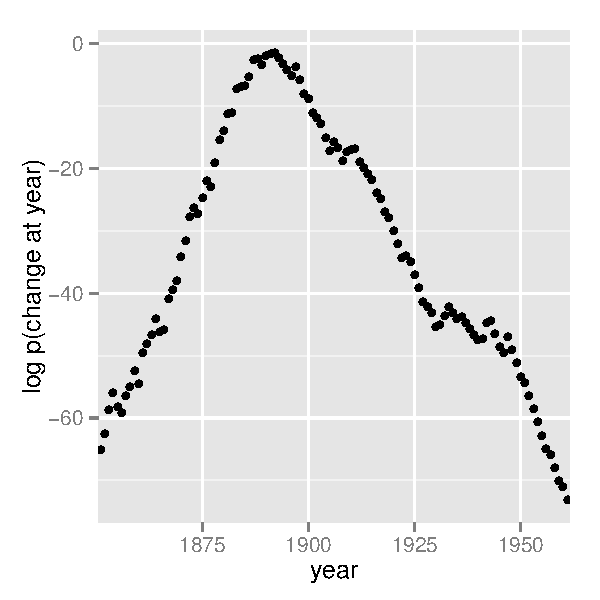
\includegraphics[height=2in]{img/change-point-posterior.pdf}
\ \ \ \ \
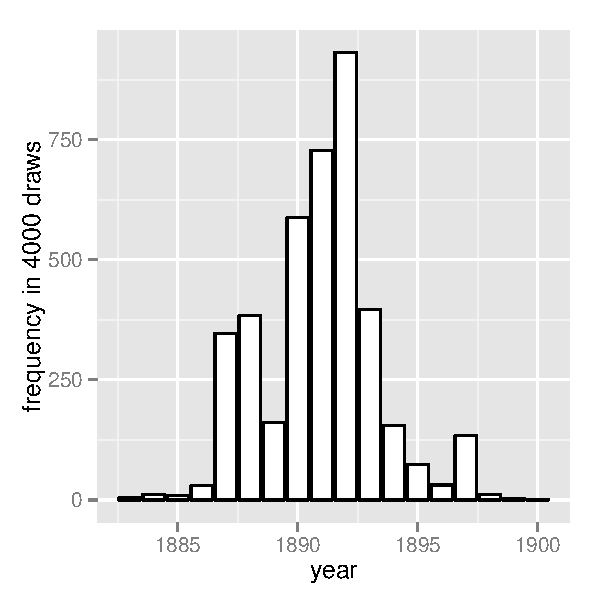
\includegraphics[height=2in]{img/s-discrete-posterior.pdf}
\end{center}
\vspace*{-12pt}
\caption{\small\it The posterior estimates for the change point.  \
  {\rm Left)} log probability of change point being in year,
  calculated analytically using \code{lp}; \ {\rm Right)}\ frequency
  of change point draws in the posterior generated using
  \code{lp}. The plot on the left is on the log scale and the plot on
  the right on the linear scale; note the narrower range of years in
  the right-hand plot resulting from sampling. The posterior mean of
  $s$ is roughly 1891.}%
\label{change-point-posterior.figure}
\end{figure}
%



\subsection{Discrete Sampling}

The generated quantities block may be used to draw discrete parameter
values using the built-in pseudo-random number generators.  For
example, with \code{lp} defined as above, the following program
draws a random value for \code{s} at every iteration.
%
\begin{stancode}
generated quantities {
  int<lower=1,upper=T> s;
  s = categorical_logit_rng(lp);
}
\end{stancode}
%
A posterior histogram of draws for $s$ is shown on the right side of
\reffigure{change-point-posterior}.

Compared to working in terms of expectations, discrete sampling is
highly inefficient, especially for tails of distributions, so this
approach should only be used if draws from a distribution are
explicitly required.   Otherwise, expectations should be computed in
the generated quantities block based on the posterior distribution for
\code{s} given by \code{softmax(lp)}.


\subsection{Posterior Covariance}

The discrete sample generated for $s$ can be used to calculate
covariance with other parameters.  Although the sampling approach is
straightforward, it is more statistically efficient (in the sense of
requiring far fewer iterations for the same degree of accuracy) to
calculate these covariances in expectation using \code{lp}.


\subsection{Multiple Change Points}

There is no obstacle in principle to allowing multiple change points.
The only issue is that computation increases from linear to quadratic
in marginalizing out two change points, cubic for three change points,
and so on.  There are three parameters, \code{e}, \code{m}, and
\code{l}, and two loops for the change point and then one over time,
with log densities being stored in a matrix.
%
\begin{stancode}
matrix[T, T] lp;
lp = rep_matrix(log_unif, T);
for (s1 in 1:T)
  for (s2 in 1:T)
    for (t in 1:T)
      lp[s1,s2] = lp[s1,s2]
        + poisson_lpmf(D[t] | t < s1 ? e : (t < s2 ? m : l));
\end{stancode}
%
The matrix can then be converted back to a vector using
\code{to\_vector} before being passed to \code{log\_sum\_exp}.

\section{Mark-Recapture Models}

A widely applied field method in ecology is to capture (or sight)
animals, mark them (e.g., by tagging), then release them.  This
process is then repeated one or more times, and is often done for
populations on an ongoing basis.  The resulting data may be used to
estimate population size.

The first subsection describes a very simple mark-recapture model that does
not involve any latent discrete parameters.  The following subsections
describes the Cormack-Jolly-Seber model, which involves latent
discrete parameters for animal death.

\subsection{Simple Mark-Recapture Model}

In the simplest case, a one-stage mark-recapture study produces the
following data
%
\begin{itemize}
\item $M$ : number of animals marked in first capture,
\item $C$ : number animals in second capture, and
\item $R$ : number of marked animals in second capture.
\end{itemize}
%
The estimand of interest is
%
\begin{itemize}
\item $N$ : number of animals in the population.
\end{itemize}
%
Despite the notation, the model will take $N$ to be a continuous
parameter; just because the population must be finite doesn't mean the
parameter representing it must be.  The parameter will be used to
produce a real-valued estimate of the population size.

The Lincoln-Petersen \citep{Lincoln:1930,Petersen:1896} method for
estimating population size is
%
\[
\hat{N} = \frac{M C}{R}.
\]
%
This population estimate would arise from a probabilistic model in
which the number of recaptured animals is distributed binomially,
\[
R \sim \distro{Binomial}(C, M / N)
\]
given the total number of animals captured in the second round ($C$)
with a recapture probability of $M/N$, the fraction of the total
population $N$ marked in the first round.

%
\begin{figure}
\begin{stancode}
data {
  int<lower=0> M;
  int<lower=0> C;
  int<lower=0,upper=min(M,C)> R;
}
parameters {
  real<lower=(C - R + M)> N;
}
model {
  R ~ binomial(C, M / N);
}
\end{stancode}
\vspace*{-6pt}
\caption{\small\it A probabilistic formulation of the Lincoln-Petersen
estimator for population size based on data from a one-step
mark-recapture study.  The lower bound on $N$ is necessary to
efficiently eliminate impossible values.}%
\label{lincoln-petersen-model.figure}
\end{figure}
%
The probabilistic variant of the Lincoln-Petersen estimator can be
directly coded in Stan as shown in \reffigure{lincoln-petersen-model}.
The Lincoln-Petersen estimate is the maximum likelihood estimate (MLE)
for this model.

To ensure the MLE is the Lincoln-Petersen estimate, an improper
uniform prior for $N$ is used; this could (and should) be replaced
with a more informative prior if possible based on knowledge of the
population under study.

The one tricky part of the model is the lower bound $C - R + M$ placed
on the population size $N$.  Values below this bound are impossible
because it is otherwise not possible to draw $R$ samples out of the
$C$ animals recaptured.  Implementing this lower bound is necessary to
ensure sampling and optimization can be carried out in an
unconstrained manner with unbounded support for parameters on the
transformed (unconstrained) space.  The lower bound in the declaration
for $C$ implies a variable transform
$f : (C-R+M,\infty) \rightarrow (-\infty,+\infty)$ defined by
$f(N) = \log(N - (C - R + M))$; the reference manual contains full
details of all constrained parameter transforms.

\subsection{Cormack-Jolly-Seber with Discrete Parameter}

The Cormack-Jolly-Seber (CJS) model
\citep{Cormack:1964,Jolly:1965,Seber:1965} is an open-population model
in which the population may change over time due to death; the
presentation here draws heavily on \citep{Schofield:2007}.

The basic data is
%
\begin{itemize}
\item $I$ : number of individuals,
\item $T$ : number of capture periods, and
\item $y_{i,t}$ : boolean indicating if individual $i$ was captured at
  time $t$.
\end{itemize}
%
Each individual is assumed to have been captured at least once because
an individual only contributes information conditionally after they
have been captured the first time.

There are two Bernoulli parameters in the model,
%
\begin{itemize}
\item $\phi_t$ : probability that animal alive at time $t$ survives
  until $t + 1$ and
\item $p_t$ : probability that animal alive at time $t$ is captured at
  time $t$.
\end{itemize}
%
These parameters will both be given uniform priors, but information
should be used to tighten these priors in practice.

The CJS model also employs a latent discrete parameter $z_{i,t}$
indicating for each individual $i$ whether it is alive at time $t$,
distributed as
%
\[
z_{i,t} \sim \distro{Bernoulli}(\ternary{z_{i,t-1}}{0}{\phi_{t-1}}).
\]
%
The conditional prevents the model positing zombies; once an animal is
dead, it stays dead.  The data distribution is then simple to express
conditional on $z$ as
%
\[
y_{i,t} \sim \distro{Bernoulli}(\ternary{z_{i,t}}{0}{p_t})
\]
%
The conditional enforces the constraint that dead animals cannot be captured.


\subsection{Collective Cormack-Jolly-Seber Model}

This subsection presents an implementation of the model in terms of
counts for different history profiles for individuals over three
capture times. It assumes exchangeability of the animals in that each
is assigned the same capture and survival probabilities.

In order to ease the marginalization of the latent discrete parameter
$z_{i,t}$, the Stan models rely on a derived quantity $\chi_t$ for
the probability that an individual is never captured again if it is
alive at time $t$ (if it is dead, the recapture probability is zero).
this quantity is defined recursively by
\[
\chi_t
=
\begin{cases}
1
& \mbox{if } t = T
\\[3pt]
(1 - \phi_t) + \phi_t (1 - p_{t+1}) \chi_{t+1}
& \mbox{ if } t < T
\end{cases}
\]
%
The base case arises because if an animal was captured in the last
time period, the probability it is never captured again is 1 because
there are no more capture periods.  The recursive case defining
$\chi_{t}$ in terms of $\chi_{t+1}$ involves two possibilities: (1)
not surviving to the next time period, with probability $(1 -
\phi_t)$, or (2) surviving to the next time period with probability
$\phi_t$, not being captured in the next time period with probability
$(1 - p_{t+1})$, and not being captured again after being alive in
period $t+1$ with probability $\chi_{t+1}$.

With three capture times, there are three captured/not-captured
profiles an individual may have.  These may be naturally coded as
binary numbers as follows.
%
\begin{center}
\begin{tabular}{c|ccc|c}
& \multicolumn{3}{|c|}{{\it captures}}
\\
{\it profile} & 1 & 2 & 3 & {\it probability}
\\ \hline
{0} & - & - & - & n/a
\\
{1} & - & - & + & n/a
\\ \hline
{2} & - & + & - & $\chi_2$
\\
{3} & - & + & + & $\phi_2 \, p_3$
\\ \hline
{4} & + & - & - & $\chi_1$
\\
{5} & + & - & + & $\phi_1 \, (1 - p_2) \, \phi_2 \, p_3$
\\ \hline
{6} & + & + & - & $ \phi_1 \, p_2 \, \chi_2$
\\
{7} & + & + & + & $\phi_1 \, p_2 \, \phi_2 \, p_3$
\end{tabular}
\end{center}
%
History 0, for animals that are never captured, is unobservable
because only animals that are captured are observed. History 1, for
animals that are only captured in the last round, provides no
information for the CJS model, because capture/non-capture status is
only informative when conditioned on earlier captures.  For the
remaining cases, the contribution to the likelihood is provided in the
final column.

By defining these probabilities in terms of $\chi$ directly, there is
no need for a latent binary parameter indicating whether an animal is
alive at time $t$ or not.  The definition of $\chi$ is typically used
to define the likelihood (i.e., marginalize out the latent discrete
parameter) for the CJS model \citep[page 9]{Schofield:2007}.

The Stan model defines $\chi$ as a transformed parameter based on
parameters $\phi$ and $p$.  In the model block, the log probability is
incremented for each history based on its count.  This second step is
similar to collecting Bernoulli observations into a binomial or
categorical observations into a multinomial, only it is coded directly
in the Stan program using \code{target~+=} rather than
being part of a built-in probability function.
%
\begin{figure}
\begin{stancode}
data {
  int<lower=0> history[7];
}
parameters {
  real<lower=0,upper=1> phi[2];
  real<lower=0,upper=1> p[3];
}
transformed parameters {
  real<lower=0,upper=1> chi[2];
  chi[2] = (1 - phi[2]) + phi[2] * (1 - p[3]);
  chi[1] = (1 - phi[1]) + phi[1] * (1 - p[2]) * chi[2];
}
model {
  target += history[2] * log(chi[2]);
  target += history[3] * (log(phi[2]) + log(p[3]));
  target += history[4] * (log(chi[1]));
  target += history[5] * (log(phi[1]) + log1m(p[2])
                            + log(phi[2]) + log(p[3]));
  target += history[6] * (log(phi[1]) + log(p[2])
                            + log(chi[2]));
  target += history[7] * (log(phi[1]) + log(p[2])
                            + log(phi[2]) + log(p[3]));
}
generated quantities {
  real<lower=0,upper=1> beta3;
  beta3 = phi[2] * p[3];
}
\end{stancode}
\vspace*{-12pt}
\caption{\small\it A Stan program for the Cormack-Jolly-Seber
  mark-recapture model that considers counts of individuals with
  observation histories of being observed or not in three capture
  periods.}\label{cjs-history.figure}
\end{figure}
%

\subsubsection{Identifiability}

The parameters $\phi_2$ and $p_3$, the probability of death at time 2
and probability of capture at time 3 are not identifiable, because both
may be used to account for lack of capture at time 3.  Their product,
$\beta_3 = \phi_2 \, p_3$, is identified.  The Stan model defines
\code{beta3} as a generated quantity.  Unidentified parameters pose a
problem for Stan's samplers' adaptation.  Although the problem posed
for adaptation is mild here because the parameters are bounded and
thus have proper uniform priors, it would be better to formulate an
identified parameterization.  One way to do this would be to formulate
a hierarchical model for the $p$ and $\phi$ parameters.

\subsection{Individual Cormack-Jolly-Seber Model}

This section presents a version of the Cormack-Jolly-Seber (CJS) model
cast at the individual level rather than collectively as in the
previous subsection.  It also extends the model to allow an arbitrary
number of time periods.  The data will consist of the number $T$ of
capture events, the number $I$ of individuals, and a boolean flag
$y_{i,t}$ indicating if individual $i$ was observed at time $t$.  In
Stan,
%
\begin{stancode}
data {
  int<lower=2> T;
  int<lower=0> I;
  int<lower=0,upper=1> y[I, T];
}
\end{stancode}

The advantages to the individual-level model is that it becomes
possible to add individual ``random effects'' that affect survival or
capture probability, as well as to avoid the combinatorics involved in
unfolding $2^T$ observation histories for $T$ capture times.

\subsubsection{Utility Functions}

The individual CJS model is written involves several function
definitions.  The first two are used in the transformed data block to
compute the first and last time period in which an animal was
captured.%
%
\footnote{An alternative would be to compute this on the outside and
feed it into the Stan model as preprocessed data.  Yet another
alternative encoding would be a sparse one recording only the
capture events along with their time and identifying the individual
captured.}
%
\begin{stancode}
functions {
  int first_capture(int[] y_i) {
    for (k in 1:size(y_i))
      if (y_i[k])
        return k;
    return 0;
  }
  int last_capture(int[] y_i) {
    for (k_rev in 0:(size(y_i) - 1)) {
      int k;
      k = size(y_i) - k_rev;
      if (y_i[k])
        return k;
    }
    return 0;
  }
  ...
}
\end{stancode}
%
These two functions are used to define the first and last capture time
for each individual in the transformed data block.%
%
\footnote{Both functions return 0 if the individual represented by the
  input array was never captured.  Individuals with no captures are
  not relevant for estimating the model because all probability
  statements are conditional on earlier captures.  Typically they
  would be removed from the data, but the program allows them to be
  included even though they make not contribution to the log
  probability function.}
%
\begin{stancode}
transformed data {
  int<lower=0,upper=T> first[I];
  int<lower=0,upper=T> last[I];
  vector<lower=0,upper=I>[T] n_captured;
  for (i in 1:I)
    first[i] = first_capture(y[i]);
  for (i in 1:I)
    last[i] = last_capture(y[i]);
  n_captured = rep_vector(0, T);
  for (t in 1:T)
    for (i in 1:I)
      if (y[i, t])
        n_captured[t] = n_captured[t] + 1;
}
\end{stancode}
%
The transformed data block also defines \code{n\_captured[t]}, which is
the total number of captures at time \code{t}.  The variable
\code{n\_captured} is defined as a vector instead of an integer array
so that it can be used in an elementwise vector operation in the generated
quantities block to model the population estimates at each time point.

The parameters and transformed parameters are as before, but now there
is a function definition for computing the entire vector \code{chi}, the
probability that if an individual is alive at \code{t} that it will
never be captured again.
%
\begin{stancode}
parameters {
  vector<lower=0,upper=1>[T-1] phi;
  vector<lower=0,upper=1>[T] p;
}
transformed parameters {
  vector<lower=0,upper=1>[T] chi;
  chi = prob_uncaptured(T,p,phi);
}
\end{stancode}
%
The definition of \code{prob\_uncaptured}, from the functions block,
is
%
\begin{stancode}
functions {
  ...
  vector prob_uncaptured(int T, vector p, vector phi) {
    vector[T] chi;
    chi[T] = 1.0;
    for (t in 1:(T - 1)) {
      int t_curr;
      int t_next;
      t_curr = T - t;
      t_next = t_curr + 1;
      chi[t_curr] = (1 - phi[t_curr])
                     + phi[t_curr]
                       * (1 - p[t_next])
                       * chi[t_next];
    }
    return chi;
  }
}
\end{stancode}
%
The function definition directly follows the mathematical definition
of $\chi_t$, unrolling the recursion into an iteration and
defining the elements of \code{chi} from \code{T} down to 1.

\subsubsection{The Model}

Given the precomputed quantities, the model block directly encodes the
CJS model's log likelihood function.  All parameters are left with
their default uniform priors and the model simply encodes the log
probability of the observations \code{q} given the parameters \code{p}
and \code{phi} as well as the transformed parameter \code{chi} defined
in terms of \code{p} and \code{phi}.
%
\begin{stancode}
model {
  for (i in 1:I) {
    if (first[i] > 0) {
      for (t in (first[i]+1):last[i]) {
        1 ~ bernoulli(phi[t-1]);
        y[i, t] ~ bernoulli(p[t]);
      }
      1 ~ bernoulli(chi[last[i]]);
    }
  }
}
\end{stancode}
%
The outer loop is over individuals, conditional skipping individuals
\code{i} which are never captured.  The never-captured check depends
on the convention of the first-capture and last-capture functions
returning 0 for \code{first} if an individual is never captured.

The inner loop for individual \code{i} first increments the log
probability based on the survival of the individual with probability
\code{phi[t-1]}.  The outcome of 1 is fixed because the individual
must survive between the first and last capture (i.e., no zombies).
Note that the loop starts after the first capture, because all
information in the CJS model is conditional on the first capture.

In the inner loop, the observed capture status \code{y[i,~t]} for
individual \code{i} at time \code{t} has a Bernoulli distribution
based on the capture probability \code{p[t]} at time \code{t}.

After the inner loop, the probability of an animal never being seen
again after being observed at time \code{last[i]} is included, because
\code{last[i]} was defined to be the last time period in which animal
\code{i} was observed.

\subsubsection{Identified Parameters}

As with the collective model described in the previous subsection,
this model does not identify \code{phi[T-1]} and \code{p[T]}, but
does identify their product, \code{beta}.  Thus \code{beta} is defined
as a generated quantity to monitor convergence and report.
%
\begin{stancode}
generated quantities {
  real beta;
  ...

  beta = phi[T-1] * p[T];
  ...
}
\end{stancode}
%

The parameter \code{p[1]} is also not modeled and will just be uniform
between 0 and 1.  A more finely articulated model might have a
hierarchical or time-series component, in which case \code{p[1]} would
be an unknown initial condition and both \code{phi[T-1]} and
\code{p[T]} could be identified.

\subsubsection{Population Size Estimates}

The generated quantities also calculates an estimate of the population
mean at each time \code{t} in the same way as in the simple
mark-recapture model as the number of individuals captured at time
\code{t} divided by the probability of capture at time \code{t}.  This
is done with the elementwise division operation for vectors
(\code{./}) in the generated quantities block.
%
\begin{stancode}
generated quantities {
  ...
  vector<lower=0>[T] pop;
  ...
  pop = n_captured ./ p;
  pop[1] = -1;
}
\end{stancode}

\subsubsection{Generalizing to Individual Effects}

All individuals are modeled as having the same capture probability,
but this model could be easily generalized to use a logistic
regression here based on individual-level inputs to be used as
predictors.



\section{Data Coding and Diagnostic Accuracy Models}

Although seemingly disparate tasks, the rating/coding/annotation of
items with categories and diagnostic testing for disease or other
conditions share several characteristics which allow their statistical
properties to modeled similarly.

\subsection{Diagnostic Accuracy}

Suppose you have diagnostic tests for a condition of varying
sensitivity and specificity.  Sensitivity is the probability a test
returns positive when the patient has the condition and specificity is
the probability that a test returns negative when the patient does not
have the condition.  For example, mammograms and puncture biopsy tests
both test for the presence of breast cancer.  Mammograms have high
sensitivity and low specificity, meaning lots of false positives,
whereas puncture biopsies are the opposite, with low sensitivity and
high specificity, meaning lots of false negatives.

There are several estimands of interest in such studies.  An
epidemiological study may be interested in the prevalence of a kind of
infection, such as malaria, in a population.  A test development study
might be interested in the diagnostic accuracy of a new test. A health
care worker performing tests might be interested in the disease status
of a particular patient.

\subsection{Data Coding}

Humans are often given the task of coding (equivalently rating or
annotating) data.  For example, journal or grant reviewers rate
submissions, a political study may code campaign commercials as to
whether they are attack ads or not, a natural language processing
study might annotate Tweets as to whether they are positive or
negative in overall sentiment, or a dentist looking at an X-ray
classifies a patient as having a cavity or not.  In all of these
cases, the data coders play the role of the diagnostic tests and all
of the same estimands are in play --- data coder accuracy and bias,
true categories of items being coded, or the prevalence of various
categories of items in the data.

\subsection{Noisy Categorical Measurement Model}

In this section, only categorical ratings are considered, and the
challenge in the modeling for Stan is to marginalize out the discrete
parameters.

\cite{DawidSkene:1979} introduce a noisy-measurement model for
data coding and apply in the epidemiological setting of coding what
doctor notes say about patient histories;  the same model can be used
for diagnostic procedures.

\subsubsection{Data}

The data for the model consists of $J$ raters (diagnostic tests), $I$
items (patients), and $K$ categories (condition statuses) to annotate,
with $y_{i, j} \in 1{:}K$ being the rating provided by rater $j$ for
item $i$.  In a diagnostic test setting for a particular condition,
the raters are diagnostic procedures and often $K=2$, with values
signaling the presence or absence of the condition.%
%
\footnote{Diagnostic procedures are often ordinal, as in stages of
  cancer in oncological diagnosis or the severity of a cavity in
  dental diagnosis.  Dawid and Skene's model may be used as is or
  naturally generalized for ordinal ratings using a latent continuous
  rating and cutpoints as in ordinal logistic regression.}

It is relatively straightforward to extend Dawid and Skene's model to
deal with the situation where not every rater rates each item exactly
once.

\subsection{Model Parameters}

The model is based on three parameters, the first of which is discrete:
%
\begin{itemize}
\item $z_i$ : a value in $1{:}K$ indicating the true category of item $i$,
\item $\pi$ : a $K$-simplex for the prevalence of the $K$
  categories in the population, and
\item $\theta_{j,k}$ : a $K$-simplex for the response of annotator $j$
  to an item of true category $k$.
\end{itemize}

\subsection{Noisy Measurement Model}

The true category of an item is assumed to be generated by a simple
categorical distribution based on item prevalence,
\[
z_i \sim \distro{Categorical}(\pi).
\]
%
The rating $y_{i, j}$ provided for item $i$ by rater $j$ is modeled as
a categorical response of rater $i$ to an item of category $z_i$,%
%
\footnote{In the subscript, $z[i]$ is written as $z_i$ to
  improve legibility.}
%
\[
y_{i, j} \sim \distro{Categorical}(\theta_{j,\pi_{z[i]}}).
\]

\subsubsection{Priors and Hierarchical Modeling}

Dawid and Skene provided maximum likelihood estimates for $\theta$ and
$\pi$, which allows them to generate probability estimates for each $z_i$.

To mimic Dawid and Skene's maximum likelihood model, the parameters
$\theta_{j,k}$ and $\pi$ can be given uniform priors over
$K$-simplexes.  It is straightforward to generalize to Dirichlet
priors,
\[
\pi \sim \distro{Dirichlet}(\alpha)
\]
and
\[
\theta_{j,k} \sim \distro{Dirichlet}(\beta_k)
\]
with fixed hyperparameters $\alpha$ (a vector) and $\beta$ (a matrix
or array of vectors).  The prior for $\theta_{j,k}$ must be allowed to
vary in $k$, so that, for instance, $\beta_{k,k}$ is large enough to
allow the prior to favor better-than-chance annotators over random or
adversarial ones.

Because there are $J$ coders, it would be natural to extend the model
to include a hierarchical prior for $\beta$ and to partially pool the
estimates of coder accuracy and bias.

\subsubsection{Marginalizing out the True Category}

Because the true category parameter $z$ is discrete, it must be
marginalized out of the joint posterior in order to carry out sampling
or maximum likelihood estimation in Stan. The joint posterior factors
as
\[
p(y, \theta, \pi) = p(y | \theta,\pi) \, p(\pi) \, p(\theta),
\]
where $p(y | \theta,\pi)$ is derived by marginalizing $z$ out of
%
\[
p(z, y | \theta, \pi)
\ = \
\prod_{i=1}^I \left( \distro{Categorical}(z_i | \pi)
                     \prod_{j=1}^J
                     \distro{Categorical}(y_{i, j}|\theta_{j, z[i]})
              \right).
\]
%
This can be done item by item, with
\[
p(y | \theta, \pi)
\ = \
\prod_{i=1}^I \sum_{k=1}^K
  \left( \distro{Categorical}(z_i | \pi)
         \prod_{j=1}^J
         \distro{Categorical}(y_{i, j}|\theta_{j, z[i]})
  \right).
\]
%
In the missing data model, only the observed labels would be used in
the inner product.

\cite{DawidSkene:1979} derive exactly the same equation in their
Equation~(2.7), required for the E-step in their expectation
maximization (EM) algorithm.  Stan requires the marginalized
probability function on the log scale,
\[
\begin{array}{l}
\mbox{ } \ \log p(y | \theta, \pi)
\\[3pt]
\mbox{ } \  = \
\sum_{i=1}^I \log \left( \sum_{k=1}^K \exp
  \left( \log \distro{Categorical}(z_i | \pi)
         + \sum_{j=1}^J
         \log \distro{Categorical}(y_{i, j}|\theta_{j, z[i]})
  \right) \right),
\end{array}
\]
which can be directly coded using Stan's built-in \code{log\_sum\_exp}
function.


\subsection{Stan Implementation}

The Stan program for the Dawid and Skene model is provided in
\reffigure{dawid-skene-model}.
%
\begin{figure}
\begin{stancode}
data {
  int<lower=2> K;
  int<lower=1> I;
  int<lower=1> J;

  int<lower=1,upper=K> y[I, J];

  vector<lower=0>[K] alpha;
  vector<lower=0>[K] beta[K];
}
parameters {
  simplex[K] pi;
  simplex[K] theta[J, K];
}
transformed parameters {
  vector[K] log_q_z[I];
  for (i in 1:I) {
    log_q_z[i] = log(pi);
    for (j in 1:J)
      for (k in 1:K)
        log_q_z[i, k] = log_q_z[i, k]
                         + log(theta[j, k, y[i, j]]);
  }
}
model {
  pi ~ dirichlet(alpha);
  for (j in 1:J)
    for (k in 1:K)
      theta[j, k] ~ dirichlet(beta[k]);

  for (i in 1:I)
    target += log_sum_exp(log_q_z[i]);
}
\end{stancode}
\vspace*{-12pt}
\caption{\small\it Stan program for the rating (or diagnostic
  accuracy) model of \cite{DawidSkene:1979}. The model marginalizes
  out the discrete parameter $z$, storing the unnormalized conditional
  probability $\log q(z_i=k|\theta,\pi)$ in\ \code{log\_q\_z[i,~k]}.}%
\label{dawid-skene-model.figure}
\end{figure}
%
The Stan model converges quickly and mixes well using NUTS starting at
diffuse initial points, unlike the equivalent model implemented with
Gibbs sampling over the discrete parameter.  Reasonable weakly
informative priors are $\alpha_k = 3$ and $\beta_{k,k} = 2.5 K$ and
$\beta_{k,k'} = 1$ if $k \neq k'$.  Taking $\alpha$ and $\beta_k$ to
be unit vectors and applying optimization will produce the same answer
as the expectation maximization (EM) algorithm of
\cite{DawidSkene:1979}.

\subsubsection{Inference for the True Category}

The quantity \code{log\_q\_z[i]} is defined as a transformed
parameter.  It encodes the (unnormalized) log of $p(z_i | \theta,
\pi)$.  Each iteration provides a value conditioned on that
iteration's values for $\theta$ and $\pi$.  Applying the softmax
function to \code{log\_q\_z[i]} provides a simplex corresponding to
the probability mass function of $z_i$ in the posterior.   These may
be averaged across the iterations to provide the posterior probability
distribution over each $z_i$.


\chapter{Sparse and Ragged Data Structures}\label{sparse-ragged.chapter}

\noindent
Stan does not directly support either sparse or ragged data
structures, though both can be accommodated with some programming
effort.  \refchapter{sparse-matrices} introduces a special-purpose
sparse matrix times dense vector multiplication, which should be used
where applicable;  this chapter covers more general data structures.

\section{Sparse Data Structures}

Coding sparse data structures is as easy as moving from a matrix-like
data structure to a database-like data structure.  For example,
consider the coding of sparse data for the IRT models discussed in
\refsection{item-response-models}.  There are $J$ students and $K$
questions, and if every student answers every question, then it is
practical to declare the data as a $J \times K$ array of answers.
%
\begin{quote}
\begin{Verbatim}
data {
  int<lower=1> J;
  int<lower=1> K;
  int<lower=0,upper=1> y[J, K];
  ...
model {
  for (j in 1:J)
    for (k in 1:K)
      y[j, k] ~ bernoulli_logit(delta[k] * (alpha[j] - beta[k]));
  ...
\end{Verbatim}
\end{quote}
%

\begin{figure}
\begin{center}
\begin{minipage}[c]{0.45\textwidth}
\[
y
=
\left[
\begin{array}{cccc}
0 & 1 & \mbox{NA} & 1
\\
0 & \mbox{NA} & \mbox{NA} & 1
\\
\mbox{NA} & 0 & \mbox{NA} & \mbox{NA}
\end{array}
\right]
\]
\end{minipage}
\ \ \
\begin{minipage}[c]{0.45\textwidth}
\begin{tabular}{ll|l}
$jj$ & $kk$ & $y$
\\ \hline
1 & 1 & 0
\\
1 & 2 & 1
\\
1 & 4 & 1
\\
2 & 1 & 0
\\
2 & 4 & 1
\\
3 & 2 & 0
\end{tabular}
\end{minipage}
\end{center}
\vspace*{-12pt}
\caption{\small\it  Example of coding sparse arrays in Stan.  On the left is a definition
  of a sparse matrix $y$ using the NA notation from R (which is not
  supported by Stan).  On the right is a database-like encoding of the
  same sparse matrix $y$ that can be used directly in Stan.  The first
  two columns, $jj$ and $kk$, denote the indexes and the final column,
  $y$, the value.  For example, the fifth row of the database-like
  data structure on the right indicates that $y_{2,4} = 1$.}\label{sparse-data.figure}
\end{figure}
%
When not every student is given every question, the dense array coding
will no longer work, because Stan does not support undefined values.
\reffigure{sparse-data} shows an example with $J=3$ and $K=4$, with
missing responses shown as NA, as in R.  There is no support within
Stan for R's NA values, so this data structure cannot be used
directly.  Instead, it must be converted to a ``long form'' as in a
database, with columns indicating the $j$ and $k$ indexes along with
the value.  For instance, with $jj$ and $kk$ used for the indexes
(following \citep{GelmanHill:2007}), the data structure can be coded
as in the right-hand example in \reffigure{sparse-data}.  This says
that $y_{1,1} = 0$, $y_{1,2} = 1$, and so on, up to $y_{3,2} = 1$,
with all other entries undefined.

Letting $N$ be the number of $y$ that are defined, here $N=6$,
the data and model can be formulated as follows.
%
\begin{quote}
\begin{Verbatim}
data {
  ...
  int<lower=1> N;
  int<lower=1,upper=J> jj[N];
  int<lower=1,upper=K> kk[N];
  int<lower=0,upper=1> y[N];
  ...
model {
  for (n in 1:N)
    y[n] ~ bernoulli_logit(delta[kk[n]]
                           * (alpha[jj[n]] - beta[kk[n]]));
  ...
\end{Verbatim}
\end{quote}
%
In the situation where there are no missing values, the two model
formulations produce exactly the same log posterior density.


\section{Ragged Data Structures}\label{ragged-data-structs.section}

Ragged arrays are arrays that are not rectangular, but have different
sized entries.  This kind of structure crops up when there are
different numbers of observations per entry.

A general approach to dealing with ragged structure is to move to a
full database-like data structure as discussed in the previous
section.  A more compact approach is possible with some indexing into
a linear array.

For example, consider a data structure for three groups, each of which
has a different number of observations.
%
\begin{figure}
\begin{center}
\begin{minipage}[c]{0.35\textwidth}
$y_1 =  \left[1.3 \ \ 2.4 \ \ 0.9\right]$
\\[3pt]
$y_2 = \left[-1.8 \ \ -0.1\right]$
\\[3pt]
$y_3 = \left[12.9 \ \ 18.7 \ \ 42.9 \ \ 4.7\right]$
\end{minipage}
\ \ \
\begin{minipage}[c]{0.60\textwidth}
$z = [1.3 \ \ 2.4 \ \ 0.9 \ \ -1.8 \ \ -0.1 \ \ 12.9 \ \ 18.7 \ \ 42.9
\ \ 4.7]$
\\[3pt]
$s  =  \{ 3 \ \ 2 \ \ 4 \}$
\end{minipage}
\end{center}
\caption{\small\it Example of coding ragged arrays in Stan.  On the
  left is the definition of a ragged data structure $y$ with three
  rows of different sizes ($y_1$ is size 3, $y_2$ size 2, and $y_3$
  size 4).  On the right is an example of how to code the data in Stan,
  using a single vector $y$ to hold all the values and a separate
  array of integers $s$ to hold the group row sizes.  In this
  example, $y_1 = z_{1:3}$, $y_2 =
  z_{4:5}$, and $y_3 = z_{6:9}$.}\label{ragged-data.figure}
\end{figure}
%

Suppose the model is a very simple varying intercept model, which,
using vectorized notation, would yield a likelihood
\[
\prod_{n=1}^3 \log \distro{Normal}(y_n | \mu_n, \sigma).
\]
There's no direct way to encode this in Stan.

A full database type structure could be used, as in the sparse
example, but this is inefficient, wasting space for unnecessary
indices and not allowing vector-based density operations.  A better
way to code this data is as a single list of values, with a separate
data structure indicating the sizes of each subarray.  This is
indicated on the right of \reffigure{ragged-data}.  This coding uses a
single array for the values and a separate array for the sizes of each
row.

The model can then be coded up using slicing operations as follows.
\begin{quote}
\begin{Verbatim}
data {
  int<lower=0> N;   // # observations
  int<lower=0> K;   // # of groups
  vector[N] y;      // observations
  int s[K];         // group sizes
  ...
model {
  int pos;
  pos = 1;
  for (k in 1:K) {
    segment(y, pos, s[k]) ~ normal(mu[k], sigma);
    pos = pos + s[k];
  }
\end{Verbatim}
\end{quote}
%
This coding allows for efficient vectorization, which is worth the
copy cost entailed by the \code{segment()} vector slicing operation.


\chapter{Clustering Models}\label{clustering.chapter}

\noindent
Unsupervised methods for organizing data into groups are collectively
referred to as clustering.  This chapter describes the implementation
in Stan of two widely used statistical clustering models, soft
$K$-means and latent Dirichlet allocation (LDA).  In addition, this
chapter includes naive Bayesian classification, which can be viewed as
a form of clustering which may be supervised.  These models are
typically expressed using discrete parameters for cluster assignments.
Nevertheless, they can be implemented in Stan like any other mixture
model by marginalizing out the discrete parameters (see
\refchapter{mixture-modeling}).

\section{Relation to Finite Mixture Models}

As mentioned in \refsection{clustering-mixture}, clustering models and
finite mixture models are really just two sides of the same coin.  The
``soft'' $K$-means model described in the next section is a normal
mixture model (with varying assumptions about covariance in higher
dimensions leading to variants of $K$-means).  Latent Dirichlet
allocation is a mixed-membership multinomial mixture.

\section{Soft $K$-Means}

$K$-means clustering is a method of clustering data represented as
$D$-dimensional vectors.  Specifically, there will be $N$ items to be
clustered, each represented as a vector $y_n \in \reals^D$.  In the
``soft'' version of $K$-means, the assignments to clusters will be
probabilistic.

\subsection{Geometric Hard  $K$-Means Clustering}

$K$-means clustering is typically described geometrically in terms of
the following algorithm, which assumes the number of clusters $K$ and
data vectors $y$ as input.
%
\begin{enumerate}
\item For each $n$ in $1:N$, randomly assign vector $y_n$ to a cluster in $1{:}K$;
\item Repeat
\begin{enumerate}
\item For each cluster $k$ in $1{:}K$, compute the cluster centroid $\mu_k$  by averaging the
  vectors assigned to that cluster;
\item For each $n$ in $1:N$, reassign $y_n$ to the cluster $k$
  for which the (Euclidean) distance from $y_n$ to $\mu_k$ is smallest;
\item If no vectors changed cluster, return the cluster assignments.
\end{enumerate}
\end{enumerate}
%
This algorithm is guaranteed to terminate.

\subsection{Soft $K$-Means Clustering}

Soft $K$-means clustering treats the cluster assignments as
probability distributions over the clusters.  Because of the
connection between Euclidean distance and multivariate normal models
with a fixed covariance, soft $K$-means can be expressed (and coded in
Stan) as a multivariate normal mixture model.

In the full generative model, each data point $n$ in $1{:}N$ is assigned
a cluster $z_n \in 1{:}K$ with symmetric uniform probability,
%
\[
z_n \sim \distro{Categorical}({\bf 1}/K),
\]
where ${\bf 1}$ is the unit vector of $K$ dimensions, so that ${\bf
  1}/K$ is the symmetric $K$-simplex.  Thus the model assumes that
each data point is drawn from a hard decision about cluster
membership.  The softness arises only from the uncertainty about which
cluster generated a data point.

The data points themselves are generated from a multivariate normal
distribution whose parameters are determined by the cluster assignment
$z_n$,
\[
y_n \sim  \distro{Normal}(\mu_{z[n]},\Sigma_{z[n]})
\]

The sample implementation in this section assumes a fixed unit
covariance matrix shared by all clusters $k$,
\[
\Sigma_k = \mbox{diag\_matrix}({\bf 1}),
\]
so that the log multivariate normal can be implemented directly up to a proportion
by
\[
\mbox{Normal}\left( y_n | \mu_k, \mbox{diag\_matrix}({\bf 1}) \right)
\propto \exp \left (- \frac{1}{2} \sum_{d=1}^D \left( \mu_{k,d} - y_{n,d}
  \right)^2 \right).
\]
The spatial perspective on $K$-means arises by noting that the inner
term is just half the negative Euclidean distance from the cluster
mean $\mu_k$ to the data point $y_n$.

\subsection{Stan Implementation of Soft $K$-Means}

Consider the following Stan program for implementing $K$-means
clustering.%
%
\footnote{The model is available in the Stan example model repository;
see \url{http://mc-stan.org/users/documentation}.}
%
\begin{stancode}
data {
  int<lower=0> N;  // number of data points
  int<lower=1> D;  // number of dimensions
  int<lower=1> K;  // number of clusters
  vector[D] y[N];  // observations
}
transformed data {
  real<upper=0> neg_log_K;
  neg_log_K = -log(K);
}
parameters {
  vector[D] mu[K]; // cluster means
}
transformed parameters {
  real<upper=0> soft_z[N, K]; // log unnormalized clusters
  for (n in 1:N)
    for (k in 1:K)
      soft_z[n, k] = neg_log_K
                     - 0.5 * dot_self(mu[k] - y[n]);
}
model {
  // prior
  for (k in 1:K)
    mu[k] ~ std_normal();

  // likelihood
  for (n in 1:N)
    target += log_sum_exp(soft_z[n]));
}
\end{stancode}
%
There is an independent standard normal prior on the centroid parameters;
this prior could be swapped with other priors, or even a hierarchical
model to fit an overall problem scale and location.

The only parameter is \code{mu}, where \code{mu[k]} is the centroid
for cluster $k$.  The transformed parameters \code{soft\_z[n]} contain
the log of the unnormalized cluster assignment probabilities.  The
vector \code{soft\_z[n]} can be converted back to a normalized simplex
using the softmax function (see \refsection{softmax}), either
externally or within the model's generated quantities block.

\subsection{Generalizing Soft $K$-Means}

The multivariate normal distribution with unit covariance matrix
produces a log probability density proportional to Euclidean distance
(i.e., $L_2$ distance).  Other distributions relate to other
geometries.  For instance, replacing the normal distribution with the
double exponential (Laplace) distribution produces a clustering model
based on $L_1$ distance (i.e., Manhattan or taxicab
distance).

Within the multivariate normal version of $K$-means, replacing the
unit covariance matrix with a shared covariance matrix amounts to
working with distances defined in a space transformed by the inverse
covariance matrix.

Although there is no global spatial analog, it is common to see soft
$K$-means specified with a per-cluster covariance matrix. In this
situation, a hierarchical prior may be used for the covariance matrices.



\section{The Difficulty of Bayesian Inference for Clustering}

Two problems make it pretty much impossible to perform full Bayesian
inference for clustering models, the lack of parameter identifiability
and the extreme multimodality of the posteriors.  There is additional
discussion related to the non-identifiability due to label switching
in \refsection{label-switching-problematic}.

\subsection{Non-Identifiability}

Cluster assignments are not identified --- permuting the cluster mean
vectors \code{mu} leads to a model with identical likelihoods.  For
instance, permuting the first two indexes in \code{mu} and the first
two indexes in each \code{soft\_z[n]} leads to an identical likelihood
(and prior).

The lack of identifiability means that the cluster parameters
cannot be compared across multiple Markov chains.  In fact, the only
parameter in soft $K$-means is not identified, leading to problems in
monitoring convergence.  Clusters can even fail to be identified
within a single chain, with indices swapping if the chain is long
enough or the data is not cleanly separated.

\subsection{Multimodality}

The other problem with clustering models is that their posteriors are
highly multimodal.  One form of multimodality is the
non-identifiability leading to index swapping.  But even without
the index problems the posteriors are highly multimodal.

Bayesian inference fails in cases of high multimodality because there
is no way to visit all of the modes in the posterior in appropriate
proportions and thus no way to evaluate integrals involved in
posterior predictive inference.

In light of these two problems, the advice often given in fitting
clustering models is to try many different initializations and select
the sample with the highest overall probability.  It is also popular
to use optimization-based point estimators such as expectation
maximization or variational Bayes, which can be much more efficient
than sampling-based approaches.


\section{Naive Bayes Classification and Clustering}

Naive Bayes is a kind of mixture model that can be used for
classification or for clustering (or a mix of both), depending on
which labels for items are observed.%
%
\footnote{For clustering, the non-identifiability problems for all
  mixture models present a problem, whereas there is no such problem
  for classification.  Despite the difficulties with full Bayesian
  inference for clustering, researchers continue to use it, often in
  an exploratory data analysis setting rather than for predictive
  modeling.}

Multinomial mixture models are referred to as ``naive Bayes'' because
they are often applied to classification problems where the
multinomial independence assumptions are clearly false.

Naive Bayes classification and clustering can be applied to any data
with multinomial structure.  A typical example of this is natural
language text classification and clustering, which is used an example
in what follows.

The observed data consists of a sequence of $M$ documents made up of
bags of words drawn from a vocabulary of $V$ distinct words.  A
document $m$ has $N_m$ words, which are indexed as $w_{m,1}, \ldots,
w_{m,N[m]} \in 1{:}V$.  Despite the ordered indexing of words in a
document, this order is not part of the model, which is clearly
defective for natural human language data.  A number of topics (or
categories) $K$ is fixed.

The multinomial mixture model generates a single category $z_m \in
1{:}K$ for each document $m \in 1{:}M$ according to a categorical
distribution,
\[
z_m \sim \distro{Categorical}(\theta).
\]
The $K$-simplex parameter $\theta$ represents the prevalence of each
category in the data.

Next, the words in each document are generated conditionally
independently of each other and the words in other documents based on
the category of the document, with word $n$ of document $m$ being
generated as
\[
w_{m,n} \sim \distro{Categorical}(\phi_{z[m]}).
\]
The parameter $\phi_{z[m]}$ is a $V$-simplex representing the
probability of each word in the vocabulary in documents of category
$z_m$.

The parameters $\theta$ and $\phi$ are typically given symmetric
Dirichlet priors.  The prevalence $\theta$ is sometimes fixed to
produce equal probabilities for each category $k \in 1:K$.

\subsection{Coding Ragged Arrays}

The specification for naive Bayes in the previous sections have used a ragged
array notation for the words $w$.  Because Stan does not support
ragged arrays, the models are coded using an alternative strategy that
provides an index for each word in a global list of words.   The data
is organized as follows, with the word arrays laid out in a column and each
assigned to its document in a second column.
%
\begin{center}
\begin{tabular}{r|cc}
\code{n} & \code{w[n]} & \code{doc[n]} \\ \hline
1 & $w_{1,1}$ & 1 \\
2 & $w_{1,2}$ & 1 \\
\vdots & \vdots & \vdots \\
$N_1$ & $w_{1,N[1]}$ & 1 \\
$N_1 + 1$ & $w_{2,1}$ & 2 \\
$N_1 + 2$ & $w_{2,2}$ & 2 \\
\vdots & \vdots & \vdots \\
$N_1 + N_2$ & $w_{2,N[2]}$ & 2 \\
$N_1 + N_2 + 1$ & $w_{3,1}$ & 3 \\
\vdots & \vdots & \vdots \\
$\code{N} = \sum_{m=1}^M N_m$ & $w_{M,N[M]}$ & $M$ \\
\end{tabular}
\end{center}
%
The relevant variables for the program are \code{N}, the total number
of words in all the documents, the word array \code{w}, and the
document identity array \code{doc}.

\subsection{Estimation with Category-Labeled Training Data}


A naive Bayes model for estimating the simplex parameters given
training data with documents of known categories can be coded in Stan
as follows%
%
\footnote{This model is available in the example model repository;
  see \url{http://mc-stan.org/users/documentation}.}
%
\begin{stancode}
data {
  // training data
  int<lower=1> K;               // num topics
  int<lower=1> V;               // num words
  int<lower=0> M;               // num docs
  int<lower=0> N;               // total word instances
  int<lower=1,upper=K> z[M];    // topic for doc m
  int<lower=1,upper=V> w[N];    // word n
  int<lower=1,upper=M> doc[N];  // doc ID for word n
  // hyperparameters
  vector<lower=0>[K] alpha;     // topic prior
  vector<lower=0>[V] beta;      // word prior
}
parameters {
  simplex[K] theta;   // topic prevalence
  simplex[V] phi[K];  // word dist for topic k
}
model {
  theta ~ dirichlet(alpha);
  for (k in 1:K)
    phi[k] ~ dirichlet(beta);
  for (m in 1:M)
    z[m] ~ categorical(theta);
  for (n in 1:N)
    w[n] ~ categorical(phi[z[doc[n]]]);
}
\end{stancode}
%
Note that the topic identifiers $z_m$ are declared as data and the
latent category assignments are included as part of the likelihood
function.

\subsection{Estimation without Category-Labeled Training Data}

Naive Bayes models can be used in an unsupervised fashion to cluster
multinomial-structured data into a fixed number $K$ of categories.
The data declaration includes the same variables as the model in the
previous section excluding the topic labels \code{z}.   Because
\code{z} is discrete, it needs to be summed out of the model
calculation.  This is done for naive Bayes as for other mixture
models.  The parameters are the same up to the priors, but the
likelihood is now computed as the marginal document probability
\[
\begin{array}{l}
\log p(w_{m,1},\ldots,w_{m,N_m}|\theta,\phi)
\\[2pt]
\ \ \ = \
\log \sum_{k=1}^K
\left( \distro{Categorical}(k|\theta)
        \times \prod_{n=1}^{N_m} \distro{Categorical}(w_{m,n}|\phi_k)
\right)
\\[6pt]
\ \ \ = \
\log \sum_{k=1}^K \exp \left(
\log \distro{Categorical}(k|\theta)
+ \sum_{n=1}^{N_m} \log \distro{Categorical}(w_{m,n}|\phi_k)
\right).
\end{array}
\]
%
The last step shows how the \code{log\_sum\_exp} function can be used
to stabilize the numerical calculation and return a result on the log
scale.
%
\begin{stancode}
model {
  real gamma[M, K];
  theta ~ dirichlet(alpha);
  for (k in 1:K)
    phi[k] ~ dirichlet(beta);
  for (m in 1:M)
    for (k in 1:K)
      gamma[m, k] = categorical_lpmf(k | theta);
  for (n in 1:N)
    for (k in 1:K)
      gamma[doc[n], k] = gamma[doc[n], k]
                         + categorical_lpmf(w[n] | phi[k]);
  for (m in 1:M)
    target += log_sum_exp(gamma[m]);
}
\end{stancode}
%
The local variable \code{gamma[m, k]} represents the value
\[
\gamma_{m,k} = \log \distro{Categorical}(k|\theta)
+ \sum_{n=1}^{N_m} \log \distro{Categorical}(w_{m,n}|\phi_k).
\]
%
Given $\gamma$, the posterior probability that document
$m$ is assigned category $k$ is
\[
\mbox{Pr}[z_m = k|w,\alpha,\beta]
=
\exp \left(
\gamma_{m,k}
- \log \sum_{k=1}^K \exp \left( \gamma_{m,k} \right)
\right).
\]
%
If the variable \code{gamma} were declared and defined in the
transformed parameter block, its sampled values would be saved by
Stan.  The normalized posterior probabilities could also be defined as
generated quantities.

\subsection{Full Bayesian Inference for Naive Bayes}

Full Bayesian posterior predictive inference for the naive Bayes model
can be implemented in Stan by combining the models for labeled and
unlabeled data.  The estimands include both the model parameters and
the posterior distribution over categories for the unlabeled data.  The
model is essentially a missing data model assuming the unknown
category labels are missing completely at random; see
\citep{GelmanEtAl:2013,GelmanHill:2007} for more
information on missing data imputation.  The model is also an instance
of semisupervised learning because the unlabeled data contributes to
the parameter estimations.

To specify a Stan model for performing full Bayesian inference, the
model for labeled data is combined with the model for unlabeled data.
A second document collection is declared as data, but without the
category labels, leading to new variables \code{M2} \code{N2},
\code{w2}, \and \code{doc2}.  The number of categories and number of
words, as well as the hyperparameters are shared and only declared
once.  Similarly, there is only one set of parameters.  Then the model
contains a single set of statements for the prior, a set of statements
for the labeled data, and a set of statements for the unlabeled data.

\subsection{Prediction without Model Updates}

An alternative to full Bayesian inference involves estimating a model
using labeled data, then applying it to unlabeled data without
updating the parameter estimates based on the unlabeled data.  This
behavior can be implemented by moving the definition of \code{gamma}
for the unlabeled documents to the generated quantities block.
Because the variables no longer contribute to the log probability,
they no longer jointly contribute to the estimation of the model
parameters.


\section{Latent Dirichlet Allocation}

Latent Dirichlet allocation (LDA) is a mixed-membership multinomial
clustering model \citep{BleiNgJordan:2003} that generalized naive
Bayes.  Using the topic and document terminology common in discussions of
LDA, each document is modeled as having a mixture of topics, with each
word drawn from a topic based on the mixing proportions.

\subsection{The LDA Model}

The basic model assumes each document is generated independently based
on fixed hyperparameters. For document $m$, the first step is to draw a topic
distribution simplex $\theta_m$ over the $K$ topics,
%
\[
\theta_m \sim \distro{Dirichlet}(\alpha).
\]
%
The prior hyperparameter $\alpha$ is fixed to a $K$-vector of positive
values.  Each word in the document is generated independently
conditional on the distribution $\theta_m$.  First, a topic
$z_{m,n} \in 1{:}K$ is drawn for the word based on the
document-specific topic-distribution,
\[
z_{m,n} \sim \distro{Categorical}(\theta_m).
\]
%
Finally, the word $w_{m,n}$ is drawn according to the word distribution
for topic $z_{m,n}$,
\[
w_{m,n} \sim \distro{Categorical}(\phi_{z[m,n]}).
\]
The distributions $\phi_k$ over words for topic $k$ are also given a
Dirichlet prior,
\[
\phi_k \sim \distro{Dirichlet}(\beta)
\]
%
where $\beta$ is a fixed $V$-vector of positive values.

\subsection{Summing out the Discrete Parameters}

Although Stan does not (yet) support discrete sampling, it is possible
to calculate the marginal distribution over the continuous parameters
by summing out the discrete parameters as in other mixture models.
The marginal posterior of the topic and word variables is
%
\begin{eqnarray*}
p(\theta,\phi|w,\alpha,\beta)
& \propto &
p(\theta|\alpha) \times p(\phi|\beta) \times p(w|\theta,\phi)
\\[4pt]
& = &
\prod_{m=1}^M p(\theta_m|\alpha)
\times
\prod_{k=1}^K p(\phi_k|\beta)
\times
\prod_{m=1}^M \prod_{n=1}^{M[n]} p(w_{m,n}|\theta_m,\phi).
\end{eqnarray*}
%
The inner word-probability term is defined by summing out the
topic assignments,
\begin{eqnarray*}
p(w_{m,n}|\theta_m,\phi)
& = &
\sum_{z=1}^K p(z,w_{m,n}|\theta_m,\phi).
\\[4pt]
& = &
\sum_{z=1}^K p(z|\theta_m) \times p(w_{m,n}|\phi_z).
\end{eqnarray*}
%
Plugging the distributions in and converting to the log scale provides a
formula that can be implemented directly in Stan,
\[
\begin{array}{l}
\log p(\theta,\phi|w,\alpha,\beta)
\\[6pt]
{ } \ \
\begin{array}{l}
{ } = \sum_{m=1}^M \log \distro{Dirichlet}(\theta_m|\alpha)
\ + \
\sum_{k=1}^K \log \distro{Dirichlet}(\phi_k|\beta)
\\[6pt]
{ } \ \ \ \ \
+ \sum_{m=1}^M \sum_{n=1}^{N[m]} \log \left(
\sum_{z=1}^K
  \distro{Categorical}(z|\theta_m)
   \times \distro{Categorical}(w_{m,n}|\phi_z)
 \right)
\end{array}
\end{array}
\]

\subsection{Implementation of LDA}


Applying the marginal derived in the last section to the data
structure described in this section leads to the following Stan
program for LDA.
%
\begin{stancode}
data {
  int<lower=2> K;               // num topics
  int<lower=2> V;               // num words
  int<lower=1> M;               // num docs
  int<lower=1> N;               // total word instances
  int<lower=1,upper=V> w[N];    // word n
  int<lower=1,upper=M> doc[N];  // doc ID for word n
  vector<lower=0>[K] alpha;     // topic prior
  vector<lower=0>[V] beta;      // word prior
}
parameters {
  simplex[K] theta[M];   // topic dist for doc m
  simplex[V] phi[K];     // word dist for topic k
}
model {
  for (m in 1:M)
    theta[m] ~ dirichlet(alpha);  // prior
  for (k in 1:K)
    phi[k] ~ dirichlet(beta);     // prior
  for (n in 1:N) {
    real gamma[K];
    for (k in 1:K)
      gamma[k] = log(theta[doc[n], k]) + log(phi[k, w[n]]);
    target += log_sum_exp(gamma);  // likelihood;
  }
}
\end{stancode}
%
As in the other mixture models, the log-sum-of-exponents function is
used to stabilize the numerical arithmetic.

\subsection{Correlated Topic Model}

To account for correlations in the distribution of topics for
documents, \citep{BleiLafferty:2007} introduced a variant of LDA in
which the Dirichlet prior on the per-document topic distribution is
replaced with a multivariate logistic normal distribution.

The authors treat the prior as a fixed hyperparameter.  They use an
$L_1$-regularized estimate of covariance, which is equivalent to the
maximum a posteriori estimate given a double-exponential prior.  Stan
does not (yet) support maximum a posteriori estimation, so the mean and
covariance of the multivariate logistic normal must be specified as
data.

\subsubsection{Fixed Hyperparameter Correlated Topic Model}

The Stan model in the previous section can be modified to implement
the correlated topic model by replacing the Dirichlet topic prior
\code{alpha} in the data declaration with the mean and covariance of
the multivariate logistic normal prior.
%
\begin{stancode}
data {
  ... data as before without alpha ...
  vector[K] mu;          // topic mean
  cov_matrix[K] Sigma;   // topic covariance
}
\end{stancode}
%
Rather than drawing the simplex parameter \code{theta} from a
Dirichlet, a parameter \code{eta} is drawn from a multivariate normal
distribution and then transformed using softmax into a simplex.
%
\begin{stancode}
parameters {
  simplex[V] phi[K];  // word dist for topic k
  vector[K] eta[M];   // topic dist for doc m
}
transformed parameters {
  simplex[K] theta[M];
  for (m in 1:M)
    theta[m] = softmax(eta[m]);
}
model {
  for (m in 1:M)
    eta[m] ~ multi_normal(mu, Sigma);
  ... model as before w/o prior for theta ...
}
\end{stancode}

\subsubsection{Full Bayes Correlated Topic Model}

By adding a prior for the mean and covariance, Stan supports full
Bayesian inference for the correlated topic model.  This requires
moving the declarations of topic mean \code{mu} and covariance \code{Sigma}
from the data block to the parameters block and providing them with
priors in the model.  A relatively efficient and interpretable prior
for the covariance matrix \code{Sigma} may be encoded as follows.
%
\begin{stancode}
... data block as before, but without alpha ...
parameters {
  vector[K] mu;              // topic mean
  corr_matrix[K] Omega;      // correlation matrix
  vector<lower=0>[K] sigma;  // scales
  vector[K] eta[M];          // logit topic dist for doc m
  simplex[V] phi[K];         // word dist for topic k
}
transformed parameters {
  ... eta as above ...
  cov_matrix[K] Sigma;       // covariance matrix
  for (m in 1:K)
    Sigma[m, m] = sigma[m] * sigma[m] * Omega[m, m];
  for (m in 1:(K-1)) {
    for (n in (m+1):K) {
      Sigma[m, n] = sigma[m] * sigma[n] * Omega[m, n];
      Sigma[n, m] = Sigma[m, n];
    }
  }
}
model {
  mu ~ normal(0, 5);      // vectorized, diffuse
  Omega ~ lkj_corr(2.0);  // regularize to unit correlation
  sigma ~ cauchy(0, 5);   // half-Cauchy due to constraint
  ... words sampled as above ...
}
\end{stancode}
%
The $\distro{LkjCorr}$ distribution with shape $\alpha > 0$ has support
on correlation matrices (i.e., symmetric positive definite with unit
diagonal).  Its density is defined by
\[
\distro{LkjCorr}(\Omega|\alpha) \propto \mbox{det}(\Omega)^{\alpha - 1}
\]
With a scale of $\alpha = 2$, the weakly informative prior favors a
unit correlation matrix.  Thus the compound effect of this prior on
the covariance matrix $\Sigma$ for the multivariate logistic normal is
a slight concentration around diagonal covariance matrices with scales
determined by the prior on \code{sigma}.


\chapter{Gaussian Processes}\label{gaussian-processes.chapter}

\noindent
Gaussian processes are continuous stochastic processes and thus may be
interpreted as providing a probability distribution over functions.  A
probability distribution over continuous functions may be viewed,
roughly, as an uncountably infinite collection of random variables,
one for each valid input.  The generality of the supported functions
makes Gaussian priors popular choices for priors in general
multivariate (non-linear) regression problems.

The defining feature of a Gaussian process is that the joint distribution of
the function's value at a finite number of input points is a multivariate
normal distribution.  This makes it tractable to both fit models from finite
amounts of observed data and make predictions for finitely many new data
points.

Unlike a simple multivariate normal distribution, which is
parameterized by a mean vector and covariance matrix, a Gaussian
process is parameterized by a mean function and covariance function.
The mean and covariance functions apply to vectors of inputs and
return a mean vector and covariance matrix which provide the mean and
covariance of the outputs corresponding to those input points in the
functions drawn from the process.

Gaussian processes can be encoded in Stan by implementing their mean and
covariance functions and plugging the result into the Gaussian form of their
sampling distribution, or by using the specialized covariance functions
outlined below.  This form of model is straightforward and may be used for
simulation, model fitting, or posterior predictive inference. A more efficient
Stan implementation for the GP with a normally distributed outcome marginalizes
over the latent Gaussian process, and applies a Cholesky-factor
reparameterization of the Gaussian to compute the likelihood and the posterior
predictive distribution analytically.

After defining Gaussian processes, this chapter covers the basic
implementations for simulation, hyperparameter estimation, and
posterior predictive inference for univariate regressions,
multivariate regressions, and multivariate logistic regressions.
Gaussian processes are very general, and by necessity this chapter
only touches on some basic models.  For more information, see
\citep{RasmussenWilliams:2006}.


\section{Gaussian Process Regression}

The data for a multivariate Gaussian process regression consists of a
series of $N$ inputs $x_1,\ldots,x_N \in \reals^D$ paired with outputs
$y_1,\ldots,y_N \in \reals$.  The defining feature of Gaussian
processes is that the probability of a finite number of outputs $y$
conditioned on their inputs $x$ is Gaussian:
\[
y \sim \distro{MultiNormal}(m(x), K(x | \theta)),
\]
where $m(x)$ is an $N$-vector and $K(x | \theta)$ is an $N \times N$
covariance matrix.  The mean function $m : \reals^{N \times D}
\rightarrow \reals^{N}$ can be anything, but the covariance function
$K : \reals^{N \times D} \rightarrow \reals^{N \times N}$ must produce
a positive-definite matrix for any input $x$.%
%
\footnote{Gaussian processes can be extended to covariance functions
  producing positive semi-definite matrices, but Stan does not support
  inference in the resulting models because the resulting distribution
  does not have unconstrained support.}

A popular covariance function, which will be used in the implementations later
in this chapter, is an exponentiated quadratic function,
\[
  K(x | \alpha, \rho, \sigma)_{i, j}
= \alpha^2
\exp \left(
- \dfrac{1}{2 \rho^2} \sum_{d=1}^D (x_{i,d} - x_{j,d})^2
\right)
+ \delta_{i, j} \sigma^2,
\]
where $\alpha$, $\rho$, and $\sigma$ are hyperparameters defining the
covariance function and where $\delta_{i, j}$ is the Kronecker delta
function with value 1 if $i = j$ and value 0 otherwise; note that this
test is between the indexes $i$ and $j$, not between values $x_i$ and
$x_j$. Note that this kernel is obtained through a convolution of two
independent Gaussian processes, $f_1$ and $f_2$, with kernels
\[
  K_1(x | \alpha, \rho)_{i, j}
= \alpha^2
\exp \left(
- \dfrac{1}{2 \rho^2} \sum_{d=1}^D (x_{i,d} - x_{j,d})^2
\right)
\]
and
\[
  K_2(x | \sigma)_{i, j}
=
 \delta_{i, j} \sigma^2,
\]

The addition of $\sigma^2$ on the diagonal is important
to ensure the positive definiteness of the resulting matrix in the case of
two identical inputs $x_i = x_j$.  In statistical terms, $\sigma$ is
the scale of the noise term in the regression.

The hyperparameter $\rho$ is the \emph{length-scale}, and corresponds to the
frequency of the functions represented by the Gaussian process prior with
respect to the domain. Values of $\rho$ closer to zero lead the GP to represent
high-frequency functions, whereas larger values of $\rho$ lead to low-frequency
functions. The hyperparameter $\alpha$ is the \emph{marginal standard
deviation}. It controls the magnitude of the range of the function represented
by the GP. If you were to take the standard deviation of many draws from the GP
$f_1$ prior at a single input $x$ conditional on one value of $\alpha$ one
would recover $\alpha$.

The only term in the squared exponential covariance function involving
the inputs $x_i$ and $x_j$ is their vector difference, $x_i - x_j$.
This produces a process with stationary covariance in the sense that
if an input vector $x$ is translated by a vector $\epsilon$ to $x +
\epsilon$, the covariance at any pair of outputs is unchanged, because
$K(x | \theta) = K(x + \epsilon| \theta)$.

The summation involved is just the squared Euclidean distance between
$x_i$ and $x_j$ (i.e., the $L_2$ norm of their difference, $x_i -
x_j$). This results in support for smooth functions in the process.
The amount of variation in the function is controlled by the free
hyperparameters $\alpha$, $\rho$, and $\sigma$.

Changing the notion of distance from Euclidean to taxicab distance
(i.e., an $L_1$ norm) changes the support to functions which are
continuous but not smooth.

\section{Simulating from a Gaussian Process}

It is simplest to start with a Stan model that does nothing more than
simulate draws of functions $f$ from a Gaussian process.  In practical
terms, the model will draw values $y_n = f(x_n)$ for finitely many
input points $x_n$.

The Stan model defines the mean and covariance functions in a
transformed data block and then samples outputs $y$ in the model using
a multivariate normal distribution.  To make the model concrete, the
squared exponential covariance function described in the previous section
will be used with hyperparameters set to $\alpha^2 = 1$, $\rho^2 = 1$,
and $\sigma^2 = 0.1$, and the mean function $m$ is defined to always
return the zero vector, $m(x) = {\bf 0}$.  Consider the following
implementation of a Gaussian process simulator.%
%
\footnote{This model is available in the example model repository;
  see \url{http://mc-stan.org/users/documentation}.}
%
\begin{stancode}
data {
  int<lower=1> N;
  real x[N];
}
transformed data {
  matrix[N, N] K;
  vector[N] mu = rep_vector(0, N);
  for (i in 1:(N - 1)) {
    K[i, i] = 1 + 0.1;
    for (j in (i + 1):N) {
      K[i, j] = exp(-0.5 * square(x[i] - x[j]));
      K[j, i] = K[i, j];
    }
  }
  K[N, N] = 1 + 0.1;
}
parameters {
  vector[N] y;
}
model {
  y ~ multi_normal(mu, K);
}
\end{stancode}
%
The above model can also be written more compactly using the specialized
covariance function that implements the exponentiated quadratic kernel.
%
\begin{stancode}
data {
  int<lower=1> N;
  real x[N];
}
transformed data {
  matrix[N, N] K = cov_exp_quad(x, 1.0, 1.0);
  vector[N] mu = rep_vector(0, N);
  for (n in 1:N)
    K[n, n] = K[n, n] + 0.1;
}
parameters {
  vector[N] y;
}
model {
  y ~ multi_normal(mu, K);
}
\end{stancode}
%
The input data is just the vector of inputs \code{x} and its size
\code{N}.  Such a model can be used with values of \code{x} evenly
spaced over some interval in order to plot sample draws of functions
from a Gaussian process.

\subsection{Multivariate Inputs}

Only the input data needs to change in moving from a univariate model to a
multivariate model.%
%
\footnote{The model is available in the Stan example model repository;
see \url{http://mc-stan.org/users/documentation}.}
%
The only lines that change from the univariate model above are as follows.
%
\begin{stancode}
data {
  int<lower=1> N;
  int<lower=1> D;
  vector[D] x[N];
}
transformed data {
...
...
\end{stancode}
%
The data is now declared as an array of vectors instead of an array of
scalars; the dimensionality \code{D} is also declared.

In the remainder of the chapter, univariate models will be used for simplicity,
but any of the models could be changed to multivariate in the same way as the
simple sampling model. The only extra computational overhead from a
multivariate model is in the distance calculation.

\subsection{Cholesky Factored and Transformed Implementation}

A more efficient implementation of the simulation model can be
coded in Stan by relocating, rescaling and rotating an isotropic standard
normal variate.  Suppose $\eta$ is an an isotropic standard normal variate
\[
\eta \sim \distro{Normal}({\bf 0}, {\bf 1}),
\]
where ${\bf 0}$ is an $N$-vector of 0 values and ${\bf 1}$ is the $N
\times N$ identity matrix.  Let $L$ be the Cholesky decomposition of
$K(x | \theta)$, i.e., the lower-triangular matrix $L$ such that $LL^{\top} =
K(x | \theta)$.  Then the transformed variable $\mu + L\eta$ has the intended
target distribution,
\[
  \mu + L\eta \sim \distro{MultiNormal}(\mu(x), K(x | \theta)).
\]

This transform can be applied directly to Gaussian process
simulation.%
%
\footnote{The code is available in the Stan example model repository;
see \url{http://mc-stan.org/users/documentation}.}
%
This model has the same data declarations for \code{N} and \code{x},
and the same transformed data definitions of \code{mu} and
\code{K} as the previous model, with the addition of a transformed
data variable for the Cholesky decomposition.  The parameters change
to the raw parameters sampled from an isotropic standard normal, and the
actual samples are defined as generated quantities.
%
\begin{stancode}
...
transformed data {
  matrix[N, N] L;
...
  L = cholesky_decompose(K);
}
parameters {
  vector[N] eta;
}
model {
  eta ~ std_normal();
}
generated quantities {
  vector[N] y;
  y = mu + L * eta;
}
\end{stancode}
%
The Cholesky decomposition is only computed once, after the data is
loaded and the covariance matrix \code{K} computed.  The isotropic
normal distribution for \code{eta} is specified as a vectorized
univariate distribution for efficiency; this specifies that each
\code{eta[n]} has an independent standard normal distribution.  The sampled
vector \code{y} is then defined as a generated quantity using a direct
encoding of the transform described above.

\section{Fitting a Gaussian Process}\label{fit-gp.section}

\subsection{GP with a normal outcome}

The full generative model for a GP with a normal outcome,
$y \in \R^N$, with inputs $x \in \R^N$, for a finite $N$:

\begin{align*}
  \rho & \sim \distro{InvGamma}(5, 5) \\
  \alpha & \sim \distro{Normal}(0, 1) \\
  \sigma & \sim \distro{Normal}(0, 1) \\
  f & \sim \distro{MultiNormal}\left(0, K(x | \alpha, \rho)\right) \\
  y_i & \sim \distro{Normal}(f_i, \sigma) \, \forall i \in \{1, \dots, N\}
\end{align*}

With a normal outcome, it is possible to integrate out the Gaussian
process $f$, yielding the more parsimonious model:

\begin{align*}
  \rho & \sim \distro{InvGamma}(5, 5) \\
  \alpha & \sim \distro{Normal}(0, 1) \\
  \sigma & \sim \distro{Normal}(0, 1) \\
  y & \sim \distro{MultiNormal}
  \left(0, K(x | \alpha, \rho) + \mathbf{I}_N \sigma^2\right) \\
\end{align*}

It can be more computationally efficient when dealing with a normal
outcome to integrate out the Gaussian process, because this yields a
lower-dimensional parameter space over which to do inference. We'll fit
both models in Stan. The former model will be referred to as the latent
variable GP, while the latter will be called the marginal likelihood
GP.

The hyperparameters controlling the covariance function of a Gaussian process
can be fit by assigning them priors, like we have in the generative models
above, and then computing the posterior distribution of the hyperparameters
given observed data. The priors on the parameters should be defined
based on prior knowledge of the scale of the output values ($\alpha$), the
scale of the output noise ($\sigma$), and the scale at which distances are
measured among inputs ($\rho$). See \refsection{priors-gp} for more information
about how to specify appropriate priors for the hyperparameters.

The Stan program implementing the marginal likelihood GP is shown below. The
program is similar to the Stan programs that implement the simulation GPs
above, but because we are doing inference on the hyperparameters, we need to
calculate the covariance matrix \code{K} in the model block, rather than
the transformed data block.
%
\footnote{The program code is available in the Stan example model repository;
see \url{http://mc-stan.org/users/documentation}.}

%
\begin{stancode}
data {
  int<lower=1> N;
  real x[N];
  vector[N] y;
}
transformed data {
  vector[N] mu = rep_vector(0, N);
}
parameters {
  real<lower=0> rho;
  real<lower=0> alpha;
  real<lower=0> sigma;
}
model {
  matrix[N, N] L_K;
  matrix[N, N] K = cov_exp_quad(x, alpha, rho);
  real sq_sigma = square(sigma);

  // diagonal elements
  for (n in 1:N)
    K[n, n] = K[n, n] + sq_sigma;

  L_K = cholesky_decompose(K);

  rho ~ inv_gamma(5, 5);
  alpha ~ std_normal();
  sigma ~ std_normal();

  y ~ multi_normal_cholesky(mu, L_K);
}
\end{stancode}
%
The data block now declares a vector \code{y} of observed values \code{y[n]}
for inputs \code{x[n]}.  The transformed data block now only defines the mean
vector to be zero.  The three hyperparameters are defined as parameters
constrained to be non-negative.  The computation of the covariance matrix
\code{K} is now in the model block because it involves unknown parameters and
thus can't simply be precomputed as transformed data.  The rest of the model
consists of the priors for the hyperparameters and the multivariate
Cholesky-parameterized normal likelihood, only now the value \code{y} is known
and the covariance matrix \code{K} is an unknown dependent on the
hyperparameters, allowing us to learn the hyperparameters.

We have used the Cholesky parameterized \distro{MultiNormal} rather than the
standard \distro{MultiNormal} because it allows us to the
\code{cholesky\_decompose} function which has been optimized for both small and
large matrices. When working with small matrices the differences in
computational speed between the two approaches will not be noticeable, but for
larger matrices ($N \gtrsim 100$) the Cholesky decomposition version will be
faster.

Hamiltonian Monte Carlo sampling is quite fast and effective for hyperparameter
inference in this model \citep{Neal:1997}. If the posterior is
well-concentrated for the hyperparameters the Stan implementation will fit
hyperparameters in models with a few hundred data points in seconds.

\subsubsection{Latent variable GP}

We can also explicitly code the latent variable formulation of a GP in Stan.
This will be useful for when the outcome is not normal. We'll need to add a
small positive term, $\delta$ to the diagonal of the covariance matrix in order
to ensure that our covariance matrix remains positive definite.

%
\begin{stancode}
data {
  int<lower=1> N;
  real x[N];
  vector[N] y;
}
transformed data {
  real delta = 1e-9;
}
parameters {
  real<lower=0> rho;
  real<lower=0> alpha;
  real<lower=0> sigma;
  vector[N] eta;
}
model {
  vector[N] f;
  {
    matrix[N, N] L_K;
    matrix[N, N] K = cov_exp_quad(x, alpha, rho);

    // diagonal elements
    for (n in 1:N)
      K[n, n] = K[n, n] + delta;

    L_K = cholesky_decompose(K);
    f = L_K * eta;
  }

  rho ~ inv_gamma(5, 5);
  alpha ~ std_normal();
  sigma ~ std_normal();
  eta ~ std_normal();

  y ~ normal(f, sigma);
}
\end{stancode}
%

Two differences between the latent variable GP and the marginal likelihood GP
are worth noting. The first is that we have augmented our parameter block with
a new parameter vector of length $N$ called $\code{eta}$. This is used in the model
block to generate a multivariate normal vector called $f$, corresponding to the
latent GP. We put a $\distro{Normal}(0,1)$ prior on $\code{eta}$ like we did in the
Cholesky-parameterized GP in the simulation section.  The second difference is
that our likelihood is now univariate, though we could code $N$ likelihood
terms as one $N$-dimensional multivariate normal with an identity covariance
matrix multiplied by $\sigma^2$. However, it is more efficient to use the
vectorized statement as shown above.

\subsection{Discrete outcomes with Gaussian Processes}

Gaussian processes can be generalized the same way as standard linear
models by introducing a link function.  This allows them to be used as
discrete data models.

\subsubsection{Poisson GP}

If we want to model count data, we can remove the $\sigma$ parameter, and use
\code{poisson\_log}, which implements a log link, for our likelihood rather
than \code{normal}. We can also add an overall mean parameter, $a$, which
will account for the marginal expected value for $y$. We do this because we
cannot center count data like we would for normally distributed data.

%
\begin{stancode}
data {
...
  int<lower=0> y[N];
...
}
...
parameters {
  real<lower=0> rho;
  real<lower=0> alpha;
  real a;
  vector[N] eta;
}
model {
...
  rho ~ inv_gamma(5, 5);
  alpha ~ std_normal();
  a ~ std_normal();
  eta ~ std_normal();

  y ~ poisson_log(a + f);
}
\end{stancode}
%

\subsubsection{Logistic Gaussian Process Regression}

For binary classification problems, the observed outputs $z_n \in
\setlist{0,1}$ are binary.  These outputs are modeled using a Gaussian
process with (unobserved) outputs $y_n$ through the logistic link,
\[
z_n \sim \distro{Bernoulli}(\mbox{logit}^{-1}(y_n)),
\]
or in other words,
\[
\mbox{Pr}[z_n = 1] = \mbox{logit}^{-1}(y_n).
\]

We can extend our latent variable GP Stan program to deal with classification
problems. Below $a$ is the bias term, which can help account for imbalanced
classes in the training data:

%
\begin{stancode}
data {
...
  int<lower=0, upper=1> z[N];
...
}
...
model {
...

  y ~ bernoulli_logit(a + f);
}
\end{stancode}
%

\subsection{Automatic Relevance Determination}

If we have multivariate inputs $x \in \reals^D$, the squared exponential
covariance function can be further generalized by fitting a scale
parameter $\rho_d$ for each dimension $d$,
\[
  k(x | \alpha, \vec{\rho}, \sigma)_{i, j} = \alpha^2 \exp
\left(-\dfrac{1}{2}
\sum_{d=1}^D \dfrac{1}{\rho_d^2} (x_{i,d} - x_{j,d})^2
\right)
+ \delta_{i, j}\sigma^2.
\]
The estimation of $\rho$ was termed ``automatic relevance determination'' in
\citep{Neal:1996}, but this is misleading, because the magnitude the scale of
the posterior for each $\rho_d$ is dependent on the scaling of the input data
along dimension $d$. Moreover, the scale of the parameters $\rho_d$ measures
non-linearity along the $d$-th dimension, rather than ``relevance''
\citep{PiironenVehtari:2016}.

A priori, the closer $\rho_d$ is to zero, the more nonlinear the
conditional mean in dimension $d$ is.  A posteriori, the actual dependencies
between $x$ and $y$ play a role.  With one covariate $x_1$ having a
linear effect and another covariate $x_2$ having a nonlinear effect,
it is possible that $\rho_1 > \rho_2$ even if the predictive relevance
of $x_1$ is higher \cite[page~80]{RasmussenWilliams:2006}.
The collection of $\rho_d$ (or $1/\rho_d$) parameters can also be
modeled hierarchically.

The implementation of automatic relevance determination in Stan is
straightforward, though it currently requires the user to directly code the
covariance matrix. We'll write a function to generate the Cholesky of the
covariance matrix called \code{L\_cov\_exp\_quad\_ARD}.

%
\begin{stancode}
functions {
  matrix L_cov_exp_quad_ARD(vector[] x,
                            real alpha,
                            vector rho,
                            real delta) {
    int N = size(x);
    matrix[N, N] K;
    real sq_alpha = square(alpha);
    for (i in 1:(N-1)) {
      K[i, i] = sq_alpha + delta;
      for (j in (i + 1):N) {
        K[i, j] = sq_alpha
                      * exp(-0.5 * dot_self((x[i] - x[j]) ./ rho));
        K[j, i] = K[i, j];
      }
    }
    K[N, N] = sq_alpha + delta;
    return cholesky_decompose(K);
  }
}
data {
  int<lower=1> N;
  int<lower=1> D;
  vector[D] x[N];
  vector[N] y;
}
transformed data {
  real delta = 1e-9;
}
parameters {
  vector<lower=0>[D] rho;
  real<lower=0> alpha;
  real<lower=0> sigma;
  vector[N] eta;
}
model {
  vector[N] f;
  {
    matrix[N, N] L_K = L_cov_exp_quad_ARD(x, alpha, rho, delta);
    f = L_K * eta;
  }

  rho ~ inv_gamma(5, 5);
  alpha ~ std_normal();
  sigma ~ std_normal();
  eta ~ std_normal();

  y ~ normal(f, sigma);
}
\end{stancode}
%

\subsection{Priors for Gaussian Process Parameters}\label{priors-gp.section}

Formulating priors for GP hyperparameters requires the analyst to consider the
inherent statistical properties of a GP, the GP's purpose in the model, and the
numerical issues that may arise in Stan when estimating a GP.

Perhaps most importantly, the parameters $\rho$ and $\alpha$ are weakly
identified \citep{zhang-gp:2004}. The ratio of the two
parameters is well-identified, but in practice we put independent priors on the
two hyperparameters because these two quantities are more interpretable than
their ratio.

\subsubsection{Priors for length-scale}

GPs are a flexible class of priors, and as such, can represent a wide spectrum
of functions.  For length scales below the minimum spacing of the covariates
the GP likelihood plateaus.  Unless regularized by a prior, this flat
likelihood induces considerable posterior mass at small length scales where the
observation variance drops to zero and the functions supported by the GP being
to exactly interpolate between the input data.  The resulting posterior not
only significantly overfits to the input data, it also becomes hard to
accurately sample using Euclidean HMC.

We may wish to put further soft constraints on the length-scale, but these are
dependent on how the GP is used in our statistical model.

If our model consists of only the GP, i.e.:
%
\begin{align*}
  f & \sim \distro{MultiNormal}\left(0, K(x | \alpha, \rho)\right) \\
  y_i & \sim \distro{Normal}(f_i, \sigma) \, \forall i \in \{1, \dots, N\} \\
  & x \in \reals^{N \times D}, \, f \in \reals^N
\end{align*}
%
we likely don't need constraints beyond penalizing small
length-scales.  We'd like to allow the GP prior to represent both
high-frequency and low-frequency functions, so our prior should put
non-negligible mass on both sets of functions.  In this case, an
inverse gamma, \code{inv\_gamma\_lpdf} in Stan’s language, will work
well as it has a sharp left tail that puts negligible mass on
infinitesimal length-scales, but a generous right tail, allowing for
large length-scales. Inverse gamma priors will avoid infinitesimal length-scales
because the density is zero at zero, so the posterior for length-scale will be
pushed away from zero. An inverse gamma distribution is one of many
zero-avoiding or boundary-avoiding distributions. See
\ref{bound-avoid-priors.subsection} for more on boundary-avoiding priors.

If we're using the GP as a component in a larger model that includes an overall
mean and fixed effects for the same variables we're using as the domain for the
GP, i.e.:
%
\begin{align*}
  f & \sim \distro{MultiNormal}\left(0, K(x | \alpha, \rho)\right) \\ y_i &
  \sim \distro{Normal}(\beta_0 + x_i \beta_{[1:D]} + f_i, \sigma) \, \forall i
  \in \{1, \dots, N\} \\ & x_i^T, \beta_{[1:D]} \in \reals^D,\, x \in \reals^{N
  \times D},\, f \in \reals^N
\end{align*}
%
we'll likely want to constrain large length-scales as well.  A length scale
that is larger than the scale of the data yields a GP posterior that is
practically linear (with respect to the particular covariate) and increasing
the length scale has little impact on the likelihood. This will introduce
nonidentifiability in our model, as both the fixed effects and the GP will
explain similar variation. In order to limit the amount of overlap between the
GP and the linear regression, we should use a prior with a sharper right tail
to limit the GP to higher-frequency functions. We can use a generalized inverse
Gaussian distribution:
%
\begin{align*}
  f(x | a, b, p) & = \dfrac{(a/b)^{p/2}}{2K_p(\sqrt{ab})} x^{p - 1}\exp(-(ax + b
  / x)/2) \\
  & x, a, b \in \reals^{+}, \, p \in \mathbb{Z}
\end{align*}
%
which has an inverse gamma left tail if $p \leq 0$ and an inverse Gaussian
right tail.  This has not yet been implemented in Stan's math library, but it
is possible to implement as a user defined function:
\begin{stancode}
functions {
  real generalized_inverse_gaussian_lpdf(real x, int p,
                                        real a, real b) {
    return p * 0.5 * log(a / b)
      - log(2 * modified_bessel_second_kind(p, sqrt(a * b)))
      + (p - 1) * log(x)
      - (a * x + b / x) * 0.5;
 }
}
data {
...
\end{stancode}

If we have high-frequency covariates in our fixed effects, we may wish to
further regularize the GP away from high-frequency functions, which means we'll
need to penalize smaller length-scales. Luckily, we have a useful way of
thinking about how length-scale affects the frequency of the functions
supported the GP. If we were to repeatedly draw from a zero-mean GP with a
length-scale of $\rho$ in a fixed-domain $[0,T]$, we would get a distribution
for the number of times each draw of the GP crossed the zero axis. The
expectation of this random variable, the number of zero crossings, is $T / \pi
\rho$. You can see that as $\rho$ decreases, the expectation of the number of
upcrossings increases as the GP is representing higher-frequency functions.
Thus, this is a good statistic to keep in mind when setting a lower-bound for
our prior on length-scale in the presence of high-frequency covariates.
However, this statistic is only valid for one-dimensional inputs.

\subsubsection{Priors for marginal standard deviation}

The parameter $\alpha$ corresponds to how much of the variation is
explained by the regression function and has a similar role to the
prior variance for linear model weights.  This means the prior can be
the same as used in linear models, such as a half-$t$ prior on $\alpha$.

A half-$t$ or half-Gaussian prior on alpha also has the benefit of putting
nontrivial prior mass around zero. This allows the GP support the zero
functions and allows the possibility that the GP won't contribute to the
conditional mean of the total output.

\subsection{Predictive Inference with a Gaussian Process}

Suppose for a given sequence of inputs $x$ that the corresponding
outputs $y$ are observed.  Given a new sequence of inputs $\tilde{x}$,
the posterior predictive distribution of their labels is computed by
sampling outputs $\tilde{y}$ according to
\[
p(\tilde{y}|\tilde{x},x,y)
\ = \
\frac{p(\tilde{y}, y|\tilde{x},x)}
     {p(y|x)}
\ \propto \
p(\tilde{y}, y|\tilde{x},x).
\]

A direct implementation in Stan defines a model in terms of the
joint distribution of the observed $y$ and unobserved $\tilde{y}$.
%
\begin{stancode}
data {
  int<lower=1> N1;
  real x1[N1];
  vector[N1] y1;
  int<lower=1> N2;
  real x2[N2];
}
transformed data {
  real delta = 1e-9;
  int<lower=1> N = N1 + N2;
  real x[N];
  for (n1 in 1:N1) x[n1] = x1[n1];
  for (n2 in 1:N2) x[N1 + n2] = x2[n2];
}
parameters {
  real<lower=0> rho;
  real<lower=0> alpha;
  real<lower=0> sigma;
  vector[N] eta;
}
transformed parameters {
  vector[N] f;
  {
    matrix[N, N] L_K;
    matrix[N, N] K = cov_exp_quad(x, alpha, rho);

    // diagonal elements
    for (n in 1:N)
      K[n, n] = K[n, n] + delta;

    L_K = cholesky_decompose(K);
    f = L_K * eta;
  }
}
model {
  rho ~ inv_gamma(5, 5);
  alpha ~ std_normal();
  sigma ~ std_normal();
  eta ~ std_normal();

  y1 ~ normal(f[1:N1], sigma);
}
generated quantities {
  vector[N2] y2;
  for (n2 in 1:N2)
    y2[n2] = normal_rng(f[N1 + n2], sigma);
}
\end{stancode}
%

The input vectors \code{x1} and \code{x2} are declared as data, as is the
observed output vector \code{y1}.  The unknown output vector \code{y2}, which
corresponds to input vector \code{x2}, is declared in the generated quantities
block and will be sampled when the model is executed.

A transformed data block is used to combine the input vectors
\code{x1} and \code{x2} into a single vector \code{x}.

The model block declares and defines a local variable for the combined output
vector \code{f}, which consists of the concatenation of the conditional mean
for known outputs \code{y1} and unknown outputs \code{y2}.  Thus the
combined output vector \code{f} is aligned with the combined
input vector \code{x}.  All that is left is to define the univariate
normal sampling statement for \code{y}.

The generated quantities block defines the quantity \code{y2}. We generate
\code{y2} by sampling \code{N2} univariate normals with each mean corresponding
to the appropriate element in \code{f}.
\footnote{The program code is available in the Stan example model repository;
see \url{http://mc-stan.org/users/documentation}.}
%

\subsubsection{Predictive Inference in non-Gaussian GPs}

We can do predictive inference in non-Gaussian GPs in much the
same way as we do with Gaussian GPs.

Consider the following full model for prediction using logistic Gaussian
process regression.
%
\footnote{The model is available in the Stan example model repository;
see \url{http://mc-stan.org/users/documentation}.}
%
%
\begin{stancode}
data {
  int<lower=1> N1;
  real x1[N1];
  int<lower=0, upper=1> z1[N1];
  int<lower=1> N2;
  real x2[N2];
}
transformed data {
  real delta = 1e-9;
  int<lower=1> N = N1 + N2;
  real x[N];
  for (n1 in 1:N1) x[n1] = x1[n1];
  for (n2 in 1:N2) x[N1 + n2] = x2[n2];
}
parameters {
  real<lower=0> rho;
  real<lower=0> alpha;
  real a;
  vector[N] eta;
}
transformed parameters {
  vector[N] f;
  {
    matrix[N, N] L_K;
    matrix[N, N] K = cov_exp_quad(x, alpha, rho);

    // diagonal elements
    for (n in 1:N)
      K[n, n] = K[n, n] + delta;

    L_K = cholesky_decompose(K);
    f = L_K * eta;
  }
}
model {
  rho ~ inv_gamma(5, 5);
  alpha ~ std_normal();
  a ~ std_normal();
  eta ~ std_normal();

  z1 ~ bernoulli_logit(a + f[1:N1]);
}
generated quantities {
  int z2[N2];
  for (n2 in 1:N2)
    z2[n2] = bernoulli_logit_rng(a + f[N1 + n2]);
}
\end{stancode}
%

\subsubsection{Analytical Form of Joint Predictive Inference}

Bayesian predictive inference for Gaussian processes with Gaussian observations
can be sped up by deriving the posterior analytically, then directly sampling
from it.

Jumping straight to the result,
\[
p(\tilde{y}|\tilde{x},y,x)
=
\distro{Normal}(K^{\top}\Sigma^{-1}y,\
                \Omega - K^{\top}\Sigma^{-1}K),
\]
where $\Sigma = K(x | \alpha, \rho, \sigma)$ is the result of applying the covariance
function to the inputs $x$ with observed outputs $y$, $\Omega =
K(\tilde{x} | \alpha, \rho)$ is the result of applying the covariance function to the
inputs $\tilde{x}$ for which predictions are to be inferred, and $K$
is the matrix of covariances between inputs $x$ and $\tilde{x}$, which
in the case of the exponentiated quadratic covariance function
would be
\[ K(x | \alpha, \rho)_{i, j} = \eta^2 \exp(-\dfrac{1}{2 \rho^2}
\sum_{d=1}^D (x_{i,d} - \tilde{x}_{j,d})^2).  \]
There is no noise term including $\sigma^2$ because the indexes of
elements in $x$ and $\tilde{x}$ are never the same.

%
\footnote{The program code is available in the Stan example model repository;
see \url{http://mc-stan.org/users/documentation}.}
%
This Stan code below uses the analytic form of the posterior and provides
sampling of the resulting multivariate normal through the Cholesky
decomposition. The data declaration is the same as for the latent variable
example, but we've defined a function called \code{gp\_pred\_rng} which will
generate a draw from the posterior predictive mean conditioned on observed data
\code{y1}. The code uses a Cholesky decomposition in triangular solves in order
to cut down on the the number of matrix-matrix multiplications when computing
the conditional mean and the conditional covariance of $p(\tilde{y})$.

\begin{stancode}
functions {
  vector gp_pred_rng(real[] x2,
                     vector y1,
                     real[] x1,
                     real alpha,
                     real rho,
                     real sigma,
                     real delta) {
    int N1 = rows(y1);
    int N2 = size(x2);
    vector[N2] f2;
    {
      matrix[N1, N1] L_K;
      vector[N1] K_div_y1;
      matrix[N1, N2] k_x1_x2;
      matrix[N1, N2] v_pred;
      vector[N2] f2_mu;
      matrix[N2, N2] cov_f2;
      matrix[N2, N2] diag_delta;
      matrix[N1, N1] K;
      K = cov_exp_quad(x1, alpha, rho);
      for (n in 1:N1)
        K[n, n] = K[n,n] + square(sigma);
      L_K = cholesky_decompose(K);
      K_div_y1 = mdivide_left_tri_low(L_K, y1);
      K_div_y1 = mdivide_right_tri_low(K_div_y1',L_K)';
      k_x1_x2 = cov_exp_quad(x1, x2, alpha, rho);
      f2_mu = (k_x1_x2' * K_div_y1);
      v_pred = mdivide_left_tri_low(L_K, k_x1_x2);
      cov_f2 = cov_exp_quad(x2, alpha, rho) - v_pred' * v_pred;
      diag_delta = diag_matrix(rep_vector(delta,N2));

      f2 = multi_normal_rng(f2_mu, cov_f2 + diag_delta);
    }
    return f2;
  }
}
data {
  int<lower=1> N1;
  real x1[N1];
  vector[N1] y1;
  int<lower=1> N2;
  real x2[N2];
}
transformed data {
  vector[N1] mu = rep_vector(0, N1);
  real delta = 1e-9;
}
parameters {
  real<lower=0> rho;
  real<lower=0> alpha;
  real<lower=0> sigma;
}
model {
  matrix[N1, N1] L_K;
  {
    matrix[N1, N1] K = cov_exp_quad(x1, alpha, rho);
    real sq_sigma = square(sigma);

    // diagonal elements
    for (n1 in 1:N1)
      K[n1, n1] = K[n1, n1] + sq_sigma;

    L_K = cholesky_decompose(K);
  }

  rho ~ inv_gamma(5, 5);
  alpha ~ std_normal();
  sigma ~ std_normal();

  y1 ~ multi_normal_cholesky(mu, L_K);
}
generated quantities {
  vector[N2] f2;
  vector[N2] y2;

  f2 = gp_pred_rng(x2, y1, x1, alpha, rho, sigma, delta);
  for (n2 in 1:N2)
    y2[n2] = normal_rng(f2[n2], sigma);
}
\end{stancode}

\subsection{Multiple-output Gaussian processes}

Suppose we have observations $y_i \in \reals^M$ observed at
$x_i \in \reals^K$. One can model the data like so:
\begin{align*}
  y_i & \sim \distro{MultiNormal}(f(x_i), \mathbf{I}_M \sigma^2) \\
  f(x) & \sim \distro{GP}(m(x), K(x | \theta, \phi)) \\
  K(x & | \theta) \in \reals^{M \times M}, \, f(x), \, m(x) \in \reals^M
\end{align*}
where the $K(x, x^\prime | \theta, \phi)_{[m, m^\prime]}$ entry defines the
covariance between $f_m(x)$ and $f_{m^\prime}(x^\prime)(x)$. This construction
of Gaussian processes allows us to learn the covariance between the output
dimensions of $f(x)$. If we parameterize our kernel $K$:
\begin{align*} K(x, x^\prime | \theta, \phi)_{[m, m^\prime]} = k(x, x^\prime |
\theta) k(m, m^\prime | \phi) \end{align*}
then our finite dimensional generative model for the above is:
\begin{align*}
  f & \sim \distro{MatrixNormal}(m(x), K(x | \alpha, \rho), C(\phi)) \\
  y_{i, m} & \sim \distro{Normal}(f_{i,m}, \sigma) \\
  f & \in \reals^{N \times M}
\end{align*}
where $K(x | \alpha, \rho)$ is the exponentiated quadratic kernel we've used
throughout this chapter, and $C(\phi)$ is a positive-definite matrix,
parameterized by some vector $\phi$.

The \distro{MatrixNormal} distribution has two covariance matrices: $K(x |
\alpha, \rho)$ to encode column covariance, and $C(\phi)$ to define row
covariance. The salient features of the \distro{MatrixNormal} are that the rows
of the matrix $f$ are distributed:
\begin{align*} f_{[n,]} \sim \distro{MultiNormal}(m(x)_{[n,]}, K(x | \alpha,
\rho)_{[n,n]} C(\phi)) \end{align*} and that the columns of the matrix $f$ are
distributed: \begin{align*} f_{[,m]} \sim \distro{MultiNormal}(m(x)_{[,m]}, K(x
  | \alpha, \rho) C(\phi)_{[m,m]}) \end{align*}
This also means means that $\E\left[f^T f\right]$ is equal to
$\text{trace}(K(x | \alpha, \rho)) \times C$, whereas $\E\left[ff^T\right]$
is $\text{trace}(C) \times K(x | \alpha, \rho)$. We can derive this using
properties of expectation and the \distro{MatrixNormal} density.

We should set $\alpha$ to $1.0$ because the parameter is not identified unless
we constrain $\text{trace}(C) = 1$. Otherwise, we can multiply $\alpha$ by a scalar $d$ and
$C$ by $1/d$ and our likelihood will not change.
%
We can generate a random variable $f$ from a \distro{MatrixNormal} density in
$\reals^{N \times M}$ using the following algorithm:
%
\begin{align*}
  \eta_{i,j} & \sim \distro{Normal}(0, 1) \, \forall i,j \\
  f & = L_{K(x | 1.0, \rho)} \, \eta \, L_C(\phi)^T \\
  f & \sim \distro{MatrixNormal}(0, K(x | 1.0, \rho), C(\phi)) \\
  \eta & \in \reals^{N \times M} \\
  L_C(\phi) & = \text{cholesky\_decompose}(C(\phi)) \\
  L_{K(x | 1.0, \rho)} & = \text{cholesky\_decompose}(K(x | 1.0, \rho))
\end{align*}

This can be implemented in Stan using a latent-variable GP formulation. We've used
\distro{LkjCorr} for $C(\phi)$, but any positive-definite matrix will do.


\begin{stancode}
data {
  int<lower=1> N;
  int<lower=1> D;
  real x[N];
  matrix[N, D] y;
}
transformed data {
  real delta = 1e-9;
}
parameters {
  real<lower=0> rho;
  vector<lower=0>[D] alpha;
  real<lower=0> sigma;
  cholesky_factor_corr[D] L_Omega;
  matrix[N, D] eta;
}
model {
  matrix[N, D] f;
  {
    matrix[N, N] K = cov_exp_quad(x, 1.0, rho);
    matrix[N, N] L_K;

    // diagonal elements
    for (n in 1:N)
      K[n, n] = K[n, n] + delta;

    L_K = cholesky_decompose(K);
    f = L_K * eta
        * diag_pre_multiply(alpha, L_Omega)';
  }

  rho ~ inv_gamma(5, 5);
  alpha ~ std_normal();
  sigma ~ std_normal();
  L_Omega ~ lkj_corr_cholesky(3);
  to_vector(eta) ~ std_normal();

  to_vector(y) ~ normal(to_vector(f), sigma);
}
generated quantities {
  matrix[D, D] Omega;
  Omega = L_Omega * L_Omega';
}
\end{stancode}

\chapter{Directions, Rotations, and Hyperspheres}

Directional statistics involve data and/or parameters that are
constrained to be directions.  The set of directions forms a sphere,
the geometry of which is not smoothly mappable to that of a Euclidean
space because you can move around a sphere and come back to where you
started.  This is why it is impossible to make a map of the globe on a
flat piece of paper where all points that are close to each other on
the globe are close to each other on the flat map.  The fundamental
problem is easy to visualize in two dimensions, because as you move
around a circle, you wind up back where you started.  In other words,
0 degrees and 360 degrees (equivalently, 0 and $2 \pi$ radians) pick
out the same point, and the distance between 359 degrees and 2 degrees
is the same as the distance between 137 and 140 degrees.

Stan supports directional statistics by providing a unit-vector data
type, the values of which determine points on a hypersphere (circle in
two dimensions, sphere in three dimensions).

\section{Unit Vectors}

The length of a vector $x \in \reals^K$ is given by
\[
\Vert x \Vert
\ = \ \sqrt{x^{\top}\,x}
\ = \ \sqrt{x_1^2 + x_2^2 + \cdots + x_K^2}.
\]
Unit vectors are defined to be vectors of unit length (i.e., length
one).

With a variable declaration such as
%
\begin{stancode}
unit_vector[K] x;
\end{stancode}
%
the value of \code{x} will be constrained to be a vector of size
\code{K} with unit length;  the reference manual chapter on
constrained parameter transforms provides precise definitions.  

{\it Warning:} An extra term gets added to the log density to ensure
the distribution on unit vectors is proper.  This is not a problem in
practice, but it may lead to misunderstandings of the target log
density output (\code{lp\_\_} in some interfaces).  The underlying
source of the problem is that a unit vector of size $K$ has only
$K - 1$ degrees of freedom.  But there is no way to map those $K - 1$
degrees of freedom continuously to $\mathbb{R}^N$---for example, the
circle can't be mapped continuously to a line so the limits work out,
nor can a sphere be mapped to a plane.  A workaround is needed
instead.  Stan's unit vector transform uses $K$ unconstrained
variables, then projects down to the unit hypersphere.  Even though
the hypersphere is compact, the result would be an improper
distribution.  To ensure the unit vector distribution is proper, each
unconstrained variable is given a ``Jacobian'' adjustment equal to an
independent standard normal distribution.  Effectively, each dimension is
drawn standard normal, then they are together projected down to the
hypersphere to produce a unit vector.  The result is a proper uniform
distribution over the hypersphere.



\section{Circles, Spheres, and Hyperspheres}

An $n$-sphere, written $S^{n}$, is defined as the set of $(n +
1)$-dimensional unit vectors,
\[
S^{n} = \{ x \in \reals^{n+1} \, : \, \Vert x \Vert = 1 \}.
\]
%
Even though $S^n$ is made up of points in $(n+1)$ dimensions, it is
only an $n$-dimensional manifold.  For example, $S^2$ is defined as a
set of points in $\reals^3$, but each such point may be described
uniquely by a latitude and longitude.  Geometrically, the surface
defined by $S^2$ in $\reals^3$ behaves locally like a plane, i.e.,
$\reals^2$.  However, the overall shape of $S^2$ is not like a plane
in that is compact (i.e., there is a maximum distance between points).
If you set off around the globe in a ``straight line'' (i.e., a
geodesic), you wind up back where you started eventually; that is why
the geodesics on the sphere ($S^2$) are called ``great circles,'' and
why we need to use some clever representations to do circular or
spherical statistics.

Even though $S^{n-1}$ behaves locally like $\reals^{n-1}$, there is no
way to smoothly map between them. For example, because
latitude and longitude work on a modular basis (wrapping at $2\pi$
radians in natural units), they do not produce a smooth map.

Like a bounded interval $(a, b)$, in geometric terms, a sphere is
compact in that the distance between any two points is bounded.


\section{Transforming to Unconstrained Parameters}

Stan (inverse) transforms arbitrary points in $\reals^{K+1}$ to points
in $S^K$ using the auxiliary variable approach of
\cite{Marsaglia:1972}.  A point $y \in \reals^K$ is transformed to a
point $x \in S^{K-1}$ by
%
\[
x = \frac{y}{\sqrt{y^{\top} y}}.
\]
%
The problem with this mapping is that it's many to one; any point
lying on a vector out of the origin is projected to the same point on
the surface of the sphere.  \cite{Marsaglia:1972} introduced an
auxiliary variable interpretation of this mapping that provides the
desired properties of uniformity; the reference manual contains the
precise definitions used in the chapter on constrained parameter
transforms.


\subsubsection{Warning: undefined at zero!}

The above mapping from $\reals^n$ to $S^n$ is not defined at zero.
While this point outcome has measure zero during sampling, and may
thus be ignored, it is the default initialization point and thus unit
vector parameters cannot be initialized at zero.  A simple workaround
is to initialize from a very small interval around zero, which is an
option built into all of the Stan interfaces.



\section{Unit Vectors and Rotations}

Unit vectors correspond directly to angles and thus to rotations.
This is easy to see in two dimensions, where a point on a circle
determines a compass direction, or equivalently, an angle $\theta$).
Given an angle $\theta$, a matrix can be defined, the
pre-multiplication by which rotates a point by an angle of $\theta$.
For angle $\theta$ (in two dimensions), the $2 \times 2$ rotation
matrix is defined by
\[
R_{\theta}
=
\begin{bmatrix}
\cos \theta & - \sin \theta
\\
\sin \theta & \cos \theta
\end{bmatrix}.
\]
Given a two-dimensional vector $x$, $R_{\theta} \, x$ is the rotation
of $x$ (around the origin) by $\theta$ degrees.

\subsection{Unit vector type}

In Stan, unit vectors in $K$ dimensions are declared as
%
\begin{stancode}
unit_vector[K] alpha;
\end{stancode}
%
A unit vector has length one (meaning the sum of squared values is
one, not that its number of elements is one).

\subsection{Angles from unit vectors}

Angles can be calculated from unit vectors.  For example, a random
variable \code{theta} representing an angle in $(-\pi, \pi)$ radians
can be declared as a two-dimensional unit vector then transformed to
an angle.
%
\begin{stancode}
parameters {
  unit_vector[2] xy;

transformed parameters {
  real<lower = -pi(), upper = pi> theta = atan2(xy[2], xy[1]);
\end{stancode}
%
If the distribution of $(x, y)$ is uniform over a circle, then the
distribution of $\arctan \frac{y}{x}$ is uniform over $(-\pi, pi]$.

It might be tempting to try to just declare theta directly as a
parameter with the lower and upper bound constraint as given above.
The drawback to this approach is that the values $-\pi$ and $\pi$ are
at $-\infty$ and $\infty$ on the unconstrained scale, which can
produce multimodal posterior distribtions when the true distribution
on the circle is unimodal.

With a little additional work on the trigonometric front, the same
conversion back to angles may be accomplished in more dimensions.


\section{Circular Representations of Days and Years}

A 24-hour clock naturally represents the progression of time through
the day, moving from midnight to noon and back again in one rotation.
A point on a circle divided into 24 hours is thus a natural
representation for the time of day.  Similarly, years cycle through
the seasons and return to the season from which they started.

In human affairs, temporal effects often arise by convention.  These
can be modeled directly with ad-hoc predictors for holidays and
weekends, or with data normalization back to natural scales for
daylight savings time.

\chapter{Solving Algebraic Equations}\label{algebra-solver.chapter}

\noindent
Stan provides a built-in mechanism for specifying and solving systems
of algebraic equations, using the Powell hybrid method \citep{Powell:1970}.
The function signatures for Stan's algebraic solver can be found in
\refsection{functions-algebraic-solver}.
%
Solving any system of algebraic equations can be translated into a root-finding
problem, that is, given a function $f$, we wish to find $y$ such that
$f(y) = 0$.

\section{Example: System of Nonlinear Algebraic Equations}

For systems of linear algebraic equations, we recommend solving the system
using matrix division. The algebraic solver becomes handy when we want
to solve nonlinear equations.
%
As an illustrative example, we consider a nonlinear system of two equations
with two unknowns. Our goal is to simultaneously solve all equations for
$y_1$ and $y_2$, such that the vector $z$ goes to 0.
%
\begin{eqnarray}\label{algebra.equation}
  \begin{aligned}
  z_1 &= y_1 - \theta_1 \\
  z_2 &= y_1 y_2 + \theta_2 \\
  \end{aligned}
\end{eqnarray}
%

\section{Coding an Algebraic System}

A system of algebraic equations is coded directly in Stan as a function with a
strictly specified signature. For example, the nonlinear system given by
\refequation{algebra} can be coded using the following function
in Stan (see \refchapter{functions-programming} for
more information on coding user-defined functions).
%
\begin{stancode}
vector system(vector y,        // unknowns
              vector theta,    // parameters
              real[] x_r,      // data (real)
              int[] x_i) {     // data (integer)
  vector[2] z;
  z[1] = y[1] - theta[1];
  z[2] = y[1] * y[2] - theta[2];
  return z;
}
\end{stancode}
%
The function takes the unknowns we wish to solve for in \code{y} (a
vector), the system parameters in \code{theta} (a vector), the real
data in \code{x\_r} (a real array) and the integer data in \code{x\_i}
(an integer array). The system function returns the value of the
function (a vector), for which we want to compute the roots. Our
example does not use real or integer data. Nevertheless, these unused
arguments must be included in the system function with exactly the
signature above.

The body of the system function here could also be coded using a row
vector constructor and transposition,

\begin{stancode}
  return [ y[1] - theta[1],
           y[1] * y[2] - theta[2] ]';
\end{stancode}

As systems get more complicated, naming the intermediate expressions
goes a long way toward readability.



\subsubsection{Strict Signature}
%
The function defining the system must have exactly these argument types and
return type. This may require passing in zero-length arrays for data or a zero-length
vector for parameters if the system does not involve data or parameters.

\section{Calling the Algebraic Solver}
%
Let's suppose $\theta = \{3, 6\}$. To call the algebraic solver, we need to
provide an initial guess. This varies on a case-by-case basis, but in general
a good guess will speed up the solver and, in pathological cases, even determine
whether the solver converges or not. If the solver does not converge, the metropolis
proposal gets rejected and a warning message, stating no acceptable solution was
found, is issued.

The solver has three tuning parameters to determine convergence: the relative tolerance,
the function tolerance, and the maximum number of steps. Their default values are respectively
\code{1e-10} ($10^{-10}$), \code{1e-6} ($10^{-6}$), and \code{1e3} ($10^3$). Their
behavior is explained in \refsection{algebra-control}.
%
The following code returns the solution to our nonlinear algebraic system:
%
\begin{stancode}
transformed data {
  vector[2] y_guess = {1, 1};
  real x_r[0];
  int x_i[0];
}

transformed parameters {
  vector[2] theta = {3, 6};
  vector[2] y;

  y = algebra_solver(system, y_guess, theta, x_r, x_i);
}
\end{stancode}

which returns $y = \{3, -2\}$.

\subsection{Data versus Parameters}
The arguments for the real data \code{x\_r} and
the integer data \code{x\_i} must be expressions that only involve data or
transformed data variables. \code{theta}, on the other hand,
must only involve parameters. Note there are no restrictions on the initial guess,
\code{y\_guess}, which may be a data or a parameter vector.

\subsection{Length of the Algebraic Function and of the Vector of Unknowns}
The Jacobian of the solution with respect to the parameters is computed
using the implicit function theorem, which imposes certain restrictions. In particular,
the Jacobian of the algebraic function $f$ with respect to the unknowns $x$ must
be invertible. This requires the Jacobian to be square, meaning \textit{$f(y)$ and
$y$ have the same length} or, in other words \textit{the number of equations in
the system is the same as the number of unknowns.}

\subsection{Pathological Solutions}
Certain systems may be degenerate, meaning they have multiple solutions. The
algebraic solver will not report these cases, as the algorithm stops once it has found
an acceptable solution. The initial guess will often determine which solution gets found
first. The degeneracy may be broken by putting additional constraints on the solution.
For instance, it might make ``physical sense'' for a solution to be positive or negative.

On the other hand, a system may not have a solution (for a given point in the parameter
space). In that case, the solver will not converge to a solution. When the solver fails to
do so, the current metropolis proposal gets rejected.

\section{Control Parameters for the Algebraic Solver}\label{algebra-control.section}
%
The call to the algebraic solver shown above uses the default control settings. The solver
allows three additional parameters, all of which must be supplied if any of them is
supplied.
%
\begin{stancode}
  y = algebra_solver(system, y_guess, theta, x_r, x_i,
                     rel_tol, f_tol, max_steps);
\end{stancode}

The three control arguments are relative tolerance, function tolerance, and maximum
number of steps. Both tolerances need to be satisfied. If one of them is not met, the
metropolis proposal gets rejected with a warning message explaining which criterion
was not satisfied. The default values for the control arguments are respectively
\code{1e-10} ($10^{-10}$), \code{1e-6} ($10^{-6}$), and \code{1e3} ($10^3$).

\subsection{Tolerance}
%
The relative and function tolerances control the accuracy of the solution generated by
the solver. Relative tolerances are relative to the solution value. The function tolerance
is the norm of the algebraic function, once we plug in the proposed solution. This norm
should go to 0 (equivalently, all elements of the vector function are 0). It helps to think about this
geometrically. Ideally the output of the algebraic function is at the origin; the norm measures
deviations from this ideal. As the length of the return vector increases, a certain
function tolerance becomes an increasingly difficult criterion to meet, given each
individual element of the vector contribute to the norm.

Smaller relative tolerances produce more accurate solutions but require more computational time.

\subsubsection{Sensitivity Analysis} \ \\
The tolerances should be set low enough that setting them lower does not change the
statistical properties of posterior samples generated by the Stan program.

\subsection{Maximum Number of Steps}
%
The maximum number of steps can be used to stop a runaway simulation. This can arise in
MCMC when a bad jump is taken, particularly during warmup. If the limit is hit, the
current metropolis proposal gets rejected. Users will see a  warning message stating the
maximum number of steps has been exceeded.


\chapter{Solving Differential Equations}\label{ode-solver.chapter}

\noindent
Stan provides a built-in mechanism for specifying and solving systems
of ordinary differential equations (ODEs).  Stan provides two
different integrators, one tuned for solving non-stiff systems and one
for stiff systems.
%
\begin{itemize}
\item \code{rk45}: a fourth and fifth order Runge-Kutta method for
  non-stiff systems \citep{DormandPrince:1980,AhnertMulansky:2011}, and
\item \code{bdf}: a variable-step, variable-order,
  backward-differentiation formula implementation for stiff systems
  \citep{CohenHindmarsh:1996,SerbanHindmarsh:2005}
\end{itemize}
%
For a discussion of stiff ODE systems, see \refsection{stiff-ode}.  In
a nutshell, the stiff solvers are slower, but more robust;  how much
so depends on the system and the region of parameter space.
The function signatures for Stan's ODE solvers can be found in
\refsection{functions-ode-solver}.


\section{Example: Simple Harmonic Oscillator}

As a concrete example of a system of ODEs, consider a harmonic
oscillator, which is characterized by an equilibrium position and a
restoring force proportional to the displacement with friction.
The system state will be a pair $y = (y_1, y_2)$ representing position
and momentum (i.e., a point in phase space).  The change in the system
with respect to time is given by the following differential equations.%
%
\footnote{This example is drawn from the documentation for the Boost
  Numeric Odeint library \citep{AhnertMulansky:2011}, which Stan uses
  to implement the \code{rk45} solver.}
%
\begin{equation}\label{ode-sho.equation}
\frac{d}{dt} y_1 = y_2
\hspace*{0.5in}
\frac{d}{dt} y_2 = -y_1 - \theta y_2
\end{equation}
%
The state equations implicitly define the system state at a given time
as a function of an initial state, elapsed time since the initial
state, and the system parameters.

\subsection{Solutions Given Initial Conditions}

Given a value of the system parameter $\theta$ and an initial state
$y(t_0)$ at time $t_0$, it is possible to simulate the evolution of
the solution numerically in order to calculate $y(t)$ for a specified
sequence of times $t_0 < t_1 < t_2 < \cdots$.

\section{Coding an ODE System}

A system of ODEs is coded directly in Stan as a function with a
strictly specified signature.  For example, the simple harmonic
oscillator given in \refequation{ode-sho}, can be coded using the
following function in Stan (see \refchapter{functions-programming} for
more information on coding user-defined functions).
%
\begin{stancode}
real[] sho(real t,        // time
           real[] y,      // state
           real[] theta,  // parameters
           real[] x_r,    // data (real)
           int[] x_i) {   // data (integer)
  real dydt[2];
  dydt[1] = y[2];
  dydt[2] = -y[1] - theta[1] * y[2];
  return dydt;
}
\end{stancode}
%
The function takes in a time \code{t} (a real value), a a system state
\code{y} (real array), system parameters \code{theta} (a real array),
along with real data in variable \code{x\_r} (a real array) and
integer data in variable \code{x\_i} (an integer array).  The system
function returns the array of derivatives of the system state with
respect to time, evaluated at time \code{t} and state \code{y}.  The
simple harmonic oscillator coded here does not have time-sensitive
equations; that is, \code{t} does not show up in the definition of
\code{dydt}.  The simple harmonic oscillator does not use real or
integer data, either.  Nevertheless, these unused arguments must be
included as arguments in the system function with exactly the
signature shown above.


\subsection{Strict Signature}

The function defining the system must have exactly these argument
types and return type.  This may require passing in zero-length arrays
for data or parameters if the system does not involve data or
parameters.  A full example for the simple harmonic oscillator, which
does not depend on any constant data variables, is provided in
\reffigure{sho-trajectory}.

\subsection{Discontinuous ODE System Function}

The ODE integrator is able to integrate over discontinuities in the
state function, although the accuracy of points near the discontinuity
may be problematic (requiring many small steps).  An example of such a
discontinuity is a lag in a pharmacokinetic model, where a
concentration is going to be zero for times $0 < t < t'$ for some
lag-time $t'$, whereas it will be nonzero for times $t \geq t'$.  As
an example, would involve code in the system such as
%
\begin{stancode}
if (t < t_lag)
  return 0;
else
  ... return non-zero value...;
\end{stancode}


\subsection{Varying Initial Time}

Stan's ODE solvers require the initial time argument to be a constant
(i.e., a function of data or transformed data variables and
constants).  This means that, in general, there's no way to use the
\code{integrate\_ode} function to accept a parameter for the initial
time and thus no way in general to estimate the initial time of an ODE
system from measurements.

\section{Solving a System of Linear ODEs using a Matrix Exponential}

The solution to $\frac{d}{dt} y = ay$ is $y = y_0e^{at}$, where the constant
$y_0$ is determined by boundary conditions. We can extend this solution
to the vector case:

\begin{equation}\label{ode.linODEs}
\frac{d}{dt}y = A y
\end{equation}

where $y$ is now a vector of length $n$ and $A$ is an $n$ by $n$ matrix. The
solution is then given by:
\begin{equation}\label{ode.linOEs.sln}
y = e^{tA}y_0
\end{equation}
where the matrix exponential is formally defined by the convergent power series:

\begin{equation}\label{ode.matrix_exp.def}
e^{tA} = \sum_{n=0}^{\infty} \dfrac{tA^n}{n!} = I + tA + \frac{t^2A^2}{2!} + ...
\end{equation}

We can apply this technique to the simple harmonic oscillator example, by
setting

\begin{equation}\label{ode.sho_matrix}
  y = \left[\begin{array}{c}
        y_1 \\
        y_2 \\
        \end{array}\right] \ \ \ \ \
   A = \left[\begin{array}{cc}
	0 & 1 \\
	-1 & -\theta \\
	\end{array}\right]
\end{equation}

The Stan model to simulate noisy observations using a matrix exponential function
is given by \reffigure{sho-sim-me}. Note that because we are performing matrix
operations, we declare \code{y0} and \code{y\_hat} as vectors, instead of using arrays,
as in the previous example code (\reffigure{sho-sim}). \\

In general, computing a matrix exponential will be more efficient than using a numerical
solver. We can however only apply this technique to systems of \underline{linear} ODEs.
%
\begin{figure}
\begin{stancode}
data {
  int<lower=1> T;
  vector[2] y0;
  real ts[T];
  real theta[1];
}
model {
}
generated quantities {
  vector[2] y_hat[T];
  matrix[2, 2] A = [[ 0,  1],
                    [-1, -theta[1]]]
  for (t in 1:T)
    y_hat[t] = matrix_exp((t - 1) * A) * y0;
  // add measurement error
  for (t in 1:T) {
    y_hat[t, 1] += normal_rng(0, 0.1);
    y_hat[t, 2] += normal_rng(0, 0.1);
  }
}
\end{stancode}
\vspace*{-0.2in}
\caption{\small\it Stan program to simulate noisy measurements from a
  simple harmonic oscillator.  The system of linear differential equations is
  coded as a matrix. The system parameters \code{theta} and initial
  state \code{y0} are read in as data along  observation times \code{ts}.
  The generated quantities block is used to solve the ODE for the specified
  times and then add random measurement error, producing observations
  \code{y\_hat}. Because the ODEs are linear, we can use the \code{matrix\_exp}
  function to solve the system. }\label{sho-sim-me.figure}
\end{figure}


\section{Measurement Error Models}

Statistical models or differential equations may be used to estimate
the parameters and/or initial state of a dynamic system given noisy
measurements of the system state at a finite number of time points.

For instance, suppose the simple harmonic oscillator has a parameter
value of $\theta = 0.15$ and initial state $y(t=0) = (1,0)$.  Now
suppose the system is observed at 10 time points, say $t=1, 2, ...,
10$, where each measurement of $y(t)$ has independent
$\distro{Normal}(0, 0.1)$ error in both dimensions ($y_1(t)$ and
$y_2(t)$).  A plot of such measurements is shown in
\reffigure{sho-trajectory}.
%
\begin{figure}
\begin{center}
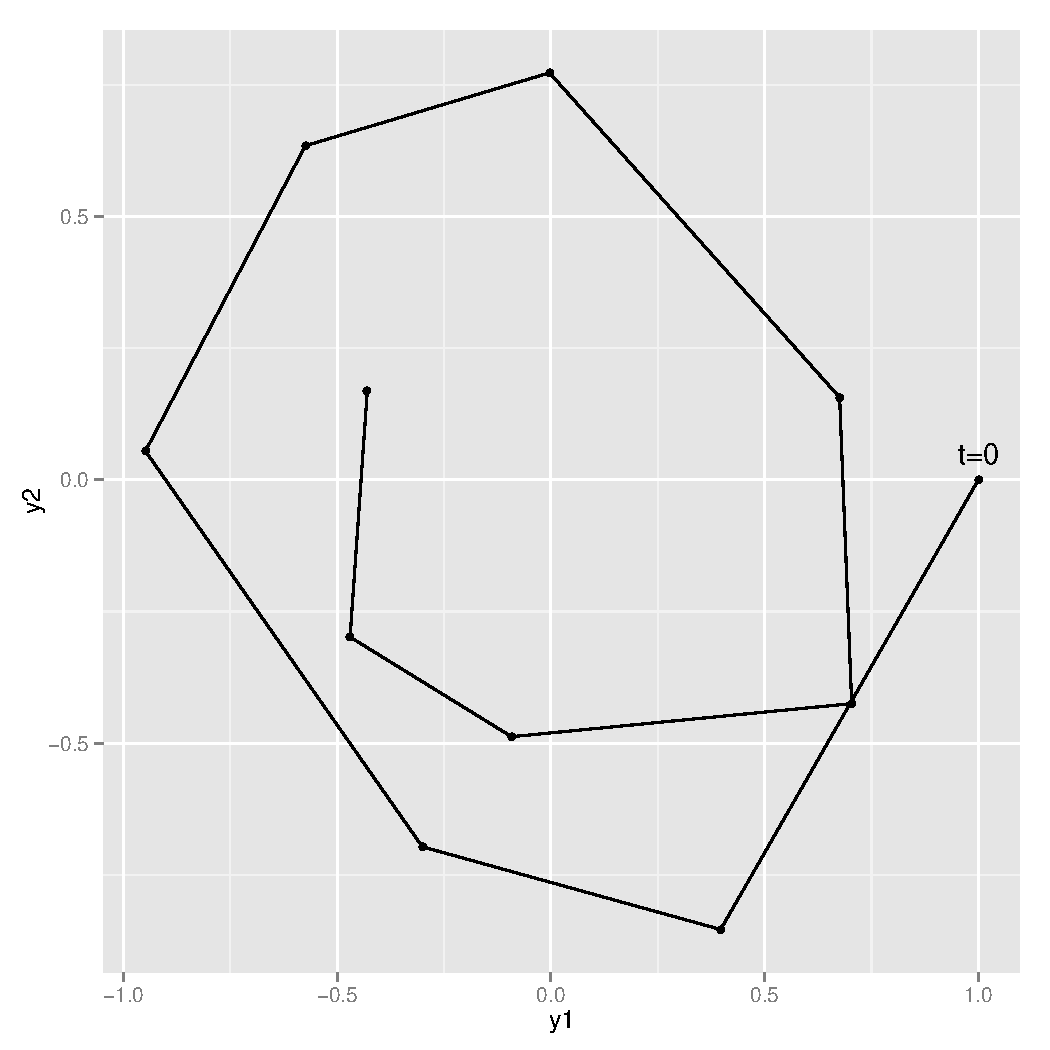
\includegraphics[height=2in]{img/sho-ode-trajectory.pdf}%
\end{center}
\vspace*{-0.25in}
\caption{\small\it Trajectory of the simple harmonic oscillator given
  parameter $\theta=0.15$ and initial condition $y(t=0) = (1,0)$ with
  additional independent\ $\distro{Normal}(0,0.1)$ measurement error
  in both dimensions.}%
\label{sho-trajectory.figure}
\end{figure}



\subsection{Simulating Noisy Measurements}

The data used to make this plot is derived from the Stan model to
simulate noisy observations given in \reffigure{sho-sim}.
%
\begin{figure}
\begin{stancode}
functions {
  real[] sho(real t,
             real[] y,
             real[] theta,
             real[] x_r,
             int[] x_i) {
    real dydt[2];
    dydt[1] = y[2];
    dydt[2] = -y[1] - theta[1] * y[2];
    return dydt;
  }
}
data {
  int<lower=1> T;
  real y0[2];
  real t0;
  real ts[T];
  real theta[1];
}
transformed data {
  real x_r[0];
  int x_i[0];
}
model {
}
generated quantities {
  real y_hat[T,2] = integrate_ode_rk45(sho, y0, t0, ts, theta, x_r, x_i);
  // add measurement error
  for (t in 1:T) {
    y_hat[t, 1] += normal_rng(0, 0.1);
    y_hat[t, 2] += normal_rng(0, 0.1);
  }
}
\end{stancode}
\vspace*{-0.2in}
\caption{\small\it Stan program to simulate noisy measurements from a
  simple harmonic oscillator.  The system of differential equations is
  coded as a function.  The system parameters \code{theta} and initial
  state \code{y0} are read in as data along with the initial time
  \code{t0} and observation times \code{ts}. The generated quantities
  block is used to solve the ODE for the specified times and then add
  random measurement error, producing observations \code{y\_hat}.
  Because the system is not stiff, the \code{rk45} solver is used.}\label{sho-sim.figure}
\end{figure}

This program illustrates the way in which the ODE solver is called in
a Stan program,
%
\begin{stancode}
y_hat = integrate_ode_rk45(sho, y0, t0, ts, theta, x_r, x_i);
\end{stancode}
%
This assigns the solutions to the system defined by function
\code{sho}, given initial state \code{y0}, initial time \code{t0},
requested solution times \code{ts}, parameters \code{theta}, real data
\code{x}, and integer data \code{x\_int}.  The call explicitly
specifies the Runge-Kutta solver (for non-stiff systems).

Here, the ODE solver is called in the generated quantities block to
provide a $10 \times 2$ array of solutions \code{y\_hat} to
which measurement error is added using the normal pseudo-random number
generating function \code{normal\_rng}.  The number of rows in the
solution array is the same as the size of \code{ts}, the requested
solution times.

\subsection{Data versus Parameters}

Unlike other functions, the integration functions for ODEs are limited
as to the origins of variables in their arguments.  In particular, the
time \code{t}, real data \code{x}, and integer data \code{x\_int} must
be expressions that only involve data or transformed data variables.
The initial state \code{y} or the parameters \code{theta} are the only
arguments which may involve parameters.


\subsection{Estimating System Parameters and Initial State}

Stan provides statistical inference for unknown initial states and/or
parameters.  The ODE solver will be used deterministically to produce
predictions, much like the linear predictor does in a generalized
linear model.  These states will then be observed with measurement error.

%
\begin{figure}
\begin{stancode}
functions {
  real[] sho(real t,
             real[] y,
             real[] theta,
             real[] x_r,
             int[] x_i) {
    real dydt[2];
    dydt[1] = y[2];
    dydt[2] = -y[1] - theta[1] * y[2];
    return dydt;
  }
}
data {
  int<lower=1> T;
  real y[T,2];
  real t0;
  real ts[T];
}
transformed data {
  real x_r[0];
  int x_i[0];
}
parameters {
  real y0[2];
  vector<lower=0>[2] sigma;
  real theta[1];
}
model {
  real y_hat[T,2];
  sigma ~ cauchy(0, 2.5);
  theta ~ std_normal();
  y0 ~ std_normal();
  y_hat = integrate_ode_rk45(sho, y0, t0, ts, theta, x_r, x_i);
  for (t in 1:T)
    y[t] ~ normal(y_hat[t], sigma);
}
\end{stancode}
\vspace*{-0.2in}
\caption{\small\it Stan program to estimate unknown initial conditions
  \code{y0} and system parameter \code{theta} for the simple harmonic
  oscillator with independent normal measurement
  error.}\label{sho-both.figure}
\end{figure}
%
A Stan program that can be used to estimate both the initial state and
parameter value for the simple harmonic oscillator given noisy
observations is given in \reffigure{sho-both}.  Compared to the
simulation model in \reffigure{sho-sim}, the model to estimate
parameters uses the \code{integrate\_ode} function in the model block
rather than the generated quantities block.  There are Cauchy priors on the
measurement error scales \code{sigma} and standard normal priors on the
components of parameter array \code{theta} and initial state parameter
array \code{y0}.  The solutions to the ODE are then assigned to an
array \code{y\_hat}, which is then used as the location in the
observation noise model as follows.
%
\begin{stancode}
y_hat = integrate_ode_rk45(sho, y0, t0, ts, theta, x_r, x_i);
for (t in 1:T)
  y[t] ~ normal(y_hat[t], sigma);
\end{stancode}
%
As with other regression-like models, it's easy to change the noise
model to be robust (e.g., Student-t distributed), to be correlated in
the state variables (e.g., with a multivariate normal distribution),
or both (e.g., with a multivariate Student-t distribution).

In this simple model with independent noise scales of 0.10, 10
observed data points for times $t = 1, ..., 10$ is sufficient to
reliably estimate the ODE parameter, initial state, and noise scales.


\section{Stiff ODEs}\label{stiff-ode.section}

A stiff system of ordinary differential equations can be roughly
characterized as systems presenting numerical difficulties for
gradient-based stepwise solvers.  Stiffness typically arises due to
varying curvature in the dimensions of the state, for instance one
component evolving orders of magnitude more slowly than another.%
%
\footnote{Not coincidentally, high curvature in the posterior of a
  general Stan model poses the same kind of problem for Euclidean
  Hamiltonian Monte Carlo (HMC) sampling.  The reason is that HMC is
  based on the leapfrog algorithm, a gradient-based, stepwise
  numerical differential equation solver specialized for Hamiltonian
  systems with separable potential and kinetic energy terms.}
%

Stan provides a specialized solver for stiff ODEs
\citep{CohenHindmarsh:1996,SerbanHindmarsh:2005}.  An ODE system is
specified exactly the same way with a function of exactly the same
signature.  The only difference is in the call to the integrator for
the solution; the \code{rk45} suffix is replaced with \code{bdf}, as in
%
\begin{stancode}
y_hat = integrate_ode_bdf(sho, y0, t0, ts, theta, x_r, x_i);
\end{stancode}
%

Using the stiff (\code{bdf}) integrator on a system that is not stiff
may be much slower than using the non-stiff (\code{rk45}) integrator;
this is because it computes additional Jacobians to guide the
integrator.  On the other hand, attempting to use the non-stiff
integrator for a stiff system will fail due to requiring a small step
size and too many steps.

\section{Control Parameters for ODE Solving}

The calls to the integrators shown above just used the default
control settings.  Both the non-stiff and stiff integrators allow
three additional arguments, all of which must be supplied if any of
them is required.
%
\begin{stancode}
y_hat = integrate_ode_bdf(sho, y0, t0, ts, theta, x_r, x_i,
                          rel_tol, abs_tol, max_steps);
\end{stancode}
%
The three control arguments are relative tolerance, absolute
tolerance, and maximum number of steps.   The default values for
relative and absolute tolerance are both \code{1e-6} ($10^{-6}$), and
the default maximum number of steps is \code{1e6} ($10^6$).

\subsection{Data only for control parameters}

The control parameters must be data variables---they can not be
parameters or expressions that depend on parameters, including local
variables in any block other than transformed data and generated
quantities.  User-defined function arguments may be qualified as only
allowing data arguments using the \code{data} qualifier.

\subsection{Tolerance}

The relative and absolute tolerance control the accuracy of the
solutions generated by the integrator.  Relative tolerances are
relative to the solution value, whereas absolute tolerances is the
maximum absolute error allowed in a solution.

Smaller tolerances produce more accurate solutions.  Smaller
tolerances also require more computation time.

\subsubsection{Sensitivity Analysis}

The tolerances should be set low enough that setting them lower does
not change the statistical properties of posterior samples generated
by the Stan program.

\subsection{Maximum Number of Steps}

The maximum number of steps can be used to stop a runaway simulation.
This can arise in MCMC when a bad jump is taken, particularly during
warmup.  With the non-stiff solver, this may result in jumping into a
stiff region of the parameter space, which would require a very small
step size and very many steps to satisfy even modest tolerances.


\chapter{Computing One Dimensional Integrals}

\noindent
Definite and indefinite one dimensional integrals can be performed in Stan via the \code{integrate\_1d} function.

As an example, the Mat\'ern covariance kernel can be written

\begin{align}
k_\nu(r) = \frac{2^{1 - \nu}}{\Gamma(\nu)} \left( \frac{\sqrt{2 \nu} r}{l} \right)^\nu K_\nu \left( \frac{\sqrt{2 \nu} r}{l} \right)
\end{align}

\noindent where K_\nu is a modified Bessel function of the second time. For general cases of $\nu$, this Bessel function can be computed
with the definite integral given in \cite{Rothwell:2008}.

\begin{align}
K_\nu(z) = \frac{\pi}{\Gamma(\nu + \frac{1}{2})} (2 z)^{-\nu} e^{-z} \int_0^1 [\beta e^{-x^\beta} (2 z + x^\beta)^{\nu - \frac{1}{2}} x^{n - 1} e^{-\frac{1}{x}} x^{-2 \nu - 1} (2 z x + 1)^{\nu - \frac{1}{2}}] dx
\end{align}

\noindent where

\begin{align}
\beta = \frac{2 n}{2 \nu + 1}
\end{align}

\noindent
$n$ is set to $8$, mimicking \ref{Rothwell:2008}. To compute this integral in Stan, the integrand must first be defined as a Stan function (see \refchapter{functions-programming} for more information on coding user-defined functions).

\begin{stancode}
real Kv_int(real x,          // Function argument
            real xc,         // Complement of function argument
                             //  on the domain (defined later)
            real[] theta,    // parameters
            real[] x_r,      // data (real)
            int[] x_i) {     // data (integer)
  real nu = theta[1];
  real beta = 16.0 / (2.0 * nu + 1.0);

  real first = beta * exp(-pow(x, beta)) * pow(2 * z + pow(x, beta), nu - 0.5) * pow(x, 7);
  real second = exp(-1.0 / x);
  if (second > 0) {
    second = second * pow(x, -2 * nu - 1) * pow(2 * z * x + 1, v - 0.5);
  }
  
  return first + second;
}
\end{stancode}
%

\noindent
This function is expected to return the value of the integrand evaluated at point \code{x}. The
argument \code{xc} is used in definite integrals to avoid loss of precision near
the limits of integration and is set to NaN when either limit is infinite
(see \refsection{integral-precision} for details on how to use this). The argument
\code{theta} is used to pass in arguments of the integral
that are a function of the parameters in our model. The arguments \code{x\_r}
and \code{x\_i} are likewise used to pass in arguments of the integral that are data.

\subsubsection{Strict Signature}
%
The function defining the integrand must have exactly the argument types and
return type of \code{normal\_density} above, though argument naming is not important.
Even if \code{x\_r} and \code{x\_i} are unused in the integrand, they must be
included in the function signature. This may require passing in zero-length arrays
for data or a zero-length vector for parameters if the integral does not involve
data or parameters.

\section{Calling the 1D Integrator}
%
Suppose that our model requires evaluating the lpdf of a left-truncated normal, but
the truncation limit is to be estimated as a parameter. Because the truncation
point is a parameter, we must include the normalization term of the truncated pdf when
computing our model's log density. Note this is just an example of how to use the
1D integrator. The more efficient way to perform the correct normalization in Stan
is described in \refchapter{truncated-data}.

Such a model might look like (including the function defined above):

%
\begin{stancode}
data {
  int N;
  real y[N];
}

transformed data {
  real x_r[0];
  int x_i[0];
}

parameters {
  real mu;
  real<lower = 0.0> sigma;
  real left_limit;
}

model {
  mu ~ normal(0, 1);
  sigma ~ normal(0, 1);
  left_limit ~ normal(0, 1);
  target += normal_lpdf(y | mu, sigma);
  target += log(integrate_1d(normal_density, left_limit, positive_infinity(), { mu, sigma }, x_r, x_i));
}
\end{stancode}
%
\subsection{Limits of integration}
The limits of integration can be finite or infinite. The infinite limits are made available via
the Stan calls \code{negative\_infinity()} and \code{positive\_infinity()}.

If both limits are either \code{negative\_infinity()} or \code{positive\_infinity()}, the integral
and its gradients are set to zero.

\subsection{Data versus Parameters}
%
The arguments for the real data \code{x\_r} and the integer data \code{x\_i}
must be expressions that only involve data or transformed data variables.
\code{theta}, on the other hand, can be a function of data, transformed data,
parameters, or transformed parameters.

The endpoints of integration can be data or parameters (and interally the
derivatives of the integral with respect to the endpoints are handled
with the Leibniz integral rule).

\section{Integrator convergence}
%
The integral is performed with the iterative 1D quadrature methods implemented in the Boost library \cite{BoostQuadrature:2017}. If the nth estimate of the integral is denoted $I_n$ and the nth estimate of the norm of the integral is denoted $|I|_n$, the iteration is terminated when

\begin{align*}
  \frac{{|I_{n + 1} - I_n|}}{{|I|_{n + 1}}} < \text{relative tolerance}
\end{align*}

\noindent
The \code{relative\_tolerance} parameter can be optionally specified as the last argument to \code{integrate\_1d} and defaults to the square root of the machine epsilon of double precision floating point numbers (that is a relative tolerance of around \code{1.5e-8}).

\subsection{Zero-crossing integrals} \label{zero-crossing.section}
Integrals on the (possibly infinite) interval $(a, b)$ that cross zero are split into two integrals, one from $(a, 0)$ and one from $(0, b)$. This is because the quadrature methods employed internally can have difficulty near zero.

In this case, each integral is separately integrated to the given \code{relative\_tolerance}.

\subsection{Avoiding precision loss near limits of integration in definite integrals} \label{integral-precision.section}

If care is not taken, the quadrature can suffer from numerical loss of precision near the endpoints of definite integrals.

For instance, in integrating the pdf of a beta distribution when the values of $\alpha$ and $\beta$ are small, most of the probability mass is lumped near zero and one.

The pdf of a beta distribution is proportional to
\begin{align*}
p(x) \propto x^{\alpha - 1}(1 - x)^{\beta - 1}
\end{align*}

\noindent
Normalizing this distribution requires computing the integral of $p(x)$ from zero to one. In Stan code, the integrand might look like:

%
\begin{stancode}
real beta(real x, real xc, real[] theta, real[] x_r, int[] x_i) {
  real alpha = theta[1];
  real beta = theta[2];

  return x^(alpha - 1.0) * (1.0 - x)^(beta - 1.0);
}
\end{stancode}
%

\noindent
The issue is that there will be numerical breakdown in the precision of \code{1.0 - x} as \code{x} gets close to one. This is because of the limited precision of double precision floating numbers. This integral will fail to converge for values of \code{alpha} and \code{beta} much less than one.

This is where \code{xc} is useful. It is defined, for definite integrals, as a high precision version of the distance from \code{x} to the nearest endpoint. To make use of this for the beta integral, the integrand can be re-coded:

%
\begin{stancode}
real beta(real x, real xc, real[] theta, real[] x_r, int[] x_i) {
  real alpha = theta[1];
  real beta = theta[2];
  real v;

  if(x > 0.5) {
    v = x^(alpha - 1.0) * xc^(beta - 1.0);
  } else {
    v = x^(alpha - 1.0) * (1.0 - x)^(beta - 1.0);
  }

  return v;
}
\end{stancode}
%

\noindent
This version of the integrand will converge for much smaller values of \code{alpha} and \code{beta} than otherwise possible.

Note, \code{xc} is only used for definite integrals. If either the left endpoint is at negative infinity or the right endpoint is at positive infinity, \code{xc} will be NaN.

For zero-crossing definite integrals (see \refsection{zero-crossing}) the integrals are broken into two pieces ($(a, 0)$ and $(0, b)$ for endpoints $a < 0$ and $b > 0$) and \code{xc} is a high precision version of the distance to the limits of each of the two integrals separately. This means \code{xc} will be the a high precision version of \code{a - x}, \code{x}, or \code{b - x}, depending on the value of x and the endpoints.


\part{Programming Techniques}\label{programming-techniques.part}


\chapter{Model Building as Software Development}

\noindent
Developing a Stan model is a software development process.  Developing
software is hard.  Very hard.  So many things can go wrong because
there are so many moving parts and combinations of parts.  

Software development practices are designed to mitigate the problems
caused by the inherent complexity of software development.
Unfortunately, many methodologies veer off into dogma, bean counting,
or both.  A couple we can recommend that provide solid, practical
advice for developers are \citep{HuntThomas:99} and
\citep{McConnell:2004}.  This section tries to summarize some of their
advice.

\section{Use Version Control}

Version control software, such as Subversion or Git, should be in
place before starting to code.%
%
\footnote{Stan started using Subversion (SVN), then switched to the
  much more feature-rich Git package.  Git does everything SVN does
  and a whole lot more.  The price is a steeper learning curve.  For
  individual or very-small-team development, SVN is just fine.}
%
It may seem like a big investment to learn version control, but it's
well worth it to be able to type a single command to revert to a
previously working version or to get the difference between the
current version and an old version.  It's even better when you need
to share work with others, even on a paper.


\section{Make it Reproducible}

Rather than entering commands on the command-line when running models
(or entering commands directly into an interactive programming
language like R or Python), try writing scripts to run the data
through the models and produce whatever posterior analysis you need.
Scripts can be written for the shell, R, or Python.  Whatever language
a script is in, it should be self contained and not depend on global
variables having been set, other data being read in, etc.  

\subsection{Scripts are Good Documentation}

It may seem like overkill if running the project is only a single line
of code, but the script provides not only a way to run the code, but
also a form of concrete documentation for what is run. 


\subsection{Randomization and Saving Seeds}

Randomness defeats reproducibility.  MCMC methods are conceptually
randomized.  Stan's samplers involve random initializations as well as
randomization during each iteration (e.g., Hamiltonian Monte Carlo
generates a random momentum in each iteration).

Computers are deterministic.  There is no real randomness, just
pseudo-random number generators.  These operate by generating a
sequence of random numbers based on a ``seed.''  Stan (and other
languages like R) can use time-based methods to generate a seed based
on the time and date, or seeds can be provided to Stan (or R) in the
form of long integers.  Stan writes out the seed used to generate the
data as well as the version number of the Stan software so that
results can be reproduced at a later date.%
%
\footnote{This also requires fixing compilers and hardware, because
  floating-point arithmetic does not have an absolutely fixed behavior
  across platforms or compilers, just operating parameters.}



\section{Make it Readable}

Treating programs and scripts like other forms of writing for an
audience provides an important perspective on how the code will be
used.  Not only might others want to read a program or model, the
developer will want to read it later.  One of the motivations of
Stan's design was to make models self-documenting in terms of variable
usage (e.g., data versus parameter), types (e.g., covariance matrix
vs. unconstrained matrix) and sizes.  

A large part of readability is consistency.  Particularly in naming
and layout.  Not only of programs themselves, but the directories and
files in which they're stored.

Readability of code is not just about comments (see
Section~\refsection{comments-programming} for commenting
recommendations and syntax in Stan).

It is surprising how often the solution to a debugging or design
problem occurs when trying to explain enough about the problem to
someone else to get help.  This can be on a mailing list, but it works
best person-to-person.  Finding the solution to your own problem when
explaining it to someone else happens so frquently in software
development that the listener is called a ``rubber ducky,'' because
they only have to nod along.%
%
\footnote{Research has shown an actual rubber ducky won't work.  For
  some reason, the rubber ducky must actually be capable of
  understanding the explanation.}


\section{Explore the Data}

Although this should go without saying, don't just fit data blindly.
Look at the data you actually have to understand its properties.  If
you're doing a logistic regression, is it separable?  If you're
building a multilevel model, do the basic outcomes vary by level?  If
you're fitting a linear regression, see whether such a model makes
sense by scatterplotting $x$ vs. $y$.

\section{Design Top-Down, Code Bottom-Up}

Software projects are almost always designed top-down from one or more
intended use cases.  Good software coding, on the other hand, is
typically done bottom-up.  

The motivation for top-down design is obvious.  The motivation for
bottom-up development is that it is much easier to develop software
using components that have been thoroughly tested.  Although Stan has
no built-in support for either modularity or testing, many of the same
principles apply.  

The way the developers of Stan themselves build models is to start as
simply as possibly, then build up. This is true even if we have a
complicated model in mind as the end goal, and even if we have a very
good idea of the model we eventually want to fit.  Rather than
building a hierarchical model with multiple interactions, covariance
priors, or other complicated structure, start simple.  Build just a
simple regression with fixed (and fairly tight) priors.  Then add
interactions or additional levels.  One at a time.  Make sure that
these do the right thing.  Then expand.

\section{Fit Simulated Data}

One of the best ways to make sure your model is doing the right thing
computationally is to generate simulated (i.e., ``fake'') data with
known parameter values, then see if the model can recover these
parameters from the data.  If not, there is very little hope that it
will do the right thing with data from the wild.  

There are fancier ways to do this, where you can do things like run
$\chi^2$ tests on marginal statistics or follow the paradigm
introduced in \citep{CookGelmanRubin:2006}, which involves interval
tests.  

\section{Debug by Print}

Although Stan does not have a stepwise debugger or any unit testing
framework in place, it does support the time-honored tradition of
debug-by-printf.
%
\footnote{The ``f'' is not a typo --- it's a historical artifact of
  the name of the \code{printf} function used for formatted printing
  in C.} 

Stan supports print statements with one or more string or expression
arguments.  Because Stan is an imperative language, variables can have
different values at different points in the execution of a program.
Print statements can be invaluable for debugging, especially for a
language like Stan with no stepwise debugger.

For instance, to print the value of variables \code{y} and
\code{z}, use the following statement.
%
\begin{quote}
\begin{Verbatim}[fontsize=\small]
print("y=", y, " z=", z);
\end{Verbatim}
\end{quote}
%
This print statement prints the string ``y='' followed by the value of
\code{y}, followed by the string `` z=''
(with the leading space), followed by the value of the variable
\code{z}.

Each print statement is followed by a new line.  The specific ASCII
character(s) generated to create a new line are platform specific.

Arbitrary expressions can be used.  For example, the statement
\begin{quote}
\begin{Verbatim}[fontsize=\small]
print("1+1=", 1+1);
\end{Verbatim}
\end{quote}
%
will print ``1 + 1 = 2'' followed by a new line.

Print statements may be used anywhere other statements may be used,
but their behavior in terms of frequency depends on how often the
block they are in is evaluated.  See \refsection{print-statements} for
more information on the syntax and evaluation of print statements.



\section{Comments}\label{comments-programming.section}

\subsection{Code Never Lies}

The machine does what the code says, not what the documentation says.
Docuementation, on the other hand, might not match the code.  Code
documentation easily rots as the code evolves if the documentation is
not well maintained.  

Thus it is always preferable to write readable code as opposed to
documenting unreadable code.  Every time you write a piece of
documentation, ask yourself if there's a way to write the code in such
a way as to make the documentation unnecessary.


\subsection{Comment Styles in Stan}

Stan supports \Cpp-style comments; see \refsection{comments} for full
details.  The recommended style is to use line-based comments for
short comments on the code or to comment out one or more
lines of code.  Bracketed comments are then reserved for long
documentation comments.  The reason for this convention is that
bracketed comments cannot be wrapped inside of bracketed comments.

\subsection{What Not to Comment}

When commenting code, it is usually safe to assume that you are 
writing the comments for other programmers who understand the basics 
of the programming language in use.  In other words, don't comment the
obvious.  For instance, there is no need to have comments
such as the following, which add nothing to the code.
%
\begin{quote}
\begin{Verbatim}[fontsize=\small]
y ~ normal(0,1);  // y has a unit normal distribution
\end{Verbatim}
\end{quote}
%
A Jacobian adjustment for a hand-coded transform might be worth
commenting, as in the following example.
%
\begin{quote}
\begin{Verbatim}[fontsize=\small]
exp(y) ~ normal(0,1);
// adjust for change of vars: y = log | d/dy exp(y) |
increment_log_prob(y);
\end{Verbatim}
\end{quote}
%
It's an art form to empathize with a future code reader and decide
what they will or won't know (or remember) about statistics and Stan.

\subsection{What to Comment}

It can help to document variable declarations if variables are given
generic names like \code{N}, \code{mu}, and \code{sigma}.  For
example, some data variable declarations in an item-response model
might be usefully commented as follows.
%
\begin{quote}
\begin{Verbatim}[fontsize=\small]
int<lower=1> N;   // number of observations
int<lower=1> I;   // number of students
int<lower=1> J;   // number of test questions
\end{Verbatim}
\end{quote}
%
The alternative is to use longer names that do not require comments.
%
\begin{quote}
\begin{Verbatim}[fontsize=\small]
int<lower=1> n_obs;
int<lower=1> n_students;
int<lower=1> n_questions;
\end{Verbatim}
\end{quote}
%
Both styles are reasonable and which one to adopt is mostly a matter of
taste (mostly because sometimes models come with their own naming
conventions which should be followed so as not to confuse readers of
the code familiar with the statistical conventions).

Some code authors like big blocks of comments at the top explaining
the purpose of the model, who wrote it, copyright and licensing
information, and so on.  The following bracketed comment is an
example of a conventional style for large comment blocks.
%
\begin{quote}
\begin{Verbatim}[fontsize=\small]
/*
 * Item-Response Theory PL3 Model
 * -----------------------------------------------------
 * Copyright: Joe Schmoe  <joe@schmoe.com>
 * Date:  19 September 2012
 * License: GPLv3
 */

data {
  ...
\end{Verbatim}
\end{quote}
%
The use of leading asterisks helps readers understand the scope of the
comment.  The problem with including dates or other volatile
information in comments is that they can easily get out of synch with
the reality of the code.  A misleading comment or one that is wrong is
worse than no comment at all!


\chapter{Containers: Arrays, Vectors, and Matrices}

\noindent
Stan provides three types of container objects: arrays, vectors, and
matrices.  The three types are not interchangeable.  Vectors, matrices,
and arrays are not assignable to one another, even if their dimensions
are identical.  A $3 \times 4$ matrix is a different kind of object in
Stan than a $3 \times 4$ array. 

\section{Vectors and Matrices}

Vectors and matrices are more limited kinds of data structures than
arrays.  Vectors are intrinsically one-dimensional collections of
reals, whereas matrices are intrinsically two dimensional. 

The intention of using matrix types is to call out their usage in the
code.  There are three situations in Stan where {\it only} vectors and
matrices may be used,
%
\begin{itemize}
\item matrix arithmetic operations (e.g., matrix multiplication)
\item linear algebra functions (e.g., eigenvalues and determinants),
  and
\item multivariate function parameters and outcomes (e.g.,
  multivariate normal distribution arguments).
\end{itemize}
%

Vectors and matrices cannot be typed to return integer values.  They
are restricted to \code{real} values.%
%
\footnote{This may change if Stan is called upon to do complicated
  integer matrix operations or boolean matrix operations.  Integers
  are not appropriate inputs for linear algebra functions.}

\section{Arrays}

Arrays, on the other hand, are intrinsically one-dimensional
collections of other kinds of objects.  The values in an array can be
any type, so that arrays may contain values that are simple reals or
integers, vectors, matrices, or other arrays.  Arrays are the only way
to store sequences of integers, and some functions in Stan, such as
discrete distributions, require integer arguments. 


A two-dimensional array is just an array of arrays, both conceptually
and in terms of current implementation.  When an index is supplied to
an array, it returns the value at that index.  When more than one
index is supplied, this idexing operation is chained.  For example, if
\code{a} is a two-dimensional array, then \code{a[m,n]} is just
a convenient shorthand for \code{a[m][n]}.


\section{Efficiency Considerations}

One of the motivations for Stan's underlying design is efficiency.

The underlying matrix and linear algebra operations are implemented in
terms of data types from the Eigen \Cpp library.  By having vectors
and matrices as basic types, no conversion is necessary when invoking
matrix operations or calling linear algebra functions.  

Arrays, on the other hand, are implemented as instances of the \Cpp \ 
\code{std::vector} class (not to be confused with Eigen's
\code{Eigen::Vector} class or Stan vectors).  By implementing arrays
this way, indexing is very efficient because values can be returned by
reference rather than copied by value.

\subsection{Matrices vs.\ Two-Dimensional Arrays}

In Stan models, there are a few minor efficiency considerations in
deciding between a two-dimensional array and a matrix, which may seem
interchangeable at first glance.  

First, matrices use a bit less memory than two-dimensional arrays.
This is because they don't store a sequence of arrays, but just the
data and the two dimensions.  

Second, matrices store their data in row-major order.  Furthermore,
all of the data in a matrix is guaranteed to be contiguous in memory.
This is an important consideration for optimized code because bringing
in data from memory to cache is much more expensive than performing
arithmetic operations with contemporary CPUs.  Arrays, on the other
hand, only guarantee that the values of primitive types are contiguous
in memory; otherwise, they hold copies of their values (which are
returned by reference wherever possible).

Third, both data structures are best traversed in the order in which
they are stored.  This also helps with memory locality.  This is
column-major for matrices, so the following order is appropriate.
%
\begin{quote}
\begin{Verbatim}
matrix[M,N] a;
...
for (n in 1:N)
  for (m in 1:M)
    ... do something with a[m,n] ...
\end{Verbatim}
\end{quote}
%
Arrays, on the other hand, should be traversed in row-major order.
%
\begin{quote}
\begin{Verbatim}
real a[M,N];
...
for (m in 1:M)
  for (n in 1:N)
    ... do something with a[m,n] ...
\end{Verbatim}
\end{quote}
%
The first use of \code{a[m,n]} should bring \code{a[m]} into memory.
Overall, traversing matrices is more efficient than traversing arrays.

If \code{a} is a matrix, the notation \code{a[m]} picks out row
\code{m} of that matrix.  This is a rather inefficient operation for
matrices.  If indexing of vectors is needed, it is much better to
declare an array of vectors.  That is, this
%
\begin{quote}
\begin{Verbatim}
row_vector[N] b[M];
...
for (m in 1:M)
   ... do something with row vector b[m] ...
\end{Verbatim}
\end{quote}
%
is much more efficient than the pure matrix version
%
\begin{quote}
\begin{Verbatim}
matrix b[M,N];
...
for (m in 1:M)
   ... do something with row vector b[m] ...
\end{Verbatim}
\end{quote}
%
Similarly, indexing an array of column vectors is more efficient than
using the \code{col} function to pick out a column of a matrix.

In contrast, whatever can be done as pure matrix algebra will be the
fastest.  So if I want to create a row of predictor-coefficient
dot-products, it's more efficient to do this
%
\begin{quote}
\begin{Verbatim}
matrix[N,K] x;    // predictors (aka covariates)
...
vector[K] beta;   // coeffs
...
vector[N] y_hat;  // linear prediction
...
y_hat <- x * beta;
\end{Verbatim}
\end{quote}
%
than it is to do this
%
\begin{quote}
\begin{Verbatim}
row_vector[K] x[N];    // predictors (aka covariates)
...
vector[K] beta;   // coeffs
...
vector[N] y_hat;  // linear prediction
...
for (n in 1:N)
  y_hat[n] <- x[n] * beta;
\end{Verbatim}
\end{quote}

\subsection{(Row) Vectors vs. One-Dimensional Arrays}

For use purely as a container, there is really nothing to decide among
vectors, row vectors and one-dimensional arrays.  The
\code{Eigen::Vector} template specialization and the
\code{std::vector} template class are implemented very similarly as
containers of \code{double} values (the type \code{real} in Stan).
Only arrays in Stan are allowed to store integer values.




\chapter{Missing Data \& Partially Known Parameters}

\noindent
\BUGS and \R support mixed arrays of known and missing data.  In
\BUGS, known and unknown values may be mixed as long as every unknown
variable appears on the left-hand side of either an assignment or
sampling statement.  

\section{Missing Data}


\Stan treats variables declared in the \code{data} and
\code{transformed data} blocks as known and the variables in the
\code{parameters} block as unknown.

The next section shows how to create a mixed array of known and
unknown values as in \BUGS.  The recommended approach to missing data
in \Stan is slightly different than in \BUGS.  An example involving
missing normal observations%
%
\footnote{A more meaningful estimation example would involve a
  regression of the observed and missing observations using predictors
  that were known for each and specified in the \code{data} block.}
%
could be coded as follows.
%
\begin{quote}
\begin{Verbatim}[fontsize=\small]
data {
  int<lower=0> N_obs;
  int<lower=0> N_miss;
  real y_obs[N_obs];
}
parameters {
  real mu;
  real<lower=0> sigma;
  real y_miss[N_miss];
}
model {
  for (n in 1:N_obs)
    y_obs[n] ~ normal(mu,sigma);
  for (n in 1:N_miss)
    y_miss[n] ~ normal(mu,sigma);
}
\end{Verbatim}
\end{quote}
%
The number of observed and missing data points are coded as data with
non-negative integer variables \code{N\_obs} and \code{N\_miss}.  The
observed data is provided as an array data variable \code{y\_obs}.
The missing data is coded as an array parameter, \code{y\_miss}.  The
ordinary parameters being estimated, the location \code{mu} and scale
\code{sigma}, are also coded as parameters.  A better way to write the
model would be to vectorize, so the body would be
%
\begin{quote}
\begin{Verbatim}[fontsize=\small]
   y_obs ~ normal(mu,sigma);
   y_miss ~ normal(mu,sigma);
\end{Verbatim}
\end{quote}

The model contains one loop over the observed data and one over the
missing data.  This slight redundancy in specification leads to much
more efficient sampling for missing data problems in \Stan than the
more general technique described in the next section.


\section{Partially Known Parameters}\label{partially-known-parameters.section}

In some situations, such as when a multivariate probability function
has partially observed outcomes or parameters, it will be necessary to
create a vector mixing known (data) and unknown (parameter) values.
This can be done in \Stan by creating a vector or array in the
\code{transformed parameters} block and assigning to it.

The following example involves a bivariate covariance matrix in which the
variances are known, but the covariance is not.
%
\begin{quote}
\begin{Verbatim}[fontsize=\small]
data {
  int<lower=0> N;
  vector[2] y[N];
  real<lower=0> var1;     real<lower=0> var2;
}
transformed data {
  real<upper=0> min_cov;   
  real<lower=0> max_cov;  
  max_cov <- sqrt(var1 * var2);  
  min_cov <- -max_cov;
}
parameters {
  vector[2] mu;
  real<lower=min_cov,upper=max_cov> cov;
}
transformed parameters {
  matrix[2,2] sigma;
  sigma[1,1] <- var1;     sigma[1,2] <- cov;
  sigma[2,1] <- cov;      sigma[2,2] <- var2;
}  
model {
 for (n in 1:N)
   y[n] ~ multi_normal(mu,sigma);
}
\end{Verbatim}
\end{quote}
%
The variances are defined as data in variables \code{var1} and
\code{var2}, whereas the covariance is defined as a parameter in
variable \code{cov}.  The $2 \times 2$ covariance matrix
\code{sigma} is defined as a transformed parameter, with the variances
assigned to the two diagonal elements and the covariance to the two
off-diagonal elements.

The constraint on the covariance declaration ensures that the
resulting covariance matrix \code{sigma} is positive definite.  The
bound, plus or minus the square root of the product of the variances,
is defined as transformed data so that it is only calculated once.

\section{Efficiency Note}

The missing-data example in the first section could be programmed with
a mixed data and parameter array following the approach of the
partially known parameter example in the second section.  The behavior
will be correct, but the computation is wasteful.  Each parameter, be
it declared in the \code{parameters} or \code{transformed parameters}
block, uses an algorithmic differentiation variable which is more
expensive in terms of memory and gradient-calculation time than a
simple data variable.  Furthermore, the copy takes up extra space and
extra time.


\chapter{Truncated or Censored Data}

\noindent
Data in which measurements have been truncated or censored can be
coded in Stan following their respective probability models.

\section{Truncated Distributions}

Truncation in Stan is restricted to univariate distributions for which
the corresponding log cumulative distribution function (cdf) and log
completmentary cumulative distribution (ccdf) functions are
available.  See \refsection{truncated-distributions} for more
information on truncated distributions, cdfs, and ccdfs.

\section{Truncated Data}

Truncated data is data for which measurements are only reported if
they fall above a lower bound, below an upper bound, or between a
lower and upper bound.  

Truncated data may be modeled in \Stan using truncated distributions.
For example, suppose the truncated data is $y_n$ with an upper
truncation point of $U = 300$ so that $y_n < 300$.  In \Stan, this
data can be modeled as following a truncated normal distribution for
the observations as follows. 
%
\begin{quote}
\begin{Verbatim}[fontsize=\small]
data {
  int<lower=0> N;
  real U;
  real<upper=U> y[N];
} 
parameters {
  real mu;
  real<lower=0> sigma;
} 
model {
  for (n in 1:N)
    y[n] ~ normal(mu,sigma) T[,U];
}
\end{Verbatim}
\end{quote}
% 
The model declares an upper bound \code{U} as data and constrains
the data for \code{y} to respect the constraint;  this will be checked
when the data is loaded into the model before sampling begins.

This model implicitly uses an improper flat prior on the scale and
location parameters; these could be given priors in the model using
sampling statements.

\subsection{Constraints and Out-of-Bounds Returns}\label{truncation-constraints.section}

If the sampled variate in a truncated distribution lies outside of
the truncation range, the probability is zero, so the log probability
will evaluate to $-\infty$.  For instance, if variate \code{y} is
sampled with the statement.
%
\begin{quote}
\begin{Verbatim}[fontsize=\small]
for (n in 1:N) 
  y[n] ~ normal(mu,sigma) T[L,U];
\end{Verbatim}
\end{quote}
%
then if the value of \code{y[n]} is less than the value of \code{L}
or greater than the value of \code{U}, the sampling statement produces
a zero-probability estimate.

To avoid variables straying outside of truncation bounds, appropriate
constraints are required.  For example, if \code{y} is a parameter in
the above model, the declaration should constrain it to fall between
the values of \code{L} and \code{U}.
%
\begin{quote}
\begin{Verbatim}[fontsize=\small]
parameters {
  real<lower=L,upper=U> y[N];
  ...
\end{Verbatim}
\end{quote}

If in the above model, \code{L} or \code{U} is a parameter and
\code{y} is data, then \code{L} and \code{U} must be appropriately
constrained so that all data is in range and the value of \code{L} is
less than that of \code{U} (if they are equal, the parameter range
collapses to a single point and the Hamiltonian dynamics used by 
the sampler break down).  The following declarations ensure the bounds
are well behaved.
%
\begin{quote}
\begin{Verbatim}[fontsize=\small]
parameters {
  real<upper=min(y)> L; // L < y[n]
  real<lower=fmax(L,max(y))> U; // L < U; y[n] < U
\end{Verbatim}
\end{quote}
%
Note that for pairs of real numbers, the function \code{fmax} is used
rather than \code{max}.







\subsection{Unknown Truncation Points}

If the truncation points are unknown, they may be estimated as
parameters.  This can be done with a slight rearrangement of the
variable declarations from the model in the previous section with
known truncation points.
%
\begin{quote}
\begin{Verbatim}[fontsize=\small]
data {
  int<lower=1> N;
  real y[N];
}
parameters {
  real<upper = min(y)> L; 
  real<lower = max(y)> U;
  real mu;
  real<lower=0> sigma;
}
model {
  L ~ ...;  
  U ~ ...;
  for (n in 1:N)
    y[n] ~ normal(mu,sigma) T[L,U];
}
\end{Verbatim}
\end{quote}
%
Here there is a lower truncation point \code{L} which is declared to
be less than or equal to the minimum value of \code{y}.  The upper
truncation point \code{U} is declared to be larger than the maximum
value of \code{y}.  This declaration, although dependent on the data,
only enforces the constraint that the data fall within the truncation
bounds.  With \code{N} declared as type \code{int<lower=1>}, there must be
at least one data point.  The constraint that \code{L} is less than
\code{U} is enforced indirectly, based on the non-empty data.

The ellipses where the priors for the bounds \code{L} and \code{U}
should go should be filled in with a an informative prior in
order for this model to not concentrate \code{L} strongly around 
\code{min(y)} and \code{U} strongly around \code{max(y)}.


\section{Censored Data}

Censoring hides values from points that are too large, too small, or
both.  Unlike with truncated data, the number of data points that were
censored is known.  The textbook example is the household scale which
does not report values above 300 pounds.  

\subsection{Estimating Censored Values}

One way to model censored data is to treat the censored data as
missing data that is constrained to fall in the censored range of
values.  Because \Stan does not allow unknown values in its arrays or
matrices, the censored values must be represented explicitly.
%
\begin{quote}
\begin{Verbatim}[fontsize=\small]
data {
  int<lower=0> N_obs;
  int<lower=0> N_cens;
  real<lower=0> y_obs[N_obs];
  real<lower=max(y_obs)> U;
}
parameters {
  real<lower=U> y_cens[N_cens];
  real mu;
  real<lower=0> sigma;
}
model {
  for (n in 1:N_obs)
    y_obs[n] ~ normal(mu,sigma);
  for (n in 1:N_cens)
    y_cens[n] ~ normal(mu,sigma);
}
\end{Verbatim}
\end{quote}
%
Because the censored data array \code{y\_cens} is declared to be a parameter, it
will be sampled along with the location and scale parameters \code{mu}
and \code{sigma}.  Because the censored data array \code{y\_cens} is
declared to have values of type \code{real<lower=U>}, all imputed values
for censored data will be greater than \code{U}.  The imputed censored
data affects the location and scale parameters through the last
sampling statement in the model.  

\subsection{Integrating out Censored Values}

Although it is wrong to ignore the censored values in estimating
location and scale, it is not necessary to impute values.  Instead,
the values can be integrated out.  Each censored data point has a
probability of
%
\[
\mbox{Pr}[y > U] 
= \int_U^{\infty} \distro{Normal}(y|\mu,\sigma) \, dy
= 1 - \Phi\left(\frac{y - \mu}{\sigma}\right),
\]
%
where $\Phi()$ is the unit normal cumulative distribution function.
With $M$ censored observations, the total probability on the log scale
is
\[
\log \prod_{m=1}^M \mbox{Pr}[y_m > U]
= \log \left( 1 - \Phi\left(\frac{y - \mu}{\sigma}\right)\right)^{M}
= M \, \log \left( 1 - \Phi\left(\frac{y - \mu}{\sigma}\right)\right)
\]
% 
Although \Stan implements $\Phi$ with the function $\code{Phi}$, \Stan
also provides the cumulative distribution function \code{normal\_cdf},
defined by
\[
\code{normal\_cdf}(y,\mu,\sigma) = \Phi \left( \frac{y - \mu}{\sigma} \right).
\]
%
The following model assumes
that the censoring point is known, so it is declared as data.
%
\begin{quote}
\begin{Verbatim}[fontsize=\small]
data {
  int<lower=0> N_obs;
  int<lower=0> N_cens;
  real<lower=0> y_obs[N_obs];
  real<lower=max(y_obs)> U;
}
parameters {
  real mu;
  real<lower=0> sigma;
}
model {
  for (n in 1:N_obs)
    y_obs[n] ~ normal(mu,sigma); 
  increment_log_prob(N_cens * log1m(normal_cdf(U,mu,sigma)));
}
\end{Verbatim}
\end{quote}
%
For the observed values in \Verb|y_obs|, the normal sampling model is
used without truncation.  The log probability is directly incremented
using the calculated log cumulative normal probability of the censored
data items.  The built-in function \code{log1m} is used, which maps
$x$ to $\log (1 - x)$ in an arithmetically stable way.

To deal with situations where the censoring point variable \code{U} is
unknown, the declaration of \code{U} should be moved from the data
block to the parameters block.



\chapter{Mixture Modeling}\label{mixture-modeling.chapter}

\noindent
Mixture models of an outcome assume that the outcome is drawn from one
of several distributions, the identity of which is controlled by a
categorical mixing distribution. Mixture models typically have
multimodal densities with modes near the modes of the mixture
components.  Mixture models may be parameterized in several ways,
as described in the following sections.


\section{Latent Discrete Parameterization}

One way to parameterize a mixture model is with a latent categorical
variable indicating which mixture component was responsible for the
outcome. For example, consider $K$ normal distributions with locations
$\mu_k \in \reals$ and scales $\sigma_k \in (0,\infty)$.  Now consider
mixing them in proportion $\theta$, where $\theta_k \geq 0$ and
$\sum_{k=1}^K \theta_k = 1$ (i.e., $\theta$ lies in the unit $K$-simplex).
For each outcome $y_n$ there is a latent variable $z_n$ in
$\setlist{1,\ldots,K}$ with a categorical distribution parameterized
by $\theta$,
%
\[
z_n \sim \distro{Categorical}(\theta).
\]
%
The variable $y_n$ is distributed according to the parameters
of the mixture component $z_n$, 
\[
y_n \sim \distro{Normal}(\mu_{z[n]},\sigma_{z[n]}).
\]
%
This model is not directly supported by \Stan because it involves
discrete parameters $z_n$, but \Stan can sample $\mu$ and $\sigma$ 
by summing out the $z$ parameter as described in the next section.


\section{Summing out the Responsibility Parameter}

To implement the normal mixture model outlined in the previous
section in \Stan, the discrete parameters can be summed out of the
model. If $Y$ is a mixture of $K$ normal distributions with 
locations $\mu_k$ and scales $\sigma_k$ with mixing proportions
$\theta$ in the unit $K$-simplex, then 
\[
p_Y(y) = \sum_{k=1}^K \theta_k \, \distro{Normal}(\mu_k,\sigma_k).
\]

For example, the mixture of $\code{Normal}(-1,2)$ and
$\code{Normal}(3,1)$ with mixing proportion $\theta =
(0.3,0.7)^{\top}$ can be implemented in \Stan as follows.
%
\begin{quote}
\begin{Verbatim}[fontsize=\small]
parameters {
  real y;
}
model {
  increment_log_prob(log_sum_exp(log(0.3) 
                                   + normal_log(y,-1,2),
                                 log(0.7) 
                                   + normal_log(y,3,1));
}
\end{Verbatim}
\end{quote}
%
The log probability term is derived by taking
\begin{eqnarray*}
\log p_Y(y) & = & \log \, \left( 0.3 \times \distro{Normal}(y|-1,2) \, + \,
  0.7 \times
  \distro{Normal}(y|3,1) \, \right)
\\[2pt]
& = & \log(\! \begin{array}[t]{l}
                 \exp(\log(0.3 \times \distro{Normal}(y|-1,2))) \\
                 + \exp(\log(0.7 \times \distro{Normal}(y|3,1))) \ )
              \end{array}
% \\[4pt]
% & = & \log( \! \begin{array}[t]{l}\exp(\log(0.3) + \log \distro{Normal}(y|-1,2))
%             \\
%            + \exp(\log(0.7) + \log \distro{Normal}(y|3,1)) \ )
%             \end{array}
\\[2pt]
& = & \mbox{log\_sum\_exp}(\! \begin{array}[t]{l}
                         \log(0.3) + \log \distro{Normal}(y|-1,2),
                         \\                  
                         \log(0.7) + \log \distro{Normal}(y|3,1) \ ).
                       \end{array}
\end{eqnarray*}

Given the scheme for representing mixtures, it may be moved to an
estimation setting, where the locations, scales, and mixture
components are unknown.  Further generalizing to a number of mixture
components specified as data yields the following model.
%
\begin{quote}
\begin{Verbatim}[fontsize=\small]
data {
  int<lower=1> K;          // number of mixture components
  int<lower=1> N;          // number of data points
  real y[N];               // observations
}
parameters {
  simplex[K] theta;        // mixing proportions
  real mu[K];              // locations of mixture components
  real<lower=0,upper=10> sigma[K];  // scales of mixture components
}
model {
  real ps[K];              // temp for log component densities
  for (k in 1:K) {
    mu[k] ~ normal(0,10);
  }
  for (n in 1:N) {
    for (k in 1:K) {
      ps[k] <- log(theta[k]) 
               + normal_log(y[n],mu[k],sigma[k]);
    }
    increment_log_prob(log_sum_exp(ps));
  }
}
\end{Verbatim}
\end{quote}
%
The model involves \code{K} mixture components and \code{N} data
points. The mixing proportion parameter \code{theta} is declared to be
a unit $K$-simplex, whereas the component location parameter \code{mu}
and scale parameter \code{sigma} are both defined to be arrays of size
\code{K}. The values in the scale array \code{sigma} are constrained
to be non-negative, and have an upper bound of 10. Since no prior is
explicitly defined for the \code{sigma} parameters, their implicit
prior distributions are uniform over their ranges. The model declares
a local array variable \code{ps} to be size \code{K} and uses it to
accumulate the contributions from the mixture components.

The locations and scales are drawn from simple priors for the sake of
this example, but could be anything supported by \Stan.  The mixture
components  could even be modeled hierarchically.

The main action is in the loop over data points \code{n}.  For each
such point, the log of $\theta_k \times
\distro{Normal}(y_n|\mu_k,\sigma_k)$ is calculated and added to the
array \code{ps}.  Then the log probability is incremented with the log
sum of exponentials of those values.





\chapter{Regression Models}

\noindent
\Stan supports regression models from simple linear regressions to
multilevel generalized linear models.  Coding regression models in
\Stan is very much like coding them in \BUGS.

\section{Linear Regression}

The simplest linear regression model is the following, with a single
predictor and a slope and intercept coefficient, and normally
distributed noise.  This model can be written using standard
regression notation as
%
\[
Y_n = \alpha + \beta x_n + \epsilon_n
\ \ \ \mbox{where} \ \ \ 
\epsilon_n \sim \distro{Normal}(0,\sigma).
\]
This is equivalent to the following sampling involving the
residual,
\[
Y_n - (\alpha + \beta X_n) \sim \distro{Normal}(0,\sigma),
\]
and reducing still further, to
\[
Y_n \sim \distro{Normal}(\alpha + \beta X_n, \, \sigma).
\]
%
This latter form of the model is coded in \Stan as follows.
%
\begin{quote}
\begin{Verbatim}[fontsize=\small]
data {
  int<lower=0> N;
  vector[N] x;
  vector[N] y;
}
parameters {
  real alpha;
  real beta;
  real<lower=0> sigma;
}
model {
  for (n in 1:N)
    y[n] ~ normal(alpha + beta * x[n], sigma);
}
\end{Verbatim}
\end{quote}
%
There are \code{N} observations, each with predictor \code{x[n]} and
outcome \code{y[n]}.  The intercept and slope parameters are
\code{alpha} and \code{beta}.  The model assumes a normally
distributed noise term with scale \code{sigma}.  This model has
improper priors for the two regression coefficients.

\section{Coefficient and Noise Priors}

There are several ways in which this model can be generalized.  
For example, weak priors can be assigned to the coefficients as follows.
%
\begin{quote}
\begin{Verbatim}[fontsize=\small]
alpha ~ normal(0,100);
beta ~ normal(0,100);
\end{Verbatim}
\end{quote}
%
And an upper bound to \code{sigma} can be given in order to implicitly
give it a uniform prior.
\begin{quote}
\begin{verbatim}
real<lower=0,upper=100> sigma;
\end{verbatim}
\end{quote}

%
More informative priors based the (half) Cauchy distribution are coded
as follows.
%
\begin{quote}
\begin{Verbatim}[fontsize=\small]
alpha ~ cauchy(0,2.5);
beta ~ cauchy(0,2.5);
sigma ~ cauchy(0,2.5);
\end{Verbatim}
\end{quote}
%
The regression coefficients \code{alpha} and \code{beta} are
unconstrained, but \code{sigma} must be positive and properly
requires the half-Cauchy distribution.  Although Stan supports
truncated distributions with half distributions being a special case,
it is not necessary here because the full distribution is proportional
when the parameters are constant.%
%
\footnote{Stan does not (yet) support truncated Cauchy distributions.
  The distributions which may be truncated are listed for discrete
  distributions in \refpart{discrete-prob-functions} and for
  continuous distributions in \refpart{continuous-prob-functions}.
  Available truncated distributions may be found in the index by
  looking for suffix \code{\_cdf}.}

\section{Robust Noise Models}

The standard approach to linear regression is to model the noise
term $\epsilon$ as having a normal distribution.  From \Stan's
perspective, there is nothing special about normally distributed
noise.  For instance, robust regression can be accommodated by giving
the noise term a Student-$t$ distribution.  To code this in \Stan, the
sampling distribution is changed to the following.
%
\begin{quote}
\begin{Verbatim}[fontsize=\small]
data {
  ...
  real<lower=0> nu;
}
...
model {
  for (n in 1:N)
    y[n] ~ student_t(nu, alpha + beta * x[n], sigma);
}
\end{Verbatim}
\end{quote}
%
The degrees of freedom constant \code{nu} is specified as data.

\section{Logistic and Probit Regression}\label{logistic-probit-regression.section}

For binary outcomes, either of the closely related logistic or probit
regression models may be used.  These generalized linear models vary
only in the link function they use to map linear predictions in
$(-\infty,\infty)$ to probability values in $(0,1)$.  Their respective
link functions, the logistic function and the unit normal cumulative distribution
function, are both sigmoid functions (i.e., they are both {\it S}-shaped).

A logistic regression model with one predictor and an intercept is coded as
follows.
%
\begin{quote}
\begin{Verbatim}[fontsize=\small]
data {
  int<lower=0> N;
  real x[N];
  int<lower=0,upper=1> y[N];
}
parameters {
  real alpha;
  real beta;
}
model {
  for (n in 1:N)
    y[n] ~ bernoulli(inv_logit(alpha + beta * x[n]));
} 
\end{Verbatim}
\end{quote}
%
The noise parameter is built into the Bernoulli formulation here
rather than specified directly.

Logistic regression is a kind of generalized linear model with binary
outcomes and the log odds (logit) link function.  The inverse of the
link function appears in the model.  

Other link functions may be used in the same way.  For example, probit
regression uses the cumulative normal distribution function, which is
typically written as 
\[
\Phi(x) = \int_{-\infty}^x \distro{Normal}(y|0,1) \, dy.
\]
%
The cumulative unit normal distribution function $\Phi$ is implemented
in \Stan as the function \code{Phi}.  The probit regression model
may be coded in \Stan by replacing the logistic model's sampling
statement with the following.
%
\begin{quote}
\begin{Verbatim}[fontsize=\small]
        y[n] ~ bernoulli(Phi(alpha + beta * x[n]));
\end{Verbatim}
\end{quote}
%
A fast approximation to the cumulative unit normal distribution function 
$\Phi$ is implemented in \Stan as the function \code{Phi\_approx}.  The 
approximate probit regression model may be coded with the following.
%
\begin{quote}
\begin{Verbatim}[fontsize=\small]
        y[n] ~ bernoulli(Phi_approx(alpha + beta * x[n]));
\end{Verbatim}
\end{quote}

\section{Multi-Logit Regression}

Multiple outcome forms of logistic regression can be coded directly in
\Stan.  For instance, suppose there are $K$ possible outcomes for each
output variable $y_n$.  Also suppose that there is a $D$-dimensional
vector $x_n$ of predictors for $y_n$.  The multi-logit model with
$\distro{Normal}(0,5)$ priors on the coefficients is coded as follows.
%
\begin{quote}
\begin{Verbatim}[fontsize=\small]
data {
  int<lower=2> K;
  int<lower=0> N;
  int<lower=1> D;
  int<lower=1,upper=K> y[N];
  vector[D] x[N];
}
parameters {
  matrix[K,D] beta;
}
model {
  for (k in 1:K)
    for (d in 1:D)
      beta[k,d] ~ normal(0,5);
  for (n in 1:N)
    y[n] ~ categorical(softmax(beta * x[n]));
}
\end{Verbatim}
\end{quote}
%
The softmax function is defined for a $K$-vector $\gamma \in \reals^K$ by
\[
\mbox{softmax}(\gamma) = 
\left(
 \frac{\exp(\gamma_1)}
      {\sum_{k=1}^K \exp(\gamma_k)},
  \ldots,
  \frac{\exp(\gamma_K)}
       {\sum_{k=1}^K \exp(\gamma_k)}
\right).
\]
%
The result is in the unit $K$-simplex and thus appropriate to use as
the parameter for a categorical distribution.

\subsection{Identifiability}

Because softmax is invariant under adding a constant to each component
of its input, the model is typically only identified if there is a
suitable prior on the coefficients.

An alternative is to use $K-1$ vectors by fixing one of them to be
zero.  See \refsection{partially-known-parameters} for an example of
how to mix known quantities and unknown quantities in a vector.


\section{Ordered Logistic and Probit Regression}\label{ordered-logistic.section}

Ordered regression for an outcome $y_n \in \setlist{1,\ldots,K}$ with
predictors $x_n \in \reals^D$ is determined by a single coefficient
vector $\beta \in \reals^D$ along with a sequence of cutpoints $c \in
\reals^{D-1}$ sorted so that $c_d < c_{d+1}$.  The discrete output is
$k$ if the linear predictor $x_n \beta$ falls between $c_{k-1}$ and
$c_k$, assuming $c_0 = -\infty$ and $c_K = \infty$.  The noise term is
fixed by the form of regression, with examples for ordered logistic
and ordered probit models.  

\subsection{Ordered Logistic Regression}

The ordered logistic model can be coded in \Stan using the
\code{ordered} data type for the cutpoints and the built-in
\code{ordered\_logistic} distribution.
%
\begin{quote}
\begin{Verbatim}[fontsize=\small]
data {
  int<lower=2> K;
  int<lower=0> N;
  int<lower=1> D;
  int<lower=1,upper=K> y[N];
  row_vector[D] x[N];
} 
parameters {
  vector[D] beta;
  ordered[K-1] c;
} 
model {
  for (n in 1:N)
    y[n] ~ ordered_logistic(x[n] * beta, c);
}
\end{Verbatim}
\end{quote}
% 
The vector of cutpoints \code{c} is declared as \code{ordered[K-1]},
which guarantees that \code{c[k]} is less than \code{c[k+1]}. 

If the cutpoints were assigned independent priors, the constraint
effectively truncates the joint prior to support over points that
satisfy the ordering constraint.  Luckily, \Stan does not need to
compute the effect of the constraint on the normalizing term because
the probability is needed only up to a proportion.


\subsubsection{Ordered Probit}

An ordered probit model could be coded in a manner similar to the
\BUGS encoding of an ordered logistic model.
%
\begin{quote}
\begin{Verbatim}[fontsize=\small]
data {
  int<lower=2> K;
  int<lower=0> N;
  int<lower=1> D;
  int<lower=1,upper=K> y[N];
  row_vector[D] x[N];
}
parameters {
  vector[D] beta;
  ordered[K-1] c;
}
model {
  vector[K] theta;
  for (n in 1:N) {
    real eta;
    eta <- x[n] * beta;
    theta[1] <- 1 - Phi(eta - c[1]);
    for (k in 2:(K-1))
      theta[k] <- Phi(eta - c[k-1]) - Phi(eta - c[k]);
    theta[K] <- Phi(eta - c[K-1]);
    y[n] ~ categorical(theta);
  }
}
\end{Verbatim}
\end{quote}
%
The logistic model could also be coded this way by replacing
\code{Phi} with \code{inv\_logit}, though the built-in encoding based
on the softmax transform is more efficient and more numerically
stable.  A small efficiency gain could be achieved by computing the
values \code{Phi(eta - c[k])} once and storing them for re-use.

\section{Hierarchical Logistic Regression}

The simplest multilevel model is a hierarchical model in which the
data is grouped into $L$ distinct categories (or levels).  An extreme approach would be to
completely pool all the data and estimate a common vector of
regression coefficients $\beta$.  At the other extreme, an approach
would no pooling assigns each level $l$ its own coefficient vector
$\beta_l$ that is estimated separately from the other levels.  A
hierarchical model is an intermediate solution where the degree of
pooling is determined by the data and a prior on the amount of
pooling.

Suppose each binary outcome $y_n \in \setlist{0,1}$ has an associated
level, $ll_n \in \setlist{1,\ldots,L}$.  Each outcome will also have
an associated predictor vector $x_n \in \reals^D$.  Each level $l$
gets its own coefficient vector $\beta_l \in \reals^D$.  The
hierarchical structure involves drawing the coefficients $\beta_{l,d}
\in \reals$ from a prior that is also estimated with the data.  This
hierarchically estimated prior determines the amount of pooling.  If
the data in each level are very similar, strong pooling will be
reflected in low hierarchical variance.  If the data in the levels are
dissimilar, weaker pooling will be reflected in higher hierarchical variance.

The following model encodes a hierarchical logistic regression model
with a hierarchical prior on the regression coefficients.
%
\begin{quote}
\begin{Verbatim}[fontsize=\small]
data {
  int<lower=1> D;
  int<lower=0> N;
  int<lower=1> L;
  int<lower=0,upper=1> y[N];
  int<lower=1,upper=L> ll[N];
  row_vector[D] x[N];
}
parameters {
  real mu[D];
  real<lower=0,upper=1000> sigma[D];
  vector[D] beta[L];
}
model {
  for (d in 1:D) {
    mu[d] ~ normal(0,100);
    for (l in 1:L)
      beta[l,d] ~ normal(mu[d],sigma[d]);
  }
  for (n in 1:N)
    y[n] ~ bernoulli(inv_logit(x[n] * beta[ll[n]]));
}
\end{Verbatim}
\end{quote}   


\section{Item-Response Theory Models}

Item-response theory (IRT) models the situation in which a number of
students each answer one or more of a group of test questions.  The
model is based on parameters for the ability of the students, the
difficulty of the questions, and in more articulated models, the
discriminativeness of the questions and the probability of guessing
correctly; see \citep[pps.~314--320]{GelmanHill:2007} for a textbook
introduction to hierarchical IRT models and \citep{Curtis:2010} for
encodings of a range of IRT models in BUGS.


\subsection{Data Declaration with Missingness}

The data provided for an IRT model may be declared as follows
to account for the fact that not every student is required to answer
every question.
%
\begin{quote}
\begin{Verbatim}[fontsize=\small]
data {
  int<lower=1> J;              // number of students
  int<lower=1> K;              // number of questions
  int<lower=1> N;              // number of observations
  int<lower=1,upper=J> jj[N];  // student for observation n
  int<lower=1,upper=K> kk[N];  // question for observation n
  int<lower=0,upper=1> y[N];   // correctness for observation n
}
\end{Verbatim}
\end{quote}
%
This declares a total of \code{N} student-question pairs in the data
set, where each \code{n} in \code{1:N} indexes a binary observation
\code{y[n]} of the correctness of the answer of student \code{jj[n]}
on question \code{kk[n]}.

The prior hyperparameters will be hard coded in the rest of this
section for simplicity, though they could be coded as data in
Stan for more flexibility.

\subsection{1PL (Rasch) Model}

The 1PL item-response model, also known as the Rasch model, has one
parameter (1P) for questions and uses the logistic link function (L).
This model is distributed with Stan in the file
\url{src/models/misc/irt/irt.stan}.

The model parameters are declared as follows.
%
\begin{quote}
\begin{Verbatim}[fontsize=\small]
parameters {    
  real delta;         // mean student ability
  real alpha[J];      // ability of student j - mean ability
  real beta[K];       // difficulty of question k
}
\end{Verbatim}
\end{quote}
%
The parameter \code{alpha[j]} is the ability coefficient for student
\code{j} and \code{beta[k]} is the difficulty coefficient for question
\code{k}.  The non-standard parameterization used here also includes
an intercept term \code{delta}, which represents the average student's
response to the average question.%
%
\footnote{\citep{GelmanHill:2007} treat the $\delta$ term equivalently
  as the location parameter in the distribution of student abilities.}
%
The model itself is as follows.
%
\begin{quote}
\begin{Verbatim}[fontsize=\small]
model {
  alpha ~ normal(0,1);         // informative true prior
  beta ~ normal(0,1);          // informative true prior
  delta ~ normal(.75,1);       // informative true prior
  for (n in 1:N)
    y[n] ~ bernoulli_logit(alpha[jj[n]] - beta[kk[n]] + delta);
}
\end{Verbatim}
\end{quote}
%
This model uses the logit-parameterized Bernoulli distribution, where
\[
\code{bernoulli\_logit}(y|\alpha) =
\code{bernoulli}(y|\mbox{logit}^{-1}(\alpha)).
\]
%
The key to understanding it is the term inside the
\code{bernoulli\_logit} distribution, from which it follows that
\[
\mbox{Pr}[Y_n = 1] = \mbox{logit}^{-1}(\alpha_{jj[n]} - \beta_{kk[n]}
+ \delta).
\]
%
The model suffers from additive identifiability issues without the
priors.  For example, adding a term $\xi$ to each $\alpha_j$ and
$\beta_k$ results in the same predictions.  The use of priors for
$\alpha$ and $\beta$ located at 0 identifies the parameters; see
\citep{GelmanHill:2007} for a discussion of identifiability issues and
alternative approaches to identification.  

For testing purposes, the IRT 1PL model distributed with Stan uses
informative priors that match the actual data generation process used
to simulate the data in R (the simulation code is supplied in the same
directory as the models).  This is unrealistic for most practical
applications, but allows Stan's inferences to be validated.  A simple
sensitivity analysis with fatter priors shows that the posterior is
fairly sensitive to the prior even with 400 students and 100 questions
and only 25\% missingness at random.  For real applications, the
priors should be fit hierarchically along with the other parameters,
as described in the next section.


\subsection{Multilevel 2PL Model}

The simple 1PL model described in the previous section is generalized
in this section with the addition of a discrimination parameter to
model how noisy a question is and by adding multilevel priors for the
student and question parameters.

The model parameters are declared as follows.
%
\begin{quote}
\begin{Verbatim}[fontsize=\small]
parameters {    
  real delta;                  // mean student ability
  real alpha[J];               // ability for j - mean
  real beta[K];                // difficulty for k
  real log_gamma[K];           // discrim for k
  real<lower=0> sigma_alpha;   // sd of abilities
  real<lower=0> sigma_beta;    // sd of difficulties 
  real<lower=0> sigma_gamma;   // sd of log discrim
}
\end{Verbatim}
\end{quote}
%
The parameters should be clearer after the model definition.
%
\begin{quote}
\begin{Verbatim}[fontsize=\small]
model {
  alpha ~ normal(0,sigma_alpha); 
  beta ~ normal(0,sigma_beta);   
  log_gamma ~ normal(0,sigma_gamma);
  delta ~ cauchy(0,5);
  sigma_alpha ~ cauchy(0,5);
  sigma_beta ~ cauchy(0,5);
  sigma_gamma ~ cauchy(0,5);
  for (n in 1:N)
    y[n] ~ bernoulli_logit( 
               exp(log_gamma[kk[n]])
               * (alpha[jj[n]] - beta[kk[n]] + delta) );
}
\end{Verbatim}
\end{quote}
%
First, the predictor inside the \code{bernoulli\_logit} term is
equivalent to the predictor of the 1PL model multiplied by the
discriminativeness for the question, \code{exp(log\_gamma[kk[n]])}.
The parameter \code{log\_gamma[k]} represents how discriminative a
question is, with log discriminations above 0 being less (because
their exponentiation drives the predictor away from zero, which drives
the prediction away from 0.5) and discriminations below 0 being more
noisy (driving the predictor toward zero and hence the prediction
toward 0.5).

The intercept term \code{delta} can't be modeled hierarchically, so it
is given a weakly informative $\distro{Cauchy}(0,5)$ prior.
Similarly, the scale terms, \code{sigma\_alpha}, \code{sigma\_beta},
and \code{sigma\_gamma}, are given half-Cauchy priors.  The truncation
in the half-Cauchy prior is implicit; explicit truncation is not
necessary because the log probability need only be calculated up to a
proportion and the scale variables are constrained to $(0,\infty)$ by 
their declarations.


\chapter{Time-Series Models}

\noindent
Times series data come arranged in temporal order.  This chapter
presents two kinds of time series models, regression-like models such
as autogression and moving average models, and hidden Markov models. 


\section{Autoregressive Models}

A first-order autoregressive model (AR(1)) with normal noise takes
each point $y_n$ in a sequence $y$ to be generated according to
%
\[
y_n \sim \distro{Normal}(\alpha + \beta y_{n-1}, \sigma).
\]
%
That is, the expected value of $y_n$ is $\alpha + \beta y_{n-1}$, with
noise scaled as $\sigma$.

\subsection{AR(1) Models}

With improper flat priors on the regression coefficients for slope
($\beta$), intercept ($\alpha$), and noise scale ($\sigma$),
the \Stan program for the AR(1) model is as follows.
%
\begin{quote}
\begin{Verbatim}[fontsize=\small]
data {
  int<lower=0> N;
  real y[N];
}
parameters {
  real alpha;
  real beta;
  real sigma;
}
model {
  for (n in 2:N)
    y[n] ~ normal(alpha + beta*y[n-1], sigma);
}
\end{Verbatim}
\end{quote}
%
The first observed data point, \code{y[1]}, is not modeled here.  

\subsection{Extensions to the AR(1) Model} 

Proper priors of a range of different families may be added for the
regression coefficients and noise scale.  The normal noise model can
be changed to a Student-$t$ distribution or any other distribution
with unbounded support.  The model could also be made hierarchical if
multiple series of observations are available.  

To enforce the estimation of a stationary AR(1) process, the slope
coefficient \code{beta} may be constrained with bounds as follows.
%
\begin{quote}
\begin{Verbatim}[fontsize=\small]
real<lower=-1,upper=1> beta;
\end{Verbatim}
\end{quote}
%
In practice, such a constraint is not recommended.  If the data is not
stationary, it is best to discover this while fitting the model.
Stationary parameter estimates can be encouraged with a prior favoring
values of \code{beta} near zero.


\subsection{AR(2) Models}

Extending the order of the model is also straightforward.  For
example, an AR(2) model could be coded with the second-order
coefficient \code{gamma} and the following model statement.
%
\begin{quote}
\begin{Verbatim}[fontsize=\small]
for (n in 3:N)
  y[n] ~ normal(alpha + beta*y[n-1] + gamma*y[n-2], sigma);
\end{Verbatim}
\end{quote}


\subsection{AR($K$) Models}

A general model where the order is itself given as data can be coded
by putting the coefficients in an array and computing the linear
predictor in a loop.
%
\begin{quote}
\begin{Verbatim}[fontsize=\small]
data {
  int<lower=0> K;
  int<lower=0> N;
  real y[N];
}
parameters {
  real alpha;
  real beta[K];
  real sigma;
}
model {
  for (n in (K+1):N) {
    real mu;
    mu <- alpha;
    for (k in 1:K)
      mu <- mu + beta[k] * y[n-k];
    y[n] ~ normal(mu, sigma);
  }
}
\end{Verbatim}
\end{quote}

\subsection{ARCH(1) Models}

Econometric and financial time-series models usually assume
heteroscedasticity (i.e., they allow the scale of the noise terms
defining the series to vary over time).
The simplest such model is the autoregressive conditional
heteroscedasticity (ARCH) model \citep{Engle:1982}.  Unlike the
autoregressive model AR(1), which modeled the mean of the series as
varying over time but left the noise term fixed, the ARCH(1) model
takes the scale of the noise terms to vary over time but leaves the
mean term fixed.  Of course, models could be defined where both the
mean and scale vary over time; the econometrics literature presents a
wide range of time-series modeling choices.

The ARCH(1) model is typically presented as the following sequence of
equations, where $r_t$ is the observed return at time point $t$
and $\mu$, $\alpha_0$, and $\alpha_1$ are unknown regression coefficient parameters.
%
\begin{eqnarray*}
r_t & = & \mu + a_t 
\\[2pt]
a_t & = & \sigma_t \epsilon_t
\\[2pt]
\epsilon_t & \sim & \distro{Normal}(0,1)
\\[2pt]
\sigma^2_t & = & \alpha_0 + \alpha_1 a_{t-1}^2
\end{eqnarray*}
%
In order to ensure the noise terms $\sigma^2_t$ are positive, the
scale coefficients are constrained to be positive, $\alpha_0, \alpha_1
> 0$.  To ensure stationarity of the time series, the slope is 
constrained to to be less than one, $\alpha_1 < 1$.%
%
\footnote{In practice, it can be useful to remove the constraint to
  test whether a non-stationary set of coefficients provides a better
  fit to the data.}
%
The ARCH(1) model may be coded directly in Stan as follows.
%
\begin{quote}
\begin{Verbatim}[fontsize=\small]
data {
  int<lower=0> T;   // number of time points
  real r[T];        // return at time t
}
parameters {
  real mu;                       // average return
  real<lower=0> alpha0;          // noise intercept
  real<lower=0,upper=1> alpha1;  // noise slope
}
model {
  for (t in 2:T)
    r[t] ~ normal(mu, sqrt(alpha0 + alpha1 * pow(r[t-1] - mu,2)));
}
\end{Verbatim}
\end{quote}
%
The loop in the model is defined so that the return at time $t=1$ is
not modeled; the model in the next section shows how to model the
return at $t=1$.  The model can be vectorized to be more efficient;
the model in the next section provides an example.

\section{Modeling Temporal Heteroscedasticity}

A set of variables is homoscedastic if their variances are all the
same; the variables are heteroscedastic if they do not all have the
same variance.  Heteroscedastic time-series models allow the noise
term to vary over time.

\subsection{GARCH(1,1) Models}

The basic generalized autoregressive conditional heteroscedasticity
(GARCH) model, GARCH(1,1), extends the ARCH(1) model by including the
squared previous difference in return from the mean at time $t-1$ as a
predictor of volatility at time $t$, defining
%
\[
\sigma^2_t = \alpha_0 + \alpha_1 a^2_{t-1} + \beta_1 \sigma^2_{t-1}.
\]
%
To ensure the scale term is positive and the resulting time series
stationary, the coefficients must all satisfy $\alpha_0, \alpha_1,
\beta_1 > 0$ and the slopes $\alpha_1 + \beta_1 < 1$.
%
\begin{quote}
\begin{Verbatim}[fontsize=\small]
data {
  int<lower=0> T; 
  real r[T];
  real<lower=0> sigma1; 
}
parameters {
  real mu; 
  real<lower=0> alpha0;          
  real<lower=0,upper=1> alpha1;  
  real<lower=0,upper=(1-alpha1)> beta1; 
}
transformed parameters {
  real<lower=0> sigma[T];
  sigma[1] <- sigma1;
  for (t in 2:T)
    sigma[t] <- sqrt(alpha0 
                     + alpha1 * pow(r[t-1] - mu, 2)
                     + beta1 * pow(sigma[t-1], 2));
}
model {
  r ~ normal(mu,sigma);
}
\end{Verbatim}
\end{quote}
%
To get the recursive definition of the volatility regression off the
ground, the data declaration includes a non-negative value 
\code{sigma1} for the scale of the noise at $t = 1$. 

The constraints are coded directly on the parameter declarations.
This declaration is order-specific in that the constraint on \code{beta1}
depends on the value of \code{alpha1}. 

A transformed parameter array of non-negative values \code{sigma} is
used to store the scale values at each time point.  The definition of
these values in the transformed parameters block is where the
regression is now defined.  There is an intercept \code{alpha0}, a
slope \code{alpha1} for the squared difference in return from the mean
at the previous time, and a slope \code{beta1} for the previous noise
scale squared.  Finally, the whole regression is inside the
\code{sqrt} function because Stan requires scale (deviation) parameters (not
variance parameters) for the normal distribution.

With the regression in the transformed parameters block, the model
reduces a single vectorized sampling statement.  Because \code{r} and
\code{sigma} are of length \code{T}, all of the data is modeled
directly.


\section{Moving Average Models}

A moving average model uses previous errors as predictors for future
outcomes.  For a moving average model of order $Q$, $\mbox{MA}(Q)$,
there is an overall mean parameter $\mu$ and regression coefficients
$\theta_q$ for previous error terms.  With $\epsilon_t$ being the
noise at time $t$, the model for outcome $y_t$ is defined by
\[
y_t = \mu + \theta_1 \epsilon_{t-1} + \cdots + \theta_Q \epsilon_{t-Q}
+ \epsilon_t,
\]
with the noise term $\epsilon_t$ for outcome $y_t$ modeled as
normal,
\[
\epsilon_t \sim \distro{Normal}(0,\sigma).
\]
In a proper Bayesian model, the parameters $\mu$, $\theta$, and
$\sigma$ must all be given priors.

\subsection{$\mbox{MA}(2)$ Example}

An $\mbox{MA}(2)$ model can be coded in Stan as follows.
%
\begin{quote}
\begin{Verbatim}[fontsize=\small]
data {
  int<lower=3> T;  // number of observations
  vector[T] y;     // observation at time T
}
parameters {
  real mu;              // mean
  real<lower=0> sigma;  // error scale
  vector[2] theta;      // lag coefficients
}
transformed parameters {
  vector[T] epsilon;    // error terms
  epsilon[1] <- y[1] - mu;
  epsilon[2] <- y[2] - mu - theta[1] * epsilon[1];
  for (t in 3:T)
    epsilon[t] <- ( y[t] - mu
                    - theta[1] * epsilon[t - 1]
                    - theta[2] * epsilon[t - 2] );
}
model {
  mu ~ cauchy(0,2.5);
  theta ~ cauchy(0,2.5);
  sigma ~ cauchy(0,2.5);
  for (t in 3:T)
    y[t] ~ normal(mu 
                  + theta[1] * epsilon[t - 1]
                  + theta[2] * epsilon[t - 2],
                  sigma);
}
\end{Verbatim}
\end{quote}
%
The error terms $\epsilon_t$ are defined as transformed parameters in
terms of the observations and parameters.  The definition of the
sampling statement (defining the likelihood) follows the definition,
which can only be applied to $y_n$ for $n > Q$.  In this example, the
parameters are all given Cauchy (half-Cauchy for $\sigma$) priors,
although other priors can be used just as easily.

This model could be improved in terms of speed by vectorizing the
sampling statement in the model block.  Vectorizing the calculation of
the $\epsilon_t$ could also be sped up by using a dot product instead
of a loop.  


\subsection{Vectorized $\mbox{MA}(Q)$ Model}

A general $\mbox{MA}(Q)$ model with a vectorized sampling probability
may be defined as follows.
%
\begin{quote}
\begin{Verbatim}[fontsize=\small]
data {
  int<lower=0> Q;  // num previous noise terms
  int<lower=3> T;  // num observations
  vector[T] y;     // observation at time t
}
parameters {
  real mu;              // mean
  real<lower=0> sigma;  // error scale
  vector[Q] theta;      // error coeff, lag -t
}
transformed parameters {
  vector[T] epsilon;    // error term at time t
  for (t in 1:T) {
    epsilon[t] <- y[t] - mu;
    for (q in 1:min(t-1,Q))
      epsilon[t] <- epsilon[t] - theta[q] * epsilon[t - q];
  }
}
model {
  vector[T] eta;
  mu ~ cauchy(0,2.5);
  theta ~ cauchy(0,2.5);
  sigma ~ cauchy(0,2.5);
  for (t in 1:T) {
    eta[t] <- mu;
    for (q in 1:min(t-1,Q))
      eta[t] <- eta[t] + theta[q] * epsilon[t - q];
  }
  y ~ normal(eta,sigma);
}
\end{Verbatim}
\end{quote}
%
Here all of the data is modeled, with missing terms just dropped from
the regressions as in the calculation of the error terms.  Both models
converge very quickly and mix very well at convergence, with the
vectorized model being quite a bit faster (per iteration, not to
converge --- they compute the same model).


\section{Autoregressive Moving Average Models}

Autoregressive moving-average models (ARMA), combine the predictors
of the autoregressive model and the oving average model.  An
ARMA(1,1) model, with a single state of history, can be encoded in
Stan as follows.
%
\begin{quote}
\begin{Verbatim}[fontsize=\small]
data {
  int<lower=1> T;            // num observations
  real y[T];                 // observed outputs
}
parameters {
  real mu;                   // mean coeff
  real phi;                  // autoregression coeff
  real theta;                // moving avg coeff
  real<lower=0> sigma;       // noise scale
}
model {
  vector[T] nu;              // prediction for time t
  vector[T] err;             // error for time t
  nu[1] <- mu + phi * mu;    // assume err[0] == 0
  err[1] <- y[1] - nu[1];
  for (t in 2:T) {
    nu[t] <- mu + phi * y[t-1] + theta * err[t-1];
    err[t] <- y[t] - nu[t];
  }
  mu ~ normal(0,10);         // priors
  phi ~ normal(0,2);
  theta ~ normal(0,2);
  sigma ~ cauchy(0,5);
  err ~ normal(0,sigma);    // likelihood
}
\end{Verbatim}
\end{quote}
%
The data is declared in the same way as the other time-series
regressions.  Here the are parameters for the mean output \code{mu}
and error scale \code{sigma}, as well as regression coefficients
\code{phi} for the autoregression and \code{theta} for the moving
average component of the model.  

In the model block, the local vector \code{nu} stores the predictions
and \code{err} the errors.  These are computed similarly to the
errors in the moving average models described in the previous section.  

The priors are weakly informative for stationary processes.  The
likelihood only involves the error term, which is efficiently
vectorized here.

Often in models such as these, it is desirable to inspect the
calculated error terms.  This could easily be accomplished in Stan by
declaring \code{err} as a transformed parameter, then defining it the
same way as in the model above.  The vector \code{nu} could still be a
local variable, only now it will be in the transformed parameter block.

Wayne Folta suggested encoding the model without local vector
variables as follows.
%
\begin{quote}
\begin{Verbatim}[fontsize=\small]
model {
  real err;
  mu ~ normal(0,10);
  phi ~ normal(0,2);
  theta ~ normal(0,2);
  sigma ~ cauchy(0,5);
  err <- y[1] - mu + phi * mu;
  err ~ normal(0,sigma);
  for (t in 2:T) {
    err <- y[t] - (mu + phi * y[t-1] + theta * err); 
    err ~ normal(0,sigma);
  }
}
\end{Verbatim}
\end{quote}
%
This approach to ARMA models provides a nice example of how local
variables, such as \code{err} in this case, can be reused in Stan.
Folta's approach could be extended to higher order moving-average
models by storing more than one error term as a local variable and
reassigning them in the loop.  

Both encodings are very fast.  The original encoding has the advantage
of vectorizing the normal distribution, but it uses a bit more memory.
A halfway point would be to vectorize just \code{err}.



\section{Stochastic Volatility Models}

Stochastic volatility models treat the volatility (i.e., variance) of
a return on an asset, such as an option to buy a security, as
following a latent stochastic process in discrete time
\citep{KimShephardChib:1998}.  The data consist of mean corrected
(i.e., centered) returns $y_t$ on an underlying asset at $T$ equally
spaced time points.  Kim et al.\ formulate a typical stochastic
volatility model using the following regression-like equations, with a
latent parameter $h_t$ for the log volatility, along with parameters
$\mu$ for the mean log volatility, and $\phi$ for the persistence of
the volatility term.  The variable $\epsilon_t$ represents the
white-noise shock (i.e., multiplicative error) on the asset return at
time $t$, whereas $\delta_t$ represents the shock on volatility at
time $t$.
\[
y_t = \epsilon_t \exp(h_t / 2),
\]
\[
h_{t+1} = \mu + \phi (h_t - \mu) + \delta_t \sigma
\]
\[
h_1 \sim \distro{Normal}\left( \mu, \frac{\sigma}{\sqrt{1 - \phi^2}} \right)
\]
\[
\epsilon_t \sim \distro{Normal}(0,1); \ \ \ \ \  \delta_t \sim \distro{Normal}(0,1)
\]
%
Rearranging the first line, $\epsilon_t = y_t \exp(-h_t / 2)$,
allowing the sampling distribution for $y_t$ to be written as
\[ 
y_t \sim \distro{Normal}(0,\exp(h_t/2)).
\]
The recurrence equation for $h_{t+1}$ may be combined with the
scaling and sampling of $\delta_t$ to yield the sampling distribution
\[
h_t \sim \distro{Normal}(\mu + \phi(h_t - \mu), \sigma).
\]
This formulation can be directly encoded, as shown in the following
Stan model, which is also available in the file
\nolinkurl{<stan>/src/models/misc/moving-avg/stochastic-volatility.stan}
along with R code to simulate data from the model for testing.
%
\begin{quote}
\begin{Verbatim}[fontsize=\small]
data {
  int<lower=0> T;   // # time points (equally spaced)
  vector[T] y;      // mean corrected return at time t
}
parameters {
  real mu;                     // mean log volatility
  real<lower=-1,upper=1> phi;  // persistence of volatility
  real<lower=0> sigma;         // white noise shock scale
  vector[T] h;                 // log volatility at time t
}
model {
  phi ~ uniform(-1,1);
  sigma ~ cauchy(0,5);
  mu ~ cauchy(0,10);  
  h[1] ~ normal(mu, sigma / sqrt(1 - phi * phi));
  for (t in 2:T)
    h[t] ~ normal(mu + phi * (h[t - 1] -  mu), sigma);
  for (t in 1:T)
    y[t] ~ normal(0, exp(h[t] / 2));
}
\end{Verbatim}
\end{quote}
%
Compared to the Kim et al.\ formulation, the Stan model adds priors
for the parameters $\phi$, $\sigma$, and $\mu$.  Note that the shock
terms $\epsilon_t$ and $\delta_t$ do not appear explicitly in the
model, although they could be calculated efficiently in a generated
quantities block.

The posterior of a stochastic volatility model such as this one
typically has high posterior variance.  For example, simulating 500
data points from the above model with $\mu = -1.02$, $\phi = 0.95$,
and $\sigma = 0.25$ leads to 95\% posterior intervals for $\mu$ of
$(-1.23, -0.54)$, for $\phi$ of $(0.82,0.98 )$ and for $\sigma$ of
$(0.16,0.38)$. 

The samples using NUTS show a high degree of autocorrelation among the
samples, both for this model and the stochastic volatility model
evaluated in \citep{Hoffman-Gelman:2011, Hoffman-Gelman:2013}.  
Using a non-diagonal mass
matrix provides faster convergence and more effective samples than a
diagonal mass matrix, but will not scale to large values of $T$.

It is relatively straightforward to speed up the effective samples per
second generated by this model by one or more orders of magnitude.
First, the sampling statements for return $y$ is easily vectorized to
%
\begin{quote}
\begin{Verbatim}[fontsize=\small]
y ~ normal(0, exp(h / 2));
\end{Verbatim}
\end{quote}
%
This speeds up the iterations, but does not change the effective
sample size because the underlying parameterization and log
probability function have not changed.  Mixing is improved by by
reparameterizing in terms of a standardized volatility, then
rescaling.  This requires a standardized parameter \code{h\_std} to be
declared instead of \code{h}.
\begin{quote}
\begin{Verbatim}[fontsize=\small]
parameters {
  ...
  vector[T] h_std;             // std log volatility time t
\end{Verbatim}
\end{quote}
%
The original value of \code{h} is then defined in a transformed
parameter block.
\begin{quote}
\begin{Verbatim}[fontsize=\small]
transformed parameters {
  vector[T] h;                 // log volatility at time t
  h <- h_std * sigma;
  h[1] <- h[1] / sqrt(1 - phi * phi);
  h <- h + mu;
  for (t in 2:T)
    h[t] <- h[t] + phi * (h[t-1] - mu);
}
\end{Verbatim}
\end{quote}
%
Finally, the sampling statement for \code{h[1]} and loop for sampling
\code{h[2]} to \code{h[T]} are replaced with a single vectorized unit normal
sampling statement.
%
\begin{quote}
\begin{Verbatim}[fontsize=\small]
model {
  ...
  h_std ~ normal(0,1);
\end{Verbatim}
\end{quote}
%
Although the original model can take hundreds and sometimes thousands
of iterations to converge, the reparameterized model reliably
converges in tens of iterations.  Mixing is also dramatically
improved, which results in higher effective sample sizes per
iteration.  Finally, each iteration runs in roughly a quarter of the
time of the original iterations.

\section{Hidden Markov Models}

A hidden Markov model (HMM) generates a sequence of $T$ output
variables $y_t$ conditioned on a parallel sequence of latent
categorical state variables $z_t \in \{1,\ldots,K\}$.  These
``hidden'' state variables are assumed to form a Markov chain so that
$z_t$ is conditionally independent of other variables given $z_{t-1}$.
This Markov chain is parameterized by a transition matrix $\theta$
where $\theta_k$ is a $K$-simplex for $k \in \{1,\ldots,K\}$.  The
probability of transitioning to state $z_t$ from state $z_{t-1}$ is
\[
z_t \sim \distro{Categorical}(\theta_{z[t-1]}).
\]
The output $y_t$ at time $t$ is generated conditionally independently
based on the latent state $z_t$.  This section describes HMMs with a
simple categorical model for outputs $y_t \in \{1,\ldots,V\}$.  The
categorical distribution for latent state $k$ is parameterized by a
$V$-simplex $\phi_k$.  The observed output $y_t$ at time $t$ is
generated based on the hidden state indicator $z_t$ at time $t$,
\[
y_t \sim \distro{Categorical}(\phi_{z[t]}).
\]
In short, HMMs form a discrete mixture model where the mixture
component indicators form a latent Markov chain.

\subsection{Supervised Parameter Estimation}

In the situation where the hidden states are known, the following
naive model can be used to fit the parameters $\theta$ and $\phi$.
(This model is distributed with Stan on the path
\nolinkurl{<stan>/src/models/misc/hmm/hmm.stan}.)
%
\begin{quote}
\begin{Verbatim}[fontsize=\small]
data {
  int<lower=1> K;  // num categories
  int<lower=1> V;  // num words
  int<lower=0> T;  // num instances
  int<lower=1,upper=V> w[T]; // words
  int<lower=1,upper=K> z[T]; // categories
  vector<lower=0>[K] alpha;  // transit prior
  vector<lower=0>[V] beta;   // emit prior
}
parameters {
  simplex[K] theta[K];  // transit probs
  simplex[V] phi[K];    // emit probs
}
model {
  for (k in 1:K) 
    theta[k] ~ dirichlet(alpha);
  for (k in 1:K)
    phi[k] ~ dirichlet(beta);
  for (t in 1:T)
    w[t] ~ categorical(phi[z[t]]);
  for (t in 2:T)
    z[t] ~ categorical(theta[z[t - 1]]);
}
\end{Verbatim}
\end{quote}
%
Explicit Dirichlet priors have been provided for $\theta_k$ and
$\phi_k$; dropping these two statements would implicitly take the
prior to be uniform over all valid simplexes.

\subsection{Start-State and End-State Probabilities}

Although workable, the above description of HMMs is incomplete because
the start state $z_1$ is not modeled (the index runs from 2 to $T$).
If the data are conceived as a subsequence of a long-running process,
the probability of $z_1$ should be set to the stationary state
probabilities in the Markov chain.  In this case, there is no distinct
end to the data, so there is no need to model the probability that the
sequence ends at $z_T$.  

An alternative conception of HMMs is as models of finite-length
sequences.  For example, human language sentences have distinct
starting distributions (usually a capital letter) and ending
distributions (usually some kind of punctuation).  The simplest way to
model the sequence boundaries is to add a new latent state $K+1$,
generate the first state from a categorical distribution with
parameter vector $\theta_{K+1}$, and restrict the transitions so that
a transition to state $K+1$ is forced to occur at the end of the
sentence and is prohibited elsewhere.

\subsection{Calculating Sufficient Statistics}

The naive HMM estimation model presented above can be sped up
dramatically by replacing the loops over categorical distributions
with a single multinomial distribution.  A complete implementation is
available in the Stan source distribution at path
\nolinkurl{<stan>/src/models/misc/hmm/hmm-sufficient.stan}.  The data
is declared as before, but now a transformed data blocks computes the
sufficient statistics for estimating the transition and emission
matrices.
%
\begin{quote}
\begin{Verbatim}[fontsize=\small]
transformed data {
  int<lower=0> trans[K,K];
  int<lower=0> emit[K,V];
  for (k1 in 1:K) 
    for (k2 in 1:K)
      trans[k1,k2] <- 0;
  for (t in 2:T)
    trans[z[t - 1], z[t]] <- 1 + trans[z[t - 1], z[t]];
  for (k in 1:K)
    for (v in 1:V)
      emit[k,v] <- 0;
  for (t in 1:T)
    emit[z[t], w[t]] <- 1 + emit[z[t], w[t]];
}
\end{Verbatim}
\end{quote}
%
The likelihood component of the model based on looping over the input
is replaced with multinomials as follows.
%
\begin{quote}
\begin{verbatim}
model {
  ...
  for (k in 1:K)
    trans[k] ~ multinomial(theta[k]);
  for (k in 1:K)
    emit[k] ~ multinomial(phi[k]);
}
\end{verbatim}
\end{quote}
%
In a continuous HMM with normal emission probabilities could be sped
up in the same way by computing sufficient statistics.

\subsection{Analytic Posterior}

With the Dirichlet-multinomial HMM, the posterior can be computed
analytically because the Dirichlet is the conjugate prior to the
multinomial.  The following example, available in
\nolinkurl{<stan>/src/models/hmm/hmm-analytic.stan}, illustrates how a
Stan model can define the posterior analytically.  This is possible in
the Stan language because the model only needs to define the
conditional probability of the parameters given the data up to a
proportion, which can be done by defining the (unnormalized) joint
probability or the (unnormalized) conditional posterior, or anything
in between.  

The model has the same data and parameters as the previous models, but
now computes the posterior Dirichlet parameters in the transformed
data block.
%
\begin{quote}
\begin{Verbatim}[fontsize=\small]
transformed data {
  vector<lower=0>[K] alpha_post[K];
  vector<lower=0>[V] beta_post[K];
  for (k in 1:K) 
    alpha_post[k] <- alpha;
  for (t in 2:T)
    alpha_post[z[t-1],z[t]] <- alpha_post[z[t-1],z[t]] + 1;
  for (k in 1:K)
    beta_post[k] <- beta;
  for (t in 1:T)
    beta_post[z[t],w[t]] <- beta_post[z[t],w[t]] + 1;
}
\end{Verbatim}
\end{quote}
%
The posterior can now be written analytically as follows.
%
\begin{quote}
\begin{Verbatim}[fontsize=\small]
model {
  for (k in 1:K) 
    theta[k] ~ dirichlet(alpha_post[k]);
  for (k in 1:K)
    phi[k] ~ dirichlet(beta_post[k]);
}
\end{Verbatim}
\end{quote}


\subsection{Semisupervised Estimation}

HMMs can be estimated in a fully unsupervised fashion without any data
for which latent states are known.  The resulting posteriors are
typically extremely multimodal.  An intermediate solution is to use
semisupervised estimation, which is based on a combination of
supervised and unsupervised data.  Implementing this estimation
strategy in Stan requires calculating the probability of an output
sequence with an unknown state sequence.  This is a marginalization
problem, and for HMMs, it is computed with the so-called forward
algorithm.  

In Stan, the forward algorithm is coded as follows (the full model
is in \nolinkurl{<stan>/src/models/misc/hmm/hmm-semisup.stan}).  First,
two additional data variable are declared for the unsupervised data.
%
\begin{quote}
\begin{Verbatim}[fontsize=\small]
data {
  ...
  int<lower=1> T_unsup;  // num unsupervised items
  int<lower=1,upper=V> u[T_unsup]; // unsup words
  ...
\end{Verbatim}
\end{quote}
%
The model for the supervised data does not change; the unsupervised
data is handled with the following Stan implementation of the forward
algorithm.  
%
\begin{quote}
\begin{Verbatim}[fontsize=\small]
model {
 ...
  { 
    real acc[K];
    real gamma[T_unsup,K];
    for (k in 1:K)
      gamma[1,k] <- log(phi[k,u[1]]);
    for (t in 2:T_unsup) {
      for (k in 1:K) {
        for (j in 1:K)
          acc[j] <- gamma[t-1,j] + log(theta[j,k]) + log(phi[k,u[t]]);
        gamma[t,k] <- log_sum_exp(acc);
      }
    }
    increment_log_prob(log_sum_exp(gamma[T_unsup]));
  }
\end{Verbatim}
\end{quote}
%
The forward values \code{gamma[t,k]} are defined to be the log
marginal probability of the inputs \code{u[1],...,u[t]} up to time
\code{t} and the latent state being equal to \code{k} at time
\code{t}; the previous latent states are marginalized out.  The first
row of \code{gamma} is initialized by setting \code{gamma[1,k]} equal
to the log probability of latent state \code{k} generating the first
output \code{u[1]}; as before, the probability of the first latent
state is not itself modeled.  For each subsequent time \code{t} and
output \code{j}, the value \code{acc[j]} is set to the probability of
the latent state at time \code{t-1} being \code{j}, plus the log
transition probability from state \code{j} at time \code{t-1} to state
\code{k} at time \code{t}, plus the log probability of the output
\code{u[t]} being generated by state \code{k}.  The
\code{log\_sum\_exp} operation just multiplies the probabilities for
each prior state \code{j} on the log scale in an arithmetically stable
way.

The brackets provide the scope for the local variables \code{acc} and
\code{gamma}; these could have been declared earlier, but it is
clearer to keep their declaration near their use. 


\subsection{Predictive Inference}

Given the transition and emission parameters, $\theta_{k,k'}$ and
$\phi_{k,v}$ and an observation sequence $u_1,\ldots,u_T \in \{
1,\ldots,V \}$, the Viterbi (dynamic programming) algorithm
computes the state sequence which is most likely to have generated the
observed output $u$.  

The Viterbi algorithm can be coded in Stan in the generated quantities
block as follows.  The predictions here is the most likely state
sequence \code{y\_star[1], ..., y\_star[T\_unsup]} underlying the
array of observations \code{u[1], ..., u[T\_unsup]}.  Because this
sequence is determined from the transition probabilities
\code{theta} and emission probabilities \code{phi}, it may be
different from sample to sample in the posterior.
%
\begin{quote}
\begin{Verbatim}[fontsize=\small]
generated quantities {
  int<lower=1,upper=K> y_star[T_unsup];
  real log_p_y_star;
  { 
    int back_ptr[T_unsup,K];
    real best_logp[T_unsup,K];
    real best_total_logp;
    for (k in 1:K)
      best_logp[1,K] <- log(phi[k,u[1]]);
    for (t in 2:T_unsup) {
      for (k in 1:K) {
        best_logp[t,k] <- negative_infinity();
        for (j in 1:K) {
          real logp;
          logp <- best_logp[t-1,j] 
                  + log(theta[j,k]) + log(phi[k,u[t]]);
          if (logp > best_logp[t,k]) {
            back_ptr[t,k] <- j;
            best_logp[t,k] <- logp;
          }
        }
      }
    }
    log_p_y_star <- max(best_logp[T_unsup]);
    for (k in 1:K)
      if (best_logp[T_unsup,k] == log_p_y_star)
        y_star[T_unsup] <- k;
    for (t in 1:(T_unsup - 1))
      y_star[T_unsup - t] <- back_ptr[T_unsup - t + 1, 
                                      y_star[T_unsup - t + 1]];
  }
}
\end{Verbatim}
\end{quote}
%
The bracketed block is used to make the three variables
\code{back\_ptr}, \code{best\_logp}, and \code{best\_total\_logp}
local so they will not be output.  The variable \code{y\_star} will
hold the label sequence with the highest probability given the input
sequence \code{u}.  Unlike the forward algorithm, where the
intermediate quantities were total probability, here they consist of
the maximum probabilty \code{best\_logp[t,k]} for the sequence up to
time \code{t} with final output category \code{k} for time \code{t},
along with a backpointer to the source of the link.  Following the
backpointers from the best final log probability for the final time
\code{t} yields the optimal state sequence.

This inference can be run for the same unsupervised outputs \code{u}
as are used to fit the semisupervised model.  The above code can be
found in the same model file as the unsupervised fit.  This is the
Bayesian approach to inference, where the data being reasoned about is
used in a semisupervised way to train the model.  It is not
``cheating'' because the underlying states for \code{u} are never
observed --- they are just estimated along with all of the other
parameters.

If the outputs \code{u} are not used for semisupervised estimation but
simply as the basis for prediction, the result is equivalent to what
is represented in the BUGS modeling language via the cut operation.
That is, the model is fit independenlty of \code{u}, then those
parameters used to find the most likely state to have generated
\code{u}.



\chapter{Measurement Error and Meta-Analysis}

\noindent
Most quantities used in statistical models arise from measurements.
Most of these measurements are taken with some error.  When the
measurement error is small relative to the quantity being measured,
its effect on a model are usually small.  When measurement error is
large relative to the quantity being measured, or when very precise
relations can be estimated being measured quantities, it is useful to
introduce an explicit model of measurement error.


\section{Bayesian Measurement Error Model}

A Bayesian approach to measurement error can be formulated directly by
treating the true quantities being measured as missing data
\citep{Clayton:1992, RichardsonGilks:1993}.  This requires a model of
how the measurements are derived from the true values.

\subsection{Regression with Measurement Error}

Before considering regression with measurement error, first consider a
linear regression model where the observed data for $N$ cases includes
a predictor $x_n$ and outcome $y_n$.  In Stan, a linear regression for
$y$ based on $x$ with a slope and intercept is modeled as follows.
%
\begin{quote}
\begin{Verbatim}[fontsize=\small]
data {
  int<lower=0> N;        // number of cases
  real x[N];             // predictor (covariate)
  real y[N];             // outcome (variate)
}
parameters {
  real alpha;           // intercept
  real beta;            // slope 
  real<lower=0> sigma;  // outcome noise
}
model {
  y ~ normal(alpha + beta * x, sigma);
  alpha ~ normal(0,10);  
  beta ~ normal(0,10);
  sigma ~ cauchy(0,5);
}
\end{Verbatim}
\end{quote}
%

Now suppose that the true values of the predictors $x_n$ are not
known, but for each $n$, a measurement $x^{\mbox{\footnotesize meas}}_n$ of $x_n$ is available.
If the error in measurement can be modeled, the measured value
$x^{\mbox{\footnotesize meas}}_n$ can be modeled in terms of the true value $x_n$ plus measurement
noise.  The true value $x_n$ is treated as missing data and estimated
along with other quantities in the model.  A very simple approach is
to assume the measurement error is normal with known deviation $\tau$.
This leads to the following regression model with constant measurement
error.
%
\begin{quote}
\begin{Verbatim}[fontsize=\small]
data {
  ...
  real x_meas[N];     // measurement of x
  real<lower=0> tau;  // measurement noise
}
parameters {
  real x[N];          // unknown true value   
  ...
}
model {
  x_meas ~ normal(x, tau);   // measurement model
  y ~ normal(alpha + beta * x, sigma);
  ... 
}
\end{Verbatim}
\end{quote}
%
The regression coefficients \code{alpha} and \code{beta} and
regression noise scale \code{sigma} are the same as before, but now
\code{x} is declared as a parameter rather than as data.  The data is
now \code{x\_meas}, which is a measurement of the true \code{x} value
with noise scale \code{tau}.  The model then specifies that the
measurement error for \code{x\_meas[n]} given true value \code{x[n]}
is normal with deviation \code{tau}.

A simple generalization of the above model is to allow the measurement
noise term \code{tau} to vary with item.  This only requires changing
its declaration in the data block to
%
\begin{quote}
\begin{Verbatim}[fontsize=\small]
  real<lower=0> tau[N];  // measurement noise for case n
\end{Verbatim}
\end{quote}
%
In cases where the measurement errors are not normal, richer
measurement error models may be specified.  

\subsection{Modeling the True Values}

Although no prior is specified for the true value \code{x}, the
posterior will be proper for the above model because
\[
\distro{Normal}(x|\mu,\Sigma) = \distro{Normal}(\mu|x,\Sigma).
\]
Nevertheless, it is common to provide some model of the true value $x$
in terms of other covariates.  For instance, \citep{Clayton:1992}
introduces an exposure model for the unknown (but noisily measured)
risk factors $x$ in terms of known (without measurement error) risk
factors $c$.  A simple model would regress $x_n$ on the covariates $c_n$
with noise term $\upsilon$,
\[
x_n \sim \distro{Normal}(\gamma^{\top}c, \upsilon).
\]
This can be coded in Stan just like any other regression.  And, of
course, other exposure models can be provided.


\section{Meta-Analysis}

Meta-analysis aims to pool the data from several studies, such as the
application of a tutoring program in several schools or treatment
using a drug in several clinical trials.  

The Bayesian framework is particularly convenient for meta-analysis,
because each previous study can be treated as providing a noisy
measurement of some underlying quantity of interest.  The model then
follows directly from two components, a prior on the underlying
quantities of interest and a measurement-error style model for each of
the studies being analyzed.

\subsection{Treatment Effects in Controlled Studies}

Suppose the data in question arise from a total of $M$ studies
providing paired binomial data for a treatment and control group.  For
instance, the data might be post-surgical pain reduction under a treatment
of ibuprofen \citep{WarnThompsonSpiegelhalter:2002} or mortality after
myocardial infarction under a treatment of beta blockers
\citep[Section~5.6]{GelmanCarlinSternRubin:2003}.

\subsubsection{Data}

The clinical data consists of $J$ trials, each with $n^t$ treatment
cases, $n^c$ control cases, $r^t$ successful outcomes among those treated and
$r^c$ successful outcomes among those in the control group.  This data
can be declared in Stan as follows.%
%
\footnote{Stan's integer constraints are not powerful enough to express the
constraint that $\mbox{\code{r\_t[j]}} \leq \mbox{\code{n\_t[j]}}$,
but this constraint could be checked in the transformed data block.}
%
\begin{quote}
\begin{Verbatim}[fontsize=\small]
data {
  int<lower=0> J;
  int<lower=0> n_t[J];  // num cases, treatment
  int<lower=0> r_t[J];  // num successes, treatment
  int<lower=0> n_c[J];  // num cases, control
  int<lower=0> r_c[J];  // num successes, control
}
\end{Verbatim}
\end{quote}
%

\subsubsection{Converting to Log Odds and Standard Error}

Although the clinical trial data is binomial in its raw format, it may
be transformed to an unbounded scale by considering the log odds ratio
\[
y_j = \log \left( \frac{r^t_j / (n^t_j - r^t_j)}
                       {r^c_j / (n^c_j - r^c_j)} \right)
\ \ = \ \ 
\log \left( \frac{r^t_j}{n^t_j - r^t_j} \right)
- 
\log \left( \frac{r^c_j}{n^c_j - r^c_j} \right)
\]
and corresponding standard errors
\[
\sigma_j = \sqrt{
\frac{1}{r^T_i} 
+ \frac{1}{n^T_i - r^T_i}
+ \frac{1}{r^C_i} 
+ \frac{1}{n^C_i - r^C_i}
}.
\]
%
The log odds and standard errors can be defined in a
transformed parameter block, though care must be taken not to use
integer division (see \refsection{int-arithmetic}).
%
\begin{quote}
\begin{Verbatim}[fontsize=\small]
transformed data {
  real y[J];
  real<lower=0> sigma[J];
  for (j in 1:J) 
    y[j] <- log(r_t[j]) - log(n_t[j] - r_t[j])
            - (log(r_c[j]) - log(n_c[j] - r_c[j]);
  for (j in 1:J)
    sigma[j] <- sqrt(1.0/r_t[i] + 1.0/(n_t[i] - r_t[i])
                     + 1.0/r_c[i] + 1.0/(n_c[i] - r_c[i]));
}
\end{Verbatim}
\end{quote}
%
This definition will be problematic if any of the success counts is 
zero or equal to the number of trials.
If that arises, a direct binomial model will be required or other
transforms must be used than the unregularized sample log odds.

\subsubsection{Non-Hierarchical Model}

With the transformed data in hand, two standard forms of meta-analysis
can be applied.  The first is a so-called ``fixed effects'' model,
which assumes a single parameter for the global odds ratio.  This
model is coded in Stan as follows.
%
\begin{quote}
\begin{Verbatim}[fontsize=\small]
parameters {
  real theta;  // global treatment effect, log odds
}
model {
  y ~ normal(theta,sigma);
}
\end{Verbatim}
\end{quote}
%
The sampling statement for \code{y} is vectorized; it has the same
effect as the following.
\begin{quote}
\begin{Verbatim}[fontsize=\small]
  for (j in 1:J)
    y[j] ~ normal(theta,sigma[j]);
\end{Verbatim}
\end{quote}
%
It is common to include a prior for \code{theta} in this model, but it
is not strictly necessary for the model to be proper because \code{y}
is fixed and $\distro{Normal}(y|\mu,\sigma) =
\distro{Normal}(\mu|y,\sigma)$.

\subsubsection{Hierarchical Model}

To model so-called ``random effects,'' where the treatment effect may
vary by clinical trial, a hierarchical model can be used.  The
parameters include per-trial treatment effects and the hierarchical
prior parameters, which will be estimated along with other unknown
quantities.  
%
\begin{quote}
\begin{Verbatim}[fontsize=\small]
parameters {
  real theta[J];      // per-trial treatment effect
  real mu;            // mean treatment effect
  real<lower=0> tau;  // deviation of treatment effects
}
model {
  y ~ normal(theta,sigma);
  theta ~ normal(mu,tau);
  mu ~ normal(0,10);
  tau ~ cauchy(0,5);
}
\end{Verbatim}
\end{quote}
%
Although the vectorized sampling statement for \code{y} appears
unchanged, the parameter \code{theta} is now a vector.  The sampling
statement for \code{theta} is also vectorized, with the
hyperparameters \code{mu} and \code{tau} themselves being given wide
priors compared to the scale of the data.

\citet{Rubin:1981} provided a hierarchical Bayesian meta-analysis of
the treatment effect of Scholastic Aptitude Test (SAT) coaching in
eight schools based on the sample treatment effect and standard error
in each school.  The model provided for this data in
\citep[Section~5.5]{GelmanCarlinSternRubin:2003} is included with the
data in the Stan distribution in directory
\nolinkurl{src/models/misc/eight-schools/}.

\subsubsection{Extensions and Alternatives}

\citet{SmithSpiegelhalterThomas:1995} and
\citet[Section~19.4]{GelmanCarlinSternRubin:2003} provide
meta-analyses based directly on binomial data.
\citet{WarnThompsonSpiegelhalter:2002} consider the modeling
implications of using alternatives to the log-odds ratio in
transforming the binomial data.

If trial-specific predictors are available, these can be included
directly in a regression model for the per-trial treatment effects
$\theta_j$.


\chapter{Clustering Models}

\noindent
Unsupervised methods for organizing data into groups are collectively
referred to as clustering.  This chapter describes the implementation
in Stan of two widely used statistical clustering models, soft
$K$-means and latent Dirichlet allocation (LDA).  In addition, this
chapter includes naive Bayesian classification, which can be viewed as
a form of clustering which may be supervised.  These models are
typically expressed using discrete parameters for cluster assignments.
Nevertheless, they can be implemented in Stan like any other mixture
model by marginalizing out the discrete parameters (see
\refchapter{mixture-modeling}).

\section{Soft $K$-Means}

$K$-means clustering is a method of clustering data represented as
$D$-dimensional vectors.  Specifically, there will be $N$ items to be
clustered, each represented as a vector $y_n \in \reals^D$.  In the
``soft'' version of $K$-means, the assignments to clusters will be
probabilistic.  

\subsection{Geometric Hard  $K$-Means Clustering}

$K$-means clustering is typically described geometrically in terms of
the following algorithm, which assumes the number of clusters $K$ and
data vectors $y$ as input.
%
\begin{enumerate}
\item For each $n$ in $1:N$, randomly assign vector $y_n$ to a cluster in $1{:}K$;
\item Repeat
\begin{enumerate} 
\item For each cluster $k$ in $1{:}K$, compute the cluster centroid $\mu_k$  by averaging the
  vectors assigned to that cluster;
\item For each $n$ in $1:N$, reassign $y_n$ to the cluster $k$ to
  for which the (Euclidean) distance from $y_n$ to $\mu_k$ is smallest;
\item If no vectors changed cluster, return the cluster assignments.
\end{enumerate}
\end{enumerate}
%
This algorithm is guaranteed to terminate.

\subsection{Soft $K$-Means Clustering}

Soft $K$-means clustering treats the cluster assignments as
probability distributions over the clusters.  Because of the
connection between Euclidean distance and multivariate normal models
with a fixed covariance, soft $K$-means can be expressed (and coded in
Stan) as a multivariate normal mixture model.

In the full generative model, each data point $n$ in $1{:}N$ is assigned
a cluster $z_n \in 1{:}K$ with symmetric uniform probability,
%
\[
z_n \sim \distro{Categorical}({\bf 1}/K),
\]
where ${\bf 1}$ is the unit vector of $K$ dimensions, so that ${\bf
  1}/K$ is the symmetric $K$-simplex.  Thus the model assumes that
each data point is drawn from a hard decision about cluster
membership.  The softness arises only from the uncertainty about which
cluster generated a data point.

The data points themselves are generated from a multivariate normal
distribution whose parameters are determined by the cluster assignment
$z_n$,
\[
y_n \sim  \distro{Normal}(\mu_{z[n]},\Sigma_{z[n]})
\]

The sample implementation in this section assumes a fixed unit
covariance matrix shared by all clusters $k$,
\[
\Sigma_k = \mbox{diag\_matrix}({\bf 1}),
\]
so that the log multivariate normal can be implemented directly up to a proportion
by
\[
\mbox{Normal}\left( y_n | \mu_k, \mbox{diag\_matrix}({\bf 1}) \right)
\propto \exp \left (- \frac{1}{2} \sum_{d=1}^D \left( \mu_{k,d} - y_{n,d}
  \right)^2 \right).
\]
The spatial perspective on $K$-means arises by noting that the inner
term is just half the negative Euclidean distance from the cluster
mean $\mu_k$ to the data point $y_n$.

\subsection{Stan Implementation of Soft $K$-Means}

The following model is available in the Stan distribution (along with
an R program to randomly generate data sets and a sample data set) in
the directory \nolinkurl{stan/src/models/misc/soft-k-means}.
%
\begin{quote}
\begin{Verbatim}[fontsize=\small]
data {
  int<lower=0> N;  // number of data points
  int<lower=1> D;  // number of dimensions
  int<lower=1> K;  // number of clusters
  vector[D] y[N];  // observations
}
transformed data {
  real<upper=0> neg_log_K;
  neg_log_K <- -log(K);
}
parameters {
  vector[D] mu[K]; // cluster means
}
transformed parameters {
  real<upper=0> soft_z[N,K]; // log unnormalized clusters
  for (n in 1:N)
    for (k in 1:K)
      soft_z[n,k] <- neg_log_K 
                     - 0.5 * dot_self(mu[k] - y[n]);
}
model {
  // prior
  for (k in 1:K)
    mu[k] ~ normal(0,1);

  // likelihood
  for (n in 1:N)
    increment_log_prob(log_sum_exp(soft_z[n])); 
}
\end{Verbatim}
\end{quote}
%
There is an independent unit normal prior on the centroid parameters;
this prior could be swapped with other priors, or even a hierarchical
model to fit an overall problem scale and location.

The only parameter is \code{mu}, where \code{mu[k]} is the centroid
for cluster $k$.  The transformed parameters \code{soft\_z[n]} contain
the log of the unnormalized cluster assignment probabilities.  The
vector \code{soft\_z[n]} can be converted back to a normalized simplex
using the softmax function (see \refsection{softmax}), either externally
externally or within the model's generated quantities block.

\subsection{Generalizing Soft $K$-Means}

The multivariate normal distribution with unit covariance matrix
produces a log probability density proportional to Euclidean distance
(i.e., $L_2$ distance).  Other distributions relate to other
geometries.  For instance, replacing the normal distribution with the
double exponential (Laplace) distribution produces a clustering model
based on $L_1$ distance (i.e., Manhattan or taxicab
distance). 

Within the multivariate normal version of $K$-means, replacing the
unit covariance matrix with a shared covariance matrix amounts to
working with distances defined in a space transformed by the inverse
covariance matrix.

Although there is no global spatial analog, it is common to see soft
$K$-means specified with a per-cluster covariance matrix. In this
situation, a hierarchical prior may be used for the covariance matrices.



\section{The Difficulty of Bayesian Inference for Clustering}

Two problems make it pretty much impossible to perform full Bayesian
inference for clustering models, the lack of parameter identifiability
and the extreme multimodality of the posteriors.

\subsection{Non-Identifiability}

Cluster assignments are not identified --- permuting the cluster mean
vectors \code{mu} leads to a model with identical likelihoods.  For
instance, permuting the first two indexes in \code{mu} and the first
two indexes in each \code{soft\_z[n]} leads to an identical likelihood
(and prior).

The lack of identifiability means that the the cluster parameters
cannot be compared across multiple Markov chains.  In fact, the only
parameter in soft $K$-means is not identified, leading to problems in
monitoring convergence.  Clusters can even fail to be identified
within a single chain, with indices swapping if the chain is long
enough or the data is not cleanly separated. 

\subsection{Multimodality}

The other problem with clustering models is that their posteriors are
highly multimodal.  One form of multimodality is the
non-identifiability leading to index swapping.  But even without
the index problems the posteriors are highly mulitmodal.

Bayesian inference fails in cases of high multimodality because there
is no way to visit all of the modes in the posterior in appropriate
proportions and thus no way to evaluate integrals involved in
posterior predictive inference.

In light of these two problems, the advice often given in fitting
clustering models is to try many different initializations and select
the sample with the highest overall probability.  It is also popular
to use optimization-based point estimators such as expectation
maximization or variational Bayes, which can be much more efficient
than sampling-based approaches.


\section{Naive Bayes Classification and Clustering}

Multinomial mixture models are referred to as ``naive Bayes'' because
they are often applied to classification problems where the
multinomial independence assumptions are clearly false. 

Naive Bayes classification and clustering can be applied to any data
with multinomial structure.  A typical example of this is natural
language text classification and clustering, which is used an example
in what follows. 

The observed data consists of a sequence of $M$ documents made up of
bags of words drawn from a vocabulary of $V$ distinct words.  A
document $m$ has $N_m$ words, which are indexed as $w_{m,1}, \ldots,
w_{m,N[m]} \in 1{:}V$.  Despite the ordered indexing of words in a
document, this order is not part of the model, which is clearly
defective for natural human language data.  A number of topics (or
categories) $K$ is fixed.

The multinomial mixture model generates a single category $z_m \in
1{:}K$ for each document $m \in 1{:}M$ according to a categorical
distribution,
\[
z_m \sim \distro{Categorical}(\theta).
\]
The $K$-simplex parameter $\theta$ represents the prevalence of each
category in the data.  

Next, the words in each document are generated conditionally
independently of each other and the words in other documents based on
the category of the document, with word $n$ of document $m$ being
generated as
\[
w_{m,n} \sim \distro{Categorical}(\phi_{z[m]}).
\]
The parameter $\phi_{z[m]}$ is a $V$-simplex representing the
probability of each word in the vocabulary in documents of category
$z_m$.

The parameters $\theta$ and $\pi$ are typically given symmetric
Dirichlet priors.  The prevalence $\theta$ is sometimes fixed to
produce equal probabilities for each category $k \in 1:K$.

\subsection{Representing Ragged Arrays in Stan}

The specification for naive Bayes in the previous sections have used a ragged
array notation for the words $w$.  Because Stan does not support
ragged arrays, the models are coded using an alternative strategy that
provides an index for each word in a global list of words.   The data
is organized as follows, with the word arrays layed out in a column and each
assigned to its document in a second column.
%
\begin{center}
\begin{tabular}{r|cc}
\code{n} & \code{w[n]} & \code{doc[n]} \\ \hline
1 & $w_{1,1}$ & 1 \\
2 & $w_{1,2}$ & 1 \\
\vdots & \vdots & \vdots \\
$N_1$ & $w_{1,N[1]}$ & 1 \\
$N_1 + 1$ & $w_{2,1}$ & 2 \\
$N_1 + 2$ & $w_{2,2}$ & 2 \\
\vdots & \vdots & \vdots \\
$N_1 + N_2$ & $w_{2,N[2]}$ & 2 \\
$N_1 + N_2 + 1$ & $w_{3,1}$ & 3 \\
\vdots & \vdots & \vdots \\
$\code{N} = \sum_{m=1}^M N_m$ & $w_{M,N[M]}$ & $M$ \\
\end{tabular}
\end{center}
%
The relevant variables for the program are \code{N}, the total number
of words in all the documents, the word array \code{w}, and the
document identity array \code{doc}.  

\subsection{Estimation with Category-Labeled Training Data}

The naive Bayes models along with R programs to simulate data for them
and a sample data set are available in the distribution in the
directory \nolinkurl{src/models/misc/clustering/naive-bayes}.

A naive Bayes model for estimating the simplex parameters given
training data with documents of known categories can be coded in Stan
as follows 
%
\begin{quote}
\begin{Verbatim}[fontsize=\small]
data {
  // training data
  int<lower=1> K;               // num topics
  int<lower=1> V;               // num words
  int<lower=0> M;               // num docs
  int<lower=0> N;               // total word instances
  int<lower=1,upper=K> z[M];    // topic for doc m
  int<lower=1,upper=V> w[N];    // word n
  int<lower=1,upper=M> doc[N];  // doc ID for word n
  // hyperparameters
  vector<lower=0>[K] alpha;     // topic prior
  vector<lower=0>[V] beta;      // word prior
}
parameters {
  simplex[K] theta;   // topic prevalence
  simplex[V] phi[K];  // word dist for topic k
}
model {
  theta ~ dirichlet(alpha);
  for (k in 1:K)  
    phi[k] ~ dirichlet(beta);
  for (m in 1:M)
    z[m] ~ categorical(theta);
  for (n in 1:N)
    w[n] ~ categorical(phi[z[doc[n]]]);
}
\end{Verbatim}
\end{quote}
%
Note that the topic identifiers $z_m$ are declared as data and the
latent category assignments are included as part of the likelihood
function.  

\subsection{Estimation without Category-Labeled Training Data}

Naive Bayes models can be used in an unsupervised fashion to cluster
multinomial-structured data into a fixed number $K$ of categories.  
The data declaration includes the same variables as the model in the
previous section excluding the topic labels \code{z}.   Because
\code{z} is discrete, it needs to be summed out of the model
calculation.  This is done for naive Bayes as for other mixture
models.  The parameters are the same up to the priors, but the
likelihood is now computed as the marginal document probability
\[
\begin{array}{l}
\log p(w_{m,1},\ldots,w_{m,N_m}|\theta,\phi)
\\[2pt]
\ \ \ = \ 
\log \sum_{k=1}^K 
\left( \distro{Categorical}(k|\theta)
        \times \prod_{n=1}^{N_m} \distro{Categorical}(w_{m,n}|\phi_k)
\right)
\\[6pt]
\ \ \ = \ 
\log \sum_{k=1}^K \exp \left(
\log \distro{Categorical}(k|\theta)
+ \sum_{n=1}^{N_m} \log \distro{Categorical}(w_{m,n}|\phi_k)
\right).
\end{array}
\]
%
The last step shows how the \code{log\_sum\_exp} function can be used
to stabilize the numerical calculation and return a result on the log
scale.
%
\begin{quote}
\begin{Verbatim}[fontsize=\small]
model {
  real gamma[M,K];
  theta ~ dirichlet(alpha);
  for (k in 1:K)
    phi[k] ~ dirichlet(beta);
  for (m in 1:M) 
    for (k in 1:K) 
      gamma[m,k] <- categorical_log(k,theta);
  for (n in 1:N)
    for (k in 1:K)
      gamma[doc[n],k] <- gamma[doc[n],k] 
                         + categorical_log(w[n],phi[k]);
  for (m in 1:M)
    increment_log_prob(log_sum_exp(gamma[m]));
}
\end{Verbatim}
\end{quote}
%
The local variable \code{gamma[m,k]} represents the value
\[
\gamma_{m,k} = \log \distro{Categorical}(k|\theta)
+ \sum_{n=1}^{N_m} \log \distro{Categorical}(w_{m,n}|\phi_k).
\]
%
Given $\gamma$, the posterior probability that document
$m$ is assigned category $k$ is
\[
\mbox{Pr}[z_m = k|w,\alpha,\beta]
=
\exp \left( 
\gamma_{m,k}
- \log \sum_{k=1}^K \exp \left( \gamma_{m,k} \right)
\right).
\]
%
If the variable \code{gamma} were declared and defined in the
transformed parameter block, its sampled values would be saved by
Stan.  The normalized posterior probabilities could also be defined as
generated quantities.

\subsection{Full Bayesian Inference for Naive Bayes}

Full Bayesian posterior predictive inference for the naive Bayes model
can be implemented in Stan by combining the models for labeled and
unlabeled data.  The estimands include both the model parameters and
the posterior distribution over categories for the unlabeled data.  The
model is essentially a missing data model assuming the unknown
category labels are missing completely at random; see
\citep{GelmanCarlinSternRubin:2003,GelmanHill:2007} for more
information on missing data imputation.  The model is also an instance
of semisupervised learning because the unlabeled data contributes to
the parameter estimations.

To specify a Stan model for performing full Bayesian inference, the
model for labeled data is combined with the model for unlabeled data.
A second document collection is declared as data, but without the
category labels, leading to new variables \code{M2} \code{N2},
\code{w2}, \and \code{doc2}.  The number of categories and number of
words, as well as the hyperparameters are shared and only declared
once.  Similarly, there is only one set of parameters.  Then the model
contains a single set of statements for the prior, a set of statements
for the labeled data, and a set of statements for the unlabeled data.

\subsection{Prediction without Model Updates}

An alternative to full Bayesian inference involves estimating a model
using labeled data, then applying it to unlabeled data without
updating the parameter estimates based on the unlabeled data.  This
behavior can be implemented by moving the definition of \code{gamma}
for the unlabeled documents to the generated quantities block.
Because the variables no longer contribute to the log probability,
they no longer jointly contribute to the estimation of the model
parameters.


\section{Latent Dirichlet Allocation}

Latent Dirichlet allocation (LDA) is a mixed-membership multinomial
clustering model \citep{BleiNgJordan:2003} that generalized naive
Bayes.  Using the topic and document terminology common in discussions of
LDA, each document is modeled as having a mixture of topics, with each
word drawn from a topic based on the mixing proportions.

\subsection{The LDA Model}

The basic model assumes each document is generated independently based
on fixed hyperparameters. For document $m$, the first step is to draw a topic
distribution simplex $\theta_m$ over the $K$ topics,
%
\[
\theta_m \sim \distro{Dirichlet}(\alpha).
\]
%
The prior hyperparameter $\alpha$ is fixed to a $K$-vector of positive
values.  Each word in the document is generated independently
conditional on the distribution $\theta_m$.  First, a topic
$z_{m,n} \in 1{:}K$ is drawn for the word based on the
document-specific topic-distribution,
\[
z_{m,n} \sim \distro{Categorical}(\theta_m).
\]
%
Finally, the word $w_{m,n}$ is drawn according to the word distribution
for topic $z_{m,n}$,
\[
w_{m,n} \sim \distro{Categorical}(\phi_{z[m,n]}).
\]
The distributions $\phi_k$ over words for topic $k$ are also given a
Dirichlet prior,
\[
\phi_k \sim \distro{Dirichlet}(\beta)
\]
%
where $\beta$ is a fixed $V$-vector of positive values.

\subsection{Summing out the Discrete Parameters}

Although Stan does not (yet) support discrete sampling, it is possible
to calculate the marginal distribution over the continuous parameters
by summing out the discrete parameters as in other mixture models.
The marginal posterior of the topic and word variables is
%
\begin{eqnarray*}
p(\theta,\phi|w,\alpha,\beta)
& \propto & 
p(\theta|\alpha) \times p(\phi|\beta) \times p(w|\theta,\phi)
\\[4pt]
& = & 
\prod_{m=1}^M p(\theta_m|\alpha)
\times
\prod_{k=1}^K p(\phi_k|\beta)
\times
\prod_{m=1}^M \prod_{n=1}^{M[n]} p(w_{m,n}|\theta_m,\phi).
\end{eqnarray*}
%
The inner word-probability term is defined by summing out the
topic assignments,
\begin{eqnarray*}
p(w_{m,n}|\theta_m,\phi)
& = &
\sum_{z=1}^K p(z,w_{m,n}|\theta_m,\phi).
\\[4pt]
& = &
\sum_{z=1}^K p(z|\theta_m) \times p(w_{m,n}|\phi_z).
\end{eqnarray*}
%
Plugging the distributions in and converting to the log scale provides a
formula that can be implemented directly in Stan,
\[
\begin{array}{l}
\log p(\theta,\phi|w,\alpha,\beta)
\\[6pt]
{ } \ \ 
\begin{array}{l}
{ } = \sum_{m=1}^M \log \distro{Dirichlet}(\theta_m|\alpha)
\ + \
\sum_{k=1}^K \log \distro{Dirichlet}(\phi_k|\beta)
\\[6pt]
{ } \ \ \ \ \
+ \sum_{m=1}^M \sum_{n=1}^{N[m]} \log \left( 
\sum_{z=1}^K
  \distro{Categorical}(z|\theta_m) 
   \times \distro{Categorical}(w_{m,n}|\phi_z)
 \right)
\end{array}
\end{array}
\]

\subsection{Implementation of LDA}


Applying the marginal derived in the last section to the data
structure described in this section leads to the following Stan
program for LDA.
%
\begin{quote}
\begin{Verbatim}[fontsize=\small]
data {
  int<lower=2> K;               // num topics
  int<lower=2> V;               // num words
  int<lower=1> M;               // num docs
  int<lower=1> N;               // total word instances
  int<lower=1,upper=V> w[N];    // word n
  int<lower=1,upper=M> doc[N];  // doc ID for word n
  vector<lower=0>[K] alpha;     // topic prior
  vector<lower=0>[V] beta;      // word prior
}
parameters {
  simplex[K] theta[M];   // topic dist for doc m
  simplex[V] phi[K];     // word dist for topic k
}
model {
  for (m in 1:M)  
    theta[m] ~ dirichlet(alpha);  // prior
  for (k in 1:K)  
    phi[k] ~ dirichlet(beta);     // prior
  for (n in 1:N) {
    real gamma[K];
    for (k in 1:K) 
      gamma[k] <- log(theta[doc[n],k]) + log(phi[k,w[n]]);
    increment_log_prob(log_sum_exp(gamma));  // likelihood
  }
}
\end{Verbatim}
\end{quote}
%
As in the other mixture models, the log-sum-of-exponents function is
used to stabilize the numerical arithmetic. 

\subsection{Correlated Topic Model}

To account for correlations in the distribution of topics for
documents, \citep{BleiLafferty:2007} introduced a variant of LDA in
which the Dirichlet prior on the per-document topic distribution is
replaced with a multivariate logistic normal distribution.  

The authors treat the prior as a fixed hyperparameter.  They use an
$L_1$-regularized estimate of covariance, which is equivalent to the
maximum a posteriori estimate given a double-exponential prior.  Stan
does not (yet) support maximum a posteriori estimation, so the mean and
covariance of the multivariate logistic normal must be specified as
data.

\subsubsection{Fixed Hyperparameter Correlated Topic Model}

The Stan model in the previous section can be modified to implement
the correlated topic model by replacing the Dirichlet topic prior
\code{alpha} in the data declaration with the mean and covariance of
the multivariate logistic normal prior.
%
\begin{quote}
\begin{Verbatim}[fontsize=\small]
data {
  ... data as before without alpha ...
  vector[K] mu;          // topic mean
  cov_matrix[K] Sigma;   // topic covariance 
}
\end{Verbatim}
\end{quote}
%
Rather than drawing the simplex parameter \code{theta} from a
Dirichlet, a parameter \code{eta} is drawn from a multivariate normal
distribution and then transformed using softmax into a simplex.
%
\begin{quote}
\begin{Verbatim}[fontsize=\small]
parameters {
  simplex[V] phi[K];  // word dist for topic k
  vector[K] eta[M];   // topic dist for doc m
}
transformed parameters {
  simplex[K] theta[M];
  for (m in 1:M)
    theta[m] <- softmax(eta[m]);
}
model {
  for (m in 1:M)
    eta[m] ~ multi_normal(mu,Sigma);
  ... model as before w/o prior for theta ...
}
\end{Verbatim}
\end{quote}

\subsubsection{Full Bayes Correlated Topic Model}

By adding a prior for the mean and covariance, Stan supports full
Bayesian inference for the correlated topic model.  This requires
moving the declarations of topic mean \code{mu} and covariance \code{Sigma} 
from the data block to the parameters block and providing them with
priors in the model.  A relatively efficient and interpretable prior
for the covariance matrix \code{Sigma} may be encoded as follows.
%
\begin{quote}
\begin{Verbatim}[fontsize=\small]
... data block as before, but without alpha ...
parameters {
  vector[K] mu;              // topic mean
  corr_matrix[K] Omega;      // correlation matrix
  vector<lower=0>[K] sigma;  // scales
  vector[K] eta[M];          // logit topic dist for doc m
  simplex[V] phi[K];         // word dist for topic k
}
transformed parameters {
  ... eta as above ...
  cov_matrix[K] Sigma;       // covariance matrix
  for (m in 1:K)
    Sigma[m,m] <- sigma[m] * sigma[m] * Omega[m,m];
  for (m in 1:(K-1)) {
    for (n in (m+1):K) {
      Sigma[m,n] <- sigma[m] * sigma[n] * Omega[m,n];
      Sigma[n,m] <- Sigma[m,n];
    }
  }
}
model {
  mu ~ normal(0,5);       // vectorized, diffuse
  Omega ~ lkj_corr(2.0);  // regularize to unit correlation
  sigma ~ cauchy(0,5);    // half-Cauchy due to constraint
  ... words sampled as above ...
}
\end{Verbatim}
\end{quote}
%
The $\distro{LkjCorr}$ distribution with shape $\alpha > 0$ has support
on correlation matrices (i.e., symmetric positive definite with unit
diagonal).  Its density is defined by
\[
\distro{LkjCorr}(\Omega|\alpha) \propto \mbox{det}(\Omega)^{\alpha - 1}
\]
With a scale of $\alpha = 2$, the weakly informative prior favors a
unit correlation matrix.  Thus the compound effect of this prior on
the covariance matrix $\Sigma$ for the multivariate logistic normal is
a slight concentration around diagonal covariance matrices with scales
determined by the prior on \code{sigma}.






\chapter{Gaussian Processes}\label{gaussian-processes.chapter}

\noindent
Gaussian process are continuous stochastic processes and thus may be
interpreted as providing a probability distribution over functions.  A
probability distribution over continuous functions may be viewed,
roughly, as an uncountably infinite collection of random variables,
one for each valid input.  The generality of the supported functions
makes Gaussian priors popular choices for priors in general
multivariate (non-linear) regression problems.

The defining feature of a Gaussian process is that the distribution of
the function's value at a finite number of input points is a
multivariate normal distribution.  This makes it tractable to both fit
models from finite amounts of observed data and make predictions for
finitely many new data points. 

Unlike a simple multivariate normal distribution, which is
parameterized by a mean vector and covariance matrix, a Gaussian
process is parameterized by a mean function and covariance function.
The mean and covariance functions apply to vectors of inputs and
return a mean vector and covariance matrix which provide the mean and
covariance of the outputs corresponding to those input points in the
functions drawn from the process.

Gaussian processes can be encoded in Stan by implementing their mean
and covariance functions and plugging the result into the Gaussian
form of their sampling distribution.  This form of model is easy to
understand and may be used for simulation, model fitting, or posterior
predictive inference.  More efficient Stan implementation for the
basic (non-logistic) regression applies a Cholesky-factor
reparameterization of the Gaussian and computes the posterior
predictive distribution analytically.

After defining Gaussian processes, this chapter covers the basic
implementations for simulation, hyperparameter estimation, and
posterior predictive inference for univariate regressions,
multivariate regressions, and multivariate logistic regressions.
Gaussian processes are very general, and by necessity this chapter
only touches on some basic models.  For more information, see
\citep{RasmussenWilliams:2006}.


\section{Gaussian Process Regression}

The data for a multivariate Gaussian process regression consists of a
series of $N$ inputs $x_1,\ldots,x_N \in \reals^D$ paired with outputs
$y_1,\ldots,y_N \in \reals$.  The defining feature of Gaussian
processes is that the probability of a finite number of outputs $y$
conditioned on their inputs $x$ is Gaussian,
\[
y \sim \distro{Normal}(m(x),k(x)),
\] 
where $m(x)$ is an $N$-vector and and $k(x)$ is an $N \times N$
covariance matrix.  The mean function $m : \reals^{N \times D}
\rightarrow \reals^{N}$ can be anything, but the covariance function
$k : \reals^{N \times D} \rightarrow \reals^{N \times N}$ must produce
a positive-definite matrix for any input $x$.%
%
\footnote{Gaussian processes can be extended to covariance functions
  producing positive semi-definite matrices, but Stan does not support
  inference in the resulting models because the resulting distribution
  does not have unconstrained support.}

A popular covariance function, which will be used in the
implementations later in this chapter, is a generalized, squared
exponential function,
\[
k(x)_{i,j}
= \eta^2 
\exp \left(
- \rho^2 \sum_{d=1}^D (x_{i,d} - x_{j,d})^2
\right)
+ \delta_{i,j} \sigma^2,
\]
where $\eta$, $\rho$, and $\sigma$ are hyperparameters defining the
covariance function and where $\delta_{i,j}$ is the Kronecker delta
function with value 1 if $i = j$ and value 0 otherwise; note that this
test is between the indexes $i$ and $j$, not between values $x_i$ and
$x_j$. The addition of $\sigma^2$ on the diagonal is import
to ensure the positive definiteness of the resulting matrix in the case of
two identical inputs $x_i = x_j$.  In statistical terms, $\sigma$ is
the scale of the noise term in the regression.

The only term in the squared exponential covariance function involving
the inputs $x_i$ and $x_j$ is their vector difference, $x_i - x_j$.
This produces a process with stationary covariance in the sense that
if an input vector $x$ is translated by a vector $\epsilon$ to $x +
\epsilon$, the covariance at any pair of outputs is unchanged, because
$k(x) = k(x+\epsilon)$.

The summation involved is just the squared Euclidean distance between
$x_i$ and $x_j$ (i.e., the $L_2$ norm of their difference, $x_i -
x_j$). This results in support for smooth functions in the process.
The amount of variation in the function is controlled by the free
hyperparameters $\eta$, $\rho$, and $\sigma$.  

Changing the notion of distance from Euclidean to taxicab distance
(i.e., an $L_1$ norm) changes the support to functions which are
continuous but not smooth.



\section{Simulating from a Gaussian Process}

It is simplest to start with a Stan model that does nothing more than
simulate draws of functions $f$ from a Gaussian process.  In practical
terms, the model will draw values $y_n = f(x_n)$ for finitely many
input points $x_n$.

The Stan model defines the mean and covariance functions in a
transformed data block and then samples outputs $y$ in the model using
a multivariate normal distribution.  To make the model concrete, the
squared exponential covariance function described in the previous section
will be used with hyperparameters set to $\eta^2 = 1$, $\rho^2 = 1$,
and $\sigma^2 = 0.1$, and the mean function $m$ is defined to always
return the zero vector, $m(x) = {\bf 0}$.  The following model is
included in the Stan distribution in file
\nolinkurl{src/models/misc/gaussian-process/gp-sim.stan}.
%
\begin{quote}
\begin{Verbatim}[fontsize=\small]
data {
  int<lower=1> N;
  real x[N];
}
transformed data {
  vector[N] mu;
  cov_matrix[N] Sigma;
  for (i in 1:N) 
    mu[i] <- 0;
  for (i in 1:N) 
    for (j in 1:N)
      Sigma[i,j] <- exp(-pow(x[i] - x[j],2)) 
                    + if_else(i==j, 0.1, 0.0);
}
parameters {
  vector[N] y;
}
model {
  y ~ multi_normal(mu,Sigma);
}
\end{Verbatim}
\end{quote}
%
The input data is just the vector of inputs \code{x} and its size
\code{N}.  Such a model can be used with values of \code{x} evenly
spaced over some interval in order to plot sample draws of functions
from a Gaussian process.  The covariance matrix \code{Sigma} is not
being computed efficiently here; see
Section~\refsection{fit-gp} for a better approach.

\subsection{Multivariate Inputs}

Only the covariance function's distance computation needs to change in
moving from a univariate model to a multivariate model.  A
multivariate sampling model is available in the source distribution at
\nolinkurl{src/models/misc/gaussian-process/gp-multi-sim.stan}.  The
only lines that change from the univariate model above are as follows.
%
\begin{quote}
\begin{Verbatim}[fontsize=\small]
data {
  int<lower=1> D;
  int<lower=1> N;
  vector[D] x[N];
}
transformed data {
...
      Sigma[i,j] <- exp(-dot_self(x[i] - x[j])) 
                    + if_else(i==j, 0.1, 0.0);
...
\end{Verbatim}
\end{quote}
%
The data is now declared as an array of vectors instead of an array of
scalars; the dimensionality \code{D} is also declared.  The squared
Euclidean distance calculation is done using the \code{dot\_self}
function, which returns the dot product of its argument with itself, here
\code{x[i]~-~x[j]}.

In the remainder of the chapter, univariate models will be used for
simplicity, but any of them could be changed to multivariate in the
same way as the simple sampling model.  The only extra computational
overhead from a multivariate model is in the distance calculation,
which is only done once when the transformed data block is run after
the data is read.

\subsection{Cholesky Factored and Transformed Implementation}

A much more efficient implementation of the simulation model can be
coded in Stan by relocating, rescaling and rotating an isotropic unit
normal variate.  Suppose $z$ is an an isotropic unit normal variate
\[
z \sim \distro{Normal}({\bf 0}, {\bf 1}),
\]
where ${\bf 0}$ is an $N$-vector of 0 values and ${\bf 1}$ is the $N
\times N$ unit matrix.  Let $L$ be the the Cholesky decomposition of
$k(x)$, i.e., the lower-triangular matrix $L$ such that $LL^{\top} =
k(x)$.  Then the transformed variable $\mu + Lz$ has the intended
target distribution,
\[
\mu + Lz \sim \distro{Normal}(\mu,k(x)).
\]

This transform can be applied directly to Gaussian process simulation,
as shown in the model
\nolinkurl{src/models/misc/gaussian-process/gp-sim-cholesky.stan} in
the distribution.  This model has the same data declarations for
\code{N} and \code{x}, and the same transformed data definitions of
\code{mu} and \code{Sigma} as the previous model, with the addition of
a transformed data variable for the Cholesky decomposition.  The
parameters change to the raw parameters sampled from an isotropic unit
normal, and the actual samples are defined as generated quantities.
%
\begin{quote}
\begin{Verbatim}[fontsize=\small]
...
transformed data {
  matrix[N,N] L;
...
  L <- cholesky_decompose(Sigma);
}
parameters {
  vector[N] z;
}
model {
  z ~ normal(0,1);
}
generated quantities {
  vector[N] y;
  y <- mu + L * z;
}
\end{Verbatim}
\end{quote}
%
The Cholesky decomposition is only computed once, after the data is
loaded and the covariance matrix \code{Sigma} computed.  The isotropic
normal distribution for \code{z} is specified as a vectorized
univariate distribution for efficiency; this specifies that each
\code{z[n]} has an independent unit normal distribution.  The sampled
vector \code{y} is then defined as a generated quantity using a direct
encoding of the transform described above.


\section{Fitting a Gaussian Process}\label{fit-gp.section}

The hyperparameters controlling the covariance function of a Gaussian
process can be fit by assigning them priors, then computing the
posterior distribution of the hyperparameters given observed data.
Because the hyperparameters are required to be positive and expected
to have reasonably small values, broad half-Cauchy distributions act
as quite vague priors which could just as well be uniform over a
constrained range of values.  The priors on the parameters should be
defined based on prior knowledge of the scale of the output values
($\eta$), the scale of the output noise ($\sigma$), and the scale at
which distances are measured among inputs ($1/\rho$).

A Stan model to fit the hyperparameters of the general squared
exponential covariance function is provided in the distribution in
\nolinkurl{src/models/misc/gaussian-process/gp-fit.stan}.  The Stan
code is very similar to the simulation models in terms of the
computations, but the blocks in which variables are declared and
statements are executed has changed to accommodate the hyperparameter
estimation problem.
%
\begin{quote}
\begin{Verbatim}[fontsize=\small]
data {
  int<lower=1> N;
  vector[N] x;
  vector[N] y;
}
transformed data {
  vector[N] mu;
  for (i in 1:N) mu[i] <- 0;
}
parameters {
  real<lower=0> eta_sq;
  real<lower=0> rho_sq;
  real<lower=0> sigma_sq;
}
model {
  matrix[N,N] Sigma;
  // off-diagonal elements
  for (i in 1:(N-1)) {
    for (j in i:N) {
      Sigma[i,j] <- eta_sq * exp(-rho_sq * pow(x[i] - x[j],2));
      Sigma[j,i] <- Sigma[i,j];
    }
  }
  // diagonal elements
  for (k in 1:N)
    Sigma[k,k] <- eta_sq + sigma_sq;  // + jitter

  eta_sq ~ cauchy(0,5);
  rho_sq ~ cauchy(0,5);
  sigma_sq ~ cauchy(0,5);

  y ~ multi_normal(mu,Sigma);
}
\end{Verbatim}
\end{quote}
%
The data block now declares a vector \code{y} of observed values
\code{y[n]} for inputs \code{x[n]}.  The transformed data block now
only defines the mean vector to be zero.  The three hyperparameters
are defined as parameters constrained to be non-negative.  The
computation of the covariance matrix \code{Sigma} is now in the model
block because it involves unknown parameters and thus can't simply be
precomputed as transformed data.  The rest of the model consists of
the priors for the hyperparameters and the multivariate
normal likelihood, only now the value \code{y} is known and the
covariance matrix \code{Sigma} is an unknown dependent on the
hyperparameters.  

Hamiltonian Monte Carlo sampling is quite fast and effective for
hyperparameter inference in this model \citep{Neal:1997}, and the Stan
implementation will fit hyperparameters in models with hundreds of
data points in seconds.

\subsection{Automatic Relevance Determination}

For multivariate inputs $x \in \reals^D$, the squared exponential
covariance function can be further generalized by fitting a precision
parameter $\rho_d^2$ for each dimension $d$,
\[
k(x)_{i,j} = \eta^2 \exp 
\left(
- \sum_{d=1}^D \rho_d^2 (x_{i,d} - x_{j,d})^2
\right)
+ \delta_{i,j}\sigma^2.
\]
The estimation of $\rho$ was termed ``automatic relevance
determination'' in \citep{Neal:1996}, because the larger $\rho_d$ is,
the more dimension $d$ is weighted in the distance calculation.

The implementation of automatic relevance determination in Stan is
straightforward.  A model like the one to fit the basic
hyperparameters can be generalized by declaring \code{rho} to be a
vector of size \code{D} and defining the covariance function as in
this subsection.

The collection of $\rho_d$ parameters can also be modeled
hierarchically.


\section{Predictive Inference with a Gaussian Process}

Suppose for a given sequence of inputs $x$ that the corresponding
outputs $y$ are observed.  Given a new sequence of inputs $\tilde{x}$,
the posterior predictive distribution of their labels is computed by
sampling outputs $\tilde{y}$ according to
\[
p(\tilde{y}|\tilde{x},x,y)
\ = \
\frac{p(\tilde{y}, y|\tilde{x},x)}
     {p(y|x)}
\ \propto \
p(\tilde{y}, y|\tilde{x},x).
\]

A direct implementation in Stan defines a model in terms of the the
joint distribution of the observed $y$ and unobserved $\tilde{y}$.
Although Stan does not support mixed vectors of parameters and data
directly, such a vector may be synthesized as a local variable in the
model block.  The following model, which takes this approach, is
available in the distribution as
\nolinkurl{src/models/misc/gaussian-process/gp-predict.stan}.  
%
\begin{quote}
\begin{Verbatim}[fontsize=\small]
data {
  int<lower=1> N1;     
  vector[N1] x1; 
  vector[N1] y1;
  int<lower=1> N2;
  vector[N2] x2;
}
transformed data {
  int<lower=1> N;
  vector[N1+N2] x;
  vector[N1+N2] mu;
  cov_matrix[N1+N2] Sigma;
  N <- N1 + N2;
  for (n in 1:N1) x[n] <- x1[n];
  for (n in 1:N2) x[N1 + n] <- x2[n];
  for (i in 1:N) mu[i] <- 0;
  for (i in 1:N) 
    for (j in 1:N)
      Sigma[i,j] <- exp(-pow(x[i] - x[j],2)) 
                    + if_else(i==j, 0.1, 0.0);
}
parameters {
  vector[N2] y2;
}
model {
  vector[N] y;
  for (n in 1:N1) y[n] <- y1[n];
  for (n in 1:N2) y[N1 + n] <- y2[n];

  y ~ multi_normal(mu,Sigma);
}
\end{Verbatim}
\end{quote}
%
The input vectors \code{x1} and \code{x2} are declared as data, as is
the observed output vector \code{y1}.  The unknown output vector
\code{y2}, which corresponds to input vector \code{x2}, is declared as
a parameter and will be sampled when the model is executed.  

A transformed data block is used to combine the input vectors
\code{x1} and \code{x2} into a single vector \code{x}.  The covariance
function is then applied to this combined input vector to produce the
covariance matrix \code{Sigma}.  The mean vector \code{mu} is also
declared and set to zero.

The model block declares and define a local variable for the combined
output vector \code{y}, which consists of the concatenation of the
known outputs \code{y1} and unknown outputs \code{y2}.  Thus the
combined output vector \code{y} is aligned with the combined
input vector \code{x}.  All that is left is to define the multivariate
normal sampling statement for \code{y}.

\subsection{Cholesky Factorization Speedup}

This model could be sped up fairly substantially by computing the
Cholesky factor of \code{Sigma} in the transformed data block
\begin{quote}
\begin{Verbatim}[fontsize=\small]
transformed data {
  matrix[N1+N2,N1+N2] L;
...
  L = cholesky_decompose(Sigma);
...
\end{Verbatim}
\end{quote}
%
and then replacing \code{multi\_normal} with the more efficient
\code{multi\_normal\_cholesky} in the model block.  
%
\begin{quote}
\begin{Verbatim}[fontsize=\small]
...
model {
...
  y ~ multi_normal_cholesky(mu,L);
}
\end{Verbatim}
\end{quote}
%  
At this point, \code{Sigma} could be declared as a local
variable in the data block so that its memory may be recovered after
the data is loaded.

\subsection{Analytical Form of Joint Predictive Inference}

Bayesian predictive inference for Gaussian processes can be sped up by
deriving the posterior analytically, then directly sampling from it.
This works for standard Gaussian processes, but not
generalizations such as logistic Gaussian process regression.

Jumping straight to the result,
\[
p(\tilde{y}|\tilde{x},y,x)
= 
\distro{Normal}(K^{\top}\Sigma^{-1}y,\
                \Omega - K^{\top}\Sigma^{-1}K),
\]
where $\Sigma = k(x)$ is the result of applying the covariance
function to the inputs $x$ with observed outputs $y$, $\Omega =
k(\tilde{x})$ is the result of applying the covariance function to the
inputs $\tilde{x}$ for which predictions are to be inferred, and $K$
is the matrix of covariances between inputs $x$ and $\tilde{x}$, which
in the case of the generalized squared exponential covariance function
would be
\[
K_{i,j} = \eta^2 \exp(-\rho^2 \sum_{d=1}^D (x_{i,d} -
\tilde{x}_{j,d})^2).
\]
There is no noise term including $\sigma^2$ because the indexes of
elements in $x$ and $\tilde{x}$ are never the same.

Because a Stan model is only required to be proportional to the
posterior, the posterior may be coded directly.  An example that uses
the analytic form of the posterior and provides sampling of the
resulting multivariate normal through the Cholesky decomposition is
provided in
\nolinkurl{src/models/misc/gaussian-process/gp-predict-analytic.stan}.  
The data declaration is the same as for the standard example.  The
calculation of the predictive mean \code{mu} and covariance Cholesky
factor \code{L} is done in the transformed data block.
%
\begin{quote}
\begin{Verbatim}[fontsize=\small]
transformed data {
  vector[N2] mu;
  matrix[N2,N2] L;
  { 
    matrix[N1,N1] Sigma;
    matrix[N2,N2] Omega;
    matrix[N1,N2] K;
    
    matrix[N2,N1] K_transpose_div_Sigma;
    matrix[N2,N2] Tau;

    for (i in 1:N1) 
      for (j in 1:N1)
        Sigma[i,j] <- exp(-pow(x1[i] - x1[j],2)) 
          + if_else(i==j, 0.1, 0.0);
    for (i in 1:N2) 
      for (j in 1:N2)
        Omega[i,j] <- exp(-pow(x2[i] - x2[j],2)) 
          + if_else(i==j, 0.1, 0.0); 
    for (i in 1:N1)
      for (j in 1:N2)
        K[i,j] <- exp(-pow(x1[i] - x2[j],2));
    
    K_transpose_div_Sigma <- K' / Sigma;
    mu <- K_transpose_div_Sigma * y1; 
    Tau <- Omega - K_transpose_div_Sigma * K;
    for (i in 1:(N2-1))
      for (j in (i+1):N2)
        Tau[i,j] <- Tau[j,i];

    L <- cholesky_decompose(Tau);
  }
}
\end{Verbatim}
\end{quote}
%
This block implements the definitions of $\Sigma$, $\Omega$, and $K$
directly.  The posterior mean vector $K^{\top}\Sigma^{-1}y$ is
computed as \code{mu}.  The covariance has a Cholesky factor $L$ such
that $LL^{\top} = \Omega - K^{\top}\Sigma^{-1}K$.  Given these two
ingredients, sampling the predictive quantity $\tilde{y}$ is carried
out by translating, scaling and rotating an isotropic normal sample 
using the posterior mean and the Cholesky factorization of the
posterior covariance.


\subsection{Joint Hyperparameter Fitting and Predictive Inference}

Hyperparameter fitting may be carried out jointly with predictive
inference in a single model.  This allows full Bayesian inference to
account for the affect of the uncertainty in the hyperparameter
estimates on the predictive inferences.  

To encode a joint hyperparameter fit and predictive inference model in
Stan, declare the hyperparameters as additional parameters,
give them a prior in the model, move the definition of \code{Sigma} to
a local variable in the model defined using the hyperparameters.
% Because of the marginalization properties of Gaussian processes, the
% predictive inference does not affect hyperparameter estimation (in
% theory; in practice it can add noise).

\section{Classification with Gaussian Processes}

Gaussian processes can be generalized the same way as standard linear
models by introducing a link function.  This allows them to be used as
discrete data models, and in particular to perform classification
using posterior predictive inference.  This section focuses on binary
classification problems implemented with logistic Gaussian process
regression.  

\subsection{Logistic Gaussian Process Regression}

For binary classification problems, the observed outputs $z_n \in
\setlist{0,1}$ are binary.  These outputs are modeled using a Gaussian
process with (unobserved) outputs $y_n$ through the logistic link,
\[
z_n \sim \distro{Bernoulli}(\mbox{logit}^{-1}(y_n)),
\]
or in other words,
\[
\mbox{Pr}[z_n = 1] = \mbox{logit}^{-1}(y_n).
\]

\subsection{Simulation}

Simulation from a Gaussian process logistic regression is
straightforward; just simulate from a Gaussian process and then
simulate the $z_n$ from the $y_n$ using the sampling distribution
above.  This cannot be done directly in Stan because Stan does not (yet)
support discrete parameters or forward discrete sampling.

\subsection{Hyperparameter Estimation and Predictive Inference}

For hyperparameter estimation and predictive inference applications,
the $y_n$ are typically latent parameters (i.e., not observed).
Unfortunately, they cannot be easily marginalized out analytically,
so they must be estimated from the data through the observed
categorical outputs $z_n$.  Predictive inference will proceed not by
sampling $z_n$ values, but directly through their probabilities, given
by $\mbox{logit}^{-1}(y_n)$.

\subsection{Stan Implementations}

Hyperparameter estimation and predictive inference are easily
accomplished in Stan by declaring the vector $y$ as a parameter,
adding the sampling statements for observed $z$, and then proceeding 
as for the previous regression models.  

The following full model for prediction using logistic Gaussian
process regression is available in the distribution at
\nolinkurl{src/models/misc/gaussian-process/gp-logit-predict.stan}.
%
\begin{quote}
\begin{Verbatim}[fontsize=\small]
data {
  int<lower=1> N1;     
  vector[N1] x1; 
  int<lower=0,upper=1> z1[N1];
  int<lower=1> N2;
  vector[N2] x2;
}
transformed data {
 ... define mu as zero, compute Sigma from x1, x2 ...
}
parameters {
  vector[N1] y1;
  vector[N2] y2;
}
model {
  vector[N] y;
  for (n in 1:N1) y[n] <- y1[n];
  for (n in 1:N2) y[N1 + n] <- y2[n];

  y ~ multi_normal(mu,Sigma);
  for (n in 1:N1)
    z1[n] ~ bernoulli_logit(y1[n]);
}
\end{Verbatim}
\end{quote}
%
The transformed data block in which \code{mu} and \code{Sigma} are
defined is not shown because it is identical to the model for
prediction in the previous section.  Now the observed outcomes
\code{z1}, declared as data, are binary.  The variable \code{y1} is
still drawn from the Gaussian process with values \code{y1[n]} being
the values of the function for input \code{x1[n]}, only now
\code{y1[n]} is interpreted as the logit-scaled probability that
\code{z1[n]} is 1.  The variable \code{y2} plays the same role for
probabilistic predictions for inputs \code{x2} and is also declared as
a parameter.

In the model, the full vector \code{y} is defined as before by
concatenating \code{y1} and \code{y2}, only this time both \code{y1}
and \code{y2} are parameters.  The full vector \code{y} is defined as
being multivariate normal as before.  Additionally, the \code{z1[n]}
variables are given a Bernoulli distribution with logit-scaled
parameters.  Only the \code{z1[n]} values are observed and hence only
they are sampled.  There is no \code{z2[n]} vector because Stan does
not support discrete sampling; instead, the predictions are in the
form of the logit-scaled probabilities \code{y2}.

Samples form this model do not mix as well as for the standard model.
This is largely because the \code{z1} values are quantized forms of
\code{y1}, and thus provide less precise data for estimation.  

The model could be sped up by applying a Cholesky decomposition to the
covariance matrix \code{Sigma} and then replacing the
\code{multi\_normal} distribution with \code{multi\_normal\_cholesky}.

A pure logistic Gaussian process regression would not include a noise
term in the definition of the covariance matrix.  This can be
implemented by simply removing the noise term(s) \code{sigma\_sq} from
the definition of \code{Sigma}.  Probit regression can be coded by
subsituting the probit link for the logit.%
%
\footnote{Although it is possible to implement probit regression by
  including the noise term \code{sigma\_sq} and then quantizing
  \code{y1[n]} to produce \code{z1[n]}, this is not feasible in Stan
  because it requires a complex constraint on \code{y} to be enforced
  for multivariate normal distribution.}

This simple prediction model could be extended in the same way as
previous models by declaring the hyperparameters as parameters and
defining the covariance matrix in the model block as a local variable.



\chapter{Reparameterization \& Change of Variables}
\label{change-of-variables.chapter}

\noindent
As with BUGS, Stan supports a direct encoding of reparameterizations.
Stan also supports changes of variables by directly incrementing the
log probability accumulator with the log Jacobian of the transform.

\section{Reparameterizations}

Reparameterizations may be implemented straightforwardly.  For
example, the Beta distribution is parameterized by two positive count
parameters $\alpha, \beta > 0$.  The following example illustrates a
hierarchical Stan model with a vector of parameters \code{theta} are
drawn i.i.d.\ for a Beta distribution whose parameters are themselves
drawn from a hyperprior distribution.
%
\begin{quote}
\begin{Verbatim}[fontsize=\small]
parameters {
  real<lower = 0> alpha;
  real<lower = 0> beta;
  ...
model {
  alpha ~ ...
  beta ~ ...
  for (n in 1:N)
    theta[n] ~ beta(alpha,beta);
  ...
\end{Verbatim}
\end{quote}

It is often more natural to specify hyperpriors in terms of
transformed parameters.  In the case of the Beta, the obvious choice
for reparameterization is in terms of a mean parameter 
\[
\phi = \alpha / (\alpha + \beta)
\]
and total count parameter
\[
\lambda = \alpha + \beta.
\]
Following \citep[Chapter 5]{GelmanCarlinSternRubin:2003}, the mean
gets a uniform prior and the count parameter a Pareto prior with
$p(\lambda) \propto \lambda^{-2.5}$.
%
\begin{quote}
\begin{Verbatim}[fontsize=\small]
parameters {
  real<lower=0,upper=1> phi;
  real<lower=0.1> lambda;
  ...
transformed parameters {
  real<lower=0> alpha;
  real<lower=0> beta;
  ...
  alpha <- lambda * phi;
  beta <- lambda * (1 - phi);
  ...
model {
  phi ~ beta(1,1); // uniform on phi, could drop
  lambda ~ pareto(0.1,1.5);
  for (n in 1:N)
    theta[n] ~ beta(alpha,beta);
  ...
\end{Verbatim}
\end{quote}
%
The new parameters, \code{phi} and \code{lambda}, are declared in the
parameters block and the parameters for the Beta distribution, 
\code{alpha} and \code{beta}, are declared and defined in the
transformed parameters block.  And If their values are not of interest,
they could instead be defined as local variables in the model as
follows.
%
\begin{quote}
\begin{Verbatim}[fontsize=\small]
model {
  real alpha;
  real beta;
  alpha <- lambda * phi;
  beta <- lambda * (1 - phi);
...
  for (n in 1:N)
    theta[n] ~ beta(alpha,beta);
...
}
\end{Verbatim}
\end{quote}
%
With vectorization, this could be expressed more compactly and
efficiently as follows.
\begin{quote}
\begin{Verbatim}[fontsize=\small]
model {
  theta ~ beta(lambda * phi, lambda * (1 - phi));
...
}
\end{Verbatim}
\end{quote}
%
If the variables \code{alpha} and \code{beta} are of interest, they
can be defined in the transformed parameter block and then used in the
model.  


\subsection{Jacobians not Necessary}

Because the transformed parameters are being used, rather than given a
distribution, there is no need to apply a Jacobian adjustment for the
transform.  For example, in the beta distribution example,
\code{alpha} and \code{beta} have the correct posterior distribution.  




\section{Changes of Variables}

Changes of variables are applied when the transformation of a
parameter is characterized by a distribution.  The standard textbook
example is the lognormal distribution, which is the distribution of a
variable $y > 0$ whose logarithm $\log y$ has a normal distribution.
Note that the distribution is being assigned to $\log y$. 

The change of variables requires an adjustment to the probability to
account for the distortion caused by the transform.  For this to work,
univariate changes of variables must be monotonic and differentiable
everywhere in their support.

For univariate changes of variables, the resulting probability must be
scaled by the absolute derivative of the transform (see
\refsection{uni-change-of-variables} for more precise definitions of
univariate changes of variables).

In the case of log normals, if $y$'s logarithm is normal with mean
$\mu$ and deviation $\sigma$, then the distribution of $y$ is given by
\[
p(y) 
\ = \
\distro{Normal}(\log y| \mu, \sigma) \  \left| \frac{d}{dy} \log y \right|
\ = \
\distro{Normal}(\log y| \mu, \sigma) \frac{1}{y}.
\]
Stan works on the log scale to prevent underflow, where
\[
\log p(y) 
=
\log \distro{Normal}(\log y| \mu, \sigma)
- \log y.
\]

In Stan, the change of variables can be applied in the sampling
statement.  To adjust for the curvature, the log probability
accumulator is incremented with the log absolute derivative of the
transform.  The lognormal distribution can thus be implemented
directly in Stan as follows.%
%
\footnote{This example is for illustrative purposes only; the
  recommended way to implement the lognormal distribution in Stan is
  with the built-in \code{lognormal} probability function (see \refsection{lognormal}).}
%
\begin{quote}
\begin{Verbatim}[fontsize=\small]
parameters {
  real<lower=0> y;
  ...
model {
  log(y) ~ normal(mu,sigma);
  increment_log_prob(- log(y));
  ...
\end{Verbatim}
\end{quote}
%
It is important, as always, to declare appropriate constraints on
parameters;  here \code{y} is constrained to be positive. 

It would be slightly more efficient to define a local variable for the
logarithm, as follows.
%
\begin{quote}
\begin{Verbatim}[fontsize=\small]
model {
  real log_y;
  log_y <- log(y);
  log_y ~ normal(mu,sigma);
  increment_log_prob(- log_y);
  ...
\end{Verbatim}
\end{quote}
%

If \code{y} were declared as data instead of as a parameter, then the
adjustment can be ignored because the data will be constant and Stan
only requires the log probability up to a constant.

\subsection{Change of Variables vs.\ Transformations}

This section illustrates the difference between a change of variables
and a simple variable transformation.  A transformation samples a
parameter, then transforms it, whereas a change of variables
transforms a parameter, then samples it.  Only the latter requires a
Jacobian adjustment.

\subsubsection{Gamma and Inverse Gamma Distribution}

Like the log normal, the inverse gamma distribution is a distribution
of variables whose inverse has a gamma distribution.  This section
contrasts two approaches, first with a transform, then with a change
of variables. 

The transform based approach to sampling \code{y\_inv} with an inverse
gamma distribution can be coded as follows.
%
\begin{quote}
\begin{Verbatim}
parameters {
  real<lower=0> y;
}
transformed parameters {
  real<lower=0> y_inv;   
  y_inv <- 1 / y;
}
model {
  y ~ gamma(2,4);
}
\end{Verbatim}
\end{quote}
%
The change-of-variables approach to sampling \code{y\_inv} with an
inverse gamma distribution can be coded as follows.
%
\begin{quote}
\begin{Verbatim}
parameters {
  real<lower=0> y_inv;
}
transformed parameters {
  real<lower=0> y;
  y <- 1 / y_inv;                         // change
  increment_log_prob( -2 * log(y_inv) );  // adjustment
}
model {
  y ~ gamma(2,4);
}
\end{Verbatim}
\end{quote}
%
The Jacobian adjustment is the log of the absolute derivative of the
transform, which in this case is
%
\begin{eqnarray*}
\log \left| \frac{d}{du} \left( \frac{1}{u} \right) \right|
& = & \log \frac{1}{u^{-2}}
\\[3pt]
& = & -2 \log u.
\end{eqnarray*}


\subsection{Multivariate Changes of Variables}

In the case of a multivariate transform, the log of the Jacobian of
the transform must be added to the log probability accumulator (see
\refsection{multi-change-of-variables} for more precise definitions of multivariate transforms
and Jacobians).  In Stan, this can be coded as follows in the general
case where the Jacobian is not a full matrix.
%
\begin{quote}
\begin{Verbatim}[fontsize=\small]
parameters {
  vector[K] u;      // multivariate parameter
   ...
transformed parameters {
  vector[K] v;     // transformed parameter
  matrix[K,K] J;   // Jacobian matrix of transform
  ... compute v as a function of u ...
  ... compute J[m,n] = d.v[m] / d.u[n] ...
  increment_log_prob(log(fabs(determinant(J))));
  ...
model {
  v ~ ...;
  ...
\end{Verbatim}
\end{quote}
%
Of course, if the Jacobian is known analytically, it will be more
efficient to apply it directly than to call the determinant function,
which is neither efficient nor particularly stable numerically.

In many cases, the Jacobian matrix will be triangular, so that only
the diagonal elements will be required for the determinant
calculation.  Triangular Jacobians arise when each element \code{v[k]}
of the transformed parameter vector only depends on elements
\code{u[1]}, \ldots, \code{u[k]} of the parameter vector.  For
triangular matrices, the determinant is the product of the diagonal
elements, so the transformed parameters block of the above model can
be simplified and made more efficient by recoding as follows.
%
\begin{quote}
\begin{Verbatim}[fontsize=\small]
transformed parameters {
  ...
  vector[K] J_diag;  // diagonals of Jacobian matrix
  ... 
  ... compute J[k,k] = d.v[k] / d.u[k] ...
  incement_log_prob(sum(log(J_diag)));
  ...
\end{Verbatim}
\end{quote}



\chapter{Custom Probability Functions}%
\label{custom-probability-functions.chapter}

\noindent
Custom distributions may also be implemented directly within \Stan's
programming language.  The only thing that is needed is to increment
the total log probability.  The rest of the chapter provides two
examples.

\section{Examples}

\subsection{Triangle Distribution}

A simple example is the triangle distribution,
whose density is shaped like an isosceles triangle with corners at
specified bounds and height determined by the constraint that a
density integrate to 1.  If $\alpha \in \reals$ and $\beta \in \reals$
are the bounds, with $\alpha < \beta$, then $y \in (\alpha,\beta)$ has
a density defined as follows.
\[
\distro{Triangle}(y | \alpha,\beta)
= 
\frac{2}{\beta - \alpha}
\
\left(
1 - 
\left|
y - \frac{\alpha + \beta}{\beta - \alpha}
\right|
\right)
\]
%
If $\alpha = -1$, $\beta = 1$, and $y \in (-1,1)$, this reduces to
\[
\distro{Triangle}(y|-1,1) = 1 - |y|.
\]
The file \url{src/models/basic_distributions/triangle.stan} contains
the following \Stan implementation of a sampler from 
$\distro{Triangle}(-1,1)$.
%
\begin{quote}
\begin{Verbatim}[fontsize=\small]
parameters {
  real<lower=-1,upper=1> y;
}
model {
  increment_log_prob(log1m(fabs(y)));
}
\end{Verbatim}
\end{quote}
%
The single scalar parameter \code{y} is declared as lying in the
interval \code{(-1,1)}.  The total log probability is
incremented with the joint log probability of all parameters, i.e.,
$\log \distro{Triangle}(y|-1,1)$.  This value is coded in \Stan as
\code{log1m(fabs(y))}.  The function \code{log1m} is is defined so
that \code{log1m(x)} has the same value as \code{log(1.0-x)}, but the
computation is faster, more accurate, and more stable.

The constrained type \code{real<lower=-1,upper=1>} declared for \code{y} is
critical for correct sampling behavior.  If the constraint on \code{y}
is removed from the program, say by declaring \code{y} as having the
unconstrained scalar type \code{real}, the program would compile, but
it would produce arithmetic exceptions at run time when the sampler
explored values of \code{y} outside of $(-1,1)$.

Now suppose the log probability function were extended to all of
$\reals$ as follows by defining the probability to be \code{log(0.0)},
i.e., $-\infty$, for values outside of $(-1,1)$.
%
\begin{quote}
\begin{Verbatim}[fontsize=\small]
increment_log_prob(log(fmax(0.0,1 - fabs(y))));
\end{Verbatim}
\end{quote}
%
With the constraint on \code{y} in place, this is just a less
efficient, slower, and less arithmetically stable version of the
original program.  But if the constraint on \code{y} is removed, 
the model will compile and run without arithmetic errors, but will not
sample properly.%
%
\footnote{The problem is the (extremely!) light tails of the triangle
  distribution.  The standard \HMC and \NUTS samplers can't get into the
  corners of the triangle properly.  Because the \Stan code declares
  \code{y} to be of type \code{real<lower=-1,upper=1>}, the inverse logit
  transform is applied to the unconstrained variable and its log
  absolute derivative added to the log probability.  The resulting
  distribution on the logit-transformed \code{y} is well behaved.  See
  \refchapter{variable-transforms} for more information on the
  transforms used by \Stan.}

\subsection{Exponential Distribution}

If Stan didn't happen to include the exponential distribution, it
could be coded directly using the following assignment statement,
where \code{lambda} is the inverse scale and \code{y} the sampled
variate.
%
\begin{quote}
\begin{Verbatim}[fontsize=\small]
increment_log_prob(log(lambda) - y * lambda);
\end{Verbatim}
\end{quote}
%
This encoding will work for any \code{lambda} and \code{y}; they can
be parameters, data, or one of each, or even local variables.

The assignment statement in the previous paragraph generates 
\Cpp code that is very similar to that generated by the following
sampling statement.
%
\begin{quote}
\begin{Verbatim}[fontsize=\small]
y ~ exponential(lambda);
\end{Verbatim}
\end{quote}
%
There are two notable differences.  First, the sampling statement will
check the inputs to make sure both \code{lambda} is positive and
\code{y} is non-negative (which includes checking that neither is the
special not-a-number value).

The second difference is that if \code{lambda} is not a parameter,
transformed parameter, or local model variable, the sampling statement
is clever enough to drop the \code{log(lambda)} term.  This results in
the same posterior because Stan only needs the log probability up to
an additive constant.  If \code{lambda} and \code{y} are both
constants, the sampling statement will drop both terms (but still
check for out-of-domain errors on the inputs).




\chapter{Optimizing \Stan Code}\label{optimization.chapter}
\noindent
This chapter provides a grab bag of techniques for optimizing \Stan
code, including vectorization, sufficient statistics, and conjugacy.

\section{Reparameterization}

Stan's sampler can be slow in sampling from distributions with
difficult posterior geometries.  One way to speed up such models is
through reparameterization.  

\subsection{Example: Neal's Funnel}

In this section, we discuss a general transform from a centered to a
non-centered parameterization \cite{papa-et-al:2007}.%
%
\footnote{This parameterization came to be known on our mailing lists
  as the ``Matt trick'' after Matt Hoffman, who independently came up
  with it while fitting hierarchical models in Stan.}
%
This reparameterization is helpful because it separates the
hierarchical parameters and lower-level parameters in the prior.
%
\begin{figure}
\vspace*{-6pt}
\begin{center}
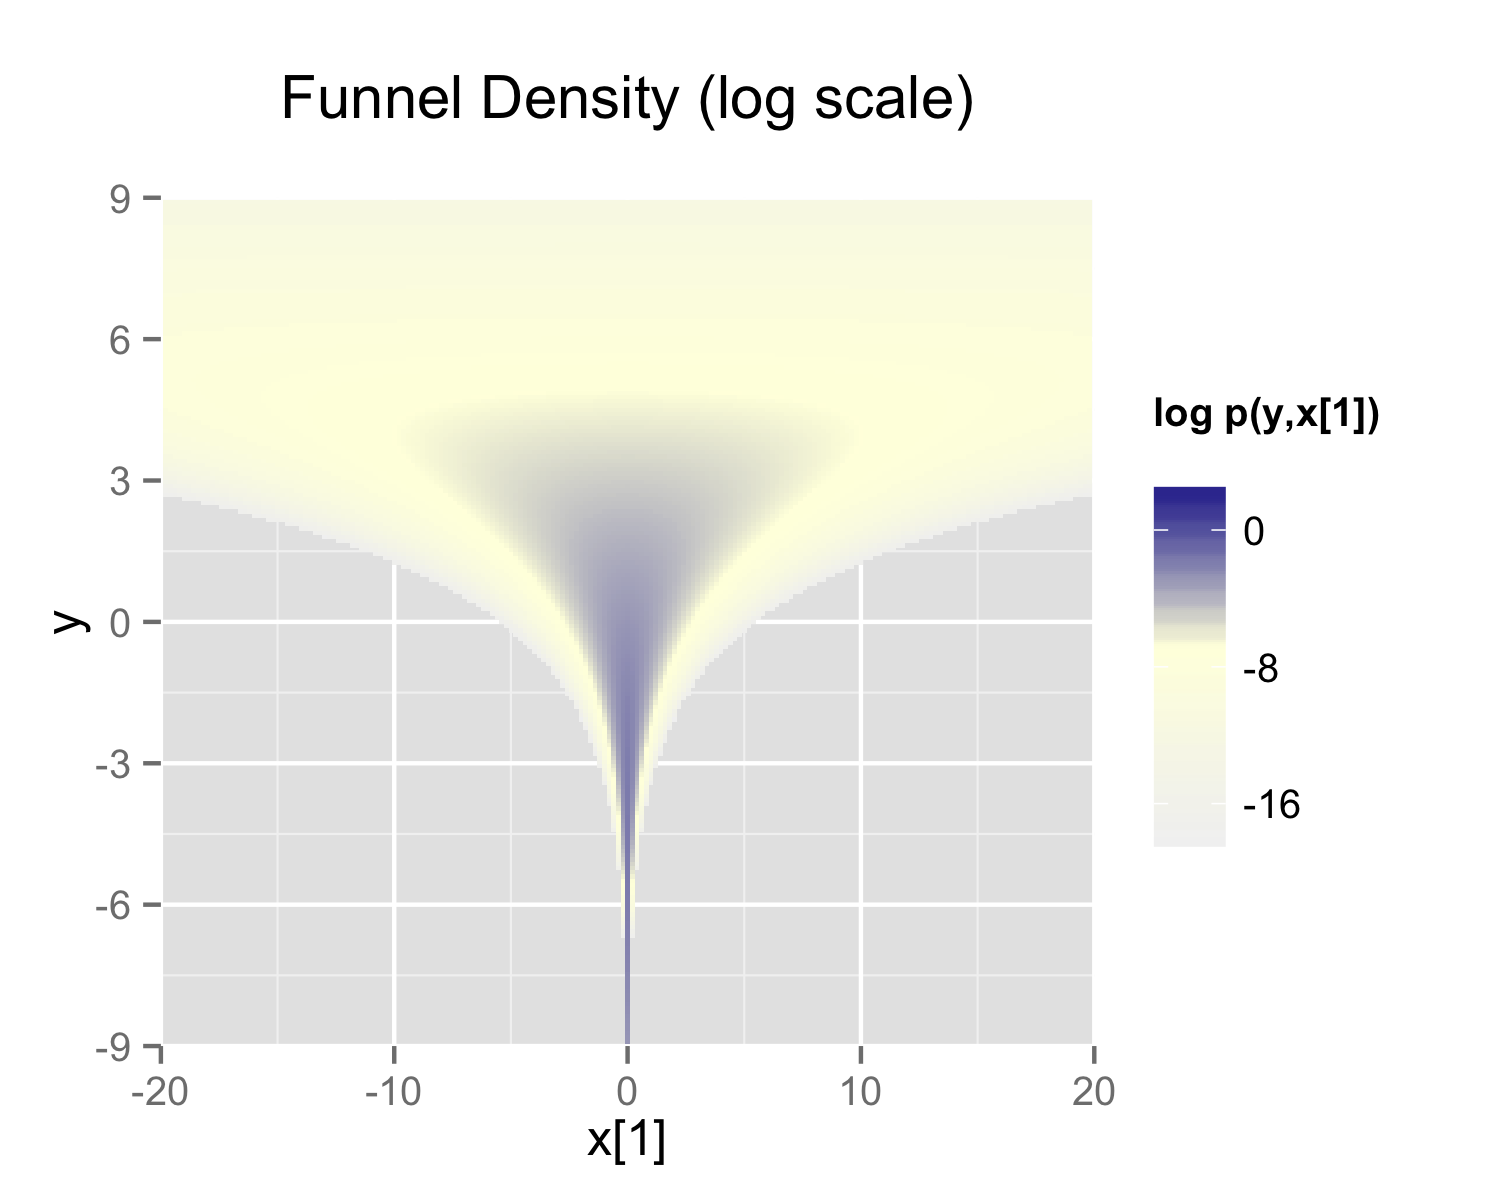
\includegraphics[height=2in]{R/funnel.png}
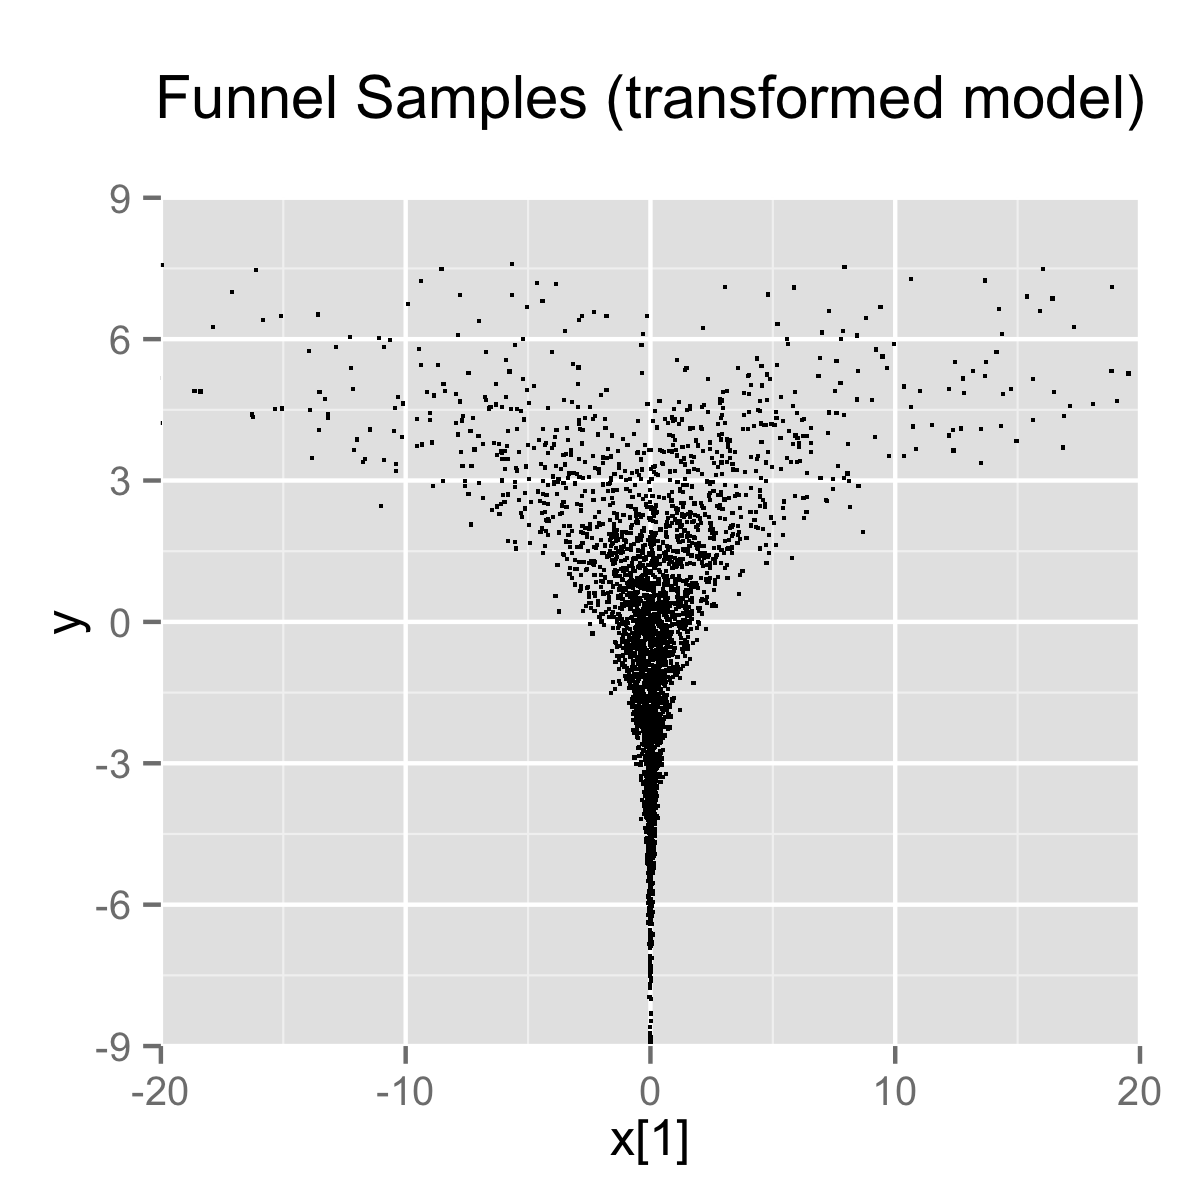
\includegraphics[height=2in]{R/funnel-fit.png}
\end{center}
\vspace*{-18pt}
\caption{\small \it Neal's Funnel.  (Left) The marginal density of
  Neal's funnel for the upper-level variable $y$ and one lower-level
  variable $x_1$ (see the text for the formula).  The blue region has
  log density greater than -8, the yellow region density greater than
  -16, and the gray background a density less than -16.  
  (Right) 4000 draws from a run of Stan's
  sampler with default settings.  Both plots are restricted to the
  shown window of $x_1$ and $y$ values; some draws fell outside of
  the displayed area as would be expected given the density.  The samples are
  consistent with the marginal density $p(y) =
  \distro{Normal}(y|0,3)$, which has mean 0 and standard deviation
  3.}\label{funnel.figure}
\end{figure}

\citep{Neal:2003} defines a distribution that exemplifies the
difficulties of sampling from some hierarchical models.  Neal's
example is fairly extreme, but can be trivially reparameterized in
such a way as to make sampling straightforward.

Neal's example has support for $y \in
\mathbb{R}$ and  $x \in \mathbb{R}^9$ with density
%
\[
p(y,x) = \distro{Normal}(y|0,3) \times \prod_{n=1}^9
\distro{Normal}(x_n|0,\exp(y/2)).
\]
%
The probability contours are shaped like ten-dimensional funnels.  The
funnel's neck is particularly sharp because of the exponential
function applied to $y$.  A plot of the log marginal density of $y$
and the first dimension $x_1$ is shown in \reffigure{funnel}.

The funnel can be implemented directly in Stan as follows.
%
\begin{quote}
\begin{Verbatim}[fontsize=\small]
parameters {  
  real y;
  vector[9] x;
}
model {
  y ~ normal(0,3);
  x ~ normal(0,exp(y/2));
}
\end{Verbatim}
\end{quote}
%
When the model is expressed this way, Stan has trouble sampling from
the neck of the funnel, where $y$ is small and thus $x$ is constrained
to be near 0.  This is due to the fact that the density's scale
changes with $y$, so that a step size that works well in the body will
be too large for the neck and a step size that works in the neck will be
very inefficient in the body.

In this particular instance, because the analytic form of the density
from which samples are drawn is known, the model can be converted to
the following more efficient form.
%
\begin{quote}
\begin{Verbatim}[fontsize=\small]
parameters {  
  real y_raw;
  vector[9] x_raw;
}
transformed parameters {
  real y;
  vector[9] x;

  y <- 3.0 * y_raw;  
  x <- exp(y/2) * x_raw;
}
model {
  y_raw ~ normal(0,1); // implies y ~ normal(0,3) 
  x_raw ~ normal(0,1); // implies x ~ normal(0,exp(y/2))  
}
\end{Verbatim}
\end{quote}
%
In this second model, the parameters \Verb|x_raw| and \Verb|y_raw| are
sampled as independent unit normals, which is easy for Stan.  These
are then transformed into samples from the funnel.  In this case, the
same transform may be used to define Monte Carlo samples directly
based on independent unit normal samples; Markov chain Monte Carlo
methods are not necessary. If such a reparameterization were used in
Stan code, it is useful to provide a comment indicating what the
distribution for the parameter implies for the distribution of the
transformed parameter.

\subsection{Reparameterizing the Cauchy}

Sampling from heavy tailed distributions such as the Cauchy is
difficult for Hamiltonian Monte Carlo, which operates within a
Euclidean geometry.%
\footnote{Riemannian Manifold Hamiltonian Monte Carlo (RMHMC) overcomes
  this difficulty by simulating the Hamiltonian dynamics in a a space
  with a position-dependent metric; see
  \citep{GirolamiCalderhead:2011} and \citep{Betancourt:2012}.}
%
The practical problem is that tail of the Cauchy
requires a relatively large step size compared to the trunk.  With a
small step size, the No-U-Turn sampler requires many steps when
starting in the tail of the distribution; with a large step size,
there will be too much rejection in the central portion of the
distribution.  This problem may be mitigated by defining the
Cauchy-distributed variable as the transform of a uniformly
distributed variable using the Cauchy inverse cumulative distribution
function.

Suppose a random variable of interest $X$ has a Cauchy distribution
with location $\mu$ and scale $\tau$, so that $X \sim
\distro{Cauchy}(\mu,\tau)$.  The variable $X$ has a cumulative
distribution function $F_X:\reals \rightarrow (0,1)$ defined by
\[
F_X(x) = \frac{1}{\pi} \arctan \left( \frac{x - \mu}{\tau} \right) +
\frac{1}{2}.
\]
The inverse of the cumulative distribution function,
$F_X^{-1}:(0,1) \rightarrow \reals$, is thus
%
\[
F^{-1}_X(y) = \mu + \tau \tan \left( \pi \left( x - \frac{1}{2} \right) \right).
\]
Thus if the random variable $Y$ has a unit uniform distribution, $Y
\sim \distro{Uniform}(0,1)$, then $F^{-1}_X(Y)$ has a Cauchy
distribution with location $\mu$ and scale $\tau$, i.e., $F^{-1}_X(Y) \sim
\distro{Cauchy}(\mu,\tau)$. 

Consider a Stan program involving a Cauchy-distributed parameter
\code{beta}.
%
\begin{quote}
\begin{Verbatim}[fontsize=\small]
parameters {
  real beta;
  ...
}
model {
  beta ~ cauchy(mu,tau);
  ...
}
\end{Verbatim}
\end{quote}
%
This declaration of \code{beta} as a parameter may be replaced with a
transformed parameter \code{beta} defined in terms of a
uniform-distributed parameter \code{beta\_unif}.
%
\begin{quote}
\begin{Verbatim}[fontsize=\small]
parameters {
  real<lower=-pi()/2, upper=pi()/2> beta_unif;
  ...
}
transformed parameters {
  real beta;
  beta <- mu + tau * tan(beta_unif);  // beta ~ cauchy(mu,tau)
}    
model {
  beta_unif ~ uniform(-pi()/2, pi()/2);  // not necessary
  ...
}
\end{Verbatim}
\end{quote}
%
It is more convenient in Stan to transform a uniform variable on
$(-\pi/2, \pi/2)$ than one on $(0,1)$.  The Cauchy location and scale
parameters, \code{mu} and \code{tau}, may be defined as data or may
themselves be parameters.  The variable \code{beta} could also be
defined as a local variable if it does not need to be included in the
sampler's output.

The uniform distribution on \code{beta\_unif} is defined explicitly in
the model block, but it could be safely removed from the program
without changing sampling behavior.  This is because $\log
\distro{Uniform}(\beta_{\mbox{\footnotesize unif}}|-\pi/2,\pi/2) =
-\log \pi$ is a constant and Stan only
needs the total log probability up to an additive constant.  Stan will spend
some time checking that that \code{beta\_unif} is between
\code{-pi()/2} and \code{pi()/2}, but this condition is guaranteed by
the constraints in the declaration of \code{beta\_unif}.  

\subsection{Reparameterizing a Student-t Distribution}

One thing that sometimes works when you're having trouble with the
heavy-tailedness of Student-t distributions is to use the
gamma-mixture representation, which says that you can generate a
Student-t distributed variable $\beta$,
\[
\beta \sim \mbox{\sf Student-t}(\nu, 0, 1),
\]
by first generating a gamma-distributed $\tau$,
\[
\tau \sim \mbox{\sf Gamma}(\nu/2, \nu/2),
\]
and then generating $\beta$ from the normal distribution with
precision $\tau$, which using our parameterization of the normal in
terms of scale, is
\[
\beta \sim \mbox{\sf Normal}(0,\tau^{-2}).
\]
%
That is, the marginal distribution of $\beta$ when you integrate out
$\tau$ is $\mbox{\sf Student-t}(\nu, 0, 1)$, i.e.,
\[
\mbox{\sf Student-t}(\beta | \nu,0,1).
= 
\int_0^{\infty} 
\,
\mbox{\sf Normal}(\beta | 0, 1 / \tau^{2}) 
\times
\mbox{\sf Gamma}(\tau | \nu/2, \nu/2)
\
d\tau.
\]
%
You can go a step further and instead of defining a $\beta$ drawn from
a normal with precision $\tau$, define $\alpha$ to be drawn from a
unit normal,
%
\[
\alpha \sim \mbox{\sf Normal}(0,1)
\]
%
and rescale by defining
%
\[
\beta = \alpha / \tau^{2}.
\]
%
Now suppose $\mu = \beta x$ is the product of $\beta$ with a
regression predictor $x$.  Then the reparameterization $\mu = \alpha
\tau^{-2} x$ has the same distribution, but in the original, direct
parameterization, $\beta$ has (potentially) heavy tails, whereas in
the second, neither $\tau$ nor $\alpha$ have heavy tails.

To translate into Stan notation, this reparameterization replaces
%
\begin{quote}
\begin{Verbatim}
parameters {
  real<lower=0> nu;
  real beta;
  ...
model {
  beta ~ student_t(nu,0,1);
  ...
\end{Verbatim}
\end{quote}
%
with
%
\begin{quote}
\begin{Verbatim}
parameters {
  real<lower=0> nu;
  real<lower=0> tau;
  ...
transformed parameters {
  real beta;
  beta <- alpha / pow(tau,2);
  ...
model {
  real half_nu;
  half_nu <- 0.5 * nu;
  tau ~ gamma(half_nu, half_nu);
  alpha ~ normal(0, 1);
  ...
\end{Verbatim}
\end{quote}  
%
In most cases, the lower bound for \code{nu} can be set to \code{1} or
higher; when \code{nu} is 1, the result is a Cauchy distribution with
very fat tails and as \code{nu} approaches infinity, the distribution
approaches a normal distribution.   So the model for \code{nu}
effectively parameterizes the heaviness of the tails of the model.

\subsection{Hierarchical Models}

Unfortunately, the usual situation in applied Bayesian modeling
involves complex geometries and interactions that are not known
analytically.  Nevertheless, reparameterization can still be very
effective for separating parameters.  For example, a vectorized
hierarchical model might draw a vector of coefficients $\beta$ with
definitions as follows.
%
\begin{quote}
\begin{Verbatim}[fontsize=\small]
parameters {
  real mu_beta;   
  real<lower=0> sigma_beta;
  vector[K] beta;
  ...
model {
  beta ~ normal(mu_beta,sigma_beta);
  ...
\end{Verbatim}
\end{quote}
%
Although not shown, a full model will have priors on both
\Verb|mu_beta| and \Verb|sigma_beta| along with data modeled based on
these coefficients.  For instance, a standard binary logistic
regression with data matrix \code{x} and binary outcome vector
\code{y} would include a likelihood statement such as form
\Verb|y ~ bernoulli_logit(x * beta)|, leading to an analytically
intractable posterior.

A hierarchical model such as the above will suffer from the same kind
of inefficiencies as Neal's funnel, though typically not so extreme,
because the values of \Verb|beta|, \Verb|mu_beta| and
\Verb|sigma_beta| are highly correlated in the posterior.  Such a
hierarchical model can be made much more efficient in terms of
effective sample size by reparameterizing in exactly the same way as
the funnel example.
%
\begin{quote}
\begin{Verbatim}[fontsize=\small]
parameters {
  vector[K] beta_raw;
  ...
transformed parameters {
  vector[K] beta;
  // implies: beta ~ normal(mu_beta,sigma_beta)
  beta <- mu_beta + sigma_beta * beta_raw;
model {
  beta_raw ~ normal(0,1);  
  ...
\end{Verbatim}
\end{quote}
%
Any priors defined for \Verb|mu_beta| and \Verb|sigma_beta| remain as
defined in the original model.

Reparameterization of hierarchical models is not limited to the normal
distribution, although the normal distribution is the best candidate
for doing so. In general, any distribution of parameters in the 
location-scale family is a good candidate for reparameterization. Let
$\beta = l + s\alpha$ where $l$ is a location parameter and $s$ is a
scale parameter. Note that $l$ need not be the mean, $s$ need not
be the standard deviation, and neither the mean nor the standard
deviation need to exist. If $\alpha$ and $\beta$ are from the same
distributional family but $\alpha$ has location zero and unit scale, 
while $\beta$ has location $l$ and scale $s$, then that distribution
is a location-scale distribution. Thus, if $\alpha$ were a parameter
and $\beta$ were a transformed parameter, then a prior distribution
from the location-scale family on $\alpha$ with location zero and unit 
scale implies a prior distribution on $\beta$ with location $l$ and
scale $s$. Doing so would reduce the dependence between $\alpha$, 
$l$, and $s$.

There are several univariate distributions in the location-scale
family, such as the Student t distribution, including its special
cases of the Cauchy distribution (with one degree of freedom) and the
normal distribution (with infinite degrees of freedom). As shown above,
if $\alpha$ is distributed standard normal, then $\beta$ is distributed
normal with mean $\mu = l$ and standard deviation $\sigma = s$. The 
logistic, the double exponential, the generalized extreme value 
distributions, and the stable distribution are also in the 
location-scale family.

Also, if $z$ is distributed standard normal, then $z^2$ is distributed
chi-squared with one degree of freedom. By summing the squares of $K$
independent standard normal variates, one can obtain a single variate
that is distributed chi-squared with $K$ degrees of freedom. However,
for large $K$, the computational gains of this reparameterization may
be overwhelmed by the computational cost of specifying $K$ primitive
parameters just to obtain one transformed parameter to use in a model.

\subsection{Multivariate Reparameterizations}

The benefits of reparameterization are not limited to univariate 
distributions. A parameter with a multivariate normal prior distribution
is also an excellent candidate for reparameterization. Suppose you intend
the prior for $\beta$ to be multivariate normal with mean vector $\mu$
and covariance matrix $\Sigma$. Such a belief is reflected by the
following code.
%
\begin{quote}
\begin{Verbatim}[fontsize=\small]
data {
  int<lower=2> K;
  vector[K] mu;
  cov_matrix[K] Sigma;
  ...
parameters {
  vector[K] beta;
  ...
model {
  beta ~ multi_normal(mu,Sigma);
  ...
\end{Verbatim}
\end{quote}
%
In this case \Verb|mu| and \Verb|Sigma| are fixed data, but they could
be unknown parameters, in which case their priors would be unaffected
by a reparameterization of \Verb|beta|.

If $\alpha$ has the same dimensions as $\beta$ but the elements of 
$\alpha$ are independently and identically distributed standard normal 
such that $\beta = \mu + L\alpha$, where $LL^\top = \Sigma$, then 
$\beta$ is distributed multivariate normal with mean vector $\mu$ and 
covariance matrix $\Sigma$. One choice for $L$ is the Cholesky factor
of $\Sigma$. Thus, the model above could be reparameterized as follows.
%
\begin{quote}
\begin{Verbatim}[fontsize=\small]
data {
  int<lower=2> K;
  vector[K] mu;
  cov_matrix[K] Sigma;
  ...
transformed data {
  matrix[K,K] L;
  L <- cholesky_decompose(Sigma);
}
parameters {
  vector[K] alpha;
  ...
transformed parameters {
  vector[K] beta;
  beta <- mu + L * alpha; 
}
model {
  alpha ~ normal(0,1); 
  // implies: beta ~ multi_normal(mu, Sigma)
  ...
\end{Verbatim}
\end{quote}
%
This reparameterization is more efficient for two reasons. First, it
reduces dependence among the elements of \Verb|alpha| and second, it
avoids the need to invert \Verb|Sigma| every time \Verb|multi_normal|
is evaluated.

The Cholesky factor is also useful when a covariance matrix is 
decomposed into a correlation matrix that is multiplied from both
sides by a diagonal matrix of standard deviations, where either the
standard deviations or the correlations are unknown parameters. The
Cholesky factor of the covariance matrix is equal to the product of
a diagonal matrix of standard deviations and the Cholesky factor of
the correlation matrix. Furthermore, the product of a diagonal matrix
of standard deviations and a vector is equal to the elementwise
product between the standard deviations and that vector. Thus, if for
example the correlation matrix \Verb|Tau| were fixed data but the
vector of standard deviations \Verb|sigma| were unknown parameters,
then a reparameterization of \Verb|beta| in terms of \Verb|alpha|
could be implemented as follows.
%
\begin{quote}
\begin{Verbatim}[fontsize=\small]
data {
  int<lower=2> K;
  vector[K] mu;
  corr_matrix[K] Tau;
  ...
transformed data {
  matrix[K,K] L;
  L <- cholesky_decompose(Tau);
}
parameters {
  vector[K] alpha;
  vector<lower=0>[K] sigma;
  ...
transformed parameters {
  vector[K] beta;
  // This equals mu + diag_matrix(sigma) * L * alpha;
  beta <- mu + sigma .* (L * alpha);
}
model {
  sigma ~ cauchy(0,5);
  alpha ~ normal(0,1);
  // implies: beta ~ multi_normal(mu,
  //  diag_matrix(sigma) * L * L' * diag_matrix(sigma)))
  ...
\end{Verbatim}
\end{quote}
%
This reparameterization of a multivariate normal distribution in
terms of standard normal variates can be extended to other multivariate
distributions that can be conceptualized as contaminations of the 
multivariate normal, such as the multivariate Student t and the skew
multivariate normal distribution.

A Wishart distribution can also be reparameterized in terms of standard
normal variates and chi-squared variates. Let $L$ be the Cholesky factor
of a $K \times K$ positive definite scale matrix $S$ and let $\nu$ be
the degrees of freedom. If
\begin{equation*}
A = \left( \begin{array}{cccc}
\sqrt{c_{1}} & 0 & \cdots & 0\\
z_{21} & \sqrt{c_{2}} & \ddots & \vdots\\
\vdots & \ddots & \ddots & 0\\
z_{K1} & \cdots & z_{K\left(K-1\right)} & \sqrt{c_{K}}
 \end{array} \right),
\end{equation*}
where each $c_i$ is distributed chi-squared with $\nu - i + 1$ degrees
of freedom and each $z_{ij}$ is distributed standard normal, then
$W = LAA^{\top}L^{\top}$ is distributed Wishart with scale matrix
$S = LL^{\top}$ and degrees of freedom $\nu$. Such a reparameterization
can be implemented by the following Stan code:
%
\begin{quote}
\begin{Verbatim}[fontsize=\small]
data {
  int<lower=1> N;
  int<lower=1> K;
  int<lower=K+2> nu
  matrix[K,K] L; // Cholesky factor of scale matrix
  vector[K] mu;
  matrix[N,K] y;
  ...
parameters {
  vector<lower=0>[K] c;
  vector[0.5 * K * (K - 1)] z;
  ...
model {
  matrix[K,K] A;
  int count;
  count <- 1;
  for (j in 1:(K-1)) {
    for (i in (j+1):K) {
      A[i,j] <- z[count];
      count <- count + 1;
    }
    for (i in 1:(j - 1)) {
      A[i,j] <- 0.0;
    }
    A[j,j] <- sqrt(c[j]);
  }
  
  for (i in 1:K) {
    c[i] ~ chi_square(nu - i + 1);
  }
  z ~ normal(0,1);
  // implies: L * A * A' * L' ~ wishart(nu, L * L')
  y ~ multi_normal_cholesky(mu, L * A);
  ...
\end{Verbatim}
\end{quote}
%
This reparameterization is more efficient for three reasons. First, it
reduces dependence among the elements of \Verb|z| and second, it
avoids the need to invert the covariance matrix, $W$ every time 
\Verb|wishart| is evaluated. Third, if $W$ is to be used with a
multivariate normal distribution, you can pass $L A$ to the more
efficient \Verb|multi_normal_cholesky| function, rather than passing
$W$ to \Verb|multi_normal|.

If $W$ is distributed Wishart with scale matrix $S$ and degrees of
freedom $\nu$, then $W^{-1}$ is distributed inverse Wishart with inverse
scale matrix $S^{-1}$ and degrees of freedom $\nu$. Thus, the previous
result can be used to reparameterize the inverse Wishart distribution.
Since $W = L * A * A^{\top} * L^{\top}$, 
$W^{-1} = L^{{\top}^{-1}} A^{{\top}^{-1}} A^{-1} L^{-1}$, where all four
inverses exist, but 
$L^{{-1}^{\top}} = L^{{\top}^{-1}}$ and $A^{{-1}^{\top}} = A^{{\top}^{-1}}$.
We can slightly modify the above Stan code for this case:
%
\begin{quote}
\begin{Verbatim}[fontsize=\small]
data {
  int<lower=1> K;
  int<lower=K+2> nu
  matrix[K,K] L; // Cholesky factor of scale matrix
  ...
transformed data {
  matrix[K,K] eye;
  matrix[K,K] L_inv;
  for (j in 1:K) {
    for (i in 1:K) {
      eye[i,j] <- 0.0;
    }
    eye[j,j] <- 1.0;
  }
  L_inv <- mdivide_left_tri_low(L, eye);
}
parameters {
  vector<lower=0>[K] c;
  vector[0.5 * K * (K - 1)] z;
  ...
model {
  matrix[K,K] A;
  matrix[K,K] A_inv_L_inv;  
  int count;
  count <- 1;
  for (j in 1:(K-1)) {
    for (i in (j+1):K) {
      A[i,j] <- z[count];
      count <- count + 1;
    }
    for (i in 1:(j - 1)) {
      A[i,j] <- 0.0;
    }
    A[j,j] <- sqrt(c[j]);
  }
  A_inv_L_inv <- mdivide_left_tri_low(A, L_inv);
  for (i in 1:K) {
    c[i] ~ chi_square(nu - i + 1);
  }
  z ~ normal(0,1); // implies: crossprod(A_inv_L_inv) ~ 
  // inv_wishart(nu, L_inv' * L_inv)
  ...
\end{Verbatim}
\end{quote}
%
Another candidate for reparameterization is the Dirichlet distribution
with all $K$ shape parameters equal. \cite{ZyczkowskiSommers:2001} shows 
that if $\theta_i$ is equal to the sum of $\beta$ independent squared 
standard normal variates and $\rho_i = \frac{\theta_i}{\sum \theta_i}$, 
then the $K$-vector $\rho$ is distributed Dirichlet with all shape 
parameters equal to $\frac{\beta}{2}$. In particular, if $\beta = 2$, 
then $\rho$ is distributed uniformally on the unit simplex. Thus, we can 
make $\rho$ be a transformed parameter to reduce dependence, as in:
%
\begin{quote}
\begin{Verbatim}[fontsize=\small]
data {
  int<lower=1> beta;
  ...
parameters {
  vector[beta] z[K];
  ...
transformed parameters {
  simplex[K] rho;
  for (k in 1:K)
    rho[k] <- dot_self(z[k]); // sum-of-squares
  rho <- rho / sum(rho);
}
model {
  for (k in 1:K)
    z[k] ~ normal(0,1); 
  // implies: rho ~ dirichlet(0.5 * beta * ones)
  ...
\end{Verbatim}
\end{quote}
%

\section{Vectorization}

\subsection{Gradient Bottleneck}

\Stan spends the vast majority of its time computing the gradient of
the log probability function, making gradients the obvious target for
optimization.  \Stan's gradient calculations with algorithmic
differentiation require a template expression to be allocated%
%
\footnote{\Stan uses its own arena-based allocation, so allocation and
  deallocation are faster than with a raw call to \code{new}.}
%
and constructed for each subexpression of a \Stan program involving
parameters or transformed parameters.  This section defines
optimization strategies based on vectorizing these subexpressions to
reduce the work done during algorithmic differentiation.

\subsection{Vectorizing Summations}

Because of the gradient bottleneck described in the previous section,
it is more efficient to collect a sequence of summands into a vector
or array and then apply the \code{sum()} operation than it is to
continually increment a variable by assignment and addition.  For
example, consider the following code snippet, where \code{foo()} is
some operation that depends on \code{n}.
%
\begin{quote}
\begin{Verbatim}[fontsize=\small]
for (n in 1:N) 
  total <- total + foo(n,...);
\end{Verbatim}
\end{quote}
%
This code has to create intermediate representations for each
of the \code{N} summands.  

A faster alternative is to copy the values into a vector, then
apply the \code{sum()} operator, as in the following refactoring.
%
\begin{quote}
\begin{Verbatim}[fontsize=\small]
{  
  vector[N] summands;
  for (n in 1:N) 
    summands[n] <- foo(n,...);
  total <- sum(summands);
}
\end{Verbatim}
\end{quote}
%
Syntactically, the replacement is a statement block delineated
by curly brackets (\Verb|{|, \Verb|}|), starting with the definition
of the local variable \code{summands}.

Even though it involves extra work to allocate the \code{summands}
vector and copy \code{N} values into it, the savings in
differentiation more than make up for it.  Perhaps surprisingly,
it will also use substantially less memory overall than incrementing
\code{total} within the loop.


\subsection{Vectorization through Matrix Operations}

The following program directly encodes a linear regression with fixed
unit noise using a two-dimensional array \code{x} of predictors, an
array \code{y} of outcomes, and an array \code{beta} of regression
coefficients.
%
\begin{quote}
\begin{Verbatim}[fontsize=\small]
data {
  int<lower=1> K;
  int<lower=1> N;
  real x[K,N];
  real y[N];
}
parameters {
  real beta[K];
}
model {
  for (n in 1:N) {
    real gamma;  
    gamma <- 0.0;
    for (k in 1:K)
      gamma <- gamma + x[n,k] * beta[k];
    y[n] ~ normal(gamma,1);
  }
}
\end{Verbatim}
\end{quote}
%
The following model computes the same log probability function as the
previous model, even supporting the same input files for data and
initialization.
%
\begin{quote}
\begin{Verbatim}[fontsize=\small]
data {
  int<lower=1> K;
  int<lower=1> N;
  vector[K] x[N];
  real y[N];
}
parameters {
  vector[K] beta;
}
model {
  for (n in 1:N)
    y[n] ~ normal(dot_product(x[n],beta), 1);
}
\end{Verbatim}
\end{quote}
%
Although it produces equivalent results, the dot product should not be
replaced with a transpose and multiply, as in
%
\begin{quote}
\begin{Verbatim}[fontsize=\small]
        y[n] ~ normal(x[n]' * beta, 1);
\end{Verbatim}
\end{quote}
%
The relative inefficiency of the transpose and multiply approach is
that the transposition operator allocates a new vector into which the
result of the transposition is copied.  This consumes both time
and memory\footnote{Future versions of \Stan may remove this inefficiency
by more fully exploiting expression templates inside the Eigen
\Cpp matrix library.  This will require enhancing Eigen to deal
with mixed-type arguments, such as the type \code{double} used
for constants and the algorithmic differentiation type
\code{stan::agrad::var} 
used for variables.}.
%
The inefficiency of transposition could itself be mitigated somewhat by
reordering the product and pulling the transposition out of the loop,
as follows.
%
\begin{quote}
\begin{Verbatim}[fontsize=\small]
...
transformed parameters {
  row_vector[K] beta_t;
  beta_t <- beta';
}
model {
  for (n in 1:N)
    y[n] ~ normal(beta_t * x[n], 1);
}
\end{Verbatim}
\end{quote}
%
The problem with transposition could be completely solved by directly
encoding the \code{x} as a row vector, as in the
following example.
%
\begin{quote}
\begin{Verbatim}[fontsize=\small]
data {
  ...
  row_vector[K] x[N];
  ...
}
parameters {
  vector[K] beta;
}
model {
  for (n in 1:N)
    y[n] ~ normal(x[n] * beta, 1);
}
\end{Verbatim}
\end{quote}
%
Declaring the data as a matrix and then computing all the predictors
at once using matrix multiplication is more efficient still, as in the
example discussed in the next section.

\subsection{Vectorized Probability Functions}

The final and most efficient version replaces the loops and
transformed parameters by using the vectorized form of the normal
probability function, as in the following example.
%
\begin{quote}
\begin{Verbatim}[fontsize=\small]
data {
  int<lower=1> K;
  int<lower=1> N;
  matrix[N,K] x;
  vector[N] y;
}
parameters {
  vector[K] beta;
} 
model {
  y ~ normal(x * beta, 1);
}
\end{Verbatim}
\end{quote}
%
The variables are all declared as either matrix or vector types.
The result of the matrix-vector multiplication \code{x * beta} in the
model block is a vector of the same length as \code{y}.  

The probability function documentation in \refpart{built-in-functions}
indicates which of \Stan's probability functions support
vectorization; see \refsection{prob-vectorization} for more
information.  Vectorized probability functions accept either vector or
scalar inputs for all arguments, with the only restriction being that
all vector arguments are the same dimensionality.  In the example
above, \code{y} is a vector of size \code{N}, \code{x * beta} is a
vector of size \code{N}, and \code{1} is a scalar.

\section{Exploiting Sufficient Statistics}

In some cases, models can be recoded to exploit sufficient statistics
in estimation.  This can lead to large efficiency gains compared to an
expanded model.  For example, consider the following Bernoulli
sampling model.
%
\begin{quote}
\begin{Verbatim}[fontsize=\small]
data {
  int<lower=0> N;
  int<lower=0,upper=1> y[N];
  real<lower=0> alpha;
  real<lower=0> beta;
}
parameters {
  real<lower=0,upper=1> theta;
}
model {
  theta ~ beta(alpha,beta);
  for (n in 1:N) 
    y[n] ~ bernoulli(theta);
}
\end{Verbatim}
\end{quote}
%
In this model, the sum of positive outcomes in \code{y} is a
sufficient statistic for the chance of success \code{theta}.  The
model may be recoded using the binomial distribution as follows.
%
\begin{quote}
\begin{Verbatim}[fontsize=\small]
    theta ~ beta(alpha,beta);
    sum(y) ~ binomial(N,theta);
\end{Verbatim}
\end{quote}
%
Because truth is represented as one and falsehood as zero, the sum
\code{sum(y)} of a binary vector \code{y} is equal to the number of
positive outcomes out of a total of \code{N} trials.  



\section{Exploiting Conjugacy}


Continuing the model from the previous section, the conjugacy of the
beta prior and binomial sampling distribution allow the model to be
further optimized to the following equivalent form.
%
\begin{quote}
\begin{Verbatim}[fontsize=\small]
    theta ~ beta(alpha + sum(y), beta + N - sum(y));
\end{Verbatim}
\end{quote}
%
To make the model even more efficient, a transformed data variable
defined to be \code{sum(y)} could be used in the place of \code{sum(y)}.

\section{Standardizing Predictors and Outputs}

Stan programs will run faster if the input is standardized to have a
zero sample mean and unit sample variance.  This section illustrates
the principle with a simple linear regression.

Suppose that $y = (y_1,\ldots,y_N)$ is a sequence of $N$ outcomes and
$x = (x_1,\ldots,x_N)$ a parallel sequence of $N$ predictors.  A
simple linear regression involving an intercept coefficient $\alpha$
and slope coefficient $\beta$ can be expressed as
\[
y_n = \alpha + \beta x_n + \epsilon_n,
\]
where
\[
\epsilon_n \sim \distro{Normal}(0,\sigma).
\]

If either vector $x$ or $y$ has very large or very small values or if the
sample mean of the values is far away from 0 (on the scale of the values),
then it can be more efficient to standardize the outputs $y_n$ and
predictors $x_n$.  The data is first centered by subtracting the
sample mean, and then scaled by dividing by the sample deviation.
Thus a data point $u$ is standardized is standardized with respect to
a vector $y$  by the function $\mbox{z}_y$, defined by
\[
\mbox{z}_y(u) = \frac{u - \bar{y}}{\mbox{sd}(y)}
\]
where the sample mean of $y$ is
\[
\bar{y}
= \frac{1}{N} \sum_{n=1}^N y_n,
\]
and the sample standard deviation of $y$ is
\[
\mbox{sd}(y) 
= \left( 
\frac{1}{N} \sum_{n=1}^N (y_n - \bar{y})^2
\right)^{1/2}.
\]
The inverse transform is
defined by reversing the two normalization steps, first rescaling by
the same deviation and relocating by the sample mean,
\[
\mbox{z}^{-1}(v) = \mbox{sd}(y) v + \bar{y}.
\]

To standardize a regression problem, the predictors and outcomes are
standardized.  This changes the scale of the variables, and hence
changes the scale of the priors.  Consider the following initial
model.
%
\begin{quote}
\begin{Verbatim}[fontsize=\small]
data {
  int<lower=0> N;
  vector[N] y;
  vector[N] x;
}
parameters {
  real alpha;
  real beta;
  real<lower=0> sigma;
}
model {
  // priors
  alpha ~ normal(0,10);    
  beta ~ normal(0,10);
  sigma ~ cauchy(0,5);
  // likelihood
  for (n in 1:N)
    y[n] ~ normal(alpha + beta * x[n], sigma);
}
\end{Verbatim}
\end{quote}
%

The data block for the standardized model is identical.  The
standardized predictors and outputs are defined in the transformed
data block.  
%
\begin{quote}
\begin{Verbatim}[fontsize=\small]
data {
  int<lower=0> N;
  vector[N] y;
  vector[N] x;
}
transformed data {
  vector[N] x_std;
  vector[N] y_std;
  x_std <- (x - mean(x)) / sd(x);
  y_std <- (y - mean(y)) / sd(y);
}
parameters {
  real alpha_std;
  real beta_std;
  real<lower=0> sigma_std;
}
model {
  alpha_std ~ normal(0,10);    
  beta_std ~ normal(0,10);
  sigma_std ~ cauchy(0,5);
  for (n in 1:N)
    y_std[n] ~ normal(alpha_std + beta_std * x_std[n], 
                      sigma_std);
}
\end{Verbatim}
\end{quote}
%
The parameters are renamed to indicate that they aren't the
``natural'' parameters, but the model is otherwise identical.  In
particular, the fairly diffuse priors on the coefficients and error
scale are the same.  These could have been transformed as well, but
here they are left as is, because the scales make sense as very
diffuse priors for standardized data; the priors could be made more
informative.  For instance, because the outputs $y$ have been
standardized, the error $\sigma$ should not be greater than 1, because
that's the scale of the noise for predictors $\alpha = \beta = 0$.

The original regression
\[
y_n 
= \alpha + \beta x_n + \epsilon_n
\]
has been transformed to a regression on the standardized variables,
\[
\mbox{z}_y(y_n)
= \alpha'
+ \beta' \mbox{z}_x(x_n)
+ \epsilon'_n.
\]
The original parameters can be recovered with a little algebra,
%
\begin{eqnarray*}
y_n 
& = & \mbox{z}_y^{-1}(\mbox{z}_y(y_n))
\\[4pt]
& = & 
\mbox{z}_y^{-1} 
\left( 
\alpha' 
+ \beta' \mbox{z}_x(x_n)
+ \epsilon_n'
\right)
\\[4pt]
& = & 
\mbox{z}_y^{-1} 
\left( 
\alpha' 
+ \beta' 
    \left(  
      \frac{x_n - \bar{x}}{\mbox{\small sd}(x)}
    \right)
+ \epsilon_n'
\right)
\\[4pt]
& = & 
\mbox{sd}(y)
\left( 
\alpha' 
+ \beta' 
    \left(  
      \frac{x_n - \bar{x}}{\mbox{\small sd}(x)}
    \right)
+ \epsilon_n'
\right)
+ \bar{y}
\\[4pt]
& = & 
\left( 
  \mbox{sd}(y) 
      \left( 
          \alpha' 
          - \beta' \frac{\bar{x}}{\mbox{\small sd}(x)}
      \right) 
  + \bar{y}  
\right)
+ \left(
      \beta' \frac{\mbox{\small sd}(y)}{\mbox{\small sd}(x)} 
  \right) x_n
+ \mbox{sd}(y) \epsilon'_n,
\end{eqnarray*}
%
from which the original scale parameter values can be read off,
\[
\alpha 
=
\mbox{sd}(y) 
      \left( 
          \alpha' 
          - \beta' \frac{\bar{x}}{\mbox{\small sd}(x)}
      \right) 
  + \bar{y};
\ \ \ \ \ 
\beta = \beta' \frac{\mbox{\small sd}(y)}{\mbox{\small sd}(x)};
\ \ \ \ \
\sigma = \mbox{sd}(y) \sigma'.
\]
%
These recovered parameter values on the original scales can be
calculated within Stan using a generated quantities block following
the model block,
\begin{quote}
\begin{Verbatim}[fontsize=\small]
generated quantities {
  real alpha;
  real beta;
  real<lower=0> sigma;
  alpha <- sd(y) * (alpha_std - beta_std * mean(x) / sd(x)) 
           + mean(y);
  beta <- beta_std * sd(y) / sd(x);
  sigma <- sd(y) * sigma_std;
}
\end{Verbatim}
\end{quote}
%
Of course, it is inefficient to compute all of the means and standard
deviations every iteration; for more efficiency, these can be
calculated once and stored as transformed data.  Furthermore, the
model sampling statement can be easily vectorized, for instance, in
the transformed model, to
\begin{quote}
\begin{Verbatim}[fontsize=\small]
    y_std ~ normal(alpha_std + beta_std * x_std, sigma_std);
\end{Verbatim}
\end{quote}






% \section{Using Forward Sampling}

% In fact, at this point, simple (non Markov chain) Monte Carlo may be
% used because the parameters to the beta distribution are specified and
% there are no variables that depend on \code{theta}.  Thus this model
% could be even further optimized by replacing the declaration of
% \code{theta} as a parameter with a declaration as a generated quantity
% and then generating the quantity directly.
% %
% \begin{quote}
% \begin{Verbatim}
% generated quantities {
%     real<lower=0,upper=1> theta;
%     theta ~ random_beta(alpha + sum(y), beta + N - sum(y));
% }
% \end{Verbatim}
% \end{quote}
% %
% When used in the generated quantities block, sampling statements such
% as that for \code{theta} are executed by taking a sample from the
% specified distribution directly. The result is a Monte Carlo estimate
% of \code{theta} in which every sample is independent (up to the limits
% of the pseudorandom number generator, of course).  Thus the effective
% sample size should be estimated as being roughly equal to the sample
% size.

\part{Inference}

\chapter{Bayesian Data Analysis}\label{bayesian.chapter}

\noindent
\cite{GelmanEtAl:2013} provide the following
characterization of Bayesian data analysis.
%
\begin{quote}
  By Bayesian data analysis, we mean practical methods for making
  inferences from data using probability models for quantities we
  observe and about which we wish to learn.
\end{quote}
%
They go on to describe how Bayesian statistics differs from
frequentist approaches.
%
\begin{quote}
  The essential characteristic of Bayesian methods is their explicit
  use of probability for quantifying uncertainty in inferences based
  on statistical analysis.
\end{quote}
%
Because they view probability as the limit of relative frequencies of
observations, strict frequentists forbid probability statements about
parameters.  Parameters are considered fixed, not random.

Bayesians also treat parameters as fixed but unknown.  But unlike
frequentists, they make use of both prior distributions over
parameters and posterior distributions over parameters.  These prior
and posterior probabilities and posterior predictive probabilities are
intended to characterize knowledge about the parameters and future
observables.  Posterior distributions form the basis of Bayesian
inference, as described below.

\section{Bayesian Modeling}

\citep{GelmanEtAl:2013} break applied Bayesian modeling
into the following three steps.
%
\begin{enumerate}
\item  Set up a full probability model for all observable and
  unobservable quantities.  This model should be consistent with
  existing knowledge of the data being modeled and how it was
  collected.
\item Calculate the posterior probability of unknown quantities
  conditioned on observed quantities.  The unknowns may include
  unobservable quantities such as parameters and potentially
  observable quantities such as predictions for future observations.
\item Evaluate the model fit to the data.  This includes evaluating
  the implications of the posterior.
\end{enumerate}
%
Typically, this cycle will be repeated until a sufficient fit is
achieved in the third step.  Stan automates the calculations involved
in the second and third steps.

\section{Bayesian Inference}

\subsection{Basic Quantities}

The mechanics of Bayesian inference follow directly from Bayes's rule.
To fix notation, let $y$ represent observed quantities such as data
and let $\theta$ represent unknown quantities such as parameters and
future observations.  Both $y$ and $\theta$ will be modeled as random.
Let $x$ represent known, but unmodeled quantities such as constants,
hyperparameters, and predictors.

\subsection{Probability Functions}

The probability function $p(y,\theta)$ is the joint probability
function of the data $y$ and parameters $\theta$.  The constants and
predictors $x$ are implicitly understood as being part of the
conditioning.  The conditional probability function $p(y|\theta)$ of
the data $y$ given parameters $\theta$ and constants $x$ is called the
sampling probability function; it is also called the likelihood
function when viewed as a function of $\theta$ for fixed $y$ and $x$.

The probability function $p(\theta)$ over the parameters given the
constants $x$ is called the prior because it characterizes the probability
of the parameters before any data is observed.  The conditional
probability function $p(\theta|y)$ is called the posterior because
it characterizes the probability of parameters given observed data $y$
and constants $x$.

\subsection{Bayes's Rule}

The technical apparatus of Bayesian inference hinges on the following
chain of equations, known in various forms as Bayes's rule (where
again, the constants $x$ are implicit).
%
\[
\begin{array}{rcll}
p(\theta|y)  & =  & \displaystyle \frac{p(\theta,y)}{p(y)}
& \mbox{{} \ \ \ \ \ [definition of  conditional probability]}
\\[16pt]
& = & \displaystyle \frac{p(y|\theta) \, p(\theta)}{p(y)}
& \mbox{{} \ \ \ \ \ [chain rule]}
\\[16pt]
& = & \displaystyle \frac{p(y|\theta) \, p(\theta)}
                        {\int_{\Theta} p(y,\theta) \, d\theta}
& \mbox{{} \ \ \ \ \ [law of total probability]}
\\[16pt]
& = & \displaystyle \frac{p(y|\theta) \, p(\theta)}
                        {\int_{\Theta} p(y|\theta) \, p(\theta) \, d\theta}
& \mbox{{} \ \ \ \ \ [chain rule]}
\\[16pt]
& \propto & \displaystyle p(y|\theta) \, p(\theta)
& \mbox{{} \ \ \ \ \ [$y$ is fixed]}
\end{array}
\]
%
Bayes's rule ``inverts'' the probability of the posterior
$p(\theta|y)$, expressing it solely in terms of the likelihood
$p(y|\theta)$ and prior $p(\theta)$ (again, with constants and
predictors $x$ implicit).  The last step is important for Stan, which
only requires probability functions to be characterized up to a
constant multiplier.

\subsection{Predictive Inference}

The uncertainty in the estimation of parameters $\theta$ from the data
$y$ (given the model) is characterized by the posterior $p(\theta|y)$.
The posterior is thus crucial for Bayesian predictive inference.

If $\tilde{y}$ is taken to represent new, perhaps as yet unknown,
observations, along with corresponding constants and predictors
$\tilde{x}$, then the posterior predictive probability function is
given by
%
\[
p(\tilde{y}|y)
= \int_{\Theta} p(\tilde{y}|\theta)
                \, p(\theta|y) \, d\theta.
\]
Here, both the original constants and predictors $x$ and the new
constants and predictors $\tilde{x}$ are implicit.  Like the posterior
itself, predictive inference is characterized probabilistically.
Rather than using a point estimate of the parameters $\theta$,
predictions are made based on averaging the predictions over a range
of $\theta$ weighted by the posterior probability $p(\theta|y)$ of
$\theta$ given data $y$ (and constants $x$).

The posterior may also be used to estimate event probabilities.  For
instance, the probability that a parameter $\theta_k$ is greater than
zero is characterized probabilistically by
%
\[
\mbox{Pr}[\theta_k > 0]
= \int_{\Theta} \mbox{I}(\theta_k > 0) \, p(\theta|y) \, d\theta.
\]
%
The indicator function, $\mbox{I}(\phi)$, evaluates to one if the
proposition $\phi$ is true and evaluates to zero otherwise.

Comparisons involving future observables may be carried out in
the same way.  For example, the probability that $\tilde{y}_n >
\tilde{y}_{n'}$ can be characterized using the posterior predictive
probability function as
\[
\mbox{Pr}[\tilde{y}_n > \tilde{y}_{n'}]
= \int_{\Theta} \int_{Y} \mbox{I}(\tilde{y}_n > \tilde{y}_{n'}) \,
p(\tilde{y}|\theta) p(\theta|y) \, d\tilde{y} \, d\theta.
\]


\subsection{Posterior Predictive Checking}

After the parameters are fit to data, they can be used to simulate a
new data set by running the model inferences in the forward
direction.  These replicated data sets can then be compared to the
original data either visually or statistically to assess model fit
\citep[Chapter 6]{GelmanEtAl:2013}.

In Stan, posterior simulations can be generated in two ways.  The
first approach is to treat the predicted variables as parameters and
then define their distributions in the model block.  The second
approach, which also works for discrete variables, is to generate
replicated data using random-number generators in the generated
quantities block.



\chapter{Markov Chain Monte Carlo Sampling}\label{mcmc.chapter}

\noindent
Stan uses Markov chain Monte Carlo (\MCMC) techniques to
generate samples from the posterior distribution for inference.


\section{Monte Carlo Sampling}

Monte Carlo methods were developed to numerically approximate
integrals that are not tractable analytically but for which evaluation
of the function being integrated is tractable
\citep{MetropolisUlam:1949}.

For example, the mean $\mu$ of a probability density $p(\theta)$ is
defined by the integral
\[
\mu = \int_{\Theta} \, \theta \times p(\theta) \, d\theta.
\]
For even a moderately complex Bayesian model, the posterior density
$p(\theta|y)$ leads to an integral that is impossible to evaluate
analytically.  The posterior also depends on the constants and
predictors $x$, but from here, they will just be elided and taken as
given.

Now suppose it is possible to draw independent samples from
$p(\theta)$ and let $\theta^{(1)},\theta^{(2)},\ldots,\theta^{(N)}$ be
$N$ such samples.  A Monte Carlo estimate $\hat{\mu}$ of the mean
$\mu$ of $p(\theta)$ is given by the sample average,
\[
\hat{\mu} = \frac{1}{N} \sum_{n=1}^N \theta^{(n)}.
\]

If the probability function $p(\theta)$ has a finite mean and
variance, the law of large numbers ensures the Monte Carlo estimate
converges to the correct value as the number of samples increases,
\[
\lim_{N \rightarrow \infty} \hat{\mu} = \mu.
\]
Assuming finite mean and variance, estimation error is governed by the
central limit theorem, so that estimation error decreases as the
square root of $N$,
\[
|\mu - \hat{\mu}| \propto \frac{1}{\sqrt{N}}.
\]
Therefore, estimating a mean to an extra decimal place of accuracy
requires one hundred times more samples; adding two decimal places
means ten thousand times as many samples.  This makes Monte Carlo
methods more useful for rough estimates to within a few decimal places
than highly precise estimates.  In practical applications, there is no
point estimating a quantity beyond the uncertainty of the data sample
on which it is based, so this lack of many decimal places of accuracy
is rarely a problem in practice for statistical models.


\section{Markov Chain Monte Carlo Sampling}

Markov chain Monte Carlo (\MCMC) methods were developed for situations
in which it is not straightforward to draw independent samples
\citep{Metropolis:1953}.

A Markov chain is a sequence of random variables $\theta^{(1)},
\theta^{(2)},\ldots$ where each variable is conditionally independent
of all other variables given the value of the previous value.  Thus if
$\theta = \theta^{(1)}, \theta^{(2)},\ldots, \theta^{(N)}$, then
\[
p(\theta) = p(\theta^{(1)}) \prod_{n=2}^N p(\theta^{(n)}|\theta^{(n-1)}).
\]
Stan uses Hamiltonian Monte Carlo to generate a next state in a manner
described in \refchapter{hmc}.

The Markov chains Stan and other \MCMC samplers generate are ergodic
in the sense required by the Markov chain central limit theorem,
meaning roughly that there is a reasonable chance of reaching
one value of $\theta$ from another.  The Markov chains are also
stationary, meaning that the transition probabilities do not change at
different positions in the chain, so that for $n, n' \geq 0$, the
probability function $p(\theta^{(n+1)}|\theta^{(n)})$ is the same as
$p(\theta^{(n'+1)}|\theta^{(n')})$ (following the convention of
overloading random and bound variables and picking out a probability
function by its arguments).

Stationary Markov chains have an equilibrium distribution on states in
which each has the same marginal probability function, so that
$p(\theta^{(n)})$ is the same probability function as
$p(\theta^{(n+1)})$.  In Stan, this equilibrium distribution
$p(\theta^{(n)})$ is the probability function $p(\theta)$ being
sampled, typically a Bayesian posterior density.

Using \MCMC methods introduces two difficulties that are not faced by
independent sample Monte Carlo methods.  The first problem is determining
when a randomly initialized Markov chain has converged to its
equilibrium distribution.  The second problem is that the draws from a
Markov chain are correlated, and thus the central limit theorem's
bound on estimation error no longer applies.  These problems are
addressed in the next two sections.


\section{Initialization and Convergence Monitoring}\label{convergence.section}

A Markov chain generates samples from the target distribution only
after it has converged to equilibrium.  Unfortunately, this is only
guaranteed in the limit in theory.  In practice, diagnostics must be
applied to monitor whether the Markov chain(s) have converged.

\subsection{Potential Scale Reduction}

One way to monitor whether a chain has converged to the equilibrium
distribution is to compare its behavior to other randomly initialized
chains.  This is the motivation for the \cite{GelmanRubin:1992}
potential scale reduction statistic, $\hat{R}$.  The $\hat{R}$
statistic measures the ratio of the average variance of samples within
each chain to the variance of the pooled samples across chains; if all
chains are at equilibrium, these will be the same and $\hat{R}$ will
be one.  If the chains have not converged to a common distribution,
the $\hat{R}$ statistic will be greater than one.

Gelman and Rubin's recommendation is that the independent Markov
chains be initialized with diffuse starting values for the parameters
and sampled until all values for $\hat{R}$ are below 1.1.  Stan
allows users to specify initial values for parameters and it is also
able to draw diffuse random initializations itself.

The $\hat{R}$ statistic is defined for a set of $M$ Markov chains,
$\theta_m$, each of which has $N$ samples $\theta^{(n)}_m$.  The
between-sample variance estimate is
\[
B
= \frac{N}{M-1} \, \sum_{m=1}^M (\bar{\theta}^{(\bullet)}_{m} - \bar{\theta}^{(\bullet)}_{\bullet})^2,
\]
%
where
%
\[
\bar{\theta}_m^{(\bullet)}
= \frac{1}{N} \sum_{n = 1}^N \theta_m^{(n)}
\ \ \ \ \
\mbox{and}
\ \ \ \ \
\bar{\theta}^{(\bullet)}_{\bullet}
= \frac{1}{M} \, \sum_{m=1}^M \bar{\theta}_m^{(\bullet)}.
\]
%
The within-sample variance is
\[
W
= \frac{1}{M} \, \sum_{m=1}^M s_m^2,
\]
where
\[
s_m^2 = \frac{1}{N-1} \, \sum_{n=1}^N (\theta^{(n)}_m - \bar{\theta}^{(\bullet)}_m)^2.
\]
%
The variance estimator is
\[
\widehat{\mbox{var}}^{+}\!(\theta|y)
= \frac{N-1}{N}\, W \, + \, \frac{1}{N} \, B.
\]
%
Finally, the potential scale reduction statistic is defined by
\[
\hat{R}
\, = \,
\sqrt{\frac{\widehat{\mbox{var}}^{+}\!(\theta|y)}{W}}.
\]

\subsection{Generalized $\hat{R}$ for Ragged Chains}

Now suppose that each chain may have a different number of samples.
Let $N_m$ be the number of samples in chain $m$.  Now the formula for
the within-chain mean for chain $m$ uses the size of the chain, $N_m$,
\[
\bar{\theta}_m^{(\bullet)}
= \frac{1}{N_m} \sum_{n = 1}^N \theta^{(m)}_n,
\]
as does the within-chain variance estimate,
\[
s_m^2 = \frac{1}{N_m-1} \, \sum_{n=1}^{N_m} (\theta^{(n)}_m - \bar{\theta}^{(\bullet)}_m)^2.
\]
The terms that average over chains, such as
$\bar{\theta}^{(\bullet)}_{\bullet}$, $B$, and $W$, have the same
definition as before to ensure that each chain has the same effect on
the estimate.  If the averages were weighted by size, a single long
chain would dominate the statistics and defeat the purpose of
monitoring convergence with multiple chains.

Because it contains the term $N$, the estimate $\widehat{var}^{+}$
must be generalized.  By expanding the first term,
\[
\frac{N-1}{N}\, W \,
\ = \
\frac{N-1}{N} \frac{1}{M} \, \sum_{m=1}^M
\frac{1}{N-1} \, \sum_{n=1}^N (\theta^{(n)}_m -
\bar{\theta}^{(\bullet)}_m)^2
\ = \
\frac{1}{M}
\sum_{m=1}^M
\frac{1}{N}
\sum_{n=1}^N (\theta^{(n)}_m -
\bar{\theta}^{(\bullet)}_m)^2,
\]
and the second term,
\[
\frac{1}{N}\, B
\ = \
\frac{1}{M-1} \, \sum_{m=1}^M (\bar{\theta}^{(\bullet)}_{m} - \bar{\theta}^{(\bullet)}_{\bullet})^2.
\]
the variance estimator naturally generalizes to
\[
\widehat{\mbox{var}}^{+}\!(\theta|y)
=
\frac{1}{M}
\sum_{m=1}^M
\frac{1}{N_m}
\sum_{n=1}^{N_m} (\theta^{(n)}_m -
\bar{\theta}^{(\bullet)}_m)^2
+
\frac{1}{M-1} \, \sum_{m=1}^M (\bar{\theta}^{(\bullet)}_{m} -
\bar{\theta}^{(\bullet)}_{\bullet})^2.
\]
%
If the chains are all the same length, this definition is equivalent
to the one in the last section.  This generalized variance estimator
and the within-chains variance estimates may be plugged directly into
the formula for $\hat{R}$ from the previous section.


\subsection{Split $\hat{R}$ for Detecting Non-Stationarity}

Before calculating the potential-scale-reduction statistic $\hat{R}$,
each chain may be split into two halves.  This provides an additional
means to detect non-stationarity in the chains.  If one chain involves
gradually increasing values and one involves gradually decreasing
values, they have not mixed well, but they can have $\hat{R}$ values
near unity.  In this case, splitting each chain into two parts leads
to $\hat{R}$ values substantially greater than 1 because the first
half of each chain has not mixed with the second half.


\subsection{Convergence is Global}

A question that often arises is whether it is acceptable to monitor
convergence of only a subset of the parameters or generated
quantities.  The short answer is ``no,'' but this is elaborated
further in this section.

For example, consider the value \code{lp\_\_}, which is the log
posterior density (up to a constant) It is a mistake to declare
convergence in any practical sense if \code{lp\_\_} has not converged,
because different chains are really in different parts of the space.
Yet measuring convergence for \code{lp\_\_} is particularly tricky, as
noted below.

\subsubsection{Asymptotics and transience vs.\ equilibrium}

Markov chain convergence is a global property in the sense that it
does not depend on the choice of function of the parameters that is
monitored.  There is no hard cutoff between pre-convergence
``transience'' and post-convergence ``equilibrium.''  What happens is
that as the number of states in the chain approaches infinity, the
distribution of possible states in the chain approaches the target
distribution and in that limit the expected value of the Monte Carlo
estimator of any integrable function converges to the true
expectation. There is nothing like warmup here, because in the limit,
the effects of initial state are completely washed out.

\subsubsection{Multivariate convergence of functions}

The $\hat{R}$ statistic considers the composition of a Markov chain
and a function, and if the Markov chain has converged then each Markov
chain and function composition will have converged. Multivariate
functions converge when all of their margins have converged by the
Cramer-Wold theorem.

The transformation from unconstrained space to constrained space is
just another function, so does not effect convergence.

Different functions may have different autocorrelations, but if the
Markov chain has equilibrated then all Markov chain plus function
compositions should be consistent with convergence. Formally, any
function that appears inconsistent is of concern and although it would
be unreasonable to test every function, \code{lp\_\_} and other
measured quantities should at least be consistent.

The obvious difference in \code{lp\_\_} is that it tends to vary
quickly with position and is consequently susceptible to outliers.

\subsubsection{Finite numbers of states}

The question is what happens for finite numbers of states? If we can
prove a strong geometric ergodicity property (which depends on the
sampler and the target distribution), then one can show that there
exists a finite time after which the chain forgets its initial state
with a large probability. This is both the autocorrelation time and
the warmup time.  But even if you can show it exists and is finite
(which is nigh impossible) you can't compute an actual value
analytically.

So what we do in practice is hope that the finite number of draws is
large enough for the expectations to be reasonably accurate. Removing
warmup iterations improves the accuracy of the expectations but there
is no guarantee that removing any finite number of samples will be
enough.

\subsubsection{Why inconsistent $\hat{R}$?}

There are two things to worry about here.

Firstly, as noted above, for any finite number of draws, there will
always be some residual effect of the initial state, which typically
manifests as some small (or large if the autocorrelation time is huge)
probability of having a large outlier. Functions robust to such
outliers (say, quantiles) will appear more stable and have better
$\hat{R}$. Functions vulnerable to such outliers may show fragility.

Secondly, use of the $\hat{R}$ statistic makes very strong
assumptions. In particular, it assumes that the functions being
considered are Gaussian or it only uses the first two moments and
assumes some kind of independence.  The point is that strong
assumptions are made that do not always hold. In particular, the
distribution for the log posterior density (\code{lp\_\_}) almost
never looks Gaussian, instead it features long tails that can lead to
large $\hat{R}$ even in the large $N$ limit.  Tweaks to $\hat{R}$,
such as using quantiles in place of raw values, have the flavor of
making the samples of interest more Gaussian and hence the $\hat{R}$
statistic more accurate.

\subsubsection{Final words on convergence monitoring}

``Convergence'' is a global property and holds for all integrable
functions at once, but employing the $\hat{R}$ statistic requires
additional assumptions and thus may not work for all functions equally
well.

Note that if you just compare the expectations between chains then we
can rely on the Markov chain asymptotics for Gaussian distributions
and can apply the standard tests.



\section{Effective Sample Size}\label{effective-sample-size.section}

The second technical difficulty posed by \MCMC methods is that the
samples will typically be autocorrelated within a chain.  This
increases the uncertainty of the estimation of posterior quantities of
interest, such as means, variances or quantiles.

A nice introductory reference for analyzing MCMC results in general
and effective sample size in particular is \citep{Geyer:2011}.  The
particular calculations used by Stan follow those for split-$\hat{R}$,
which involve both cross-chain (mean) and within-chain calculations
(autocorrelation); they were introduced in this manual and explained
in more detail in \citep{GelmanEtAl:2013}.

\subsection{Definition of Effective Sample Size}

The amount by which autocorrelation within the chains increases
uncertainty in estimates can be measured by effective sample size
({\sc ess}).  Given independent samples, the central limit theorem
bounds uncertainty in estimates based on the number of samples $N$.
Given dependent samples, the number of independent samples is replaced
with the effective sample size $N_{\mbox{\scriptsize eff}}$, which is
the number of independent samples with the same estimation power as
the $N$ autocorrelated samples.  For example, estimation error is
proportional to $1/\sqrt{N_{\mbox{\scriptsize eff}}}$ rather than
$1/\sqrt{N}$.

The effective sample size of a sequence is defined in terms of the
autocorrelations within the sequence at different lags.  The
autocorrelation $\rho_t$ at lag $t \geq 0$ for a chain with joint
probability function $p(\theta)$ with mean $\mu$ and variance
$\sigma^2$ is defined to be
\[
\rho_t
=
\frac{1}{\sigma^2} \, \int_{\Theta} (\theta^{(n)} - \mu)
(\theta^{(n+t)} - \mu) \, p(\theta) \, d\theta.
\]
This is just the correlation between the two chains offset by $t$
positions.  Because we know $\theta^{(n)}$ and $\theta^{(n+t)}$ have
the same marginal distribution in an \MCMC setting, multiplying the
two difference terms and reducing yields
\[
\rho_t
=
\frac{1}{\sigma^2} \, \int_{\Theta} \theta^{(n)} \, \theta^{(n+t)} \, p(\theta) \, d\theta.
\]

The effective sample size of $N$ samples generated by a process with
autocorrelations $\rho_t$ is defined by
\[
N_{\mbox{\scriptsize eff}}
\ = \
\frac{N}{\sum_{t = -\infty}^{\infty} \rho_t}
\ = \
\frac{N}{1 + 2 \sum_{t = 1}^{\infty} \rho_t}.
\]

\subsection{Estimation of Effective Sample Size}

In practice, the probability function in question cannot be tractably
integrated and thus the autocorrelation cannot be calculated, nor the
effective sample size.  Instead, these quantities must be estimated
from the samples themselves.  The rest of this section describes a
variogram-based estimator for autocorrelations, and hence effective sample
size, based on multiple chains. For simplicity, each chain
$\theta_m$ will be assumed to be of length $N$.

One way to estimate the effective sample size is based on the
variograms $V_t$ at lag $t \in \setlist{0,1\ldots}$.  The variograms are
defined as follows for (univariate) samples $\theta_m^{(n)}$, where $m \in
\setlist{1,\ldots,M}$ is the chain, and $N_m$ is the number of samples
in chain $m$.
\[
V_t =
\frac{1}{M}
\,
\sum_{m=1}^M
\
\left(
\frac{1}{N_m - t}
\sum_{n=t+1}^{N_m}
\left(
\theta_m^{(n)} - \theta_m^{(n-t)}
\right)^2
\right).
\]
%
The variogram along with the multi-chain variance estimate
$\widehat{\mbox{var}}^{+}$ introduced in the previous section can be
used to estimate the autocorrelation at lag $t$ as
\[
\hat{\rho}_t
= 1 - \frac{\displaystyle V_t}{
            \displaystyle 2 \, \widehat{\mbox{var}}^{+}}.
\]
If the chains have not converged, the variance estimator
$\widehat{\mbox{var}}^{+}$ will overestimate variance,
leading to an overestimate of autocorrelation and an underestimate
effective sample size.

Because of the noise in the correlation estimates $\hat{\rho}_t$ as $t$
increases, typically only the initial estimates of $\hat{\rho}_t$
where $\hat{\rho}_t > 0$ will be used.  Setting $T'$ to be the
first lag such that $\rho_{T' + 1} < 0$,
%
\[
T' = \arg\min_t \ \hat{\rho}_{t+1} < 0,
\]
the effective sample size estimator is defined as
\[
\hat{N}_{\mbox{\scriptsize eff}}
=
\frac{1}{2}
\,
\frac{MN}
     {1 + \sum_{t=1}^{T'} \hat{\rho}_t}.
\]
%
Exact autocorrelations can happen only on odd lags \citep{Geyer:2011}.
By summing over pairs, the paired autocorrelation is guaranteed to be
positive modulo estimator noise.  This is the motivation behind the
many termination criterion of \cite{Geyer:2011}. Stan does not (yet)
do the paired expectations because NUTS almost by construction avoids
the negative autocorrelation regime.  Thus terminating at the first
negative autocorrelation is a reasonable approximation for stopping
when the noise in the autocorrelation estimator dominates.

Stan carries out the autocorrelation computations for all lags
simultaneously using Eigen's fast Fourier transform (FFT) package with
appropriate padding; see \citep{Geyer:2011} for more detail on using
FFT for autocorrelation calculations.


\subsection{Thinning Samples}

In the typical situation, the autocorrelation, $\rho_t$, decreases as
the lag, $t$, increases.  When this happens, thinning the samples will
reduce the autocorrelation.  For instance, consider generating one
thousand samples in one of the following two ways.
%
\begin{enumerate}
\item Generate 1000 samples after convergence and save all of
  them.
\item Generate 10,000 samples after convergence and save every tenth
  sample.
\end{enumerate}
%
Even though both produce one thousand samples, the second approach
with thinning will produce more effective samples.  That's because the
autocorrelation $\rho_t$ for the thinned sequence is equivalent to
$\rho_{10t}$ in the unthinned samples, so the sum of the autocorrelations
will be lower and thus the effective sample size higher.

On the other hand, if memory and data storage are no object, saving all
ten thousand samples will have a higher effective sample size than
thinning to one thousand samples.


\chapter{Penalized Maximum Likelihood Point Estimation}\label{mle.chapter}

\noindent
This chapter defines the workhorses of non-Bayesian estimation,
maximum likelihood and penalized maximum likelihood, and relates them
to Bayesian point estimation based on posterior means, medians, and
modes.  Such estimates are called ``point estimates'' because they
are composed of a single value for the model parameters $\theta$
rather than a posterior distribution.

Stan's optimizer can be used to implement (penalized) maximum
likelihood estimation for any likelihood function and penalty function
that can be coded in Stan's modeling language.  Stan's optimizer can
also be used for point estimation in Bayesian settings based on
posterior modes.  Stan's Markov chain Monte Carlo samplers can be used
to implement point inference in Bayesian models based on posterior
means or medians.

\section{Maximum Likelihood Estimation}\label{mle.section}

Given a likelihood function $p(y|\theta)$ and a fixed data vector $y$,
the maximum likelihood estimate (MLE) is the parameter vector $\hat{\theta}$
that maximizes the likelihood, i.e.,
\[
\hat{\theta} = \mbox{argmax}_{\theta} \ p(y|\theta).
\]
It is usually more convenient to work on the log scale.
An equivalent%
%
\footnote{The equivalence follows from the fact that densities are
  positive and the log function is strictly monotonic, i.e.,
  $p(y|\theta) \geq 0$ and for all $a, b > 0$, $\log a > \log b$ if and
  only if $a > b$.}
%
formulation of the MLE is
%
\[
\hat{\theta} = \mbox{argmax}_{\theta} \ \log p(y|\theta).
\]

\subsection{Existence of Maximum Likelihood Estimates}

Because not all functions have unique maximum values, maximum
likelihood estimates are not guaranteed to exist.  As discussed in
\refchapter{problematic-posteriors}, this situation can arise when
%
\begin{itemize}
\item there is more than one point that maximizes the likelihood function,
\item the likelihood function is unbounded, or
\item the likelihood function is bounded by an asymptote that is never
  reached for legal parameter values.
\end{itemize}
%
These problems persist with the penalized maximum likelihood estimates
discussed in the next section, and Bayesian posterior modes as
discussed in the following section.


\subsection{Example: Linear Regression}

Consider an ordinary linear regression problem with an $N$-dimensional
vector of observations $y$, an $(N \times K)$-dimensional data matrix
$x$ of predictors, a $K$-dimensional parameter vector $\beta$ of
regression coefficients, and a real-valued noise scale $\sigma > 0$,
with log likelihood function
\[
\log p(y|\beta,x) = \sum_{n=1}^N \log \distro{Normal}(y_n|x_n \beta,
\sigma).
\]
%
The maximum likelihood estimate for $\theta = (\beta,\sigma)$ is just
\[
(\hat{\beta},\hat{\sigma})
\ = \
\mbox{argmax}_{\beta,\sigma}
\log p(y|\beta,\sigma,x) = \sum_{n=1}^N \log \distro{Normal}(y_n|x_n \beta, \sigma).
\]

\subsubsection{Squared Error}

A little algebra on the log likelihood function shows that the
marginal maximum likelihood estimate $\hat{\theta} =
(\hat{\beta},\hat{\sigma})$ can be equivalently formulated for
$\hat{\beta}$ in terms of least squares.  That is, $\hat{\beta}$ is
the value for the coefficient vector that minimizes the sum of squared
prediction errors,
%
\[
\hat{\beta}
\ = \
\mbox{argmin}_{\beta} \sum_{n=1}^N (y_n - x_n \beta)^2
\ = \
\mbox{argmin}_{\beta} (y - x \beta)^{\top} (y - x\beta).
\]
%
The residual error for data item $n$ is the difference between the
actual value and predicted value, $y_n - x_n \hat{\beta}$.  The
maximum likelihood estimate for the noise scale, $\hat{\sigma}$ is
just the square root of the average squared residual,
\[
\hat{\sigma}^2
\ = \
\frac{1}{N} \sum_{n=1}^N \left( y_n - x_n \hat{\beta} \right)^2
\ = \
\frac{1}{N} (y - x \hat{\beta})^{\top} (y - x\hat{\beta}).
\]

\subsubsection{Minimizing Squared Error in Stan}

The squared error approach to linear regression can be directly coded
in Stan with the following model.
%
\begin{stancode}
data {
  int<lower=0> N;
  int<lower=1> K;
  vector[N] y;
  matrix[N,K] x;
}
parameters {
  vector[K] beta;
}
transformed parameters {
  real<lower=0> squared_error;
  squared_error = dot_self(y - x * beta);
}
model {
  target += -squared_error;
}
generated quantities {
  real<lower=0> sigma_squared;
  sigma_squared = squared_error / N;
}
\end{stancode}
%
Running Stan's optimizer on this model produces the MLE for the linear
regression by directly minimizing the sum of squared errors and using
that to define the noise scale as a generated quantity.

By replacing \code{N} with \code{N-1} in the denominator of the
definition of \code{sigma\_squared}, the more commonly supplied
unbiased estimate of $\sigma^2$ can be calculated; see
\refsection{estimation-bias} for a definition of estimation bias and a
discussion of estimating variance.



\section{Penalized Maximum Likelihood Estimation}

There is nothing special about a likelihood function as far as the
ability to perform optimization is concerned.  It is common among
non-Bayesian statisticians to add so-called ``penalty'' functions
to log likelihoods and optimize the new function.  The penalized
maximum likelihood estimator for a log likelihood function
$\log p(y|\theta)$ and penalty function $r(\theta)$ is defined to be
\[
\hat{\theta} = \mbox{argmax}_{\theta} \log p(y|\theta) - r(\theta).
\]
The penalty function $r(\theta)$ is negated in the maximization so
that the estimate $\hat{\theta}$ balances maximizing the log
likelihood and minimizing the penalty.  Penalization is sometimes
called ``regularization.''


\subsection{Examples}\label{penalized-mle-examples}

\subsubsection{Ridge Regression}

Ridge regression \citep{HoerlKennard:1970} is based on penalizing the
Euclidean length of the coefficient vector $\beta$. The ridge penalty
function is
%
\[
r(\beta)
\ = \
\lambda \, \sum_{k=1}^K \beta_k^2
\ = \
\lambda \, \beta^{\top} \beta,
\]
%
where $\lambda$ is a constant tuning parameter that determines the
magnitude of the penalty.


Therefore, the penalized maximum likelihood estimate for ridge
regression is just
%
\[
(\hat{\beta},\hat{\sigma})
\ = \
\mbox{argmax}_{\beta,\sigma} \,
 \sum_{n=1}^N \log \distro{Normal}(y_n|x_n \beta, \sigma) - \lambda
 \sum_{k=1}^K \beta_k^2
\]
%
The ridge penalty is sometimes called L2 regularization or shrinkage,
because of its relation to the L2 norm.

Like the basic MLE for linear regression, the ridge regression
estimate for the coefficients $\beta$ can also be formulated in terms
of least squares,
%
\[
\hat{\beta}
\ = \
\mbox{argmin}_{\beta} \, \sum_{n=1}^N (y_n - x_n \beta)^2 + \sum_{k=1}^K \beta_k^2
\ = \
\mbox{argmin}_{\beta} \, (y - x\beta)^{\top} (y - x\beta) +
\lambda \beta^{\top} \beta.
\]

The effect of adding the ridge penalty function is that the ridge
regression estimate for $\beta$ is a vector of shorter length, or in
other words, $\hat{\beta}$ is shrunk.  The ridge estimate does not
necessarily have a smaller absolute $\beta_k$ for each $k$, nor does
the coefficient vector necessarily point in the same direction as the
maximum likelihood estimate.

In Stan, adding the ridge penalty involves adding its magnitude as a
data variable and the penalty itself to the model block,
%
\begin{stancode}
data {
  // ...
  real<lower=0> lambda;
}
// ...
model {
  // ...
  target += - lambda * dot_self(beta);
}
\end{stancode}
%
The noise term calculation remains the same.

\subsubsection{The Lasso}

The lasso \citep{Tibshirani:1996} is an alternative to ridge
regression that applies a penalty based on the sum of the absolute
coefficients, rather than the sum of their squares,
\[
r(\beta) = \lambda \sum_{k=1}^K | \beta_k |.
\]
The lasso is also called L1 shrinkage due to its relation to the L1
norm, which is also known as taxicab distance or Manhattan distance.

Because the derivative of the penalty does not depend on the value of
the $\beta_k$,
\[
\frac{d}{d\beta_k} \lambda \sum_{k=1}^K | \beta_k | =
\mbox{signum}(\beta_k),
\]
it has the effect of shrinking parameters all the way to 0 in maximum
likelihood estimates.  Thus it can be used for variable selection as
well as just shrinkage.%
%
\footnote{In practice, Stan's gradient-based optimizers are not
  guaranteed to produce exact zero values; see
  \cite{LangfordEtAl:2009} for a discussion of getting exactly zero
  values with gradient descent.}
%
The lasso can be implemented in Stan just as easily as ridge
regression, with the magnitude declared as data and the penalty added
to the model block,
%
\begin{stancode}
data {
  // ...
  real<lower=0> lambda;
}
// ...
model {
  // ...
  for (k in 1:K)
    target += - lambda * fabs(beta[k]);
}
\end{stancode}

\subsubsection{The Elastic Net}

The naive elastic net \citep{ZouHastie:2005} involves a weighted
average of ridge and lasso penalties, with a penalty function
\[
r(\beta)
= \lambda_1 \sum_{k=1}^K |\beta_k|
+ \lambda_2 \sum_{k=1}^K \beta_k^2.
\]
The naive elastic net combines properties of both ridge regression and
the lasso, providing both identification and variable selection.

The naive elastic net can be implemented directly in Stan by combining
implementations of ridge regression and the lasso, as
%
\begin{stancode}
data {
  real<lower=0> lambda1;
  real<lower=0> lambda2;
  // ...
}
// ...
model {
  // ...
  for (k in 1:K)
    target += -lambda1 * fabs(beta[k]);
  target += -lambda2 * dot_self(beta);
}
\end{stancode}
%
Note that the signs are negative in the program because $r(\beta)$ is
a penalty function.

The elastic net \citep{ZouHastie:2005} involves adjusting the final estimate for
$\beta$ based on the fit $\hat{\beta}$ produced by the naive elastic
net.  The elastic net estimate is
\[
\hat{\beta} = (1 + \lambda_2) \beta^*
\]
where $\beta^{*}$ is the naive elastic net estimate.

To implement the elastic net in Stan, the data, parameter, and model
blocks are the same as for the naive elastic net.  In addition, the
elastic net estimate is calculated in the generated quantities block.
%
\begin{stancode}
generated quantities {
  vector[K] beta_elastic_net;
  // ...
  beta_elastic_net = (1 + lambda2) * beta;
}
\end{stancode}
%
The error scale also needs to be calculated in the generated
quantities block based on the elastic net coefficients
\code{beta\_elastic\_net}.


\subsubsection{Other Penalized Regressions}

It is also common to use penalty functions that bias the coefficient
estimates toward values other than 0, as in the estimators of
\cite{JamesStein:1961}.  Penalty functions can also be used to bias
estimates toward population means; see
\citep{EfronMorris:1975,Efron:2012}.  This latter approach is similar
to the hierarchical models commonly employed in Bayesian statistics.


\section{Estimation Error, Bias, and Variance}\label{estimation-bias.section}

An estimate $\hat{\theta}$ depends on the particular data $y$ and
either the log likelihood function, $\log p(y|\theta)$, penalized log
likelihood function $\log p(y|\theta) - r(\theta)$, or log probability
function $\log p(y,\theta) = \log p(y,\theta) + \log p(\theta)$.  In
this section, the notation $\hat{\theta}$ is overloaded to indicate
the estimator, which is an implicit function of the data and
(penalized) likelihood or probability function.

\subsection{Estimation Error}

For a particular observed data set $y$ generated according to true
parameters $\theta$, the estimation error is the difference between
the estimated value and true value of the parameter,
\[
\mbox{err}(\hat{\theta}) = \hat{\theta} - \theta.
\]
%

\subsection{Estimation Bias}

For a particular true parameter value $\theta$ and a likelihood
function $p(y|\theta)$, the expected estimation error averaged over
possible data sets $y$ according to their density under the likelihood
is
%
\[
\mathbb{E}_{p(y|\theta)}[\hat{\theta}]
\ = \
\int \left( \mbox{argmax}_{\theta'} p(y|\theta') \right) p(y|\theta) dy.
\]

An estimator's bias is the expected estimation error,
%
\[
\mathbb{E}_{p(y|\theta)}[\hat{\theta} - \theta]
\ = \
\mathbb{E}_{p(y|\theta)}[\hat{\theta}] - \theta
\]
%
The bias is a multivariate quantity with the same dimensions as
$\theta$.  An estimator is unbiased if its expected estimation error
is zero and biased otherwise.

\subsubsection{Example: Estimating a Normal Distribution}

Suppose a data set of observations $y_n$ for $n \in 1{:}N$ drawn from
a normal distribution.  This presupposes a model $y_n \sim
\distro{Normal}(\mu,\sigma)$, where both $\mu$ and $\sigma > 0$ are
parameters.  The log likelihood is just
\[
\log p(y|\mu,\sigma) = \sum_{n=1}^N \log
\distro{Normal}(y_n|\mu,\sigma).
\]
The maximum likelihood estimator for $\mu$ is just the sample mean,
i.e., the average of the samples,
\[
\hat{\mu} = \frac{1}{N} \sum_{n=1}^N y_n.
\]
The maximum likelihood estimate for the mean is unbiased.

The maximum likelihood estimator for the variance $\sigma^2$ is the
average of the squared difference from the mean,
\[
\hat{\sigma}^2 = \frac{1}{N} \sum_{n=1}^N (y_n - \hat{\mu})^2.
\]
The maximum likelihood for the variance is biased on the low side,
i.e.,
%
\[
\mathbb{E}_{p(y|\mu,\sigma)}[\hat{\sigma}^2] < \sigma.
\]
%
The reason for this bias is that the maximum likelihood estimate is
based on the difference from the estimated mean $\hat{\mu}$.  Plugging
in the actual mean can lead to larger sum of squared differences;  if
$\mu \neq \hat{\mu}$, then
\[
\frac{1}{N} \sum_{n=1}^N (y_n - \mu)^2
>
\frac{1}{N} \sum_{n=1}^N (y_n - \hat{\mu})^2.
\]

An alternative estimate for the variance is the sample variance, which
is defined by
\[
\hat{\mu} = \frac{1}{N-1} \sum_{n=1}^N (y_n - \hat{\mu})^2.
\]
This value is larger than the maximum likelihood estimate by a factor
of $N/(N-1)$.


\subsection{Estimation Variance}

The variance of component $k$ of an estimator $\hat{\theta}$ is
computed like any other variance, as the expected squared difference
from its expectation,
%
\[
\mbox{var}_{p(y|\theta})[\hat{\theta}_k]
\ = \
\mathbb{E}_{p(y|\theta})[\, (\hat{\theta}_k -
\mathbb{E}_{p(y|\theta)}[\hat{\theta}_k])^2 \,].
\]
%
The full $K \times K$ covariance matrix for the estimator is thus
defined, as usual, by
%
\[
\mbox{covar}_{p(y|\theta)}[\hat{\theta}]
\ = \
\mathbb{E}_{p(y|\theta})[\, (\hat{\theta} - \mathbb{E}[\hat{\theta}]) \,
                         (\hat{\theta} -
                         \mathbb{E}[\hat{\theta}])^{\top} \, ].
\]

Continuing the example of estimating the mean and variance of a normal
distribution based on sample data, the maximum likelihood estimator
(i.e., the sample mean) is the unbiased estimator for the mean $\mu$
with the lowest variance; the Gauss-Markov theorem establishes this
result in some generality for least-squares estimation, or
equivalently, maximum likelihood estimation under an assumption of
normal noise; see \citep[Section~3.2.2]{HastieTibshiraniFriedman:2009}.

\chapter{Bayesian Point Estimation}

There are three common approaches to Bayesian point estimation based
on the posterior $p(\theta|y)$ of parameters $\theta$ given observed
data $y$: the mode (maximum), the mean, and the median.

\section{Posterior Mode Estimation}

This section covers estimates based on the parameters $\theta$ that
maximize the posterior density, and the next sections continue with
discussions of the mean and median.

An estimate based on a model's posterior mode can be defined by
%
\[
\hat{\theta} = \mbox{argmax}_{\theta} \, p(\theta|y).
\]
%
When it exists, $\hat{\theta}$ maximizes the posterior density of the
parameters given the data.  The posterior mode is sometimes called the
``maximum a posteriori'' (MAP) estimate.

As discussed in \refchapter{problematic-posteriors} and
\refsection{mle}, a unique posterior mode might not
exist---there may be no value that maximizes the posterior mode or
there may be more than one.  In these cases, the posterior mode
estimate is undefined.  Stan's optimizer, like most optimizers, will
have problems in these situations.  It may also return a locally
maximal value that is not the global maximum.

In cases where there is a posterior mode, it will correspond to a
penalized maximum likelihood estimate with a penalty function equal to
the negation of the log prior.  This is because Bayes's rule,
\[
p(\theta|y) = \frac{p(y|\theta) \, p(\theta)}{p(y)},
\]
ensures that
%
\begin{eqnarray*}
\mbox{argmax}_{\theta} \ p(\theta|y)
& = &
\mbox{argmax}_{\theta} \ \frac{p(y|\theta) \, p(\theta)}{p(y)}
\\[6pt]
& = &
\mbox{argmax}_{\theta} \ p(y|\theta) \, p(\theta),
\end{eqnarray*}
%
and the positiveness of densities and the strict monotonicity of log
ensure that
\[
\mbox{argmax}_{\theta} \ p(y|\theta) \, p(\theta)
\ = \
\mbox{argmax}_{\theta} \ \log p(y|\theta) + \log p(\theta).
\]
%

In the case where the prior (proper or improper) is uniform, the
posterior mode is equivalent to the maximum likelihood estimate.

For most commonly used penalty functions, there are probabilistic
equivalents.  For example, the ridge penalty function corresponds to a
normal prior on coefficients and the lasso to a Laplace prior.  The
reverse is always true---a negative prior can always be treated as a
penalty function.



\section{Posterior Mean Estimation}

A standard Bayesian approach to point estimation is to use the
posterior mean (assuming it exists), defined by
%
\[
\hat{\theta} = \int \theta \, p(\theta|y) \, d\theta.
\]
%
The posterior mean is often called {\it the}\ Bayesian estimator,
because it's the estimator that minimizes the expected square error of
the estimate.

An estimate of the posterior mean for each parameter is returned by
Stan's interfaces;  see the RStan, CmdStan, and PyStan user's guides
for details on the interfaces and data formats.

Posterior means exist in many situations where posterior
modes do not exist.  For example, in the $\distro{Beta}(0.1, 0.1)$
case, there is no posterior mode, but posterior mean is well defined
with value 0.5.

A situation where posterior means fail to exist but posterior modes do
exist is with a posterior with a Cauchy distribution
$\distro{Cauchy}(\mu,\tau)$.  The posterior mode is $\mu$, but the
integral expressing the posterior mean diverges.  Such diffuse priors
rarely arise in practical modeling applications; even with a Cauchy
Cauchy prior for some parameters, data will provide enough constraints
that the posterior is better behaved and means exist.

Sometimes when posterior means exist, they are not meaningful, as in
the case of a multimodal posterior arising from a mixture model or in
the case of a uniform distribution on a closed interval.


\section{Posterior Median Estimation}

The posterior median (i.e., 50th percentile or 0.5 quantile) is
another popular point estimate reported for Bayesian models.  The
posterior median minimizes the expected absolute error of estimates.
These estimates are returned in the various Stan interfaces;  see the
RStan, PyStan and CmdStan user's guides for more information on
format.

Although posterior medians may fail to be meaningful, they often exist
even where posterior means do not, as in the Cauchy distribution.



\chapter{Variational Inference}\label{vi-advanced.chapter}

\noindent
Stan implements an automatic variational inference algorithm that leverages
the transformations from \refchapter{variable-transforms}.

Classical variational inference algorithms are difficult to
derive. We must first define the family of approximating
densities, and then calculate model-specific quantities relative
to that family to solve the variational optimization problem.  Both
steps require expert knowledge.  The resulting algorithm is tied to
both the model and the chosen approximation.

We begin by briefly describing the classical variational inference framework.
For a thorough exposition, please refer to
\citet{Jordan:1999,Wainwright-Jordan:2008}; for a textbook presentation, please
see \citet{Bishop:2006}. We follow with a high-level description of Automatic
Differentiation Variational Inference (ADVI). For more details, see
\citep{Kucukelbir:2015}.


\section{Classical Variational Inference}

Variational inference approximates the
posterior $p(\theta \, | \, y)$ with a simple, parameterized distribution
$q(\theta \, | \, \phi)$. It matches the approximation to the
true posterior by minimizing the Kullback-Leibler (KL) divergence,
%
\[
  \phi^* = \argmin_\phi
  \KL{q(\theta \, | \, \phi) }{ p(\theta \mid y)}.
\]
%
Typically the KL divergence lacks an analytic, closed-form solution.
Instead we maximize a proxy to the KL divergence, the evidence lower bound
(ELBO)
%
\[
  \mathcal{L} (\phi)
  =
  \E_{q (\theta)} \big[ \log p (y,\theta) \big]
  -
  \E_{q (\theta)} \big[ \log q (\theta\, | \,\phi) \big].
\]
%
The first term is an expectation of the log
joint density under the approximation, and the second is the entropy of the
variational density. Maximizing the ELBO minimizes the KL
divergence \citep{Jordan:1999,Bishop:2006}.


\section{Automatic Variational Inference}

ADVI maximizes the ELBO in the real-coordinate space. Stan transforms the
parameters from (potentially) constrained domains to
the real-coordinate space. We denote the combined transformation as
$T:\theta \to \zeta$, with the $\zeta$ variables living in $\mathbb{R}^K$.
The variational objective (ELBO) becomes
%
\[
  \mathcal{L}(\phi)
  =
  \E_{q(\zeta\,|\,\phi)}
  \bigg[
  \log p (y, T^{-1}(\zeta))
  +
  \log \big| \det J_{T^{-1}}(\zeta) \big|
  \bigg]
  -
  \E_{q (\zeta\, | \,\phi)} \big[ \log q (\zeta\, | \,\phi) \big].
\]
%
Since the $\zeta$ variables live in the real-coordinate space, we can choose a
fixed family for the variational distribution. We choose a fully-factorized
Gaussian,
%
\[
  q(\zeta \, | \, \phi)
  =
  \distro{Normal}\left(\zeta \, | \, \mu, \sigma\right)
  =
  \prod_{k=1}^K
  \distro{Normal}
  \left(\zeta_k \, | \, \mu_k, \sigma_k\right),
\]
%
where the vector
$\phi = (\mu_{1},\cdots,\mu_{K}, \sigma_ {1},\cdots,\sigma_{K})$
concatenates the mean and standard deviation of each Gaussian factor.
This reflects the ``mean-field'' assumption in classical variational
inference algorithms; we will refer to this particular decomposition
as the \texttt{meanfield} option.

The transformation $T$ maps the support of the parameters to the real
coordinate space. Thus, its inverse $T^{-1}$ maps back to the support of the
latent variables. This implicitly defines the variational approximation in the
original latent variable space as
%
\[
\distro{Normal} \left(T(\theta) \, | \, \mu, \sigma\right)
\big| \det J_{T}(\theta) \big|.
\]
This is, in general, not a Gaussian distribution.
This choice may call to mind the Laplace approximation
technique, where a second-order Taylor expansion around the
maximum-a-posteriori estimate gives a Gaussian approximation to the
posterior. However, they are not the same \citep{Kucukelbir:2015}.

The variational objective (ELBO) that we maximize is,
\[
  \mathcal{L}(\phi)
  =
  \E_{q(\zeta\, | \,\phi)}
  \bigg[
  \log p (y, T^{-1}(\zeta))
  +
  \log \big| \det J_{T^{-1}}(\zeta) \big|
  \bigg]
  +
  \sum_{k=1}^K \log \sigma_k,
\]
where we plug in the analytic form for the Gaussian entropy and drop all terms
that do not depend on $\phi$. We discuss how we perform the maximization in
\refchapter{vi-algorithms}.


\part{Algorithms \& Implementations}

\chapter{Hamiltonian Monte Carlo Sampling}\label{hmc.chapter}

\noindent
This part of the manual details the algorithm implementations used by
Stan and how to configure them. This chapter presents the Hamiltonian
Monte Carlo (HMC) algorithm and its adaptive variant the no-U-turn
sampler (NUTS) along with details of their implementation and
configuration in Stan; the next two chapters present Stan's optimizers
and diagnostics.


\section{Hamiltonian Monte Carlo}

Hamiltonian Monte Carlo (HMC) is a Markov chain Monte Carlo (MCMC)
method that uses the derivatives of the density function being sampled
to generate efficient transitions spanning the posterior (see, e.g.,
\citep{Betancourt-Girolami:2013,Neal:2011} for more details). It uses
an approximate Hamiltonian dynamics simulation based on numerical
integration which is then corrected by performing a
Metropolis acceptance step.

This section translates the presentation of HMC by
\cite{Betancourt-Girolami:2013} into the notation of
\cite{GelmanEtAl:2013}.

\subsection{Target Density}

The goal of sampling is to draw from a density $p(\theta)$ for
parameters $\theta$.  This is typically a Bayesian posterior
$p(\theta|y)$ given data $y$, and in particular, a Bayesian posterior
coded as a Stan program.



\subsection{Auxiliary Momentum Variable}

HMC introduces auxiliary momentum variables $\rho$ and draws from a
joint density
%
\[
p(\rho,\theta) = p(\rho|\theta) p(\theta).
\]
%
In most applications of HMC, including Stan, the auxiliary density is
a multivariate normal that does not depend on the parameters $\theta$,
\[
\rho \sim \distro{MultiNormal}(0, \Sigma).
\]
The covariance matrix $\Sigma$ acts as a Euclidean metric to rotate
and scale the target distribution; see \citep{Betancourt-Stein:2011}
for details of the geometry.

In Stan, this matrix may be set to the identity matrix (i.e., unit
diagonal) or estimated from warmup samples and optionally restricted
to a diagonal matrix. The inverse $\Sigma^{-1}$ is known as the mass
matrix, and will be a unit, diagonal, or dense if $\Sigma$ is.

\subsection{The Hamiltonian}

The joint density $p(\rho,\theta)$ defines a Hamiltonian
%
\begin{eqnarray*}
H(\rho,\theta) & = & - \log p(\rho,\theta)
\\[3pt]
& = & - \log p(\rho|\theta) - \log p(\theta).
\\[3pt]
& = & T(\rho|\theta) + V(\theta),
\end{eqnarray*}
%
where the term
\[
T(\rho|\theta) = - \log p(\rho | \theta)
\]
is called the ``kinetic energy'' and the term
\[
V(\theta) = - \log p(\theta)
\]
is called the ``potential energy.''  The potential energy is specified
by the Stan program through its definition of a log density.

\subsection{Generating Transitions}

Starting from the current value of the parameters $\theta$, a
transition to a new state is generated in two stages before being
subjected to a Metropolis accept step.

First, a value for the momentum is drawn independently of the current
parameter values,
%
\[
\rho \sim \distro{MultiNormal}(0,\Sigma).
\]
%
Thus momentum does not persist across iterations.

Next, the joint system $(\theta,\rho)$ made up of the current
parameter values $\theta$ and new momentum $\rho$ is evolved
via Hamilton's equations,
%
\[
\begin{array}{rcccl}
\displaystyle
\frac{d\theta}{dt}
& = &
\displaystyle
+ \frac{\partial H}{\partial \rho}
& = &
\displaystyle
+ \frac{\partial T}{\partial \rho}
\\[12pt]
\displaystyle
\frac{d\rho}{dt}
& = &
\displaystyle
- \frac{\partial H}{\partial \theta }
& = &
\displaystyle
- \frac{\partial T}{\partial \theta}
- \frac{\partial V}{\partial \theta}.
\end{array}
\]
%
With the momentum density being independent of the target density,
i.e., $p(\rho|\theta) = p(\rho)$, the first term in the
momentum time derivative, ${\partial T} / {\partial \theta}$ is
zero, yielding the pair time derivatives
%
\begin{eqnarray*}
\frac{d \theta}{d t} & = & +\frac{\partial T}{\partial \rho}
\\[2pt]
\frac{d \rho}{d t} & = & -\frac{\partial V}{\partial \theta}.
\end{eqnarray*}

\subsection{Leapfrog Integrator}

The last section leaves a two-state differential equation to solve.
Stan, like most other HMC implementations, uses the leapfrog
integrator, which is a numerical integration algorithm that's
specifically adapted to provide stable results for Hamiltonian systems
of equations.

Like most numerical integrators, the leapfrog algorithm takes discrete
steps of some small time interval $\epsilon$. The leapfrog algorithm
begins by drawing a fresh momentum term independently of the parameter
values $\theta$ or previous momentum value.
%
\[
\rho \sim \distro{MultiNormal}(0,\Sigma).
\]
It then alternates half-step updates of the momentum and full-step
updates of the position.
%
\vspace*{-6pt}
\begin{eqnarray*}
\rho & \leftarrow
     & \rho \, - \, \frac{\epsilon}{2} \frac{\partial V}{\partial \theta}
\\[6pt]
\theta & \leftarrow
       & \theta \, + \, \epsilon \, \Sigma \, \rho
\\[6pt]
\rho & \leftarrow
     & \rho \, - \, \frac{\epsilon}{2} \frac{\partial V}{\partial \theta}.
\end{eqnarray*}
%
By applying $L$ leapfrog steps, a total of $L \, \epsilon$ time is
simulated. The resulting state at the end of the simulation ($L$
repetitions of the above three steps) will be denoted
$(\rho^{*},\theta^{*})$.

The leapgrog integrator's error is on the order of $\epsilon^3$ per
step and $\epsilon^2$ globally, where $\epsilon$ is the time interval
(also known as the step size);  \cite{LeimkuhlerReich:2004} provide a
detailed analysis of numerical integration for Hamiltonian systems,
including a derivation of the error bound for the leapforg
integrator.


\subsection{Metropolis Accept Step}

If the leapfrog integrator were perfect numerically, there would no
need to do any more randomization per transition than generating a
random momentum vector. Instead, what is done in practice to account
for numerical errors during integration is to apply a Metropolis
acceptance step, where the probability of keeping the proposal
$(\rho^{*},\theta^{*})$ generated by transitioning from $(\rho,\theta)$ is
%
\[
\min\!\left(1, \ \exp\!\left( H(\rho,\theta) - H(\rho^{*},\theta^{*})\right)\right).
\]
%
If the proposal is not accepted, the previous parameter value is
returned for the next draw and used to initialize the next iteration.


\subsection{Algorithm Summary}

The Hamiltonian Monte Carlo algorithm starts at a specified initial
set of parameters $\theta$; in Stan, this value is either
user-specified or generated randomly. Then, for a given number of
iterations, a new momentum vector is sampled and the current value of
the parameter $\theta$ is updated using the leapfrog integrator with
discretization time $\epsilon$ and number of steps $L$ according to
the Hamiltonian dynamics. Then a Metropolis acceptance step is
applied, and a decision is made whether to update to the new state
$(\theta^{*},\rho^{*})$ or keep the existing state.


\section{HMC Algorithm Parameters}

The Hamiltonian Monte Carlo algorithm has three parameters which must
be set,
%
\begin{itemize}
\item discretization time $\epsilon$,
\item mass matrix $\Sigma^{-1}$, and
\item number of steps taken $L$.
\end{itemize}
%
In practice, sampling efficiency, both in terms of iteration speed and
iterations per effective sample, is highly sensitive to these three
tuning parameters \citep{Neal:2011,Hoffman-Gelman:2014}.

If $\epsilon$ is too large, the leapfrog integrator will be inaccurate
and too many proposals will be rejected. If $\epsilon$ is too small,
too many small steps will be taken by the leapfrog integrator leading
to long simulation times per interval. Thus the goal is to balance the
acceptance rate between these extremes.

If $L$ is too small, the trajectory traced out in each iteration will
be too short and sampling will devolve to a random walk.  If $L$ is
too large, the algorithm will do too much work on each iteration.

If the mass matrix $\Sigma$ is poorly suited to the covariance of the
posterior, the step size $\epsilon$ will have to be decreased to
maintain arithmetic precision while at the same time, the number of
steps $L$ is increased in order to maintain simulation time to ensure
statistical efficiency.

\subsection{Integration Time}

The actual integration time is $L \, \epsilon$, a function of number
of steps.  Some interfaces to Stan set an approximate integration time
$t$ and the discretization interval (step size) $\epsilon$.  In these
cases, the number of steps will be rounded down as
\[
L = \left\lfloor \frac{t}{\epsilon} \right\rfloor.
\]
and the actual integration time will still be $L \, \epsilon$.

\subsection{Automatic Parameter Tuning}

Stan is able to automatically optimize $\epsilon$ to match an
acceptance-rate target, able to estimate $\Sigma$ based on warmup
sample iterations, and able to dynamically adapt $L$ on the fly during
sampling (and during warmup) using the no-U-turn sampling (NUTS)
algorithm \citep{Hoffman-Gelman:2014}.

\begin{figure}
\setlength{\unitlength}{0.005in}
\centering
\begin{picture}(1000, 200)
%
\footnotesize
\put(25, 20) { \framebox(75, 200)[c]{I} }
\put(100, 20) { \framebox(25, 200)[c]{II} }
\put(125, 20) { \framebox(50, 200)[c]{II} }
\put(175, 20) { \framebox(100, 200)[c]{II} }
\put(275, 20) { \framebox(200, 200)[c]{II} }
\put(475, 20) { \framebox(400, 200)[c]{II} }
\put(875, 20) { \framebox(50, 200)[c]{III} }
\put(25, 20) { \vector(1, 0){950} }
\put(800, -10) { \makebox(200, 20)[l]{{\small Iteration}} }
%
\end{picture}
\caption{ \small\it Adaptation during warmup occurs in three stages:
  an initial fast adaptation interval (I),
  a series of expanding slow adaptation intervals (II),
  and a final fast adaptation interval (III).
  For HMC, both the fast and slow intervals are used for adapting the
  step size, while the slow intervals are used for learning the
  (co)variance necessitated by the metric.  Iteration numbering starts
  at 1 on the left side of the figure and increases to the right.}%
\label{adaptation.figure}
\end{figure}

When adaptation is engaged (it may be turned off by fixing a step size
and mass matrix), the warmup period is split into three stages, as
illustrated in \reffigure{adaptation}, with two \textit{fast}
intervals surrounding a series of growing \textit{slow} intervals.
Here fast and slow refer to parameters that adapt using local and
global information, respectively; the Hamiltonian Monte Carlo
samplers, for example, define the step size as a fast parameter and
the (co)variance as a slow parameter. The size of the the initial and
final fast intervals and the initial size of the slow interval are all
customizable, although user-specified values may be modified slightly
in order to ensure alignment with the warmup period.

The motivation behind this partitioning of the warmup period is to
allow for more robust adaptation.  The stages are as follows.

\begin{enumerate}
\item[I.]
In the initial fast interval the chain is allowed to converge
towards the typical set,%
%
\footnote{The typical set is a concept borrowed from information
  theory and refers to the neighborhood (or neighborhoods in
  multimodal models) of substantial posterior probability mass through
  which the Markov chain will travel in equilibrium.}
%
with only parameters that can learn from local information adapted.
\item[II.]
After this initial stage parameters that require global
information, for example (co)variances, are estimated in a series of
expanding, memoryless windows; often fast parameters will be adapted
here as well.
\item[III.]
Lastly, the fast parameters are allowed to adapt to the
final update of the slow parameters.
\end{enumerate}

These intervals may be controlled through the following
configuration parameters, all of which must be positive integers:
%
\begin{center}
\begin{tabular}{l|lc}
{\it parameter} & {\it description} & {\it default}
\\ \hline
{\it initial buffer} & width of initial fast adaptation interval
                     & 75
\\
{\it term buffer} & width of final fast adaptation interval
                  &  50
\\
{\it window}  & initial width of slow adaptation interval
              & 25
\end{tabular}
\end{center}

\subsection{Discretization-Interval Adaptation Parameters}

Stan's HMC algorithms utilize dual averaging \citep{Nesterov:2009} to
optimize the step size.%
%
\footnote{This optimization of step size during
adaptation of the sampler should not be confused with running Stan's
optimization method.}
%
This warmup optimization procedure is extremely flexible and for
completeness, Stan exposes each tuning option for dual averaging,
using the notation of \cite{Hoffman-Gelman:2014}. In practice, the
efficacy of the optimization is sensitive to the value of these
parameters, but we do not recommend changing the defaults without
experience with the dual-averaging algorithm. For more information,
see the discussion of dual averaging in \citep{Hoffman-Gelman:2011,
 Hoffman-Gelman:2014}.

The full set of dual-averaging parameters are
%
\begin{center}
\begin{tabular}{c|lcc}
{\it parameter} & {\it description} & {\it constraint} & {\it default}
\\ \hline
$\delta$ & target Metropolis acceptance rate
         & $\delta \in [0,1]$
         & 0.80
\\
$\gamma$ & adaptation regularization scale
         & $\gamma > 0$
         & 0.05
\\
$\kappa$ & adaptation relaxation exponent
         & $\kappa > 0$
         & 0.75
\\
$t_0$    & adaptation iteration offset
         & $t_0 > 0$
         & 10
\end{tabular}
\end{center}
%
By setting the target acceptance parameter $\delta$ to a value closer
to 1 (its value must be strictly less than 1 and its default value is
0.8), adaptation will be forced to use smaller step sizes. This can
improve sampling efficiency (effective samples per iteration) at the
cost of increased iteration times. Raising the value of $\delta$ will
also allow some models that would otherwise get stuck to overcome
their blockages.

\subsection{Step-Size Jitter}

All implementations of HMC use numerical integrators requiring a step
size (equivalently, discretization time interval). Stan allows the
step size to be adapted or set explicitly. Stan also allows the step
size to be ``jittered'' randomly during sampling to avoid any poor
interactions with a fixed step size and regions of high curvature. The
jitter is a proportion that may be added or subtracted, so the maximum
amount of jitter is 1, which will cause step sizes to be selected in
the range of 0 to twice the adapted step size. The default value is 0,
producing no jitter.

Small step sizes can get HMC samplers unstuck that would otherwise get
stuck with higher step sizes. The downside is that jittering below the
adapted value will increase the number of leapfrog steps required and
thus slow down iterations, whereas jittering above the adapted value
can cause premature rejection due to simulation error in the
Hamiltonian dynamics calculation. See \citep{Neal:2011} for further
discussion of step-size jittering.


\subsection{Euclidean Metric}

All HMC implementations in Stan utilize quadratic kinetic energy
functions which are specified up to the choice of a symmetric,
positive-definite matrix known as a \textit{mass matrix} or, more
formally, a \textit{metric} \citep{Betancourt-Stein:2011}.

If the metric is constant then the resulting implementation is known
as \textit{Euclidean} HMC.  Stan allows for three Euclidean HMC
implementations,
%
\begin{itemize}
\item a unit metric (diagonal matrix of ones),
\item a diagonal metric (diagonal matrix with positive diagonal
  entries), and
\item a dense metric (a dense, symmetric positive definite matrix)
\end{itemize}
%
The user may configure the form of the metric.

If the mass matrix is specified to be diagonal, then regularized
variances are estimated based on the iterations in each slow-stage
block (labeled II in \reffigure{adaptation}).  Each of these estimates
is based only on the iterations in that block.  This allows early
estimates to be used to help guide warmup and then be forgotten later
so that they do not influence the final covariance estimate.

If the mass matrix is specified to be dense, then regularized
covariance estimates will be carried out, regularizing the estimate to
a diagonal matrix, which is itself regularized toward a unit matrix.

Variances or covariances are estimated using Welford accumulators
to avoid a loss of precision over many floating point operations.

\subsubsection{Warmup Times and Estimating the Mass Matrix}

The mass matrix can compensate for linear (i.e. global) correlations
in the posterior which can dramatically improve the performance of HMC
in some problems. This requires knowing the global correlations.

In complex models, the global correlations are usually difficult, if
not impossible, to derivate analytically; for example, nonlinear model
components convolve the scales of the data, so standardizing the data
does not always help.  Therefore, Stan estimates these correlations
online with an adaptive warmup.  In models with strong nonlinear
(i.e. local) correlations this learning can be slow, even with
regularization. This is ultimately why warmup in Stan often needs to
be so long, and why a sufficiently long warmup can yield such
substantial performance improvements.

\subsubsection{Nonlinearity}

The mass matrix compensates for only linear (equivalently global or
position-independent) correlations in the posterior. The hierarchical
parameterizations, on the other hand, affect some of the nasty
nonlinear (equivalently local or position-dependent) correlations
common in hierarchical models.%
%
\footnote{Only in Riemannian HMC does the metric, which can be thought
  of as a position-dependent mass matrix, start compensating for
  nonlinear correlations.}

One of the biggest difficulties with dense mass matrices is the
estimation of the mass matrix itself which introduces a bit of a
chicken-and-egg scenario;  in order to estimate an appropriate mass
matrix for sampling, convergence is required, and in order to
converge, an appropriate mass matrix is required.

\subsubsection{Dense vs.\ Diagonal Mass Matrices}

Statistical models for which sampling is problematic are not typically
dominated by linear correlations for which a dense mass matrix can
adjust.  Rather, they are governed by more complex nonlinear
correlations that are best tackled with better parameterizations or
more advanced algorithms, such as Riemannian HMC.

\subsubsection{Warmup Times and Curvature}

MCMC convergence time is roughly equivalent to the autocorrelation
time.  Because HMC (and NUTS) chains tend to be lowly autocorrelated
they also tend to converge quite rapidly.

This only applies when there is uniformity of curvature across the
posterior, an assumption which is violated in many complex models.
Quite often, the tails have large curvature while the bulk of the
posterior mass is relatively well-behaved; in other words, warmup is slow
not because the actual convergence time is slow but rather because the
cost of an HMC iteration is more expensive out in the tails.

Poor behavior in the tails is the kind of pathology that can be
uncovered by running only a few warmup iterations. By looking at the
acceptance probabilities and step sizes of the first few iterations
provides an idea of how bad the problem is and whether it must be
addressed with modeling efforts such as tighter priors or
reparameterizations.


\subsection{NUTS and its Configuration}

The no-U-turn sampler (NUTS) automatically selects an appropriate
number of leapfrog steps in each iteration in order to allow the
proposals to traverse the posterior without doing unnecessary work.
The motivation is to maximize the expected squared jump distance (see,
e.g., \citep{RobertsEtAl:1997}) at each step and avoid the random-walk behavior
that arises in random-walk Metropolis or Gibbs samplers when there is
correlation in the posterior. For a precise definition of the NUTS
algorithm and a proof of detailed balance, see
\citep{Hoffman-Gelman:2011,
  Hoffman-Gelman:2014}.

NUTS generates a proposal by starting at an initial position
determined by the parameters drawn in the last iteration. It then
generates an independent unit-normal random momentum vector. It then
evolves the initial system both forwards and backwards in time to form
a balanced binary tree. At each iteration of the NUTS algorithm the
tree depth is increased by one, doubling the number of leapfrog steps
and effectively doubles the computation time. The algorithm terminates
in one of two ways, either
%
\begin{itemize}
\item the NUTS criterion (i.e., a U-turn in Euclidean space on a
  subtree) is satisfied for a new subtree or the completed tree, or
\item the depth of the completed tree hits the maximum depth allowed.
\end{itemize}
%
Rather than using a standard Metropolis step, the final parameter
value is selected via multinomial sampling with a bias toward the
second half of the steps in the trajectory \citep{Betancourt:2016}.%
%
\footnote{Stan previously used slice sampling along the trajectory,
  following the original NUTS paper of \cite{Hoffman-Gelman:2014}.}

Configuring the no-U-turn sample involves putting a cap on the depth
of the trees that it evaluates during each iteration.   This is
controlled through a maximum depth parameter.   The number of leapfrog
steps taken is then bounded by 2 to the power of the maximum depth minus 1.

Both the tree depth and the actual number of leapfrog steps computed
are reported along with the parameters in the output as
\code{treedepth\_\_} and \code{n\_leapfrog\_\_}, respectively. Because
the final subtree may only be partially constructed, these two will
always satisfy
%
\[
2^{\mathrm{treedepth} - 1} - 1 < N_{\mathrm{leapfrog}} \le 2^{\mathrm{treedepth} } - 1.
\]

Tree depth is an important diagnostic tool for NUTS. For example, a
tree depth of zero occurs when the first leapfrog step is immediately
rejected and the initial state returned, indicating extreme curvature
and poorly-chosen step size (at least relative to the current
position). On the other hand, a tree depth equal to the maximum depth
indicates that NUTS is taking many leapfrog steps and being terminated
prematurely to avoid excessively long execution time. Taking very many
steps may be a sign of poor adaptation, may be due to targeting a very
high acceptance rate, or may simply indicate a difficult posterior
from which to sample. In the latter case, reparameterization may help
with efficiency. But in the rare cases where the model is correctly
specified and a large number of steps is necessary, the maximum depth
should be increased to ensure that that the NUTS tree can grow as
large as necessary.


\subsection{Sampling without Parameters}

In some situations, such as pure forward data simulation in a directed
graphical model (e.g., where you can work down generatively from known
hyperpriors to simulate parameters and data), there is no need to
declare any parameters in Stan, the model block will be empty, and all
output quantities will be produced in the generated quantities block.
For example, to generate a sequence of $N$ draws from a binomial with
trials $K$ and chance of success $\theta$, the following program suffices.
%
\begin{stancode}
data {
  real<lower=0,upper=1> theta;
  int<lower=0> K;
  int<lower=0> N;
}
model {
}
generated quantities {
  int<lower=0,upper=K> y[N];
  for (n in 1:N)
    y[n] = binomial_rng(K, theta);
}
\end{stancode}
%
This program includes an empty model block because every Stan program
must have a model block, even if it's empty.  For this model, the
sampler must be configured to use the fixed-parameters setting because
there are no parameters.  Without parameter sampling there is no need
for adaptation and the number of warmup iterations should be set to
zero.

Most models that are written to be sampled without parameters will not
declare any parameters, instead putting anything parameter-like in the
data block.  Nevertheless, it is possible to include parameters for
fixed-parameters sampling and initialize them in any of the usual ways
(randomly, fixed to zero on the unconstrained scale, or with
user-specified values).  For example, \code{theta} in the example
above could be declared as a parameter and initialized as a parameter.



\section{General Configuration Options}\label{general-config.section}

Stan's interfaces provide a number of configuration options that are
shared among the MCMC algorithms (this chapter), the optimization
algorithms (\refchapter{optimization-algorithms}), and the diagnostics
(\refchapter{diagnostic-algorithms}).

\subsection{Random Number Generator}

The random-number generator's behavior is fully determined by the
unsigned seed (positive integer) it is started with. If a seed is not
specified, or a seed of 0 or less is specified, the system time is
used to generate a seed. The seed is recorded and included with Stan's
output regardless of whether it was specified or generated randomly
from the system time.

Stan also allows a chain identifier to be specified, which is useful
when running multiple Markov chains for sampling. The chain identifier
is used to advance the random number generator a very large number of
random variates so that two chains with different identifiers draw
from non-overlapping subsequences of the random-number sequence
determined by the seed.  When running multiple chains from a single
command, Stan's interfaces will manage the chain identifiers.

\subsubsection{Replication}

Together, the seed and chain identifier determine the behavior of the
underlying random number generator. See \refchapter{reproducibility} for a
list of requirements for replication.

\subsection{Initialization}

The initial parameter values for Stan's algorithms (MCMC,
optimization, or diagnostic) may be either specified by the user or
generated randomly. If user-specified values are provided, all
parameters must be given initial values or Stan will abort with an
error message.

\subsubsection{User-Defined Initialization}

If the user specifies initial values, they must satisfy the
constraints declared in the model (i.e., they are on the constrained
scale).

\subsubsection{System Constant Zero Initialization}

It is also possible to provide an initialization of 0, which causes
all variables to be initialized with zero values on the unconstrained
scale. The transforms are arranged in such a way that zero
initialization provides reasonable variable initializations for most
parameters, such as 0 for unconstrained parameters, 1 for parameters
constrained to be positive, 0.5 for variables to constrained to lie
between 0 and 1, a symmetric (uniform) vector for simplexes, unit
matrices for both correlation and covariance matrices, and so on. See
\refchapter{variable-transforms} for full details of the
transformations.


\subsubsection{System Random Initialization}

Random initialization by default initializes the parameter values with
values drawn at random from a $\distro{Uniform}(-2,2)$ distribution.
Alternatively, a value other than 2 may be specified for the absolute
bounds. These values are on the unconstrained scale, and are inverse
transformed back to satisfy the constraints declared for parameters.
See \refchapter{variable-transforms} for a complete description of the
transforms used.

Because zero is chosen to be a reasonable default initial value for
most parameters, the interval around zero provides a fairly diffuse
starting point. For instance, unconstrained variables are initialized
randomly in $(-2,2)$, variables constrained to be positive are
initialized roughly in $(0.14,7.4)$, variables constrained to fall
between 0 and 1 are initialized with values roughly in $(0.12,0.88)$.


\section{Divergent Transitions}

The Hamiltonian Monte Carlo algorithms (HMC and NUTS) simulate the
Hamiltonian (position and momentum) of a fictional particle
representing parameter values.  This simulation is carried out by
dividing the integration time into a number of smaller steps.  For
each step, the momentum is followed to update position and the
gradient is followed to update momentum.  If the posterior is highly
curved, very small step sizes are required for this simulation of the
Hamiltonian to be accurate.  When the step size is too large, the
simulation diverges from the true Hamiltonian.

The primary cause of divergent transitions in Euclidean HMC (other
than bugs in the code) is highly varying posterior curvature, for
which small step sizes are too inefficient in some regions and diverge
in other regions.  If the step size is too small, the sampler becomes
inefficient and halts before making a U-turn (hits the maximum tree
depth in NUTS); if the step size is too large, the Hamiltonian
simulation diverges.

\subsection{Diagnosing and Eliminating Divergences}

In some cases, simply lowering the initial step size and increasing
the target acceptance rate will keep the step size small enough that
sampling can proceed.  In other cases, a reparameterization is
required so that the posterior curvature is more manageable; see the
funnel example in \refsection{reparameterization} for an example.
Before reparameterization, it may be helpful to plot the posterior
draws, highlighting the divergent transitions to see where they arise.
This is marked as a divergent transition in the interfaces; for
example, ShinyStan and RStan have special plotting facilities to
highlight where divergent transitions arise.



\chapter{Transformations of Constrained Variables}\label{variable-transforms.chapter}

\noindent
To avoid having to deal with constraints while simulating the
Hamiltonian dynamics during sampling, every (multivariate) parameter
in a Stan model is transformed to an unconstrained variable behind
the scenes by the model compiler.  The transform is based on the
constraints, if any, in the parameter's definition.  Scalars or the
scalar values in vectors, row vectors or matrices may be constrained
with lower and/or upper bounds.  Vectors may alternatively be
constrained to be ordered, positive ordered, or simplexes.  Matrices
may be constrained to be correlation matrices or covariance matrices.
This chapter provides a definition of the transforms used for each
type of variable.

Stan converts models to \Cpp classes which define probability
functions with support on all of $\reals^K$, where $K$ is the number
of unconstrained parameters needed to define the constrained
parameters defined in the program.  The \Cpp classes also include
code to transform the parameters from unconstrained to constrained and
apply the appropriate Jacobians.


\section{Changes of Variables}\label{change-of-variables.section}

The support of a random variable $X$ with density $p_X(x)$ is that
subset of values for which it has non-zero density,
%
\[
\mbox{supp}(X) = \{ x | p_X(x) > 0 \}.
\]

If $f$ is a total function defined on the support of $X$, then $Y =
f(X)$ is a new random variable.  This section shows how to compute the
probability density function of $Y$ for well-behaved transforms $f$.
The rest of the chapter details the transforms used by Stan.



\subsection{Univariate Changes of Variables}

Suppose $X$ is one dimensional and $f: \mbox{supp}(X) \rightarrow
\reals$ is a one-to-one, monotonic function with a differentiable
inverse $f^{-1}$.  Then the density of $Y$ is given by
%
\[
p_Y(y) = p_X(f^{-1}(y))
         \,
         \left| \, \frac{d}{dy} f^{-1}(y)\, \right|.
\]
The absolute derivative of the inverse transform measures how the
scale of the transformed variable changes with respect to the
underlying variable.


\subsection{Multivariate Changes of Variables}

The multivariate generalization of an absolute derivative is a
Jacobian, or more fully the absolute value of the determinant of the
Jacobian matrix of the transform.  The Jacobian matrix measures the change of
each output variable relative to every input variable and the absolute
determinant uses that to determine the differential change in volume
at a given point in the parameter space.

Suppose $X$ is a $K$-dimensional random variable with probability
density function $p_X(x)$.  A new random variable $Y = f(X)$ may be
defined by transforming $X$ with a suitably well-behaved function $f$.
It suffices for what follows to note that if $f$ is one-to-one
and its inverse $f^{-1}$ has a well-defined Jacobian, then the
density of $Y$ is
%
\[
p_Y(y) = p_X(f^{-1}(y)) \, \left| \, \det \, J_{f^{-1}}(y) \, \right|,
\]
%
where $\det{}$ is the matrix determinant operation and $J_{f^{-1}}(y)$
is the Jacobian matrix of $f^{-1}$ evaluated at $y$.  Taking $x =
f^{-1}(y)$, the Jacobian matrix is defined by
\[
J_{f^{-1}}(y) =
\left[
\begin{array}{ccc}\displaystyle
\frac{\partial x_1}{\partial y_1}
& \cdots
& \displaystyle \frac{\partial x_1}{\partial y_{K}}
\\[6pt]
\vdots & \vdots & \vdots
\\
\displaystyle\frac{\partial x_{K}}{\partial y_1}
& \cdots
& \displaystyle\frac{\partial x_{K}}{\partial y_{K}}
\end{array}
\right].
\]
%
If the Jacobian matrix is triangular, the determinant reduces to the
product of the diagonal entries,
%
\[
\det \, J_{f^{-1}}(y)
= \prod_{k=1}^K \frac{\partial x_k}{\partial y_k}.
\]
%
Triangular matrices naturally arise in situations where the variables
are ordered, for instance by dimension, and each variable's
transformed value depends on the previous variable's transformed
values.  Diagonal matrices, a simple form of triangular matrix, arise
if each transformed variable only depends on a single untransformed
variable.

\section{Lower Bounded Scalar}\label{lower-bound-transform.section}

Stan uses a logarithmic transform for lower and upper bounds.

\subsection{Lower Bound Transform}

If a variable $X$ is declared to have lower bound $a$, it is
transformed to an unbounded variable $Y$, where
%
\[
Y = \log(X - a).
\]

\subsection{Lower Bound Inverse Transform}
%
The inverse of the lower-bound transform maps an unbounded
variable $Y$ to a variable $X$ that is bounded below by $a$ by
%
\[
X = \exp(Y) + a.
\]

\subsection{Absolute Derivative of the Lower Bound Inverse Transform}

The absolute derivative of the inverse transform is
\[
\left| \,
\frac{d}{dy} \left( \exp(y) + a \right)
\, \right|
= \exp(y).
\]
Therefore, given the density $p_X$ of $X$, the density of $Y$ is
%
\[
p_Y(y)
= p_X\!\left( \exp(y) + a \right) \cdot \exp(y).
\]


\section{Upper Bounded Scalar}

Stan uses a negated logarithmic transform for upper bounds.

\subsection{Upper Bound Transform}

If a variable $X$ is declared to have an upper bound $b$, it is
transformed to the unbounded variable $Y$ by
%
\[
Y = \log(b - X).
\]

\subsection{Upper Bound Inverse Transform}
%
The inverse of the upper bound transform converts the unbounded
variable $Y$ to the variable $X$ bounded above by $b$ through
%
\[
X = b - \exp(Y).
\]

\subsection{Absolute Derivative of the Upper Bound Inverse Transform}

The absolute derivative of the inverse of the upper bound transform is
\[
\left| \,
\frac{d}{dy} \left( b - \exp(y) \right)
\, \right|
= \exp(y).
\]
%
Therefore, the density of the unconstrained variable $Y$ is defined in
terms of the density of the variable $X$ with an upper bound of $b$ by
%
\[
p_Y(y)
 =   p_X \!\left( b - \exp(y) \right) \cdot \exp(y).
\]


\section{Lower and Upper Bounded Scalar}\label{logit-transform-jacobian.section}

For lower and upper-bounded variables, Stan uses a scaled and
translated log-odds transform.

\subsection{Log Odds and the Logistic Sigmoid}

The log-odds function is defined for $u \in (0,1)$ by
%
\[
\mbox{logit}(u) = \log \frac{u}{1 - u}.
\]
%
The inverse of the log odds function is the logistic sigmoid, defined
for $v \in (-\infty,\infty)$ by
%
\[
\mbox{logit}^{-1}(v) = \frac{1}{1 + \exp(-v)}.
\]
%
The derivative of the logistic sigmoid is
%
\[
\frac{d}{dy} \mbox{logit}^{-1}(y)
= \mbox{logit}^{-1}(y) \cdot \left( 1 - \mbox{logit}^{-1}(y) \right).
\]

\subsection{Lower and Upper Bounds Transform}

For variables constrained to be in the open interval $(a,b)$, Stan
uses a scaled and translated log-odds transform.  If variable $X$ is
declared to have lower bound $a$ and upper bound $b$, then it is
transformed to a new variable $Y$, where
%
\[
Y = \mbox{logit} \left( \frac{X - a}{b - a} \right).
\]
%

\subsection{Lower and Upper Bounds Inverse Transform}

The inverse of this transform is
%
\[
X = a + (b - a) \cdot \mbox{logit}^{-1}(Y).
\]
%

\subsection{Absolute Derivative of the Lower and Upper Bounds Inverse
  Transform}

The absolute derivative of the inverse transform is given by
\[
\left|
  \frac{d}{dy}
    \left(
      a + (b - a) \cdot \mbox{logit}^{-1}(y)
    \right)
  \right|
= (b - a)
    \cdot \mbox{logit}^{-1}(y)
    \cdot \left( 1 - \mbox{logit}^{-1}(y) \right).
\]
Therefore, the density of the transformed variable $Y$ is
%
\[
p_Y(y)
=
 p_X \! \left( a + (b - a) \cdot \mbox{logit}^{-1}(y) \right)
    \cdot (b - a)
    \cdot \mbox{logit}^{-1}(y)
    \cdot \left( 1 - \mbox{logit}^{-1}(y) \right).
\]
%
Despite the apparent complexity of this expression, most of the terms
are repeated and thus only need to be evaluated once.  Most
importantly, $\mbox{logit}^{-1}(y)$ only needs to be evaluated once,
so there is only one call to $\exp(-y)$.


\section{Ordered Vector}

For some modeling tasks, a vector-valued random variable $X$ is
required with support on ordered sequences.  One example is the set of
cut points in ordered logistic regression (see \refsection{ordered-logistic}).

In constraint terms, an ordered $K$-vector $x \in \reals^K$ satisfies
\[
x_k < x_{k+1}
\]
%
for $k \in \setlist{1,\ldots,K-1}$.


\subsection{Ordered Transform}

Stan's transform follows the constraint directly.  It maps an
increasing vector $x \in \reals^{K}$ to an unconstrained vector $y \in
\reals^K$ by setting
%
\[
y_k
=
\left\{
\begin{array}{ll}
x_1 & \mbox{if } k = 1, \mbox{ and}
\\[4pt]
\log \left( x_{k} - x_{k-1} \right) & \mbox{if } 1 < k \leq K.
\end{array}
\right.
\]

\subsection{Ordered Inverse Transform}

The inverse transform for an unconstrained $y \in \reals^K$ to an
ordered sequence $x \in \reals^K$ is defined by the recursion
%
\[
x_k
=
\left\{
\begin{array}{ll}
y_1 & \mbox{if } k = 1, \mbox{ and}
\\[4pt]
x_{k-1} + \exp(y_k) & \mbox{if } 1 < k \leq K.
\end{array}
\right.
\]
%
$x_k$ can also be expressed iteratively as
\[
x_k = y_1 + \sum_{k'=2}^k \exp(y_{k'}).
\]

\subsection{Absolute Jacobian Determinant of the Ordered
  Inverse Transform}

The Jacobian of the inverse transform $f^{-1}$ is lower triangular,
with diagonal elements for $1 \leq k \leq K$ of
\[
J_{k,k} =
\left\{
\begin{array}{ll}
1 & \mbox{if } k = 1, \mbox{ and}
\\[4pt]
\exp(y_k) & \mbox{if } 1 < k \leq K.
\end{array}
\right.
\]
%
Because $J$ is triangular, the absolute Jacobian determinant is
%
\[
\left| \, \det \, J \, \right|
\ = \
\left| \, \prod_{k=1}^K J_{k,k} \, \right|
\ = \
\prod_{k=2}^K \exp(y_k).
\]

Putting this all together, if $p_X$ is the density of $X$, then the
transformed variable $Y$ has density $p_Y$ given by
%
\[
p_Y(y)
= p_X(f^{-1}(y))
\
\prod_{k=2}^K \exp(y_k).
\]


\section{Unit Simplex}\label{simplex-transform.section}

Variables constrained to the unit simplex show up in multivariate
discrete models as both parameters (categorical and multinomial) and
as variates generated by their priors (Dirichlet and multivariate
logistic).

The unit $K$-simplex is the set of points $x \in \reals^K$ such that
for $1 \leq k \leq K$,
\[
x_k > 0,
\]
and
\[
\sum_{k=1}^K x_k = 1.
\]
%
An alternative definition is to take the convex closure of the
vertices.  For instance, in 2-dimensions, the simplex vertices are the
extreme values $(0,1)$, and $(1,0)$ and the unit 2-simplex is the line
connecting these two points; values such as $(0.3,0.7)$ and
$(0.99,0.01)$ lie on the line.  In 3-dimensions, the basis is
$(0,0,1)$, $(0,1,0)$ and $(1,0,0)$ and the unit 3-simplex is the
boundary and interior of the triangle with these vertices.  Points in
the 3-simplex include $(0.5,0.5,0)$, $(0.2,0.7,0.1)$ and all other
triplets of non-negative values summing to 1.

As these examples illustrate, the simplex always picks out a subspace
of $K-1$ dimensions from $\reals^K$.  Therefore a point $x$ in the
$K$-simplex is fully determined by its first $K-1$ elements $x_1, x_2,
\ldots, x_{K-1}$, with
%
\[
x_K = 1 - \sum_{k=1}^{K-1} x_k.
\]
%

\subsection{Unit Simplex Inverse Transform}

Stan's unit simplex inverse transform may be understood using the
following stick-breaking metaphor.%
%
\footnote{For an alternative derivation of the same transform using
  hyperspherical coordinates, see \citep{Betancourt:2010}.}
%
\begin{quote}
  Take a stick of unit length (i.e., length 1).  Break a piece off and
  label it as $x_1$, and set it aside.  Next, break a piece off what's
  left, label it $x_2$, and set it aside.  Continue doing this until
  you have broken off $K-1$ pieces labeled $(x_1,\ldots,x_{K-1})$.
  Label what's left of the original stick $x_K$.  The vector $x =
  (x_1,\ldots,x_{K})$ is obviously a unit simplex because each piece
  has non-negative length and the sum of their lengths is 1.
\end{quote}
%
This full inverse mapping requires the breaks to be represented as the
fraction in $(0,1)$ of the original stick that is broken off.  These
break ratios are themselves derived from unconstrained values in
$(-\infty,\infty)$ using the inverse logit transform as described
above for unidimensional variables with lower and upper bounds.

More formally, an intermediate vector $z \in \reals^{K-1}$, whose
coordinates $z_k$ represent the proportion of the stick broken off in
step $k$, is defined elementwise for $1 \leq k < K$ by
%
\[
z_k = \mbox{logit}^{-1} \left( y_k
                             + \log \left( \frac{1}{K - k}
                                            \right)
                       \right).
\]
%
The logit term
$\log\left(\frac{1}{K-k}\right) (i.e., \mbox{logit}\left(\frac{1}{K-k+1}\right)$) in
the above definition adjusts the transform so that a
zero vector $y$ is mapped to the simplex $x = (1/K,\ldots,1/K)$.  For instance, if
$y_1 = 0$, then $z_1 = 1/K$; if $y_2 = 0$, then $z_2 = 1/(K-1)$; and
if $y_{K-1} = 0$, then $z_{K-1} = 1/2$.

The break proportions $z$ are applied to determine the stick sizes and
resulting value of $x_k$ for $1 \leq k < K$ by
%
\[
x_k =
\left( 1 - \sum_{k'=1}^{k-1} x_{k'} \right) z_k.
\]
%
The summation term represents the length of the original stick left at
stage $k$.  This is multiplied by the break proportion $z_k$ to yield
$x_k$.  Only $K-1$ unconstrained parameters are required, with
the last dimension's value $x_K$ set to the length of the remaining
piece of the original stick,
\[
x_K = 1 - \sum_{k=1}^{K-1} x_k.
\]

\subsection{Absolute Jacobian Determinant of the Unit-Simplex
  Inverse Transform}

The Jacobian $J$ of the inverse transform $f^{-1}$ is
lower-triangular, with diagonal entries
\[
J_{k,k}
=
\frac{\partial x_k}{\partial y_k}
=
\frac{\partial x_k}{\partial z_k} \,
\frac{\partial z_k}{\partial y_k},
\]
%
where
\[
\frac{\partial z_k}{\partial y_k}
= \frac{\partial}{\partial y_k}
   \mbox{logit}^{-1} \left(
                       y_k + \log \left( \frac{1}{K-k}
                                          \right)
                    \right)
= z_k (1 - z_k),
\]
%
and
%
\[
\frac{\partial x_k}{\partial z_k}
=
\left(
  1 - \sum_{k' = 1}^{k-1} x_{k'}
   \right)
.
\]
%
This definition is recursive, defining $x_k$ in terms of
$x_{1},\ldots,x_{k-1}$.

Because the Jacobian $J$ of $f^{-1}$ is lower triangular and positive, its
absolute determinant reduces to
%
\[
\left| \, \det J \, \right|
\ = \
\prod_{k=1}^{K-1} J_{k,k}
\ = \
\prod_{k=1}^{K-1}
z_k
\,
(1 - z_k)
\
\left(
1 - \sum_{k'=1}^{k-1} x_{k'}
\right)
.
\]
%
Thus the transformed variable $Y = f(X)$ has a density given by
%
\[
p_Y(y)
= p_X(f^{-1}(y))
\,
\prod_{k=1}^{K-1}
z_k
\,
(1 - z_k)
\
\left(
1 - \sum_{k'=1}^{k-1} x_{k'}
\right)
.
\]
%
Even though it is expressed in terms of intermediate values $z_k$,
this expression still looks more complex than it is. The exponential
function need only be evaluated once for each unconstrained parameter
$y_k$; everything else is just basic arithmetic that can be computed
incrementally along with the transform.

\subsection{Unit Simplex Transform}

The transform $Y = f(X)$ can be derived by reversing the stages of the
inverse transform.  Working backwards, given the break proportions
$z$, $y$ is defined elementwise by
%
\[
y_k
= \mbox{logit}(z_k)
- \mbox{log}\left(
   \frac{1}{K-k}
   \right)
.
\]
%
The break proportions $z_k$ are defined to be the ratio of $x_k$ to
the length of stick left after the first $k-1$ pieces have been broken
off,
%
\[
z_k
= \frac{x_k}
       {1 - \sum_{k' = 1}^{k-1} x_{k'}}
.
\]

\section{Unit Vector}\label{unit-vector.section}

An $n$-dimensional vector $x \in \reals^n$ is said to be a unit vector
if it has unit Euclidean length, so that
%
\[
\Vert x \Vert 
\ = \ \sqrt{x^{\top}\,x}
\ = \ \sqrt{x_1^2 + x_2^2 + \cdots + x_n^2}
\ = \ 1\ .
\]
%


\subsection{Unit Vector Inverse Transform}

Stan divides an unconstrained vector $y \in \reals^{n}$ by its norm,
$\Vert y \Vert = \sqrt{y^\top y}$, to obtain a unit vector $x$,
%
\[
x = \frac{y}{\Vert y \Vert}.
\]
%

To generate a unit vector, Stan generates points at random in
$\reals^n$ with independent unit normal distributions, which are then
standardized by dividing by their Euclidean length.
\cite{Marsaglia:1972} showed this generates points uniformly at random
on $S^{n-1}$.  That is, if we draw $y_n \sim \distro{Normal}(0, 1)$
for $n \in 1{:}n$, then $x = \frac{y}{\Vert y \Vert}$ has a uniform
distribution over $S^{n-1}$.  This allows us to use an $n$-dimensional
basis for $S^{n-1}$ that preserves local neighborhoods in that points
that are close to each other in $\reals^n$ map to points near each
other in $S^{n-1}$.  The mapping is not perfectly distance preserving,
because there are points arbitrarily far away from each other in
$\reals^n$ that map to identical points in $S^{n-1}$.


\subsubsection{Warning: undefined at zero!}

The above mapping from $\reals^n$ to $S^n$ is not defined at zero.
While this point outcome has measure zero during sampling, and may
thus be ignored, it is the default initialization point and thus unit
vector parameters cannot be initialized at zero.  A simple workaround
is to initialize from a very small interval around zero, which is an
option built into all of the Stan interfaces.

\subsection{Absolute Jacobian Determinant of the Unit Vector Inverse
  Transform}

The Jacobian matrix relating the input vector $y$ to the output vector
$x$ is singular because $x^\top x = 1$ for any non-zero input vector
$y$. Thus, there technically is no unique transformation from $x$ to
$y$. To circumvent this issue, let $r = \sqrt{y^\top y}$ so that $y = r
x$. The transformation from $\left(r, x_{-n}\right)$ to $y$ is
well-defined but $r$ is arbitrary, so we set $r = 1$. In this case,
the determinant of the Jacobian is proportional to $-\frac{1}{2} y^\top y$,
which is the kernel of a standard multivariate normal distribution
with $n$ independent dimensions.

\section{Correlation Matrices}\label{correlation-matrix-transform.section}

A $K \times K$ correlation matrix $x$ must be is a symmetric, so that
%
\[
x_{k,k'} = x_{k',k}
\]
for all $k,k' \in \setlist{1,\ldots,K}$, it must have a unit diagonal,
so that
\[
x_{k,k} = 1
\]
for all $k \in \setlist{1,\ldots,K}$, and it must be positive
definite, so that for every non-zero $K$-vector $a$,
\[
a^{\top} x a > 0.
\]
To deal with this rather complicated constraint, Stan implements the
transform of \cite{LewandowskiKurowickaJoe:2009}.  The number of free
parameters required to specify a $K \times K$ correlation matrix is $\binom{K}{2}$.

\subsection{Correlation Matrix Inverse Transform}

It is easiest to specify the inverse, going from its $\binom{K}{2}$
parameter basis to a correlation matrix.  The basis will actually be
broken down into two steps.  To start, suppose $y$ is a vector
containing $\binom{K}{2}$ unconstrained values.  These are first
transformed via the bijective function $\tanh : \reals \rightarrow
(0,1)$
%
\[
\tanh x = \frac{\exp(2x) - 1}{\exp(2x) + 1}.
\]
%
Then, define a $K \times K$ matrix $z$, the upper triangular values of
which are filled by row with the transformed values.  For example, in
the $4 \times 4$ case, there are $\binom{4}{2}$ values arranged as
%
\[
z
=
\left[
\begin{array}{cccc}
0 & \tanh y_1 & \tanh y_2 & \tanh y_4
\\
0 & 0 & \tanh y_3 & \tanh y_5
\\
0 & 0 & 0 & \tanh y_6
\\
0 & 0 & 0 & 0
\end{array}
\right]
.
\]
%
Lewandowski et al.\ show how to bijectively map the array $z$ to a correlation
matrix $x$.  The entry $z_{i,j}$ for $i < j$ is interpreted as the
canonical partial correlation (\CPC) between $i$ and $j$, which is the
correlation between $i$'s residuals and $j$'s residuals when both $i$
and $j$ are regressed on all variables $i'$ such that $i'< i$.
In the case of $i=1$, there are no earlier variables,
so $z_{1,j}$ is just the Pearson correlation between $i$ and $j$.

In Stan, the \LKJ transform is reformulated in terms of a Cholesky factor $w$
of the final correlation matrix, defined for $1 \leq i,j \leq K$ by
%
\[
w_{i,j} =
\left\{
\begin{array}{cl}
%
0 & \mbox{if } i > j,
\\[4pt]
1 & \mbox{if } 1 = i = j,
\\[12pt]
\prod_{i'=1}^{i - 1} \left( 1 - z_{i'\!,\,j}^2 \right)^{1/2}
& \mbox{if } 1 < i = j,
\\[12pt]
z_{i,j} & \mbox{if } 1 = i < j, \mbox{ and}
\\[12pt]
z_{i,j} \, \prod_{i'=1}^{i-1} \left( 1 - z_{i'\!,\,j}^2 \right)^{1/2}
& \mbox{ if } 1 < i < j.
%
\end{array}
\right.
\]
%
This does not require as much computation per matrix entry as it may appear;
calculating the rows in terms of earlier rows yields the more
manageable expression
%
\[
w_{i,j} =
\left\{
\begin{array}{cl}
%
0 & \mbox{if } i > j,
\\[4pt]
1 & \mbox{if } 1 = i = j,
\\[8pt]
z_{i,j} & \mbox{if } 1 = i < j, \mbox{ and}
\\[8pt]
z_{i,j} \ w_{i-1,j} \left( 1 - z_{i-1,j}^2 \right)^{1/2}
& \mbox{ if } 1 < i \leq j.
%
\end{array}
\right.
\]
Given the upper-triangular Cholesky factor $w$, the final correlation
matrix is
\[
x = w^{\top} w.
\]

Lewandowski et al.\ show that the determinant of the correlation
matrix can be defined in terms of the canonical partial correlations
as
%
\[
\mbox{det} \, x = \prod_{i=1}^{K-1} \ \prod_{j=i+1}^K \ (1 - z_{i,j}^2)
 = \prod_{1 \leq i < j \leq K} (1 - z_{i,j}^2),
\]

\subsection{Absolute Jacobian Determinant of the Correlation
  Matrix Inverse Transform}
From the inverse of equation 11 in \cite{LewandowskiKurowickaJoe:2009},
the absolute Jacobian determinant is
%
\[
\sqrt{\prod_{i=1}^{K-1}\prod_{j=i+1}^K \left(1-z_{i,j}^2\right)^{K-i-1}} \
\times \prod_{i=1}^{K-1}\prod_{j=i+1}^K
\frac{\partial \tanh z_{i,j}}{\partial y_{i,j}}
\]
\subsection{Correlation Matrix Transform}

The correlation transform is defined by reversing the steps of the
inverse transform defined in the previous section.

Starting with a correlation matrix $x$, the first step is to find the
unique upper triangular $w$ such that $x = w w^{\top}$.  Because $x$
is positive definite, this can be done by applying the Cholesky
decomposition,
\[
w = \mbox{chol}(x).
\]


The next step from the Cholesky factor $w$ back to the array $z$ of
{\CPC}s is simplified by the ordering of the elements in the
definition of $w$, which when inverted yields
%
\[
z_{i,j} =
\left\{
\begin{array}{cl}
0 & \mbox{if } i \leq j,
\\[8pt]
w_{i,j} & \mbox{if } 1 = i < j, \mbox{ and}
\\[8pt]
{w_{i,j}}
\
\prod_{i'=1}^{i-1} \left( 1 - z_{i'\!,j}^2 \right)^{-2}
& \mbox{if } 1 < i < j.
\end{array}
\right.
\]
The final stage of the transform reverses the hyperbolic tangent
transform, which is defined by
\[
\tanh^{-1} v = \frac{1}{2} \log \left( \frac{1 + v}{1 - v} \right).
\]
The inverse hyperbolic tangent function, $\tanh^{-1}$, is also called
the Fisher transformation.


\section{Covariance Matrices}

A $K \times K$ matrix is a covariance matrix if it is symmetric and
positive definite (see the previous section for definitions).  It
requires $K + \binom{K}{2}$ free parameters to specify a $K \times K$
covariance matrix.


\subsection{Covariance Matrix Transform}

Stan's covariance transform is based on a Cholesky decomposition
composed with a log transform of the positive-constrained diagonal
elements.%
%
\footnote{An alternative to the transform in this section, which can
  be coded directly in Stan, is to parameterize a covariance matrix
  as a scaled correlation matrix.  An arbitrary $K \times K$
  covariance matrix $\Sigma$ can be expressed in terms of a $K$-vector
  $\sigma$ and correlation matrix $\Omega$ as
  \[
  \Sigma = \mbox{diag}(\sigma) \times \Omega \times \mbox{diag}(\sigma),
  \]
  so that each entry is just a deviation-scaled correlation,
  \[
  \Sigma_{m,n} = \sigma_m \times \sigma_n \times \Omega_{m,n}.
  \]
}

If $x$ is a covariance matrix (i.e., a symmetric, positive definite
matrix), then there is a unique lower-triangular matrix $z =
\mbox{chol}(x)$ with positive diagonal entries, called a Cholesky
factor, such that
\[
x = z \, z^{\top}.
\]
The off-diagonal entries of the Cholesky factor $z$ are unconstrained,
but the diagonal entries $z_{k,k}$ must be positive for $1 \leq k
\leq K$.

To complete the transform, the diagonal is log-transformed to produce
a fully unconstrained lower-triangular matrix $y$ defined by
\[
y_{m,n} =
\left\{
\begin{array}{cl}
0 & \mbox{if } m < n,
\\[4pt]
\log z_{m,m} & \mbox{if } m = n, \mbox{ and}
\\[4pt]
z_{m,n} & \mbox{if } m > n.
\end{array}
\right.
\]

\subsection{Covariance Matrix Inverse Transform}

The inverse transform reverses the two steps of the transform.
Given an unconstrained lower-triangular $K \times K$ matrix $y$, the
first step is to recover the intermediate matrix $z$ by reversing the
log transform,
\[
z_{m,n} =
\left\{
\begin{array}{cl}
0 & \mbox{if } m < n,
\\[4pt]
\exp(y_{m,m}) & \mbox{if } m = n, \mbox{ and}
\\[4pt]
y_{m,n} & \mbox{if } m > n.
\end{array}
\right.
\]
%
The covariance matrix $x$ is recovered from its Cholesky factor $z$ by
taking
%
\[
x = z \, z^{\top}.
\]

\subsection{Absolute Jacobian Determinant of the Covariance
  Matrix Inverse Transform}

The Jacobian is the product of the Jacobians of the exponential
transform from the unconstrained lower-triangular matrix $y$ to matrix
$z$ with positive diagonals and the product transform from the
Cholesky factor $z$ to $x$.

The transform from unconstrained $y$ to Cholesky factor $z$ has a
diagonal Jacobian matrix, the absolute determinant of which is thus
%
\[
\prod_{k=1}^K  \frac{\partial}{\partial_{y_{k,k}}} \, \exp(y_{k,k})
\ = \
\prod_{k=1}^K \exp(y_{k,k})
\ = \
\prod_{k=1}^K z_{k,k}.
\]

The Jacobian matrix of the second transform from the Cholesky factor $z$ to
the covariance matrix $x$ is also triangular, with diagonal entries
corresponding to pairs $(m,n)$ with $m \geq n$, defined by
\[
\frac{\partial}{\partial z_{m,n}}
\left( z \, z^{\top} \right)_{m,n}
\ = \
\frac{\partial}{\partial z_{m,n}}
\left( \sum_{k=1}^K z_{m,k} \, z_{n,k} \right)
\ = \
\left\{
\begin{array}{cl}
2 \, z_{n,n} & \mbox{if } m = n \mbox{ and }
\\[4pt]
z_{n,n} & \mbox{if } m > n.
\end{array}
\right.
\]
%
The absolute Jacobian determinant of the second transform is thus
\[
2^{K} \ \prod_{m = 1}^{K} \ \prod_{n=1}^{m} z_{n,n}
\ = \
\prod_{n=1}^K \ \prod_{m=n}^K z_{n,n}
\ = \
2^{K} \ \prod_{k=1}^K z_{k,k}^{K - k + 1}.
\]
Finally, the full absolute Jacobian determinant of the inverse
of the covariance matrix transform from the unconstrained lower-triangular
$y$ to a symmetric, positive definite matrix $x$ is the product of the
Jacobian determinants of the exponentiation and product transforms,
\[
\left( \prod_{k=1}^K z_{k,k} \right)
\left(
2^{K} \ \prod_{k=1}^K z_{k,k}^{K - k + 1}
\right)
\ = \
2^K
\, \prod_{k=1}^K z_{k,k}^{K-k+2}.
\]

Let $f^{-1}$ be the inverse transform from a $K + \binom{K}{2}$-vector
$y$ to the $K \times K$ covariance matrix $x$.  A density function
$p_X(x)$ defined on $K \times K$ covariance matrices is transformed to
the density $p_Y(y)$ over $K + \binom{K}{2}$ vectors $y$ by
\[
p_Y(y) = p_X(f^{-1}(y)) \ 2^K \ \prod_{k=1}^K z_{k,k}^{K-k+2}.
\]

\section{Cholesky Factors of Covariance Matrices}

An $M \times M$ covariance matrix $\Sigma$ can be Cholesky factored to
a lower triangular matrix $L$ such that $L\,L^{\top} = \Sigma$.  If
$\Sigma$ is positive definite, then $L$ will be $M \times M$.  If
$\Sigma$ is only positive semi-definite, then $L$ will be $M \times N$,
with $N < M$.

A matrix is a Cholesky factor for a covariance matrix if and only if
it is lower triangular, the diagonal entries are positive, and $M \geq
N$.  A matrix satisfying these conditions ensures that $L \,
L^{\top}$ is positive semi-definite if $M > N$ and positive definite
if $M = N$.

A Cholesky factor of a covariance matrix requires $N + \binom{N}{2} +
(M - N)N$ unconstrained parameters.

\subsection{Cholesky Factor of Covariance Matrix Transform}

Stan's Cholesky factor transform only requires the first step of the
covariance matrix transform, namely log transforming the positive
diagonal elements.  Suppose $x$ is an $M \times N$ Cholesky factor.
The above-diagonal entries are zero, the diagonal entries are
positive, and the below-diagonal entries are unconstrained.  The
transform required is thus
%
\[
y_{m,n} =
\left\{
\begin{array}{cl}
0 & \mbox{if } m < n,
\\[4pt]
\log x_{m,m} & \mbox{if } m = n, \mbox{ and}
\\[4pt]
x_{m,n} & \mbox{if } m > n.
\end{array}
\right.
\]

\subsection{Cholesky Factor of Covariance Matrix Inverse Transform}

The inverse transform need only invert the logarithm with an
exponentiation.  If $y$ is the unconstrained matrix representation,
then the elements of the constrained matrix $x$ is defined by
\[
x_{m,n} =
\left\{
\begin{array}{cl}
0 & \mbox{if } m < n,
\\[4pt]
\exp(y_{m,m}) & \mbox{if } m = n, \mbox{ and}
\\[4pt]
y_{m,n} & \mbox{if } m > n.
\end{array}
\right.
\]

\subsection{Absolute Jacobian Determinant of Cholesky Factor Inverse Transform}

The transform has a diagonal Jacobian matrix, the absolute determinant
of which is
%
\[
\prod_{n=1}^N  \frac{\partial}{\partial_{y_{n,n}}} \, \exp(y_{n,n})
\ = \
\prod_{n=1}^N \exp(y_{n,n})
\ = \
\prod_{n=1}^N x_{n,n}.
\]

Let $x = f^{-1}(y)$ be the inverse transform from a $N + \binom{N}{2}
+ (M - N)N$ vector to an $M \times N$ Cholesky factor for a covariance
matrix $x$ defined in the previous section.  A density function
$p_X(x)$ defined on $M \times N$ Cholesky factors of covariance
matrices is transformed to the density $p_Y(y)$ over $N + \binom{N}{2}
+ (M - N)N$ vectors $y$ by
%
\[
p_Y(y) = p_X(f^{-1}(y)) \prod_{N=1}^N x_{n,n}.
\]

\section{Cholesky Factors of Correlation Matrices}

A $K \times K$ correlation matrix $\Omega$ is positive definite and
has a unit diagonal.  Because it is positive definite, it can be
Cholesky factored to a $K \times K$ lower-triangular matrix $L$ with
positive diagonal elements such that $\Omega = L\,L^{\top}$.  Because
the correlation matrix has a unit diagonal,
\[
\Omega_{k,k} = L_k\,L_k^{\top} = 1,
\]
each row vector $L_k$ of the Cholesky factor is of unit length.  The
length and positivity constraint allow the diagonal elements of $L$ to
be calculated from the off-diagonal elements, so that a Cholesky
factor for a $K \times K$ correlation matrix requires only
$\binom{K}{2}$ unconstrained parameters.

\subsection{Cholesky Factor of Correlation Matrix Inverse Transform}

It is easiest to start with the inverse transform from the
$\binom{K}{2}$ unconstrained parameters $y$ to the $K \times K$
lower-triangular Cholesky factor $x$.  The inverse transform is based
on the hyperbolic tangent function, $\tanh$, which satisfies $\tanh(x)
\in (-1,1)$.  Here it will function like an inverse logit with a sign
to pick out the direction of an underlying canonical partial
correlation (see \refsection{correlation-matrix-transform} for more
information on the relation between canonical partial correlations and
the Cholesky factors of correlation matrices).

Suppose $y$ is a vector of $\binom{K}{2}$ unconstrained values.  Let
$z$ be a lower-triangular matrix with zero diagonal and below
diagonal entries filled by row.  For example, in the $3 \times 3$
case,
\[
z =
\left[
\begin{array}{ccc}
0 & 0 & 0
\\
\tanh y_1 & 0 & 0
\\
\tanh y_2 & \tanh y_3 & 0
\end{array}
\right]
\]
%
The matrix $z$, with entries in the range $(-1,1)$, is then
transformed to the Cholesky factor $x$, by taking%
%
\footnote{For convenience, a summation with no terms, such as
  $\sum_{j' < 1} x_{i,j'}$, is defined to be 0.  This implies
  $x_{1,1} = 1$ and that $x_{i,1} = z_{i,1}$ for $i > 1$.}
%
\[
x_{i,j}
=
\left\{
\begin{array}{lll}
0 & \mbox{ if } i < j & \mbox{ [above diagonal]}
\\[12pt]
\sqrt{1 - \sum_{j' < j} x_{i,j'}^2}
  & \mbox{ if } i = j & \mbox{ [on diagonal]}
\\[12pt]
z_{i,j} \ \sqrt{1 - \sum_{j' < j} x_{i,j'}^2}
  & \mbox{ if } i > j & \mbox{ [below diagonal]}
\end{array}
\right.
\]
%
In the $3 \times 3$ case, this yields
\[
x =
\left[
\begin{array}{ccc}
1 & 0 & 0
\\[6pt]
z_{2,1} & \sqrt{1 - x_{2,1}^2} & 0
\\[6pt]
z_{3,1} & z_{3,2} \sqrt{1 - x_{3,1}^2}
        & \sqrt{1 - (x_{3,1}^2 + x_{3,2}^2)}
\end{array}
\right],
\]
where the $z_{i,j} \in (-1,1)$ are the $\tanh$-transformed $y$.

The approach is a signed stick-breaking process on the quadratic
(Euclidean length) scale.  Starting from length 1 at $j=1$, each
below-diagonal entry $x_{i,j}$ is determined by the (signed) fraction
$z_{i,j}$ of the remaining length for the row that it consumes. The
diagonal entries $x_{i,i}$ get any leftover length from earlier
entries in their row.  The above-diagonal entries are zero.

\subsection{Cholesky Factor of Correlation Matrix Transform}

Suppose $x$ is a $K \times K$ Cholesky factor for some correlation
matrix.  The first step of the transform reconstructs the intermediate
values $z$ from $x$,
\[
z_{i,j} = \frac{x_{i,j}}{\sqrt{1 - \sum_{j' < j}x_{i,j'}^2}}.
\]
%
The mapping from the resulting $z$ to $y$ inverts
$\tanh$,
\[
y
\ = \
\tanh^{-1} z
\ = \
\frac{1}{2} \left( \log (1 + z) - \log (1 - z) \right).
\]
%


\subsection{Absolute Jacobian Determinant of Inverse Transform}

The Jacobian of the full transform is the product of the Jacobians of
its component transforms.

First, for the inverse transform $z = \tanh y$, the derivative is
%
\[
\frac{d}{dy} \tanh y = \frac{1}{(\cosh y)^2}.
\]
%

Second, for the inverse transform of $z$ to $x$, the resulting
Jacobian matrix $J$ is of dimension $\binom{K}{2} \times
\binom{K}{2}$, with indexes $(i,j)$ for $(i > j)$.  The Jacobian
matrix is lower triangular, so that its determinant is the product of
its diagonal entries, of which there is one for each $(i,j)$ pair,
%
\[
\left| \, \mbox{det} \, J \, \right|
  \ = \ \mathlarger{\prod}_{i > j} \left| \frac{d}{dz_{i,j}} x_{i,j} \right|,
\]
%
where
%
\[
\frac{d}{dz_{i,j}} x_{i,j}
= \sqrt{1 - \sum_{j' < j} x^2_{i,j'}}.
\]
%
So the combined density for unconstrained $y$ is
\[
p_Y(y)
= p_X(f^{-1}(y))
  \ \
  \mathlarger{\prod}_{n < \binom{K}{2}} \frac{1}{(\cosh y)^2}
  \ \
  \mathlarger{\prod}_{i > j} \left( 1 - \sum_{j' < j} x_{i,j'}^2
  \right)^{1/2},
\]
%
where $x = f^{-1}(y)$ is used for notational convenience.  The log
Jacobian determinant of the complete inverse transform $x = f^{-1}(y)$
is given by
\[
\log \left| \, \det J \, \right|
=
-2 \sum_{n \leq \binom{K}{2}}
\log \cosh y
\
+
\
\frac{1}{2} \
\sum_{i > j}
\log \left( 1 - \sum_{j' < j} x_{i,j'}^2 \right)
.
\]


\chapter{Optimization  Algorithms}%
\label{optimization-algorithms.chapter}

\noindent
Stan provides optimization algorithms which find modes of the density
specified by a Stan program. Such modes may be used as parameter
estimates or as the basis of approximations to a Bayesian posterior;
see \refchapter{mle} for background on point estimation.

Stan provides three different optimizers, a Newton optimizer, and two
related quasi-Newton algorithms, BFGS and L-BFGS; see
\citep{NocedalWright:2006} for thorough description and analysis of
all of these algorithms. The L-BFGS algorithm is the default
optimizer. Newton's method is the least efficient of the three, but
has the advantage of setting its own stepsize.

\section{General Configuration}

All of the optimizers are iterative and allow the maximum number of
iterations to be specified;  the default maximum number of iterations
is 2000.

All of the optimizers are able to stream intermediate output reporting
on their progress.  Whether or not to save the intermediate iterations
and stream progress is configurable.

\section{BFGS and L-BFGS Configuration}

\subsection{Convergence Monitoring}

Convergence monitoring in (L-)BFGS is controlled by a number of
tolerance values, any one of which being satisfied causes the
algorithm to terminate with a solution. Any of the convergence tests
can be disabled by setting its corresponding tolerance parameter to
zero.  The tests for convergence are as follows.

\subsubsection{Parameter Convergence}

The parameters $\theta_i$ in iteration $i$ are considered to have
converged with respect to tolerance \code{tol\_param} if
%
\[
|| \theta_{i} - \theta_{i-1} || < \mbox{\code{tol\_param}}.
\]


\subsubsection{Density Convergence}
%
The (unnormalized) log density
$\log p(\theta_{i}|y)$ for the parameters $\theta_i$ in iteration $i$
given data $y$ is considered to have converged with
respect to tolerance \code{tol\_obj} if
%
\[
\left| \log p(\theta_{i}|y) - \log p(\theta_{i-1}|y) \right| <
\mbox{\code{tol\_obj}}.
\]
%
The log density is considered to have converged to within
relative tolerance \code{tol\_rel\_obj} if
%
\[
\frac{\left| \log p(\theta_{i}|y) - \log p(\theta_{i-1}|y) \right|}{\
  \max\left(\left| \log p(\theta_{i}|y)\right|,\left| \log
      p(\theta_{i-1}|y)\right|,1.0\right)}
 < \mbox{\code{tol\_rel\_obj}} * \epsilon.
\]
%


\subsubsection{Gradient Convergence}

The gradient is considered to have converged to 0 relative to a
specified tolerance \code{tol\_grad} if
%
\[
|| g_{i} || < \mbox{\code{tol\_grad}},
\]
where $\nabla_{\theta}$ is the gradient operator with respect to
$\theta$ and $g_{i} = \nabla_{\theta} \log p(\theta_{i}|y)$ is the gradient at
iteration $i$.

The gradient is considered to have converged to 0 relative to a
specified relative tolerance
\code{tol\_rel\_grad} if
%
\[
\frac{g_{i}^T \hat{H}_{i}^{-1} g_{i} }{ \max\left(\left|\log p(\theta_{i}|y)\right|,1.0\right) } < \mbox{\code{tol\_rel\_grad}} * \epsilon,
\]
%
where $\hat{H}_{i}$ is the estimate of the Hessian at iteration $i$,
$|u|$ is the absolute value (L1 norm) of $u$, $||u||$ is the vector
length (L2 norm) of $u$, and $\epsilon \approx 2e-16$ is machine
precision.


\subsection{Initial Step Size}

The initial step size parameter $\alpha$ for BFGS-style optimizers may
be specified. If the first iteration takes a long time (and requires a
lot of function evaluations) initialize $\alpha$ to be the roughly
equal to the $\alpha$ used in that first iteration. The default value
is intentionally small, 0.001, which is reasonable for many problems
but might be too large or too small depending on the objective
function and initialization. Being too big or too small just means
that the first iteration will take longer (i.e., require more gradient
evaluations) before the line search finds a good step length. It's not
a critical parameter, but for optimizing the same model multiple times
(as you tweak things or with different data), being able to tune
$\alpha$ can save some real time.

\subsection{L-BFGS History Size}

L-BFGS has a command-line argument which controls the size of the
history it uses to approximate the Hessian. The value should be less than
the dimensionality of the parameter space and, in general, relatively
small values (5--10) are sufficient; the default value is 5.

If L-BFGS performs poorly but BFGS performs well, consider increasing
the history size. Increasing history size will increase the
memory usage, although this is unlikely to be an issue for typical
Stan models.


\section{General Configuration Options}

The general configuration options for optimization are the same as
those for MCMC;  see \refsection{general-config} for details.


\section{Writing Models for Optimization}

\subsection{Constrained vs.\ Unconstrained Parameters}

For constrained optimization problems, for instance, with a standard
deviation parameter $\sigma$ constrained so that $\sigma > 0$, it can
be much more efficient to declare a parameter \code{sigma} with no
constraints.  This allows the optimizer to easily get close to 0
without having to tend toward $-\infty$ on the $\log \sigma$ scale.

The Jacobian adjustment is not an issue for posterior modes, because
Stan turns off the built-in Jacobian adjustments for optimization.

With unconstrained parameterizations of parameters with constrained
support, it is important to provide a custom initialization that is
within the support.  For example, declaring a vector
%
\begin{quote}
\begin{Verbatim}
vector[M] sigma;
\end{Verbatim}
\end{quote}
%
and using the default random initialization which is
$\distro{Uniform}(-2,2)$ on the unconstrained scale, means that there
is only a $2^{-M}$ chance that the initialization will be within
support.

For any given optimization problem, it is probably worthwhile trying
the program both ways, with and without the constraint, to see which
one is more efficient.


\chapter{Variational Inference}\label{vi-algorithms.chapter}

\noindent
Stan implements an automatic variational inference algorithm, called
Automatic Differentiation Variational Inference (ADVI)
\citep{Kucukelbir:2015}. In this chapter, we describe the specifics of
how ADVI maximizes the variational objective. For a high-level
description, please see \refchapter{vi-advanced}.

\section{Stochastic Gradient Ascent}

ADVI optimizes the ELBO in the real-coordinate space using stochastic
gradient ascent. We obtain noisy (yet unbiased) gradients of the
variational objective using automatic differentiation and Monte Carlo
integration. The algorithm ascends these gradients using an adaptive
stepsize sequence. We evaluate the ELBO also using Monte Carlo
integration and measure convergence similar to the relative tolerance
scheme in Stan's optimization feature.

\subsection{Monte Carlo Approximation of the ELBO}

ADVI uses Monte Carlo integration to approximate the variational
objective function, the ELBO. The number of samples used to
approximate the ELBO is denoted by \texttt{elbo\_samples}. We
recommend a default value of $100$, as we only evaluate the ELBO every
\texttt{eval\_elbo} iterations, which also defaults to $100$.

\subsection{Monte Carlo Approximation of the Gradients}

ADVI uses Monte Carlo integration to approximate the gradients of the
ELBO. The number of samples used to approximate the gradients is
denoted by \texttt{grad\_samples}. We recommend a default value of
$1$, as this is the most efficient. It also a very noisy estimate of
the gradient, but stochastic gradient ascent is capable of following
such gradients.

\subsection{Adaptive Stepsize Sequence}

ADVI uses a finite-memory version of adaGrad \citep{Duchi:2011}. This
has a single parameter that we expose, denoted \texttt{eta}. We now
have a warmup adaptation phase that selects a good value for
\texttt{eta}. The procedure does a heuristic search over \texttt{eta}
values that span 5 orders of magnitude.

\subsection{Assessing Convergence}

ADVI tracks the progression of the ELBO through the stochastic
optimization.  Specifically, ADVI heuristically determines a rolling
window over which it computes the average and the median change of the
ELBO. Should either number fall below a threshold, denoted by
\texttt{tol\_rel\_obj}, we consider the algorithm to have
converged. The change in ELBO is calculated the same way as in Stan's
optimization module.


\chapter{Diagnostic Mode}\label{diagnostic-algorithms.chapter}

\noindent
Stan's diagnostic mode runs a Stan program with data, initializing
parameters either randomly or with user-specified initial values, and
then evaluates the log probability and its gradients. The gradients
computed by the Stan program are compared to values calculated by
finite differences.

Diagnostic mode may be configured with two parameters.
%
\begin{center}
\begin{tabular}{c|lcc}
{\it parameter} & {\it description} & {\it constraints} & {\it
  default}
\\ \hline
{\it $\epsilon$} & finite difference size & $\epsilon > 0$ & 1e--6
\\
{\it error} & error threshold for matching & $\mbox{error} > 0$ & 1e--6
\end{tabular}
\end{center}
%
If the difference between the Stan program's gradient value and that
calculated by finite difference is higher than the specified
threshold, the argument will be flagged.

\section{Output}

Diagnostic mode prints the log posterior density (up to a proportion)
calculated by the Stan program for the specified initial values. For
each parameter, it prints the gradient at the initial parameter values
calculated by Stan's program and by finite differences over Stan's
program for the log probability.

\subsection{Unconstrained Scale}

The output is for the variable values and their gradients are on the
unconstrained scale, which means each variable is a vector of size
corresponding to the number of unconstrained variables required to
define it. For example, an $N \times N$ correlation matrix, requires
$\binom{N}{2}$ unconstrained parameters. The
transformations from constrained to unconstrained parameters are based
on the constraints in the parameter declarations and described in
detail in \refchapter{variable-transforms}.

\subsection{Includes Jacobian}

The log density includes the Jacobian adjustment implied by the
constraints declared on variables; see
\refchapter{variable-transforms} for full details. The Jacobian
adjustment will be turned off if optimization is used in practice, but
there is as of yet no way to turn it off in diagnostic mode.

\section{Configuration Options}

The general configuration options for diagnostics are the same as
those for MCMC; see \refsection{general-config} for details. Initial
values may be specified, or they may be drawn at random. Setting the
random number generator will only have an effect if a random
initialization is specified.

\section{Speed Warning and Data Trimming}

Due to the application of finite differences, the computation time
grows linearly with the number of parameters. This can be require a
very long time, especially in models with latent parameters that grow
with the data size. It can be helpful to diagnose a model with smaller
data sizes in such cases.



\part{Built-In Functions}\label{built-in-functions.part}

\chapter{Void Functions}

\noindent
Stan does not technically support functions that do not return values.
It does support two types of statements that look like functions, one
for printing and one for rejecting outputs.  Documentation on these
functions is included here for completeness.  The special keyword
\code{void} is used for the return type of void functions, because
they behave like variadic functions with void return type, even though
they are special kinds of statements.

Although \code{print} and \code{reject} appear to have the syntax of
functions, they are actually special kinds of statements with slightly
different form and behavior than other functions.  First, they are the
constructs that allow a variable number of arguments.  Second, they
are the the only constructs to accept string literals (e.g.,
\code{"hello world"}) as arguments.  Third, they have no effect on the
log density function and operate solely through side effects.

\section{Print ``Function''}

Printing has no effect on the model's log probability function.  Its
sole purpose is the side effect (i.e., an effect not represented in a
return value) of arguments being printed to whatever the standard
output stream is connected to (e.g., the terminal in command-line Stan
or the R console in RStan).
%
\begin{description}
  \fitem{void}{print}{T1 \farg{x1},..., TN \farg{xN}}{Print the values
    denoted by the arguments \farg{x1} through \farg{xN} on the
    output message stream.  There are no spaces between items in the
    print, but a line feed (LF; Unicode U+000A; \Cpp literal
    \code{'\textbackslash{n}'}) is inserted at the end of the printed
    line.  The types \code{T1} through \code{TN} can be any of Stan's
    built-in numerical types or double quoted strings of ASCII
    characters.}
\end{description}

\section{Reject ``Function''}

The reject statement has the same syntax as the print statement,
accepting an arbitrary number of arguments of any type (including
string literals).   The effect of executing a reject statement is to
throw an exception internally that terminates the current iteration
with a rejection (the behavior of which will depend on the algorithmic
context in which it occurs).
%
\begin{description}
  \fitem{void}{reject}{T1 \farg{x1},..., TN \farg{xN}}{Reject the
    current iteration and print the values denoted by the arguments
    \farg{x1} through \farg{xN} on the output message stream.  There
    are no spaces between items in the print, but a line feed (LF;
    Unicode U+000A; \Cpp literal \code{'\textbackslash{n}'}) is
    inserted at the end of the printed line.  The types \code{T1}
    through \code{TN} can be any of Stan's built-in numerical types or
    double quoted strings of ASCII characters.}
\end{description}

\chapter{Integer-Valued Basic Functions}

\noindent
This chapter describes Stan's built-in function that take various
types of arguments and return results of type integer.


\section{Integer-Valued Arithmetic Operators}\label{int-arithmetic.section}

Stan's arithmetic is based on standard double-precision \Cpp integer and
floating-point arithmetic.  If the arguments to an arithmetic operator
are both integers, as in \code{2~+~2}, integer arithmetic is used.  If
one argument is an integer and the other a floating-point value, as in
\code{2.0~+~2} and \code{2~+~2.0}, then the integer is promoted to a floating
point value and floating-point arithmetic is used.

Integer arithmetic behaves slightly differently than floating point
arithmetic.  The first difference is how overflow is treated.  If the
sum or product of two integers overflows the maximum integer
representable, the result is an undesirable wraparound behavior at the
bit level.  If the integers were first promoted to real numbers, they
would not overflow a floating-point representation.  There are no
extra checks in Stan to flag overflows, so it is up to the user to
make sure it does not occur.

Secondly, because the set of integers is not closed under division and
there is no special infinite value for integers, integer division
implicitly rounds the result.  If both arguments are positive, the
result is rounded down.  For example, \code{1~/~2} evaluates to 0 and
\code{5~/~3} evaluates to 1.

If one of the integer arguments to division is negative, the latest
\Cpp specification (\Cpp{11}), requires rounding toward zero.  This
would have \code{1~/~2} and \code{-1~/~2} evaluate to 0, \code{-7~/~2}
evaluate to -3, and \code{7~/~2} evaluate to 3.  Before the \Cpp{11}
specification, the behavior was platform dependent, allowing rounding
up or down.  All compilers recent enough to be able to deal with
Stan's templating should follow the \Cpp{11} specification, but it may
be worth testing if you are not sure and plan to use integer division
with negative values.

Unlike floating point division, where \code{1.0~/~0.0} produces the
special positive infinite value, integer division by zero, as in
\code{1~/~0}, has undefined behavior in the \Cpp standard.  For
example, the \clang compiler on Mac OS X returns 3764, whereas the
\gpp compiler throws an exception and aborts the program with a
warning.  As with overflow, it is up to the user to make sure integer
divide-by-zero does not occur.

\subsection{Binary Infix Operators}

Operators are described using the \Cpp syntax.  For instance, the
binary operator of addition, written \code{X + Y}, would have the
Stan signature \code{int operator+(int,int)} indicating it takes
two real arguments and returns a real value.  As noted previously, the
value of integer division is platform-dependent when rounding is
platform dependent before C++11;  the descriptions below provide the
C++11 definition.

\begin{description}
%
\fitem{int}{operator+}{int \farg{x}, int \farg{y}}{
The sum of the addends \farg{x} and \farg{y}
\[
\mbox{\code{operator+}}(x,y) = (x + y)
\]
}
%
\fitem{int}{operator-}{int \farg{x}, int \farg{y}}{
The difference between the minuend \farg{x} and subtrahend \farg{y}
\[
\mbox{\code{operator-}}(x,y) = (x - y)
\]
}
%
\fitem{int}{operator*}{int \farg{x}, int \farg{y}}{
The product of the factors \farg{x} and \farg{y}
\[
\mbox{\code{operator*}}(x,y) = (x \times y)
\]
}
%
\fitem{int}{operator/}{int \farg{x}, int \farg{y}}{
The integer quotient of the dividend \farg{x} and divisor \farg{y}
\[
\mbox{\code{operator/}}(x,y) =
\begin{cases}
\lfloor x / y \rfloor & \mbox{if } x / y \geq 0
\\
- \lfloor \mathrm{floor}(-x / y) \rfloor & \mbox{if } x / y < 0.
\end{cases}
\]
}
%
\fitem{int}{operator\%}{int \farg{x}, int \farg{y}}{\farg{x} modulo
  \farg{y}, which is the positive remainder after dividing \farg{x} by
  \farg{y}.  If both \farg{x} and \farg{y} are non-negative, so is the
  result; otherwise, the sign of the result is platform dependent.
\[
\mbox{\code{operator\%}}(x, y)
\ = \ x \ \mbox{mod} \ y
\ = \ x - y * \lfloor x / y \rfloor
\]
}
%
\end{description}

\subsection{Unary Prefix Operators}

\begin{description}
\fitem{int}{operator-}{int \farg{x}}{
The negation of the subtrahend \farg{x}
\[
\mbox{\code{operator-}}(x) = -x
}
\]
%
\fitem{int}{operator+}{int \farg{x}}{
This is a no-op.
\[
\mbox{\code{operator+}}(x) = x
\]
}
\end{description}

\section{Absolute Functions}

\begin{description}
%
  \fitemUnaryVec{abs}{absolute value of \farg{x}}{
  \[\mbox{abs}(x) = |x|\]}
%
\fitemnobody{int}{int\_step}{int \farg{x}}
%
\fitem{int}{int\_step}{real \farg{x}}{
  Returns the step function of \farg{x} as an integer,
  \[
  \mbox{int\_step}(x) =
  \begin{cases}
    1 & \mbox{if } x > 0 \\
    0 & \mbox{if } x \leq 0 \mathrm{ or } x \mathrm{ is } Nan
  \end{cases}
  \]
{\it Warning:} \code{int\_step(0)} and \code{int\_step(NaN)} return 0
whereas \code{step(0)} and \code{step(NaN)} return 1.}
%
\end{description}
%
See the warning in \refsection{step-functions} about the dangers of
step functions applied to anything other than data.

\section{Bound Functions}
%
\begin{description}
  \fitem{int}{min}{int \farg{x}, int \farg{y}}{
    Returns the minimum of \farg{x} and \farg{y}.
    \[
    \mbox{min}(x, y) =
    \begin{cases}
      x & \mbox{if } x < y\\
      y & \mbox{otherwise}
    \end{cases}
    \]}
  %
  \fitem{int}{max}{int \farg{x}, int \farg{y}}{
    Returns the maximum of \farg{x} and \farg{y}.
    \[
    \mbox{max}(x, y) =
    \begin{cases}
      x & \mbox{if } x > y\\
      y & \mbox{otherwise}
    \end{cases}
    \]}
  %
\end{description}


\chapter{Real-Valued Basic Functions}

\noindent
This chapter describes built-in functions that take zero or more real
or integer arguments and return real values.

\section{Vectorization of Real-Valued Functions}\label{fun-vectorization.section}

Although listed in this chapter, many of Stan's built-in functions are
vectorized so that they may be applied to any argument type.  The
vectorized form of these functions is not any faster than writing an
explicit loop that iterates over the elements applying the
function---it's just easier to read and write and less error prone.

\subsection{Unary Function Vectorization}

Many of Stan's unary functions can be applied to any argument type.
For example, the exponential function, \code{exp}, can be applied to
\code{real} arguments or arrays of \code{real} arguments.  Other than
for integer arguments, the result type is the same as the argument
type, including dimensionality and size.  Integer arguments are first
promoted to real values, but the result will still have the same
dimensionality and size as the argument.

\subsubsection{Real and real array arguments}

When applied to a simple real value, the result is a real value.  When
applied to arrays, vectorized functions like \code{exp()} are defined
elementwise.  For example,
%
\begin{stancode}
// declare some variables for arguments
real x0;
real x1[5];
real x2[4, 7];
...
// declare some variables for results
real y0;
real y1[5];
real y2[4, 7];
...
// calculate and assign results
y0 = exp(x0);
y1 = exp(x1);
y2 = exp(x2);
\end{stancode}
%
When \code{exp} is applied to an array, it applies elementwise.  For
example, the statement above,
%
\begin{stancode}
y2 = exp(x2);
\end{stancode}
%
produces the same result for \code{y2} as the explicit loop
%
\begin{stancode}
for (i in 1:4)
  for (j in 1:7)
    y2[i, j] = exp(x2[i, j]);
\end{stancode}
%

\subsubsection{Vector and matrix arguments}

Vectorized functions also apply elementwise to vectors and matrices.
For example,
%
\begin{stancode}
vector[5] xv;
row_vector[7] xrv;
matrix[10, 20] xm;
...
vector[5] yv;
row_vector[7] yrv;
matrix[10, 20] ym;

yv = exp(xv);
yrv = exp(xrv);
ym = exp(xm);
\end{stancode}
%

Arrays of vectors and matrices work the same way.  For example,
%
\begin{stancode}
matrix[17, 93] u[12];
...
matrix[17, 93] z[12];
...
z = exp(u);
\end{stancode}
%
After this has been executed, \code{z[i,~j,~k]} will be equal to
\code{exp(u[i,~j,~k])}.


\subsubsection{Integer and integer array arguments}

Integer arguments are promoted to real values in vectorized unary
functions.  Thus if \code{n} is of type \code{int}, \code{exp(n)} is of
type \code{real}.  Arrays work the same way, so that if \code{n2} is a
one dimensional array of integers, then \code{exp(n2)} will be a
one-dimensional array of reals with the same number of elements as
\code{n2}.  For example,
%
\begin{stancode}
int n1[23];
...
real z1[23];
...
z1 = exp(n1);
\end{stancode}
%
It would be illegal to try to assign \code{exp(n1)} to an array of
integers; the return type is a real array.


\section{Mathematical Constants}\label{built-in-constants.section}

Constants are represented as functions with no arguments and must be
called as such.  For instance, the mathematical constant $\pi$ must be
written in a Stan program as \code{pi()}.

%
\begin{description}
%
\fitem{real}{pi}{}{
  $\pi$, the ratio of a circle's circumference to its diameter}
%
\fitem{real}{e}{}{
 $e$, the base of the natural logarithm}
%
\fitem{real}{sqrt2}{}{
The square root of 2}
%
\fitem{real}{log2}{}{
The natural logarithm of 2}
%
\fitem{real}{log10}{}{
The natural logarithm of 10}
%
\end{description}

\section{Special Values}

\begin{description}
\fitem{real}{not\_a\_number}{}{
Not-a-number, a special non-finite real value returned to signal an error}
%
\fitem{real}{positive\_infinity}{}{
 Positive infinity, a special non-finite real value larger than all
  finite numbers}
%
\fitem{real}{negative\_infinity}{}{
 Negative infinity, a special non-finite real value smaller than all
  finite numbers}
%
\fitem{real}{machine\_precision}{}{
The smallest number $x$ such that $(x + 1) \neq 1$ in floating-point
arithmetic on the current hardware platform}
%
\end{description}


\section{Log Probability Function}\label{get-lp.section}

The basic purpose of a Stan program is to compute a log probability
function and its derivatives.  The log probability function in a Stan
model outputs the log density on the unconstrained scale.  A log
probability accumulator starts at zero and is then incremented in
various ways by a Stan program.  The variables are first transformed
from unconstrained to constrained, and the log Jacobian determinant
added to the log probability accumulator.  Then the model block is
executed on the constrained parameters, with each sampling statement
(\Verb|~|) and log probability increment statement
(\code{increment\_log\_prob}) adding to the accumulator.  At the end
of the model block execution, the value of the log probability
accumulator is the log probability value returned by the Stan program.

Stan provides a special built-in function \code{target()} that takes no
arguments and returns the current value of the log probability
accumulator.%
%
\footnote{This function used to be called \code{get\_lp()}, but that
  name has been deprecated; using it will print a warning.  The
  function \code{get\_lp()} will be removed in a future release.}

This function is primarily useful for debugging purposes, where for
instance, it may be used with a print statement to display the log
probability accumulator at various stages of execution to see where it
becomes ill defined.

\begin{description}
  \fitem{real}{target}{}{
    Returns the current value of the log probability
    accumulator.}
  \fitem{real}{get\_lp}{}{
    Returns the current value of the log probability
    accumulator; {\bfseries deprecated:} --- use \code{target()} instead).}
\end{description}

Both \code{target} and the deprecated \code{get\_lp} act like other
functions ending in \code{\_lp}, meaning that they may only may only
be used in the model block.

\section{Logical Functions}

Like C++, BUGS, and R, Stan uses 0 to encode false, and 1 to encode
true.  Stan supports the usual boolean comparison operations and
boolean operators.  These all have the same syntax and precedence as
in \Cpp; for the full list of operators and precedences, see
the reference manual.


\subsection{Comparison Operators}

All comparison operators return boolean values, either 0 or 1.  Each
operator has two signatures, one for integer comparisons and one for
floating-point comparisons.  Comparing an integer and real value is
carried out by first promoting the integer value.
%
\begin{description}
  %
  \fitemnobody{int}{operator<}{int \farg{x}, int \farg{y}}
  \fitem{int}{operator<}{real \farg{x}, real \farg{y}}{
    Returns 1 if \farg{x} is less than \farg{y} and 0 otherwise.
    \[
    \mbox{\code{operator<}}(x,y)
    =
    \begin{cases}
      1 & \text{if $x < y$} \\
      0 & \text{otherwise}
    \end{cases}
    \]}
  %
  \fitemnobody{int}{operator<=}{int \farg{x}, int \farg{y}}
  \fitem{int}{operator<=}{real \farg{x}, real \farg{y}}{
    Returns 1 if \farg{x} is less than or equal \farg{y} and 0 otherwise.
    \[
    \mbox{\code{operator<=}}(x,y)
    = \begin{cases}
        1 & \text{if $x \leq y$} \\
        0 & \text{otherwise}
      \end{cases}
    \]}
  %
  \fitemnobody{int}{operator>}{int \farg{x}, int \farg{y}}
  \fitem{int}{operator>}{real \farg{x}, real \farg{y}}{
    Returns 1 if \farg{x} is greater than \farg{y} and 0 otherwise.
    \[
    \mbox{\code{operator>}}
    =
    \begin{cases}
      1 & \text{if $x > y$} \\
      0 & \text{otherwise}
    \end{cases}
    \]}
  %
  \fitemnobody{int}{operator>=}{int \farg{x}, int \farg{y}}
  \fitem{int}{operator>=}{real \farg{x}, real \farg{y}}{
    Returns 1 if \farg{x} is greater than or equal to \farg{y}
    and 0 otherwise.
    \[
    \mbox{\code{operator>=}}
    =
    \begin{cases}
      1 & \text{if $x \geq y$} \\
      0 & \text{otherwise}
    \end{cases}
    \]}
  %
  \fitemnobody{int}{operator{==}}{int \farg{x}, int \farg{y}}
  \fitem{int}{operator{==}}{real \farg{x}, real \farg{y}}{
    Returns 1 if \farg{x} is equal to \farg{y} and 0 otherwise.
    \[
    \mbox{\code{operator==}}(x,y) =
    \begin{cases}
      1 & \text{if $x = y$} \\
      0 & \text{otherwise}
    \end{cases}
    \]}
  %
  \fitemindexnobody{int}{operator!=}{int \farg{x}, int \farg{y}}{operator"!"=}
  \fitemindex{int}{operator!=}{real \farg{x}, real \farg{y}}{
    Returns 1 if \farg{x} is not equal to \farg{y} and 0 otherwise.
    \[
    \mbox{\code{operator!=}}(x,y)
    =
    \begin{cases}
      1 & \text{if $x \neq y$} \\
      0 & \text{otherwise}
    \end{cases}
    \]}{operator"!"=}
  %
\end{description}


\subsection{Boolean Operators}

Boolean operators return either 0 for false or 1 for true.  Inputs may
be any real or integer values, with non-zero values being treated as
true and zero values treated as false.  These operators have the usual
precedences, with negation (not) binding the most tightly, conjunction
the next and disjunction the weakest; all of the operators bind more
tightly than the comparisons.  Thus an expression such as
\code{!a~\&\&~b} is interpreted as \code{(!a)~\&\&~b}, and
\code{a~<~b~||~c~>=~d~\&\&~e~!=~f} as
\code{(a~<~b)~||~(((c~>=~d)~\&\&~(e~!=~f)))}.
%
\begin{description}
  %
  \fitemindexnobody{int}{operator!}{int \farg{x}}{operator"!}
  \fitemindex{int}{operator!}{real \farg{x}}{
    Returns 1 if \farg{x} is zero and 0 otherwise.
    \[
    \mbox{\code{operator!}}(x)
    =
    \begin{cases}
      0 & \text{if $x \neq 0$} \\
      1 & \text{if $x = 0$}
    \end{cases}
    \]}{operator"!}
  %
  \fitemnobody{int}{operator{\&\&}}{int \farg{x}, int \farg{y}}
  \fitem{int}{operator{\&\&}}{real \farg{x}, real \farg{y}}{
    Returns 1 if \farg{x} is unequal to 0 and \farg{y} is unequal to 0.
    \[
    \mbox{\code{operator\&\&}}(x,y)
    =
    \begin{cases}
      1 & \text{if $x \neq 0$} \text{ and } y \neq 0\\
      0 & \text{otherwise}
    \end{cases}
    \]}
  %
  \fitemindexnobody{int}{operator||}{int \farg{x}, int \farg{y}}{operator"|"|}
  \fitemindex{int}{operator||}{real \farg{x}, real \farg{y}}{
    Returns 1 if \farg{x} is unequal to 0 or \farg{y} is unequal to 0.
    \[
    \mbox{\code{operator||}}(x,y) =
    \begin{cases}
      1 & \text{if $x \neq 0$} \textrm{ or } y \neq 0\\
      0 & \text{otherwise}
    \end{cases}
    \]
  }{operator"|"|}
  %
\end{description}


\subsubsection{Boolean Operator Short Circuiting}

Like in \Cpp, the boolean operators \Verb/&&/ and \Verb/||/ and are
implemented to short circuit directly to a return value after
evaluating the first argument if it is sufficient to resolve the
result.  In evaluating \code{a~||~b}, if \code{a} evaluates to a value
other than zero, the expression returns the value 1 without evaluating
the expression \code{b}.  Similarly, evaluating \code{a~\&\&~b} first
evaluates \code{a}, and if the result is zero, returns 0 without
evaluating \code{b}.


\subsection{Logical Functions}

The logical functions introduce conditional behavior functionally and
are primarily provided for compatibility with BUGS and JAGS.
%
\begin{description}
  %
  \fitem{real}{step}{real \farg{x}}{
    Returns 1 if \farg{x} is positive and 0 otherwise.
    \[
    \mbox{step}(x) =
    \begin{cases}
      0 & \mbox{if } x < 0   \\
      1 & \mbox{otherwise}
    \end{cases}
    \]
{\it Warning:} \code{int\_step(0)} and \code{int\_step(NaN)} return 0
whereas \code{step(0)} and \code{step(NaN)} return 1.}
%
\end{description}
%
The step function is often used in BUGS to perform conditional
operations.  For instance, \code{step(a\,-\,b)} evaluates to 1 if
\code{a} is greater than \code{b} and evaluates to 0 otherwise.
\code{step} is a step-like functions; see the warning in
\refsection{step-functions} applied to expressions dependent on
parameters.


\begin{description}
  %
  \fitem{int}{is\_inf}{real \farg{x}}{
    Returns \farg{1} if \farg{x} is infinite (positive or negative) and \farg{0} otherwise.
  }
  %
\end{description}
%
\begin{description}
  %
  \fitem{int}{is\_nan}{real \farg{x}}{
    Returns \farg{1} if \farg{x} is NaN and \farg{0} otherwise.
  }
  %
\end{description}
%
Care must be taken because both of these indicator functions are
step-like and thus can cause discontinuities in gradients when applied
to parameters; see \refsection{step-functions} for details.

\section{Real-Valued Arithmetic Operators}\label{real-valued-arithmetic-operators.section}

The arithmetic operators are presented using \Cpp notation.  For
instance \code{operator+(x,y)} refers to the binary addition operator
and \code{operator-(x)} to the unary negation operator.  In Stan
programs, these are written using the usual infix and prefix notations
as \code{x~+~y} and \code{-x}, respectively.

\subsection{Binary Infix Operators}

\begin{description}
  %
  \fitem{real}{operator+}{real \farg{x}, real \farg{y}}{
    Returns the sum of \farg{x} and \farg{y}.
    \[
    (x + y) = \mbox{\code{operator+}}(x,y) = x+y
    \]}
  %
  \fitem{real}{operator-}{real \farg{x}, real \farg{y}}{
    Returns the difference between \farg{x} and \farg{y}.
    \[
    (x - y) = \mbox{operator-}(x,y) = x - y
    \]}
  %
  \fitem{real}{operator*}{real \farg{x}, real \farg{y}}{
    Returns the product of \farg{x} and \farg{y}.
    \[
    (x * y) = \mbox{operator*}(x,y) = xy
    \]}
  %
  \fitem{real}{operator/}{real \farg{x}, real \farg{y}}{
    Returns the quotient of \farg{x} and \farg{y}.
    \[
    (x / y) = \mbox{operator/}(x,y) = \frac{x}{y}
    \]}
  %
  \fitem{real}{operator\textasciicircum}{real \farg{x}, real \farg{y}}{
    Return \farg{x} raised to the power of \farg{y}.
    \[
    (x\mbox{\textasciicircum}y)
    = \mbox{operator\textasciicircum}(x,y) = x^y
    \]}
  %
\end{description}

\subsection{Unary Prefix Operators}

\begin{description}
  %
  \fitem{real}{operator-}{real \farg{x}}{
    Returns the negation of the subtrahend \farg{x}.
    \[
    \mbox{\code{operator-}}(x) = (-x)
    \]}
  %
  \fitem{real}{operator+}{real \farg{x}}{
    Returns the value of \farg{x}.
    \[
    \mbox{\code{operator+}}(x) = x
    \]}
\end{description}


\section{Step-like Functions}\label{step-functions.section}

{\it {\bf Warning:} These functions can seriously hinder sampling and
  optimization efficiency for gradient-based methods (e.g., NUTS, HMC,
  BFGS) if applied to parameters (including transformed parameters and
  local variables in the transformed parameters or model block).  The
  problem is that they break gradients due to discontinuities coupled with
  zero gradients elsewhere.  They do not hinder sampling when used in the
  data, transformed data, or generated quantities blocks.}

\subsection{Absolute Value Functions}

\begin{description}
%

  \fitemUnaryVec{fabs}{absolute value of \farg{x}}{
    \[
    \mbox{\code{abs}}(x) = |x|
    \]
    See the warning at start of \refsection{step-functions} for
    application to parameters.
  }
  %

  \fitem{real}{abs}{real \farg{x}}{ Returns the absolute value of
    \farg{x}, defined by
    \[
    \mbox{\code{abs}}(x) = |x|
    \]
    See the warning at start of \refsection{step-functions} for
    application to parameters.
  }
  \fitem{int}{abs}{int \farg{x}}{ Returns the absolute value of
    \farg{x}, defined by
    \[
    \mbox{\code{abs}}(x) = |x|
    \]
  }
  %
  \fitem{real}{fdim}{real \farg{x}, real \farg{y}}{
    Returns the positive difference between \farg{x} and \farg{y},
    which is \farg{x} - \farg{y} if \farg{x} is greater than \farg{y}
    and 0 otherwise;
    see warning at start of \refsection{step-functions}.
    \[
    \mbox{\code{fdim}}(x,y) =
    \begin{cases}
      x-y & \mbox{if } x \geq y \\
      0 & \mbox{otherwise}
    \end{cases}
    \]}
  %
\end{description}

\subsection{Bounds Functions}

\begin{description}
  %
  \fitem{real}{fmin}{real \farg{x}, real \farg{y}}{
    Returns the minimum of \farg{x} and \farg{y}\,;
    see warning at start of \refsection{step-functions}.
    \[
    \mbox{\code{fmin}}(x,y) =
    \begin{cases}
      x & \mbox{if } x \leq y \\
      y & \mbox{otherwise}
    \end{cases}
    \]}
  %
  \fitem{real}{fmax}{real \farg{x}, real \farg{y}}{
    Returns the maximum of \farg{x} and \farg{y}\,;
    see warning at start of \refsection{step-functions}.
    \[
    \mbox{\code{fmax}}(x,y) =
    \begin{cases}
      x & \mbox{if } x \geq y \\
      y & \mbox{otherwise}
    \end{cases}
    \]}
  %
\end{description}


\subsection{Arithmetic Functions}
%
\begin{description}
  %
  \fitem{real}{fmod}{real \farg{x}, real \farg{y}}{
    Returns the real value remainder after dividing \farg{x} by \farg{y}\,;
    see warning at start of \refsection{step-functions}.
    \[
    \mbox{\code{fmod}}(x,y) = x - \left\lfloor \frac{x}{y} \right\rfloor \, y
    \]
  The operator $\lfloor u \rfloor$ is the floor operation; see below.}
  %
\end{description}


\subsection{Rounding Functions}

{\it Warning:}\ Rounding functions convert real values to integers.
Because the output is an integer, any gradient information resulting
from functions applied to the integer is not passed to the real value
it was derived from.  With MCMC sampling using HMC or NUTS, the MCMC
acceptance procedure will correct for any error due to poor gradient
calculations, but the result is likely to be reduced acceptance
probabilities and less efficient sampling.

The rounding functions cannot be used as indices to arrays because
they return real values.  Stan may introduce integer-valued versions
of these in the future, but as of now, there is no good workaround.

\begin{description}
  %
  \fitemUnaryVec{floor}{floor of \farg{x}, which is the largest integer less than or equal to \farg{x}, converted to a real value; see warning at start of \refsection{step-functions}}{
    \[
    \mbox{\code{floor}}(x) = \lfloor x \rfloor
    \]}
  %
  \fitemUnaryVec{ceil}{ceiling of \farg{x}, which is the smallest integer greater than or equal to \farg{x}, converted to a real value; see warning at start of \refsection{step-functions}}{
    \[
    \mbox{\code{ceil}}(x) = \lceil x\rceil
    \]}
  %
  \fitemUnaryVec{round}{nearest integer to \farg{x}, converted to a real value; see warning at start of \refsection{step-functions}}{
    \[
    \mbox{\code{round}}(x) =
    \begin{cases}
      \lceil x \rceil & \mbox{if } x-\lfloor x\rfloor \geq 0.5 \\
      \lfloor x \rfloor & \mbox{otherwise}
    \end{cases}
    \]}
  %
  \fitemUnaryVec{trunc}{integer nearest to but no larger in magnitude than \farg{x}, converted to a double value; see warning at start of \refsection{step-functions}}{
    \[
    \mbox{\code{trunc}}(x) = \lfloor x \rfloor
    \]
  Note that this function is redundant with \code{floor}.}
  %
\end{description}


\section{Power and Logarithm Functions}
%
\begin{description}
  %
  \fitemUnaryVec{sqrt}{square root of \farg{x}}{
    \[
    \mbox{\code{sqrt}}(x) =
    \begin{cases}
      \sqrt{x} & \mbox{if } x\geq 0\\
      \textrm{NaN} & \mbox{otherwise}
    \end{cases}
    \]}
  %
  \fitemUnaryVec{cbrt}{cube root of \farg{x}}{
    \[
    \mbox{\code{cbrt}}(x) = \sqrt[3]{x}
    \]}
  %
  \fitemUnaryVec{square}{square of \farg{x}}{
    \[
    \mbox{\code{square}}(x) = x^2
    \]}
  %
  \fitemUnaryVec{exp}{natural exponential of \farg{x}}{
    \[
    \mbox{\code{exp}}(x) \ = \ \exp(x)
    \ = \ e^x
    \]}
  %
  \fitemUnaryVec{exp2}{base-2 exponential of \farg{x}}{
    \[
    \mbox{\code{exp2}}(x) = 2^x
    \]}
  %
  \fitemUnaryVec{log}{natural logarithm of \farg{x}}{
    \[
    \mbox{\code{log}}(x) = \log x =
    \begin{cases}
      \log_{e}(x) & \mbox{if } x \geq 0 \\
      \textrm{NaN} & \mbox{otherwise}
    \end{cases}
    \]}
  %
  \fitemUnaryVec{log2}{base-2 logarithm of \farg{x}}{
    \[
    \mbox{\code{log2}}(x) =
    \begin{cases}
      \log_2(x) & \mbox{if } x\geq 0 \\
      \textrm{NaN} & \mbox{otherwise}
    \end{cases}
    \]}
  %
  \fitemUnaryVec{log10}{base-10 logarithm of \farg{x}}{
    \[
    \mbox{\code{log10}}(x) =
    \begin{cases}
      \log_{10}(x) & \mbox{if } x \geq 0 \\
      \textrm{NaN} & \mbox{otherwise}
    \end{cases}
    \]}
  %
  \fitem{real}{pow}{real \farg{x}, real \farg{y}}{
    Returns \farg{x} raised to the power of \farg{y}.
    \[
    \mbox{\code{pow}}(x,y) = x^y
    \]}
  %
  \fitemUnaryVec{inv}{inverse of \farg{x}}{
    \[
    \mbox{\code{inv}}(x) = \frac{1}{x}
    \]}
  %
  \fitemUnaryVec{inv\_sqrt}{inverse of the square root of \farg{x}}{
    \[
    \mbox{\code{inv\_sqrt}}(x) =
    \begin{cases}
      \frac{1}{\sqrt{x}} & \mbox{if } x \geq 0 \\
      \textrm{NaN} & \mbox{otherwise}
    \end{cases}
    \]}
  %
  \fitemUnaryVec{inv\_square}{inverse of the square of \farg{x}}{
    \[
    \mbox{\code{inv\_square}}(x) = \frac{1}{x^2}
    \]}
  %
\end{description}


\section{Trigonometric Functions}
%
\begin{description}
  %
  \fitem{real}{hypot}{real \farg{x}, real \farg{y}}{
    Returns the length of the hypotenuse of a right triangle with sides of
    length \farg{x} and \farg{y}.
    \[
    \mbox{\code{hypot}}(x,y) =
    \begin{cases}
      \sqrt{x^2+y^2} & \mbox{if } x,y\geq 0 \\
      \textrm{NaN} & \mbox{otherwise}
    \end{cases}
    \]}
  %
  \fitemUnaryVec{cos}{cosine of the angle \farg{x} (in radians)}{
    \[
    \mbox{\code{cos}}(x) = \cos(x)
    \]}
  %
  \fitemUnaryVec{sin}{sine of the angle \farg{x} (in radians)}{
    \[
    \mbox{\code{sin}}(x) = \sin(x)
    \]}
  %
  \fitemUnaryVec{tan}{tangent of the angle \farg{x} (in radians)}{
    \[
    \mbox{tan}(x) = \tan(x)
    \]}
  %
  \fitemUnaryVec{acos}{principal arc (inverse) cosine (in radians) of \farg{x}}{
    \[
    \mbox{\code{acos}}(x) =
    \begin{cases}
      \arccos(x) & \mbox{if } -1\leq x\leq 1 \\
      \textrm{NaN} & \mbox{otherwise}
    \end{cases}
    \]}
  %
  \fitemUnaryVec{asin}{principal arc (inverse) sine (in radians) of \farg{x}}{
    \[
    \mbox{\code{asin}}(x) =
    \begin{cases}
      \arcsin(x) & \mbox{if } -1\leq x\leq 1 \\
      \textrm{NaN} & \mbox{otherwise}
    \end{cases}
    \]}
  %
  \fitemUnaryVec{atan}{principal arc (inverse) tangent (in radians) of
    \farg{x}, with values from $-\pi$ to $\pi$}{
    \[
    \mbox{\code{atan}}(x) = \arctan(x)
    \]}
  %
  \fitem{real}{atan2}{real \farg{y}, real \farg{x}}{
    Returns the principal arc (inverse) tangent (in radians) of \farg{y} divided
    by \farg{x},
    \[
    \mbox{\code{atan2}}(y, x) = \arctan\left(\frac{y}{x}\right)
    \]}
  %
\end{description}


\section{Hyperbolic Trigonometric Functions}
%
\begin{description}
  %
  \fitemUnaryVec{cosh}{hyperbolic cosine of \farg{x} (in radians)}{
    \[
    \mbox{\code{cosh}}(x) = \cosh(x)
    \]}
  %
  \fitemUnaryVec{sinh}{hyperbolic sine of \farg{x} (in radians)}{
    \[
    \mbox{\code{sinh}}(x) = \sinh(x)
    \]}
  %
  \fitemUnaryVec{tanh}{hyperbolic tangent of \farg{x} (in radians)}{
    \[
    \mbox{\code{tanh}}(x) = \tanh(x)
    \]}
  %
  \fitemUnaryVec{acosh}{inverse hyperbolic cosine (in radians)}{
    %
    \[
    \mbox{\code{acosh}}(x) =
    \begin{cases}
      \cosh^{-1}(x) & \mbox{if } x \geq 1 \\
      \textrm{NaN} & \mbox{otherwise}
    \end{cases}
    \]}
  %
  \fitemUnaryVec{asinh}{inverse hyperbolic cosine (in radians)}{
    %
    \[
    \mbox{\code{asinh}}(x) = \sinh^{-1}(x)
    \]}
  %
  \fitemUnaryVec{atanh}{inverse hyperbolic tangent (in radians) of \farg{x}}{
    \[
    \mbox{\code{atanh}}(x) =
    \begin{cases}
      \tanh^{-1}(x) & \mbox{if } -1\leq x \leq 1 \\
      \textrm{NaN} & \mbox{otherwise}
    \end{cases}
    \]}
  %
\end{description}


\section{Link Functions}\label{link-functions.section}

The following functions are commonly used as link functions in
generalized linear models (see
\refsection{logistic-probit-regression}).  The function $\Phi$ is also
commonly used as a link function (see \refsection{Phi-function}).
%
\begin{description}
  %
  \fitemUnaryVec{logit}{log odds, or logit, function applied to \farg{x}}{
    \[
    \mbox{\code{logit}}(x) =
    \begin{cases}
      \log\frac{x}{1-x} & \mbox{if } 0\leq x \leq 1 \\
      \textrm{NaN} & \mbox{otherwise}
    \end{cases}
    \]
  }
  %
  \fitemUnaryVec{inv\_logit}{logistic sigmoid function applied to \farg{x}}{
    \[
    \mbox{\code{inv\_logit}}(x) = \frac{1}{1 + \exp(-x)}
    \]}
  %
  \fitemUnaryVec{inv\_cloglog}{inverse of the complementary log-log
    function applied to \farg{x}}{
    \[
    \mbox{\code{inv\_cloglog}}(x) = 1 - \exp \! \left( - \exp(x) \right)
    \]}
  %
\end{description}


\section{Probability-Related Functions}\label{Phi-function.section}

\subsection{Normal Cumulative Distribution Functions}

The error function erf is related to the standard normal cumulative
distribution function $\Phi$ by scaling.  See
\refsection{normal-distribution} for the general normal cumulative
distribution function (and its complement).
%
\begin{description}
  %
  \fitemUnaryVec{erf}{error function, also known as the Gauss error function, of \farg{x}}{
    \[
    \mbox{\code{erf}}(x) = \frac{2}{\sqrt{\pi}}\int_0^x e^{-t^2}dt
    \]}
  %
  \fitemUnaryVec{erfc}{complementary error function of \farg{x}}{
    \[
    \mbox{\code{erfc}}(x) = \frac{2}{\sqrt{\pi}}\int_x^\infty e^{-t^2}dt
    \]}
  %
  \fitemUnaryVecSort{Phi}{standard normal cumulative distribution function of \farg{x}}{
    \[
    \mbox{\code{Phi}}(x) = \frac{1}{\sqrt{2\pi}} \int_{-\infty}^{x} e^{-t^2/2} dt
    \]}{phi}
  %
  \fitemUnaryVec{inv\_Phi}{standard normal inverse cumulative distribution function of \farg{p}, otherwise known as the quantile function}{
    \[
    \mbox{\code{Phi(inv\_Phi(p))}} = p
    \]}
  %
  \fitemUnaryVecSort{Phi\_approx}{fast approximation of the unit (may
    replace \code{Phi} for probit regression with maximum absolute error
    of 0.00014, see \citep{BowlingEtAl:2009} for details)}{
    \[
    \mbox{\code{Phi\_approx}}(x) = \mbox{logit}^{-1}(0.07056 \, x^3 + 1.5976 \, x)
    \]}{phi\_approx}
\end{description}

\subsection{Other Probability-Related Functions}

\begin{description}
  %
  \fitem{real}{binary\_log\_loss}{int \farg{y}, real \farg{y\_hat}}{
    Returns the log loss function for for predicting $\hat{y} \in [0,1]$ for
    boolean outcome $y \in \setlist{0,1}$.
    \[
    \mbox{\code{binary\_log\_loss}}(y,\hat{y}) =
    \begin{cases}
      -\log \hat{y}       & \mbox{if } y = 0\\
      -\log (1 - \hat{y}) & \mbox{otherwise}
    \end{cases}
    \]}
  %
  \fitem{real}{owens\_t}{real \farg{h}, real \farg{a}}{
    Returns the Owen's T function for the probability of the event $X > h$
    and $0<Y<aX$ where \farg{X} and \farg{Y} are independent standard
    normal random variables.
    \[
    \mbox{\code{owens\_t}}(h,a)
    = \frac{1}{2\pi} \int_0^a \frac{\exp(-\frac{1}{2}h^2(1+x^2))}{1+x^2}dx
    \]}
  %
\end{description}



\section{Combinatorial Functions}\label{betafun.section}
%

\begin{description}
  %
  \fitem{real}{inc\_beta}{real \farg{alpha}, real \farg{beta}, real
    \farg{x}}{ Returns the incomplete beta function up to \farg{x}
    applied to \farg{alpha} and \farg{beta}.  See
    \refsection{inc-beta-appendix} for a definition.  }
  %
  \fitem{real}{lbeta}{real \farg{alpha}, real \farg{beta}}{
    Returns the natural logarithm of the beta function applied to
    \farg{alpha} and \farg{beta}.  The beta function, $\mbox{B}(\alpha,\beta)$,
    computes the normalizing constant for the beta distribution, and
    is defined for $\alpha > 0$ and $\beta > 0$.
    \[
    \mbox{\code{lbeta}}(\alpha,\beta)
    = \log \Gamma(a) + \log \Gamma(b) - \log \Gamma(a+b)
    \]
    See \refsection{beta-appendix} for definition of $\mbox{B}(\alpha, \beta)$.
  }
  %
  \fitemUnaryVec{tgamma}{gamma function applied to \farg{x}.  The
    gamma function is the generalization of the factorial function to
    continuous variables, defined so that $\Gamma(n+1) = n!$.  See
    \refsection{gamma-appendix} for a full definition of $\Gamma(x)$.
    The function is defined for positive numbers and non-integral
    negative numbers,}{
    \[
    \mbox{\code{tgamma}}(x)
    =
    \begin{cases}
      \Gamma(x) & \mbox{if } x\not\in \{\dots,-3,-2,-1,0\}\\
      \textrm{error} & \mbox{otherwise}
    \end{cases}
    \]
    %
    See \refsection{gamma-appendix} for a definition of $\Gamma(x)$.
  }
  %
  \fitemUnaryVec{lgamma}{natural logarithm of the gamma function
    applied to \farg{x},}{
    \[
    \mbox{\code{lgamma}}(x)
    =
    \begin{cases}
      \log\Gamma(x)   & \mbox{if } x\not\in \{\dots,-3,-2,-1,0\}\\
      \textrm{error} & \mbox{otherwise}
    \end{cases}
    \]
  }
  %
  \fitemUnaryVec{digamma}{digamma function applied to \farg{x}.  The digamma function is the derivative of the natural logarithm of the Gamma function.  The function is defined  for positive numbers and non-integral negative numbers}{
    \[
    \mbox{\code{digamma}}(x)
    =
    \begin{cases}
      \frac{\Gamma'(x)}{\Gamma(x)}  & \mbox{if } x\not\in \{\dots,-3,-2,-1,0\}\\
      \textrm{error}                & \mbox{otherwise}
    \end{cases}
    \]
    See \refsection{gamma-appendix} for definition of $\Gamma(x)$.}
  %
  \fitemUnaryVec{trigamma}{trigamma function applied to \farg{x}.  The trigamma function is the second derivative of the natural logarithm of the Gamma function}{
    \[
    \mbox{\code{trigamma}}(x)
    =
    \begin{cases}
      \sum_{n=0}^\infty \frac{1}{(x+n)^2}        & \mbox{if } x\not\in
      \{\dots,-3,-2,-1,0\}
      \\[6pt]
      \textrm{error}                           & \mbox{otherwise}
    \end{cases}
    \]}
  %
  \fitem{real}{lmgamma}{int \farg{n}, real \farg{x}}{
    Returns the natural logarithm of the multivariate gamma function
    $\Gamma_n$ with \farg{n} dimensions applied to \farg{x}.
    \[
    \mbox{\code{lmgamma}}(n,x)
    =
    \begin{cases}
      \frac{n(n-1)}{4} \log \pi + \sum_{j=1}^n \log \Gamma\left(x + \frac{1 - j}{2}\right)
                     & \mbox{if } x\not\in \{\dots,-3,-2,-1,0\}\\
      \textrm{error} & \mbox{otherwise}
    \end{cases}
    \]}
  %
  \fitem{real}{gamma\_p}{real \farg{a}, real \farg{z}}{ Returns the
    normalized lower incomplete gamma function of \farg{a} and
    \farg{z} defined for positive \farg{a} and nonnegative \farg{z}.
    \[
    \mbox{\code{gamma\_p}}(a,z)
    =
    \begin{cases}
      \frac{1}{\Gamma(a)}\int_0^zt^{a-1}e^{-t}dt & \mbox{if } a > 0, z \geq 0 \\
      \textrm{error} & \mbox{otherwise}
    \end{cases}
    \]}
  %
  \fitem{real}{gamma\_q}{real \farg{a}, real \farg{z}}{ Returns the
    normalized upper incomplete gamma function of \farg{a} and
    \farg{z} defined for positive \farg{a} and nonnegative \farg{z}.
    \[
    \mbox{\code{gamma\_q}}(a,z) =
    \begin{cases}
      \frac{1}{\Gamma(a)}\int_z^\infty t^{a-1}e^{-t}dt & \mbox{if } a > 0, z \geq 0 \\[6pt]
      \textrm{error} & \mbox{otherwise}
    \end{cases}
    \]}
  %
  \fitem{real}{binomial\_coefficient\_log}{real \farg{x}, real
    \farg{y}}{
    {\it Warning:} This function is deprecated and should
    be replaced with \code{lchoose}.

    Returns the natural logarithm of the binomial coefficient
    of \farg{x} and \farg{y}. For non-negative integer inputs, the
    binomial coefficient function is written as $\binom{x}{y}$ and
    pronounced ``\farg{x} choose \farg{y}.''  This function
    generalizes to real numbers using the gamma function.

    For $0 \leq y \leq x$,
    \[
    \mbox{\code{binomial\_coefficient\_log}}(x,y)
    = \log\Gamma(x+1) - \log\Gamma(y+1) - \log\Gamma(x-y+1).
    \]}
  %
  \fitem{int}{choose}{int \farg{x}, int \farg{y}}{
    Returns the binomial coefficient of \farg{x} and \farg{y}. For
    non-negative integer inputs, the binomial coefficient function
    is written as $\binom{x}{y}$ and pronounced ``\farg{x} choose
    \farg{y}.'' In its the antilog of the \code{lchoose} function
    but returns an integer rather than a real number with no
    non-zero decimal places.

    For $0 \leq y \leq x$, the binomial coefficient function can be
    defined via the factorial function
    \[
    \mbox{\code{choose}}(x,y)
    = \frac{x!}{\left(y!\right)\left(x - y\right)!}.
    \]}
  %
  \fitem{real}{bessel\_first\_kind}{int \farg{v}, real \farg{x}}{
    Returns the Bessel function of the first kind with order \farg{v}
    applied to \farg{x}.
    \[
    \mbox{\code{bessel\_first\_kind}}(v,x) =  J_v(x),
    \]
    where
    %
    \[
    J_v(x)=\left(\frac{1}{2}x\right)^v
    \sum_{k=0}^\infty \frac{\left(-\frac{1}{4}x^2\right)^k}{k!\, \Gamma(v+k+1)}
    \]}
  %
  \fitem{real}{bessel\_second\_kind}{int \farg{v}, real \farg{x}}{
    Returns the Bessel function of the second kind with order \farg{v}
    applied to \farg{x} defined for positive \farg{x} and \farg{v}.

    For $x,v > 0$,
    \[
    \mbox{\code{bessel\_second\_kind}}(v,x) =
    \begin{cases}
      Y_v(x) & \mbox{if } x > 0 \\
      \textrm{error} & \mbox{otherwise}
    \end{cases}
    \]
    where
    \[
    Y_v(x)=\frac{J_v(x)\cos(v\pi)-J_{-v}(x)}{\sin(v\pi)}
    \]}
  %
  \fitem{real}{modified\_bessel\_first\_kind}{int \farg{v}, real
    \farg{z}}{ Returns the modified Bessel function of the first kind
    with order \farg{v} applied to \farg{z} defined for all \farg{z}
    and \farg{v}.
    \[
    \mbox{\code{modified\_bessel\_first\_kind}}(v,z) = I_v(z)
    \]
    where
    %
    \[
      {I_v}(z)
        = \left(\frac{1}{2}z\right)^v\sum_{k=0}^\infty
           \frac{\left(\frac{1}{4}z^2\right)^k}{k!\Gamma(v+k+1)}
    \]}
  %
  \fitem{real}{modified\_bessel\_second\_kind}{int \farg{v}, real \farg{z}}{
    Returns the modified Bessel function of the second kind with order \farg{v}
    applied to \farg{z} defined for  positive \farg{z} and \farg{v}.

    \[
    \mbox{modified\_bessel\_second\_kind}(v,z) =
    \begin{cases}
      K_v(z) & \mbox{if } z > 0 \\
      \textrm{error} & \mbox{if } z \leq 0
    \end{cases}
    \]
    where
    \[
      {K_v}(z)
      =
      \frac{\pi}{2}\cdot\frac{I_{-v}(z) - I_{v}(z)}{\sin(v\pi)}
    \]}
  %
  \fitem{real}{falling\_factorial}{real \farg{x}, real \farg{n}}{
    Returns the falling factorial of \farg{x} with power \farg{n}
    defined for positive \farg{x} and real \farg{n}.
    \[
    \mbox{\code{falling\_factorial}}(x,n) =
    \begin{cases}
      (x)_n          & \mbox{if } x > 0 \\
      \textrm{error} & \mbox{if } x \leq 0
    \end{cases}
    \]
    where
    \[
    (x)_n=\frac{\Gamma(x+1)}{\Gamma(x-n+1)}
    \]}
  %
  \fitem{real}{lchoose}{real \farg{x}, real \farg{y}}{ Returns the
    natural logarithm of the generalized binomial coefficient of
    \farg{x} and \farg{y}. For non-negative integer inputs, the
    binomial coefficient function is written as $\binom{x}{y}$ and
    pronounced ``\farg{x} choose \farg{y}.''  This function
    generalizes to real numbers using the gamma function.

    For $0 \leq y \leq x$,
    \[
    \mbox{\code{binomial\_coefficient\_log}}(x,y)
    = \log\Gamma(x+1) - \log\Gamma(y+1) - \log\Gamma(x-y+1).
    \]}
  %
  \fitem{real}{log\_falling\_factorial}{real \farg{x}, real \farg{n}}{
    Returns the log of the falling factorial of \farg{x} with power
    \farg{n} defined for positive \farg{x} and real \farg{n}.
    \[
    \mbox{\code{log\_falling\_factorial}}(x,n) =
    \begin{cases}
      \log (x)_n      & \mbox{if } x > 0 \\
      \textrm{error} & \mbox{if } x \leq 0
    \end{cases}
    \]}
  %
  \fitem{real}{rising\_factorial}{real \farg{x}, real \farg{n}}{
    Returns the rising factorial of \farg{x} with power \farg{n}
    defined for positive \farg{x} and real \farg{n}.
    \[
    \mbox{\code{rising\_factorial}}(x,n) =
    \begin{cases}
      x^{(n)}         & \mbox{if } x > 0 \\
      \textrm{error} & \mbox{if } x \leq 0
    \end{cases}
    \]
    where
    \[
    x^{(n)}=\frac{\Gamma(x+n)}{\Gamma(x)}
    \]}
  %
  \fitem{real}{log\_rising\_factorial}{real \farg{x}, real \farg{n}}{
    Returns the log of the rising factorial of \farg{x} with power
    \farg{n} defined for positive \farg{x} and real \farg{n}.
    \[
    \mbox{\code{log\_rising\_factorial}}(x,n) =
    \begin{cases}
      \log x^{(n)}     & \mbox{if } x > 0 \\
      \textrm{error} & \mbox{if } x \leq 0
    \end{cases}
    \]}
  %
\end{description}


\section{Composed Functions}\label{composed-functions.section}

The functions in this section are equivalent in theory to combinations
of other functions.  In practice, they are implemented to be more
efficient and more numerically stable than defining them directly
using more basic Stan functions.
%
\begin{description}
  %
  \fitemUnaryVec{expm1}{natural exponential of \farg{x} minus 1}{
    \[
    \mbox{\code{expm1}}(x) = e^x - 1
    \]}
  %
  \fitem{real}{fma}{real \farg{x}, real \farg{y}, real \farg{z}}{
    Returns \farg{z} plus the result of \farg{x} multiplied by \farg{y}.
    \[
    \mbox{\code{fma}}(x,y,z) = (x \times y) + z
    \]}
  %
  \fitem{real}{multiply\_log}{real \farg{x}, real \farg{y}}{
    {\it Warning:} This function is deprecated and should be replaced
    with \code{lmultiply}.

    Returns the product of \farg{x} and the natural logarithm
    of \farg{y}.
    \[
    \mbox{\code{multiply\_log}}(x,y) =
    \begin{cases}
      0 & \mbox{if } x = y = 0 \\
      x \log y & \mbox{if } x, y \neq 0 \\
      \mbox{NaN} & \mbox{otherwise}
    \end{cases}
    \]}
  %
  \fitem{real}{lmultiply}{real \farg{x}, real \farg{y}}{
    Returns the product of \farg{x} and the natural logarithm
    of \farg{y}.
    \[
    \mbox{\code{lmultiply}}(x,y) =
    \begin{cases}
      0 & \mbox{if } x = y = 0 \\
      x \log y & \mbox{if } x, y \neq 0 \\
      \mbox{NaN} & \mbox{otherwise}
    \end{cases}
    \]}
  %
  \fitemUnaryVec{log1p}{natural logarithm of 1 plus \farg{x}}{
    \[
    \mbox{\code{log1p}}(x) =
    \begin{cases}
      \log(1+x)& \mbox{if } x \geq -1 \\
      \textrm{NaN} & \mbox{otherwise}
    \end{cases}
    \]}
  %
  \fitemUnaryVec{log1m}{natural logarithm of 1 minus \farg{x}}{
    \[
    \mbox{\code{log1m}}(x) =
    \begin{cases}
      \log(1-x) & \mbox{if } x \leq 1 \\
      \textrm{NaN} & \mbox{otherwise}
    \end{cases}
    \]}
  %
  \fitemUnaryVec{log1p\_exp}{natural logarithm of one plus the natural exponentiation of \farg{x}}{
    \[
    \mbox{\code{log1p\_exp}}(x) = \log(1+\exp(x))
    \]}
  %
  \fitemUnaryVec{log1m\_exp}{logarithm of one minus the natural exponentiation of \farg{x}}{
    \[
    \mbox{\code{log1m\_exp}}(x) =
    \begin{cases}
      \log(1-\exp(x)) & \mbox{if } x < 0 \\
      \textrm{NaN} & \mbox{if } x \geq 0
    \end{cases}
    \]}
  %
  \fitem{real}{log\_diff\_exp}{real \farg{x}, real \farg{y}}{
    Returns the natural logarithm of the difference of the natural exponentiation
    of \farg{x} and the natural exponentiation of \farg{y}.
    \[
    \mbox{\code{log\_diff\_exp}}(x,y) =
    \begin{cases}
      \log(\exp(x)-\exp(y)) & \mbox{if } x > y \\[6pt]
      \textrm{NaN} & \mbox{otherwise}
    \end{cases}
    \]}
  %
  \fitem{real}{log\_mix}{real \farg{theta}, real \farg{lp1}, real
    \farg{lp2}}{
    Returns the log mixture of the log densities \farg{lp1} and
    \farg{lp2} with mixing proportion \farg{theta}, defined by
    \begin{eqnarray*}
      \mbox{\code{log\_mix}}(\theta, \lambda_1, \lambda_2)
      & = & \log \!\left( \theta \exp(\lambda_1)
      + \left( 1 - \theta \right) \exp(\lambda_2)
    \right)
    \\[3pt]
    & = & \mbox{\code{log\_sum\_exp}}\!\left(\log(\theta) + \lambda_1, \
                               \log(1 - \theta) + \lambda_2\right).
    \end{eqnarray*}
  %
  \fitem{real}{log\_sum\_exp}{real \farg{x}, real \farg{y}}{
    Returns the natural logarithm of the sum of the natural exponentiation
    of \farg{x} and the natural exponentiation of \farg{y}.
    \[
    \mbox{\code{log\_sum\_exp}}(x,y) = \log(\exp(x)+\exp(y))
    \]}
  %
  \fitemUnaryVec{log\_inv\_logit}{natural logarithm of the inverse logit function of \farg{x}}{
    \[
    \mbox{\code{log\_inv\_logit}}(x) = \log \, \mbox{logit}^{-1}(x)
    \]
  See \refsection{link-functions} for a definition of inverse logit.}
  %
  \fitemUnaryVec{log1m\_inv\_logit}{natural logarithm of 1 minus the inverse logit function of \farg{x}}{
    \[
    \mbox{\code{log1m\_inv\_logit}}(x) = \log(1 - \mbox{logit}^{-1}(x))
    \]
  See \refsection{link-functions} for a definition of inverse logit.}
}

\end{description}




\chapter{Array Operations}

\section{Reductions}\label{array-reductions.section}

The following operations take arrays as input and produce single
output values.  The boundary values for size 0 arrays are the unit
with respect to the combination operation (min, max, sum, or product).
%

\subsection{Minimum and Maximum}

\begin{description}
\fitem{real}{min}{real[] \farg{x}}{
The minimum value in \farg{x}, or $+\infty$ if \farg{x} is size 0.}
%
\fitem{int}{min}{int[] \farg{x}}{
The minimum value in \farg{x}, or error if \farg{x} is size 0.}
%
\fitem{real}{max}{real[] \farg{x}}{
The maximum value in \farg{x}, or $-\infty$ if \farg{x} is size 0.}
%
\fitem{int}{max}{int[] \farg{x}}{
The maximum value in \farg{x}, or error if \farg{x} is size 0.}
%
\end{description}

\subsection{Sum, Product, and Log Sum of Exp}

\begin{description}
%
\fitem{int}{sum}{int[] \farg{x}}{
The sum of the elements in \farg{x}, defined for $x$ of size $N$ by
\[
\mbox{\code{sum}}(x)
=
\begin{cases}
\sum_{n=1}^N x_n & \mbox{if}  N > 0
\\[4pt]
0 & \mbox{if} N = 0
\end{cases}
\]
}
%
\fitem{real}{sum}{real[] \farg{x}}{
The sum of the elements in \farg{x}; see definition above.}
%
\fitem{real}{prod}{real[] \farg{x}}{
The product of the elements in \farg{x}, or 1 if \farg{x} is size 0.}
%
\fitem{real}{prod}{int[] \farg{x}}{
The product of the elements in \farg{x},
\[
\mbox{\code{product}}(x) =
\begin{cases}
\prod_{n=1}^N x_n & \mbox{if}  N > 0
\\[4pt]
1 & \mbox{if} N = 0
\end{cases}
\]
}
%
\fitem{real}{log\_sum\_exp}{real[] \farg{x}}{
The natural logarithm of the sum of the exponentials of the elements
in \farg{x}, or $-\infty$ if the array is empty.}
\end{description}


\subsection{Sample Mean, Variance, and Standard Deviation}

The sample mean, variance, and standard deviation are calculated in
the usual way.  For i.i.d. draws from a distribution of finite
mean, the sample mean is an unbiased estimate of the mean of the
distribution.  Similarly, for i.i.d. draws from a distribution of
finite variance, the sample variance is an unbiased estimate of the
variance.%
%
\footnote{Dividing by $N$ rather than $(N-1)$ produces a maximum
  likelihood estimate of variance, which is biased to underestimate
  variance.}
%
The sample deviation is defined as the square root of the
sample deviation, but is not unbiased.

\begin{description}
\fitem{real}{mean}{real[] \farg{x}}{
The sample mean of the elements in \farg{x}.
For an array $x$ of size
$N > 0$,
\[
\mbox{\code{mean}}(x)
\ = \
\bar{x}
\ = \
\frac{1}{N} \sum_{n=1}^N x_n.
\]
It is an error to the call the mean function with an array of size $0$.
}
%
\fitem{real}{variance}{real[] \farg{x}}{
The sample variance of the elements in \farg{x}. For $N > 0$,
\[
\mbox{\code{variance}}(x)
\ = \
\begin{cases}
\frac{1}{N-1} \sum_{n=1}^N (x_n - \bar{x})^2
& \mbox{if } N > 1
\\[4pt]
0 & \mbox{if } N = 1
\end{cases}
\]
It is an error to call the \code{variance} function with an array of size 0.
}
%
\fitem{real}{sd}{real[] \farg{x}}{The sample standard deviation of
elements in \farg{x}.
\[
\mbox{sd}(x)
=
\begin{cases}
\sqrt{\, \mbox{\code{variance}}(x)} & \mbox{if } N > 1
\\[4pt]
0 & \mbox{if } N = 0
\end{cases}
\]
It is an error to call the \code{sd} function with an array of size 0.
}
\end{description}

\subsection{Euclidean Distance and Squared Distance}

\begin{description}
  \fitem{real}{distance}{vector \farg{x}, vector \farg{y}}{The
    Euclidean distance between \farg{x} and \farg{y}, defined by
\[
\mbox{\code{distance}}(x,y)
\ = \
\sqrt{\textstyle \sum_{n=1}^N (x_n - y_n)^2}
\]
where \code{N} is the size of \farg{x} and \farg{y}. It is an error to
call \code{distance} with arguments of unequal size.}
%
\fitem{real}{distance}{vector \farg{x}, row\_vector \farg{y}}{The
  Euclidean distance between \farg{x} and \farg{y}}
%
\fitem{real}{distance}{row\_vector \farg{x}, vector \farg{y}}{The
  Euclidean distance between \farg{x} and \farg{y}}
%
\fitem{real}{distance}{row\_vector \farg{x}, row\_vector \farg{y}}{The
  Euclidean distance between \farg{x} and \farg{y}}
%
\fitem{real}{squared\_distance}{vector \farg{x}, vector
  \farg{y}}{The squared Euclidean
  distance between \farg{x} and \farg{y}, defined by
\[
\mbox{\code{squared\_distance}}(x,y)
\ = \
\mbox{\code{distance}}(x,y)^2
\ = \
\textstyle \sum_{n=1}^N (x_n - y_n)^2,
\]
where \code{N} is the size of \farg{x} and \farg{y}.  It is an error
to call \code{squared\_distance} with arguments of unequal size.}
%
\fitem{real}{squared\_distance}{vector \farg{x}, row\_vector
 [] \farg{y}}{The squared Euclidean distance between \farg{x} and \farg{y}}
%
\fitem{real}{squared\_distance}{row\_vector \farg{x}, vector
 [] \farg{y}}{The squared Euclidean distance between \farg{x} and \farg{y}}
%
\fitem{real}{squared\_distance}{row\_vector \farg{x}, row\_vector[] \farg{y}}{The Euclidean
  distance between \farg{x} and \farg{y}}
%
\end{description}

\section{Array Size and Dimension Function}

The size of an array or matrix can be obtained using the \code{dims()}
function.  The \code{dims()} function is defined to take an argument
consisting of any variable with up to 8 array dimensions (and up to 2
additional matrix dimensions) and returns an array of integers with
the dimensions.  For example, if two variables are declared as follows,
\begin{stancode}
real x[7,8,9];
matrix[8,9] y[7];
\end{stancode}
%
then calling \code{dims(x)} or \code{dims(y)} returns an integer
array of size 3 containing the elements 7, 8, and 9 in that order.

The \code{size()} function extracts the number of elements in an
array.  This is just the top-level elements, so if the array is
declared as
%
\begin{stancode}
real a[M,N];
\end{stancode}
%
the size of \code{a} is \code{M}.

The function \code{num\_elements}, on the other hand, measures all of
the elements, so that the array \code{a} above has $M \times N$ elements.

The specialized functions \code{rows()} and \code{cols()} should be
used to extract the dimensions of vectors and matrices.

\begin{description}
\fitem{int[]}{dims}{\farg{T} \farg{x}}{Returns an integer array
  containing the dimensions of \farg{x}; the type of the argument
  \farg{T} can be any Stan type with up to 8 array dimensions.}
%
\fitem{int}{num\_elements}{\farg{T}[] \farg{x}}{Returns the total
  number of elements in the array \farg{x} including all elements
  in contained arrays, vectors, and matrices.
  \farg{T} can be any array type.  For example, if \code{x} is of
  type \code{real[4,3]} then \code{num\_elements(x)} is 12, and if
  \code{y} is declared as \code{matrix[3,4]~y[5]}, then \code{size(y)}
  evaluates to 60.}
%
\fitem{int}{size}{\farg{T}[] \farg{x}}{Returns the number of elements
  in the array \farg{x}; the type of the array \farg{T} can be any
  type, but the size is just the size of the top level array, not the
  total number of elements contained.  For example, if \code{x} is of
  type \code{real[4,3]} then \code{size(x)} is 4.}
\end{description}

\section{Array Broadcasting}\label{array-broadcasting.section}

The following operations create arrays by repeating elements to fill
an array of a specified size.  These operations work for all input
types \farg{T}, including reals, integers, vectors, row vectors,
matrices, or arrays.
%
\begin{description}
\fitem{\farg{T}[]}{rep\_array}{\farg{T} \farg{x}, int \farg{n}}{Return
  the \farg{n} array with every entry assigned to \farg{x}.}
%
\fitem{\farg{T}[\,,\,]}{rep\_array}{\farg{T} \farg{x}, int \farg{m}, int
  \farg{n}}{Return the \farg{m} by \farg{n} array with every entry
  assigned to \farg{x}.}
%
\fitem{\farg{T}[\,,\,,\,]}{rep\_array}{\farg{T} \farg{x}, int
  \farg{k}, int \farg{m}, int
  \farg{n}}{Return the \farg{k} by \farg{m} by \farg{n} array with
  every entry assigned to \farg{x}.}
\end{description}
%
For example, \code{rep\_array(1.0,5)} produces a real array (type
\code{real[]}) of size 5 with all values set to 1.0.  On the other
hand, \code{rep\_array(1,5)} produces an integer array (type
\code{int[]}) of size 5 with all values set to 1.  This distinction is
important because it is not possible to assign an integer array to a
real array.  For example, the following example contrasts legal with
illegal array creation and assignment
%
\begin{stancode}
real y[5];
int x[5];

x = rep_array(1,5);     // ok
y = rep_array(1.0,5);   // ok

x = rep_array(1.0,5);   // illegal
y = rep_array(1,5);     // illegal

x = y;                  // illegal
y = x;                  // illegal
\end{stancode}

If the value being repeated \code{v} is a vector (i.e., \code{T} is
\code{vector}), then \code{rep\_array(v,27)} is a size 27 array
consisting of 27 copies of the vector \code{v}.
%
\begin{stancode}
vector[5] v;
vector[5] a[3];
// ...
a = rep_array(v,3);  // fill a with copies of v
a[2,4] = 9.0;        // v[4], a[1,4], a[2,4] unchanged
\end{stancode}

If the type \farg{T} of \farg{x} is itself an array type, then the
result will be an array with one, two, or three added dimensions,
depending on which of the \code{rep\_array} functions is called.  For
instance, consider the following legal code snippet.
%
\begin{stancode}
real a[5,6];
real b[3,4,5,6];
// ...
b = rep_array(a,3,4); //  make (3 x 4) copies of a
b[1,1,1,1] = 27.9;    //  a[1,1] unchanged
\end{stancode}
%
After the assignment to \code{b}, the value for \code{b[j,k,m,n]} is
equal to \code{a[m,n]} where it is defined, for \code{j} in \code{1:3},
\code{k} in \code{1:4}, \code{m} in \code{1:5}, and \code{n} in
\code{1:6}.

%
\section{Array Concatenation}\label{array-concatenation.section}

\begin{description}
\fitem{T}{append\_array}{T \farg{x}, T \farg{y}}{
  Return the concatenation of two arrays in the order of the arguments.
  T must be an N-dimensional array of any Stan type (with a maximum N of 7). All
  dimensions but the first must match. }
\end{description}
%
For example, the following code appends two three dimensional arrays of matrices
together. Note that all dimensions except the first match. Any mismatches will
cause an error to be thrown.
%
\begin{stancode}
matrix[4, 6] x1[2, 1, 7];
matrix[4, 6] x2[3, 1, 7];
matrix[4, 6] x3[5, 1, 7];
// ...
x3 = append_array(x1, x2);
\end{stancode}
%

\section{Sorting functions}\label{sorting-functions.section}

Sorting can be used to sort values or the indices of those values in
either ascending or descending order.  For example, if \code{v} is
declared as a real array of size 3, with values
\[
\mbox{\code{v}} = (1, -10.3, 20.987),
\]
then the various sort routines produce
%
\begin{eqnarray*}
\mbox{\code{sort\_asc(v)}} & = &  (-10.3,1,20.987)
\\[4pt]
\mbox{\code{sort\_desc(v)}} & = &  (20.987,1,-10.3)
\\[4pt]
\mbox{\code{sort\_indices\_asc(v)}} & = &  (2,1,3)
\\[4pt]
\mbox{\code{sort\_indices\_desc(v)}} & = &  (3,1,2)
\end{eqnarray*}

\begin{description}
%
\fitem{real[]}{sort\_asc}{real[] \farg{v}}{
Sort the elements of \farg{v} in ascending order}
%
\fitem{int[]}{sort\_asc}{int[] \farg{v}}{
Sort the elements of \farg{v} in ascending order}
%
\fitem{real[]}{sort\_desc}{real[] \farg{v}}{
Sort the elements of \farg{v} in descending order}
%
\fitem{int[]}{sort\_desc}{int[] \farg{v}}{
Sort the elements of \farg{v} in descending order}
%
\fitem{int[]}{sort\_indices\_asc}{real[] \farg{v}}{
Return an array of indices between 1 and the size of \farg{v},
sorted to index \farg{v} in ascending order.}
%
\fitem{int[]}{sort\_indices\_asc}{int[] \farg{v}}{
Return an array of indices between 1 and the size of \farg{v},
sorted to index \farg{v} in ascending order.}
%
\fitem{int[]}{sort\_indices\_desc}{real[] \farg{v}}{
Return an array of indices between 1 and the size of \farg{v},
sorted to index \farg{v} in descending order.}
%
\fitem{int[]}{sort\_indices\_desc}{int[] \farg{v}}{
Return an array of indices between 1 and the size of \farg{v},
sorted to index \farg{v} in descending order.}
%
\fitem{int}{rank}{real[] \farg{v}, int \farg{s}}{
Number of components of \farg{v} less than \farg{v[s]}}
%
\fitem{int}{rank}{int[] \farg{v}, int \farg{s}}{
Number of components of \farg{v} less than \farg{v[s]}}
%
\end{description}


\chapter{Matrix Operations}\label{matrix-operations.chapter}

\section{Integer-Valued Matrix Size Functions}
%
\begin{description}
%
\fitem{int}{num\_elements}{vector \farg{x}}{The total
  number of elements in the vector
  \farg{x} (same as function \code{rows})}
%
\fitem{int}{num\_elements}{row\_vector \farg{x}}{The total
  number of elements in the vector
  \farg{x} (same as function \code{cols})}
%
\fitem{int}{num\_elements}{matrix \farg{x}}{The total
  number of elements in the matrix \farg{x}.
  For example, if \code{x} is a $5 \times 3$ matrix,
  then \code{num\_elements(x)} is 15}
%
\fitem{int}{rows}{vector \farg{x}}{The number of
rows in the vector \farg{x}}
%
\fitem{int}{rows}{row\_vector \farg{x}}{The number of
rows in the row vector \farg{x}, namely 1}
%
\fitem{int}{rows}{matrix \farg{x}}{The number of
rows in the matrix \farg{x}}
%
\fitem{int}{cols}{vector \farg{x}}{The number of columns
in the vector \farg{x}, namely 1}
%
\fitem{int}{cols}{row\_vector \farg{x}}{The number of columns
in the row vector \farg{x}}
%
\fitem{int}{cols}{matrix \farg{x}}{The number of columns
in the matrix \farg{x}}
\end{description}




\section{Matrix Arithmetic Operators}\label{matrix-arithmetic-operators.section}

Stan supports the basic matrix operations using infix, prefix and
postfix operations.  This section lists the operations supported by
Stan along with their argument and result types.

\subsection{Negation Prefix Operators}

\begin{description}
%
\fitem{vector}{operator-}{vector \farg{x}}{The negation of the vector
\farg{x}.}
%
\fitem{row\_vector}{operator-}{row\_vector \farg{x}}{The negation of the row
vector \farg{x}.}
%
\fitem{matrix}{operator-}{matrix \farg{x}}{The negation of the matrix
  \farg{x}.}
%
\end{description}


\subsection{Infix Matrix Operators}

\begin{description}
%
\fitem{vector}{operator+}{vector \farg{x}, vector \farg{y}}{The sum of
the vectors \farg{x} and \farg{y}.}
%
\fitem{row\_vector}{operator+}{row\_vector \farg{x}, row\_vector \farg{y}}{The sum of
the row vectors \farg{x} and \farg{y}.}
%
\fitem{matrix}{operator+}{matrix \farg{x}, matrix \farg{y}}{The sum of
the matrices \farg{x} and \farg{y}}
%
\end{description}
\vspace*{-4pt}
\begin{description}
\fitem{vector}{operator-}{vector \farg{x}, vector \farg{y}}{The difference between
the vectors \farg{x} and \farg{y}.}
%
\fitem{row\_vector}{operator-}{row\_vector \farg{x}, row\_vector \farg{y}}{The
  difference between the row vectors \farg{x} and \farg{y}}
%
\fitem{matrix}{operator-}{matrix \farg{x}, matrix \farg{y}}{The difference between
  the matrices \farg{x} and \farg{y}}
%
\end{description}
\vspace*{-4pt}
\begin{description}
%
\fitem{vector}{operator*}{real \farg{x}, vector \farg{y}}{The product of
the scalar \farg{x} and vector \farg{y}}
%
\fitem{row\_vector}{operator*}{real \farg{x}, row\_vector \farg{y}}{The product of
the scalar \farg{x} and the row vector \farg{y}}
%
\fitem{matrix}{operator*}{real \farg{x}, matrix \farg{y}}{The product of
the scalar \farg{x} and the matrix \farg{y}}
%
%
\fitem{vector}{operator*}{vector \farg{x}, real \farg{y}}{The product of
the scalar \farg{y} and vector \farg{x}}
%
\fitem{matrix}{operator*}{vector \farg{x}, row\_vector \farg{y}}{The product
of the vector \farg{x} and row vector \farg{y}}
%
%
\fitem{row\_vector}{operator*}{row\_vector \farg{x}, real \farg{y}}{The product of
the scalar \farg{y} and row vector \farg{x}}
%
\fitem{real}{operator*}{row\_vector \farg{x}, vector \farg{y}}{The product
of the row vector \farg{x} and vector \farg{y}}
%
\fitem{row\_vector}{operator*}{row\_vector \farg{x}, matrix \farg{y}}{The product
of the row vector \farg{x} and matrix \farg{y}}
%
%
\fitem{matrix}{operator*}{matrix \farg{x}, real \farg{y}}{The product of
the scalar \farg{y} and matrix \farg{x}}
%
\fitem{vector}{operator*}{matrix \farg{x}, vector \farg{y}}{The
  product of the matrix \farg{x} and vector \farg{y}}
%
\fitem{matrix}{operator*}{matrix \farg{x}, matrix \farg{y}}{The product of
  the matrices \farg{x} and \farg{y}}
%
\end{description}
%



\subsection{Broadcast Infix Operators}
%
\begin{description}
%
\fitem{vector}{operator+}{vector \farg{x}, real \farg{y}}{The result of
adding \farg{y} to every entry in the vector \farg{x}}
%
\fitem{vector}{operator+}{real \farg{x}, vector \farg{y}}{The result of
adding \farg{x} to every entry in the vector \farg{y}}
%
\fitem{row\_vector}{operator+}{row\_vector \farg{x}, real \farg{y}}{The result of
adding \farg{y} to every entry in the row vector \farg{x}}
%
\fitem{row\_vector}{operator+}{real \farg{x}, row\_vector \farg{y}}{The result of
adding \farg{x} to every entry in the row vector \farg{y}}
%
\fitem{matrix}{operator+}{matrix \farg{x}, real \farg{y}}{The result of
adding \farg{y} to every entry in the matrix \farg{x}}
%
\fitem{matrix}{operator+}{real \farg{x}, matrix \farg{y}}{The result of
adding \farg{x} to every entry in the matrix \farg{y}}
%
\end{description}
\vspace*{-4pt}
\begin{description}
%
\fitem{vector}{operator-}{vector \farg{x}, real \farg{y}}{The result of
subtracting \farg{y} from every entry in the vector \farg{x}}
%
\fitem{vector}{operator-}{real \farg{x}, vector \farg{y}}{The result of
adding \farg{x} to every entry in the negation of the vector \farg{y}}
%
\fitem{row\_vector}{operator-}{row\_vector \farg{x}, real \farg{y}}{The result of
subtracting \farg{y} from every entry in the row vector \farg{x}}
%
\fitem{row\_vector}{operator-}{real \farg{x}, row\_vector \farg{y}}{The result of
adding \farg{x} to every entry in the negation of the row vector \farg{y}}
%
\fitem{matrix}{operator-}{matrix \farg{x}, real \farg{y}}{The result of
subtracting \farg{y} from every entry in the matrix \farg{x}}
%
\fitem{matrix}{operator-}{real \farg{x}, matrix \farg{y}}{The result of
adding \farg{x} to every entry in negation of the matrix \farg{y}}
%
\end{description}
\vspace*{-4pt}
\begin{description}
%
\fitem{vector}{operator/}{vector \farg{x}, real \farg{y}}{The result of
dividing each entry in the vector \farg{x} by \farg{y}}
%
\fitem{row\_vector}{operator/}{row\_vector \farg{x}, real \farg{y}}{The result of
dividing each entry in the row vector \farg{x} by \farg{y}}
%
\fitem{matrix}{operator/}{matrix \farg{x}, real \farg{y}}{The result of
dividing each entry in the matrix \farg{x} by \farg{y}}
%
\end{description}

\subsection{Elementwise Arithmetic Operations}

\begin{description}
%
\fitem{vector}{operator.*}{vector \farg{x}, vector \farg{y}}{The
elementwise product of \farg{y} and \farg{x}}
%
\fitem{row\_vector}{operator.*}{row\_vector \farg{x}, row\_vector \farg{y}}{The
elementwise product of \farg{y} and \farg{x}}
%
\fitem{matrix}{operator.*}{matrix \farg{x}, matrix \farg{y}}{The
elementwise product of \farg{y} and \farg{x}}
\end{description}
\vspace*{-4pt}
\begin{description}
\fitem{vector}{operator./}{vector \farg{x}, vector \farg{y}}{The
elementwise quotient of \farg{y} and \farg{x}}
%
\fitem{vector}{operator./}{vector \farg{x}, real \farg{y}}{The
elementwise quotient of \farg{y} and \farg{x}}
%
\fitem{vector}{operator./}{real \farg{x}, vector \farg{y}}{The
elementwise quotient of \farg{y} and \farg{x}}
%
\fitem{row\_vector}{operator./}{row\_vector \farg{x}, row\_vector \farg{y}}{The
elementwise quotient of \farg{y} and \farg{x}}
%
\fitem{row\_vector}{operator./}{row\_vector \farg{x}, real \farg{y}}{The
elementwise quotient of \farg{y} and \farg{x}}
%
\fitem{row\_vector}{operator./}{real \farg{x}, row\_vector \farg{y}}{The
elementwise quotient of \farg{y} and \farg{x}}
%
\fitem{matrix}{operator./}{matrix \farg{x}, matrix \farg{y}}{The
elementwise quotient of \farg{y} and \farg{x}}
%
\fitem{matrix}{operator./}{matrix \farg{x}, real \farg{y}}{The
elementwise quotient of \farg{y} and \farg{x}}
%
\fitem{matrix}{operator./}{real \farg{x}, matrix \farg{y}}{The
elementwise quotient of \farg{y} and \farg{x}}
%
\end{description}
\vspace*{-4pt}

\section{Transposition Operator}

Matrix transposition is represented using a postfix operator.

\begin{description}
%
\fitem{matrix}{operator'}{matrix \farg{x}}{The transpose of the matrix
 \farg{x}, written as \code{x'}}
%
\fitem{row\_vector}{operator'}{vector \farg{x}}{The transpose of the vector
 \farg{x}, written as \code{x'}}
%
\fitem{vector}{operator'}{row\_vector \farg{x}}{The transpose of the row vector
 \farg{x}, written as \code{x'}}
%
\end{description}


\section{Elementwise Functions}

Elementwise functions apply a function to each element of a vector or
matrix, returning a result of the same shape as the argument.  There
are many functions that are vectorized in addition to the ad hoc cases
listed in this section;  see \refsection{fun-vectorization} for the
general cases.




\section{Dot Products and Specialized Products}

\begin{description}
%
\fitem{real}{dot\_product}{vector \farg{x}, vector \farg{y}}{
The dot product of \farg{x} and \farg{y}}
%
\fitem{real}{dot\_product}{vector \farg{x}, row\_vector \farg{y}}{
The dot product of \farg{x} and \farg{y}}
%
\fitem{real}{dot\_product}{row\_vector \farg{x}, vector \farg{y}}{
The dot product of \farg{x} and \farg{y}}
%
\fitem{real}{dot\_product}{row\_vector \farg{x}, row\_vector \farg{y}}{
The dot product of \farg{x} and \farg{y}}
%
\fitem{row\_vector}{columns\_dot\_product}{vector \farg{x}, vector \farg{y}}{
The dot product of the columns of \farg{x} and \farg{y}}
%
\fitem{row\_vector}{columns\_dot\_product}{row\_vector \farg{x}, row\_vector \farg{y}}{
The dot product of the columns of \farg{x} and \farg{y}}
%
\fitem{row\_vector}{columns\_dot\_product}{matrix \farg{x}, matrix \farg{y}}{
The dot product of the columns of \farg{x} and \farg{y}}
%
\fitem{vector}{rows\_dot\_product}{vector \farg{x}, vector \farg{y}}{
The dot product of the rows of \farg{x} and \farg{y}}
%
\fitem{vector}{rows\_dot\_product}{row\_vector \farg{x}, row\_vector \farg{y}}{
The dot product of the rows of \farg{x} and \farg{y}}
%
\fitem{vector}{rows\_dot\_product}{matrix \farg{x}, matrix \farg{y}}{
The dot product of the rows of \farg{x} and \farg{y}}
%
\fitem{real}{dot\_self}{vector \farg{x}}{
The dot product of the vector \farg{x} with itself}
%
\fitem{real}{dot\_self}{row\_vector \farg{x}}{
The dot product of the row vector \farg{x} with itself}
%
\fitem{row\_vector}{columns\_dot\_self}{vector \farg{x}}{
The dot product of the columns of \farg{x} with themselves}
%
\fitem{row\_vector}{columns\_dot\_self}{row\_vector \farg{x}}{
The dot product of the columns of \farg{x} with themselves}
%
\fitem{row\_vector}{columns\_dot\_self}{matrix \farg{x}}{
The dot product of the columns of \farg{x} with themselves}
%
\fitem{vector}{rows\_dot\_self}{vector \farg{x}}{
The dot product of the rows of \farg{x} with themselves}
%
\fitem{vector}{rows\_dot\_self}{row\_vector \farg{x}}{
The dot product of the rows of \farg{x} with themselves}
%
\fitem{vector}{rows\_dot\_self}{matrix \farg{x}}{
The dot product of the rows of \farg{x} with themselves}
%
\end{description}

\subsection{Specialized Products}


\begin{description}
%
\fitem{matrix}{tcrossprod}{matrix \farg{x}}{
The product of \farg{x} postmultiplied by its own transpose, similar
to the tcrossprod(x) function in R. The result is a symmetric matrix
$\mbox{\code{x}}\,\mbox{\code{x}}^{\top}$.}
%
\end{description}

\begin{description}
%
\fitem{matrix}{crossprod}{matrix \farg{x}}{
The product of \farg{x} premultiplied by its own transpose,
similar to the crossprod(x) function in R. The result is a symmetric matrix
$\mbox{\code{x}}^{\top}\,\mbox{\code{x}}$.}
%
\end{description}


The following functions all provide shorthand forms for common
expressions, which are also much more efficient.
%
\begin{description}
%
\fitem{matrix}{quad\_form}{matrix \farg{A}, matrix \farg{B}}{
  The quadratic form, i.e., \code{B'~*~A~*~B}.}
%
\fitem{real}{quad\_form}{matrix \farg{A}, vector \farg{B}}{
  The quadratic form, i.e., \code{B'~*~A~*~B}.}
%
\fitem{matrix}{quad\_form\_diag}{matrix \farg{m}, vector \farg{v}}
  {The quadratic form using the column vector
  \farg{v} as a diagonal matrix, i.e.,
  \code{diag\_matrix(\farg{v})~*~\farg{m}~*~diag\_matrix(\farg{v})}.}
%
\fitem{matrix}{quad\_form\_diag}{matrix \farg{m}, row\_vector \farg{rv}}
  {The quadratic form using the row vector
  \farg{rv} as a diagonal matrix, i.e.,
  \code{diag\_matrix(\farg{rv})~*~\farg{m}~*~diag\_matrix(\farg{rv})}.}
%
\fitem{matrix}{quad\_form\_sym}{matrix \farg{A}, matrix \farg{B}}{
  Similarly to quad\_form, gives \code{B'~*~A~*~B}, but additionally
  checks if A is symmetric and ensures that the result is also symmetric.}
%
\fitem{real}{quad\_form\_sym}{matrix \farg{A}, vector \farg{B}}{
  Similarly to quad\_form, gives \code{B'~*~A~*~B}, but additionally
  checks if A is symmetric and ensures that the result is also symmetric.}
%
\fitem{real}{trace\_quad\_form}{matrix \farg{A}, matrix \farg{B}}{
The trace of the quadratic form, i.e., \code{trace(B'~*~A~*~B)}.}
%
\fitem{real}{trace\_gen\_quad\_form}{matrix \farg{D},matrix \farg{A}, matrix \farg{B}}{
The trace of a generalized quadratic form, i.e., \code{trace(D~*~B'~*~A~*~B).}}
%
\end{description}


\begin{description}
%
\fitem{matrix}{multiply\_lower\_tri\_self\_transpose}{matrix \farg{x}}{
The product of the lower triangular portion of \farg{x} (including
the diagonal) times its own transpose;  that is, if \code{L} is a
matrix of the same dimensions as \farg{x}\, with \code{L(m,n)} equal to
  \code{\farg{x}(m,n)} for $\mbox{\code{n}} \leq \mbox{\code{m}}$ and
\code{L(m,n)} equal to 0 if $\mbox{\code{n}} > \mbox{\code{m}}$, the
result is the symmetric matrix $\mbox{\code{L}}\,\mbox{\code{L}}^{\top}$.
This is a specialization of tcrossprod(x) for lower-triangular
matrices.  The input matrix does not need to be square.}
%
\end{description}

\begin{description}
  \fitem{matrix}{diag\_pre\_multiply}{vector \farg{v}, matrix
    \farg{m}}{Return the product of the diagonal matrix formed from
    the vector \farg{v} and the matrix \farg{m}, i.e.,
    \code{diag\_matrix(\farg{v})~*~\farg{m}}.}
%
  \fitem{matrix}{diag\_pre\_multiply}{row\_vector \farg{rv}, matrix \farg{m}}{Return
    the product of the diagonal matrix formed from the vector
    \farg{rv} and the matrix \farg{m}, i.e., \code{diag\_matrix(\farg{rv})~*~\farg{m}}.}
%
  \fitem{matrix}{diag\_post\_multiply}{matrix \farg{m}, vector \farg{v}}{Return the
    product of the matrix \farg{m} and the diagonal matrix formed from
    the vector \farg{v}, i.e., \code{\farg{m}~*~diag\_matrix(\farg{v})}.}
%
\fitem{matrix}{diag\_post\_multiply}{matrix \farg{m}, row\_vector \farg{rv}}{Return the
  product of the matrix \code{\farg{m}} and the diagonal matrix formed from
  the the row vector \code{\farg{rv}}, i.e., \code{\farg{m}~*~diag\_matrix(\farg{rv})}.}
\end{description}





\section{Reductions}

\subsection{Log Sum of Exponents}

\begin{description}
\fitem{real}{log\_sum\_exp}{vector \farg{x}}{
The natural logarithm of the sum of the exponentials of the elements in \farg{x}}
\fitem{real}{log\_sum\_exp}{row\_vector \farg{x}}{
The natural logarithm of the sum of the exponentials of the elements in \farg{x}}
\fitem{real}{log\_sum\_exp}{matrix \farg{x}}{
The natural logarithm of the sum of the exponentials of the elements in \farg{x}}
\end{description}

\subsection{Minimum and Maximum}

\begin{description}
%
\fitem{real}{min}{vector \farg{x}}{
The minimum value in \farg{x}, or $+\infty$ if \farg{x} is empty}
%
\fitem{real}{min}{row\_vector \farg{x}}{
The minimum value in \farg{x}, or $+\infty$ if \farg{x} is empty}
%
\fitem{real}{min}{matrix \farg{x}}{
The minimum value in \farg{x}, or $+\infty$ if \farg{x} is empty}
%
\fitem{real}{max}{vector \farg{x}}{
The maximum value in \farg{x}, or $-\infty$ if \farg{x} is empty}
%
\fitem{real}{max}{row\_vector \farg{x}}{
The maximum value in \farg{x}, or $-\infty$ if \farg{x} is empty}
%
\fitem{real}{max}{matrix \farg{x}}{
The maximum value in \farg{x}, or $-\infty$ if \farg{x} is empty}
%
\end{description}

\subsection{Sums and Products}

\begin{description}
%
\fitem{real}{sum}{vector \farg{x}}{
The sum of the values in \farg{x}, or 0 if \farg{x} is empty}
%
\fitem{real}{sum}{row\_vector \farg{x}}{
The sum of the values in \farg{x}, or 0 if \farg{x} is empty}
%
\fitem{real}{sum}{matrix \farg{x}}{
The sum of the values in \farg{x}, or 0 if \farg{x} is empty}
%
%
\fitem{real}{prod}{vector \farg{x}}{
The product of the values in \farg{x}, or 1 if \farg{x} is empty}
%
\fitem{real}{prod}{row\_vector \farg{x}}{
The product of the values in \farg{x}, or 1 if \farg{x} is empty}
%
\fitem{real}{prod}{matrix \farg{x}}{
The product of the values in \farg{x}, or 1 if \farg{x} is empty}
%
\end{description}



\subsection{Sample Moments}

Full definitions are provided for sample moments in
\refsection{array-reductions}.

\begin{description}
%
\fitem{real}{mean}{vector \farg{x}}{
The sample mean of the values in \farg{x};
see \refsection{array-reductions} for details.}
%
\fitem{real}{mean}{row\_vector \farg{x}}{
The sample mean of the values in \farg{x};
see \refsection{array-reductions} for details.}
%
\fitem{real}{mean}{matrix \farg{x}}{
The sample mean of the values in \farg{x};
see \refsection{array-reductions} for details.}
%
\vspace*{4pt}
%
\fitem{real}{variance}{vector \farg{x}}{
  The sample variance of the values in
  \farg{x}; see \refsection{array-reductions} for details.}
%
\fitem{real}{variance}{row\_vector \farg{x}}{
  The sample variance of the values in
  \farg{x}; see \refsection{array-reductions} for details.}
%
\fitem{real}{variance}{matrix \farg{x}}{
The sample variance of the values in
\farg{x}; see \refsection{array-reductions} for details.}
%
\vspace*{4pt}
%
\fitem{real}{sd}{vector \farg{x}}{
The sample standard deviation of the values in \farg{x};  see
\refsection{array-reductions} for details.}
%
\fitem{real}{sd}{row\_vector \farg{x}}{
The sample standard deviation of the values in \farg{x}; see
\refsection{array-reductions} for details.}
%
\fitem{real}{sd}{matrix \farg{x}}{
The sample standard deviation of the values in \farg{x};
see \refsection{array-reductions} for details.}%
\end{description}


\section{Broadcast Functions}\label{matrix-broadcast.section}

The following broadcast functions allow vectors, row vectors and
matrices to be created by copying a single element into all of their
cells.  Matrices may also be created by stacking copies of row vectors
vertically or stacking copies of column vectors horizontally.

\begin{description}
%
  \fitem{vector}{rep\_vector}{real \farg{x}, int \farg{m}}{Return the
    size \farg{m} (column) vector consisting of copies of \farg{x}.}
%
  \fitem{row\_vector}{rep\_row\_vector}{real \farg{x}, int
    \farg{n}}{Return the size \farg{n} row vector consisting of copies of
    \farg{x}.}
%
  \fitem{matrix}{rep\_matrix}{real \farg{x}, int
    \farg{m}, int \farg{n}}{Return the \farg{m} by \farg{n} matrix
    consisting of copies of \farg{x}.}
%
  \fitem{matrix}{rep\_matrix}{vector \farg{v}, int \farg{n}}{Return
    the \farg{m} by \farg{n} matrix consisting of \farg{n}
    copies of the (column) vector \farg{v} of
    size \farg{m}.}
%
  \fitem{matrix}{rep\_matrix}{row\_vector \farg{rv}, int
    \farg{m}}{Return the \farg{m} by \farg{n} matrix consisting of
    \farg{m} copies of the row vector \farg{rv} of size \farg{n}.}
%
\end{description}
%

Unlike the situation with array broadcasting (see \refsection{array-broadcasting}), where there is a
distinction between integer and real arguments, the following two
statements produce the same result for vector broadcasting;  row vector
and matrix broadcasting behave similarly.
%
\begin{stancode}
vector[3] x;
x = rep_vector(1, 3);
x = rep_vector(1.0, 3);
\end{stancode}
%
There are no integer vector or matrix types, so integer values are
automatically promoted.


\section{Diagonal Matrix Functions}

\begin{description}
%
\fitem{vector}{diagonal}{matrix \farg{x}}{The diagonal
of the matrix \farg{x}}
%
\fitem{matrix}{diag\_matrix}{vector \farg{x}}{The diagonal
matrix with diagonal \farg{x}}
%
\end{description}

Although the \code{diag\_matrix} function is available, it is unlikely
to ever show up in an efficient Stan program.  For example, rather
than converting a diagonal to a full matrix for use as a covariance
matrix,
%
\begin{stancode}
y ~ multi_normal(mu, diag_matrix(square(sigma)));
\end{stancode}
%
it is much more efficient to just use a univariate normal, which
produces the same density,
%
\begin{stancode}
y ~ normal(mu, sigma);
\end{stancode}
%

Rather than writing \code{m~*~diag\_matrix(v)} where \code{m} is a
matrix and \code{v} is a vector, it is much more efficient to write
\code{diag\_post\_multiply(m,~v)} (and similarly for pre-multiplication).
By the same token, it is better to use \code{quad\_form\_diag(m,~v)}
rather than \code{quad\_form(m,~diag\_matrix(v))}.


\section{Slicing and Blocking Functions}

Stan provides several functions for generating slices or blocks or
diagonal entries for matrices.

\subsection{Columns and Rows}

\begin{description}
%
\fitem{vector}{col}{matrix \farg{x}, int \farg{n}}{The \farg{n}-th column
of matrix \farg{x}}
%
\fitem{row\_vector}{row}{matrix \farg{x}, int \farg{m}}{The \farg{m}-th row
of matrix \farg{x}}
%
\end{description}

The \code{row} function is special in that it may be used as an lvalue
in an assignment statement (i.e., something to which a value may be
assigned).  The row function is also special in that the indexing
notation \code{x[m]} is just an alternative way of writing
\code{row(x,m)}.  The \code{col} function may {\it not}\, be used as
an lvalue, nor is there an indexing based shorthand for it.


\subsection{Block Operations}

\subsubsection{Matrix Slicing Operations}

Block operations may be used to extract a sub-block of a matrix.

\begin{description}
\fitem{matrix}{block}{matrix \farg{x}, int \farg{i}, int \farg{j},
  int \farg{n\_rows}, int \farg{n\_cols}}{Return the submatrix of \farg{x} that
  starts at row \farg{i} and column \farg{j} and extends \farg{n\_rows}
  rows and \farg{n\_cols} columns.}
\end{description}
%
The sub-row and sub-column operations may be used to extract a
slice of row or column from a matrix
%
\begin{description}
%
\fitem{vector}{sub\_col}{matrix \farg{x}, int \farg{i}, int \farg{j},
  int \farg{n\_rows}}{Return the sub-column of \farg{x} that
  starts at row \farg{i} and column \farg{j} and extends
  \farg{n\_rows} rows and 1 column.}
%
\fitem{row\_vector}{sub\_row}{matrix \farg{x}, int \farg{i}, int \farg{j},
  int \farg{n\_cols}}{Return the sub-row of \farg{x} that
  starts at row \farg{i} and column \farg{j} and extends 1
  row and \farg{n\_cols} columns.}
%
\end{description}

\subsubsection{Vector and Array Slicing Operations}

The head operation extracts the first $n$ elements of a vector and
the tail operation the last.  The segment operation extracts an
arbitrary subvector.

\begin{description}
%
  \fitem{vector}{head}{vector \farg{v}, int \farg{n}}{Return the
    vector consisting of the first \farg{n} elements of \farg{v}.}
%
  \fitem{row\_vector}{head}{row\_vector \farg{rv}, int \farg{n}}{Return
    the row vector consisting of the first \farg{n} elements of
    \farg{rv}.}
%
  \fitem{T[]}{head}{T[] \farg{sv}, int \farg{n}}{Return
    the array consisting of the first \farg{n} elements of
    \farg{sv}; applies to up to three-dimensional arrays containing
    any type of elements \code{T}.}
%
  \fitem{vector}{tail}{vector \farg{v}, int \farg{n}}{Return the
    vector consisting of the last \farg{n} elements of \farg{v}.}
%
  \fitem{row\_vector}{tail}{row\_vector \farg{rv}, int \farg{n}}{Return
    the row vector consisting of the last \farg{n} elements of
    \farg{rv}.}
%
  \fitem{T[]}{tail}{T[] \farg{sv}, int \farg{n}}{Return
    the array consisting of the last \farg{n} elements of
    \farg{sv}; applies to up to three-dimensional arrays containing
    any type of elements \code{T}.}
%
  \fitem{vector}{segment}{vector \farg{v}, int \farg{i}, int
    \farg{n}}{Return the vector consisting of the \farg{n} elements of \farg{v}
    starting at \farg{i}; i.e., elements \farg{i} through
    through \farg{i} + \farg{n} - 1.}
%
  \fitem{row\_vector}{segment}{row\_vector \farg{rv}, int \farg{i}, int
    \farg{n}}{Return the row vector consisting of the \farg{n}
    elements of \farg{rv} starting at \farg{i}; i.e., elements
    \farg{i} through through \farg{i} + \farg{n} - 1.}
%
  \fitem{T[]}{segment}{T[] \farg{sv}, int \farg{i}, int
    \farg{n}}{Return the array consisting of the \farg{n}
    elements of \farg{sv} starting at \farg{i}; i.e., elements
    \farg{i} through through \farg{i} + \farg{n} - 1. Applies to up to
    three-dimensional arrays containing any type of elements
    \code{T}.}
%
\end{description}


\section{Matrix Concatenation}\label{matrix-concatenation.section}

Stan's matrix concatenation operations \code{append\_col} and
\code{append\_row} are like the operations \code{cbind} and
\code{rbind} in R.%

% THIS WAS REALLY HARD WORK FIGURING OUT HOW TO GET THESE IN, SO
% I'M LEAVING THIS HERE IN CASE WE WANT THEM BACK AGAIN OR SOMETHING
% LIKE THEM:
%
% \indexref{cbind}{{\tt\bfseries append\_col}}
% \indexref{rbind}{{\tt\bfseries append\_row}}



\subsubsection{Horizontal concatenation}

\begin{description}
%
  \fitem{matrix}{append\_col}{matrix \farg{x}, matrix
    \farg{y}}{Combine matrices \farg{x} and \farg{y} by columns. The
    matrices must have the same number of rows.}
%
\fitem{matrix}{append\_col}{matrix \farg{x}, vector \farg{y}}{Combine
  matrix \farg{x} and vector \farg{y} by columns. The matrix and the
  vector must have the same number of rows.}
%
\fitem{matrix}{append\_col}{vector \farg{x}, matrix \farg{y}}{Combine
  vector \farg{x} and matrix \farg{y} by columns. The vector and the
  matrix must have the same number of rows.}
%
\fitem{matrix}{append\_col}{vector \farg{x}, vector \farg{y}}{Combine
  vectors \farg{x} and \farg{y} by columns. The vectors must have the
  same number of rows.}
%
\fitem{row\_vector}{append\_col}{row\_vector \farg{x}, row\_vector
  \farg{y}}{Combine row vectors \farg{x} and \farg{y} of any size into
  another row vector.}
%
\fitem{row\_vector}{append\_col}{real \farg{x}, row\_vector
  \farg{y}}{Append \farg{x} to the front of \farg{y}, returning
  another row vector.}
%
\fitem{row\_vector}{append\_col}{row\_vector \farg{x}, real \farg{y}}
  {Append \farg{y} to the end of \farg{x}, returning
  another row vector.}
%
\end{description}

\subsubsection{Vertical concatenation}

\begin{description}
%
  \fitem{matrix}{append\_row}{matrix \farg{x}, matrix
    \farg{y}}{Combine matrices \farg{x} and \farg{y} by rows. The
    matrices must have the same number of columns.}
%
  \fitem{matrix}{append\_row}{matrix \farg{x}, row\_vector
    \farg{y}}{Combine matrix \farg{x} and row vector \farg{y} by
    rows. The matrix and the row vector must have the same number
    of columns.}
%
  \fitem{matrix}{append\_row}{row\_vector \farg{x}, matrix
    \farg{y}}{Combine row vector \farg{x} and matrix \farg{y} by
    rows. The row vector and the matrix must have the same number
    of columns.}
%
  \fitem{matrix}{append\_row}{row\_vector \farg{x}, row\_vector
    \farg{y}}{Combine row vectors \farg{x} and \farg{y} by row. The
    row vectors must have the same number of columns.}
%
  \fitem{vector}{append\_row}{vector \farg{x}, vector
    \farg{y}}{Concatenate vectors \farg{x} and \farg{y} of any size into
    another vector.}
%
\fitem{vector}{append\_row}{real \farg{x}, vector
  \farg{y}}{Append \farg{x} to the top of \farg{y}, returning
  another vector.}
%
\fitem{vector}{append\_row}{vector \farg{x}, real \farg{y}}
  {Append \farg{y} to the bottom of \farg{x}, returning
  another vector.}
%
\end{description}




\section{Special Matrix Functions}\label{softmax.section}

\subsection{Softmax}

The softmax function%
%
\footnote{The softmax function is so called because in the limit as
  $y_n \rightarrow \infty$ with $y_m$ for $m \neq n$ held constant,
  the result tends toward the ``one-hot'' vector $\theta$ with
  $\theta_n = 1$ and $\theta_m = 0$ for $m \neq n$, thus providing a
  ``soft'' version of the maximum function.}
maps $y \in \reals^K$ to the $K$-simplex by
\[
\mbox{softmax}(y)
 = \frac{\exp(y)}
        {\sum_{k=1}^K \exp(y_k)},
\]
%
where $\exp(y)$ is the componentwise exponentiation of $y$.
%
Softmax is usually calculated on the log scale,
%
\begin{eqnarray*}
\log \mbox{softmax}(y)
& = & \ y - \log \sum_{k=1}^K \exp(y_k)
\\[4pt]
& = & y - \mbox{log\_sum\_exp}(y).
\end{eqnarray*}
%
where the vector $y$ minus the scalar $\mbox{log\_sum\_exp}(y)$
subtracts the scalar from each component of $y$.

Stan provides the following functions for softmax and its log.
%
\begin{description}
\fitem{vector}{softmax}{vector \farg{x}}{
The softmax of \farg{x}}
%
\fitem{vector}{log\_softmax}{vector \farg{x}}{
The natural logarithm of the softmax of \farg{x}}
\end{description}
%

\subsection{Cumulative Sums}

The cumulative sum of a sequence $x_1,\ldots,x_N$ is the
sequence $y_1,\ldots,y_N$, where
%
\[
y_n = \sum_{m = 1}^{n} x_m.
\]

\begin{description}
%
\fitem{real[]}{cumulative\_sum}{real[] \farg{x}}{
The cumulative sum of \farg{x}}
%
\fitem{vector}{cumulative\_sum}{vector \farg{v}}{
The cumulative sum of \farg{v}}
%
\fitem{row\_vector}{cumulative\_sum}{row\_vector \farg{rv}}{
The cumulative sum of \farg{rv}}
%
\end{description}

\section{Covariance Functions}\label{covariance.section}

\subsection{Exponentiated quadratic covariance function}

The exponentiated quadratic kernel defines the covariance between $f(x_i)$ and
$f(x_j)$ where $f\colon \reals^D \mapsto \reals$ as a function of the squared
Euclidian distance between $x_i \in \reals^D$ and $x_j \in \reals^D$:

\[
  \text{cov}(f(x_i), f(x_j)) = k(x_i, x_j)
= \alpha^2
\exp \left(
	- \dfrac{1}{2\rho^2} \sum_{d=1}^D (x_{i,d} - x_{j,d})^2
\right)
\]

\noindent with $\alpha$ and $\rho$ constrained to be positive.

There are two variants of the exponentiated quadratic covariance function in
Stan. One builds a covariance matrix, $K \in \reals^{N \times N}$ for $x_1,
\dots, x_N$, where $K_{i,j} = k(x_i, x_j)$, which is necessarily symmetric and
positive semidefinite by construction. There is a second variant of the
exponentiated quadratic covariance function that builds a $K \in \reals^{N
\times M}$ covariance matrix for $x_1, \dots, x_N$ and $x^\prime_1, \dots,
x^\prime_M$, where $x_i \in \reals^D$ and $x^\prime_i \in \reals^D$ and
$K_{i,j} = k(x_i, x^\prime_j)$.

\begin{description}
%
\fitem{matrix}{cov\_exp\_quad}{row\_vectors \farg{x}, real \farg{alpha}, real
\farg{rho}}{ The covariance matrix with an exponentiated quadratic kernel of
\farg{x}.}

\fitem{matrix}{cov\_exp\_quad}{vectors \farg{x}, real \farg{alpha}, real
\farg{rho}}{ The covariance matrix with an exponentiated quadratic kernel of
\farg{x}.}

\fitem{matrix}{cov\_exp\_quad}{real[] \farg{x}, real \farg{alpha}, real
\farg{rho}}{ The covariance matrix with an exponentiated quadratic kernel of
\farg{x}.}

\fitemtwolines{matrix}{cov\_exp\_quad}{row\_vectors \farg{x1}, row\_vectors
\farg{x2}}{real \farg{alpha}, real \farg{rho}}{ The covariance matrix with an
exponentiated quadratic kernel of \farg{x1} and \farg{x2}.}

\fitemtwolines{matrix}{cov\_exp\_quad}{vectors \farg{x1}, vectors
\farg{x2}}{real \farg{alpha}, real \farg{rho}}{ The covariance matrix with an
exponentiated quadratic kernel of \farg{x1} and \farg{x2}.}

\fitemtwolines{matrix}{cov\_exp\_quad}{real[] \farg{x1}, real[]
\farg{x2}}{real \farg{alpha}, real \farg{rho}}{ The covariance matrix with an
exponentiated quadratic kernel of \farg{x1} and \farg{x2}.}

\end{description}

\section{Linear Algebra Functions and Solvers}

\subsection{Matrix Division Operators and Functions}

In general, it is much more efficient and also more arithmetically
stable to use matrix division than to multiply by an inverse.  There
are specialized forms for lower triangular matrices and for symmetric,
positive-definite matrices.

\subsubsection{Matrix division operators}

\begin{description}
%
\fitem{row\_vector}{operator/}{row\_vector \farg{b}, matrix \farg{A}}{
The right division of \farg{b} by \farg{A}; equivalently
\code{\farg{b} * inverse(\farg{A})}}
%
\fitem{matrix}{operator/}{matrix \farg{B}, matrix \farg{A}}{
The right division of \farg{B} by \farg{A}; equivalently
\code{\farg{B} * inverse(\farg{A})}}
%
\fitem{vector}{operator\textbackslash}{matrix \farg{A}, vector \farg{b}}
The left division of \farg{b} by \farg{A}; equivalently
\code{inverse(\farg{A}) * \farg{b}}
%
\fitem{matrix}{operator\textbackslash}{matrix \farg{A}, matrix \farg{B}}
The left division of \farg{B} by \farg{A}; equivalently
\code{inverse(\farg{A}) * \farg{B}}
%
\end{description}

\subsubsection{Lower-triangular matrix division functions}

There are four division functions which use lower triangular views of
a matrix.  The lower triangular view of a matrix $\mbox{tri}(A)$ is
used in the definitions and defined by
\[
\mbox{tri}(A)[m,n] =
\left\{
\begin{array}{ll}
A[m,n] & \mbox{if } m \geq n, \mbox{ and}
\\[4pt]
0 & \mbox{otherwise}.
\end{array}
\right.
\]
When a lower triangular view of a matrix is used, the elements above
the diagonal are ignored.

\begin{description}
%
\fitem{vector}{mdivide\_left\_tri\_low}{matrix \farg{A}, vector \farg{b}}{
The left division of \farg{b} by a lower-triangular view of \farg{A};
algebraically equivalent to the less efficient and stable form
\code{inverse(tri(\farg{A})) * \farg{b}}, where \code{tri(\farg{A})}
is the lower-triangular portion of \farg{A} with the above-diagonal
entries set to zero.}
%
\fitem{matrix}{mdivide\_left\_tri\_low}{matrix \farg{A}, matrix \farg{B}}{
The left division of \farg{B} by a triangular view of \farg{A};
algebraically equivalent to the less efficient and stable form
\code{inverse(tri(\farg{A})) * \farg{B}}, where \code{tri(\farg{A})}
is the lower-triangular portion of \farg{A} with the above-diagonal
entries set to zero.}
%
\fitem{row\_vector}{mdivide\_right\_tri\_low}{row\_vector \farg{b},
  matrix \farg{A}}{
The right division of \farg{b} by a triangular view of
\farg{A};  algebraically equivalent to the less efficient and stable form
\code{\farg{b} * inverse(tri(\farg{A}))},  where \code{tri(\farg{A})}
is the lower-triangular portion of \farg{A} with the above-diagonal
entries set to zero.}
%
\fitem{matrix}{mdivide\_right\_tri\_low}{matrix \farg{B}, matrix
  \farg{A}}{
The right division of \farg{B} by a triangular view of
\farg{A};  algebraically equivalent to the less efficient and stable form
\code{\farg{B} * inverse(tri(\farg{A}))},  where \code{tri(\farg{A})}
is the lower-triangular portion of \farg{A} with the above-diagonal
entries set to zero.}
%
\end{description}


\subsection{Symmetric positive-definite matrix division functions}

There are four division functions which are specialized for
efficiency and stability for symmetric positive-definite matrix
dividends.  If the matrix dividend argument is not symmetric and
positive definite, these will reject and print warnings.
%
\begin{description}
%
\fitem{matrix}{mdivide\_left\_spd}{matrix \farg{A}, vector \farg{b}}{
The left division of \farg{b} by the symmetric,
positive-definite matrix \farg{A}; algebraically equivalent to the
less efficient and stable form \code{inverse(\farg{A}) * \farg{b}}.}
%
\fitem{vector}{mdivide\_left\_spd}{matrix \farg{A}, matrix \farg{B}}{
The left division of \farg{B} by the symmetric,
positive-definite matrix \farg{A}; algebraically equivalent to the
less efficient and stable form \code{inverse(\farg{A}) * B}.}
%
\fitem{row\_vector}{mdivide\_right\_spd}{row\_vector \farg{b},
  matrix \farg{A}}{
The right division of \farg{b} by the symmetric, positive-definite
matrix \farg{A};  algebraically equivalent to the less efficient
and stable form \code{\farg{b} * inverse(\farg{A})}.}
%
\fitem{matrix}{mdivide\_right\_spd}{matrix \farg{B}, matrix \farg{A}}{
The right division of \farg{B} by the symmetric, positive-definite
matrix \farg{A};  algebraically equivalent to the less efficient
and stable form \code{\farg{B} * inverse(\farg{A})}.}

%
\end{description}


\subsection{Matrix Exponential}

The exponential of the matrix $A$ is formally defined by the
convergent power series:
%
\[
e^A = \sum_{n=0}^{\infty} \dfrac{A^n}{n!}
\]

\begin{description}
%
\fitem{matrix}{matrix\_exp}{matrix \farg{A}}{
The matrix exponential of \farg{A}}
%

%
\fitem{matrix}{matrix\_exp\_multiply}{matrix \farg{A}, matrix \farg{B}}{
The multiplication of matrix exponential of \farg{A} and
matrix \farg{B}; algebraically equivalent to the less efficient form
\code{matrix\_exp(\farg{A}) * \farg{B}}.}
%

%
\fitem{matrix}{scale\_matrix\_exp\_multiply}{real \farg{t}, matrix \farg{A}, matrix \farg{B}}{
The multiplication of matrix exponential of \farg{t}\farg{A} and
matrix \farg{B}; algebraically equivalent to the less efficient form
\code{matrix\_exp(\farg{t}\farg{A}) * \farg{B}}.}
%
\end{description}


\subsection{Linear Algebra Functions}

\subsubsection{Trace}

\begin{description}
%
\fitem{real}{trace}{matrix \farg{A}}{
The trace of \farg{A}, or 0 if \farg{A} is empty;  \farg{A} is not
required to be diagonal}
%
\end{description}

\subsubsection{Determinants}

\begin{description}
\fitem{real}{determinant}{matrix \farg{A}}{
The determinant of \farg{A}}
%
\fitem{real}{log\_determinant}{matrix \farg{A}}{
The log of the absolute value of the determinant of \farg{A}}
%
\end{description}

\subsubsection{Inverses}

It is almost never a good idea to use matrix inverses directly because
they are both inefficient and arithmetically unstable compared to the
alternatives.  Rather than inverting a matrix \code{m} and
post-multiplying by a vector or matrix \code{a}, as in
\code{inverse(m)~*~a}, it is better to code this using matrix division, as
in \code{m~\textbackslash~a}.  The pre-multiplication case is similar,
with \code{b~*~inverse(m)} being more efficiently coded as as
\code{b~/~m}.  There are also useful special cases for triangular and
symmetric, positive-definite matrices that use more efficient solvers.

{\it Warning:}  The function \code{inv(m)} is the elementwise inverse
function, which returns \code{1 / m[i, j]} for each element.

\begin{description}
%
\fitem{matrix}{inverse}{matrix \farg{A}}{
The inverse of \farg{A}}
%
\fitem{matrix}{inverse\_spd}{matrix \farg{A}}{
The inverse of \farg{A} where A is symmetric, positive definite.  This
version is faster and more arithmetically stable when the input is
symmetric and positive definite.}
%
\end{description}

\subsubsection{Eigendecomposition}

\begin{description}
%
\fitem{vector}{eigenvalues\_sym}{matrix \farg{A}}{
The vector of eigenvalues of a symmetric matrix \farg{A}
in ascending order}
%
\fitem{matrix}{eigenvectors\_sym}{matrix \farg{A}}{ The matrix with
  the (column) eigenvectors of symmetric matrix \farg{A} in the same
  order as returned by the function \code{eigenvalues\_sym}}
%
\end{description}
%
Because multiplying an eigenvector by $-1$ results in an eigenvector,
eigenvectors returned by a decomposition are only identified up to a
sign change.  In order to compare the eigenvectors produced by Stan's
eigendecomposition to others, signs may need to be normalized in some
way, such as by fixing the sign of a component, or doing comparisons
allowing a multiplication by $-1$.

The condition number of a symmetric matrix is defined to be the ratio
of the largest eigenvalue to the smallest eigenvalue.  Large condition
numbers lead to difficulty in numerical algorithms such as computing
inverses, and thus known as ``ill conditioned.''  The ratio can even
be infinite in the case of singular matrices (i.e., those with
eigenvalues of 0).

%
% \fitem{vector}{eigenvalues\_self\_adjoint}{matrix \farg{A}}{The vector
%   of eigenvalues of the self-adjoint view of \farg{A} in descending
%   order.  The self-adjoint of matrix \farg{A} ignores the values in
%   \farg{A} above the diagonal and treats \farg{A}[m,n] =
%   \farg{A}[n,m].}
%
% \fitem{matrix}{eigenvectors\_self\_adjoint}{matrix \farg{A}}{ The
%   matrix of eigenvectors of the matrix of the self-adjoint view of
%   \farg{A}.  See \code{eigenvalues\_self\_adjoint} for information on
%   the self-adjoint view of a matrix.}
%

\subsubsection{QR Decomposition}\label{QR-decomposition}

\begin{description}
%
\fitem{matrix}{qr\_Q}{matrix \farg{A}}{
The orthogonal matrix in the fat QR decomposition of \farg{A}, which
implies that the resulting matrix is square with the same number of
rows as \farg{A}}
%
\fitem{matrix}{qr\_R}{matrix \farg{A}}{
  The upper trapezoidal matrix in the fat QR decomposition of \farg{A},
  which implies that the resulting matrix has the same dimensions as
  \farg{A}}
%
\end{description}
%
Multiplying a column of an orthogonal matrix by $-1$ still results in
an orthogonal matrix, and you can multiply the corresponding row of
the upper trapezoidal matrix by $-1$ without changing the product. Thus,
Stan adopts the normalization that the diagonal elements of the upper
trapezoidal matrix are strictly positive and the columns of the
orthogonal matrix are reflected if necessary. The input matrix $A$ need
not be square but must have at least as many rows as it has columns.
Also, this QR decomposition algorithm does not utilize pivoting and
thus is fast but may be numerically unstable.

\subsubsection{Cholesky Decomposition}

Every symmetric, positive-definite matrix (such as a correlation or
covariance matrix) has a Cholesky decomposition.  If $\Sigma$ is a
symmetric, positive-definite matrix, its Cholesky decomposition is the
lower-triangular vector $L$ such that
\[
\Sigma = L \, L^{\top}.
\]

\begin{description}
%
\fitem{matrix}{cholesky\_decompose}{matrix \farg{A}}{
The lower-triangular Cholesky factor of the symmetric
positive-definite matrix \farg{A}}
%
\end{description}

\subsubsection{Singular Value Decomposition}

Stan only provides functions for the singular values, not for the
singular vectors involved in a singular value decomposition (SVD).

\begin{description}
%
\fitem{vector}{singular\_values}{matrix \farg{A}}{
The singular values of \farg{A} in descending order}
%
\end{description}


\section{Sort Functions}

See \refsection{sorting-functions} for examples of how the functions
work.

\begin{description}
%
\fitem{vector}{sort\_asc}{vector \farg{v}}{
Sort the elements of \farg{v} in ascending order}
%
\fitem{row\_vector}{sort\_asc}{row\_vector \farg{v}}{
Sort the elements of \farg{v} in ascending order}
%
\fitem{vector}{sort\_desc}{vector \farg{v}}{
Sort the elements of \farg{v} in descending order}
%
\fitem{row\_vector}{sort\_desc}{row\_vector \farg{v}}{
Sort the elements of \farg{v} in descending order}
%
\fitem{int[]}{sort\_indices\_asc}{vector \farg{v}}{
Return an array of indices between 1 and the size of \farg{v},
sorted to index \farg{v} in ascending order.}
%
\fitem{int[]}{sort\_indices\_asc}{row\_vector \farg{v}}{
Return an array of indices between 1 and the size of \farg{v},
sorted to index \farg{v} in ascending order.}
%
\fitem{int[]}{sort\_indices\_desc}{vector \farg{v}}{
Return an array of indices between 1 and the size of \farg{v},
sorted to index \farg{v} in descending order.}
%
\fitem{int[]}{sort\_indices\_desc}{row\_vector \farg{v}}{
Return an array of indices between 1 and the size of \farg{v},
sorted to index \farg{v} in descending order.}
%
\fitem{int}{rank}{vector \farg{v}, int \farg{s}}{
Number of components of \farg{v} less than \farg{v[s]}}
%
\fitem{int}{rank}{row\_vector \farg{v}, int \farg{s}}{
Number of components of \farg{v} less than \farg{v[s]}}
%
\end{description}


\chapter{Sparse Matrix Operations}\label{sparse-matrices.chapter}

\noindent
For sparse matrices, for which many elements are zero, it is more
efficient to use specialized representations to save memory and speed
up matrix arithmetic (including derivative calculations).  Given
Stan's implementation, there is substantial space (memory) savings by
using sparse matrices.  Because of the ease of optimizing dense matrix
operations, speed improvements only arise at 90\% or even greater
sparsity; below that level, dense matrices are faster but use more memory.

Because of this speedup and space savings, it may even be useful to
read in a dense matrix and convert it to a sparse matrix before
multiplying it by a vector.  This chapter covers a very specific form
of sparsity consisting of a sparse matrix multiplied by a dense
vector; for more general coding strategies for sparse data structures
within Stan, see \refchapter{sparse-ragged}.

\section{Compressed Row Storage}\label{CSR.section}

Sparse matrices are represented in Stan using compressed row storage
(CSR).  For example, the matrix
\[
A =
\begin{bmatrix}
19 & 27 & 0 & 0
\\
0 & 0 & 0 & 0
\\
0 & 0 & 0 & 52
\\
81 & 0 & 95 & 33
\end{bmatrix}
\]
is translated into a vector of the non-zero real values, read by row
from the matrix $A$,
\[
w(A) =
\begin{bmatrix}
19 & 27 & 52 & 81 & 95 & 33
\end{bmatrix}^{\top} \! \! \! ,
\]
an array of integer column indices for the values,
\[
v(A) =
\begin{bmatrix}
1 & 2 & 4 & 1 & 3 & 4
\end{bmatrix} \! ,
\]
and an array of integer indices indicating where in $w(A)$ a given row's
values start,
\[
u(A) =
\begin{bmatrix}
1 & 3 & 3 & 4 & 7
\end{bmatrix} \! ,
\]
with a padded value at the end to guarantee that
\[
u(A)[n+1] - u(A)[n]
\]
is the number of non-zero elements in row $n$ of the matrix (here $2$, $0$,
$1$, and $3$). Note that because the second row has no non-zero elements both
the second and third elements of $u(A)$ correspond to the third element of
$w(A)$, which is $52$. The values $(w(A), \, v(A), \, u(A))$ are sufficient
to reconstruct $A$.

The values are structured so that there is a real value and integer
column index for each non-zero entry in the array, plus one integer
for each row of the matrix, plus one for padding.  There is also
underlying storage for internal container pointers and sizes.  The
total memory usage is roughly $12 K + M$ bytes plus a small constant
overhead, which is often considerably fewer bytes than the $M \times N$
required to store a dense matrix.  Even more importantly, zero
values do not introduce derivatives under multiplication or addition,
so many storage and evaluation steps are saved when sparse matrices
are multiplied.

\section{Conversion Functions}

Conversion functions between dense and sparse matrices are provided.

\subsection{Dense to Sparse Conversion}

Converting a dense matrix $m$ to a sparse representation produces a
vector $w$ and two integer arrays, $u$ and $v$.

\begin{description}
%
  \fitem{vector}{csr\_extract\_w}{matrix \farg{a}}{ Return non-zero
    values in matrix \farg{a}; see \refsection{CSR}.}
%
  \fitem{int[]}{csr\_extract\_v}{matrix \farg{a}}{Return column
    indices for values in \code{csr\_extract\_w(\farg{a})}; see
    \refsection{CSR}.}
%
  \fitem{int[]}{csr\_extract\_u}{matrix \farg{a}}{Return array of row
    starting indices for entries in \code{csr\_extract\_w(\farg{a})}
    followed by the size of \code{csr\_extract\_w(\farg{a})} plus one;
    see \refsection{CSR}.}
%
\end{description}
%

\subsection{Sparse to Dense Conversion}

To convert a sparse matrix representation to a dense matrix, there is
a single function.
%
\begin{description}
  \fitem{matrix}{csr\_to\_dense\_matrix}{int \farg{m}, int \farg{n},
    vector \farg{w}, int[] \farg{v}, int[] \farg{u}}{Return dense
    $\mbox{\farg{m}} \times \mbox{\farg{n}}$ matrix with non-zero
    matrix entries \farg{w}, column indices \farg{v}, and row starting
    indices \farg{u}; the vector \farg{w} and arrays \farg{v} and
    \farg{u} must all be the same size, and the arrays \farg{v} and
    \farg{u} must have index values bounded by \farg{m} and \farg{n}.
    See \refsection{CSR} for more details.}
\end{description}

\section{Sparse Matrix Arithmetic}

\subsection{Sparse Matrix Multiplication}

The only supported operation is the multiplication of a sparse matrix
$A$ and a dense vector $b$ to produce a dense vector $A\,b$.
Multiplying a dense row vector $b$ and a sparse matrix $A$
can be coded using transposition as
\[
b \, A = (A^{\top} \, b^{\top})^{\top},
\]
but care must be taken to represent $A^{\top}$ rather than $A$ as a
sparse matrix.

\begin{description}
  \fitemtwolines{vector}{csr\_matrix\_times\_vector}{int \farg{m}, int
    \farg{n}, vector \farg{w}}{int[] \farg{v}, int[] \farg{u}, vector
    \farg{b}}{ Multiply the $\mbox{\farg{m}} \times \mbox{\farg{n}}$
    matrix represented by values \farg{w}, column indices \farg{v},
    and row start indices \farg{u} by the vector \farg{b}\,; see
    \refsection{CSR}.}
\end{description}



\chapter{Mixed Operations}\label{mixed-operations.chapter}

\noindent
These functions perform conversions between Stan containers matrix,
vector, row vector and arrays.

\begin{description}
%
\fitem{matrix}{to\_matrix}{matrix \farg{m}}{
Return the matrix \farg{m} itself.}
%
\fitem{matrix}{to\_matrix}{vector \farg{v}}{
Convert the column vector \farg{v} to a \code{size(\farg{v})}
by 1 matrix.}
%
\fitem{matrix}{to\_matrix}{row\_vector \farg{v}}{
Convert the row vector \farg{v} to a 1 by \code{size(\farg{v})} matrix.}
%
%
\fitem{matrix}{to\_matrix}{matrix \farg{m}, int \farg{m}, int \farg{n}}{
Convert a matrix \farg{m} to a matrix with \farg{m} rows and
\farg{n} columns filled in column-major order. }
%
\fitem{matrix}{to\_matrix}{vector \farg{v}, int \farg{m}, int \farg{n}}{
Convert a vector \farg{v} to a matrix with \farg{m} rows and
\farg{n} columns filled in column-major order. }
%
\fitem{matrix}{to\_matrix}{row\_vector \farg{v}, int \farg{m},
                           int \farg{n}}{
Convert a row\_vector \farg{a} to a matrix with \farg{m} rows and
\farg{n} columns filled in column-major order. }
%
%
\fitem{matrix}{to\_matrix}{matrix \farg{m}, int \farg{m}, int \farg{n},
                           int col\_major}{
Convert a matrix \farg{m} to a matrix with \farg{m} rows and
\farg{n} columns filled in row-major order if col\_major equals 0
(otherwise, they get filled in column-major order). }
%
\fitem{matrix}{to\_matrix}{vector \farg{v}, int \farg{m}, int \farg{n},
                           int col\_major}{
Convert a vector \farg{v} to a matrix with \farg{m} rows and
\farg{n} columns filled in row-major order if col\_major equals 0
(otherwise, they get filled in column-major order). }
%
\fitem{matrix}{to\_matrix}{row\_vector \farg{v}, int \farg{m},
                           int \farg{n}, int col\_major}{
Convert a row\_vector \farg{a} to a matrix with \farg{m} rows and
\farg{n} columns filled in row-major order if col\_major equals 0
(otherwise, they get filled in column-major order). }
%
%
\fitem{matrix}{to\_matrix}{real[] \farg{a}, int \farg{m}, int \farg{n}}{
Convert a one-dimensional array \farg{a} to a matrix with \farg{m} rows
and \farg{n} columns filled in column-major order. }
%
\fitem{matrix}{to\_matrix}{int[] \farg{a}, int \farg{m}, int \farg{n}}{
Convert a one-dimensional array \farg{a} to a matrix with \farg{m} rows
and \farg{n} columns filled in column-major order. }
%
%
\fitem{matrix}{to\_matrix}{real[] \farg{a}, int \farg{m}, int \farg{n},
                           int col\_major}{
Convert a one-dimensional array \farg{a} to a matrix with \farg{m} rows
and \farg{n} columns filled in row-major order if col\_major equals 0
(otherwise, they get filled in column-major order). }
%
\fitem{matrix}{to\_matrix}{int[] \farg{a}, int \farg{m}, int \farg{n},
                           int col\_major}{
Convert a one-dimensional array \farg{a} to a matrix with \farg{m} rows
and \farg{n} columns filled in row-major order if col\_major equals 0
(otherwise, they get filled in column-major order). }
%
%
\fitem{matrix}{to\_matrix}{real[,] \farg{a}}{
Convert the two dimensional array \farg{a} to a matrix with the same
dimensions and indexing order.}
%
\fitem{matrix}{to\_matrix}{int[,] \farg{a}}{ Convert the two
  dimensional array \farg{a} to a matrix with the same dimensions and
  indexing order.  If any of the dimensions of \farg{a} are zero, the
  result will be a $0 \times 0$ matrix.}
%
%
\fitem{vector}{to\_vector}{matrix \farg{m}}{
Convert the matrix \farg{m} to a column vector in column-major order.}
%
\fitem{vector}{to\_vector}{vector \farg{v}}{
Return the column vector \farg{v} itself.}
%
\fitem{vector}{to\_vector}{row\_vector \farg{v}}{
Convert the row vector \farg{v} to a column vector.}
%
\fitem{vector}{to\_vector}{real[] \farg{a}}{
Convert the one-dimensional array \farg{a} to a column vector.}
%
\fitem{vector}{to\_vector}{int[] \farg{a}}{
Convert the one-dimensional integer array \farg{a} to a column vector.}
%
%
%
\fitem{row\_vector}{to\_row\_vector}{matrix \farg{m}}{
Convert the matrix \farg{m} to a row vector in column-major order.}
%
\fitem{row\_vector}{to\_row\_vector}{vector \farg{v}}{
Convert the column vector \farg{v} to a row vector.}
%
\fitem{row\_vector}{to\_row\_vector}{row\_vector \farg{v}}{
Return the row vector \farg{v} itself.}
%
\fitem{row\_vector}{to\_row\_vector}{real[] \farg{a}}{
Convert the one-dimensional array \farg{a} to a row vector.}
%
\fitem{row\_vector}{to\_row\_vector}{int[] \farg{a}}{
Convert the one-dimensional array \farg{a} to a row vector.}
%
%
%
\fitem{real[,]}{to\_array\_2d}{matrix \farg{m}}{
Convert the matrix \farg{m} to a two dimensional array with the same
dimensions and indexing order.}
%
%
%
\fitem{real[]}{to\_array\_1d}{vector \farg{v}}{
Convert the column vector \farg{v} to a one-dimensional array.}
%
\fitem{real[]}{to\_array\_1d}{row\_vector \farg{v}}{
Convert the row vector \farg{v} to a one-dimensional array.}
%
\fitem{real[]}{to\_array\_1d}{matrix \farg{m}}{
Convert the matrix \farg{m} to a one-dimensional array in column-major
order.}
%
\fitem{real[]}{to\_array\_1d}{real[...] \farg{a}}{
Convert the array \farg{a} (of any dimension up to 10) to a
one-dimensional array in row-major order.}
%
\fitem{int[]}{to\_array\_1d}{int[...] \farg{a}}{
Convert the array \farg{a} (of any dimension up to 10) to a
one-dimensional array in row-major order.}
%
\end{description}


\chapter{Compound Arithmetic and Assignment}

\noindent
Compound arithmetic and assignment statements combine an arithmetic
operation and assignment,
%
\begin{stancode}
x = x op y;
\end{stancode}
%
replacing them with the compound form
%
\begin{stancode}
x op= y;
\end{stancode}
%
For example, \code{x = x + 1} may be replaced with \code{x += 1}.

The signatures of the supported compound arithmetic and assignment
operations are as follows.

\section{Compound Addition and Assignment}

\begin{description}
\fitem{void}{operator+=}{int \farg{x}, int \farg{y}}{\code{\farg{x} +=
    y} is equivalent to \code{\farg{x} = \farg{x} + \farg{y}}.}
\fitem{void}{operator+=}{real \farg{x}, real \farg{y}}{\code{\farg{x} +=
    y} is equivalent to \code{\farg{x} = \farg{x} + \farg{y}}.}
%
\fitem{void}{operator+=}{vector \farg{x}, real \farg{y}}{\code{\farg{x} +=
    y} is equivalent to \code{\farg{x} = \farg{x} + \farg{y}}.}
\fitem{void}{operator+=}{row\_vector \farg{x}, real \farg{y}}{\code{\farg{x} +=
    y} is equivalent to \code{\farg{x} = \farg{x} + \farg{y}}.}
\fitem{void}{operator+=}{matrix \farg{x}, real \farg{y}}{\code{\farg{x} +=
    y} is equivalent to \code{\farg{x} = \farg{x} + \farg{y}}.}
%
\fitem{void}{operator+=}{vector \farg{x}, vector \farg{y}}{\code{\farg{x} +=
    y} is equivalent to \code{\farg{x} = \farg{x} + \farg{y}}.}
\fitem{void}{operator+=}{row\_vector \farg{x}, row\_vector \farg{y}}{\code{\farg{x} +=
    y} is equivalent to \code{\farg{x} = \farg{x} + \farg{y}}.}
\fitem{void}{operator+=}{matrix \farg{x}, matrix \farg{y}}{\code{\farg{x} +=
    y} is equivalent to \code{\farg{x} = \farg{x} + \farg{y}}.}
\end{description}

\section{Compound Subtraction and Assignment}

\begin{description}
\fitem{void}{operator-=}{int \farg{x}, int \farg{y}}{\code{\farg{x} -=
    y} is equivalent to \code{\farg{x} = \farg{x} - \farg{y}}.}
\fitem{void}{operator-=}{real \farg{x}, real \farg{y}}{\code{\farg{x} -=
    y} is equivalent to \code{\farg{x} = \farg{x} - \farg{y}}.}
%
\fitem{void}{operator-=}{vector \farg{x}, real \farg{y}}{\code{\farg{x} -=
    y} is equivalent to \code{\farg{x} = \farg{x} - \farg{y}}.}
\fitem{void}{operator-=}{row\_vector \farg{x}, real \farg{y}}{\code{\farg{x} -=
    y} is equivalent to \code{\farg{x} = \farg{x} - \farg{y}}.}
\fitem{void}{operator-=}{matrix \farg{x}, real \farg{y}}{\code{\farg{x} -=
    y} is equivalent to \code{\farg{x} = \farg{x} - \farg{y}}.}
%
\fitem{void}{operator-=}{vector \farg{x}, vector \farg{y}}{\code{\farg{x} -=
    y} is equivalent to \code{\farg{x} = \farg{x} - \farg{y}}.}
\fitem{void}{operator-=}{row\_vector \farg{x}, row\_vector \farg{y}}{\code{\farg{x} -=
    y} is equivalent to \code{\farg{x} = \farg{x} - \farg{y}}.}
\fitem{void}{operator-=}{matrix \farg{x}, matrix \farg{y}}{\code{\farg{x} -=
    y} is equivalent to \code{\farg{x} = \farg{x} - \farg{y}}.}
\end{description}

\section{Compound Multiplication and Assignment}

\begin{description}
\fitem{void}{operator*=}{int \farg{x}, int \farg{y}}{\code{\farg{x} *=
    y} is equivalent to \code{\farg{x} = \farg{x} * \farg{y}}.}
\fitem{void}{operator*=}{real \farg{x}, real \farg{y}}{\code{\farg{x} *=
    y} is equivalent to \code{\farg{x} = \farg{x} * \farg{y}}.}
%
\fitem{void}{operator*=}{vector \farg{x}, real \farg{y}}{\code{\farg{x} *=
    y} is equivalent to \code{\farg{x} = \farg{x} * \farg{y}}.}
\fitem{void}{operator*=}{row\_vector \farg{x}, real \farg{y}}{\code{\farg{x} *=
    y} is equivalent to \code{\farg{x} = \farg{x} * \farg{y}}.}
\fitem{void}{operator*=}{matrix \farg{x}, real \farg{y}}{\code{\farg{x} *=
    y} is equivalent to \code{\farg{x} = \farg{x} * \farg{y}}.}
%
\fitem{void}{operator*=}{row\_vector \farg{x}, matrix \farg{y}}{\code{\farg{x} *=
    y} is equivalent to \code{\farg{x} = \farg{x} * \farg{y}}.}
%
\fitem{void}{operator*=}{matrix \farg{x}, matrix \farg{y}}{\code{\farg{x} *=
    y} is equivalent to \code{\farg{x} = \farg{x} * \farg{y}}.}
\end{description}

\section{Compound Division and Assignment}

\begin{description}
\fitem{void}{operator/=}{int \farg{x}, int \farg{y}}{\code{\farg{x} /=
    y} is equivalent to \code{\farg{x} = \farg{x} / \farg{y}}.}
\fitem{void}{operator/=}{real \farg{x}, real \farg{y}}{\code{\farg{x} /=
    y} is equivalent to \code{\farg{x} = \farg{x} / \farg{y}}.}
%
\fitem{void}{operator/=}{vector \farg{x}, real \farg{y}}{\code{\farg{x} /=
    y} is equivalent to \code{\farg{x} = \farg{x} / \farg{y}}.}
\fitem{void}{operator/=}{row\_vector \farg{x}, real \farg{y}}{\code{\farg{x} /=
    y} is equivalent to \code{\farg{x} = \farg{x} / \farg{y}}.}
\fitem{void}{operator/=}{matrix \farg{x}, real \farg{y}}{\code{\farg{x} /=
    y} is equivalent to \code{\farg{x} = \farg{x} / \farg{y}}.}
\end{description}

\section{Compound Elementwise Multiplication and Assignment}

\begin{description}
\fitem{void}{operator.*=}{vector \farg{x}, vector \farg{y}}{\code{\farg{x} .*=
    y} is equivalent to \code{\farg{x} = \farg{x} .* \farg{y}}.}
\fitem{void}{operator.*=}{row\_vector \farg{x}, row\_vector \farg{y}}{\code{\farg{x} .*=
    y} is equivalent to \code{\farg{x} = \farg{x} .* \farg{y}}.}
\fitem{void}{operator.*=}{matrix \farg{x}, matrix \farg{y}}{\code{\farg{x} .*=
    y} is equivalent to \code{\farg{x} = \farg{x} .* \farg{y}}.}
\end{description}

\section{Compound Elementwise Division and Assignment}

\begin{description}
\fitem{void}{operator./=}{vector \farg{x}, vector \farg{y}}{\code{\farg{x} ./=
    y} is equivalent to \code{\farg{x} = \farg{x} ./ \farg{y}}.}
\fitem{void}{operator./=}{row\_vector \farg{x}, row\_vector \farg{y}}{\code{\farg{x} ./=
    y} is equivalent to \code{\farg{x} = \farg{x} ./ \farg{y}}.}
\fitem{void}{operator./=}{matrix \farg{x}, matrix \farg{y}}{\code{\farg{x} ./=
    y} is equivalent to \code{\farg{x} = \farg{x} ./ \farg{y}}.}
%
\fitem{void}{operator./=}{vector \farg{x}, real \farg{y}}{\code{\farg{x} ./=
    y} is equivalent to \code{\farg{x} = \farg{x} ./ \farg{y}}.}
\fitem{void}{operator./=}{row\_vector \farg{x}, real \farg{y}}{\code{\farg{x} ./=
    y} is equivalent to \code{\farg{x} = \farg{x} ./ \farg{y}}.}
\fitem{void}{operator./=}{matrix \farg{x}, real \farg{y}}{\code{\farg{x} ./=
    y} is equivalent to \code{\farg{x} = \farg{x} ./ \farg{y}}.}
\end{description}

\chapter{Higher-Order Functions}

\noindent
Stan provides a few higher-order functions that act on other
functions.  In all cases, the function arguments to the higher-order
functions are defined as functions within the Stan language and passed
by name to the higher-order functions.


\section{Algebraic Equation Solver}%
\label{functions-algebraic-solver.section}

Stan provides a built-in algebraic equation solver. Although it looks
like other function applications, the algebraic solver is special in
two ways.

First, the algebraic solver is a higher-order function, i.e. it takes
another function as one of its arguments. The only other functions
in Stan which share this feature are the ordinary differential equation
solvers (see \refsection{functions-ode-solver}). Ordinary Stan
functions do not allow functions as arguments.

Second, some of the arguments of the algebraic solvers are restricted
to data only expressions. These expressions must not contain variables
other than those declared in the data or transformed data blocks. Ordinary
Stan functions place no restriction on the origin of variables in their argument
expressions.

\subsection{Specifying an Algebraic Equation as a Function}

An algebraic system is specified as an ordinary function in Stan within the
function block. The algebraic system function must have this signature:
%
\begin{stancode}
vector algebra_system(vector y, vector theta,
                      real[] x_r, int[] x_i)
\end{stancode}
%
The algebraic system function should return the value of the algebraic
function which goes to 0, when we plug in the solution to the algebraic
system.

The argument of this function are:
\begin{itemize}
\item \farg{y}, the unknowns we wish to solve for
\item \farg{theta}, parameter values used to evaluate the algebraic system
\item \farg{x\_r}, data values used to evaluate the algebraic system
\item \farg{x\_i}, integer data used to evaluate the algebraic system
\end{itemize}

The algebraic system function separates parameter values, \farg{theta},
from data values, \farg{x\_r}, for efficiency in computing the gradients
of the algebraic system.

\subsection{Call to the Algebraic Solver}

\begin{description}
%
   \fitemthreelines{vector}{algebra\_solver}%
                  {function \farg{algebra\_system}}%
                  {vector \farg{y\_guess}}%
                  {vector \farg{theta}, real[] \farg{x\_r}, int[] \farg{x\_i}}%
                  {Solves the algebraic system, given an initial guess,
                    using the Powell hybrid algorithm.}

\fitemfourlines{vector}{algebra\_solver}%
                  {function \farg{algebra\_system}}%
                  {vector \farg{y\_guess}}%
                  {vector \farg{theta}, real[] \farg{x\_r}, int[] \farg{x\_i}}%
                  {real \farg{rel\_tol}, real \farg{f\_tol}, int \farg{max\_steps}}%
                  {Solves the algebraic system, given an initial guess,
                    using the Powell hybrid algorithm with additional control
                    parameters for the solver.}
%
\end{description}


\subsubsection{Arguments to the Algebraic Solver}

The arguments to the algebraic solver are as follows:
%
\begin{enumerate}
\item \farg{algebra\_system}: function literal referring to a function
  specifying the system of algebraic equations with signature
  \begin{quote}
    (vector, vector, real[], int[]):vector
  \end{quote}
  The arguments represent (1) unknowns, (2) parameters, (3) real data, and
  (4) integer data, and the return value contains the value of the algebraic
  function, which goes to 0 when we plug in the solution to the algebraic system,
\item \farg{y\_guess}: initial guess for the solution, type \code{vector},
\item \farg{theta}: parameters only, type \code{vector},
\item \farg{x\_r}: real data only, type \code{real[]}, and
\item \farg{x\_i}: integer data only, type \code{int[]}.
\end{enumerate}

For more fine-grained control of the algebraic solver, these parameters can also
be provided:
%
\begin{enumerate}
  \addtocounter{enumi}{5}
  \item \farg{rel\_tol}: relative tolerance for the algebraic solver, type \code{real}, data only,
  \item \farg{function\_tol}: function tolerance for the algebraic solver, type \code{real}, data only,
  \item \farg{max\_num\_steps}: maximum number of steps to take in the algebraic solver, type \code{int}, data only.
\end{enumerate}

\subsubsection{Return value}

The return value for the algebraic solver is an object of type \code{vector}, with values
which, when plugged in as \code{y} make the algebraic function go to 0.

\subsubsection{Sizes and parallel arrays}

Certain sizes have to be consistent. The initial guess, return value of the solver, and
return value of the algebraic function must all be the same size.

The parameters, real data, and integer data will be passed from the solver directly to the
system function.

\subsubsection{Algorithmic details}

The algebraic solver uses the Powell hybrid method \citep{Powell:1970}, which
in turn uses first-order derivatives. The
Stan code builds on the implementation of the hybrid solver in the
unsupported module for nonlinear optimization problems of the Eigen library
\citep{Eigen:2013}. This solver is in turn based on the algorithm developed
for the package MINPACK-1 \citep{minpack:1980}.

The Jacobian of the solution with respect to auxiliary parameters is computed
using the implicit function theorem. Intermediate Jacobians (of the the algebraic
function's output with respect to the unknowns \farg{y} and with respect to the
auxiliary parameters \farg{theta}) are computed using Stan's automatic
differentiation.

\subsubsection{Example}

An example of Stan code with a system definition and solver call is shown
in \refchapter{algebra-solver}.


\section{Ordinary Differential Equation Solvers}%
\label{functions-ode-solver.section}

Stan provides built-in ordinary differential equation (ODE) solvers.
Although they look like function applications, the ODE solvers are
special in two ways.

First, the first argument to each of the solvers is a function
specifying the ODE system as an argument, like PKBugs
\citep{LunnEtAl:1999}. Ordinary Stan functions do not allow functions
as arguments.

Second, some of the arguments to the ODE solvers are restricted to
data only expressions. These expressions must not contain variables
other than those declared in the data or transformed data blocks.
Ordinary Stan functions place no restriction on the origin of variables
in their argument expressions.

\subsection{Specifying an Ordinary Differential Equation as a Function}%
\label{functions-ode-function.section}

A system of ODEs is specified as an ordinary function in Stan within
the functions block. The ODE system function must have this function
signature:
%
\begin{stancode}
real[] ode(real time, real[] state, real[] theta,
           real[] x_r, int[] x_i)
\end{stancode}
%
The ODE system function should return the derivative of the state
with respect to time at the time provided. The length of the returned
real array must match the length of the state input into the
function.

The arguments to this function are:
\begin{itemize}
\item \farg{time}, the time to evaluate the ODE system
\item \farg{state}, the state of the ODE system at the time specified
\item \farg{theta}, parameter values used to evaluate the ODE system
\item \farg{x\_r}, data values used to evaluate the ODE system
\item \farg{x\_i}, integer data values used to evaluate the ODE system.
\end{itemize}
%
The ODE system function separates parameter values, \farg{theta}, from
data values, \farg{x\_r}, for efficiency in computing the gradients of
the ODE.

\subsection{Non-Stiff Solver}

\begin{description}
  %
  \fitemthreelines{real[~,~]}{integrate\_ode\_rk45}%
                  {function \farg{ode}, real[] \farg{initial\_state}}%
                  {real \farg{initial\_time}, real[] \farg{times}}%
                  {real[] \farg{theta}, real[] \farg{x\_r}, int[] \farg{x\_i}}%
                  {Solves the ODE system for the times provided
                    using the Runge Kutta Dopri algorithm with the implementation
                    from Boost.}
 %
 \fitemfourlines{real[~,~]}{integrate\_ode\_rk45}%
                {function \farg{ode}, real[] \farg{initial\_state}}%
                {real \farg{initial\_time}, real[] \farg{times}}%
                {real[] \farg{theta}, real[] \farg{x\_r}, int[] \farg{x\_i}}%
                {real \farg{rel\_tol}, real \farg{abs\_tol}, int \farg{max\_num\_steps}}%
                {Solves the ODE system for the times provided using the Runge Kutta
                  Dopri algorithm with the implementation from Boost with
                  additional control parameters for the solver.}
 %
 \fitemthreelines{real[~,~]}{integrate\_ode}%
                 {function \farg{ode}, real[] \farg{initial\_state}}%
                 {real \farg{initial\_time}, real[] \farg{times}}%
                 {real[] \farg{theta}, real[] \farg{x\_r}, int[] \farg{x\_i}}%
                 {Deprecated. Solves the ODE system for the times provided with a
                   non-stiff solver.  This calls the Runge Kutta Dopri algorithm.}
  %
\end{description}


\subsection{Stiff Solver}

\begin{description}
  %
  \fitemthreelines{real[]}{integrate\_ode\_bdf}%
                  {function \farg{ode}, real[] \farg{initial\_state}}%
                  {real \farg{initial\_time}, real[] \farg{times}}%
                  {real[] \farg{theta}, data real[] \farg{x\_r}, data int[] \farg{x\_i}}%
                  {Solves the ODE system for the times provided using the backward
                    differentiation formula (BDF) method with the implementation from
                    CVODES.}
 %
 \fitemfourlines{real[]}{integrate\_ode\_bdf}%
                {function \farg{ode}, real[] \farg{initial\_state}}%
                {real \farg{initial\_time}, real[] \farg{times}}%
                {real[] \farg{theta}, data real[] \farg{x\_r}, data int[] \farg{x\_i}}%
                {data real \farg{rel\_tol}, data real \farg{abs\_tol},
                  dta int \farg{max\_num\_steps}}%
                {Solves the ODE system for the times provided using the backward
                  differentiation formula (BDF) method with the implementation from
                  CVODES with additional control parameters for the CVODES solver.}
  %
\end{description}

\subsection{Arguments to the ODE solvers}

The arguments to the ODE solvers in both the stiff and non-stiff cases
are as follows.
%
\begin{enumerate}
\item \farg{ode}: function literal referring to a function specifying
  the system of differential equations with signature described in
  \refsection{functions-ode-function}:
  \begin{quote}
    (real, real[], real[], data real[], data int[]):real[]
  \end{quote}
  The arguments represent (1) time, (2) system state, (3) parameters,
  (4) real data, and (5) integer data, and the return value contains the
  derivatives with respect to time of the state,
\item \farg{initial\_state}: initial state, type \code{real[]},
\item \farg{initial\_time}: initial time, type \code{int}
  or \code{real},
\item \farg{times}: solution times, type \code{real[]},
\item \farg{theta}: parameters, type \code{real[]},
\item \code{data} \farg{x\_r}: real data, type \code{real[]}, data only, and
\item \code{data} \farg{x\_i}: integer data, type \code{int[]}, data only.
\end{enumerate}

For more fine-grained control of the ODE solvers, these parameters can
also be provided:
\begin{enumerate}
  \addtocounter{enumi}{7}
\item \code{data} \farg{rel\_tol}: relative tolerance for the ODE
  solver, type \code{real}, data only,
\item \code{data} \farg{abs\_tol}: absolute tolerance for the ODE
  solver, type \code{real}, data only, and
\item \code{data} \farg{max\_num\_steps}: maximum number of steps to take in the
  ODE solver, type \code{int}, data only.
\end{enumerate}
%

\subsubsection{Return values}

The return value for the ODE solvers is an array of type
\code{real[,]}, with values consisting of solutions at the specified
times.

\subsubsection{Sizes and parallel arrays}

The sizes must match, and in particular, the following groups are of
the same size:
%
\begin{itemize}
\item state variables passed into the system function,
  derivatives returned by the system function, initial state passed
  into the solver, and rows of the return value of the solver,
\item solution times and number of rows of the return value of the solver,
\item parameters, real data and integer data passed to the solver will
  be passed to the system function
\end{itemize}
%

\subsubsection{Example}

An example of a complete Stan program with a system definition and
solver call is shown for data simulation in \reffigure{sho-sim} and
estimation in \reffigure{sho-both}.


\section{Higher-Order Map}\label{functions-map.section}

Stan provides a higher-order map function.  This allows map-reduce
functionality to be coded in Stan as described in
\refchapter{map-reduce}.

\subsection{Specifying the Mapped Function}

The function being mapped must have a signature identical to that of
the function \code{f} in the following declaration.
%
\begin{stancode}
vector f(vector phi, vector theta,
         data real[] x_r, data int[] x_i);
\end{stancode}
%
The map function returns the sequence of results for the particular
shard being evaluated.  The arguments to the mapped function are:
%
\begin{itemize}
\item \farg{phi}, the sequence of parameters shared across shards
\item \farg{theta}, the sequence of parameters specific to this shard
\item \farg{x\_r}, sequence of real-valued data
\item \farg{x\_i}, sequence of integer data
\end{itemize}
%
All input for the mapped function must be packed into these sequences
and all output from the mapped function must be packed into a single
vector.  The vector of output from each mapped function is concatenated
into the final result.

\subsection{Rectangular Map}

The rectangular map function operates on rectangular (not ragged) data
structures, with parallel data structures for job-specific parameters,
job-specific real data, and job-specific integer data.

\begin{description}
\fitemtwolines{vector}{map\_rect}{F \farg{f}, vector \farg{phi}, vector[] \farg{theta},
  data real[,] \farg{x\_r}}{data int[,] \farg{x\_i}}{Return the concatenation of
  the results of applying the function \farg{f}, of type
  \code{(vector, vector, real[], int[]):vector} elementwise, i.e.,
  \code{\farg{f}(\farg{phi}, \farg{theta}[n], \farg{x\_r}[n],
    \farg{x\_i}[n])} for each \code{n} in \code{1:N}, where \code{N}
  is the size of the parallel arrays of job-specific/local parameters
  \code{theta}, real data \code{x\_r}, and integer data \code{x\_r}.
  The shared/global parameters \code{phi} are passed to each
  invocation of \code{f}.}
\end{description}

\part{Discrete Distributions}\label{discrete-prob-functions.part}

\chapter{Conventions for Probability Functions}

The probability functions (density or mass, depending on discreteness
of the variable) are all set up to follow some basic conventions.

\section{Finite Inputs}

All of the distribution functions are configured to throw exceptions
(effectively rejecting samples or optimization steps) when they are
supplied with non-finite arguments.  The two cases of non-finite
arguments are the infinite values and not-a-number value;  see
\refsection{numerical-data-types} for more information on
floating-point values.


\section{Boundary Conditions}

Many distributions are defined with support or constraints on
parameters forming an open interval.  For example, the normal density
function accepts a scale parameter $\sigma > 0$.  If $\sigma = 0$, the
probability function will throw an exception.  

This is true even for (complementary) cumulative distribution
functions, which will throw exceptions when given input that is out of
the support.




\chapter{Binary Distributions}

\noindent
Binary probability distributions have support on $\setlist{0,1}$,
where 1 represents the value true and 0 the value false.

\section{Bernoulli Distribution}

\subsubsection{Probability Mass Function}

If $\theta \in [0,1]$, then for $y \in \setlist{0,1}$, 
\[
\distro{Bernoulli}(y|\theta)
=
\left\{
\begin{array}{ll}
\theta & \mbox{if } y = 1, \mbox{ and}
\\
1 - \theta & \mbox{if } y = 0.
\end{array}
\right.
\]

\pitem{y}{bernoulli}{theta}

\subsubsection{Stan Functions}

\begin{description}
%
\fitem{real}{bernoulli\_log}{ints \farg{y}, reals \farg{theta}}{The
  log Bernoulli probability mass of \farg{y} given chance of success
  \farg{theta}}

%

\end{description}

\begin{description}
%
\fitem{real}{bernoulli\_cdf}{ints \farg{y}, reals \farg{theta}}{The
  Bernoulli cumulative distribution function of \farg{y} given chance of success
  \farg{theta}}
%
\fitem{real}{bernoulli\_cdf\_log}{ints \farg{y}, reals \farg{theta}}{The
  log of the Bernoulli cumulative distribution function of \farg{y} given 
  chance of success \farg{theta}}
%
\fitem{real}{bernoulli\_ccdf\_log}{ints \farg{y}, reals \farg{theta}}{The
  log of the Bernoulli complementary cumulative distribution function of 
  \farg{y} given chance of success \farg{theta}}
\end{description}
%
\begin{description}
\fitem{int}{bernoulli\_rng}{real \farg{theta}}{Generate a Bernoulli
  variate with chance of success \farg{theta}; may only be used in
  generated quantities block}
\end{description}

\section{Bernoulli Distribution, Logit Parameterization}\label{bernoulli-logit-distribution.section}

\Stan also supplies a direct parameterization in terms of a
logit-transformed chance-of-success parameter.  This parameterization
is more numerically stable if the chance-of-success parameter is on
the logit scale, as with the linear predictor in a logistic
regression.  

\subsubsection{Probability Mass Function}

If $\alpha \in \reals$, then for $c \in \setlist{0,1}$,
\[
\distro{BernoulliLogit}(c|\alpha)
=
\distro{Bernoulli}(c|\mbox{logit}^{-1}(\alpha))
= 
\left\{
\begin{array}{ll}
\mbox{logit}^{-1}(\alpha) & \mbox{if } y = 1, \mbox{ and}
\\
1 - \mbox{logit}^{-1}(\alpha) & \mbox{if } y = 0.
\end{array}
\right.
\]

\pitem{y}{bernoulli\_logit}{alpha}

\subsubsection{Stan Functions}

\begin{description}
%
\fitem{real}{bernoulli\_logit\_log}{ints \farg{y}, reals \farg{alpha}}{The
  log Bernoulli probability mass of \farg{y} given chance of success
  \code{inv\_logit(\farg{alpha})}}
%
\end{description}



\chapter{Bounded Discrete Distributions}\label{betafun.chapter}

\noindent
Bounded discrete probability functions have support on
$\setlist{0,\ldots,N}$ for some upper bound $N$.


\section{Binomial Distribution}

\subsubsection{Probability Mass Function}

Suppose $N \in \nats$ and $\theta \in [0,1]$, and $n \in
\{0,\ldots,N\}$.
\[
\distro{Binomial}(n|N,\theta)
= \binom{N}{n} \theta^n (1 - \theta)^{N - n}.
\]


\subsubsection{Log Probability Mass Function}

\begin{eqnarray*}
\log \distro{Binomial}(n|N,\theta)
& = &
\log \Gamma(N+1) - \log \Gamma(n + 1) - \log \Gamma(N- n + 1)
\\[4pt]
& & { } + n \log \theta + (N - n) \log (1 - \theta), 
\end{eqnarray*}


\subsubsection{Gradient of Log Probability Mass Function}

\[
\frac{\partial}{\partial \theta} \log \distro{Binomial}(n|N,\theta)
= \frac{n}{\theta}
- \frac{N - n}{1 - \theta}
\]


\pitem{n}{binomial}{N, theta}

\subsubsection{Stan Functions}

\begin{description}
%
  \fitem{real}{binomial\_log}{ints \farg{n}, ints \farg{N}, reals
    \farg{theta}}{The log binomial probability mass of \farg{n}
    successes in \farg{N} trials given chance of success \farg{theta}}
%
  \fitem{real}{binomial\_cdf}{ints \farg{n}, ints \farg{N}, reals
    \farg{theta}}{The binomial cumulative distribution function of \farg{n}
    successes in \farg{N} trials given chance of success \farg{theta}}
%
  \fitem{real}{binomial\_cdf\_log}{ints \farg{n}, ints \farg{N}, reals
    \farg{theta}}{The log of the binomial cumulative distribution function of 
    \farg{n} successes in \farg{N} trials given chance of success \farg{theta}}
%
  \fitem{real}{binomial\_ccdf\_log}{ints \farg{n}, ints \farg{N}, reals
    \farg{theta}}{The log of the binomial complementary cumulative distribution 
     function of \farg{n} successes in \farg{N} trials given chance of success
    \farg{theta}}
%
\end{description}
%
\begin{description}
\fitem{int}{binomial\_rng}{int \farg{N}, real \farg{theta}}{Generate a binomial
  variate with \farg{N} trials and chance of success \farg{theta}; may only be used in
  generated quantities block}
\end{description}



\section{Binomial Distribution, Logit Parameterization}

Stan also provides a version of the binomial probability mass function
distribution with the chance of success parameterized on the
unconstrained logistic scale.  

\subsubsection{Probability Mass Function}

Suppose $N \in \nats$, $\alpha \in \reals$, and $n \in
\{0,\ldots,N\}$.

\begin{eqnarray*}
\distro{BinomialLogit}(n|N,\alpha)
& = & \distro{BinomialLogit}(n|N,\mbox{logit}^{-1}(\alpha))
\\[6pt]
& = & \binom{N}{n} \left( \mbox{logit}^{-1}(\alpha) \right)^{n}
                    \left( 1 - \mbox{logit}^{-1}(\alpha) \right)^{N - n}.
\end{eqnarray*}


\subsubsection{Log Probability Mass Function}

\begin{eqnarray*}
\log \distro{BinomialLogit}(n|N,\alpha)
& = &
\log \Gamma(N+1) - \log \Gamma(n + 1) - \log \Gamma(N- n + 1)
\\[4pt]
& & { } + n \log \mbox{logit}^{-1}(\alpha) + (N - n) \log \left( 1 -
  \mbox{logit}^{-1}(\alpha) \right), 
\end{eqnarray*}


\subsubsection{Gradient of Log Probability Mass Function}

\[
\frac{\partial}{\partial \alpha} \log \distro{BinomialLogit}(n|N,\alpha)
= \frac{n}{\mbox{logit}^{-1}(-\alpha)}
- \frac{N - n}{\mbox{logit}^{-1}(\alpha)}
\]

\pitem{n}{binomial\_logit}{N, alpha}

\subsubsection{Stan Functions}

\begin{description}
%
  \fitem{real}{binomial\_logit\_log}{ints \farg{n}, ints \farg{N}, reals
    \farg{alpha}}{The log binomial probability mass of \farg{n}
    successes in \farg{N} trials given logit-scaled chance of success \farg{alpha}}
%
\end{description}



\section{Beta-Binomial Distribution}

\subsubsection{Probability Mass Function}

If $N \in \nats$, $\alpha \in \posreals$, and $\beta \in \posreals$,
then for $n \in \setlist{0,\ldots,N}$,
\[
\distro{BetaBinomial}(n|N,\alpha,\beta)
= 
\binom{N}{n} \frac{\Betafun(n+\alpha, N -n +
  \beta)}{\Betafun(\alpha,\beta)},
\]
%
where the beta function $\Betafun(u,v)$ is defined for $u \in
\posreals$ and $v \in \posreals$ by
%
\[
\Betafun(u,v)
= \frac{\Gamma(u) \ \Gamma(v)}{\Gamma(u + v)}.
\]

\pitem{n}{beta\_binomial}{N, alpha, beta}

\subsubsection{Stan Functions}

\begin{description}
%
\fitem{real}{beta\_binomial\_log}{ints \farg{n}, ints \farg{N}, reals
  \farg{alpha}, reals \farg{beta}}{The log beta-binomial probability mass
  of \farg{n} successes in \farg{N} trials given prior success count
  (plus one) of \farg{alpha} and prior failure count (plus one) of
  \farg{beta}}
%
\fitem{real}{beta\_binomial\_cdf}{ints \farg{n}, ints \farg{N}, reals
  \farg{alpha}, reals \farg{beta}}{The beta-binomial cumulative
  distribution function
  of \farg{n} successes in \farg{N} trials given prior success count
  (plus one) of \farg{alpha} and prior failure count (plus one) of
  \farg{beta}}
%
\fitem{real}{beta\_binomial\_cdf\_log}{ints \farg{n}, ints \farg{N}, reals
  \farg{alpha}, reals \farg{beta}}{The log of the beta-binomial cumulative
  distribution function
  of \farg{n} successes in \farg{N} trials given prior success count
  (plus one) of \farg{alpha} and prior failure count (plus one) of
  \farg{beta}}
%
\fitem{real}{beta\_binomial\_ccdf\_log}{ints \farg{n}, ints \farg{N}, reals
  \farg{alpha}, reals \farg{beta}}{The log of the beta-binomial complementary
   cumulative distribution function of \farg{n} successes in \farg{N} trials 
   given prior success count (plus one) of \farg{alpha} and prior failure count 
  (plus one) of \farg{beta}}
\end{description}
%
\begin{description}
\fitem{int}{beta\_binomial\_rng}{int \farg{N}, real \farg{alpha}, real 
   \farg{beta}}{Generate a beta-binomial variate with \farg{N} trials, prior 
   success count (plus one) of \farg{alpha}, and prior failure count (plus 
   one) of \farg{beta}; may only be used in generated quantities block}
\end{description}




\section{Hypergeometric Distribution}

\subsubsection{Probability Mass Function}

If $a \in \nats$, $b \in \nats$, and $N \in \setlist{0,\ldots,a+b}$,
then for $n \in \setlist{\max(0,N-b),\ldots,\min(a,N)}$, 
\[
\distro{Hypergeometric}(n|N,a,b)
=
\frac{\normalsize{\binom{a}{n} \binom{b}{N - n}}}
     {\normalsize{\binom{a + b}{N}}}.
\]


\pitem{n}{hypergeometric}{N, a, b}

\subsubsection{Stan Functions}

\begin{description}
%
  \fitem{real}{hypergeometric\_log}{int \farg{n}, int \farg{N}, int
    \farg{a}, int \farg{b}}{The log hypergeometric probability mass of
    \farg{n} successes in \farg{N} trials given total success count of
    \farg{a} and total failure count of \farg{b}}

%
\end{description}
%
\begin{description}
\fitem{int}{hypergeometric\_rng}{int \farg{N}, real \farg{a}, real 
   \farg{b}}{Generate a hypergeometric variate with \farg{N} trials, total 
    success count of \farg{a}, and total failure count of \farg{b}; may only 
    be used in generated quantities block}
\end{description}




\section{Categorical Distribution}\label{categorical-distribution.section}

\subsubsection{Probability Mass Functions}

If $N \in \nats$, $N > 0$, and if $\theta \in \reals^N$ forms an
$N$-simplex (i.e., has nonnegative entries summing to one), then for
$y \in \setlist{1,\ldots,N}$,
%
\[
\distro{Categorical}(y|\theta) = \theta_y.
\]
%
In addition, Stan provides a log-odds scaled categorical distribution, 
%
\[
\distro{CategoricalLogit}(y|\beta)
= \distro{Categorical}(y|\mbox{softmax}(\beta)).
\]
%
See \refsection{softmax} for the definition of the softmax function.


\pitem{y}{categorical}{theta}
\pitem{y}{categorical\_logit}{beta}


\subsubsection{Stan Functions}

All of the categorical distributions are vectorized so that the
outcome \farg{y} can be a single integer (type \code{int}) or an array
of integers (type \code{int[]}).  


\begin{description}
  \fitem{real}{categorical\_log}{ints \farg{y}, vector
    \farg{theta}}{The log categorical probability mass function with
    outcome(s) \farg{y} in $1:N$ given $N$-vector of outcome
    probabilities \farg{theta}.  The parameter \farg{theta} must have
    non-negative entries that sum to one, but it need not be a
    variable declared as a simplex.}
%
\fitem{real}{categorical\_logit\_log}{ints \farg{y}, vector
  \farg{beta}}{The log categorical probability mass function with
  outcome(s) \farg{y} in $1:N$ given log-odds of outcomes \farg{beta}.}
%
\end{description}
%
\begin{description}
\fitem{int}{categorical\_rng}{vector \farg{theta}}{Generate a
  categorical variate with $N$-simplex distribution parameter 
\farg{theta}; may only be used in generated quantities block}
\end{description}



\section{Ordered Logistic Distribution}

\subsubsection{Probability Mass Function}

If $K \in \nats$ with $K > 2$, $c \in \reals^{K-1}$ such that $c_k <
c_{k+1}$ for $k \in \setlist{1,\ldots,K-2}$, and $\eta \in \reals$, then for $k \in
\setlist{1,\ldots,K}$,
\[
\distro{OrderedLogistic}(k|\eta,c)
=
\left\{
\begin{array}{ll}
1 - \mbox{logit}^{-1}(\eta - c_1) & \mbox{if } k = 1,
\\[4pt]
\mbox{logit}^{-1}(\eta - c_{k-1}) - \mbox{logit}^{-1}(\eta -
c_{k})

& \mbox{if } 1 < k < K, \mbox{and}
\\[4pt]
\mbox{logit}^{-1}(\eta - c_{K-1}) - 0
& \mbox{if } k = K.
\end{array}
\right.
\]
%
The $k=1$ and $k=K$ edge cases can be subsumed into the general definition
by setting $c_0 = -\infty$ and $c_K = +\infty$ with
$\mbox{logit}^{-1}(-\infty) = 0$ and $\mbox{logit}^{-1}(\infty) = 1$.

\pitem{k}{ordered\_logistic}{eta, c}


\subsubsection{Stan Functions}

\begin{description}
  \fitem{real}{ordered\_logistic\_log}{int \farg{k}, real \farg{eta},
    vector \farg{c}}{The log ordered logistic probability mass of
    \farg{k} given linear predictor \farg{eta} and cutpoints
    \farg{c}.}
%
\fitem{int}{ordered\_logistic\_rng}{real \farg{eta}, vector \farg{c}}{Generate 
  an ordered logistic variate with linear predictor \farg{eta} and cutpoints
    \farg{c}; may only be used in generated quantities block}
\end{description}



\chapter{Unbounded Discrete Distributions}

\noindent
The unbounded discrete distributions have support over the natural
numbers (i.e., the non-negative integers).


\section{Negative Binomial Distribution}

For the negative binomial distribution Stan uses the parameterization
described in \citet{GelmanEtAl:2013}.  For alternative parametrizations, see \refsection{nbalt}.

\subsubsection{Probability Mass Function}

If $\alpha \in \posreals$ and $\beta \in \posreals$, then for $y \in
\nats$,
\[
\distro{NegBinomial}(y|\alpha,\beta)
 = 
\binom{y + \alpha - 1}{\alpha - 1}
\,
\left( \frac{\beta}{\beta+1} \right)^{\!\alpha}
\,
\left( \frac{1}{\beta + 1} \right)^{\!y} \!.
\]

% DON'T REMOVE --- WE MAY INCLUDE ALL THESE IN THE FUTURE ELSEWHERE
% \begin{eqnarray*}
% \log \distro{NegBinomial}(y|\alpha,\beta)
% & = & \log \Gamma(y + \alpha) 
%   - \log \Gamma(y + 1)
%   - \log \Gamma(\alpha)
% \\[4pt]
% & & 
%   {} + \alpha \left(\log \beta - \log (\beta + 1) \right)
%   - y \log (\beta + 1)
% \end{eqnarray*}
% \[
% \frac{\partial}{\partial \alpha} 
% \log \distro{NegativeBinomial}(y|\alpha,\beta)
% = \Psi(y + \alpha)
% - \Psi(\alpha)
% + \log \beta
% - \log (\beta + 1)
% \]
% \[
% \frac{\partial}{\partial \beta} 
% \log \distro{NegBinomial}(y|\alpha,\beta)
% = \frac{\alpha}{\beta} - \frac{\alpha + y}{\beta + 1}
% \]
% where $\Psi$ is the digamma function (see
% \refsection{digamma-appendix} for a definition).

The mean and variance of a random variable $y \sim
\distro{NegBinomial}(\alpha,\beta)$ are given by
\[
\mathbb{E}[y] = \frac{\alpha}{\beta} 
\ \ \mbox{ and } \ \ 
\mbox{Var}[Y] = \frac{\alpha}{\beta^2} (\beta + 1).
\]

\pitem{n}{neg\_binomial}{alpha, beta}

\subsubsection{Stan Functions}

\begin{description}
%
 \fitem{real}{neg\_binomial\_log}{ints \farg{n}, reals
   \farg{alpha}, reals \farg{beta}}{The log negative binomial probability
   mass of \farg{n} given shape \farg{alpha} and inverse scale \farg{beta}}
%
 \fitem{real}{neg\_binomial\_cdf}{ints \farg{n}, reals
   \farg{alpha}, reals \farg{beta}}{The negative binomial cumulative
   distribution function
   of \farg{n} given shape \farg{alpha} and inverse scale \farg{beta}}
%
 \fitem{real}{neg\_binomial\_cdf\_log}{ints \farg{n}, reals
   \farg{alpha}, reals \farg{beta}}{The log of the negative binomial cumulative
   distribution function
   of \farg{n} given shape \farg{alpha} and inverse scale \farg{beta}}
%
 \fitem{real}{neg\_binomial\_ccdf\_log}{ints \farg{n}, reals
   \farg{alpha}, reals \farg{beta}}{The log of the negative binomial 
   complementary cumulative distribution function of \farg{n} 
   given shape \farg{alpha} and inverse scale \farg{beta}}
%
\fitem{int}{neg\_binomial\_rng}{real \farg{alpha}, real \farg{beta}}{Generate a
  negative binomial variate with shape \farg{alpha} and inverse scale
\farg{beta}; may only be used in generated quantities block. \farg{alpha} $/$ \farg{beta} 
must be less than $2 ^ {29}$}
\end{description}


\section{Negative Binomial Distribution (alternative parameterization)}\label{nbalt.section}

Stan also provides an alternative parameterization of the negative
binomial distribution directly using a mean (i.e., location) parameter
and a parameter that controls overdispersion relative to the square of
the mean.  \refsection{neg-binom-2-log}, below, provides a second
alternative parameterization directly in terms of the log mean.

\subsubsection{Probability Mass Function}

The first parameterization is for $\mu \in \posreals$ and $\phi \in
\posreals$, which for $y \in \nats$ is defined as
\[
\distro{NegBinomial2}(y \, | \, \mu, \phi)
 =
\binom{y + \phi - 1}{y}
\,
\left( \frac{\mu}{\mu+\phi} \right)^{\!y}
\,
\left( \frac{\phi}{\mu+\phi} \right)^{\!\phi} \!.
\]

The mean and variance of a random variable $y \sim
\distro{NegBinomial2}(y|\mu,\phi)$ are
\[
\mathbb{E}[Y] = \mu
\ \ \ \mbox{ and } \ \ \
\mbox{Var}[Y] = \mu + \frac{\mu^2}{\phi}.
\]
Recall that $\distro{Poisson}(\mu)$ has variance $\mu$, so $\mu^2 /
\phi > 0$ is the additional variance of the negative binomial above
that of the Poisson with mean $\mu$.  So the inverse of parameter
$\phi$ controls the overdispersion, scaled by the square of the mean,
$\mu^2$.

\pitem{y}{neg\_binomial\_2}{mu, phi}

\subsubsection{Stan Functions}

\begin{description}
%
 \fitem{real}{neg\_binomial\_2\_log}{ints \farg{y}, reals
   \farg{mu}, reals \farg{phi}}{The negative binomial probability
   mass of \farg{n} given location \farg{mu} and precision
   \farg{phi}.}
%
 \fitem{real}{neg\_binomial\_2\_cdf}{ints \farg{n}, reals
   \farg{mu}, reals \farg{phi}}{The negative binomial cumulative
   distribution function of \farg{n}
   given location \farg{mu} and precision \farg{phi}.}
%
 \fitem{real}{neg\_binomial\_2\_cdf\_log}{ints \farg{n}, reals
   \farg{mu}, reals \farg{phi}}{The log of the negative binomial
   cumulative distribution function of \farg{n}
   given location \farg{mu} and precision  \farg{phi}.}
%
 \fitem{real}{neg\_binomial\_2\_ccdf\_log}{ints \farg{n}, reals
   \farg{mu}, reals \farg{phi}}{The log of the negative binomial 
   complementary cumulative distribution function of \farg{n}
   given location \farg{mu} and precision \farg{phi}.}
%
\fitem{int}{neg\_binomial\_2\_rng}{real \farg{mu}, real \farg{phi}}{
  Generate a negative binomial variate with location
  \farg{mu} and precision \farg{phi}; may only be used in
  generated quantities block.
  \farg{mu} must be less than $2 ^ {29}$.}
%
\end{description}

\section{Negative Binomial Distribution (log alternative parameterization)}\label{neg-binom-2-log.section}

Related to the parameterization in \refsection{nbalt}, the following
parameterization uses a log mean parameter $\eta = \log(\mu)$, defined
for $\eta \in \reals$, $\phi \in \posreals$, so that for $y \in \nats$,
%
\[
\distro{NegBinomial2Log}(y \, | \, \eta, \phi)
=
\distro{NegBinomial2}(y | \exp(\eta), \phi).
\]
%
This alternative may be used for sampling, as a function, and for
random number generation, but as of yet, there are no CDFs implemented
for it.

\pitem{y}{neg\_binomial\_2\_log}{eta, phi}

\section{Stan Functions}

\begin{description}
%
  \fitem{real}{neg\_binomial\_2\_log\_log}{ints \farg{y}, reals
    \farg{eta}, reals \farg{phi}}{The log negative binomial
    probability mass of \farg{n} given log-location \farg{eta} and
    inverse overdispersion control \farg{phi}. This is especially
    useful for log-linear negative binomial regressions.}
%
\fitem{int}{neg\_binomial\_2\_log\_rng}{real \farg{eta}, real \farg{phi}}{
  Generate a negative binomial variate with log-location \farg{eta}
  and inverse overdispersion control \farg{phi}; may only be used in generated
  quantities block. \farg{eta} must be less than $29 \log 2$.}
%
\end{description}

\section{Poisson Distribution}\label{poisson.section}

\subsubsection{Probability Mass Function}

If $\lambda \in \posreals$, then for $n \in \nats$,
\[
\distro{Poisson}(n|\lambda)
= 
\frac{1}{n!}
\,
\lambda^n 
\,
\exp(-\lambda).
\]

\pitem{n}{poisson}{lambda}

\subsubsection{Stan Functions}

\begin{description}
\fitem{real}{poisson\_log}{ints \farg{n}, reals \farg{lambda}}{The
  log Poisson probability mass of \farg{n} given rate \farg{lambda}}
%
\fitem{real}{poisson\_cdf}{ints \farg{n}, reals \farg{lambda}}{The
  Poisson cumulative distribution function of \farg{n} given rate \farg{lambda}}
%
\fitem{real}{poisson\_cdf\_log}{ints \farg{n}, reals \farg{lambda}}{The log of the 
  Poisson cumulative distribution function of \farg{n} given rate \farg{lambda}}
%
\fitem{real}{poisson\_ccdf\_log}{ints \farg{n}, reals \farg{lambda}}{The log of the 
  Poisson complementary cumulative distribution function of \farg{n} given rate \farg{lambda}}
%
\fitem{int}{poisson\_rng}{real \farg{lambda}}{Generate a Poisson variate with 
  rate \farg{lambda}; may only be used in generated quantities block. \farg{lambda} must be 
less than $2^{30}$.}
\end{description}


\section{Poisson Distribution, Log Parameterization}


Stan also provides a parameterization of the Poisson using the log
rate $\alpha = \log \lambda$ as a parameter.  This is useful for
log-linear Poisson regressions so that the predictor does not need to
be exponentiated and passed into the standard Poisson probability
function.

\subsubsection{Probability Mass Function}

If $\alpha \in \reals$, then for $n \in \nats$,
\[
\distro{PoissonLog}(n|\alpha)
= 
\frac{1}{n!}
\,
\exp \left(n\alpha - \exp(\alpha) \right).
\]

\pitem{n}{poisson\_log}{alpha}

\subsubsection{Stan Functions}

\begin{description}
\fitem{real}{poisson\_log\_log}{ints \farg{n}, reals \farg{alpha}}{The
  log Poisson probability mass of \farg{n} given log rate \farg{alpha}}
%
\fitem{int}{poisson\_log\_rng}{real \farg{alpha}}{Generate a Poisson variate with 
log rate \farg{alpha}; may only be used in generated quantities block. \farg{alpha} must
be less than $30 \log 2$}
\end{description}




\chapter{Multivariate Discrete Distributions}

\noindent
The multivariate discrete distributions are over multiple integer
values, which are expressed in Stan as arrays.

\section{Multinomial Distribution}

\subsubsection{Probability Mass Function}

If $K \in \nats$, $N \in \nats$, and $\theta \in \mbox{$K$-simplex}$,
then for $y \in \nats^K$ such that $\sum_{k=1}^K y_k = N$,
%
\[
\distro{Multinomial}(y|\theta)
= \binom{N}{y_1,\ldots,y_K}
\prod_{k=1}^K \theta_k^{y_k},
\]
where the multinomial coefficient is defined by
\[
\binom{N}{y_1,\ldots,y_k}
= \frac{N!}{\prod_{k=1}^K y_k!}.
\]

\pitem{y}{multinomial}{theta}

\subsubsection{Stan Functions}

\begin{description}
 \fitem{real}{multinomial\_log}{int[] \farg{y}, vector
    \farg{theta}}{The log multinomial probability mass function with
    outcome array \code{y} of size $K$ given the $K$-simplex
    distribution parameter \farg{theta} and (implicit) total count
    \code{N = sum(\farg{y})}}
%
\fitem{vector}{multinomial\_rng}{vector \farg{theta}, int \farg{N}}{Generate a
  multinomial variate with simplex distribution parameter \farg{theta} and 
  total count \farg{N}; may only be used in generated quantities block}
\end{description}



\part{Continuous Distributions}\label{continuous-prob-functions.part}



\chapter{Unbounded Continuous Distributions}

\noindent
The unbounded univariate continuous probability distributions have
support on all real numbers.


\section{Normal Distribution}\label{normal-distribution.section}

\subsubsection{Probability Density Function}

If $\mu \in \reals$ and $\sigma \in \posreals$, then for $y \in
\reals$,
\[
\distro{Normal}(y|\mu,\sigma)
=
\frac{1}{\sqrt{2 \pi} \ \sigma}
\exp\left( - \, \frac{1}{2}
           \left(  \frac{y - \mu}{\sigma} \right)^2
    \right)
\!.
\]

\pitem{y}{normal}{mu, sigma}

\subsubsection{Stan Functions}

\begin{description}
  \fitem{real}{normal\_log}{reals \farg{y}, reals \farg{mu}, reals
    \farg{sigma}}{The log of the normal density of \farg{y} given
    location \farg{mu} and scale \farg{sigma}}
%
\fitem{real}{normal\_cdf}{reals \farg{y}, reals \farg{mu}, reals
  \farg{sigma}}{The cumulative normal distribution of \farg{y}
  given location \farg{mu} and scale \farg{sigma}; normal\_cdf will underflow to 0 for $\frac{{y}-{\mu}}{{\sigma}}$ below -37.5 and overflow to 1 for $\frac{{y}-{\mu}}{{\sigma}}$ above 8.25}
%
\fitem{real}{normal\_cdf\_log}{reals \farg{y}, reals \farg{mu}, reals
  \farg{sigma}}{The log of the cumulative normal distribution of \farg{y}
  given location \farg{mu} and scale \farg{sigma}; normal\_cdf\_log will underflow to $-\infty$ for $\frac{{y}-{\mu}}{{\sigma}}$ below -37.5 and overflow to 0 for $\frac{{y}-{\mu}}{{\sigma}}$ above 8.25}
%
\fitem{real}{normal\_ccdf\_log}{reals \farg{y}, reals \farg{mu}, reals
  \farg{sigma}}{The log of the complementary cumulative normal distribution 
  of \farg{y} given location \farg{mu} and scale \farg{sigma}; normal\_ccdf\_log will overflow to 0 for $\frac{{y}-{\mu}}{{\sigma}}$ below -37.5 and underflow to $-\infty$ for $\frac{{y}-{\mu}}{{\sigma}}$ above 8.25}
\end{description}
%
\begin{description}
\fitem{real}{normal\_rng}{real \farg{mu}, real \farg{sigma}}{Generate a normal
  variate with location \farg{mu} and scale \farg{sigma}; may only be used in
  generated quantities block}
\end{description}


\section{Exponentially Modified Normal Distribution}

\subsubsection{Probability Density Function}

If $\mu \in \reals$, $\sigma \in \posreals$, and $\lambda \in
\posreals$, then for $y \in \reals$,
\[
\distro{ExpModNormal}(y|\mu,\sigma,\lambda)
=
\frac{\lambda}{2}
\
\exp \left(\frac{\lambda}{2} \left(2\mu + \lambda \sigma^2 - 2y\right)\right) \erfc\left(\frac{\mu + \lambda\sigma^2 - y}{\sqrt{2}\sigma}\right)
.
\]

\pitem{y}{exp\_mod\_normal}{mu, sigma, lambda}

\subsubsection{Stan Functions}

\begin{description}
  \fitemtwolines{real}{exp\_mod\_normal\_log}{reals \farg{y}, reals
    \farg{mu}, reals \farg{sigma},}{reals \farg{lambda}}{The
    log of the exponentially modified normal density of \farg{y} given
    location \farg{mu}, scale \farg{sigma}, and shape \farg{lambda}}
%
  \fitemtwolines{real}{exp\_mod\_normal\_cdf}{reals \farg{y}, reals \farg{mu},
    reals \farg{sigma},}{reals \farg{lambda}}{The
    exponentially modified normal cumulative distribution function of \farg{y} 
    given location \farg{mu}, scale \farg{sigma}, and shape \farg{lambda}}
%
  \fitemtwolines{real}{exp\_mod\_normal\_cdf\_log}{reals \farg{y}, reals \farg{mu},
    reals \farg{sigma},}{reals \farg{lambda}}{The log of the
    exponentially modified normal cumulative distribution function of \farg{y} 
    given location \farg{mu}, scale \farg{sigma}, and shape \farg{lambda}}
%
  \fitemtwolines{real}{exp\_mod\_normal\_ccdf\_log}{reals \farg{y}, reals \farg{mu},
    reals \farg{sigma},}{reals \farg{lambda}}{The log of the
    exponentially modified normal complementary cumulative distribution 
    function of \farg{y} given location \farg{mu}, scale \farg{sigma}, and shape \farg{lambda}}
\end{description}
%
\begin{description}
\fitem{real}{exp\_mod\_normal\_rng}{real \farg{mu}, real \farg{sigma},
real \farg{lambda}}{Generate a exponentially modified normal variate 
with location \farg{mu}, scale \farg{sigma}, and shape \farg{lambda}; 
may only be used in generated quantities block}
\end{description}

\section{Skew Normal Distribution}

\subsubsection{Probability Density Function}

If $\mu \in \reals$, $\sigma \in \posreals$, and $\alpha \in \reals$,
then for $y \in \reals$,
\[
\distro{SkewNormal}(y|\mu,\sigma,\alpha)
=
\frac{1}{\sigma\sqrt{2\pi}}
\
\exp\left( - \, \frac{1}{2}
           \left(  \frac{y - \mu}{\sigma} \right)^2
    \right)
\
\left(1 + \erf\left( \alpha\left(\frac{y - \mu}{\sigma\sqrt{2}}\right)\right)\right)
.
\]

\pitem{y}{skew\_normal}{mu, sigma, alpha}

\subsubsection{Stan Functions}

\begin{description}
  \fitem{real}{skew\_normal\_log}{reals \farg{y}, reals \farg{mu}, reals
    \farg{sigma}, reals \farg{alpha}}{The log of the skew normal density 
	of \farg{y} given location \farg{mu}, scale \farg{sigma}, and 
	shape \farg{alpha}}
%
\fitem{real}{skew\_normal\_cdf}{reals \farg{y}, reals \farg{mu}, reals
  \farg{sigma}, reals \farg{alpha}}{The skew normal
  distribution function of \farg{y} given location \farg{mu}, scale
  \farg{sigma}, and shape \farg{alpha}}
%
\fitemtwolines{real}{skew\_normal\_cdf\_log}{reals \farg{y}, reals \farg{mu}, reals
  \farg{sigma}}{reals \farg{alpha}}{The log of the skew normal cumulative
  distribution function of \farg{y} given location \farg{mu}, scale
  \farg{sigma}, and shape \farg{alpha}}
%
\fitemtwolines{real}{skew\_normal\_ccdf\_log}{reals \farg{y}, reals \farg{mu}, reals
  \farg{sigma}}{reals \farg{alpha}}{The log of the skew normal complementary 
   cumulative distribution function of \farg{y} given location \farg{mu}, scale
  \farg{sigma}, and shape \farg{alpha}}
\end{description}
%
\begin{description}
\fitem{real}{skew\_normal\_rng}{real \farg{mu}, real \farg{sigma},
  real \farg{alpha}}{Generate a skew normal variate with location
  \farg{mu}, scale \farg{sigma}, and shape \farg{alpha}; may only be used in
  generated quantities block}
\end{description}


\section{Student-$t$ Distribution}

\subsubsection{Probability Density Function}

If $\nu \in \posreals$, $\mu \in \reals$, and $\sigma \in \posreals$,
then for $y \in \reals$,
\[
\distro{StudentT}(y|\nu,\mu,\sigma)
=
\frac{\Gamma\left((\nu + 1)/2\right)}
     {\Gamma(\nu/2)}
\
\frac{1}{\sqrt{\nu \pi} \ \sigma}
\
\left(
1 + \frac{1}{\nu} \left(\frac{y - \mu}{\sigma}\right)^2
\right)^{-(\nu + 1)/2}
\! .
\]

\pitem{y}{student\_t}{nu, mu, sigma}

\subsubsection{Stan Functions}

\begin{description}
  \fitem{real}{student\_t\_log}{reals \farg{y}, reals \farg{nu}, reals
    \farg{mu}, reals \farg{sigma}}{The log of the Student-$t$ density of \farg{y}
    given degrees of freedom \farg{nu}, location \farg{mu}, and scale
    \farg{sigma}}
%
  \fitem{real}{student\_t\_cdf}{reals \farg{y}, reals \farg{nu}, reals
    \farg{mu}, reals \farg{sigma}}{The Student-$t$ cumulative
    distribution function of \farg{y}
    given degrees of freedom \farg{nu}, location \farg{mu}, and scale
    \farg{sigma}}
%
  \fitem{real}{student\_t\_cdf\_log}{reals \farg{y}, reals \farg{nu}, reals
    \farg{mu}, reals \farg{sigma}}{The log of the Student-$t$ cumulative
    distribution function of \farg{y}
    given degrees of freedom \farg{nu}, location \farg{mu}, and scale
    \farg{sigma}}
%
  \fitem{real}{student\_t\_ccdf\_log}{reals \farg{y}, reals \farg{nu}, reals
    \farg{mu}, reals \farg{sigma}}{The log of the Student-$t$ complementary 
    cumulative distribution function of \farg{y} given degrees of freedom 
    \farg{nu}, location \farg{mu}, and scale \farg{sigma}}
\end{description}
%
\begin{description}
\fitem{real}{student\_t\_rng}{real \farg{nu}, real \farg{mu}, real
  \farg{sigma}}{Generate a Student-$t$ variate with degrees of freedom 
\farg{nu}, location \farg{mu}, and scale \farg{sigma}; may only be used in
  generated quantities block}
\end{description}



\section{Cauchy Distribution}

\subsubsection{Probability Density Function}

If $\mu \in \reals$ and $\sigma \in \posreals$, then for $y \in \reals$,
\[
\distro{Cauchy}(y|\mu,\sigma)
= 
\frac{1}{\pi \sigma}
\
\frac{1}{1 + \left((y - \mu)/\sigma\right)^2}
.
\]

\pitem{y}{cauchy}{mu, sigma}

\subsubsection{Stan Functions}

\begin{description}
%
\fitem{real}{cauchy\_log}{reals \farg{y}, reals \farg{mu}, reals
 \farg{sigma}}{ The log of the Cauchy density of \farg{y} given location
 \farg{mu} and scale \farg{sigma}}
%
\fitem{real}{cauchy\_cdf}{reals \farg{y}, reals \farg{mu}, reals
 \farg{sigma}}{ The Cauchy cumulative distribution function of \farg{y} given 
  location \farg{mu} and scale \farg{sigma}}
%
\fitem{real}{cauchy\_cdf\_log}{reals \farg{y}, reals \farg{mu}, reals
 \farg{sigma}}{ The log of the Cauchy cumulative distribution function 
	of \farg{y} given location \farg{mu} and scale \farg{sigma}}
%
\fitem{real}{cauchy\_ccdf\_log}{reals \farg{y}, reals \farg{mu}, reals
 \farg{sigma}}{ The log of the Cauchy complementary cumulative distribution 
  function of \farg{y} given location \farg{mu} and scale \farg{sigma}}
\end{description}
%
\begin{description}
\fitem{real}{cauchy\_rng}{real \farg{mu}, real \farg{sigma}}{Generate a Cauchy
  variate with location \farg{mu} and scale \farg{sigma}; may only be used in
  generated quantities block}
\end{description}


\section{Double Exponential (Laplace) Distribution}

\subsubsection{Probability Density Function}

If $\mu \in \reals$ and $\sigma \in \posreals$, then for $y \in \reals$, 
\[
\distro{DoubleExponential}(y|\mu,\sigma)
= \frac{1}{2\sigma} 
  \exp \left( - \, \frac{|y - \mu|}{\sigma} \right)
.
\]

\pitem{y}{double\_exponential}{mu, sigma}

\subsubsection{Stan Functions}

\begin{description}
\fitem{real}{double\_exponential\_log}{reals \farg{y}, reals \farg{mu},
reals \farg{sigma}}{ The log of the double exponential density of \farg{y} given
location \farg{mu} and scale \farg{sigma}}
%
\fitem{real}{double\_exponential\_cdf}{reals \farg{y}, reals \farg{mu},
reals \farg{sigma}}{ The double exponential cumulative distribution
function of \farg{y} given location \farg{mu} and scale \farg{sigma}}
%
\fitem{real}{double\_exponential\_cdf\_log}{reals \farg{y}, reals \farg{mu},
reals \farg{sigma}}{ The log of the double exponential cumulative distribution
function of \farg{y} given location \farg{mu} and scale \farg{sigma}}
%
\fitem{real}{double\_exponential\_ccdf\_log}{reals \farg{y}, reals \farg{mu},
reals \farg{sigma}}{ The log of the double exponential complementary cumulative distribution
function of \farg{y} given location \farg{mu} and scale \farg{sigma}}
\end{description}
%
\begin{description}
\fitem{real}{double\_exponential\_rng}{real \farg{mu}, real
  \farg{sigma}}{Generate a double exponential variate with location
  \farg{mu} and scale \farg{sigma}; may only be used in generated 
  quantities block}
\end{description}


\section{Logistic Distribution}

\subsubsection{Probability Density Function}

If $\mu \in \reals$ and $\sigma \in \posreals$, then for $y \in \reals$,
\[
\distro{Logistic}(y|\mu,\sigma)
=
\frac{1}{\sigma}
\
\exp\!\left( - \, \frac{y - \mu}{\sigma} \right)
\
\left(1 + \exp \!\left( - \, \frac{y - \mu}{\sigma} \right) \right)^{\!-2}
\! .
\]


\pitem{y}{logistic}{mu, sigma}

\subsubsection{Stan Functions}

\begin{description}
\fitem{real}{logistic\_log}{reals \farg{y}, reals \farg{mu},
reals \farg{sigma}}{ The log of the logistic density of \farg{y} given
location \farg{mu} and scale \farg{sigma}}
%
\fitem{real}{logistic\_cdf}{reals \farg{y}, reals \farg{mu},
  reals \farg{sigma}}{ The logistic cumulative distribution function of 
  \farg{y} given location \farg{mu} and scale \farg{sigma}}
%
\fitem{real}{logistic\_cdf\_log}{reals \farg{y}, reals \farg{mu},
  reals \farg{sigma}}{ The log of the logistic cumulative distribution 
  function of \farg{y} given location \farg{mu} and scale \farg{sigma}}
%
\fitem{real}{logistic\_ccdf\_log}{reals \farg{y}, reals \farg{mu},
  reals \farg{sigma}}{ The log of the logistic complementary cumulative 
  distribution function of \farg{y} given location \farg{mu} and scale 
  \farg{sigma}}
\end{description}
%
\begin{description}
\fitem{real}{logistic\_rng}{real \farg{mu}, real
  \farg{sigma}}{Generate a logistic variate with location \farg{mu}
  and scale \farg{sigma}; may only be used in generated quantities block}
\end{description}


\section{Gumbel Distribution}

\subsubsection{Probability Density Function}

If $\mu \in \reals$ and $\beta \in \posreals$, then for $y \in \reals$,
\[
\distro{Gumbel}(y|\mu,\beta)
=
\frac{1}{\beta}
\
\exp\left(-\frac{y-\mu}{\beta}-\exp\left(-\frac{y-\mu}{\beta}\right)\right)
.
\]

\pitem{y}{gumbel}{mu, beta}

\subsubsection{Stan Functions}

\begin{description}
  \fitem{real}{gumbel\_log}{reals \farg{y}, reals \farg{mu}, reals
    \farg{beta}}{The log of the gumbel density of \farg{y} given location 
    \farg{mu} and scale \farg{beta}}
%
\fitem{real}{gumbel\_cdf}{reals \farg{y}, reals \farg{mu}, reals
  \farg{beta}}{The gumbel cumulative distribution function of \farg{y}
  given location \farg{mu} and scale \farg{beta}}
%
\fitem{real}{gumbel\_cdf\_log}{reals \farg{y}, reals \farg{mu}, reals
  \farg{beta}}{The log of the gumbel cumulative distribution function of \farg{y}
  given location \farg{mu} and scale \farg{beta}}
%
\fitem{real}{gumbel\_ccdf\_log}{reals \farg{y}, reals \farg{mu}, reals
  \farg{beta}}{The log of the gumbel complementary cumulative distribution 
   function of \farg{y} given location \farg{mu} and scale \farg{beta}}
\end{description}
%
\begin{description}
\fitem{real}{gumbel\_rng}{real \farg{mu}, real
  \farg{beta}}{Generate a gumbel variate with location \farg{mu}
  and scale \farg{beta}; may only be used in generated quantities block}
\end{description}


\chapter{Positive Continuous Distributions}

\noindent
The positive continuous probability functions have support on the
positive real numbers.


\section{Lognormal Distribution}\label{lognormal.section}

\subsubsection{Probability Density Function}

If $\mu \in \reals$ and $\sigma \in \posreals$, then for $y \in
\posreals$, 
\[
\distro{LogNormal}(y|\mu,\sigma)
=
\frac{1}{\sqrt{2 \pi} \ \sigma}
\,
\frac{1}{y}
\
\exp \! \left(
       - \, \frac{1}{2}
       \, \left( \frac{\log y - \mu}{\sigma} \right)^2
     \right)
.
\]

\pitem{y}{lognormal}{mu, sigma}


\subsubsection{Stan Functions}

\begin{description}
 \fitem{real}{lognormal\_log}{reals \farg{y}, reals \farg{mu}, reals
  \farg{sigma}}{The log of the lognormal density of \farg{y} given location
  \farg{mu} and scale \farg{sigma}}
%
\fitem{real}{lognormal\_cdf}{reals \farg{y}, reals \farg{mu}, reals
  \farg{sigma}}{The cumulative lognormal distribution function of \farg{y}
  given location \farg{mu} and scale \farg{sigma}}
%
\fitem{real}{lognormal\_cdf\_log}{reals \farg{y}, reals \farg{mu}, reals
  \farg{sigma}}{The log of the lognormal cumulative distribution fucntion 
   of \farg{y} given location \farg{mu} and scale \farg{sigma}}
%
\fitem{real}{lognormal\_ccdf\_log}{reals \farg{y}, reals \farg{mu}, reals
  \farg{sigma}}{The log of the lognormal complementary cumulative distribution 
  function of \farg{y} given location \farg{mu} and scale \farg{sigma}}
\end{description}
%
\begin{description}
\fitem{real}{lognormal\_rng}{real \farg{mu}, real
  \farg{beta}}{Generate a lognormal variate with location \farg{mu}
  and scale \farg{sigma}; may only be used in generated quantities block}
\end{description}


\section{Chi-Square Distribution}

\subsubsection{Probability Density Function}

If $\nu \in \posreals$, then for $y \in \posreals$,
\[
\distro{ChiSquare}(y|\nu)
=
\frac{2^{-\nu/2}}
    {\Gamma(\nu / 2)}
\,
y^{\nu/2 - 1}
\,
\exp \! \left( -\, \frac{1}{2} \, y \right)
.
\]

\pitem{y}{chi\_square}{nu}

\subsubsection{Stan Functions}

\begin{description}
\fitem{real}{chi\_square\_log}{reals \farg{y}, reals \farg{nu}}{The
  log of the Chi-square density of \farg{y} given degrees of freedom
  \farg{nu}}
%
\fitem{real}{chi\_square\_cdf}{reals \farg{y}, reals \farg{nu}}{The
   Chi-square cumulative distribution function of \farg{y} given degrees 
   of freedom \farg{nu}}
%
\fitem{real}{chi\_square\_cdf\_log}{reals \farg{y}, reals \farg{nu}}{The 
   log of the Chi-square cumulative distribution function of 
   \farg{y} given degrees of freedom \farg{nu}}
%
\fitem{real}{chi\_square\_ccdf\_log}{reals \farg{y}, reals \farg{nu}}{The 
   log of the complementary Chi-square cumulative distribution 
   function of \farg{y} given degrees of freedom \farg{nu}}
\end{description}
%
\begin{description}
\fitem{real}{chi\_square\_rng}{real \farg{nu}}{Generate a Chi-square
  variate with degrees of freedom \farg{nu}; may only be used in
  generated quantities block}
\end{description}



\section{Inverse Chi-Square Distribution}

\subsubsection{Probability Density Function}

If $\nu \in \posreals$, then for $y \in \posreals$,
\[
\distro{InvChiSquare}(y|\nu)
= 
\frac{2^{-\nu/2}}
   {\Gamma(\nu / 2)}
\,
y^{-(\nu/2 - 1)}
\,
\exp\! \left( \! - \, \frac{1}{2} \, \frac{1}{y} \right)
.
\]

\pitem{y}{inv\_chi\_square}{nu}


\subsubsection{Stan Functions}

\begin{description}
\fitem{real}{inv\_chi\_square\_log}{reals \farg{y}, reals
  \farg{nu}}{The log of the inverse Chi-square density of \farg{y} given
  degrees of freedom \farg{nu}}
%
\fitem{real}{inv\_chi\_square\_cdf}{reals \farg{y}, reals
  \farg{nu}}{The inverse Chi-squared cumulative distribution function of 
  \farg{y} given degrees of freedom \farg{nu}}
%
\fitem{real}{inv\_chi\_square\_cdf\_log}{reals \farg{y}, reals
  \farg{nu}}{The log of the inverse Chi-squared cumulative distribution 
   function of \farg{y} given degrees of freedom \farg{nu}}
%
\fitem{real}{inv\_chi\_square\_ccdf\_log}{reals \farg{y}, reals
  \farg{nu}}{The log of the inverse Chi-squared complementary cumulative 
  distribution function of \farg{y} given degrees of freedom \farg{nu}}
\end{description}
%
\begin{description}
\fitem{real}{inv\_chi\_square\_rng}{real \farg{nu}}{Generate an
  inverse Chi-squared variate with degrees of freedom \farg{nu}; 
may only be used in generated quantities block}
\end{description}


\section{Scaled Inverse Chi-Square Distribution}

\subsubsection{Probability Density Function}

If $\nu \in \posreals$ and $\sigma \in \posreals$, then for $y \in
\posreals$,
\[
\distro{ScaledInvChiSquare}(y|\nu,\sigma)
= 
\frac{(\nu / 2)^{\nu/2}}
     {\Gamma(\nu / 2)}
\,
\sigma^{\nu}
\,
y^{-(\nu/2 + 1)}
\,
\exp \! \left( \!
   - \, \frac{1}{2} \, \nu \, \sigma^2 \, \frac{1}{y}
\right)
.
\]


\pitem{y}{scaled\_inv\_chi\_square}{nu, sigma}

\subsubsection{Stan Functions}

\begin{description}
  \fitem{real}{scaled\_inv\_chi\_square\_log}{reals \farg{y}, reals
    \farg{nu}, reals \farg{sigma}}{The log of the scaled inverse Chi-square
    density of \farg{y} given degrees of freedom \farg{nu} and scale
    \farg{sigma}}
\end{description}
%
\begin{description}
  \fitem{real}{scaled\_inv\_chi\_square\_cdf}{reals \farg{y}, reals
    \farg{nu}, reals \farg{sigma}}{The scaled inverse Chi-square
    cumulative distribution function
    of \farg{y} given degrees of freedom \farg{nu} and scale
    \farg{sigma}}
%
  \fitem{real}{scaled\_inv\_chi\_square\_cdf\_log}{reals \farg{y}, reals
    \farg{nu}, reals \farg{sigma}}{The log of the scaled inverse Chi-square
    cumulative distribution function
    of \farg{y} given degrees of freedom \farg{nu} and scale
    \farg{sigma}}
%
  \fitem{real}{scaled\_inv\_chi\_square\_ccdf\_log}{reals \farg{y}, reals
    \farg{nu}, reals \farg{sigma}}{The log of the scaled inverse Chi-square
    complementary cumulative distribution function
    of \farg{y} given degrees of freedom \farg{nu} and scale
    \farg{sigma}}
\end{description}
%
\begin{description}
\fitem{real}{scaled\_inv\_chi\_square\_rng}{real \farg{nu}, real
  \farg{sigma}}{Generate a scaled inverse Chi-squared variate with degrees 
of freedom \farg{nu} and scale \farg{sigma}; may only be used in generated 
quantities block}
\end{description}


\section{Exponential Distribution}

\subsubsection{Probability Density Function}

If $\beta \in \posreals$, then for $y \in \posreals$,
\[
\distro{Exponential}(y|\beta)
= 
\beta \, 
\exp ( - \beta \, y )
.
\]

\pitem{y}{exponential}{beta}

\subsubsection{Stan Functions}

\begin{description}
  \fitem{real}{exponential\_log}{reals \farg{y}, reals \farg{beta}}{The
    log of the exponential density of \farg{y} given inverse scale \farg{beta}}
%
\fitem{real}{exponential\_cdf}{reals \farg{y}, reals \farg{beta}}{The
  exponential cumulative distribution function of \farg{y} given inverse scale
  \farg{beta}}
%
\fitem{real}{exponential\_cdf\_log}{reals \farg{y}, reals \farg{beta}}{The
  log of the exponential cumulative distribution function of \farg{y} given 
  inverse scale \farg{beta}}
%
\fitem{real}{exponential\_ccdf\_log}{reals \farg{y}, reals \farg{beta}}{The
  log of the exponential complementary cumulative distribution function 
  of \farg{y} given inverse scale \farg{beta}}
\end{description}
%
\begin{description}
\fitem{real}{exponential\_rng}{real \farg{beta}}{Generate an
  exponential variate with inverse scale \farg{beta}; may only be used in 
  generated quantities block}
\end{description}


\section{Gamma Distribution}

\subsubsection{Probability Density Function}

If $\alpha \in \posreals$ and $\beta \in \posreals$, then for $y \in
\posreals$,
\[
\distro{Gamma}(y|\alpha,\beta)
=
\frac{\beta^{\alpha}}
     {\Gamma(\alpha)}
\,
y^{\alpha - 1}
\exp(-\beta \, y)
.
\]


\pitem{y}{gamma}{alpha, beta}

\subsubsection{Stan Functions}

\begin{description}
 \fitem{real}{gamma\_log}{reals \farg{y}, reals \farg{alpha}, reals
  \farg{beta}}{The log of the gamma density of \farg{y} given shape
  \farg{alpha} and inverse scale \farg{beta}}
%
 \fitem{real}{gamma\_cdf}{reals \farg{y}, reals \farg{alpha}, reals
   \farg{beta}}{The cumulative gamma distribution function of \farg{y} given shape
   \farg{alpha} and inverse scale \farg{beta}}
%
 \fitem{real}{gamma\_cdf\_log}{reals \farg{y}, reals \farg{alpha}, reals
   \farg{beta}}{The log of the cumulative gamma distribution function of \farg{y} given shape
   \farg{alpha} and inverse scale \farg{beta}}
%
 \fitem{real}{gamma\_ccdf\_log}{reals \farg{y}, reals \farg{alpha}, reals
   \farg{beta}}{The log of the complementary cumulative gamma distribution function of 
   \farg{y} given shape \farg{alpha} and inverse scale \farg{beta}}
\end{description}
%
\begin{description}
\fitem{real}{gamma\_rng}{real \farg{alpha}, real
  \farg{beta}}{Generate a gamma variate with shape
  \farg{alpha} and inverse scale \farg{beta}; may only be used in generated 
quantities block}
\end{description}


\section{Inverse Gamma Distribution}

\subsubsection{Probability Density Function}

If $\alpha \in \posreals$ and $\beta \in \posreals$, then for $y \in
\posreals$,
\[
\distro{InvGamma}(y|\alpha,\beta)
= 
\frac{\beta^{\alpha}}
     {\Gamma(\alpha)}
\
y^{-(\alpha + 1)}
\,
\exp \! \left( \! - \beta \, \frac{1}{y} \right)
.
\]

\pitem{y}{inv\_gamma}{alpha, beta}


\subsubsection{Stan Functions}

\begin{description}
\fitem{real}{inv\_gamma\_log}{reals \farg{y}, reals \farg{alpha}, reals
  \farg{beta}}{The log of the inverse gamma density of \farg{y} given shape
  \farg{alpha} and scale \farg{beta}}
%
\fitem{real}{inv\_gamma\_cdf}{reals \farg{y}, reals \farg{alpha}, reals
  \farg{beta}}{The inverse gamma cumulative distribution function of \farg{y} 
  given shape \farg{alpha} and scale \farg{beta}}
%
\fitem{real}{inv\_gamma\_cdf\_log}{reals \farg{y}, reals \farg{alpha}, reals
  \farg{beta}}{The log of the inverse gamma cumulative distribution function 
  of \farg{y} given shape \farg{alpha} and scale \farg{beta}}
%
\fitem{real}{inv\_gamma\_ccdf\_log}{reals \farg{y}, reals \farg{alpha}, reals
  \farg{beta}}{The log of the inverse gamma complementary cumulative distribution 
  function of \farg{y} given shape \farg{alpha} and scale \farg{beta}}
\end{description}
%
\begin{description}
\fitem{real}{inv\_gamma\_rng}{real \farg{alpha}, real
  \farg{beta}}{Generate an inverse gamma variate with shape
  \farg{alpha} and scale \farg{beta}; may only be used in generated 
quantities block}
\end{description}


\section{Weibull Distribution}

\subsubsection{Probability Density Function}

If $\alpha \in \posreals$ and $\sigma \in \posreals$, then for $y \in
[0,\infty)$, 
\[
\distro{Weibull}(y|\alpha,\sigma)
= 
\frac{\alpha}{\sigma}
\,
\left( \frac{y}{\sigma} \right)^{\alpha - 1}
\,
\exp \! \left( \! - \left( \frac{y}{\sigma} \right)^{\alpha}  \right)
.
\]

Note that if $Y \propto \distro{Weibull}(\alpha,\sigma)$,
then $Y^{-1} \propto \distro{Frechet}(\alpha,\sigma^{-1})$.

\pitem{y}{weibull}{alpha, sigma}

\subsubsection{Stan Functions}

\begin{description}
\fitem{real}{weibull\_log}{reals \farg{y}, reals \farg{alpha}, reals
  \farg{sigma}}{The log of the Weibull density of \farg{y} given shape
  \farg{alpha} and scale \farg{sigma}}
%
\fitem{real}{weibull\_cdf}{reals \farg{y}, reals \farg{alpha}, reals
  \farg{sigma}}{The Weibull cumulative distribution function of \farg{y} given
  shape \farg{alpha} and scale \farg{sigma}}
%
\fitem{real}{weibull\_cdf\_log}{reals \farg{y}, reals \farg{alpha}, reals
  \farg{sigma}}{The log of the Weibull cumulative distribution function of 
  \farg{y} given shape \farg{alpha} and scale \farg{sigma}}
%
\fitem{real}{weibull\_ccdf\_log}{reals \farg{y}, reals \farg{alpha}, reals
  \farg{sigma}}{The log of the Weibull complementary cumulative 
  distribution function of \farg{y} given shape \farg{alpha} and scale 
  \farg{sigma}}
\end{description}
%
\begin{description}
\fitem{real}{weibull\_rng}{real \farg{alpha}, real
  \farg{sigma}}{Generate a weibull variate with shape
  \farg{alpha} and scale \farg{sigma}; may only be used in generated 
quantities block}
\end{description}

\section{Fr\'{e}chet Distribution}

\subsubsection{Probability Density Function}

If $\alpha \in \posreals$ and $\sigma \in \posreals$, then for $y \in
\posreals$, 
\[
\distro{Frechet}(y|\alpha,\sigma)
= 
\frac{\alpha}{\sigma}
\,
\left( \frac{y}{\sigma} \right)^{-\alpha - 1}
\,
\exp \! \left( \! - \left( \frac{y}{\sigma} \right)^{-\alpha}  \right)
.
\]

Note that if $Y \propto \distro{Frechet}(\alpha,\sigma)$,
then $Y^{-1} \propto \distro{Weibull}(\alpha,\sigma^{-1})$.

\pitem{y}{frechet}{alpha, sigma}

\subsubsection{Stan Functions}

\begin{description}
\fitem{real}{frechet\_log}{reals \farg{y}, reals \farg{alpha}, reals
  \farg{sigma}}{The log of the Fr\'{e}chet density of \farg{y} given shape
  \farg{alpha} and scale \farg{sigma}}
%
\fitem{real}{frechet\_cdf}{reals \farg{y}, reals \farg{alpha}, reals
  \farg{sigma}}{The Fr\'{e}chet cumulative distribution function of \farg{y} given
  shape \farg{alpha} and scale \farg{sigma}}
%
\fitem{real}{frechet\_cdf\_log}{reals \farg{y}, reals \farg{alpha}, reals
  \farg{sigma}}{The log of the Fr\'{e}chet cumulative distribution function of 
  \farg{y} given shape \farg{alpha} and scale \farg{sigma}}
%
\fitem{real}{frechet\_ccdf\_log}{reals \farg{y}, reals \farg{alpha}, reals
  \farg{sigma}}{The log of the Fr\'{e}chet complementary cumulative 
  distribution function of \farg{y} given shape \farg{alpha} and scale 
  \farg{sigma}}
\end{description}
%
\begin{description}
\fitem{real}{frechet\_rng}{real \farg{alpha}, real
  \farg{sigma}}{Generate an Fr\'{e}chet variate with shape
  \farg{alpha} and scale \farg{sigma}; may only be used in generated 
quantities block}
\end{description}


\chapter{Non-negative Continuous Distributions}
\noindent
The non-negative continuous probability functions have support on the
non-negative real numbers.

\section{Rayleigh Distribution}

\subsubsection{Probability Density Function}
 If $\sigma \in \posreals$, then for $y \in [0,\infty)$,
\[
\distro{Rayleigh}(y|\sigma)
=
\frac{y}{\sigma^2} \exp(-y^2 / 2\sigma^2)
\!.
\]

\pitem{y}{rayleigh}{sigma}

\subsubsection{Stan Functions}
\begin{description}
\fitem{real}{rayleigh\_log}{reals \farg{y}, reals \farg{sigma}}{The log of the Rayleigh
 ensity of \farg{y} given scale \farg{sigma}}
%
\fitem{real}{rayleigh\_cdf}{real \farg{y}, real
\farg{sigma}}{The Rayleigh cumulative distribution of \farg{y} given scale \farg{sigma}}
%
\fitem{real}{rayleigh\_cdf\_log}{real \farg{y}, real \farg{sigma}}{The log of the
 Rayleigh cumulative distribution of \farg{y} given scale \farg{sigma}}
%
\fitem{real}{rayleigh\_ccdf\_log}{real \farg{y}, real
\farg{sigma}}{The log of the Rayleigh complementary cumulative distribution 
 of \farg{y} given scale \farg{sigma}}
\end{description}
%
\begin{description}
\fitem{real}{rayleigh\_rng}{real
  \farg{sigma}}{Generate a Rayleigh variate with scale
  \farg{sigma}; may only be used in generated 
quantities block}
\end{description}

\section{Wiener Diffusion Model Distributions}

\pitem{y}{wiener}{alpha, tau, beta, delta}

\subsubsection{Stan Functions}
\begin{description}
\fitem{real}{wiener\_log}{reals \farg{y}, reals \farg{alpha},
 reals \farg{tau}, reals \farg{beta}, reals \farg{delta}}
 {The log of the Wiener first passage time 
 density of \farg{y} given boundary separation \farg{alpha}, 
 non-decision time \farg{tau}, a-priori bias \farg{beta} and
 drift rate \farg{delta}}
\end{description}

\subsubsection{Boundaries}

Stan returns the first passage time of the accumulation process
over the upper boundary only. Therefore, one needs to calculate:
\[
\distro{wiener}(y|\alpha, \tau, 1 - \beta, - \delta).
\]

To get the result for the lower
boundary. For more details, see the appendix of
\citet{Vandekerckhove-Wabersich:2014}.

\chapter{Positive Lower-Bounded Probabilities}

\noindent
The positive lower-bounded probabilities have support on real values
above some positive minimum value.


\section{Pareto Distribution}

\subsubsection{Probability Density Function}

If $y_{\mbox{\footnotesize\rm min}} \in \posreals$ and $\alpha \in \posreals$, then for
$y \in \posreals$ with $y \geq y_{\mbox{\footnotesize\rm min}}$, 
\[
\distro{Pareto}(y|y_{\mbox{\footnotesize\rm min}},\alpha)
=
\frac{\displaystyle \alpha\,y_{\mbox{\footnotesize\rm min}}^\alpha}{\displaystyle y^{\alpha+1}}.
\]

\pitem{y}{pareto}{y\_min, alpha}

\subsubsection{Stan Functions}

\begin{description}
  \fitem{real}{pareto\_log}{reals \farg{y}, reals \farg{y\_min}, reals
    \farg{alpha}}{The log of the Pareto density of \farg{y} given
    positive minimum value \farg{y\_min} and shape \farg{alpha}}
%
  \fitem{real}{pareto\_cdf}{reals \farg{y}, reals \farg{y\_min}, reals
    \farg{alpha}}{The Pareto cumulative distribution function of \farg{y} given
    positive minimum value \farg{y\_min} and shape \farg{alpha}}
%
  \fitem{real}{pareto\_cdf\_log}{reals \farg{y}, reals \farg{y\_min}, reals
    \farg{alpha}}{The log of the Pareto cumulative distribution function of 
    \farg{y} given positive minimum value \farg{y\_min} and shape \farg{alpha}}
%
  \fitem{real}{pareto\_ccdf\_log}{reals \farg{y}, reals \farg{y\_min}, reals
    \farg{alpha}}{The log of the Pareto complementary cumulative distribution
    function of \farg{y} given positive minimum value \farg{y\_min} and shape 
    \farg{alpha}}
\end{description}
%
\begin{description}
\fitem{real}{pareto\_rng}{real \farg{y\_min}, real
  \farg{alpha}}{Generate a Pareto variate with positive minimum value 
  \farg{y\_min} and shape \farg{alpha}; may only be used in generated 
  quantities block}
\end{description}

\section{Pareto Type 2 Distribution}

\subsubsection{Probability Density Function}

If $\mu \in \reals$, $\lambda \in \posreals$, and $\alpha \in \posreals$, then for
$y \geq \mu$,
\[
\distro{Pareto\_Type\_2}(y|\mu,\lambda,\alpha)
= 
\ \frac{\alpha}{\lambda}
\, \left( 1+\frac{y-\mu}{\lambda} \right)^{-(\alpha+1)}
\! .
\]

Note that the Lomax distribution is a Pareto Type 2 distribution with $\mu=0$.

\pitem{y}{pareto\_type\_2}{mu, lambda, alpha}

\subsubsection{Stan Functions}

\begin{description}
  \fitem{real}{pareto\_type\_2\_log}{reals \farg{y}, reals \farg{mu}, reals \farg{lambda}, reals
    \farg{alpha}}{The log of the Pareto Type 2 density of \farg{y} given
    location \farg{mu}, scale \farg{lambda}, and shape \farg{alpha}}
%
  \fitem{real}{pareto\_type\_2\_cdf}{reals \farg{y}, reals \farg{mu}, reals \farg{lambda}, reals
    \farg{alpha}}{The Pareto Type 2 cumulative distribution function of \farg{y} given
    location \farg{mu}, scale \farg{lambda}, and shape \farg{alpha}}
%
  \fitem{real}{pareto\_type\_2\_cdf\_log}{reals \farg{y}, reals \farg{mu}, reals \farg{lambda}, reals
    \farg{alpha}}{The log of the Pareto Type 2 cumulative distribution function of \farg{y} given
    location \farg{mu}, scale \farg{lambda}, and shape \farg{alpha}}
%
  \fitem{real}{pareto\_type\_2\_ccdf\_log}{reals \farg{y}, reals \farg{mu}, reals \farg{lambda}, reals
    \farg{alpha}}{The log of the Pareto Type 2 complementary cumulative distribution function
     of \farg{y} given location \farg{mu}, scale \farg{lambda}, and shape \farg{alpha}}
\end{description}
%
\begin{description}
\fitem{real}{pareto\_type\_2\_rng}{real \farg{mu}, real \farg{lambda}, real
  \farg{alpha}}{Generate a Pareto Type 2 variate with location 
  \farg{mu}, scale \farg{lambda}, and shape \farg{alpha}; may only be used in generated 
  quantities block}
\end{description}


\chapter{Continuous Distributions on [0, 1]}

\noindent
The continuous distributions with outcomes in the interval $[0,1]$ are
used to characterized bounded quantities, including probabilities.


\section{Beta Distribution}

\subsubsection{Probability Density Function}

If $\alpha \in \posreals$ and $\beta \in \posreals$, then for $\theta
\in (0,1)$,
\[
\distro{Beta}(\theta|\alpha,\beta)
=
\frac{1}{\Betafun(\alpha,\beta)}
\,
\theta^{\alpha - 1}
\,
(1 - \theta)^{\beta - 1}
,
\] 
where the beta function $\Betafun()$ is as defined in
\refsection{betafun}.  

{\it Warning:}\ If $\theta = 0$ or $\theta = 1$, then the probability
is 0 and the log probability is $-\infty$.  Similarly, the
distribution requires strictly positive parameters, $\alpha, \beta >
0$.

\pitem{theta}{beta}{alpha, beta}

\subsubsection{Stan Functions}

\begin{description}
%
  \fitem{real}{beta\_log}{reals \farg{theta}, reals \farg{alpha}, reals
    \farg{beta}}{The log of the beta density of \code{theta} in $[0,1]$
    given positive prior successes (plus one)
    \farg{alpha} and prior failures (plus one) \farg{beta}}
%
  \fitem{real}{beta\_cdf}{reals \farg{theta}, reals \farg{alpha}, reals
    \farg{beta}}{The beta cumulative distribution function of \code{theta} 
    in $[0,1]$ given positive prior successes (plus one)
    \farg{alpha} and prior failures (plus one) \farg{beta}}
%
  \fitem{real}{beta\_cdf\_log}{reals \farg{theta}, reals \farg{alpha}, reals
    \farg{beta}}{The log of the beta cumulative distribution function of 
    \code{theta} in $[0,1]$ given positive prior successes (plus one)
    \farg{alpha} and prior failures (plus one) \farg{beta}}
%
  \fitem{real}{beta\_ccdf\_log}{reals \farg{theta}, reals \farg{alpha}, reals
    \farg{beta}}{The log of the beta complementary cumulative distribution 
    function of \code{theta} in $[0,1]$ given positive prior successes (plus one)
    \farg{alpha} and prior failures (plus one) \farg{beta}}
\end{description}
%
\begin{description}
\fitem{real}{beta\_rng}{real \farg{alpha}, real
  \farg{beta}}{Generate a beta variate with positive prior successes (plus one)
    \farg{alpha} and prior failures (plus one) \farg{beta}; may only
    be used in generated quantities block}
\end{description}


\chapter{Circular Distributions}

\noindent
Circular distributions are defined for finite values \farg{y} in any
interval of length $2\pi$.  


\section{Von Mises Distribution}

\subsubsection{Probability Density Function}

If $\mu \in \reals$ and $\kappa \in \posreals$, then for $y \in
\reals$,
%
\[
\distro{VonMises}(y|\mu,\kappa)
=
\frac{\exp(\kappa\cos(y-\mu))}{2\pi I_0(\kappa)}
\!.
\]
%
In order for this density to properly normalize, $y$ must be
restricted to some interval  $(c, c + 2\pi)$ of length $2 \pi$,
because
%
\[
\int_{c}^{c + 2\pi} \distro{VonMises}(y|\mu,\kappa) dy
= 1.
\]
%
Similarly, if $\mu$ is a parameter, it will typically be restricted to
the same range as $y$.  

A von Mises distribution with its $2 \pi$ interval of support centered
around its location $\mu$ will have a single mode at $\mu$; for
example, restricting $y$ to $(-\pi,\pi)$ and taking $\mu = 0$ leads to
a single local optimum at the model $\mu$.  If the location $\mu$ is
not in the center of the support, the density is circularly translated
and there will be a second local maximum at the boundary furthest from
the mode.  Ideally, the parameterization and support will be set up so
that the bulk of the probability mass is in a continuous interval
around the mean $\mu$.

\pitem{y}{von\_mises}{mu, kappa}

\subsubsection{Stan Functions}

\begin{description}
  \fitem{real}{von\_mises\_log}{reals \farg{y}, reals \farg{mu}, reals
    \farg{kappa}}{The log of the von mises density of \farg{y} given
    location \farg{mu} and scale \farg{kappa}}
\end{description}

\begin{description}
  \fitem{real}{von\_mises\_rng}{reals \farg{mu}, reals
    \farg{kappa}}{Generate a Von Mises variate with location
  \farg{mu} and scale \farg{kappa} (i.e. returns values in the interval $[(\mu \mod 2\pi)-\pi,(\mu \mod 2\pi)+\pi]$); may only
    be used in generated quantities block}
\end{description}
\subsubsection{Numerical Stability}

Evaluating the Von Mises distribution for $\kappa > 100$ is
numerically unstable in the current implementation.  Nathanael I.\
Lichti suggested the following workaround on the Stan users group,
based on the fact that as $\kappa \rightarrow \infty$,
\[
\distro{VonMises}(y|\mu,\kappa) \rightarrow \distro{Normal}(\mu,
\sqrt{1 / \kappa}).
\]
%
The workaround is to replace \Verb|y ~ von_mises(mu,kappa)| with
%
\begin{stancode}
if (kappa < 100)
  y ~ von_mises(mu, kappa);
else 
  y ~ normal(mu, sqrt(1 / kappa));
\end{stancode} 


\chapter{Bounded Continuous Probabilities}

\noindent
The bounded continuous probabilities have support on a finite interval
of real numbers.



\section{Uniform Distribution}

\subsubsection{Probability Density Function}

If $\alpha \in \reals$ and $\beta \in (\alpha,\infty)$, then for $y
\in [\alpha,\beta]$,
\[
\distro{Uniform}(y|\alpha,\beta)
= 
\frac{1}{\beta - \alpha}
.
\]

\pitem{y}{uniform}{alpha, beta}

\subsubsection{Stan Functions}

\begin{description}
\fitem{real}{uniform\_log}{reals \farg{y}, reals \farg{alpha}, reals
  \farg{beta}}{The log of the uniform density of \farg{y} given lower bound
  \farg{alpha} and upper bound \farg{beta}}
%
\fitem{real}{uniform\_cdf}{reals \farg{y}, reals \farg{alpha}, reals
  \farg{beta}}{The uniform cumulative distribution function of \farg{y} given 
  lower bound \farg{alpha} and upper bound \farg{beta}}
%
\fitem{real}{uniform\_cdf\_log}{reals \farg{y}, reals \farg{alpha}, reals
  \farg{beta}}{The log of the uniform cumulative distribution function of 
  \farg{y} given lower bound \farg{alpha} and upper bound \farg{beta}}
%
\fitem{real}{uniform\_ccdf\_log}{reals \farg{y}, reals \farg{alpha}, reals
  \farg{beta}}{The log of the uniform complementary cumulative distribution 
  function of \farg{y} given lower bound \farg{alpha} and upper bound 
  \farg{beta}}
\end{description}
%
\begin{description}
\fitem{real}{uniform\_rng}{real \farg{alpha}, real
  \farg{beta}}{Generate a uniform variate with lower bound
  \farg{alpha} and upper bound \farg{beta}; may only
    be used in generated quantities block}
\end{description}



\chapter{Distributions over Unbounded Vectors}

\noindent
The unbounded vector probability distributions have support on all of
$\reals^K$ for some fixed $K$.


\section{Multivariate Normal Distribution}

\subsubsection{Probability Density Function}

If $K \in \nats$, $\mu \in \reals^K$, and $\Sigma \in \reals^{K \times
  K}$ is symmetric and positive definite, then for $y \in \reals^K$,
\[
\distro{MultiNormal}(y|\mu,\Sigma)
=
\frac{1}{\left( 2 \pi \right)^{K/2}}
\
\frac{1}{\sqrt{|\Sigma|}}
\
\exp \! \left( \!
- 
\frac{1}{2}
(y - \mu)^{\top} \, \Sigma^{-1} \, (y - \mu)
\right)
\! ,
\]
%
where $|\Sigma|$ is the absolute determinant of $\Sigma$.

\pitem{y}{multi\_normal}{mu, Sigma}

\subsubsection{Stan Functions}

The multivariate normal probability function is overloaded to allow
the variate vector $y$ and location vector $\mu$ to be vectors or row
vectors (or to mix the two types).  The density function is also
vectorized, so it allows arrays of row vectors or vectors as
arguments; see \refsection{prob-vectorization} for a description of
vectorization.


\begin{description}
%
  \fitem{real}{multi\_normal\_log}{vectors \farg{y}, vectors
    \farg{mu}, matrix \farg{Sigma}}{The log of the multivariate normal
    density of vector(s) \farg{y} given location vector(s) \farg{mu} and
    covariance matrix \farg{Sigma}}
%
  \fitem{real}{multi\_normal\_log}{vectors \farg{y}, row\_vectors
    \farg{mu}, matrix \farg{Sigma}}{The log of the multivariate normal
    density of vector(s) \farg{y} given location row vector(s)
    \farg{mu} and covariance matrix \farg{Sigma}}
%
  \fitem{real}{multi\_normal\_log}{row\_vectors \farg{y}, vectors
    \farg{mu}, matrix \farg{Sigma}}{The log of the multivariate normal
    density of row vector(s) \farg{y} given location vector(s)
    \farg{mu} and covariance matrix \farg{Sigma}}
%
  \fitem{real}{multi\_normal\_log}{row\_vectors \farg{y}, row\_vectors
    \farg{mu}, matrix \farg{Sigma}}{The log of the multivariate normal
    density of row vector(s) \farg{y} given location row vector(s)
    \farg{mu} and covariance matrix \farg{Sigma}}
%
\end{description}
%
\begin{description}
\fitem{vector}{multi\_normal\_rng}{vector \farg{mu}, matrix
  \farg{Sigma}}{Generate a multivariate normal variate with location
  \farg{mu} and covariance matrix \farg{Sigma}; may only be used in 
generated quantities block}
\end{description}


\section{Multivariate Normal Distribution, Precision Parameterization}

\subsubsection{Probability Density Function}

If $K \in \nats$, $\mu \in \reals^K$, and $\Omega \in \reals^{K \times
  K}$ is symmetric and positive definite, then for $y \in \reals^K$,
%
\[
\distro{MultiNormalPrecision}(y|\mu,\Omega)
= \distro{MultiNormal}(y|\mu,\Sigma^{-1})
\]

\pitem{y}{multi\_normal\_prec}{mu, Omega}

\subsubsection{Stan Functions}

\begin{description}
%
\fitem{real}{multi\_normal\_prec\_log}{vectors \farg{y}, vectors
  \farg{mu}, matrix \farg{Omega}}{The log of the multivariate normal density of vector(s)
  \farg{y} given location vector(s) \farg{mu} and positive definite precision
  matrix \farg{Omega}}
%
\fitem{real}{multi\_normal\_prec\_log}{vectors \farg{y}, row\_vectors
  \farg{mu}, matrix \farg{Omega}}{The log of the multivariate normal density of vector(s)
  \farg{y} given location row vector(s) \farg{mu} and positive definite precision
  matrix \farg{Omega}}
%
\fitem{real}{multi\_normal\_prec\_log}{row\_vectors \farg{y}, vectors
  \farg{mu}, matrix \farg{Omega}}{The log of the multivariate normal density of row vector(s)
  \farg{y} given location vector(s) \farg{mu} and positive definite precision
  matrix \farg{Omega}}
%
\fitem{real}{multi\_normal\_prec\_log}{row\_vectors \farg{y}, row\_vectors
  \farg{mu}, matrix \farg{Omega}}{The log of the multivariate normal density of row vector(s)
  \farg{y} given location row vector(s) \farg{mu} and positive definite precision
  matrix \farg{Omega}}
%
\end{description}



\section{Multivariate Normal Distribution, Cholesky Parameterization}

\subsubsection{Probability Density Function}

If $K \in \nats$, $\mu \in \reals^K$, and $L \in \reals^{K \times K}$ is lower
triangular and such that $LL^{\top}$ is positive definite, then for $y
\in \reals^K$,
\[
\distro{MultiNormalCholesky}(y|\mu,L)
=
\distro{MultiNormal}(y|\mu,LL^{\top}).
\]


\pitem{y}{multi\_normal\_cholesky}{mu, L}

\subsubsection{Stan Functions}

\begin{description}
%
\fitem{real}{multi\_normal\_cholesky\_log}{vectors \farg{y}, vectors
  \farg{mu}, matrix \farg{L}}{The log of the multivariate normal density of vector(s)
  \farg{y} given location vector(s) \farg{mu} and lower-triangular Cholesky
  factor of the covariance matrix \farg{L}}
%
\fitem{real}{multi\_normal\_cholesky\_log}{vectors \farg{y}, row\_vectors
  \farg{mu}, matrix \farg{L}}{The log of the multivariate normal density of vector(s)
  \farg{y} given location row vector(s) \farg{mu} and lower-triangular Cholesky
  factor of the covariance matrix \farg{L}}
%
\fitem{real}{multi\_normal\_cholesky\_log}{row\_vectors \farg{y}, vectors
  \farg{mu}, matrix \farg{L}}{The log of the multivariate normal density of row vector(s)
  \farg{y} given location vector(s) \farg{mu} and lower-triangular Cholesky
  factor of the covariance matrix \farg{L}}
%
\fitem{real}{multi\_normal\_cholesky\_log}{row\_vectors \farg{y}, row\_vectors
  \farg{mu}, matrix \farg{L}}{The log of the multivariate normal density of row vector(s)
  \farg{y} given location row vector(s) \farg{mu} and lower-triangular Cholesky
  factor of the covariance matrix \farg{L}}
%
\end{description}
%
\begin{description}
\fitem{vector}{multi\_normal\_cholesky\_rng}{vector \farg{mu}, matrix
  \farg{L}}{Generate a multivariate normal variate with location
  \farg{mu} and lower-triangular Cholesky factor of the covariance 
  matrix \farg{L}; may only be used in generated quantities block}
\end{description}


\section{Multivariate Gaussian Process Distribution}

\subsubsection{Probability Density Function}

If $K,N \in \nats$, $\Sigma \in \reals^{N \times N}$ is symmetric,
positive definite kernel matrix and $w \in \reals^{K}$ is a vector of positive
inverse scales, then for $y \in \reals^{K \times N}$,
\[
\distro{MultiGP}(y|\Sigma,w)
=
\prod_{i=1}^{K} \distro{MultiNormal}(y_i|0,w_i^{-1} \Sigma),
\]
where $y_i$ is the $i$th row of $y$.  This is used to efficiently handle
Gaussian Processes with multi-variate outputs where only the output dimensions
share a kernel function but vary based on their scale.  Note that this
function does not take into account the mean prediction.

\pitem{y}{multi\_gp}{Sigma, w}

\subsubsection{Stan Functions}

\begin{description}
%
\fitem{real}{multi\_gp\_log}{matrix \farg{y}, matrix \farg{Sigma},
  vector \farg{w}}{The log of the multivariate GP density of matrix
  \farg{y} given kernel matrix \farg{Sigma} and inverses scales
  \farg{w}}
%
\end{description}


\section{Multivariate Gaussian Process Distribution, Cholesky parameterization}

\subsubsection{Probability Density Function}

If $K,N \in \nats$, $L \in \reals^{N \times N}$ is lower
triangular and such that $LL^{\top}$ is positive definite kernel matrix
and $w \in \reals^{K}$ is a vector of positive
inverse scales, then for $y \in \reals^{K \times N}$,
\[
\distro{MultiGPCholesky}(y|L,w)
=
\prod_{i=1}^{K} \distro{MultiNormal}(y_i|0,w_i^{-1} LL^{\top}),
\]
where $y_i$ is the $i$th row of $y$.  This is used to efficiently handle
Gaussian Processes with multi-variate outputs where only the output dimensions
share a kernel function but vary based on their scale.  If the model allows
parametrization in terms of Cholesky factor of the kernel matrix, this distribution
is also more efficient than $\distro{MultiGP}()$. Note that this
function does not take into account the mean prediction.

\pitem{y}{multi\_gp\_cholesky}{L, w}

\subsubsection{Stan Functions}

\begin{description}
%
\fitem{real}{multi\_gp\_cholesky\_log}{matrix \farg{y}, matrix \farg{L},
  vector \farg{w}}{The log of the multivariate GP density of matrix
  \farg{y} given lower-triangular Cholesky factor of the kernel matrix \farg{L} and inverses scales
  \farg{w}}
%
\end{description}


\section{Multivariate Student-$t$ Distribution}

\subsubsection{Probability Density Function}

If $K \in \nats$, $\nu \in \posreals$, $\mu \in \reals^K$, and $\Sigma
\in \reals^{K \times K}$ is symmetric and positive definite, then for
$y \in \reals^K$,
\[
\begin{array}{l}
\distro{MultiStudentT}(y|\nu,\mu,\Sigma)
\\[8pt]
\displaystyle
\hspace*{8pt}
=
\frac{1}{\pi^{K/2}}
\
\frac{1}{\nu^{K/2}}
\
\frac{\Gamma\!x\left((\nu + K)/2\right)}
     {\Gamma(\nu/2)}
\
\frac{1}{\sqrt{\left| \Sigma \right|}}
\
\left(
1 + \frac{1}{\nu} \, \left(y - \mu\right)^{\top} \, \Sigma^{-1} \, \left(y - \mu\right)
\right)^{-(\nu + K)/2}
\! .
\end{array}
\]
\vspace*{4pt}

\pitem{y}{multi\_student\_t}{nu, mu, Sigma}


\subsubsection{Stan Functions}

\begin{description}
%
\fitem{real}{multi\_student\_t\_log}{vectors \farg{y}, real \farg{nu},
  vectors \farg{mu}, matrix \farg{Sigma}}{The log of the multivariate Student-$t$
  density of vector(s) \farg{y} given degrees of freedom \farg{nu},
  location vector(s) \farg{mu}, and scale matrix \farg{Sigma}}
%
\fitem{real}{multi\_student\_t\_log}{vectors \farg{y}, real \farg{nu},
  row\_vectors \farg{mu}, matrix \farg{Sigma}}{The log of the multivariate Student-$t$
  density of vector(s) \farg{y} given degrees of freedom \farg{nu},
  location row vector(s) \farg{mu}, and scale matrix \farg{Sigma}}
%
\fitem{real}{multi\_student\_t\_log}{row\_vectors \farg{y}, real \farg{nu},
  vectors \farg{mu}, matrix \farg{Sigma}}{The log of the multivariate Student-$t$
  density of row vector(s) \farg{y} given degrees of freedom \farg{nu},
  location vector(s) \farg{mu}, and scale matrix \farg{Sigma}}
%
\fitem{real}{multi\_student\_t\_log}{row\_vectors \farg{y}, real \farg{nu},
  row\_vectors \farg{mu}, matrix \farg{Sigma}}{The log of the multivariate Student-$t$
  density of row vector(s) \farg{y} given degrees of freedom \farg{nu},
  location row vector(s) \farg{mu}, and scale matrix \farg{Sigma}}
%
\end{description}
%
\begin{description}
\fitem{vector}{multi\_student\_t\_rng}{real \farg{nu}, vector \farg{mu}, matrix
  \farg{Sigma}}{Generate a multivariate Student-$t$ variate with degrees
  of freedom \farg{nu}, location \farg{mu}, and scale matrix \farg{Sigma}; 
may only be used in generated quantities block}
\end{description}


\section{Gaussian Dynamic Linear Models}

A Gaussian Dynamic Linear model is defined as follows,
For $t \in 1, \dots, T$,
\[
  \begin{aligned}[t]
    y_{t} &\sim N(F' \theta_{t}, V) \\
    \theta_{t} &\sim N(G \theta_{t - 1}, W) \\
    \theta_{0} &\sim N(m_{0}, C_{0}) 
  \end{aligned}
\]
where $y$ is $n \times T$ matrix where rows are variables and columns
are observations. These functions calculate the log-likelihood of the
observations marginalizing over the latent states ($p(y | F, G, V, W,
m_{0}, C_{0})$). This log-likelihood is a system that is calculated using
the Kalman Filter. If $V$ is diagonal, then a more efficient
algorithm which sequentially processes observations and avoids a
matrix inversions can be used \citep[Sec~6.4]{DurbinKoopman:2001}.

\pitem{y}{gaussian\_dlm\_obs}{F, G, V, W, m0, C0}

\subsubsection{Stan Functions}

The following two functions differ in the type of their \farg{V}, the
first taking a full observation covariance matrix \farg{V}\ and the
second a vector \farg{V}\ representing the diagonal of the observation
covariance matrix.  The sampling statement defined in the previous
section works with either type of observation \farg{V}.

\begin{description}
%
\fitemtwolines{real}{gaussian\_dlm\_obs\_log}{matrix \farg{y}, matrix \farg{F},
  matrix \farg{G}, matrix \farg{V}}{matrix \farg{W}, vector
  \farg{m0}, matrix \farg{C0}}{The log of the density of the
  Gaussian Dynamic Linear model with observation matrix \farg{y} in
  which rows are variables and columns are observations, design
  matrix \farg{F}, transition matrix \farg{G}, observation
  covariance matrix \farg{V}, system covariance matrix \farg{W}, and
  the initial state is distributed normal with mean \farg{m0} and
  covariance \farg{C0}.}
% 
%
\fitemtwolines{real}{gaussian\_dlm\_obs\_log}{matrix \farg{y}, matrix \farg{F},
  matrix \farg{G}, vector \farg{V}}{matrix \farg{W}, vector \farg{m0},
  matrix \farg{C0}} {The log of the density of the Gaussian Dynamic
  Linear model with observation matrix \farg{y} in which rows are
  variables and columns are observations, design matrix \farg{F},
  transition matrix \farg{G}, observation covariance matrix with
  diagonal \farg{V}, system covariance matrix \farg{W}, and the
  initial state is distributed normal with mean \farg{m0} and
  covariance \farg{C0}.}
%
\end{description}


\chapter{Simplex Distributions}

\noindent
The simplex probabilities have support on the unit $K$-simplex for a
specified $K$.  A $K$-dimensional vector $\theta$ is a unit
$K$-simplex if $\theta_k \geq 0$ for $k \in \setlist{1,\ldots,K}$ and
$\sum_{k = 1}^K \theta_k = 1$.


\section{Dirichlet Distribution}

\subsubsection{Probability Density Function}

If $K \in \nats$ and $\alpha \in (\posreals)^{K}$, then for
$\theta \in \mbox{$K$-simplex}$, 
\[
\distro{Dirichlet}(\theta|\alpha)
= 
\frac{\Gamma \! \left( \sum_{k=1}^K \alpha_k \right)}
     {\prod_{k=1}^K \Gamma(\alpha_k)}
\
\prod_{k=1}^K \theta_k^{\alpha_k - 1}
.
\]

{\it Warning:}\ If any of the components of $\theta$ satisfies
$\theta_i = 0$ or $\theta_i = 1$, then the probability is 0 and the log
probability is $-\infty$.  Similarly, the distribution requires
strictly positive parameters, with $\alpha_i > 0$ for each $i$.


\pitem{theta}{dirichlet}{alpha}

\subsubsection{Stan Functions}

\begin{description}
  \fitem{real}{dirichlet\_log}{vector \farg{theta}, vector
    \farg{alpha}}{ The log of the Dirichlet density for simplex
    \farg{theta} given prior counts (plus one) \farg{alpha}}
\end{description}
%
\begin{description}
\fitem{vector}{dirichlet\_rng}{vector \farg{alpha}}{Generate a
  Dirichlet variate with prior counts (plus one) \farg{alpha}; 
may only be used in generated quantities block}
\end{description}


\chapter{Correlation Matrix Distributions}

\noindent
The correlation matrix distributions have support on the (Cholesky
factors of) correlation matrices.  A Cholesky factor $L$ for a $K
\times K$ correlation matrix $\Sigma$ of dimension $K$ has rows of unit
length so that the diagonal of $L L^{\top}$ is the unit $K$-vector. Even
though models are usually conceptualized in terms of correlation matrices,
it is better to operationalize them in terms of their Cholesky factors.
If you are interested in the posterior distribution of the correlations,
you can recover them in the generated quantities block via
%
\begin{stancode}
generated quantities {
  corr_matrix[K] Sigma;
  Sigma <- multiply_lower_tri_self_transpose(L);
}
\end{stancode}
%
\section{LKJ Correlation Distribution}\label{lkj-correlation.section}

\subsubsection{Probability Density Function}

For $\eta > 0$, if $\Sigma$ a positive-definite, symmetric matrix with
unit diagonal (i.e., a correlation matrix), then
%
\[
\distro{LkjCorr}(\Sigma|\eta)
\propto \det \left( \Sigma \right)^{(\eta - 1)}.
\]
%
The expectation is the identity matrix for any positive value of the 
shape parameter $\eta$, which can be interpreted like the shape parameter
of a symmetric beta distribution:
%
\begin{itemize}
\item if $\eta = 1$, then the density is uniform over correlation
  matrices of order $K$;
\item if $\eta > 1$, the identity matrix is the modal correlation
  matrix, with a sharper peak in the density at the identity matrix
  for larger $\eta$; and
\item for $0 < \eta < 1$, the density has a trough at the identity
  matrix.
\item if $\eta$ were an unknown parameter, the Jeffreys prior is
  proportional to $\sqrt{2\sum_{k=1}^{K-1}\left(
  \psi_1\left(\eta+\frac{K-k-1}{2}\right) - 
  2\psi_1\left(2\eta+K-k-1 \right)\right)}$, where $\psi_1()$ is the
  trigamma function
\end{itemize}
%
See \citep{LewandowskiKurowickaJoe:2009} for definitions. However, it
is much better computationally to work directly with the Cholesky factor
of $\Sigma$, so this distribution should never be explicitly used in 
practice.

\pitem{y}{lkj\_corr}{eta}

\subsubsection{Stan Functions}

\begin{description}
%
  \fitem{real}{lkj\_corr\_log}{matrix \farg{y}, real
    \farg{eta}}{The log of the LKJ density for the correlation matrix
    \farg{y} given nonnegative shape \farg{eta}. The only reason to
    use this density function is if you want the code to run slower
    and consume more memory with more risk of numerical errors. 
    Use its Cholesky factor as described in the next section.}
%
\end{description}
\begin{description}
\fitem{matrix}{lkj\_corr\_rng}{int \farg{K}, real \farg{eta}}{Generate a
  LKJ random correlation matrix of order \farg{K} with shape \farg{eta};
  may only be used in generated quantities block}
\end{description}


\section{Cholesky LKJ Correlation Distribution}

Stan provides an implicit parameterization of the LKJ correlation matrix
density in terms of its Cholesky factor, which you should use rather
than the explicit parameterization in the previous section. For example, 
if \code{L} is a Cholesky factor of a correlation matrix, then
%
\begin{stancode}
L ~ lkj_corr_cholesky(2.0);
# implies L * L' ~ lkj_corr(2.0);
\end{stancode}
%
Because Stan requires models to have support on all valid constrained
parameters, \code{L} will almost always
%
\footnote{It is possible to build up a valid \code{L} within Stan, but that
would then require Jacobian adjustments to imply the intended posterior.}
%
be a parameter declared with the type of a
Cholesky factor for a correlation matrix; for example,
%
\begin{stancode}
parameters {
  cholesky_factor_corr[K] L; 
  # rather than corr_matrix[K] Sigma;
  // ...
\end{stancode}
%


\subsubsection{Probability Density Function}

For $\eta > 0$, if $L$ is the Cholesky factor of a symmetric
positive-definite matrix with unit diagonal (i.e., a correlation
matrix), then
\[
\distro{LkjCholesky}(L|\eta) 
\propto \left|J\right|\det(L L^\top)^{(\eta - 1)} 
= \prod_{k=2}^K L_{kk}^{K-k+2\eta-2}.
\]
See the previous section for details on interpreting the shape
parameter $\eta$. Note that even if $\eta=1$, it is still essential to
evaluate the density function because the density of $L$ is not
constant, regardless of the value of $\eta$, even though the density of
$LL^\top$ is constant iff $\eta=1$.

\pitem{L}{lkj\_corr\_cholesky}{eta}

\subsubsection{Stan Functions}

\begin{description}
%
  \fitem{real}{lkj\_corr\_cholesky\_log}{matrix \farg{L}, real
    \farg{eta}}{The log of the LKJ density for the lower-triangular
    Cholesky factor \farg{L} of a correlation matrix given shape
    \farg{eta}.}
%
\end{description}
\begin{description}
\fitem{matrix}{lkj\_corr\_cholesky\_rng}{int \farg{K}, real \farg{eta}}{
  Generate a random Cholesky factor of a correlation matrix of order
  \farg{K} that is distributed LKJ with shape \farg{eta}; may only be 
  used in generated quantities block}
\end{description}




\chapter{Covariance Matrix Distributions}

\noindent
The covariance matrix distributions have support on symmetric,
positive-definite $K \times K$ matrices.


\section{Wishart Distribution}

\subsubsection{Probability Density Function}

If $K \in \nats$, $\nu \in (K-1,\infty)$, and $S \in \reals^{K \times K}$ is symmetric
and positive definite, then for symmetric and positive-definite $W \in
\reals^{K \times K}$,
\[
\distro{Wishart}(W|\nu,S)
=
\frac{1}{2^{\nu K / 2}}
\
\frac{1}{\Gamma_K \! \left( \frac{\nu}{2} \right)}
\
\left| S \right|^{-\nu/2}
\
\left| W \right|^{(\nu - K - 1)/2}
\
\exp \! \left(- \frac{1}{2} \ \mbox{tr}\left( S^{-1} W \right) \right)
\! ,
\]
%
where $\mbox{tr}()$ is the matrix trace function, and $\Gamma_K()$ is
the multivariate Gamma function,
\[
\Gamma_K(x) = 
\frac{1}{\pi^{K(K-1)/4}}
\
\prod_{k=1}^K \Gamma \left( x + \frac{1 - k}{2} \right)
\!.
\]

\pitem{W}{wishart}{nu, Sigma}

\subsubsection{Stan Functions}

\begin{description}
%
\fitem{real}{wishart\_log}{matrix \farg{W}, real \farg{nu}, matrix
 \farg{Sigma}}{The log of the Wishart density for symmetric and positive-definite matrix
 \farg{W} given degrees of freedom \farg{nu} and symmetric and positive-definite scale matrix
 \farg{Sigma}}
%
\end{description}
%
\begin{description}
\fitem{matrix}{wishart\_rng}{real \farg{nu}, matrix \farg{Sigma}}{Generate a
  Wishart variate with degrees of freedom \farg{nu} and symmetric and positive-definite scale matrix
 \farg{Sigma}; may only be used in generated quantities block}
\end{description}


\section{Inverse Wishart Distribution}

\subsubsection{Probability Density Function}

If $K \in \nats$, $\nu \in (K-1,\infty)$, and $S \in \reals^{K \times
  K}$ is symmetric and positive definite, then for symmetric and
positive-definite $W \in \reals^{K \times K}$,
\[
\distro{InvWishart}(W|\nu,S)
= 
\frac{1}{2^{\nu K / 2}}
\
\frac{1}{\Gamma_K \! \left( \frac{\nu}{2} \right)}
\
\left| S \right|^{\nu/2}
\
\left| W \right|^{-(\nu + K + 1)/2}
\
\exp \! \left( 
- \frac{1}{2}
\
\mbox{tr}(SW^{-1})
\right)
\! .
\]

\pitem{W}{inv\_wishart}{nu, Sigma}

\subsubsection{Stan Functions}

\begin{description}
%
\fitem{real}{inv\_wishart\_log}{matrix \farg{W}, real \farg{nu}, matrix
 \farg{Sigma}}{The log of the inverse Wishart density for symmetric and positive-definite matrix
 \farg{W} given degrees of freedom \farg{nu} and symmetric and positive-definite scale matrix
 \farg{Sigma}}
%
\end{description}
%
\begin{description}
\fitem{matrix}{inv\_wishart\_rng}{real \farg{nu}, matrix
  \farg{Sigma}}{Generate an inverse Wishart variate with degrees of 
freedom \farg{nu} and symmetric and positive-definite scale matrix
 \farg{Sigma}; may only be used in generated quantities block}
\end{description}






\part{Software Development}


\chapter{Model Building as Software Development}

\noindent
Developing a statistical model in Stan means writing a Stan program
and is thus a kind of software development process.  Developing
software is hard.  Very hard.  So many things can go wrong because
there are so many moving parts and combinations of parts.

Software development practices are designed to mitigate the problems
caused by the inherent complexity of writing computer programs.
Unfortunately, many methodologies veer off into dogma, bean counting,
or both.  A couple we can recommend that provide solid, practical
advice for developers are \citep{HuntThomas:99} and
\citep{McConnell:2004}.  This section tries to summarize some of their
advice.

\section{Use Version Control}

Version control software, such as Subversion or Git, should be in
place before starting to code.%
%
\footnote{Stan started using Subversion (SVN), then switched to the
  much more feature-rich Git package.  Git does everything SVN does
  and a whole lot more.  The price is a steeper learning curve.  For
  individual or very-small-team development, SVN is just fine.}
%
It may seem like a big investment to learn version control, but it's
well worth it to be able to type a single command to revert to a
previously working version or to get the difference between the
current version and an old version.  It's even better when you need
to share work with others, even on a paper---work can be done
independently and then automatically merged.  See
\refchapter{software-development} for information on how Stan itself
is developed.


\section{Make it Reproducible}

Rather than entering commands on the command-line when running models
(or entering commands directly into an interactive programming
language like R or Python), try writing scripts to run the data
through the models and produce whatever posterior analysis you need.
Scripts can be written for the shell, R, or Python.  Whatever language
a script is in, it should be self contained and not depend on global
variables having been set, other data being read in, etc.

See \refchapter{reproducibility} for complete information on
reproducibility in Stan and its interfaces.

\subsection{Scripts are Good Documentation}

It may seem like overkill if running the project is only a single line
of code, but the script provides not only a way to run the code, but
also a form of concrete documentation for what is run.


\subsection{Randomization and Saving Seeds}

Randomness defeats reproducibility.  MCMC methods are conceptually
randomized.  Stan's samplers involve random initializations as well as
randomization during each iteration (e.g., Hamiltonian Monte Carlo
generates a random momentum in each iteration).

Computers are deterministic.  There is no real randomness, just
pseudo-random number generators.  These operate by generating a
sequence of random numbers based on a ``seed.''  Stan (and other
languages like R) can use time-based methods to generate a seed based
on the time and date, or seeds can be provided to Stan (or R) in the
form of integers.  Stan writes out the seed used to generate the
data as well as the version number of the Stan software so that
results can be reproduced at a later date.%
%
\footnote{This also requires fixing compilers and hardware, because
  floating-point arithmetic does not have an absolutely fixed behavior
  across operating systems, hardware configurations, or compilers.}



\section{Make it Readable}

Treating programs and scripts like other forms of writing for an
audience provides an important perspective on how the code will be
used.  Not only might others want to read a program or model, the
developer will want to read it later.  One of the motivations of
Stan's design was to make models self-documenting in terms of variable
usage (e.g., data versus parameter), types (e.g., covariance matrix
vs. unconstrained matrix) and sizes.

A large part of readability is consistency.  Particularly in naming
and layout.  Not only of programs themselves, but the directories and
files in which they're stored.  Readability of code is not just about
comments---it is also about naming and organization for readability.

It is surprising how often the solution to a debugging or design
problem occurs when trying to explain enough about the problem to
someone else to get help.  This can be on a mailing list, but it works
best person-to-person.  Finding the solution to your own problem when
explaining it to someone else happens so frequently in software
development that the listener is called a ``rubber ducky,'' because
they only have to nod along.%
%
\footnote{Research has shown an actual rubber ducky won't work.  For
  some reason, the rubber ducky must actually be capable of
  understanding the explanation.}


\section{Explore the Data}

Although this should go without saying, don't just fit data blindly.
Look at the data you actually have to understand its properties.  If
you're doing a logistic regression, is it separable?  If you're
building a multilevel model, do the basic outcomes vary by level?  If
you're fitting a linear regression, see whether such a model makes
sense by scatterplotting $x$ vs. $y$.

\section{Design Top-Down, Code Bottom-Up}

Software projects are almost always designed top-down from one or more
intended use cases.  Good software coding, on the other hand, is
typically done bottom-up.

The motivation for top-down design is obvious.  The motivation for
bottom-up development is that it is much easier to develop software
using components that have been thoroughly tested.  Although Stan has
no built-in support for either modularity or testing, many of the same
principles apply.

The way the developers of Stan themselves build models is to start as
simply as possibly, then build up. This is true even if we have a
complicated model in mind as the end goal, and even if we have a very
good idea of the model we eventually want to fit.  Rather than
building a hierarchical model with multiple interactions, covariance
priors, or other complicated structure, start simple.  Build just a
simple regression with fixed (and fairly tight) priors.  Then add
interactions or additional levels.  One at a time.  Make sure that
these do the right thing.  Then expand.

\section{Fit Simulated Data}

One of the best ways to make sure your model is doing the right thing
computationally is to generate simulated (i.e., ``fake'') data with
known parameter values, then see if the model can recover these
parameters from the data.  If not, there is very little hope that it
will do the right thing with data from the wild.

There are fancier ways to do this, where you can do things like run
$\chi^2$ tests on marginal statistics or follow the paradigm
introduced in \citep{CookGelmanRubin:2006}, which involves interval
tests.

\section{Debug by Print}

Although Stan does not have a stepwise debugger or any unit testing
framework in place, it does support the time-honored tradition of
debug-by-printf.%
%
\footnote{The ``f'' is not a typo --- it's a historical artifact of
  the name of the \code{printf} function used for formatted printing
  in C.}

Stan supports print statements with one or more string or expression
arguments.  Because Stan is an imperative language, variables can have
different values at different points in the execution of a program.
Print statements can be invaluable for debugging, especially for a
language like Stan with no stepwise debugger.

For instance, to print the value of variables \code{y} and
\code{z}, use the following statement.
%
\begin{stancode}
print("y=", y, " z=", z);
\end{stancode}
%
This print statement prints the string ``y='' followed by the value of
\code{y}, followed by the string `` z=''
(with the leading space), followed by the value of the variable
\code{z}.

Each print statement is followed by a new line.  The specific ASCII
character(s) generated to create a new line are platform specific.

Arbitrary expressions can be used.  For example, the statement
\begin{stancode}
print("1+1=", 1+1);
\end{stancode}
%
will print ``1 + 1 = 2'' followed by a new line.

Print statements may be used anywhere other statements may be used,
but their behavior in terms of frequency depends on how often the
block they are in is evaluated. 



\section{Comments}\label{comments-programming.section}

\subsection{Code Never Lies}

The machine does what the code says, not what the documentation says.
Documentation, on the other hand, might not match the code.  Code
documentation easily rots as the code evolves if the documentation is
not well maintained.

Thus it is always preferable to write readable code as opposed to
documenting unreadable code.  Every time you write a piece of
documentation, ask yourself if there's a way to write the code in such
a way as to make the documentation unnecessary.


\subsection{Comment Styles in Stan}

Stan supports \Cpp-style comments with \code{//} for line comments and
\code{/*} and \code{*/} as block comment wrappers.  The recommended
style is to use line-based comments for short comments on the code or
to comment out one or more lines of code.  Bracketed comments are then
reserved for long documentation comments.  The reason for this
convention is that bracketed comments cannot be wrapped inside of
bracketed comments.

\subsection{What Not to Comment}

When commenting code, it is usually safe to assume that you are
writing the comments for other programmers who understand the basics
of the programming language in use.  In other words, don't comment the
obvious.  For instance, there is no need to have comments
such as the following, which add nothing to the code.
%
\begin{stancode}
y ~ normal(0, 1);  // y has a standard normal distribution
\end{stancode}
%
A Jacobian adjustment for a hand-coded transform might be worth
commenting, as in the following example.
%
\begin{stancode}
exp(y) ~ normal(0, 1);
// adjust for change of vars: y = log | d/dy exp(y) |
target += y;
\end{stancode}
%
It's an art form to empathize with a future code reader and decide
what they will or won't know (or remember) about statistics and Stan.

\subsection{What to Comment}

It can help to document variable declarations if variables are given
generic names like \code{N}, \code{mu}, and \code{sigma}.  For
example, some data variable declarations in an item-response model
might be usefully commented as follows.
%
\begin{stancode}
int<lower=1> N;   // number of observations
int<lower=1> I;   // number of students
int<lower=1> J;   // number of test questions
\end{stancode}
%
The alternative is to use longer names that do not require comments.
%
\begin{stancode}
int<lower=1> n_obs;
int<lower=1> n_students;
int<lower=1> n_questions;
\end{stancode}
%
Both styles are reasonable and which one to adopt is mostly a matter of
taste (mostly because sometimes models come with their own naming
conventions which should be followed so as not to confuse readers of
the code familiar with the statistical conventions).

Some code authors like big blocks of comments at the top explaining
the purpose of the model, who wrote it, copyright and licensing
information, and so on.  The following bracketed comment is an
example of a conventional style for large comment blocks.
%
\begin{stancode}
/*
 * Item-Response Theory PL3 Model
 * -----------------------------------------------------
 * Copyright: Joe Schmoe  <joe@schmoe.com>
 * Date:  19 September 2012
 * License: GPLv3
 */

data {
  // ...
\end{stancode}
%
The use of leading asterisks helps readers understand the scope of the
comment.  The problem with including dates or other volatile
information in comments is that they can easily get out of synch with
the reality of the code.  A misleading comment or one that is wrong is
worse than no comment at all!



\chapter{Software Development Lifecycle}\label{software-development.chapter}

This chapter describes the software development lifecycle (SDLC) for
Stan, RStan, CmdStan, and PyStan. The layout and content very closely
follow the R regulatory compliance and validation document
\citep[Section~6]{RProject:2014}.

\section{Operational Overview}

The development, release, and maintenance of Stan is a collaborative
process involving the Stan development team.  The team covers multiple
statistical and computational disciplines and its members are based at
both academic institutions and industrial labs.

Communication among team members takes place in several venues.  Most
discussions take place openly on the Stan forum.%
%
\footnote{The groups are hosted at \url{http://discourse.mc-stan.org}.}
%
The Stan forums are archived and may be read by anyone at any
time. Communication that's not suitable for the public, such as grant
funding, is carried out on a private group restricted to the core Stan
developers. Further issue-specific discussion takes place concurrently
with development and source control.%
%
\footnote{The issue tracker for feature requests and bug reports is
  hosted by GitHub.}
%
Bigger design issues and discussions that should be preserved take
place on the project Wiki.%
%
\footnote{The Wiki is hosted by GitHub; see
  \url{https://github.com/stan-dev/stan/wiki}.}

The developers host a weekly videoconference during which project
issues are discussed and prioritized.%
%
\footnote{The weekly meetings are hosted on Google Hangouts.  They are
  not recorded or stored.}
%
The developers also meet informally at their places of employment
(e.g., Columbia University) or at conferences and workshops when
multiple team members are in attendance.  The developers also host
meetups for the public in locations including London and New York.%
%
\footnote{These meetings are organized through
  \url{http://meetups.com}.  For example, meetings in New York are
  organized through \url{http://www.meetup.com/Stan-Users-NYC/}.}

The Stan project employs standard software development, code review,
and testing methodologies, as described on the project Wiki pages
and later in this chapter.

Stan's C++ library and the CmdStan interface are released under the
terms of the new (3 clause) BSD license, with two dependent libraries
(Boost and Eigen), released under compatible libraries. The R
interface RStan and Python interface PyStan are released under the
GPLv3 license. All of the code is hosted on public version control
repositories and may be reviewed at any time by all members of the
Stan community.  This allows continuous feedback for both coding
standards, functionality, and statistical accuracy.

The size of the Stan community is difficult to estimate reliably
because there are no sales transactions and Stan's version control
distribution system (GitHub) does not provide download statistics.
There are over 950 users subscribed to the users group, and a
conservative estimate would put the number of users in the thousands.
This substantial user base provides the means to do continuous reviews
of real-world performance in real settings. Unlike proprietary
software only available in binary form, Stan's open-source code base
allows users to provide feedback at the code level.

\section{Source Code Management}

The source code for Stan's C++ library, CmdStan, PyStan, and RStan is
managed in separate version-control libraries based on Git
\citep{Chacon:2014} and hosted by GitHub under the GitHub organization
stan-dev (\url{https://github.com/stan-dev}). Push access (i.e., the
ability to write to the repository) is restricted to core developers
and very closely managed. At the same time, any user may provide (and
many users have provided) pull requests with patches for the system
(which are treated as any other pull request and fully tested and code
reviewed). Because of Git's distributed nature, everyone who clones a
repository produces a full backup of the system and all past versions.

\begin{figure}
\begin{center}
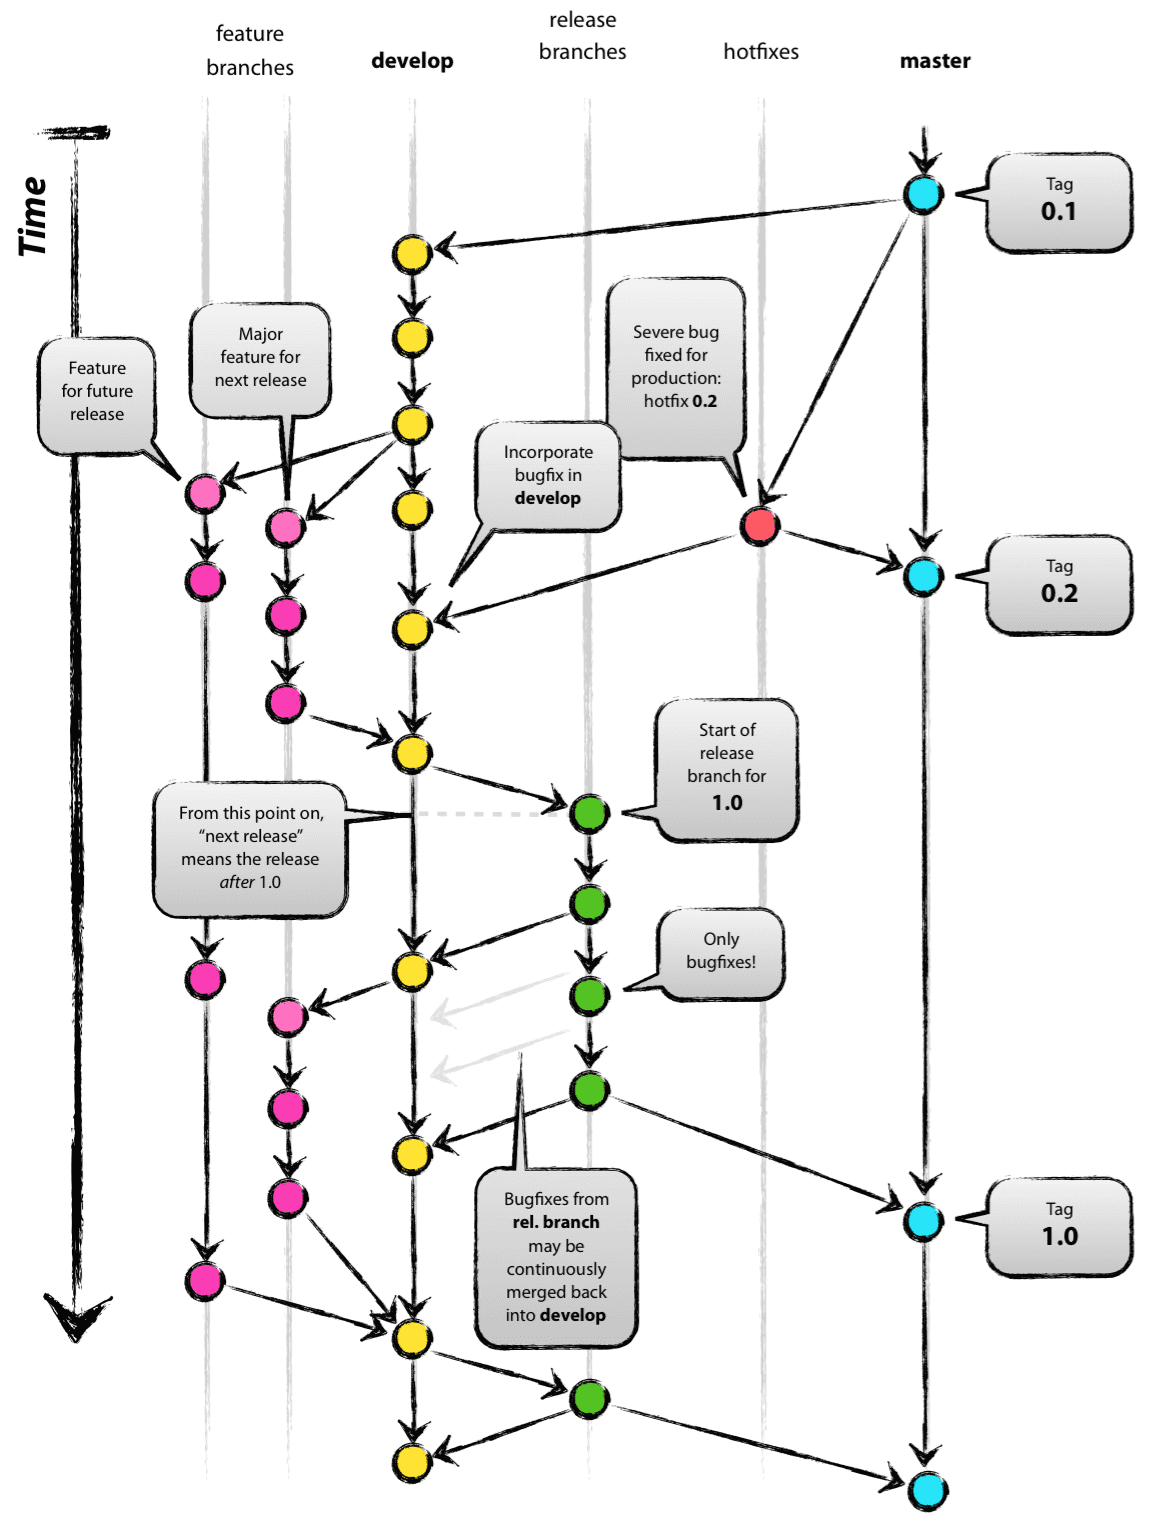
\includegraphics[height=4.5in]{img/git-process.png}
\end{center}
\caption{\small\it Git branching process for master
  and development branches.  New features and ordinary (not hot)
  bugfixes are developed in branches from and merged back into the
  development  branch.  These are then
  collected into releases and merged with the master branch, which
  tracks the releases.  Hotfix branches are like feature or ordinary
  bugfix branches, but branch from master and merge back into master.
  Image courtesy of \citep{Driessen:2010}.}\label{git-process.figure} \end{figure}
%
The basic Git process for branching, releasing, hotfixing, and merging
follows standard Git procedure \citep{Driessen:2010}. A diagram
outlining the process is presented in \reffigure{git-process}. The key
idea is that the master branch is always at the latest release, with
older commits tagged for previous releases.

The development branch always represents the current state of
development. Feature and bugfix branches branch from the development
branch. Before being merged back into the development branch, they
must be wrapped in a pull request for GitHub, which supplies
differences with current code and a forum for code review and comment
on the issue. All branches must have appropriate unit tests and
documentation as part of their pull request before they will be merged
(see \url{https://github.com/stan-dev/stan/wiki/Pull-Request-Template}
for the pull request template which all requests must follow).  Each
pull request must provide a summary of the change, a detailed
description of the intended effect (often coupled with pointers to one
or more issues on the issue tracker and one or more Wiki pages), a
description of how the change was tested and its effects can be
verified, a description of any side effects, a description of any
user-facing documentation changes, and suggestions for reviewers.

Taken together, the testing, code review, and merge process ensures
that the development branch is always in a releasable state.

Git itself provides extensive log facilities for comparing changes
made in any given commit (which has a unique ID under Git) with any
other commit, including the current development or master branch.
GitHub provides further graphical facilities for commentary and
graphical differences.

For each release, the Git logs are scanned and a set of user-facing
release notes provided summarizing the changes. The full set of
changes, including differences with previous versions, is available
through Git.  These logs are complete back to the first version of
Stan, which was originally managed under the Subversion version
control system.

More information on the mechanics of the process are available from
on the Wiki page
\url{https://github.com/stan-dev/stan/wiki/Developer-Process}.

\section{Testing and Validation}

\subsection{Unit Testing}

Stan C++, CmdStan, PyStan, and RStan are all extensively unit tested.
The core C++ code and CmdStan code is tested directly in C++ using the
Google test framework \cite{GoogleTest:2011}. PyStan is tested using
the Python unit testing framework unittest%
%
\footnote{See \url{https://docs.python.org/3/library/unittest.html}.}
%
(formerly called ``PyTest'').  RStan is tested using the RUnit package.%
%
\footnote{See
  \url{http://cran.r-project.org/web/packages/RUnit/index.html}.}

The point of unit testing is to test the program at the application
programmer interface (API) level, not the end-to-end functional level.

The tests are run automatically when pull requests are created through
a continuous integration process. PyStan uses the Travis continuous
integration framework;%
%
\footnote{See \url{https://travis-ci.org} for more on Travis.}
%
Stan C++ and CmdStan use Jenkins.%
%
\footnote{See \url{http://jenkins-ci.org} for more on Jenkins.}
%
The continuous integration servers provide detailed reports of the
various tests they run and whether they succeeded or failed.  If they
failed, console output is available pointing to the failed tests.  The
continuous integration servers also provide graphs and charts
summarizing ongoing and past testing behavior.

Stan and its interfaces' unit tests are all distributed with the
system software and may be run by users on their specific platform
with their specific compilers and configurations to provide support
for the reliability of a particular installation of Stan.

As with any statistical software, users need to be careful to consider
the appropriateness of the statistical model, the ability to fit it
with existing data, and its suitability to its intended application.

The entire source repository is available to users.  A snapshot at any
given release (or commit within a branch) may be downloaded as an
archive (zip file) or may be cloned for development under Git.
Cloning in Git provides a complete copy of all version history,
including every commit to every branch since the beginning of the
project.

User feedback is accommodated through three channels. First, and most
formally, there is an issue tracker for each of Stan C++, CmdStan,
RStan and PyStan, which allows users to submit formal bug reports or
make feature requests.  Any user bug report is reviewed by the
development team, assessed for validity and reproducibility, and
assigned to a specific developer for a particular release target.
A second route for reporting bugs is our users group;  bugs reported
to the user group by users are then submitted to the issue tracker by
the developers and then put through the usual process.  A third method
of bug reporting is informal e-mail or comments; like the user group
reports, these are channeled through the issue tracker by the
developers before being tackled.

Continuous integration is run on a combination of Windows, Mac OS X,
and Linux platforms.  All core Stan C++ code is tested on Windows, Mac
OS, and Linux before release.


\subsection{Functional Testing}

In addition to unit testing at the individual function level, Stan
undergoes rigorous end-to-end testing of its model fitting
functionality. Models with known answers are evaluated for both speed
and accuracy. Models without analytic solutions are evaluated in terms
of MCMC error.


\section{Release Cycles}

At various stages, typically when major new functionality has been
added or a serious bug has been fixed, the development branch is
declared ready for release by the Stan development team. At this
point, the branch is tested one last time on all platforms before
being merged with the master branch. Releases are managed through
GitHub releases mechanism.%
%
\footnote{For example, releases for Stan C++ are available on
\url{https://github.com/stan-dev/stan/releases}.}
%
Each release further bundles the manual and provides both a zipped and
tar-gzipped archive of the release.

Stan is released exclusively as source code, so nothing needs to be
done with respect to binary release management or compatibility.  The
source is tested so that it can be used under Windows, Mac OS X, and
Linux.

Instructions for installing Stan C++, CmdStan, RStan, and PyStan are
managed separately and distributed with the associated product.

\section{Versioning and Release Compatibility}\label{version-numbering.section}

Stan version numbers follow the standard semantic version numbering
pattern in which version numbers are of the form
\code{Major.Minor.Patch}; for example version 2.9.1 is major release
2, minor release 9, and patch release 1.  Semantic versioning signals
important information about features and compatibiltiy for the Stan
language and how it is used.   It does not provide information about
underlying implementation;  changes in implementation do not affect
version numbering in and of itself.

See \refappendix{deprecated-features} for a list of currently
deprecated features and instructions on how to upgrade them.

\subsection{Major Version and Backward Compatiblity}

A change in a library breaks backward compatibility if a program that
worked in the previous version no longer works the same way in the
current version.  For backward-compatibility breaking changes, the
major version number is incremented.  When the major version is
updated, the minor version reverts to 0.  Because breaking backward
compatibility is such a disturbance for users, there are very few
major releases.

\subsection{Minor Version and Forward Compatibility}

A change in a library introduces a new feature if a program that works
in the current version will not work in a previous version; that is,
it breaks forward compatibility.  When a version introduces a new
feature without breaking backward compatibility, its minor version
number is incremented.  Whenever the minor version is incremented, the
patch level reverts to 0.  Most Stan releases increment the minor
version.

\subsection{Bug Fixes and Patch Releases}

If a release does not add new functionality or break backward
compatibility, only its patch version is incremented.  Patch releases
of Stan are made when an important bug is fixed before any new work is
done.  Because Stan keeps its development branch clean, pending
patches are easily rolled into minor releases.

\section{Deprecating and Removing Features}\label{process-deprecation.section}

Before a user-facing feature is removed from software, it is polite to
deprecate it in order to maintain backward compatibility and provide
suggestions for upgrading.  \refappendix{deprecated-features} provides
a description of all of the deprecated features that are still
available in Stan and how to replace them with up-to-date features.

Eventually, deprecated features will be removed (aka retired).  As
explained in \refsection{version-numbering}, removing deprecated
features requires a major version number increment.  Stan 3.0.0 will
retire most if not all of the currently deprecated features.




\section{Availability of Current and Historical Archive Versions}

Current and older versions of Stan C++, CmdStan, RStan, and PyStan are
available through the GitHub pages for the corresponding repository.
Official releases are bundled as archives and available through
GitHub's releases (e.g.,
\url{https://github.com/stan-dev/stan/releases} for Stan C++).

Any intermediate commit is also available through GitHub in one of two
ways. First, all of Stan (or CmdStan, RStan, or PyStan) may be
downloaded by cloning the repository, at which point a user has a
complete record of the entire project's commits and branches. After
first cloning a repository, it may be kept up to date using Git's pull
command (available from the command-line or platform-specific
graphical user interfaces).   An alternative delivery mechanism is as
a zip archive of a snapshot of the system.

\section{Maintenance, Support, and Retirement}

Stan support extends only to the most current release. Specifically,
patches are not backported to older versions.

Early fixes of bugs are available to users in the form of updated
development branches. Snapshots of the entire code base at every
commit, including development patches and official releases, are
available from GitHub.  Git itself may be used to download a complete
clone of the entire source code history at any time.

There is extensive documentation in the form of manuals available for
the Stan language and algorithms
(\url{http://mc-stan.org/users/documentation}), as well as the
interfaces for the command line, R, Python, MATLAB, Mathematica,
Stata, and Julia (\url{http://mc-stan.org/users/interfaces}).

There is also an extensive suite of tutorials and example models
(\url{http://mc-stan.org/users/documentation}) which may be used directly or
modified by users. There is also a fairly extensive set of Wiki pages
geared toward developers
(\url{https://github.com/stan-dev/stan/wiki}).

Issue trackers for reporting bugs and requesting features are
available online for Stan's C++ math library and core library, as well
as for the interfaces (all available from the organization page,
(\url{https://github.com/stan-dev}).

There is Stan forum for both users and developers (see
\url{http://discourse.mc-stan.org}).  The users topics allow users can
request support for installation issues, modeling issues, or
performance/accuracy issues.  These lists all come with built-in
search facilities through their host or simply through top-level
web searches in the search engine of your choice.

A number of books provide introductions to Stan, including {\it
  Bayesian Data Analysis, 3rd Edition} \citep{GelmanEtAl:2013} and
{\it Doing Bayesian Data Analysis, 2nd Edition} \citep{Kruschke:2014}.
All of the examples from two other books have been translated to
Stan, {\it Bayesian Cognitive Modeling: A Practical Course}
\citep{LeeWagenmakers:2013}, {\it The BUGS Book}
\citep{LunnEtAl:2012}, and {\it Data Analysis Using Regression and
  Multilevel-Hierarchical Models} \citep{GelmanHill:2007}.

The major.minor.0 releases are maintained through patch releases
major.minor.$n$ releases.  At each new major.minor.0 release, prior
versions are retired from support.  All efforts are focused on the
current release.  No further development or bug fixes are made
available for earlier versions.  The earlier versions can still be
accessed through version control.


\section{Qualified Personnel}

The members of the Stan development team are drawn from multiple
computational, scientific, and statistical disciplines across
academic, not-for-profit, and industrial laboratories.

Most of Stan's developers have Ph.D. degrees, some have Master's
degrees, and some are currently enrolled as undergraduate or graduate
students. All of the developers with advanced degrees have published
extensively in peer reviewed journals. Several have written books on
statistics and/or computing. Many members of the core development team
were well known internationally outside of their contributions to Stan.
The group overall is widely acknowledged as leading experts in
statistical computing, software development, and applied statistics.

The managers of the development process have extensive industrial
programming experience and have designed or contributed to other
software systems that are still in production.

Institutions at which the members of the Stan development team hold
appointments as of Stan release 2.17.1 include Columbia University,
Adobe Creative Technologies Lab, University of Warwick, University of
Toronto (Scarborough), Dartmouth College, University of Washington,
Lucidworks, CNRS (Paris), St. George's, University of London,
University of Massachussetts (Amherst), Aalto University, and Novartis
Pharma.

\section{Physical and Logical Security}

The Stan project maintains its integration servers for Stan C++ and
CmdStan on site at Columbia University. The integration servers for
Stan C++ and CmdStan are password protected and run on isolated,
standalone machines used only as integration servers. The network is
maintained by Columbia University's Information Technology (CUIT)
group.

The integration server for PyStan is hosted by the Travis open-source
continuous integration project, and is password protected on an
account basis.

The version control system is hosted by GitHub
(\url{http://github.com}). Due to Git's distributed nature, each
developer maintains a complete record of the entire project's commit
history. Everything is openly available, but privileges to modify the
existing branches is restricted to the core developers. Any change to
the code base is easily reversed through Git.

The archived releases as well as clones of the full repositories are
also managed through GitHub.

Stan's web pages are served by Pair, Inc. (\url{http://pair.com}) and
are password protected.  The web pages are purely informational and
nothing is distributed through the web page.

Individual contributors work on their own personal computers or on
compute clusters at Columbia or elsewhere.


\section{Disaster Recovery}

The entire history of the Stan C++, CmdStan, RStan, and PyStan
repositories is maintained on the GitHub servers as well as on each
developer's individual copy of the repository. Specifically, each
repository can be reconstituted from any of the core
developers' machines.


\chapter{Reproducibility}\label{reproducibility.chapter}

\noindent
Floating point operations on modern computers are notoriously
difficult to replicate because the fundamental arithmetic operations,
right down to the IEEE 754 encoding level, are not fully specified.
The primary problem is that the precision of operations varies across
different hardware platforms and software implementations.

Stan is designed to allow full reproducibility.  However, this is only
possible up to the external constraints imposed by floating point
arithmetic.

Stan results will only be exactly reproducible if {\it all}\, of the following
components are {\it identical}\,:
%
\begin{itemize}
\item Stan version
\item Stan interface (RStan, PyStan, CmdStan) and version, plus version
  of interface language (R, Python, shell)
\item versions of included libraries (Boost and Eigen)
\item operating system version
\item computer hardware including CPU, motherboard and memory
\item \Cpp compiler, including version, compiler flags, and linked libraries
\item same configuration of call to Stan, including random seed, chain
  ID, initialization and data
\end{itemize}
%
It doesn't matter if you use a stable release version of Stan or the
version with a particular Git hash tag.  The same goes for all of the
interfaces, compilers, and so on.  The point is that if any of
these moving parts changes in some way, floating point results may
change.

Concretely, if you compile a single Stan program using the same
CmdStan code base, but changed the optimization flag (\code{-O3} vs.\
\code{-O2} or \code{-O0}), the two programs may not return the identical
stream of results.  Thus it is very hard to guarantee reproducibility
on externally managed hardware, like in a cluster or even a desktop
managed by an IT department or with automatic updates turned on.

If, however, you compiled a Stan program today using one set of flags,
took the computer away from the internet and didn't allow it to update
anything, then came back in a decade and recompiled the Stan program
in the same way, you should get the same results.

The data needs to be the same down to the bit level. For example, if
you are running in RStan, Rcpp handles the conversion between R's
floating point numbers and C++ doubles. If Rcpp changes the conversion
process or use different types, the results are not guaranteed to be
the same down to the bit level.

The compiler and compiler settings can also be an issue.  There is a
nice discussion of the issues and how to control reproducibility in
Intel's proprietary compiler by \cite{CordenKreitzer:2014}.



\chapter{Contributed Modules}

\noindent
Stan is an open-source project and welcomes user contributions.

In order to reduce maintenance on the main trunk of Stan development
and to allow developer-specified licenses, contributed Stan modules
are not distributed as part of Stan itself.


\section{Contributing a Stan Module}

Developers who have a Stan module to contribute should contact the
Stan developers either through one of the following.
%
\begin{itemize}
\item Stan forums: \
\\
\url{http://discourse.mc-stan.org}
\item Stan e-mail: \
\\
\href{mailto:mc.stanislaw@gmail.com}{\tt mc.stanislaw@gmail.com}
\end{itemize}


\section{GitHub-Hosted Modules}

The \code{stan-dev} organization on GitHub hosts contributed projects
on GitHub.  This is also where the Stan developers will host works in
progress.  The full list of contributed projects on GitHub for
\code{stan-dev} is available at the following location.
%
\begin{quote}
\url{https://github.com/stan-dev}
\end{quote}

Each contributed module on \code{stan-dev}'s GitHub space comes with
its own documentation, indexed by the \code{README.md} file displayed
on GitHub.  Each contributed module has its own licensing the terms of
which are controlled by its developers.  The license for a contributed
package and its dependencies can be found in a top-level directory
\code{licenses/}.

\subsection{Emacs Stan Mode}

\noindent
Emacs Stan mode allows syntax highlighting and automatic indentation
of Stan models in the Emacs text editor.

\begin{quote}
\begin{tabular}{rl}
{\it Repository:} & \url{https://github.com/stan-dev/stan-mode}
\\[4pt]
{\it License:} & GPLv3
\\[4pt]
{\it Authors:} & Jeffrey Arnold, Daniel Lee
\end{tabular}
\end{quote}

\chapter{Stan Program Style Guide}

\noindent
This chapter describes the preferred style for laying out Stan
models. These are not rules of the language, but simply
recommendations for laying out programs in a text editor.  Although
these recommendations may seem arbitrary, they are similar to those of
many teams for many programming languages.  Like rules for typesetting
text, the goal is to achieve readability without wasting white space
either vertically or horizontally.

\section{Choose a Consistent Style}

The most important point of style is consistency.  Consistent coding
style makes it easier to read not only a single program, but multiple
programs.  So when departing from this style guide, the number one
recommendation is to do so consistently.

\section{Line Length}

Line lengths should not exceed 80 characters.%
%
\footnote{Even 80 characters may be too many for rendering in print;
  for instance, in this manual, the number of code characters that fit
  on a line is about 65.}
%
This is a typical recommendation for many programming language style
guides because it makes it easier to lay out text edit windows side by
side and to view the code on the web without wrapping, easier to view
diffs from version control, etc.  About the only thing that is
sacrificed is laying out expressions on a single line.

\section{File Extensions}

The recommended file extension for Stan model files is \code{.stan}.
For Stan data dump files, the recommended extension is \code{.R}, or
more informatively, \code{.data.R}.

\section{Variable Naming}

The recommended variable naming is to follow C/\Cpp naming
conventions, in which variables are lowercase, with the underscore
character (\Verb|_|) used as a separator.  Thus it is preferred to use
\Verb|sigma_y|, rather than the run together \Verb|sigmay|, camel-case
\Verb|sigmaY|, or capitalized camel-case \Verb|SigmaY|.  Even matrix
variables should be lowercased.

The exception to the lowercasing recommendation, which also follows
the C/\Cpp conventions, is for size constants, for which the
recommended form is a single uppercase letter.  The reason for this is
that it allows the loop variables to match.  So loops over the indices of
an $M \times N$ matrix $a$ would look as follows.
%
\begin{stancode}
for (m in 1:M)
  for (n in 1:N)
     a[m,n] = ...
\end{stancode}


\section{Local Variable Scope}

Declaring local variables in the block in which they are used aids in
understanding programs because it cuts down on the amount of text
scanning or memory required to reunite the declaration and definition.

The following Stan program corresponds to a direct translation of a
BUGS model, which uses a different element of \code{mu} in each
iteration.
%
\begin{stancode}
model {
  real mu[N];
  for (n in 1:N) {
    mu[n] = alpha * x[n] + beta;
    y[n] ~ normal(mu[n],sigma);
  }
}
\end{stancode}
%
Because variables can be reused in Stan and because they should be
declared locally for clarity, this model should be recoded as follows.
%
\begin{stancode}
model {
  for (n in 1:N) {
    real mu;
    mu = alpha * x[n] + beta;
    y[n] ~ normal(mu,sigma);
  }
}
\end{stancode}
%
The local variable can be eliminated altogether, as follows.
%
\begin{stancode}
model {
  for (n in 1:N)
    y[n] ~ normal(alpha * x[n] + beta, sigma);
}
\end{stancode}
%
There is unlikely to be any measurable efficiency difference
between the last two implementations, but both should be a bit
more efficient than the BUGS translation.

\subsubsection{Scope of Compound Structures with Componentwise Assignment}

In the case of local variables for compound structures, such as
arrays, vectors, or matrices, if they are built up component by
component rather than in large chunks, it can be more efficient to
declare a local variable for the structure outside of the block
in which it is used.  This allows it to be allocated once and then
reused.
%
\begin{stancode}
model {
  vector[K] mu;
  for (n in 1:N) {
    for (k in 1:K)
      mu[k] = ...;
    y[n] ~ multi_normal(mu,Sigma);
}
\end{stancode}
%
In this case, the vector \code{mu} will be allocated
outside of both loops, and used a total of \code{N} times.

\section{Parentheses and Brackets}

\subsection{Optional Parentheses for Single-Statement Blocks}

Single-statement blocks can be rendered in one of two ways.  The fully
explicit bracketed way is as follows.
%
\begin{stancode}
for (n in 1:N) {
  y[n] ~ normal(mu,1);
}
\end{stancode}
%
The following statement without brackets has the same effect.
%
\begin{stancode}
for (n in 1:N)
  y[n] ~ normal(mu,1);
\end{stancode}
%
Single-statement blocks can also be written on a single line, as
in the following example.
%
\begin{stancode}
for (n in 1:N) y[n] ~ normal(mu,1);
\end{stancode}
%
These can be much harder to read than the first example. Only use this
style if the statement is very simple, as in this example.  Unless
there are many similar cases, it's almost always clearer to put
each sampling statement on its own line.

Conditional and looping statements may also be written without brackets.

The use of for loops without brackets can be dangerous.  For instance,
consider this program.
%
\begin{stancode}
for (n in 1:N)
  z[n] ~ normal(nu,1);
  y[n] ~ normal(mu,1);
\end{stancode}
%
Because Stan ignores whitespace and the parser completes a statement
as eagerly as possible (just as in C++), the previous program is
equivalent to the following program.
%
\begin{stancode}
for (n in 1:N) {
  z[n] ~ normal(nu,1);
}
y[n] ~ normal(mu,1);
\end{stancode}
%


\subsection{Parentheses in Nested Operator Expressions}

The preferred style for operators minimizes parentheses.  This reduces
clutter in code that can actually make it harder to read expressions.
For example, the expression \code{a~+~b~*~c} is preferred to the
equivalent \code{a~+~(b~*~c)} or \code{(a~+~(b~*~c))}.  The operator
precedences and associativities follow those of pretty much every
programming language including Fortran, C++, R, and Python;  full 
details are provided in the reference manual.

Similarly, comparison operators can usually be written with minimal
bracketing, with the form \code{y[n] > 0 || x[n] != 0} preferred to
the bracketed form \code{(y[n] > 0) || (x[n] != 0)}.

\subsection{No Open Brackets on Own Line}

Vertical space is valuable as it controls how much of a program you
can see.  The preferred Stan style is as shown in the previous
section, not as follows.
%
\begin{stancode}
for (n in 1:N)
{
  y[n] ~ normal(mu,1);
}
\end{stancode}
%
This also goes for parameters blocks, transformed data blocks,
which should look as follows.
%
\begin{stancode}
transformed parameters {
  real sigma;
  ...
}
\end{stancode}
%


\section{Conditionals}

Stan supports the full \Cpp-style conditional syntax,
allowing real or integer values to act as conditions, as follows.
%
\begin{stancode}
real x;
...
if (x) {
   // executes if x not equal to 0
   ...
}
\end{stancode}
%

\subsection{Explicit Comparisons of Non-Boolean Conditions}

The preferred form is to write the condition out explicitly for
integer or real values that are not produced as the result of a
comparison or boolean operation, as follows.
%
\begin{stancode}
if (x != 0) ...
\end{stancode}


\section{Functions}

Functions are laid out the same way as in languages such as Java and
\Cpp.  For example,
%
\begin{stancode}
real foo(real x, real y) {
  return sqrt(x * log(y));
}
\end{stancode}
%
The return type is flush left, the parentheses for the arguments are
adjacent to the arguments and function name, and there is a space
after the comma for arguments after the first.  The open curly brace
for the body is on the same line as the function name, following the
layout of loops and conditionals.  The body itself is indented; here
we use two spaces.  The close curly brace appears on its own line.
%
If function names or argument lists are long, they can be
written as
%
\begin{stancode}
matrix
function_to_do_some_hairy_algebra(matrix thingamabob,
                                  vector doohickey2) {
  ...body...
}
\end{stancode}
%
The function starts a new line, under the type.  The arguments are
aligned under each other.

Function documentation should follow the Javadoc and Doxygen styles.
Here's an example repeated from \refsection{documenting-functions}.
%
\begin{stancode}
/**
 * Return a data matrix of specified size with rows
 * corresponding to items and the first column filled
 * with the value 1 to represent the intercept and the
 * remaining columns randomly filled with unit-normal draws.
 *
 * @param N Number of rows correspond to data items
 * @param K Number of predictors, counting the intercept, per
 *          item.
 * @return Simulated predictor matrix.
 */
matrix predictors_rng(int N, int K) {
  ...
\end{stancode}
%
The open comment is \code{/**}, asterisks are aligned below the first
asterisk of the open comment, and the end comment \code{*/} is also
aligned on the asterisk.  The tags \code{@param} and \code{@return}
are used to label function arguments (i.e., parameters) and return
values.

\section{White Space}

Stan allows spaces between elements of a program.  The white space
characters allowed in Stan programs include the space (ASCII
\code{0x20}), line feed (ASCII \code{0x0A}), carriage return
(\code{0x0D}), and tab (\code{0x09}).  Stan treats all whitespace
characters interchangeably, with any sequence of whitespace characters
being syntactically equivalent to a single space character.
Nevertheless, effective use of whitespace is the key to good program
layout.


\subsection{Line Breaks Between Statements and Declarations}

It is dispreferred to have multiple statements or declarations on the
same line, as in the following example.
%
\begin{stancode}
transformed parameters {
  real mu_centered;  real sigma;
  mu = (mu_raw - mean_mu_raw);    sigma = pow(tau,-2);
}
\end{stancode}
%
These should be broken into four separate lines.

\subsection{No Tabs}

Stan programs should not contain tab characters.  They are legal and
may be used anywhere other whitespace occurs.  Using tabs to layout a
program is highly unportable because the number of spaces
represented by a single tab character varies depending on which
program is doing the rendering and how it is configured.

\subsection{Two-Character Indents}

Stan has standardized on two space characters of indentation, which is
the standard convention for C/C++ code.  Another sensible choice is
four spaces, which is the convention for Java and Python.  Just be
consistent.

\subsection{Space Between \code{if} and Condition}

Use a space after \code{if}s.  For instance, use \code{if (x < y) ...}, not
\code{if(x < y) ...}.

\subsection{No Space For Function Calls}

There is no space between a function name and the function it applies
to.  For instance, use \code{normal(0,1)}, not \code{normal (0,1)}.

\subsection{Spaces Around Operators}

There should be spaces around binary operators.  For instance, use
\code{y[1]~=~x}, not \code{y[1]=x}, use \code{(x~+~y)~*~z} not
\code{(x+y)*z}.

\subsection{Breaking Expressions across Lines}

Sometimes expressions are too long to fit on a single line.  In that
case, the recommended form is to break \emph{before} an operator,%
%
\footnote{This is the usual convention in both typesetting and other
  programming languages. Neither R nor BUGS allows breaks before an
  operator because they allow newlines to signal the end of an
  expression or statement.}
%
aligning the operator to indicate scoping.  For example, use the
following form (though not the content; inverting matrices is almost
always a bad idea).
%
\begin{stancode}
target += (y - mu)' * inv(Sigma) * (y - mu);
\end{stancode}
%
Here, the multiplication operator (\code{*}) is aligned to clearly
signal the multiplicands in the product.

For function arguments, break after a comma and line the next
argument up underneath as follows.
%
\begin{stancode}
y[n] ~ normal(alpha + beta * x + gamma * y,
              pow(tau,-0.5));
\end{stancode}
%

\subsection{Optional Spaces after Commas}

Optionally use spaces after commas in function arguments for clarity.
For example, \code{normal(alpha * x[n] + beta,sigma)} can also be
written as \code{normal(alpha~*~x[n]~+~beta,~sigma)}.



\subsection{Unix Newlines}

Wherever possible, Stan programs should use a single line feed
character to separate lines.  All of the Stan developers (so far, at
least) work on Unix-like operating systems and using a standard
newline makes the programs easier for us to read and share.

\subsubsection{Platform Specificity of Newlines}

Newlines are signaled in Unix-like operating systems such as Linux and
Mac OS X with a single line-feed (LF) character (ASCII code point
\code{0x0A}).  Newlines are signaled in Windows using two characters,
a carriage return (CR) character (ASCII code point \code{0x0D})
followed by a line-feed (LF) character.


\appendix
\part*{Appendices}
\addcontentsline{toc}{part}{Appendices}


\chapter{Licensing}\label{licensing.appendix}

\noindent
Stan and its two dependent libraries, Boost and Eigen, are
distributed under liberal freedom-respecting%
%
\footnote{The link
  \url{http://www.gnu.org/philosophy/open-source-misses-the-point.html}
  leads to a discussion about terms ``open
  source'' and ``freedom respecting.''}
%
licenses approved by the Open Source Initiative.%
\footnote{See \url{http://opensource.org}.}

In particular, the licenses for Stan and its dependent libraries have
no ``copyleft'' provisions requiring applications of Stan to be
open source if they are redistributed.

This chapter describes the licenses for the tools that are distributed
with Stan.  The next chapter explains some of the build tools that
are not distributed with Stan, but are required to build and run
Stan models.

\section{Stan's License}

Stan is distributed under the BSD 3-clause license (BSD New).
%
\begin{quote}
\url{http://www.opensource.org/licenses/BSD-3-Clause}
\end{quote}
%
The copyright holder of each contribution is the developer or his or
her assignee.%
%
\footnote{Universities or companies often own the copyright of
  computer programs developed by their employees.}


\section{Boost License}

Stan uses the Boost library for template metaprograms, traits
programs, the parser, and various numerical libraries for special
functions, probability functions, and random number generators.  Boost
is distributed under the Boost Software License version 1.0.
%
\begin{quote}
\url{http://www.opensource.org/licenses/BSL-1.0}
\end{quote}
%
The copyright for each Boost package is held by its developers or their
assignees.


\section{Eigen License}

Stan uses the Eigen library for matrix arithmetic and linear algebra.
Eigen is distributed under the Mozilla Public License, version 2.
%
\begin{quote}
\url{http://opensource.org/licenses/mpl-2.0}
\end{quote}
%
The copyright of Eigen is owned jointly by its developers or their
assignees.

\section{SUNDIALS License}

Stan uses the SUNDIALS package for solving stiff differential
equations.  SUNDIALS is distributed under the new BSD (3-clause) license.
%
\begin{quote}
\url{https://opensource.org/licenses/BSD-3-Clause}
\end{quote}
%
The copyright of SUNDIALS is owned by Lawrence Livermore National
Security.

\section{Google Test License}

Stan uses Google Test for unit testing; it is not required to compile
or execute models.  Google Test is distributed under the new BSD (3-clause)
license.
%
\begin{quote}
\url{https://opensource.org/licenses/BSD-3-Clause}
\end{quote}
%
The copyright of Google Test is owned by Google, Inc.


\chapter{Stan for Users of BUGS}\label{stan-for-bugs.appendix}

From the outside, Stan and BUGS%
%
\footnote{Except where otherwise noted, we use ``BUGS'' to refer to
  WinBUGS, OpenBUGS, and JAGS, indiscriminately.}
%
are similar --- they use statistically-themed modeling languages
(which are similar but with some differences; see below), they can be
called from R, running some specified number of chains to some
specified length, producing posterior simulations that can be assessed
using standard convergence diagnostics.  This is not a coincidence:
in designing Stan, we wanted to keep many of the useful features of
Bugs.

To start, take a look at the files of translated \BUGS models at
\url{http://mc-stan.org}.  These are 40 or so models from the \BUGS
example volumes, all translated and tested (to provide the same
answers as \BUGS) in Stan.  For any particular model you want to fit,
you can look for similar structures in these examples.

\section{Some Differences in How BUGS and Stan Work}

\begin{itemize}
\item \BUGS is interpreted; Stan is compiled in two steps, first a
  model is is translated to templated C++ and then to a
  platform-specific executable.  Stan, unlike \BUGS, allows the user
  to directly program in C++, but we do not describe how to do this in
  this Stan manual (see the getting started with \Cpp section of
  \url{http://mc-stan.org} for more information on using Stan directly
  from \Cpp).
\item \BUGS performs \MCMC updating one scalar parameter at a time
  (with some exceptions such as \JAGS's implementation of regression
  and generalized linear models and some conjugate multivariate
  parameters), using conditional distributions (Gibbs sampling) where
  possible and otherwise using adaptive rejection sampling, slice
  sampling, and Metropolis jumping.  \BUGS figures out the dependence
  structure of the joint distribution as specified in its modeling
  language and uses this information to compute only what it needs at
  each step.  Stan moves in the entire space of all the parameters
  using Hamiltonian Monte Carlo (more precisely, the no-U-turn
  sampler), thus avoiding some difficulties that occur with
  one-dimension-at-a-time sampling in high dimensions but at the cost
  of requiring the computation of the entire log density at each step.
\item \BUGS tunes its adaptive jumping (if necessary) during its
  warmup phase (traditionally referred to as "burn-in").  Stan uses
  its warmup phase to tune the no-U-turn sampler (\NUTS).
\item The \BUGS modeling language is not directly executable.  Rather,
  \BUGS parses its model to determine the posterior density and then
  decides on a sampling scheme.  In contrast, the statements in a Stan
  model are directly executable: they translate exactly into C++ code
  that is used to compute the log posterior density (which in turn is
  used to compute the gradient).
\item In \BUGS, the order in which statements are written does not
  matter.  They are executed according to the directed graphical model
  so that variables are always defined when needed.  A side effect of
  the direct execution of Stan's modeling language is that statements
  execute in the order in which they are written.  For instance, the
  following Stan program, which sets \code{mu} before using it to
  sample \code{y}.
%
\begin{stancode}
mu = a + b * x;
y ~ normal(mu,sigma);
\end{stancode}
%
It translates to the following \Cpp code.
%
\begin{stancode}
mu = a + b * x;
lp += normal_log(mu,sigma);
\end{stancode}
%
Contrast this with the Stan program
%
\begin{stancode}
y ~ normal(mu,sigma)
mu = a + b * x
\end{stancode}
%
This program is well formed, but is almost certainly
a coding error, because it attempts to use \code{mu} before
it is set. It translates to the following \Cpp code.
%
\begin{stancode}
lp += normal_log(mu,sigma);
mu = a + b * x;
\end{stancode}
%
The direct translation to the imperative language of \Cpp code
highlights the potential error of using \code{mu} in the first
statement.
\\[8pt]
To trap these kinds of errors, variables are initialized to the
special not-a-number (\code{NaN}) value.  If \code{NaN} is passed to a
log probability function, it will raise a domain exception, which will
in turn be reported by the sampler.  The sampler will reject the
sample out of hand as if it had zero probability.
%
\item Stan uses its own \Cpp algorithmic differentiation packages to
  compute the gradient of the log density (up to a proportion).
  Gradients are required during the Hamiltonian dynamics simulations
  within the leapfrog algorithm of the Hamiltonian Monte Carlo and
  \NUTS samplers.  \BUGS computes the log density but not its
  gradient.
\item Both \BUGS and Stan are semi-automatic in that they run by
  themselves with no outside tuning required. Nevertheless, the user
  needs to pick the number of chains and number of iterations per
  chain.  We usually pick 4 chains and start with 10 iterations per
  chain (to make sure there are no major bugs and to approximately
  check the timing), then go to 100, 1000, or more iterations as
  necessary.  Compared to Gibbs or Metropolis, Hamiltonian Monte Carlo
  can take longer per iteration (as it typically takes many "leapfrog
  steps" within each iteration), but the iterations typically have lower
  autocorrelation.  So Stan might work fine with 1000 iterations in an
  example where \BUGS would require 100,000 for good mixing.  We
  recommend monitoring potential scale reduction statistics ($\hat{R}$)
  and the effective sample size to judge when to stop (stopping when
  $\hat{R}$ values do not counter-indicate convergence and when enough
  effective samples have been collected).
\item WinBUGS is closed source.  OpenBUGS and JAGS are both licensed
  under the Gnu Public License (GPL), otherwise known as copyleft due
  to the restrictions it places on derivative works.  Stan is licensed
  under the much more liberal new BSD license.
\item Like WinBUGS, OpenBUGS and JAGS, Stan can be run directly from
  the command line or through R (Python and MATLAB interfaces are in
  the works)
\item Like OpenBUGS and JAGS, Stan can be run on Linux, Mac, and
  Windows platforms.
\end{itemize}

\section{Some Differences in the Modeling Languages}

\begin{itemize}
\item The \BUGS modeling language follows an R-like syntax in which
  line breaks are meaningful.  Stan follows the rules of C, in which
  line breaks are equivalent to spaces, and each statement ends in a
  semicolon.  For example:
%
\begin{stancode}
y ~ normal(mu, sigma);
\end{stancode}
%
and
%
\begin{stancode}
for (i in 1:n) y[i] ~ normal(mu, sigma);
\end{stancode}
%
Or, equivalently (recall that a line break is just another form of whitespace),
%
\begin{stancode}
for (i in 1:n)
  y[i] ~ normal(mu, sigma);
\end{stancode}
%
and also equivalently,
%
\begin{stancode}
for (i in 1:n) {
  y[i] ~ normal(mu, sigma);
}
\end{stancode}
%
There's a semicolon after the model statement but not after the
brackets indicating the body of the for loop.
%
\item Another C thing: In Stan, variables can have names constructed
  using letters, numbers, and the underscore (\code{\_}) symbol, but
  nothing else (and a variable name cannot begin with a number).
  \BUGS variables can also include the dot, or period (\code{.}) symbol.
%
\item In Stan, the second argument to the "normal" function is the
  standard deviation (i.e., the scale), not the variance (as in {\it
    Bayesian Data Analysis}) and not the inverse-variance (i.e.,
  precision) (as in \BUGS).  Thus a normal with mean 1 and standard
  deviation 2 is \code{normal(1,2)}, not \code{normal(1,4)} or
  \code{normal(1,0.25)}.
%
\item Similarly, the second argument to the "multivariate normal"
  function is the covariance matrix and not the inverse covariance matrix
  (i.e., the precision matrix) (as in \BUGS). The same is true for
  the "multivariate student" distribution.
%
\item
The distributions have slightly different names:
%
\begin{quote}
\begin{tabular}{l|l}
{\it BUGS} & {\it Stan} \\ \hline \hline
\code{dnorm} & \code{normal} \\
\code{dbinom} & \code{binomial} \\
\code{dpois} & \code{poisson} \\
$\vdots$ & $\vdots$
\end{tabular}
\end{quote}
%
\item Stan, unlike \BUGS, allows intermediate quantities, in the form
  of local variables, to be reassigned.  For example, the following is
  legal and meaningful (if possibly inefficient) Stan code.
%
\begin{stancode}
{
  total = 0;
  for (i in 1:n){
    theta[i] ~ normal(total, sigma);
    total = total + theta[i];
  }
}
\end{stancode}
%
In \BUGS, the above model would not be legal because the variable
\code{total} is defined more than once.  But in Stan, the loop is
executed in order, so \code{total} is overwritten in each step.
%
\item Stan uses explicit declarations.  Variables are declared with
  base type integer or real, and vectors, matrices, and arrays have
  specified dimensions.  When variables are bounded, we give that
  information also.  For data and transformed parameters, the bounds
  are used for error checking.  For parameters, the constraints
  are critical to sampling as they determine the geometry over which
  the Hamiltonian is simulated.
  \\[6pt]
  Variables can be declared as data, transformed data, parameters, transformed
  parameters, or generated quantities.  They can also be declared as
  local variables within blocks.  For more information, see
  the part of this manual devoted to the Stan programming language and
  examine at the example models.
%
\item Stan allows all sorts of tricks with vector and matrix
  operations which can make Stan models more compact.  For example,
  arguments to probability functions may be vectorized,%
%
\footnote{Most distributions have been vectorized, but currently the
truncated versions may not exist and may not be vectorized.}
%
allowing
%
\begin{stancode}
for (i in 1:n)
  y[i] ~ normal(mu[i], sigma[i]);
\end{stancode}
%
to be expressed more compactly as
%
\begin{stancode}
y ~ normal(mu,sigma);
\end{stancode}
%
The vectorized form is also more efficient because Stan can unfold the
computation of the chain rule during algorithmic differentiation.
%
\item Stan also allows for arrays of vectors and matrices.
  For example, in a hierarchical model might have a vector of \code{K}
  parameters for each of \code{J} groups; this can be declared using
\begin{stancode}
vector[K] theta[J];
\end{stancode}
%
Then \code{theta[j]} is an expression denoting a \code{K}-vector and
may be used in the code just like any other vector variable.
\\[6pt]
An alternative encoding would be with a two-dimensional array, as in
\begin{stancode}
real theta[J,K];
\end{stancode}
%
The vector version can have some advantages, both in convenience and
in computational speed for some operations.
\\[6pt]
A third encoding would use a matrix:
%
\begin{stancode}
matrix[J,K] theta;
\end{stancode}
%
but in this case, \code{theta[j]} is a row vector, not a vector, and
accessing it as a vector is less efficient than with an array of
vectors.  The transposition operator, as in \code{theta[j]'}, may be
used to convert the row vector \code{theta[j]} to a (column) vector.
Column vector and row vector types are not interchangeable everywhere
in Stan; see the function signature declarations in the programming
language section of this manual.
%
\item Stan supports general conditional statements using a standard
  if-else syntax.  For example, a zero-inflated (or -deflated) Poisson
  mixture model is defined using the if-else syntax as described in
  \refsection{zero-inflated}.
%
\item Stan supports general while loops using a standard syntax.
While loops give Stan full Turing equivalent computational power.
They are useful for defining iterative functions with complex
termination conditions.  As an illustration of their syntax,
the for-loop
%
\begin{stancode}
model {
    ....
    for (n in 1:N) {
        ... do something with n ....
    }
}
\end{stancode}
%
may be recoded using the following while loop.
%
\begin{stancode}
model {
    int n;
    ...
    n = 1;
    while (n <= N) {
        ... do something with n ...
        n = n + 1;
    }
}
\end{stancode}
%


\end{itemize}


\section{Some Differences in the Statistical Models that are Allowed}

\begin{itemize}
\item Stan does not yet support estimation of discrete parameters
  (discrete data is supported).  We may eventually implement a
  combination of Gibbs and slice sampling for discrete parameters, but
  we haven't done so yet.
\item Stan has some distributions on covariance matrices that do not
  exist in \BUGS, including a uniform distribution over correlation
  matrices which may be rescaled, and the priors based on C-vines
  defined in \citep{LewandowskiKurowickaJoe:2009}.  In particular, the
  Lewandowski et al.\ prior allows the correlation matrix to be shrunk
  toward the unit matrix while the scales are given independent priors.
\item In \BUGS you need to define all variables.  In Stan, if you
  declare but don't define a parameter it implicitly has a flat prior
  (on the scale in which the parameter is defined).  For example, if
  you have a parameter \code{p} declared as
\begin{stancode}
real<lower=0,upper=1> p;
\end{stancode}
%
and then have no sampling statement for \code{p} in the \code{model}
block, then you are implicitly assigning a uniform $[0,1]$ prior on
\code{p}.
On the other hand, if you have a parameter \code{theta} declared with
%
\begin{stancode}
real theta;
\end{stancode}
%
and have no sampling statement for \code{theta} in the
\code{model} block,
 then you are implicitly assigning an improper uniform prior
on $(-\infty,\infty)$ to \code{theta}.
%
% Then if
% you define a transformed parameter \code{p} using
% \begin{stancode}
% p = invlogit(theta);
% \end{stancode}
% %
% then you get a $\distro{Beta}(0,0)$ on \code{p}.
% then you are implicitly assigning an improper uniform
% (-infinity, infinity) prior on theta, which corresponds to a Beta
% (0,0) prior on p.  You could also assign this latter prior directly by
% defining p as the parameter and then writing the following within the
% model: p ~ beta (0, 0);
\item \BUGS models are always proper (being constructed as a product
  of proper marginal and conditional densities).  Stan models can be
  improper.  Here is the simplest improper Stan model:
\begin{stancode}
parameters {
  real theta;
}
model { }
\end{stancode}
% \item You can also define some improper models in \BUGS directly, for
%   example, \Verb|p ~ beta (0, 0);| Remember how Stan works:
%   lines in the model are executables that correspond directly to
%   factors in the posterior density.  So you can define beta(0,0), it's
%   simply a mathematical function.  Stan doesn't "care" if it has a
%   finite integral.
\item Although parameters in Stan models may have improper priors, we
  do not want improper \emph{posterior} distributions, as we are trying to
  use these distributions for Bayesian inference.  There is no general
  way to check if a posterior distribution is improper.  But if all
  the priors are proper, the posterior will be proper also.
\item
  As noted earlier, each statement in a Stan model is directly translated into the \Cpp code for computing the log posterior.  Thus, for example, the following pair of statements is legal in a Stan model:
\begin{stancode}
y ~ normal(0,1);
y ~ normal(2,3);
\end{stancode}
%
The second line here does \emph{not} simply overwrite the first;
rather, \emph{both} statements contribute to the density function that
is evaluated.  The above two lines have the effect of including the
product, $\distro{Norm}(y|0,1) \times \distro{Norm}(y|2,3)$, into the
density function.
\\[6pt]
For a perhaps more confusing example, consider the following two lines in a Stan model:
\begin{stancode}
x ~ normal(0.8*y, sigma);
y ~ normal(0.8*x, sigma);
\end{stancode}
%
At first, this might look like a joint normal distribution with a
correlation of 0.8.  But it is not.  The above are \emph{not}
interpreted as conditional entities; rather, they are factors in the
joint density.  Multiplying them gives, $\distro{Norm}(x|0.8y,\sigma)
\times \distro{Norm}(y|0.8x,\sigma)$, which is what it is (you can
work out the algebra) but it is not the joint distribution where the
conditionals have regressions with slope 0.8.
%
\item With censoring and truncation, Stan uses the censored-data or
  truncated-data likelihood---this is not always done in \BUGS.  All
  of the approaches to censoring and truncation discussed in
  \citep{GelmanEtAl:2013} and \citep{GelmanHill:2007} may
  be implemented in Stan directly as written.
%
\item Stan, like \BUGS, can benefit from human intervention in the
  form of reparameterization.  More on this topic to come.
  % For example, with the 8 schools: . . .
\end{itemize}

\section{Some Differences when Running from R}

\begin{itemize}

\item Stan can be set up from within R using two lines of code.
  Follow the instructions for running Stan from R on
  \url{http://mc-stan.org}.  You don't need to separately download
  Stan and RStan.  Installing RStan will automatically set up Stan.
  When RStan moves to CRAN, it will get even easier.
\item In practice we typically run the same Stan model repeatedly.  If
  you pass RStan the result of a previously fitted model the model will
  not need be recompiled. An example is given on the running
  Stan from R pages available from \code{http://mc-stan.org}.
\item When you run Stan, it saves various conditions including
  starting values, some control variables for the tuning and running
  of the no-U-turn sampler, and the initial random seed. You can
  specify these values in the Stan call and thus achieve exact
  replication if desired.  (This can be useful for debugging.)
\item When running \BUGS from R, you need to send exactly the data
  that the model needs.  When running RStan, you can include extra
  data, which can be helpful when playing around with models.  For
  example, if you remove a variable \code{x} from the model, you can keep
  it in the data sent from R, thus allowing you to quickly alter the
  Stan model without having to also change the calling information in
  your R script.
\item As in R2WinBUGS and R2jags, after running the Stan model, you
  can quickly summarize using \code{plot()} and \code{print()}.  You
  can access the simulations themselves using various extractor
  functions, as described in the RStan documentation.
\item Various information about the sampler, such as number of
  leapfrog steps, log probability, and step size, is available through
  extractor functions.   These can be useful for understanding what is
  going wrong when the algorithm is slow to converge.
\end{itemize}

\section{The Stan Community}

\begin{itemize}
\item Stan, like WinBUGS, OpenBUGS, and JAGS, has an active community,
  which you can access via the user's mailing list and the developer's
  mailing list; see \code{http://mc-stan.org} for information on
  subscribing and posting and to look at archives.
\end{itemize}

\chapter{Modeling Language Syntax}

\noindent
This chapter defines the basic syntax of the Stan modeling language
using a Backus-Naur form (\BNF) grammar plus extra-grammatical
constraints on function typing and operator precedence and
associativity.

\section{BNF Grammars}

\subsection{Syntactic Conventions}

In the following \BNF grammars, literal strings are indicated in
single quotes (\Verb|'|).  Grammar non-terminals are unquoted strings.
A prefix question mark (\code{?A}) indicates optionality of \code{A}.
A postfixed Kleene star (\code{A*}) indicates zero or more occurrences
of \code{A}.  The notation \code{A \% B}, following the Boost Spirit
parser library's notation, is shorthand for \code{?(A (B A)*)}, i.e.,
any number of \code{A} (including zero), separated by \code{B}.  A
postfixed, curly-braced number indicates a fixed number of repetitions;
e.g., \code{A\{6\}} is equivalent to a sequence of six copies of \code{A}.

\subsection{Programs}

{\small
\begin{Verbatim}
program ::= ?functions ?data ?tdata ?params ?tparams model ?generated

functions ::= 'functions' function_decls
data ::= 'data' var_decls
tdata ::= 'transformed data' var_decls_statements
params ::= 'parameters' var_decls
tparams ::= 'transformed parameters' var_decls_statements
model ::= 'model' statement
generated ::= 'generated quantities' var_decls_statements

function_decls ::= '{' function_decl* '}'
var_decls ::= '{' var_decl* '}'
var_decls_statements ::= '{' var_decl* statement* '}'
\end{Verbatim}
}

\subsection{Function Declarations}

{
\small
\begin{Verbatim}[fontsize=\small]
function_decl ::= unsized_return_type identifier '(' unsized_types ')'
                 statement

unsized_return_type ::= 'void' | unsized_type
unsized_type ::= (basic_type ?unsized_dims)
unsized_types ::= unsized_type % ','
basic_type ::= 'int' | 'real' | 'vector' | 'row_vector' | 'matrix'
unsized_dims ::= '['  ','*  ']'
\end{Verbatim}
}

\subsection{Variable Declarations}

{
\small
\begin{Verbatim}[fontsize=\small]
var_decl ::= var_type variable ?dims ?('=' expression) ';'

var_type ::= 'int' range_constraint
           | 'real' range_constraint
           | 'vector' range_constraint '[' expression ']'
           | 'ordered' '[' expression ']'
           | 'positive_ordered' '[' expression ']'
           | 'simplex' '[' expression ']'
           | 'unit_vector' '[' expression ']'
           | 'row_vector' range_constraint '[' expression ']'
           | 'matrix' range_constraint '[' expression ',' expression ']'
           | 'cholesky_factor_corr' '[' expression ']'
           | 'cholesky_factor_cov' '[' expression ?(',' expression) ']'
           | 'corr_matrix' '[' expression ']'
           | 'cov_matrix' '[' expression ']'

range_constraint ::= ?('<' range '>')

range ::= 'lower' '=' expression ',' 'upper' = expression
        | 'lower' '=' expression
        | 'upper' '=' expression

dims ::= '['  expressions ']'

variable ::= identifier

identifier ::= [a-zA-Z] [a-zA-Z0-9_]*
\end{Verbatim}
}

\subsection{Expressions}

{
\small
\begin{Verbatim}[fontsize=\small]
expressions ::= expression % ','
expression ::= real_literal
             | variable
             | '{' expressions '}'
             | expression `?` expression `:` expression
             | expression infixOp expression
             | prefixOp expression
             | expression postfixOp
             | expression '[' indexes ']'
             | function_literal '(' ?expressions ')'
             | function_literal '(' expression ?('|' expression % ',') ')'
             | integrate_ode '(' function_literal (',' expression){6} ')'
             | integrate_ode_rk45
               '(' function_literal (',' expression){6|9} ')'
             | integrate_ode_bdf
               '(' function_literal (',' expression){6|9} ')'
             | algebra_solver
             '('function_literal (',' expression){4|7} ')'
             | '(' expression ')'

index ::= ?(expression | expression ':' | ':' expression
            | expression ':' expression)

indexes ::= index % ','

integer_literal ::= 0 | [1-9] [0-9]*

real_literal ::= integer_literal ?('.' [0-9]*) ?exp_literal

exp_literal ::= ('e' | 'E') integer_literal

function_literal ::= identifier
\end{Verbatim}
}

\subsection{Statements}

{
\small
\begin{Verbatim}[fontsize=\small]
statement ::= atomic_statement | nested_statement

atomic_statement ::= atomic_statement_body ';'
atomic_statement_body
::=  lhs assignment_op expression
   | expression '~' identifier '(' expressions ')' ?truncation
   | function_literal '(' expressions ')'
   | 'increment_log_prob' '(' expression ')'
   | 'target' '+=' expression
   | 'break'
   | 'continue'
   | 'print' '(' (expression | string_literal) % ',' ')'
   | 'reject' '(' (expression | string_literal) % ',' ')'
   | 'return' expression
   | ''

assignment_op ::= '<-' | '=' | '+=' | '-=' | '*=' | '/=' | '.*=' | '/*='

string_literal ::= '"' char* '"'

truncation ::= 'T' '[' ?expression ',' ?expression ']'

lhs ::= identifier ?('[' indexes ']')

nested_statement
::=
  | 'if' '(' expression ')' statement
    ('else' 'if' '(' expression ')' statement)*
    ?('else' statement)
  | 'while' '(' expression ')' statement
  | 'for' '(' identifier 'in' expression ':' expression ')' statement
  | 'for' '(' identifier 'in' expression ')' statement
  | '{' var_decl* statement+ '}'
\end{Verbatim}
%
}

\section{Extra-Grammatical Constraints}

\subsection{Type Constraints}

A well-formed Stan program must satisfy the type constraints imposed
by functions and distributions.  For example, the binomial
distribution requires an integer total count parameter and integer
variate and when truncated would require integer truncation points.
If these constraints are violated, the program will be rejected during
parsing with an error message indicating the location of the problem.
For information on argument types, see \refpart{built-in-functions}.

\subsection{Operator Precedence and Associativity}

In the Stan grammar provided in this chapter, the expression \code{1
  + 2 * 3} has two parses.  As described in
\refsection{arithmetic-expressions}, Stan disambiguates between the
meaning $1 + (2 \times 3)$ and the meaning $(1 + 2) \times 3$ based on
operator precedences and associativities.

\subsection{Typing of Compound Declaration and Definition}

In a compound variable declaration and definition, the type of the
right-hand side expression must be assignable to the variable being
declared.  The assignability constraint restricts compound
declarations and definitions to local variables and variables declared
in the transformed data, transformed parameters, and generated
quantities blocks.

\subsection{Typing of Array Expressions}

The types of expressions used for elements in array expressions
(\Verb|'{' expressions '}'|) must all be of the same type or a mixture
of \code{int} and \code{real} types (in which case the result is
promoted to be of type \code{real}).

\subsection{Forms of Numbers}

Integer literals longer than one digit may not start with 0 and real
literals cannot consist of only a period or only an exponent.

\subsection{Conditional Arguments}

Both the conditional if-then-else statement and while-loop statement
require the expression denoting the condition to be a primitive type,
integer or real.

\subsection{For Loop Containers}

The for loop statement requires that we specify in addition to the
loop identifier, either a range consisting of two expressions
denoting an integer, separated by ':', or a single expression denoting
a container.

\subsection{Print Arguments}

The arguments to a print statement cannot be void.

\subsection{Only Break and Continue in Loops}

The \code{break} and \code{continue} statements may only be used
within the body of a for-loop or while-loop.

\subsection{PRNG Function Locations}

Functions ending in \code{\_rng} may only be called in the transformed
data and generated quantities block, and within the bodies of
user-defined functions with names ending in \code{\_rng}.

\subsection{Probability Function Naming}

A probability function literal must have one of the following
suffixes: \code{\_lpdf}, \code{\_lpmf}, \code{\_lcdf}, or \code{\_lccdf}.

\subsection{Algebraic Solver Argument Types and Origins}

The \code{algebra\_solver} function may be used without control
parameters; in this case
%
\begin{itemize}
\item its first argument refers to a function with signature
\begin{quote}
  \code{(~vector, ~vector,~real[],~int[])~:~vector},
\end{quote}
\item the remaining four arguments must be assignable to types
\begin{quote}
  \code{vector}, \code{vector}, \code{real[]}, \code{int[]}
\end{quote}
  respectively and
  \item the second, fourth, and fifth arguments must be expressions
  containing only variables originating from the data or transformed
  data blocks.
\end{itemize}
%
The \code{algebra\_solver} function may accept three additional arguments,
which like the second, fourth, and fifth arguments, must be expressions free
of parameter references. The final free arguments must be assignable to types
\begin{quote}
\code{real}, \code{real}, \code{int}
\end{quote}


\subsection{ODE Solver Argument Types and Origins}

The \code{integrate\_ode}, \code{integrate\_ode\_rk45}, and
\code{integrate\_ode\_bdf} functions may be used without control
parameters;  in this case
%
\begin{itemize}
\item its first argument to refer to a function with signature
\begin{quote}
 \code{(real,~real[],~real[],~real[],~int[])~:~real[]},
\end{quote}
\item the remaining six arguments must assignable to types
\begin{quote}
  \code{real[]}, \code{real}, \code{real[]}, \code{real[]},
\code{real[]}, and \code{int[]}
\end{quote}
 respectively, and
\item the third, fourth, and sixth arguments must be expressions not
  containing any variables not originating in the data or transformed
  data blocks.
\end{itemize}
%
The \code{integrate\_ode\_rk45} and \code{integrate\_ode\_bdf}
functions may accept three additional arguments, which like the third,
fourth, and sixth arguments, must be expressions free of parameter
references.  The final three arguments must be assignable to types
\begin{quote}
\code{real}, \code{real}, \code{int}.
\end{quote}

\subsection{Indexes}

Standalone expressions used as indexes must denote either an integer
(\code{int}) or an integer array (\code{int[]}).  Expressions
participating in range indexes (e.g., \code{a} and \code{b} in
\code{a~:~b}) must denote integers (\code{int}).

A second condition is that there not be more indexes provided than
dimensions of the underlying expression (in general) or variable (on
the left side of assignments) being indexed.  A vector or row vector
adds 1 to the array dimension and a matrix adds 2.  That is, the type
\code{matrix[\,,\,,\,]}, a three-dimensional array of matrices, has five
index positions: three for the array, one for the row of the matrix
and one for the column.

\chapter{Warning and Error Messages}\label{error-messages.appendix}

\noindent
This appendix details the specific error messages returned by the
underlying Stan engine.  The individual Stan interfaces (RStan,
PyStan, CmdStan) also return error or warning messages in some
circumstances.

\section{Warnings vs.\ Errors}

The messages returned by Stan come in two flavors, warnings and
errors.  Error messages arise when a fatal problem occurs under the
hood from which there is no way to recover.  Warning messages arise
in circumstances from which the underlying program can continue to
operate.

An example warning message is an informational message about
ill-formed input to an underlying function, which results in a
Metropolis rejection during sampling or a reduction in step size for
optimization, without causing a fatal error.  An example error message
is when either sampling or optimization cannot find a region of
non-zero probability or when a program being parsed is ill formed.
When an error arises, whatever program is running cannot continue and
the entire execution must halt.

\section{Parsing and Compilation}

Both warning messages and error messages may arise during parsing.  If
a Stan program parses successfully, it should compile in \Cpp as
well.  If it does not compile, there is an underlying bug in Stan's
parser and \Cpp code generator.

\begin{itemize}
\item {\it Jacobian may be necessary.}  This message arises when the
  parser cannot verify that the left-hand side of a sampling statement
  is a linear function of a parameter.  If it is not a linear function
  of the parameters, a Jacobian adjustment must be applied.  See
  \refchapter{change-of-variables} for more information on how to
  adjust for the Jacobian of a non-linear transform
\end{itemize}


\section{Initialization}

\begin{itemize}
\item {\it vanishing density.} This message arises when there is a
  problem with initialization not providing a finite log probability.
%
\end{itemize}

\section{Function Evaluation}

\begin{itemize}
\item {\it informational message.}  This message shows up during
  sampling when there is a rejected sample due to an underlying issue
  with input to an underlying function (including probably functions
  and sampling statements).  This is a {\it warning}\, message, not an
  error message.  If it only appears at the beginning of warmup in
  MCMC or during early iterations of optimization, it indicates that
  adaptation has not yet found appropriate scales for the parameters
  and an appropriate overall stepsize.  This causes problem like
  overflow or underflow and thus causes illegal inputs to be passed to
  functions.  Even if this message persists during sampling, the
  Metropolis acceptance step will account for the problem and the
  parameter values being evaluated will be rejected.  This can lead to
  inefficiency in the best case and lack of ability to make progress
  in the worst case.  In cases where the message persists, it is worth
  investigating the arithmetic stability of the Stan program.  There
  are several tips in this manual and in the user group about how to
  rewrite problematic programs.
\end{itemize}

\chapter{Deprecated Features}\label{deprecated-features.appendix}

\noindent
This appendix lists currently deprecated functionality.  These
deprecated features are likely to be removed in the next major
release.  \refsection{process-deprecation} describes the deprecation
process.  The rest of this appendix lists deprecated functionality and
how to upgrade it.

\section{Assignment with \code{<-}}

\begin{description}
\item[Deprecated] The deprecated syntax uses the operator \code{<-}
  for assignment, e.g.,
\begin{stancode}
a <- b;
\end{stancode}
\item[Replacement] The new syntax uses the operator \code{=} for
  assignment, e.g.,
\begin{stancode}
a = b;
\end{stancode}
\end{description}

\section{\code{increment\_log\_prob} Statement}

\begin{description}
\item[Deprecated] The deprecated syntax for incrementing the log
  density accumulator by \code{u} is
\begin{stancode}
increment_log_prob(u);
\end{stancode}
If \code{u} is an expression of real type, the underlying log density
accumulator is incremented by \code{u};  if \code{u} is a container,
the underlying log density is incremented with each element.
\item[Replacement] Replace the above statement with
\begin{stancode}
target += u;
\end{stancode}
\end{description}

\section{\code{lp\_\_} Variable}

\begin{description}
\item[Deprecated]
The variable \code{lp\_\_} is available wherever log density increment
statements are allowed (\code{target~+=} and \Verb|~| shorthand
statements).
\item[Replacement]
General manipulation of \code{lp\_\_} is not allowed, but
\begin{stancode}
lp__ <- lp__ + e;
\end{stancode}
%
can be replaced with
%
\begin{stancode}
target += e;
\end{stancode}
%
The value of \code{lp\_\_} is available through the no-argument
function \code{target()}.
\end{description}

\section{\code{get\_lp()} Function}

\begin{description}
\item[Deprecated]
The no-argument function \code{get\_lp()} is deprecated.
\item[Replacement]
Use the no-argument function \code{target()} instead.
\end{description}

\section{\code{\_log} Density and Mass Functions}

\begin{description}
\item[Deprecated] The probability function for the distribution
  \code{foo} will be applied to an outcome variable \code{y} and
  sequence of zero or more parameters \code{...} to produce the
  expression \code{foo\_log(y, ...)}.
\item[Replacement] If \code{y} can be a real value (including vectors
or matrices), replace
%
\begin{stancode}
foo_log(y, ...)
\end{stancode}
%
with the log probability density function notation
%
\begin{stancode}
foo_lpdf(y | ...).
\end{stancode}
%
If \code{y} must be an integer (including arrays),
instead replace
%
\begin{stancode}
foo_log(y, ...
\end{stancode}
%
with the log probability mass function
%
\begin{stancode}
foo_lpmf(y | ...).
\end{stancode}
\end{description}

\section{\code{cdf\_log} and \code{ccdf\_log} Cumulative Distribution
  Functions}

\begin{description}
\item[Deprecated]
The log cumulative distribution and complementary cumulative
distribution functions for a distribution \code{foo} are currently
written as \code{foo\_cdf\_log} and \code{foo\_ccdf\_log}.
\item[Replacement]
Replace \code{foo\_cdf\_log(y, ...)} with \code{foo\_lcdf(y | ...)}.
\\[4pt]
Replace \code{foo\_ccdf\_log(y, ...)} with \code{foo\_lccdf(y | ...)}.
\end{description}

\section{\code{multiply\_log} and \code{binomial\_coefficient\_log} Functions}

\begin{description}
\item[Deprecated]  Currently two non-conforming functions ending in
  suffix \code{\_log}.
\item[Replacement] Replace \code{multiply\_log(...)} with
  \code{lmultiply(...)}.
\\[4pt]
Replace \code{binomial\_coefficient\_log(...)} with \code{lchoose(...)}.
\end{description}

\section{User-Defined Function with \code{\_log} Suffix}

\begin{description}
\item[Deprecated] A user-defined function ending in \code{\_log} can
  be used in sampling statements, with
%
\begin{stancode}
y ~ foo(...);
\end{stancode}
%
having the same effect as
%
\begin{stancode}
target += foo_log(y, ...);
\end{stancode}
\item[Replacement]
Replace the \code{\_log} suffix with \code{\_lpdf} for
density functions or \code{\_lpmf} for mass functions in the
user-defined function.
\end{description}

\section{\code{lkj\_cov} Distribution}

\begin{description}
\item[Deprecated]The distribution \code{lkj\_cov} is deprecated.
\item[Replacement] Replace \code{lkj\_cov\_log(...)} with an
  \code{lkj\_corr} distribution on the correlation matrix and
  independent lognormal distributions on the scales.  That is,
  replace
\begin{stancode}
cov_matrix[K] Sigma;
...
Sigma ~ lkj_cov(mu, tau, eta);
\end{stancode}
  with
\begin{stancode}
corr_matrix[K] Omega;
vector<lower=0>[K] sigma;
...
Omega ~ lkj_corr(eta);
sigma ~ lognormal(mu, tau);
...
cov_matrix[K] Sigma;
Sigma <- quad_form_diag(Omega, sigma);
\end{stancode}
The variable \code{Sigma} may be defined as a local variable in the
model block or as a transformed parameter.  An even more efficient
transform would use Cholesky factors rather than full correlation
matrix types.
\end{description}

\section{\code{if\_else} Function}

\begin{description}
\item[Deprecated]The function \code{if\_else} is deprecated.  This
  function takes three arguments \code{a}, \code{b}, and \code{c},
  where \code{a} is an \code{int} value and \code{b} and \code{c} are
  scalars. It returns \code{b} if \code{a} is non-zero and \code{c}
  otherwise.
%
\item[Replacement] Use the conditional operator which allows more
  flexibility in the types of \code{b} and \code{c} and is much more
  efficient in that it only evaluates whichever of \code{b} or
  \code{c} is returned.  See \refsection{conditional-operator} for
  full details of the conditional operator.  Replace
\begin{stancode}
x = if_else(a,b,c);
\end{stancode}
 with
\begin{stancode}
x = a ? b : c;
\end{stancode}
\end{description}

\section{\code{\#} Comments}

\begin{description}
\item[Deprecated] The use of \code{\#} for line-based comments is
  deprecated.  From the first occurrence of \code{\#} onward, the rest
  of the line is ignored.  This happens after includes are resolved
  starting with \code{\#include}.
\item[Replacement] Use a pair of forward slashes, \code{//}, for line
  comments.  See \refsection{comments}.
\end{description}


\chapter{Mathematical Functions}\label{math-functions.appendix}

This appendix provides the definition of several mathematical
functions used throughout the manual.

\section{Beta}\label{beta-appendix.section}

The beta function, $\mbox{B}(\alpha,\beta)$, computes the normalizing
constant for the beta distribution, and is defined for $a > 0$ and $b
> 0$ by
%
\[
\mbox{B}(a,b)
\ = \
\int_0^1 u^{a - 1} (1 - u)^{b - 1} \, du
\ = \
\frac{\Gamma(a) \, \Gamma(b)}{\Gamma(a+b)} \, .
\]

\section{Incomplete Beta}\label{inc-beta-appendix.section}

The incomplete beta function, $\mathrm{B}(x; a, b)$, is defined for
$x \in [0, 1]$ and $a, b \geq 0$ such that $a + b \neq 0$ by
\[
\mathrm{B}(x; \, a, b)
\ = \
\int_0^x u^{a -  1} \, (1 - u)^{b - 1} \, du,
\]
%
where $\mathrm{B}(a, b)$ is the beta function defined in
\refsection{beta-appendix}.  If $x = 1$, the incomplete beta function
reduces to the beta function, $\mathrm{B}(1; a, b) = \mathrm{B}(a,
b)$.

The regularized incomplete beta function divides the incomplete beta
function by the beta function,
\[
I_x(a, b) \ = \ \frac{\mathrm{B}(x; \, a, b)}{B(a, b)} \, .
\]




\section{Gamma}\label{gamma-appendix.section}

The gamma function, $\Gamma(x)$, is the generalization of the
factorial function to continuous variables, defined so that for
positive integers $n$,
\[
\Gamma(n+1) = n!
\]
%
Generalizing to all positive numbers and non-integer negative numbers,
\[
\Gamma(x) = \int_0^{\infty} u^{x - 1} \exp(-u) \, du.
\]


\section{Digamma}\label{digamma-appendix.section}

The digamma function $\Psi$ is the derivative of the $\log \Gamma$
function,
%
\[
\Psi(u)
\ = \
\frac{d}{d u} \log \Gamma(u)
\ = \
\frac{1}{\Gamma(u)} \ \frac{d}{d u} \Gamma(u).
\]



\addcontentsline{toc}{chapter}{Bibliography}

\nocite{Boost:2011}
\nocite{Doxygen:2011}
\nocite{Eigen:2013}
\nocite{GoogleTest:2011}

\bibliography{../bibtex/all}

\titlespacing{\chapter}{0pt}{-4pt}{24pt}{}
{\footnotesize
\cleardoublepage
\phantomsection
\addcontentsline{toc}{chapter}{Index}
\printindex
}

\backmatter % after appendices or problems
%\listoffixmes
\end{document}
